\documentclass[twoside,10pt,AutoFakeBold,AutoFakeSlant]{book}

\usepackage{xeCJK}
\usepackage{indentfirst}
\usepackage{minted}
\usepackage{xcolor}
\usepackage{enumitem}
\usepackage{framed}
\usepackage{color}
\usepackage[colorlinks,breaklinks,linktoc=page,allcolors=linkcolor]{hyperref}
\usepackage[numbered]{bookmark}     % 设置书签
\usepackage[pagestyles,clearempty]{titlesec}   % 设置页眉格式
\usepackage[a4paper,left=2cm,right=2cm,bottom=3.67cm]{geometry} % 设置页边距

\linespread{1.25}\linespread{1.4}   % 设置行距
\CJKsetecglue{\,}                   % 设置中英文间的空格

\setCJKmainfont[ItalicFont=楷体,BoldItalicFont=楷体]{宋体}  % 设置中文正文字体
\setCJKmonofont{宋体}                                       % 设置中文等宽字体
\setmainfont{Times New Roman}                               % 设置英文正文字体
\setmonofont[Path=../fonts/,BoldFont=Inconsolata-Bold.ttf]{Inconsolata-Regular.ttf}       % 设置英文等宽字体
\setlist{nosep}                 % 设置列表垂直间距为0

\usemintedstyle{solarized-light}

\newpagestyle{front}{               % 自定义页眉格式
\sethead[\thepage][][\chaptertitle] % 偶数页页眉格式
{\chaptertitle}{}{\thepage}         % 奇数页页眉格式
\headrule                           % 页眉下水平分隔线
}

\newpagestyle{main}{        % 自定义页眉格式
\sethead[\thepage][][Chapter \thechapter: \quad \chaptertitle] % 偶数页页眉格式
{\thesection \quad \sectiontitle}{}{\thepage}   % 奇数页页眉格式
\headrule                   % 页眉下水平分隔线
}

\definecolor{linkcolor}{RGB}{175, 74, 87}       % 定义链接颜色
\definecolor{stringcolor}{RGB}{255, 102, 0}   % 定义字符串颜色
\definecolor{keywordcolor}{RGB}{42, 141, 156}   % 定义关键字颜色
\definecolor{identifiercolor}{RGB}{121, 121, 192} % 定义变量颜色

\newenvironment{note}{
    \begin{framed}
        \begin{center}
            {\color{gray} \huge{\textbf{\texttt{N\,O\,T\,E}}}}
        \end{center}
}{
    \end{framed}
}

% \includeonly{ch01}

\begin{document}
    \frontmatter
    \pagestyle{front}
    \pdfbookmark[0]{目录}{\indexname}
    \tableofcontents
    \chapter{前言}
Rust是一门系统编程语言。

因为很多业务程序员对系统编程并不是很熟悉,所以这里首先简单解释一下什么是系统编程,为之后的内容奠定基础。

当你合上笔记本电脑时,操作系统检测到了这一行为,然后把所有正在运行的程序挂起、关掉屏幕、并把电脑设置为睡眠;之后,当你打开笔记本电脑时,屏幕和其他组件被再次唤醒,并且每个程序可以在它中断的地方继续运行。我们对此习以为常,但这都多亏了系统程序员为此编写的很多代码。

系统编程被用于以下领域:
\begin{itemize}
    \item 操作系统
    \item 各种设备的驱动
    \item 文件系统
    \item 数据库
    \item 在非常廉价或需要极高的可靠性的设备上运行的代码
    \item 密码学
    \item 多媒体编解码器(用于读写音频、视频、图片文件的软件)
    \item 多媒体处理(例如,语音识别或图像处理软件)
    \item 内存管理(例如,实现一个垃圾回收器)
    \item 文本渲染(把文本和字体转换为像素点的过程)
    \item 实现更高级的编程语言(例如JavaScript和Python)
    \item 网络
    \item 虚拟化和容器
    \item 科学仿真
    \item 游戏
\end{itemize}

简而言之,系统编程是一种\emph{资源受限(resource-constrained)}的编程方式、是一种每个字节和每个CPU时钟都需要考虑的编程方式。仅仅是为了支持一个基本的应用所需要的系统代码的数量也是非常惊人的。

本书并不会教你系统编程。事实上,这本书包含了很多有关内存管理的细节,如果你没有自己进行过系统编程,你会感觉这些内容乍一看似乎没有必要。但如果你是一个熟练的系统程序员,你将会发现Rust是一门非常优秀的语言:它可以解决困扰了整个工业界几十年的主要问题。

\section*{谁应该阅读这本书}
如果你已经是一名系统程序员并且已经准备好替换C++,那么这本书就是为你而生。如果你是一名有其他任何语言的经验的开发者,不管是C\#、Java、Python、JavaScript还是其他语言,这本书同样适用于你。

然而,这阅读这本书的过程中,你需要学习的不止是Rust。为了充分利用这门语言,你还需要一些系统编程的经验。我们推荐在阅读这本书的同时用Rust实现一些系统编程的项目,构建一些你以前从来没有构建过的东西、一些充分利用Rust的速度、并发和安全性的东西。本前言开头的列表也许能给你一些启发。

\section*{我们为什么要撰写这本书}
早在我们开始学习Rust时我们就开始着手编写这本书。我们的目标是首先讲解Rust中主要的、新的概念,清晰而深入地呈现它们,以最大限度地避免通过试错来学习。

\section*{本书概览}
本书的前两章介绍了Rust,并提供了一个简单的示例。之后我们转到\hyperref[ch03]{第3章}的基本数据类型。\hyperref[ch04]{第4章}、\hyperref[ch05]{第5章}专注于介绍所有权和引用的核心概念。我们推荐按照顺序阅读前5章。

第\hyperref[ch06]{6}到第\hyperref[ch10]{10}章覆盖了语言的基础部分:表达式(\hyperref[ch06]{第6章}),错误处理(\hyperref[ch07]{第7章}),crate和模块(\hyperref[ch08]{第8章}),结构体(\hyperref[ch9]{第09章}),枚举和模式(\hyperref[ch10]{第10章})。在这一部分可以跳过一些内容,但请不要跳过错误处理的章节。\hyperref[ch11]{第11章}包括trait和泛型,这是最后两个必需的重要概念。trait类似于Java或C\#中的接口。它们也是Rust支持把你自己的类型集成到语言中的主要手段。\hyperref[ch12]{第12章}展示了trait怎么支持运算符重载,\hyperref[ch13]{第13章}包括了很多有用的工具trait。

理解了trait和泛型就可以解锁本书的剩余部分了。闭包和迭代器,这两个你绝对不想错过的强大工具,分别在\hyperref[ch14]{第14章}和\hyperref[ch15]{第15章}中介绍。你可以以任意顺序阅读剩下的章节,或者按需阅读。它们包括了剩余的语言部分:集合(\hyperref[ch16]{第16章}),字符串和文本(\hyperref[ch17]{第17章}),输入和输出(\hyperref[ch18]{第18章}),并发(\hyperref[ch19]{第19章}),异步代码(\hyperref[ch20]{第20章}),宏(\hyperref[ch21]{第21章}),unsafe代码(\hyperref[ch22]{第22章})和调用其它语言中的函数(\hyperref[ch23]{第23章})。

\section*{本书中的约定}
本书中用到了以下约定:\footnote{译者注:因为我比较懒,所以基本上不会用等宽加粗和等宽斜体这两种字体。}

\hangafter 1
\hangindent 2em
\noindent
\emph{斜体}\\
表示新术语、URL、电子邮件地址、文件名和文件拓展名。

\hangafter 1
\hangindent 2em
\noindent
\texttt{等宽}\\
用于代码环境和在段落中引用代码中的元素例如变量或函数名、数据库、数据类型、环境变量、语句和关键字等。

\hangafter 1
\hangindent 2em
\noindent
\textbf{\texttt{等宽加粗}}\\
表示需要用户逐字输入的命令或其他文本。

\hangafter 1
\hangindent 2em
\noindent
\emph{\texttt{等宽斜体}}\\
表示需要用户用自己的值或者上下文推断出的值进行替换的文本。

\begin{note}
    这个标志表示一个注意事项。
\end{note}

\section*{使用示例代码}
补充材料(示例代码,练习等)可以在\url{https://github.com/ProgrammingRust}下载。

本书旨在帮助你完成工作。一般来说,本书中提供的示例代码都可以直接在自己的编程和文章中使用。除非你需要再次分发大量本书中的代码,否则你不需要联系我们获取授权。例如,编写一个使用了书中部分代码的程序并不需要授权。售卖或者分发O'Reilly书籍中的示例代码则需要授权。通过引用本书或书中的示例代码回答问题并不需要授权。将本书中的大量代码纳入你自己的产品文档则需要授权。

我们感激,但并不要求署名。如果要署名的话,应该包含标题、作者、出版社和ISBN。例如:“Programming Rust, Second Edition by Jim Blandy, Jason Orendorff, and Leonora F.S. Tindall(O’Reilly). Copyright 2021 Jim Blandy, Leonora F.S. Tindall, and Jason Orendorff, 978-1-492-05259-3.”

如果你感觉你对示例代码的使用方式不在上述范围内,请放心联系我们\url{permissions@oreilly.com}。

\section*{O'Reilly在线学习}
\begin{note}
    40多年以来,O'Reilly Media提供技术和业务培训、知识和洞察力,以帮助公司取得成功。
\end{note}

我们独特的专家和创意网络会通过书籍、文章、会议和在线学习平台分享他们的知识。O'Reilly的在线学习平台可以让你按需访问O'Reilly及其他200多家出版社的实时培训课程、深入学习路线、交互式代码环境。更多信息请访问\url{http://oreilly.com}。

\section*{如何联系我们}
请将和本书有关的评论和问题发送给出版社:

\hangafter 0
\hangindent 3em
\noindent
\large{O'Reilly Media, Inc.}\\
\large{1005 Gravenstein Highway North}\\
\large{Sebastopol, CA 95472}\\
\large{800-998-9938 (in the United States or Canada)}\\
\large{707-829-0515 (international or local)}\\
\large{707-829-0104 (fax)}

我们有一个本书的web页面,我们在那里列出了勘误表、示例和其他附加信息。你可以通过\url{https://oreil.ly/programming-rust-2e}访问该页面。

评论或有关本书的技术问题可以发送到邮箱\url{bookquestions@oreilly.com}。

访问\url{http://www.oreilly.com}获取更多有关我们的书籍和课程的信息。

我们的Facebook:\url{http://facebook.com/oreilly}

我们的Twitter:\url{http://twitter.com/oreillymedia}

我们的YouTube:\url{http://youtube.com/oreillymedia}

\section*{致谢}
你手中的这本书从我们的官方技术评审:Brian Anderson、Matt Brubeck、J. David Eisenberg、Ryan Levick、Jack Moffitt、Carol Nichols、Erik Nordin和翻译:Hidemoto Nakada (中田 秀基) (Japanese)、Mr. Songfeng Li (Simplified Chinese)、Adam Bochenek和Krzysztof Sawka (Polish)处受益匪浅。

还有很多非官方的评审阅读了早期的草案并提供了很有价值的反馈。我们想要感谢Eddy Bruel、Nick Fitzgerald、Graydon Hoare、Michael Kelly、Jeffrey Lim、Jakob Olesen、Gian-Carlo Pascutto、Larry Rabinowitz、Jaroslav Šnajdr、Joe Walker、Yoshua Wuyts的认真评论。
Jeff Walden和NicolasPierron花费了宝贵的时间来审阅几乎整本书。就像编程一样,一本编程书籍需要高质量的bug报告才能不断成长。感谢你们。

Mozilla对Jim和Jason在此项目中的工作非常宽容,尽管这超出了我们的官方职责范围,并会和他们产生竞争。我们非常感谢Jim和Jason的领导:Dave Camp、Naveed Ihsanullah、Tom Tromey、Joe Walker的支持。他们从长远的角度看待Mozilla,我们希望这些结果证明了他们对我们的信任。

我们还想对O'Reilly里每个帮助过我们的人表达感谢,尤其是非常有耐心的编辑Jeff Bleiel和Brian MacDonald,以及我们的策划编辑Zan McQuade。

最重要的是,我们衷心感谢家人们坚定不移的爱、热情和耐心。

    \mainmatter
    \pagestyle{main}
    \chapter{系统级程序员的福音}\label{ch01}
\emph{在某些场景下——例如Rust的目标场景——比竞争对手快10x或者仅仅2x是足以决定成败的事情。它决定了一个系统在市场中的命运,就像在硬件市场中一样。}
\begin{flushright}
    ——Graydon Hoare
\end{flushright}

\emph{现在所有的计算机都是并行的……并行编程才是编程。}
\begin{flushright}
    ——Michael McCool et al., Structured Parallel Programming    
\end{flushright}

\emph{民族国家的攻击者们利用TrueType解析器的漏洞来进行监视;所有的软件都对安全很敏感。}
\begin{flushright}
    ——Andy Wingo
\end{flushright}

我们选择用以上三个引言来开始本书是有原因的。但首先让我们以一个谜题开始。下面的C程序做了什么?
\begin{minted}{C}
    int main(int argc, char **argv) {
        unsigned long a[1];
        a[3] = 0x7ffff7b36cebUL;
        return 0;
    }
\end{minted}

今天早上在Jim的笔记本电脑上,上面的程序输出了:
\begin{minted}{text}
    undef: Error: .netrc file is readable by others.
    undef: Remove password or make file unreadable by others.
\end{minted}
然后它就崩溃了。如果你在自己的机器上尝试,它的行为可能会不同。这个过程中到底发生了什么呢?

这段代码是有漏洞的。数组\texttt{a}的长度为1,对\texttt{a[3]}的访问,根据C语言标准,是\emph{未定义行为}:

\emph{对于使用不可移植或错误的程序结构或错误的数据的行为,这份国际标准不做任何要求}

未定义行为不仅仅会导致非预期的结果,语言标准甚至允许程序在这种情况下做\emph{任何事情}。在我们的例子中,把一个特定的值存在特定数组的第4个元素处恰巧破坏了函数的调用栈,因此导致\texttt{main}函数返回时,并没有正常的退出程序,而是跳转到了C标准库里从用户的家目录中的一个文件中读取密码的代码中。这显然是有问题的。

C和C++有几百条避免未定义行为的规则。它们大多都是一些常识:不要访问不应该访问的内存,不要让算术运算溢出,不要除以零等等。然而编译器并不强制这些规则,它没有义务去检测哪怕明目张胆的违反规则的行为。事实上,上述程序编译时不会有错误和警告。避免未定义行为的责任全部落到你,程序员身上。

从经验上讲,我们程序员并不能很好的识别出未定义行为。然而,一个Utah大学的学生,研究员Peng Li修改了C和C++的编译器来让它们在编译时报告它们正在编译的程序中是否含有会导致未定义行为的模式。他发现,几乎所有的程序都有,包括那些公认的优秀项目。想要在C和C++中避免未定义行为就和仅仅知道规则就想赢得国际象棋比赛一样不切实际。

各种偶然的奇怪信息或崩溃可能是质量问题,但自从1988年Morris Worm使用了稍早展示过的技术把代码从一台机器迁移到另一台机器后,不经意间的未定义行为就是导致安全漏洞的一大原因。

因此C和C++把程序员推到了一个很尴尬的地位:这些语言是系统级编程的工业标准,但它们对程序员的要求却几乎保证崩溃和安全问题源源不断。回答我们的谜题只是抛出了一个更大的问题:我们不能做的更好吗?

\section{Rust帮你扛起责任}
我们的答案对应着我们开头的三个引言。第三个引言引用自一篇报告,这篇报告中,一个叫做Stuxnet的计算机蠕虫在2010年被发现侵入了工业界的设备,并获取了受害计算机的控制权。它只是利用了解析word文档中嵌入的TrueType字体的代码中的未定义行为,没有使用任何其他技术。这段代码的作者显然没有预料到这段代码会被以这种形式利用,这说明不仅仅只有操作系统和服务器需要担心安全问题:任何需要处理来自不受信任来源的数据的软件都可能成为受害者。

Rust语言做了一个简单的保证:如果你的代码通过了编译器的检查,那么它将不会遇到未定义行为。悬垂指针,两次释放,空指针解引用都会在编译期被捕捉到。对数组的引用通过编译期和运行期的双重检查保证安全,当索引越界时,Rust不会像不幸的C语言一样出现缓冲区溢出,而是会安全地退出程序并打印出错误消息。

Rust旨在同时实现\emph{安全}和\emph{易于使用}。为了对你的程序行为做出更强的保证,Rust对你的代码施加了比C和C++更多的限制,这些限制需要通过一些实践和经验才能习惯。但总体来看这门语言的灵活性和表达力都是很强的。Rust的应用范围之广已经证明了这一点。

根据我们的经验,在相信语言可以帮助我们捕获错误的情况下,我们将有勇气尝试更有挑战性的项目。修改庞大的、复杂的程序将不会有很大风险,因为不需要关注内存管理和指针有效性的问题。调试起来也会简单得多,因为潜在的bug不会出现在不相关的部分。

当然,还有很多Rust也不能检测出的bug。但在实践中,没有未定义行为可以显著改善开发的现状。

\section{安全的并发编程}
在C和C++中并发是众所周知的难,开发者通常只有在已经证明了单线程代码无法达到所需性能的情况下才会考虑并发。但第二个引言则认为并行非常重要以至于现代计算机将它视为基本的操作。

事实证明,Rust中保证内存安全的限制也可以保证Rust程序中不会出现数据竞争。你可以在线程间安全的共享数据,只要它不是正在被修改。被修改的数据只能通过同步原语来访问。所有传统的工具都可以使用:自旋锁、条件变量、通道、原子量等等。Rust会通过检查确保你正确地使用它们。

这些使Rust能够充分利用现代多核机器的性能。Rust的生态还提供了普通并发原语之外的库来帮助你完成复杂的负载,包括处理器池、无锁同步机制例如Read-Copy-Update等。

\section{Rust的速度很快}
最后,对应我们的第一条引言。Rust遵循了Bjarne Stroustrup在他的文章“Abstraction and the C++ Machine Model”中提到的为C++设计的原则:

\emph{一般情况下,C++的实现遵循0开销原则:你没有用到的部分,将不会有开销。你用到的部分,你将不能找到更好的代码。}

系统级编程经常需要关注将机器性能发挥到极限。对于视频游戏,整个机器都需要投入工作来为玩家创造出最好的体验。对于网页浏览,浏览器的性能制约了内容发布者可以做的上限,在机器本身的限制范围内,需要将尽可能多的内存和处理器资源留给内容本身。同样的原则也适用于操作系统:内核需要把机器的资源尽可能多的留给用户程序,而不是被它们自身消耗。

但当我们说Rust很“快”的时候,到底是什么意思?一个人可以用任何通用语言写出非常慢的代码。更准确地说,如果你已经准备好认真设计你的程序来最大限度的利用底层机器的性能,那么Rust可以支撑你实现目标。这门语言的效率很高,并且能给予你控制使用多少内存和CPU资源的能力。

\section{Rust使协作变得更简单}
我们在标题中隐藏了第4条引言:“系统级程序员的福音”。这是在暗示Rust对代码共享和重用的支持。

Rust的包管理器和构建工具Cargo,使用户可以很容易地使用其他用户发布在Rust的公开仓库crates.io上的库。你只需要简单地在一个文件中加上库的名字和版本号,cargo将会自动下载库,和这个库的依赖,并把它们链接在一起。你可以将Rust的Cargo视为NPM或者RubyGems一类的东西,并强调完善的版本控制和可复制的构建。有很多流行的Rust库可以提供从序列化到HTTP客户端和服务器再到现代图形API等几乎任何功能。

进一步讲,这门语言本身就被设计为支持协作:Rust的trait和泛型让你能创建出拥有灵活接口的库,它们可以在很多不同的上下文中工作。Rust的标准库也提供了一组核心的基础类型,为常见的情况建立了共享的约定,使不同的库可以更容易地协同使用。

下一章旨在更具体地说明我们在这一章中提出的观点,我们通过几个小的Rust程序作为示例来展示这门语言的强大之处。
    \chapter{Rust概览}\label{ch02}
Rust给像本书一样的书籍的作者提出了一个挑战:赋予这门语言特色的并不是可以在第一页就展示出来的某些惊人的特性,而是如何设计这门语言来让它的各个部分可以无缝的协同工作,最终达到我们在上一章提到的目标:安全、高性能的系统级编程。这门语言的每一部分都在其他所有部分中得到了最好的证明。

因此,相比于一次着眼于一种语言特性,我们选择了几个简单但却完整的程序作为概览,每一个程序都会涉及到一些语言特性:

\begin{itemize}
    \item 作为热身,我们准备了一个简单的计算命令行参数的程序,以及相应的单元测试。这个程序展示了Rust的核心类型,并引入了\emph{trait}。
    \item 接下来,我们构建了一个web服务器。我们将会使用一个第三方库来处理HTTP的细节,并引入字符串处理、闭包、错误处理。
    \item 我们的第三个程序绘制了一个漂亮的图形,讲计算分布到多个线程来提高速度。这一部分包括一个泛型函数的示例,阐明了怎么处理类似于一个像素的概念,并展示了Rust对并发的支持。
    \item 最后,我们展示了一个使用正则表达式处理文件的健壮的命令行程序。这个程序展示了Rust标准库中处理文件的设施,和最常用的第三方正则表达式库。
\end{itemize}

Rust保证在对代码的性能影响最小的情况下防止未定义行为,这一保证影响了整个Rust中每个部分的设计,从标准的数据结构例如vector和string到Rust程序员使用第三方库的方式都受此影响。这些具体的细节书中都会提到,但是现在,我们想向你展示Rust是一门强大且有趣的语言。

当然,首先你要在你的计算机上安装Rust。

\section{rustup和Cargo}
安装Rust的最佳方式是使用\texttt{rustup}。访问\url{https://rustup.rs}并按照说明进行操作。

或者,你可以访问\href{https://www.rust-lang.org/}{Rust网站}来获取预构建好的Linux、macOS、Windows上的包。一些操作系统发行版里也包含Rust。我们推荐\texttt{rustup},因为它是专用于管理Rust安装的工具,就像Ruby的RVM和Node的NVM一样。例如,当一个新版本的Rust发布时,你只需要输入\texttt{rustup update}就可以完成更新。

在任何情况下,完成了安装之后,你应该可以通过命令行访问以下三条新命令:
\begin{minted}{text}
    $ cargo --version
    cargo 1.49.0 (d00d64df9 2020-12-05)
    $ rustc --version
    rustc 1.49.0 (e1884a8e3 2020-12-29)
    $ rustdoc --version
    rustdoc 1.49.0 (e1884a8e3 2020-12-29)
\end{minted}

这里,\texttt{\$}是命令提示符。在Windows上,可能是\texttt{C:\textbackslash>}或者别的类似的。这里我们运行了安装的三条命令,查询它们的版本。接下来让我们依次讲解每一个命令:
\begin{itemize}
    \item \texttt{cargo}是rust的编译管理器、包管理器和通用的工具。你可以使用Cargo来新建项目、构建并运行程序、管理所有代码中依赖的外部库。
    \item \texttt{rustc}是Rust的编译器。通常我们使用Cargo来调用编译器,但有时也需要直接运行它。
    \item \texttt{rustdoc}是Rust的文档工具。如果你在源代码中按照文档注释的格式写了文档,那么\texttt{rustdoc}可以通过它们构建出漂亮的HTML文档。和\texttt{rustc}一样,我们通常用Cargo来调用\texttt{rustdoc}。
\end{itemize}

方便起见,Cargo可以为我们创建新的Rust包,并设置好一些标准元数据:
\begin{minted}{text}
    $ cargo new hello
        Created binary (application) `hello` package
\end{minted}

这个命令创建了一个叫做\texttt{hello}的新的包目录,并准备好构建一个可执行程序。

进入包的顶级目录并查看:
\begin{minted}{text}
    $ cd hello
    $ ls -la
    total 24
    drwxrwxr-x.  4 jimb jimb 4096 Sep 22 21:09 .
    drwx------. 62 jimb jimb 4096 Sep 22 21:09 ..
    drwxrwxr-x.  6 jimb jimb 4096 Sep 22 21:09 .git
    -rw-rw-r--.  1 jimb jimb    7 Sep 22 21:09 .gitignore
    -rw-rw-r--.  1 jimb jimb   88 Sep 22 21:09 Cargo.toml
    drwxrwxr-x.  2 jimb jimb 4096 Sep 22 21:09 src
\end{minted}

我们可以看到Cargo创建了一个文件\texttt{Cargo.toml}来保存包的元数据。此时这个文件里还没有太多内容:
\begin{minted}{toml}
    [package]
    name = "hello"
    version = "0.1.0"
    authors = ["You <you@example.com>"]
    edition = "2018"

    # See more keys and their definitions at
    # https://doc.rust-lang.org/cargo/reference/manifest.html

    [dependencies]
\end{minted}

如果我们的程序中需要依赖的库,我们可以在这个文件中添加它们,Cargo将会负责下载、构建和更新这些库。我们将在\hyperref[ch08]{第8章}中详细讲述\texttt{Cargo.toml}文件。

Cargo已经为我们的包初始化好了\texttt{git}版本控制系统,创建了一个\texttt{.git}元数据目录和一个\texttt{.gitignore}文件。你可以通过向\texttt{cargo new}命令传递\texttt{--vcs none}参数来跳过这一步。

\texttt{src}子目录包含了实际的Rust代码:
\begin{minted}{text}
    $ cd src
    $ ls -l
    total 4
    -rw-rw-r--.  1 jimb jimb 45 Sep 22 21:09 main.rs
\end{minted}

看起来Cargo好像已经替我们写好了程序。\texttt{main.rs}中包含以下文本:
\begin{minted}{Rust}
    fn main() {
        println!("Hello, world!");
    }
\end{minted}

在Rust中,你甚至不需要编写自己的“Hello, World!”程序,这是新的Rust程序的模板:两个文件,总共13行。

我们可以从包中的任何目录调用\texttt{cargo run}命令来构建并运行我们的程序:
\begin{minted}{text}
    $ cargo run
        Compiling hello v0.1.0 (/home/jimb/rust/hello)
        Finished dev [unoptimized + debuginfo] target(s) in 0.28s
        Running `/home/jimb/rust/hello/target/debug/hello`
    Hello, world!
\end{minted}

这里,Cargo调用了Rust的编译器\texttt{rustc},然后运行了它生成的可执行文件。Cargo把可执行文件放在了顶层目录的\texttt{target}子目录下:
\begin{minted}{text}
    $ ls -l ../target/debug
    total 580
    drwxrwxr-x. 2 jimb jimb   4096 Sep 22 21:37 build
    drwxrwxr-x. 2 jimb jimb   4096 Sep 22 21:37 deps
    drwxrwxr-x. 2 jimb jimb   4096 Sep 22 21:37 examples
    -rwxrwxr-x. 1 jimb jimb 576632 Sep 22 21:37 hello
    -rw-rw-r--. 1 jimb jimb    198 Sep 22 21:37 hello.d
    drwxrwxr-x. 2 jimb jimb     68 Sep 22 21:37 incremental
    $ ../target/debug/hello
    Hello, world!
\end{minted}

如果需要的话,Cargo可以为我们清理生成的文件:
\begin{minted}{text}
    $ cargo clean
    $ ../target/debug/hello
    bash: ../target/debug/hello: No such file or directory
\end{minted}

\section{Rust函数}
Rust的语法借鉴自其他语言。如果你熟悉C、C++、Java或者JavaScript,你可以很快找到自己的方式来理解Rust的程序结构。这里有一个使用\href{https://en.wikipedia.org/wiki/Euclidean_algorithm}{欧几里得算法}计算两个整数的最大公约数的函数。你可以把它添加到\texttt{src/main.rs}的最后:
\begin{minted}{Rust}
    fn gcd(mut n: u64, mut m: u64) -> u64 {
        assert!(n != 0 && m != 0);
        while m != 0 {
            if m < n {
                let t = m;
                m = n;
                n = t;
            }
            m = m % n;
        }
        n
    }
\end{minted}

\texttt{fn}关键字(读作“fun”)创建了一个函数。这里,我们定义了一个叫\texttt{gcd}的函数,它有两个参数\texttt{m}和\texttt{n},类型都是\texttt{u64},也就是64位无符号整数。\texttt{->}词元指明了返回值类型:我们的函数返回一个\texttt{u64}类型的值。四个空格缩进是Rust的标准风格。

Rust的整数类型的名字代表了它们的大小和符号性:\texttt{i32}是有符号32位整数;\texttt{u8}是无符号8位整数(用于“字节”值)等等。\texttt{isize}和\texttt{usize}类型分别代表可以存下一个指针的有符号和无符号整数,在32位平台上它们就是32位,在64位平台上就是64位。Rust还有两种浮点数类型:\texttt{f32}和\texttt{f64},分别是IEEE标准的单精度和双精度浮点数类型,类似于C和C++中的\texttt{float}和\texttt{double}。

默认情况下,当变量初始化后,它的值就不能再被改变,但通过在参数\texttt{m}和\texttt{n}前加上\texttt{mut}关键字(读作“mute”,\emph{mutable}的缩写)就可以在函数体中对它们进行赋值。在实践中,大多数变量都不会被重新赋值,在阅读代码时\texttt{mut}关键字将是一个有用的提示。

函数体中首先调用了\texttt{assert!}宏,确保两个参数都不是0。\texttt{!}字符标志着这是宏调用,而不是函数调用。类似于C和C++中的\texttt{assert}宏,Rust中的\texttt{assert!}宏也会检查参数是否为真,如果不为真则中断程序,并输出一条有用的信息,其中包括断言失败的源码位置。这种终止的方式被称为\emph{panic}。和C和C++中断言可以被跳过不同,Rust总是检查断言,不管程序怎么编译。还有一个\texttt{debug\_assert!}宏,当程序被编译为release模式时会被跳过。

我们函数的主体是一个包含一条\texttt{if}语句和一条赋值语句的\texttt{while}循环。和C和C++不同,Rust的条件表达式不需要括号,但紧随其后的控制流语句需要花括号。

\texttt{let}语句声明了一个局部变量,比如函数中的\texttt{t}。我们不需要写出\texttt{t}的类型,因为Rust可以通过使用这个值的方式来推断它的类型。在我们的函数中,\texttt{t}只有和\texttt{m}、\texttt{n}相匹配,是\texttt{u64}类型时才可以正常运行。Rust只在函数体内推断类型:你必须写出函数参数和返回值的类型,就像我们所做的那样。如果你想指明\texttt{t}的类型,你可以写:
\begin{minted}{Rust}
    let t: u64 = m;
\end{minted}

Rsut有\texttt{return}语句,但是\texttt{gcd}函数并不需要。如果一个函数体以一个\emph{没有}分号结尾的表达式结尾,那么这个表达式的值就是函数的返回值。事实上,任何一个花括号包围的语法块都可以作为一个表达式。例如,这里有一个表达式打印出一条消息,然后返回\texttt{x.cos()}作为它的值:
\begin{minted}{Rust}
    {
        println!("evaluating cos x");
        x.cos()
    }
\end{minted}

在Rust中当控制流到达函数底部时利用这种形式返回值是一种很典型的做法,只有当在函数的中途显式地返回时才会使用\texttt{return}语句。

\section{编写并运行单元测试}
Rust语言内建有对测试的支持。为了测试我们的\texttt{gcd}函数,我们可以在\texttt{src/main.rs}的最后添加下列代码:
\begin{minted}{Rust}
    #[test]
    fn test_gcd() {
        assert_eq!(gcd(14, 15), 1);

        assert_eq!(gcd(2 * 3 * 5 * 11 * 17,
                       3 * 7 * 11 * 13 * 19),
                   3 * 11);
    }
\end{minted}

这里我们定义了一个叫\texttt{test\_gcd}的函数,它调用了\texttt{gcd}函数并检查返回值是否正确。喊函数上方的\texttt{\#[test]}标记\texttt{test\_gcd}是一个测试函数,这种函数在正常编译时会被跳过,但在使用\texttt{cargo test}命令时会被编译并自动调用。我们可以在整个源码树的任何位置定义测试函数,\texttt{cargo test}会自动收集它们并运行。

\texttt{\#[test]}标记是\emph{属性}的是一个示例。属性是一种为函数和其他声明标记额外信息的开放式系统,类似于C++和C\#中的属性,或者Java中的注解。它们被用来控制编译器警告和代码风格检查、条件编译(类似于C和C++中的\texttt{\#ifdef})、告诉Rust怎么和其它语言编写的代码交互等。随着继续深入我们将会看到更多使用属性的例子。

把\texttt{gcd}和\texttt{test\_gcd}函数的定义添加到\texttt{hello}包里之后,我们可以在包内的某个目录下按照如下方式运行测试:
\begin{minted}{text}
    $ cargo test
        Compiling hello v0.1.0 (/home/jimb/rust/hello)
         Finished test [unoptimized + debuginfo] target(s) in 0.35s
          Running /home/jimb/rust/hello/target/debug/deps/hello-2375a82d9e9673d7

    running 1 test
    test test_gcd ... ok
    
    test result: ok. 1 passed; 0 failed; 0 ignored; 0 measured; 0 filtered out
\end{minted}

\section{处理命令行参数}
为了让我们的函数能获取一些作为命令行参数传入的数字并打印出他们的最大公约数,我们可以把\texttt{src/main.rs}中\texttt{main}函数的代码替换为如下内容:
\begin{minted}{Rust}
    use std::str::FromStr;
    use std::env;

    fn main() {
        let mut numbers = Vec::new();

        for arg in env::args().skip(1) {
            numbers.push(u64::from_str(&arg)
                         .expect("error parsing argument"));
        }

        if numbers.len() == 0 {
            eprintln!("Usage: gcd NUMBER ...");
            std::process::exit(1);
        }

        let mut d = numbers[0];
        for m in &numbers[1..] {
            d = gcd(d, *m);
        }

        println!("The greatest common divisor of {:?} is {}",   numbers, d);
    }
\end{minted}

这是一个很大的代码块,让我们一步步来理解它:
\begin{minted}{Rust}
    use std::str::FromStr;
    use std::env;
\end{minted}

第一个\texttt{use}声明引入了标准库中的\texttt{FromStr} \emph{trait}。一个\texttt{trait}就是一些可以被实现的方法的集合。任何实现了\texttt{FromStr} trait的类型都有一个\texttt{from\_str}方法,这个方法尝试把一个字符串解析为该类型。\texttt{u64}类型实现了\texttt{FromStr},因此我们将调用\texttt{u64::from\_str}来解析命令行参数。尽管我们在程序中并没有使用到\texttt{FromStr}这个名字,但为了使用这个trait的方法,必须将它引入作用域。我们将会在第\hyperref[ch11]{第11章}讲解trait。

第二个\texttt{use}声明引入了\texttt{std::env}模块,它提供了一些和运行环境进行交互的函数和类型,包括\texttt{args}函数,它可以让我们获取到程序的命令行参数。

接下来移步到程序的\texttt{main}函数:
\begin{minted}{Rust}
    fn main() {
\end{minted}

我们的\texttt{main}函数不返回值,因此我们可以省略\texttt{->}和返回类型。

\begin{minted}{Rust}
    let mut numbers = Vec::new();
\end{minted}

我们声明了一个可变的局部变量\texttt{numbers},并将它初始化为一个空的向量。\texttt{Vec}是Rust的可变长的向量类型,类似于C++的\texttt{std::vector}、Python的\texttt{list}、或者JavaScript的\texttt{array}。即使vector被设计为动态伸缩,我们仍然需要将变量标记为\texttt{mut},这样Rust才允许我们向它的末尾添加元素。

\texttt{numbers}的类型是\texttt{Vec<u64>},一个\texttt{u64}的vector,但和之前一样,我们不需要写出类型。Rust将会为我们推断出它的类型,在这里我们把\texttt{u64}类型的值添加到了vector里,而且我们之后还把这个vector的元素传给了\texttt{gcd}函数,\texttt{gcd}函数的参数只能是\texttt{u64}。

\begin{minted}{Rust}
    for arg in env::args().skip(1) {
\end{minted}

这里我们使用了一个\texttt{for}循环来处理命令行参数,将每个参数命名为\texttt{arg}变量,然后执行循环体。

\texttt{std::env}模块的\texttt{args}函数返回一个\emph{迭代器},迭代器可以惰性产生每一个值,并指示我们何时迭代结束。迭代器在\texttt{Rust}中无处不在,标准库中还包含其他的迭代器例如产生vector中的每个元素、产生文件的每一行、产生通道收到的每一条消息、以及其他几乎所有可以循环处理的东西。Rust的迭代器非常高效:编译器通常能将它们翻译为和手写循环一样的代码。我们将会在\hyperref[ch15]{第15章}介绍该怎么使用它并给出一些示例。

除了和\texttt{for}循环一起使用之外,迭代器还有很多可以直接使用的方法。例如,\texttt{args}方法返回的迭代器的第一个值总是正在运行的程序名。我们想要跳过它,因此我们调用了迭代器的\texttt{skip}方法来生成一个省略了第一个值的新迭代器。

\begin{minted}{Rust}
    numbers.push(u64.from_str(&arg)
                 .expect("error parsing argument"));
\end{minted}

这里我们调用了\texttt{u64::from\_str}来尝试将命令行参数解析为64位整数。和通过\texttt{u64}类型的值调用的方法不同,\texttt{u64::from\_str}是一个和\texttt{u64}类型的值关联的方法,类似于C++和Java中的静态方法。\texttt{from\_str}函数不直接返回一个\texttt{u64}类型的值,而是返回一个\texttt{Result}类型的值来表示解析是否成功。一个\texttt{Rusult}类型的值有两种可能:

\begin{itemize}
    \item 一个写作\texttt{Ok(v)},表示解析成功,\texttt{v}就是解析出的值。
    \item 另一个写作\texttt{Err(e)},表示解析失败,\texttt{e}是解释失败的原因。
\end{itemize}

任何可能会失败的函数,例如输入输出或其他和操作系统交互的函数,都会返回\texttt{Result}值,\texttt{Ok}时会携带成功的结果——读写的字节数、打开的文件等等——\texttt{Err}时会携带错误码来指示错误的原因。和大多数现代编程语言不同,Rust没有异常:所有的错误都通过\texttt{Rust}或者panic来处理,这会在\hyperref[ch07]{第7章}中介绍。

我们使用Rust的\texttt{expect}方法来检查解析是否成功。如果结果是\texttt{Err(e)},\texttt{expect}会打印出包含\texttt{e}的描述错误的消息。如果结果是\texttt{Ok(v)},\texttt{expect}会简单的返回\texttt{v},之后我们才能把它添加到vector的尾部。

\begin{minted}{Rust}
    if numbers.len() == 0 {
        eprintln!("Usage: gcd NUMBER ...");
        std::process::exit(1);
    }
\end{minted}

空的数字集合没有最大公约数,因此我们检查vector是否不为空,如果为空就退出程序。我们使用\texttt{eprintln!}宏来把错误信息写入到标准错误输出流。

\begin{minted}{Rust}
    let mut d = numbers[0];
    for m in &numbers[1..] {
        d = gcd(d, *m);
    }
\end{minted}

这一个循环使用了变量\texttt{d},将它更新为目前的最大公约数。和之前一样,我们将\texttt{d}标记为可变的,因此我们在循环里给它赋值。

这个\texttt{for}循环有两个特别的地方。一个是\texttt{for m in \&numbers[1..];},操作符\texttt{\&}是什么意思?另一个是\texttt{gcd(d, *m);},\texttt{*m}里的\texttt{*}又是什么意思?事实上这两个细节是互补的。

到目前为止,我们的代码只操作过像整数这类固定内存大小的值。但是现在我们要迭代一个vector,它的值可能是任意大小——有可能非常大。在处理这类值时Rust是很谨慎的:它想让程序员自己控制对内存的消耗、明确每个值的生命周期,同时确保当内存不再被需要时立即释放内存。

因此当我们在迭代时,我们想告诉Rust这个vector的\emph{所有权}仍然属于\texttt{numbers},我们只是\emph{借用}它的值来进行循环。\texttt{\&numbers[1..]}中的\texttt{\&}运算符借用了vector中从第二个元素开始到最后一个元素的引用。\texttt{for}循环迭代引用的那些元素,每次迭代中用\texttt{m}借用每一个元素。\texttt{*m}中的\texttt{*}运算符\emph{解引用}了\texttt{m},返回了它所指向的值,也就是我们传递给\texttt{gcd}的第二个值。最后,因为\texttt{numbers}拥有vector的所有权,当\texttt{numbers}离开\texttt{main}的作用域时Rust会自动释放它的内存。

Rust对所有权和引用的规则时Rust的内存管理和安全并发的关键。我们将在\hyperref[ch04]{第4章}讨论他们,并在\hyperref[ch05]{第5章}讨论他们的伙伴。

要想舒服的使用Rust,你必须习惯这些规则,但在这篇概览中,你只需要知道\texttt{\&x}是借用\texttt{x}的引用,\texttt{*r}返回引用\texttt{r}指向的值。

继续我们的程序:
\begin{minted}{Rust}
    println!("The greatest common divisor of {:?} is {}", numbers, d);
\end{minted}

迭代完\texttt{numbers}的元素之后,程序把结果打印到标准输出流。\texttt{println!}宏接收一个模板字符串,用剩余参数替换掉模板字符串里的\texttt{\{...\}},并把结果写入到标准输出流。

与C和C++中的\texttt{main}函数成功执行结束时要返回0、执行失败时返回非0不同,Rust假设不管\texttt{main}返回什么值都代表成功执行结束。只有当显式调用\texttt{expect}或\texttt{std::process::exit}之类的才会导致程序以错误的状态码终止。

\texttt{cargo run}命令允许我们向程序传递参数,因此我们可以测试我们的命令行程序:
\begin{minted}{text}
    $ cargo run 42 56
       Compiling hello v0.1.0 (/home/jimb/rust/hello)
        Finished dev [unoptimized + debuginfo] target(s) in 0.22s
         Running `/home/jimb/rust/hello/target/debug/hello 42 56`
    The greatest common divisor of [42, 56] is 14
    $ cargo run 799459 28823 27347
        Finished dev [unoptimized + debuginfo] target(s) in 0.02s
         Running `/home/jimb/rust/hello/target/debug/hello 799459 28823 27347`
    The greatest common divisor of [799459, 28823, 27347] is 41
    $ cargo run 83
        Finished dev [unoptimized + debuginfo] target(s) in 0.02s
         Running `/home/jimb/rust/hello/target/debug/hello 83`
    The greatest common divisor of [83] is 83
    $ cargo run
        Finished dev [unoptimized + debuginfo] target(s) in 0.02s
         Running `/home/jimb/rust/hello/target/debug/hello`
    Usage: gcd NUMBER ...
\end{minted}

我们在这一节中用到了Rust标准库中的一小部分特性。如果你对其他的部分很好奇,我们强烈建议你去尝试Rust的在线文档。它的搜索功能很有用,甚至还包括到源代码的链接。当你安装Rust时\texttt{rustup}命令会自动在你的计算机上安装一份文档的拷贝。你可以在Rust的\href{https://www.rust-lang.org/learn}{网站}上查阅标准库的文档,或者通过如下命令在你的浏览器中查阅:
\begin{minted}{text}
    $ rustup doc --std
\end{minted}

\section{提供web页面}
Rust的一个强项就是发布在网站\href{https://crates.io}{crates.io}上的可以自由使用的包。\texttt{cargo}命令让你可以方便的使用crates.io的包:它将会按需下载正确的版本,构建并在需要时更新它。一个Rust包,无论是库还是可执行文件,都被称为一个\emph{crate}。Cargo和crates.io都是因为这个术语而得名。

为了展示它的工作方式,我们将会使用\texttt{actix-web}网络框架crate,\texttt{serde}序列化crate和其它它们依赖的crate来构建一个简单的web服务器。如\hyperref[f2-1]{图2-1}所示,我们的网站将会提示用户输入两个数字,然后计算它们的最大公约数。
\begin{figure}[htbp]
    \centering
    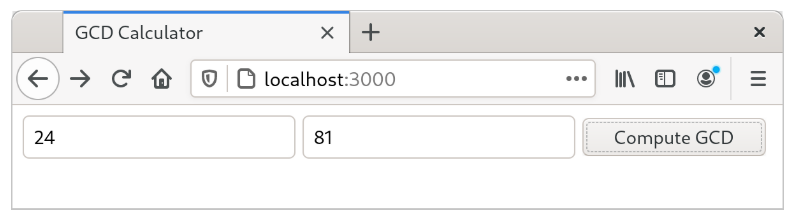
\includegraphics[width=0.8\textwidth]{../img/f2-1.png}
    \caption{提供计算最大公约数功能的web页面}
    \label{f2-1}
\end{figure}

首先,我们需要使用Cargo创建一个新的包,名称为\texttt{actix-gcd}:
\begin{minted}{text}
    $ cargo new actix-gcd
        Created binary (application) `actix-gcd' package
    $ cd actix-gcd
\end{minted}

然后,我们将编辑项目中的\texttt{Cargo.toml}文件来列举出我们需要的包,它的内容如下所示:
\begin{minted}{toml}
    [package]
    name = "actix-gcd"
    version = "0.1.0"
    authors = ["You <you@example.com>"]
    edition = "2018"

    # See more keys and their definitions at
    # https://doc.rust-lang.org/cargo/reference/manifest.html

    [dependencies]
    actix-web = "1.0.8"
    serde = { version = "1.0", features = ["derive"] }
\end{minted}

\texttt{Cargo.toml}中\texttt{dependencies}节的每一行都有一个cartes.io上的crate的名字和需要使用的版本。在这个例子中,我们需要\texttt{actix-web} crate的\texttt{1.0.8}版本和\texttt{serde} crate的\texttt{1.0}版本。crates.io上这两个crate可能还有更新的版本,但是通过指定我们测试成功的特定版本,可以保证即使这两个crate发布了新的版本,代码仍然可以正常工作。我们将会在\hyperref[ch08]{第8章}中详细的讨论版本管理。

crate有一些可选的特性:这些特性是有些用户可能用不到、但仍然需要包含在crate中的部分接口或实现。\texttt{serde}提供了一个非常简洁的方式来处理web表单中的数据,但是根据\texttt{serde}的文档,只有当我们选择了这个crate的\texttt{derive}特性,才可以使用这种方式,因此我们在\texttt{Cargo.toml}文件中制定了这个特性。

注意我们只需要指明那些我们直接使用的crate,\texttt{cargo}会自动下载它们依赖的其他crate。

在我们的第一个版本中,我们将保持web服务器的简洁:它将只提供一个页面,提示用户输入要计算的数字。将\texttt{actix-gcd/src/main.rs}中的内容替换为如下:
\begin{minted}{Rust}
    use actix_web::{web, App, HttpResponse, HttpServer};

    fn main() {
        let server = HttpServer::new( || {
            App::new()
                .route("/", web::get().to(get_index))
        });

        println!("Servering on http://localhost:3000...");
        server
            .bind("127.0.0.1:3000").expect("error binding server to     address")
            .run().expect("error running server");

    }

    fn get_index() -> HttpResponse {
        HttpResponse::Ok()
            .content_type("text/html")
            .body(
                r#"
                    <title>GCD Calculator</title>
                    <form action="/gcd" method="post">
                    <input type="text" name="n"/>
                    <input type="text" name="m"/>
                    <button type="submit">Compute GCD</button>
                    </form>
                "#
            )
    }
\end{minted}

我们以一条\texttt{use}声明开始,引入一些\texttt{actix-web}的定义。当我们写下\texttt{use actix\_web::\{...\}}时,花括号里的每一个名称都被导入到作用域中,这样我们就可以直接使用\texttt{HttpResponse},而不用每次都写出全名\texttt{actix\_web::HttpResponse}。(我们稍后才会使用\texttt{serde} crate)

我们的\texttt{main}函数很简单:它首先调用\texttt{HttpServer::new}来创建一个服务器,这个服务器会响应对\texttt{"/"}路径的get方法;然后打印出一条消息;最后让服务器监听本地机器上的3000 TCP端口。

我们传递给\texttt{HttpServer::new}的参数是Rust的\emph{闭包}表达式\texttt{|| \{ App::new() ... \}}。闭包是一种可以被当作函数来调用的值。这里定义的闭包没有参数,但如果需要参数的话,要写在\texttt{||}之间。\texttt{\{ ... \}}是闭包的函数体。当我们启动服务器时,Actix会启动一个线程池来处理到达的请求。每一个线程都会调用我们的闭包来获取一个\texttt{App}的拷贝,\texttt{App}的值将告诉它如何路由和处理请求。

闭包会调用\texttt{App::new}来创建一个新的、空的\texttt{App}并调用它的\texttt{route}方法来添加一个路径\texttt{"/"}的路由。用\texttt{web::get().to(get\_index)}为这个路由添加处理函数,作用是遇到HTTP \texttt{GET}请求时调用函数\texttt{get\_index}。\texttt{route}方法会返回调用它的\texttt{App}自身,并增加新的路由。因为闭包的结尾处没有分号,因此\texttt{App}就是闭包的返回值,\texttt{HttpServer}线程将会使用它。

\texttt{get\_index}函数构建了一个\texttt{HttpResponse}类型的值作为HTTP \texttt{GET /}请求的响应。\texttt{HttpResponse::Ok()}代表HTTP \texttt{200 OK}状态,表示请求被成功处理。我们还调用了它的\texttt{content\_type}和\texttt{body}方法来填充相应的细节;每一个调用都会返回调用它们的\texttt{HttpResponse}。最后,\texttt{body}方法的返回值作为\texttt{get\_index}的返回值。

因为相应的文本中包含很多双引号,所以我们使用了Rust的raw string语法:字母\texttt{r}、0个或多个井号(\texttt{\#}字符)、一个双引号,string的内容、最后以另一个双引号加上和开头处相同数量的井号结尾。raw string中出现的任何字符都不会被转义,包括双引号;事实上,没有转移的序列例如\texttt{\textbackslash"}也可以被识别。我们可以通过增多井号的数量来保证终止的标记不会出现在字符串内容中。

编写完\texttt{main.rs}之后,我们可以使用\texttt{carto run}命令来运行它:它会自动获取所需的crate、编译它们、编译我们自己的程序、并链接在一起、然后启动它:
\begin{minted}{text}
    $ cargo run
        Updating crates.io index
     Downloading crates ...
      Downloaded serde v1.0.100
      Downloaded actix-web v1.0.8
      Downloaded serde_derive v1.0.100
    ...
      Compiling serde_json v1.0.40
      Compiling actix-router v0.1.5
      Compiling actix-http v0.2.10
      Compiling awc v0.2.7
      Compiling actix-web v1.0.8
      Compiling gcd v0.1.0 (/home/jimb/rust/actix-gcd)
       Finished dev [unoptimized + debuginfo] target(s) in 1m 24s
        Running `/home/jimb/rust/actix-gcd/target/debug/actix-gcd`
    Serving on http://localhost:3000...
\end{minted}

到目前为止,我们可以可以访问给定的URL并看到如\hyperref[f2-1]{图2-1}所示的页面。

不幸的是,点击GCD并不会做任何事,而且会把我们的浏览器导航到一个空页面。接下来让我们来修复它,通过向我们的\texttt{App}添加另一个路由来处理我们表单的\texttt{POST}请求的响应。

终于到了使用我们在\texttt{Cargo.toml}中列出的\texttt{serde} crate的时候了:它提供了一种帮助我们处理表单数据的简单方法。首先,我们需要在\texttt{src/main.rs}中添加如下\texttt{use}声明:
\begin{minted}{Rust}
    use serde::Deserialie;
\end{minted}

Rust程序员通常会把\texttt{use}声明集中在文件开始处,但这并不是必须的:Rust允许\texttt{use}声明以任何顺序出现,只要它们出现在正确的嵌套层级。

接下来让我们定义一个Rust结构体类型来表示我们希望从表单中接收到的数据:
\begin{minted}{Rust}
    #[derive(Deserialize)]
    struct GcdParameters {
        n: u64,
        m: u64,
    }
\end{minted}

这里定义了一个新的类型叫做\texttt{GcdParameters},它有两个字段\texttt{n}和\texttt{m},都是\texttt{u64}类型,和\texttt{gcd}函数的参数类型保持一致。

\texttt{struct}定义上方的注解是一个属性,类似于我们之前用来标记为测试函数时使用的\texttt{\#[test]}属性。在一个类型定义前加上\texttt{\#[derive(Deserialize)]}属性可以告诉\texttt{serde} crate在程序编译时自动为该类型生成代码来把HTML \texttt{POST}请求的表单数据转为该类型的值。事实上,这个属性可以让你从几乎所有结构化的数据:JSON、YAML、TOML或其他文本或二进制格式中解析出一个\texttt{GcdParameters}类型的值。\texttt{serde} crate还提供一个\texttt{Serialize}属性来做相反的事,即把Rust值写成结构化的格式。

有了上面的定义,我们可以简单的写出我们的处理函数:
\begin{minted}{Rust}
    fn post_gcd(form: web::Form<GcdParameters>) -> HttpResponse {
        if form.n == 0 || form.m == 0 {
            return HttpResponse::BadRequest()
                .content_type("text/html")
                .body("Computing the GCD with zero is boring.");
        }

        let response = 
            format!("The greatest common divisor of the numbers {} and {} \
                    is <b>{}</b>\n",
                    form.n, form.m, gcd(form.n, form.m));
        
        HttpResponse::Ok()
            .content_type("text/html")
            .body(response)
    }
\end{minted}

作为Actix请求的处理函数,它的参数的类型必须是Actix知道怎么从中提取出HTTP请求的类型。我们的\texttt{post\_gcd}函数有一个参数\texttt{form},它的类型是\texttt{web::Form<GcdParameters>}。当且仅当\texttt{T}可以从HTML的\texttt{POST}表单数据反序列化出来时,Actix才知道怎么\texttt{web::Form<T>}类型中提取出值。因为我们在\texttt{GcdParameters}类型的定义前加上了\texttt{\#[derive(Deserialize)]}属性,所以Actix可以从表单数据中反序列化出它,因此请求的处理函数可以使用\texttt{web::Form<GcdParameters>}作为参数。这些类型和函数之间的关系都是在编译期处理的,如果你用了Actix不知道该如何处理的类型作为参数的类型,Rust编译器将会立刻告诉你这个错误。

再看\texttt{post\_gcd}的实现:如果有参数的值为0,这个函数会返回一个HTTP \texttt{401 BAD REQUEST}错误,因为这种情况下我们的\texttt{gcd}函数会panic。然后,它使用\texttt{format!}宏创建了一个响应。\texttt{format!}宏类似于\texttt{println!}宏,只不过它不会把字符串写入到标准输出,而是会返回字符串。当响应的文本就绪后,\texttt{post\_gcd}用一个HTTP \texttt{200 OK}响应来包装它,设置好content type之后,就把它返回到请求方。

我们还要把\texttt{post\_gcd}注册为表单的处理函数。我们要把\texttt{main}函数替换为如下内容:
\begin{minted}{Rust}
    fn main() {
        let server = HttpServer::new(|| {
            App::new()
                .route("/", web::get().to(get_index))
                .route("/gcd", web::post().to(post_gcd))
        });

        println!("Servering on http://localhost:3000...");
        server
            .bind("127.0.0.1:3000").expect("error binding server to address")
            .run().expect("error running server");
    }
\end{minted}

唯一的变化在于多了一个\texttt{route}的调用,把\texttt{web::post().to(post\_gcd)}注册为路径\texttt{"/gcd"}的handler。

最后剩余的部分是我们之前编写的\texttt{gcd}函数,要把它添加到\texttt{actix-gcd/src/main.rs}文件中。完成这些之后,你可以停止之前运行的服务器并重新启动程序:
\begin{minted}{text}
    $ cargo run
    Compiling actix-gcd v0.1.0 (/home/jimb/rust/actix-gcd)
     Finished dev [unoptimized + debuginfo] target(s) in 0.0 secs
      Running `target/debug/actix-gcd`
    Serving on http://localhost:3000...
\end{minted}

这一次,通过访问\emph{http://localhost:3000},输入一些数字,然后点击Compute GCD按钮,你应该能看到如下的结果(\hyperref[f2-2]{图2-2})。
\begin{figure}[htbp]
    \centering
    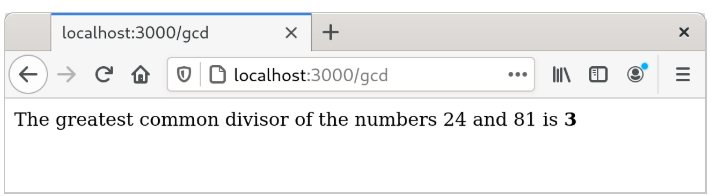
\includegraphics[width=0.8\textwidth]{../img/f2-2.png}
    \caption{显示计算GCD结果的web页面}
    \label{f2-2}
\end{figure}

\section{并发}
Rust的另一项长处是对并发编程的支持。Rust中用于避免内存安全问题的规则同样可以保证线程之间在没有数据竞争的情况下共享数据。例如:
\begin{itemize}
    \item 如果你使用自旋锁来同步需要修改共享数据结构的线程,Rust保证只有当你持有锁的情况下才可以访问数据,并且当你处理完数据后自动释放锁。在C和C++中,自旋锁和要保护的数据之间的关系一般都写在注释里。
    \item 如果你想在几个线程中共享只读数据,Rust保证你不可能意外修改数据。在C和C++中,类型系统也可以帮我们做到这一点,但很容易出错。
    \item 如果你把一个数据结构的所有权从一个线程转移到另一个线程,Rust保证你确实已经失去了对它的访问权。在C和C++中,需要由你自己来保证发送线程不会再次访问该数据。如果你没有正确做到这些,那么结果将会却决于处理器的缓存和你最近写入了多少内存。
\end{itemize}

在这一节中,我们将带领你编写你的第二个多线程程序。

你已经编写过第一个多线程程序了:你用来实现最大公约数服务器的Actix web框架使用了线程池来运行请求的处理函数。如果服务器同时收到很多请求,它会立刻在若干个线程里运行\texttt{get\_form}和\texttt{post\_gcd}函数。这可能让我们有些震惊,因为当我们编写那些函数时我们完全没有并发的概念。

不过Rust保证这么做是安全的,不管你的服务器变得多复杂:只要你的程序能够编译,它就能免于数据竞争。所有的Rust函数都是线程安全的。

这一节的程序将绘制曼德勃罗集,它是一种通过迭代一个简单的复数函数得到的分形。绘制曼德勃罗集经常被称为\emph{embarrassingly parallel}算法,因为线程之间的通信太过简单;我们将会在\hyperref[ch19]{第19章}中讲述更为复杂的模式,但这个例子已经可以展示出一些核心的部分。

开始之前,我们要创建一个新的Rust项目:
\begin{minted}{text}
    $ cargo new mandelbrot
         Created binary (application) `mandelbrot` package
    $ cd mandelbrot
\end{minted}

所有的代码都会添加到\texttt{mandelbrot/src/main.rs}里,我们将会把一些依赖添加到\texttt{mandelbrot/Cargo.toml}。

在开始实现并行的曼德勃罗集之前,我们需要先描述一下我们准备实现的计算过程。

\subsection{曼德勃罗集到底是什么}
了解这一点可以帮我们在阅读代码时更加清楚它要做什么,因此首先让我们先探讨一些纯数学只是。我们将以一个简单的例子开始,并逐渐添加复杂的细节,直到我们讲到曼德勃罗集的核心。

首先这里有一个无限循环,用Rust的语法来写的话就是一个\texttt{loop}语句:
\begin{minted}{Rust}
    fn square_loop(mut x: f64) {
        loop {
            x = x * x;
        }
    }
\end{minted}

在现实中,Rust可能会看出\texttt{x}的值从来没有被使用过,因此并不执行计算。但一开始,首先让我们假设代码按照我们所写的运行。\texttt{x}的值将会发生什么变化?任何小于1的数平方都会变得更小,因此它会接近于0;1的平方还是1;大于1的数平方会变得更大,因此它会接近无限大;负数的平方将会使它变为整数,然后它的变化就和前面说的一样(\hyperref[f2-3]{图2-3})。
\begin{figure}[htbp]
    \centering
    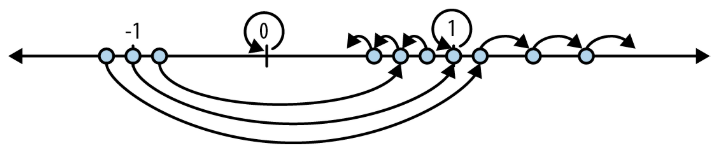
\includegraphics[width=0.8\textwidth]{../img/f2-3.png}
    \caption{重复平方一个数的结果}
    \label{f2-3}
\end{figure}

因此根据传递给\texttt{square\_loop}的值不同,\texttt{x}可能会保持0或者1不变,也可能接近0或者接近无限大。

现在让我们考虑一个稍有不同的循环:
\begin{minted}{Rust}
    fn square_add_loop(c: f64) {
        let mut x = 0.;
        loop {
            x = x * x + c;
        }
    }
\end{minted}

这一次,\texttt{x}从0开始,并且每次迭代时平方之后再加上\texttt{c}。这导致我们更难看出\texttt{x}会怎么变化,但一些实验表明如果\texttt{c}大于\texttt{0.25}或者小于\texttt{-2.0},那么\texttt{x}将会变得接近无穷大;否则它会保持在接近0的某个区间。

更进一步,如果不用\texttt{f64}类型的值,考虑使用复数来执行相同的循环。crates.io上的\texttt{num} crate提供了一个我们可以使用的复数类型,因此我们必须在我们程序的\texttt{Cargo.toml}文件的\texttt{[dependencies]}节中添加一行对\texttt{num}的引用。这是到目前为止这个文件里的全部内容(稍后我们还会添加一些内容):
\begin{minted}{toml}
    [package]
    name = "mandelbrot"
    version = "0.1.0"
    authors = ["You <you@example>"]
    edition = "2018"

    # See more keys and their definitions at
    # https://doc.rust-lang.org/cargo/reference/manifest.html

    [dependencies]
    num = "0.4"
\end{minted}

现在我们可以写出循环的倒数第二个版本:
\begin{minted}{Rust}
    use num::Complex;

    fn complex_square_add_loop(c: Complex<f64>) {
        let mut z = Complex { re: 0.0, im: 0.0};
        loop {
            z = z * z + c;
        }
    }
\end{minted}

用\texttt{z}表示复数是一种习惯,因此我们重命名了变量。表达式\texttt{Complex \{ re: 0.0, im: 0.0 \}}创建了一个\texttt{num} crate的\texttt{Complex}类型的复数0值。\texttt{Complex}时一个Rust的结构体类型,定义类似于如下:
\begin{minted}{Rust}
    struct Complex<T> {
        /// Real portion of the complex number
        re: T,

        /// Imaginary portion of the complex number
        im: T,
    }
\end{minted}

上面的代码定义了一个叫\texttt{Complex}的结构体,有两个字段:\texttt{re}和\texttt{im}。\texttt{Complex}是一个\emph{泛型}结构体:你可以将类型名后的\texttt{<T>}理解为“任意类型\texttt{T}”。例如,\texttt{Complex<f64>}是一个\texttt{re}和\texttt{im}字段都是\texttt{f64}类型的复数,\texttt{Complex<f32>}则是32位浮点数,等等。有了这个定义之后,类似于\texttt{Complex \{ re: 0.24, im: 0.3 \}}这样的表达式将会产生一个\texttt{re}字段初始化为0.24、\texttt{im}字段初始化为0.3的\texttt{Complex}类型的值。

\texttt{num} crate为\texttt{Complex}类型的值提供了\texttt{*, +}和其他的算术运算符,因此剩余的代码就和之前一样,除了它现在是操作复数类型,而不是实数。我们将会在\hyperref[ch12]{第12章}解释怎么为自定义类型定义运算符。

最后,我们终于完成了纯数学的部分。曼德勃罗集被定义为使得\texttt{z}不会变为无穷大的\texttt{c}的集合。我们最初始版本的循环很容易预测结果:任何大于1或小于-1的数都不满足。每次迭代平方之后再\texttt{+ c}让程序的行为更难预测:正如我们之前所说的那样,如果\texttt{c}的值大于0.25或者小于-2会导致\texttt{z}变为无穷大。但如果扩展到复数领域事情就会变得有趣起来,并且会生成漂亮的图形,我们将绘制这个图形。

因为一个复数\texttt{c}同时有实部\texttt{c.re}和虚部\texttt{c.im},因此我们将它当作笛卡尔坐标系中的\texttt{x}和\texttt{y}坐标,然后如果\texttt{c}在曼德勃罗集里就把点设置为黑色,否则设置为白色。因此对于我们图片中的每个像素点,我们必须运行复数版本的循环,看看它最终是会变为无穷大还是围绕在原点附近,并以次判断点的颜色。

无限循环会运行很长时间,但有两个技巧可以加快它。首先,如果我们放弃无限循环而是只迭代有限次,实验表明我们仍然可以得到一个不错的近似结果。迭代多少次取决于我们想要多精确的绘制边界。其次,已经被证明的一点是,如果\texttt{z}有一次离开了以原点为中心半径为2的圆形范围,它将会逐渐变为无穷大。因此这是我们最终版本的循环,也是我们程序的核心:
\begin{minted}{Rust}
    use num::Complex;

    /// Try to determine if `c` is in the Mandelbrot set, using at most `limit`
    /// iterations to decide.
    ///
    /// If `c` is not a member, return `Some(i)`, where `i` is the number of
    /// iterations it took for `c` to leave the circle of radius 2 centered on the
    /// origin. If `c` seems to be a number (more precisely, if we reached the
    /// iteration limit without being able to prove that `c` is not a member),
    /// return `None`.
    fn escape_time(c: Complex<f64>, limit: usize) -> Option<usize> {
        let mut z = Complex { re: 0.0, im: 0.0 };
        for i in 0..limit {
            if z.norm_sqr() > 4.0 {
                return Some(i);
            }
            z = z * z + c;
        }
        None
    }
\end{minted}

这个函数接收我们想测试是否在曼德勃罗集中的复数\texttt{c}和迭代次数上限作为参数。函数的返回值是\texttt{Option<usize>}类型。Rust的标准库中\texttt{Option}类型定义如下:
\begin{minted}{Rust}
    enum Option<T> {
        None,
        Some(T),
    }
\end{minted}

\texttt{Option}是一个\emph{枚举类型},通常被称为\emph{enum},因为它的定义列举出了一个该类型的实例可能的值:对于任何类型\texttt{T},一个\texttt{Option<T>}类型的值要么是\texttt{Some(v)}(其中\texttt{v}是\texttt{T}类型的值),要么是\texttt{None},表示没有可用的\texttt{T}类型的值。类似于我们之前讨论的\texttt{Complex}类型,\texttt{Option}也是泛型类型:你可以用\texttt{Option<T>}来代替任何类型的可选值。

在我们的例子中,\texttt{escape\_time}返回一个可选的\texttt{Option<usize>}来表示\texttt{c}是否在曼德勃罗集里——如果不在的话,我们需要多少次迭代才能知道它不在。如果\texttt{C}不在曼德勃罗集里,\texttt{escape\_time}会返回\texttt{Some(i)},其中\texttt{i}是\texttt{z}离开半径为2的圆所需的迭代次数。否则,如果\texttt{c}在曼德勃罗集里,\texttt{escape\_time}会返回\texttt{None}。
\begin{minted}{Rust}
    for i in 0..limit {
\end{minted}

更早的例子中展示过使用\texttt{for}循环迭代命令行参数和vector的元素;这里的\texttt{for}循环迭代一个从\texttt{0}到\texttt{limit}(但不包含)的范围内的整数。

\texttt{z.norm\_sqr()}方法会返回\texttt{z}与原点的距离的平方。为了判断\texttt{z}是否离开了半径为2的圆,我们不需要求平方根,只需要比较距离的平方和4.0即可,这样会更快一些。

你可能已经注意到我们在函数定义的上方使用了\texttt{///}来标记注释行;\texttt{Complex}结构体的成员上方的注释也是以\texttt{///}开头。这些事\emph{文档注释};\texttt{rustdoc}工具知道该如何解析它们、收集它们中对代码的解释、并生成在线文档。Rust标准库的文档就是用这种方式书写的。我们将在\hyperref[ch08]{第8章}中详细介绍文档注释。

程序的剩余部分就是在多大的分辨率范围内计算曼德勃罗集和把负载分发到若干线程来加快计算。

\subsection{解析成对的命令行参数}
程序将会接收几个命令行参数来控制生成图片的分辨率和图中曼德勃罗集所占的部分。因为这些命令行参数都遵循相同的形式,这里定义了一个解析它们的函数:
\begin{minted}{Rust}
    use std::str::FromStr;

    /// Parse the string `s` as a coordinate pair, like `"400x6000"` or `"1.0,0.5"`
    ///
    /// Specifically, `s` should have the form <left><sep><right>, where <sep> is
    /// the character given by the `separator` argument, and <left> and <right> are
    /// both strings that can be parsed by `T::from_str`, `separator` must be an
    /// ASCII character.
    ///
    /// If `s` has the proper form, return `Some<(x, y)>`. If it doesn't parse
    /// correctly, return `None`.
    fn parse_pair<T: FromStr>(s: &str, separator: char) -> Option<(T, T)> {
        match s.find(separator) {
            None => None,
            Some(index) => {
                match (T::from_str(&s[..index]), T::from_str(&s [index + 1..])) {
                    (Ok(l), Ok(r)) => Some((l, r)),
                    _ => None
                }
            }
        }
    }

    #[test]
    fn test_parse_pair() {
        assert_eq!(parse_pair::<i32>("",        ','), None);
        assert_eq!(parse_pair::<i32>("10,",     ','), None);
        assert_eq!(parse_pair::<i32>(",10",     ','), None);
        assert_eq!(parse_pair::<i32>("10,20",   ','), Some((10, 20)));
        assert_eq!(parse_pair::<i32>("10,20xy", ','), None);
        assert_eq!(parse_pair::<f64>("0.5x",    ','), None);
        assert_eq!(parse_pair::<f64>("0.5x1.5", 'x'), Some((0.5, 1. 5)));
    }
\end{minted}

\texttt{parse\_pair}的定义是一个\emph{泛型函数}:
\begin{minted}{Rust}
    fn parse_pair<T: FromStr>(s: &str, separator: char) -> Option<(T, T)> {
\end{minted}

你可以将语法\texttt{<T: FromStr>}读作:“对于任意实现了\texttt{FromStr} trait的类型\texttt{T}...”。这可以让我们方便的一次定义一系列函数:\texttt{parse\_pair::<i32>}是一个把字符串解析为\texttt{i32}值对的函数,\texttt{parse\_pair::<f64>}是一个吧字符串解析为浮点数对的函数,等等。这很像C++中的函数模板。一个Rust程序员会把\texttt{T}称为\emph{parse\_pair}的\emph{类型参数}。当你使用泛型函数时,Rust通常能推导出类型参数,你不需要像我们测试代码中那样指明类型。

我们的返回类型是\texttt{Option<(T, T)>}:要么是\texttt{None}要么是\texttt{Some((v1, v2))},\texttt{(v1, v2)}是一个有两个值的元组,两个值类型都是\texttt{T}。\texttt{parse\_pair}函数没有使用显式的return语句,因此它的返回值就是函数体中最后一条表达式的值:
\begin{minted}{Rust}
    match s.find(separator) {
        None => None,
        Some(index) => {
            ...
        }
    }
\end{minted}

\texttt{String}类型的\texttt{find}方法会在字符串中搜索匹配\texttt{separator}的字符。如果\texttt{find}返回\texttt{None},表示字符串中不存在分隔字符,整个\texttt{match}语句将会求值为\texttt{None},表示解析失败;否则,\texttt{index}就是分隔字符在字符串中的位置。

\begin{minted}{Rust}
    match (T::from_str(&s[..index]), T::from_str(&s[index + 1..])) {
        (Ok(l), Ok(r)) => Some((l, r)),
        _ => None
    }
\end{minted}

从这里就能看出\texttt{match}表达式的强大,要匹配的参数是这个元组表达式:
\begin{minted}{Rust}
    (T::from_str(&s[..index]), T::from_str(&s[index + 1..]))
\end{minted}
表达式\texttt{\&s[..index]}和\texttt{\&s[index + 1..]}是字符串切片,分别是分隔字符之前和之后的部分。参数\texttt{T}的类型关联的\texttt{from\_str}函数接收参数并尝试将它们解析为\texttt{T}类型的值,最后生成一个元组。我们要匹配的模式是:
\begin{minted}{Rust}
    (Ok(l), Ok(r)) => Some((l, r)),
\end{minted}

只有当元组的两个值都是\texttt{Result}类型的\texttt{Ok}值才可以匹配这个模式,表示两个解析都成功了此时\texttt{Some((l, r))}。就是match表达式的值,也是函数的返回值。

\begin{minted}{Rust}
    _ => None
\end{minted}

通配模式\texttt{\_}匹配任何情况并忽略值。如果我们到达这个地方,说明\texttt{parse\_pair}失败了,因此求值为\texttt{None},并作为函数的返回值。

现在我们已经有了\texttt{parse\_pair},很容易就可以写出一个解析一对浮点数并返回\texttt{Complex<f64>}值的函数:
\begin{minted}{Rust}
    /// Parse a pair of floating-point numbers separated by a comma as a complex
    /// number.
    fn parse_complex(s: &str) -> Option<Complex<f64>> {
        match parse_pair(s, ',') {
            Some((re, im)) => Some(Complex { re, im }),
            None => None
        }
    }

    #[test]
    fn test_parse_complex() {
        assert_eq!(parse_complex("1.25,-0.0625"),
                   Some(Complex { re: 1.25, im: -0.0625 }));
        assert_eq!(parse_complex(",-0.0625"), None);
    }
\end{minted}

\texttt{parse\_complex}函数会调用\texttt{parse\_pair}函数,如果参数成功解析就构建一个\texttt{Complex}值,如果失败就向调用者传播。

如果你仔细阅读代码,你可能已经注意到我们使用了一种简写的方式来构建\texttt{Complex}值。用同名的变量来初始化结构体的字段是很常见的,因此相比于强迫你写\texttt{Complex \{ re: re, im: im \}},Rust允许你简写为\texttt{Complex \{ re, im \}}。这是受JavaScript和Haskell中类似写法的启发。

\subsection{将像素映射到复数}
我们的程序需要处理两个相关联的坐标空间:输出图片中的每个像素对应复平面中的一个点。这两个空间的关系取决于我们要绘制的曼德勃罗集的部分和图片的分辨率,这些都是命令行参数决定的。下面的函数实现从\emph{图片空间}到\emph{复数空间}的转换:
\begin{minted}{Rust}
    /// Given the row and column of a pixel in the output image, return the
    /// corresponding point on the complex plane.
    ///
    /// `bounds` is a pair giving the width and height of the image in pixels.
    /// `pixel` is a (column, row) pair indicating a particular pixel in that image.
    /// The `upper_left` and `lower_right` parameters are points on the complex
    /// plane designating the area our image covers.
    fn pixel_to_point(bounds: (usize, usize),
                      pixel: (usize, usize),
                      upper_left: Complex<f64>,
                      lower_right: Complex<f64>) -> Complex<f64> {
        let (width, height) = (lower_right.re - upper_left.re,
                               upper_left.im - lower_right.im);
        Complex {
            re: upper_left.re + pixel.0 as f64 * width / bounds.0 as f64,
            im: upper_left.im - pixel.1 as f64 * height / bounds.1 as f64
            // Why subtraction here? pixel.1 increases as we go down,
            // but the imaginary component increases as we go up.
        }
    }

    #[test]
    fn test_pixel_to_point() {
        assert_eq!(pixel_to_point((100, 200), (25, 175),
                                  Complex { re: -1.0, im: 1.0 },
                                  Complex { re: 1.0, im: -1.0 }),
                   Complex { re: -0.5, im: -0.75 });
    }
\end{minted}

\hyperref[f2-4]{图2-4}展示了\texttt{pixel\_to\_point}进行的计算。

\begin{figure}[htbp]
    \centering
    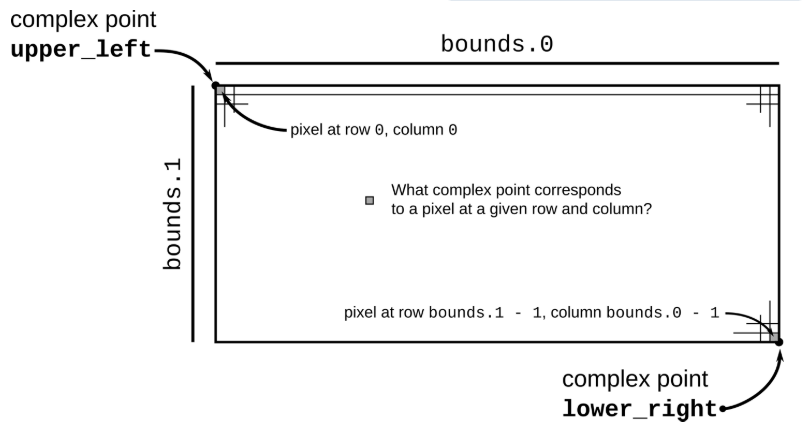
\includegraphics[width=0.8\textwidth]{../img/f2-4.png}
    \caption{复数平面和图片像素的关系}
    \label{f2-4}
\end{figure}

\texttt{pixel\_to\_point}中的代码只是简单的计算,因此我们不会详细解释。然而,还是有一点要提一下。下面的表达式展示了引用元组元素的方式:
\begin{minted}{Rust}
    pixel.0
\end{minted}
上面的表达式引用了元组\texttt{pixel}的第一个元素。

\begin{minted}{Rust}
    pixel.0 as f64
\end{minted}

这是Rust的类型转换语法:把\texttt{pixel.0}转换为\texttt{f64}类型的值。与C和C++不同,Rust禁止数字类型之间的隐式转换,你必须显式写明类型转换。这可能会很枯燥,但显式指明类型转换有时会很有用。整数之间的隐式转换看起来似乎没有问题,但历史上在真实世界的C和C++代码中它们导致了很多的bug和安全漏洞。

\subsection{绘制曼德勃罗集}

    \chapter{基本类型}\label{ch03}
\emph{这个世界上有很多很多不同类型的书,这是一件好事。但也有很多很多不同类型的人,每个人都想读到一些不同的东西。}
\begin{flushright}
    ——Lemony Snicket
\end{flushright}

在很大程度上,Rust语言是围绕它的类型来设计的。它对高性能代码的支持源于让开发者选择不同情况下最合适的数据表示,并在简单性和成本之间取得适当的平衡。Rust的内存和线程安全也依赖于类型系统的健全性,Rust的灵活性则来自于它的泛型和trait。

这一章将介绍Rust的基本类型。这些源码级别的类型都有对应的成本和性能可预测的机器级的组件。尽管Rust并不保证它会完全按照你的要求精确的表示数据,但只有当它是一个可靠的改进时它才会违背你的要求。

与JavaScript或Python这种动态类型语言相比,Rust要求你事先就进行更多规划。你必须写出函数参数和返回值、结构体字段、以及一些其他结构的类型。然而,Rust的两个特性使得这比你想象中的要简单很多:

\begin{itemize}
    \item 有了你指明的类型,Rust的\emph{类型推导}将会为你推导出剩余的大部分类型。在实践中,通常只有一个类型能够满足给定的变量或表达式。在这种情况下,Rust允许你留空,或者说\emph{省略}这个类型。例如,你可以像下面这样写出一个函数里的所有类型:
          \begin{minted}{Rust}
    fn build_vector() -> Vec<i16> {
        let mut v: Vec<i16> = Vec::<i16>::new();
        v.push(10i16);
        v.push(20i16);
        v
    }
    \end{minted}
          但这非常杂乱和重复。给定了函数的返回值之后,很明显\texttt{v}必须是\texttt{Vec<i16>}类型:一个16位有符号整数的vector,没有其他的类型可以满足语义。并且据此可以推出vector的每个元素必须是\texttt{i16}类型。这就是Rust的类型推导适用的场景,所以你可以改为:
          \begin{minted}{Rust}
    fn build_vector() -> Vec<i16> {
        let mut v = Vec::new();
        v.push(10);
        v.push(20);
        v
    }
    \end{minted}
          这两个定义是完全等价的,Rust将会生成完全相同的机器代码。类型推导可以回馈一部分动态类型语言的可读性,并且仍能在编译时捕捉到类型错误。
    \item 函数可以是\emph{泛型}的:一个函数可以同时处理很多不同类型的值。

          在Python和JavaScript中,所有的函数都很自然的是泛型的:一个函数可以操作任何类型的值,只要这个类型有函数体中需要的属性和方法。(这种特性通常被称作\emph{鸭子类型}:如果它像鸭子一样叫,那它就是一只鸭子。)但正是这种灵活性也导致这些语言很难检测出类型错误,在这些语言里测试通常是唯一一种捕捉类型错误的方式。Rust的泛型函数给予了这门语言某种程度上和动态类型同样的灵活性,并且仍能在编译期捕获所有的类型错误。

          除了灵活性之外,泛型函数和非泛型的函数一样高效。例如,为每个整数类型都编写一个\texttt{sum}函数与编写一个处理所有整数类型的泛型\texttt{sum}函数相比,并没有性能上的优势。我们将在\hyperref[ch11]{第11章}种详细讨论泛型函数。
\end{itemize}

这一章的剩余部分将会自上而下的覆盖Rust的类型,从最简单的数字类型例如证书和浮点数到持有多个值的复合类型:box、tuple、数组和字符串。

这里有一个Rust中类型的汇总。\hyperref[t3-1]{表3-1}显示了Rust的原始类型,包括一些来自标准库的基本类型,和一些用户自定义类型的示例。

\begin{longtable}{p{0.25\textwidth}p{0.4\textwidth}p{0.25\textwidth}}
    \caption{Rust中的类型示例}
    \label{t3-1}\\
    \hline
    \textbf{类型}   & \textbf{描述}    & \textbf{值}    \\
    \hline
    \texttt{i8, i16, i32, i64, i128, u8, u16, u32, u64, u128}    & 指定位数的有符号和无符号整数 & \texttt{42, -5i8, 0x400u16, 0o100i16, 20\_922\_789\_888\_000u64, b'*'(u8字节字面量)}    \\
    \rowcolor{tablecolor}
    \texttt{isize, usize}   & 有符号和无符号整数,和机器里的一个指针一样大(32位或64位)   & \texttt{137, -0b0101\_0010isize, 0xffff\_fc00usize} \\
    \texttt{f32, f64}       & IEEE浮点数,单精度和双精度                                & \texttt{1.61803, 3.14f32, 6.0221e23f64} \\
    \rowcolor{tablecolor}
    \texttt{bool}           & 布尔值            & \texttt{true, false} \\
    \texttt{char}           & Unicode字符,32位 & \texttt{'*', '\textbackslash n', '字', '\textbackslash x7f', '\textbackslash u\{CA0\}'} \\
    \rowcolor{tablecolor}
    \texttt{(char, u8, i32)}                        & Tuple:把类型混合在一起   & \texttt{('\%', 0x7f, -1)} \\
    \texttt{()}                                     & “单元值”(空tuple)      & \texttt{()} \\
    \rowcolor{tablecolor}
    \texttt{struct S \{ x: f32, y: f32 \}}          & 命名字段结构体            & \texttt{S \{ x: 120.0, y: 209.0 \}} \\
    \texttt{struct T (i32, char);}                  & 元组结构体                & \texttt{T(120, 'X')} \\
    \rowcolor{tablecolor}
    \texttt{struct E;}                              & 元组结构体,无字段        & \texttt{E} \\
    \texttt{enum Attend \{ OnTime, Late(u32) \}}    & 枚举,代数数据类型        & \texttt{Attend::Late(5), Attend::OnTime} \\
    \rowcolor{tablecolor}
    \texttt{Box<Attend}                             & Box:持有一个堆上的值的指针   & \texttt{Box::new(Late(15))} \\
    \texttt{\&i32, \&mut i32}                       & 共享和可变引用:生命周期不能超过所引用对象的无所有权的指针 & \texttt{\&s.y, \&mut v} \\
    \rowcolor{tablecolor}
    \texttt{String}                                 & UTF-8字符串,动态大小         & \texttt{"ラーメン: ramen"\newline.to\_string()} \\
    \texttt{\&str}                                  & \texttt{str}的引用:指向UTF-8字符串的无所有权的指针 & \texttt{"そば: soba", \&s[0..12]} \\
    \rowcolor{tablecolor}
    \texttt{[f64; 4], [u8; 256]}                    & 固定长度的数组,所有元素的类型都必须相同   & \texttt{[1.0, 0.0, 0.0, 1.0], [b' '; 256]} \\
    \texttt{Vec<f64>}                               & 可变长度的vector,所有元素的类型都必须相同 & \texttt{vec![0.367, 2.718, 7.389]} \\
    \rowcolor{tablecolor}
    \texttt{\&[u8], \&mut [u8]}                     & 切片的引用:指向数组或vector的一部分,包含指针和长度 & \texttt{\&v[10..20], \&mut a[..]} \\
    \texttt{Option<\&str>}      & 可选值:\texttt{None}(无值)或\texttt{Some(v)}(有值,值为\texttt{v})   & \texttt{Some("Dr.", None)} \\
    \rowcolor{tablecolor}
    \texttt{Result<u64, Error>} & 可能会失败的操作的结果:成功时是\texttt{Ok(v)},失败时是\texttt{Err(e)} & \texttt{Ok(4096), Err(Error::last\_os\_error())} \\
    \texttt{\&dyn Any, \&mut dyn Read}  & trait对象:指向一个实现了给定方法的任何值 & \texttt{value as \&dyn Any, \&mut file as \&mut dyn Read} \\
    \rowcolor{tablecolor}
    \texttt{fn(\&str) -> bool}          & 函数指针      & \texttt{str::is\_empty}           \\
    (闭包类型)                         & 闭包         & \texttt{|a, b| \{ a*a + b*b \}}    \\
\end{longtable}

这些类型中的大部分都会在这一章中介绍,除了下面这些:
\begin{itemize}
    \item 我们将在\hyperref[ch09]{第9章}中单独介绍\texttt{struct}类型。
    \item 我们将在\hyperref[ch10]{第10章}中单独介绍枚举类型。
    \item 我们将在\hyperref[ch11]{第11章}中介绍trait对象。
    \item 我们将在这里介绍\texttt{String}和\texttt{\&str}的基础,但在\hyperref[ch17]{第17章}中介绍更多细节。
    \item 我们将在\hyperref[ch14]{第14章}介绍函数和闭包类型。
\end{itemize}

\section{固定位数的数字类型}
Rust类型系统的基础是一组固定宽度的数字类型的集合,这些类型和现代处理器中的硬件类型相匹配。

固定宽度的数字类型可能会溢出或失去精度,但它们适用于大多数的类型,并且比任意精度的整数和精确小数快几千倍。如果你需要那些类型的数字,可以在\texttt{num} crate找到相应的支持。

Rust的数字类型的名称遵循通用的模式,宽度加上表示的含义(\hyperref[f3-2]{表3-2})。
\begin{table}[htbp]
    \centering
    \caption{Rust的数字类型}
    \label{f3-2}
    \begin{tabular}{llll}
        \hline
        \textbf{大小(比特数)}   & \textbf{无符号整数}   & \textbf{有符号整数}   & \textbf{浮点数}   \\
        \hline
        \texttt{8}  & \texttt{u8}   & \texttt{i8}   &              \\
        \rowcolor{tablecolor} 
        \texttt{16} & \texttt{u16}  & \texttt{i16}  &              \\
        \texttt{32} & \texttt{u32}  & \texttt{i32}  & \texttt{f32} \\
        \rowcolor{tablecolor} 
        \texttt{64} & \texttt{u64}  & \texttt{i64}  & \texttt{f64} \\
        \texttt{128}& \texttt{u128} & \texttt{i128} &              \\
        \rowcolor{tablecolor} 
        机器字      & \texttt{usize} & \texttt{isize} & \\
    \end{tabular}
\end{table}

这里,\emph{机器字}是运行代码的机器上的一个指针的大小,32位或者64位。

\subsection{整数类型}

Rust的无符号整数使用全部的范围来表示正数和0(\hyperref[t3-3]{表3-3})。
\begin{table}[htbp]
    \centering
    \caption{Rust无符号整数类型}
    \label{t3-3}
    \begin{tabular}{ll}
        \hline
        \textbf{类型}   &   \textbf{范围}                   \\
        \hline
        \texttt{u8}     & 0到$2^{8}-1$(0到255)            \\
        \rowcolor{tablecolor} 
        \texttt{u16}    & 0到$2^{16}-1$(0到65,535)        \\
        \texttt{u32}    & 0到$2^{32}-1$(0到4,294,967,295) \\
        \rowcolor{tablecolor} 
        \texttt{u64}    & 0到$2^{64}-1$(0到18,446,744,073,709,551,615或1万8千亿)  \\
        \texttt{u128}   & 0到$2^{128}-1$(0到大约$3.4*10^{38}$)                    \\
        \rowcolor{tablecolor} 
        \texttt{usize}  & 0到$2^{32}-1$或$2^{64}-1$         \\
    \end{tabular}
\end{table}

Rust的有符号整数使用两种互补的表示方法,使用和无符号类型相对应的位模式来表示一个包含正数和负数的范围(\hyperref[t3-4]{表3-4})。
\begin{table}[htbp]
    \centering
    \caption{Rust的有符号整数类型}
    \label{t3-4}
    \begin{tabular}{ll}
        \hline
        \textbf{类型}   &   \textbf{范围}   \\
        \hline
        \texttt{i8}     & $-2^{7}$到$2^{7}-1$(-128到127)   \\
        \rowcolor{tablecolor}
        \texttt{i16}    & $-2^{15}$到$2^{15}-1$(-32,768到32,767)  \\
        \texttt{i32}    & $-2^{31}$到$2^{31}-1$(-2,147,483,648到2,147,483,647)    \\
        \rowcolor{tablecolor}
        \texttt{i64}    & $-2^{63}$到$2^{63}-1$(-9,223,372,036,854,775,808到9,223,372,036,854,775,807)    \\
        \texttt{i128}   & $-2^{127}$到$2^{127-1}$(大约$-1.7\times10^{38}$到$+1.7\times10^{38}$) \\
        \rowcolor{tablecolor}
        \texttt{isize}  & $-2^{31}$到$2^{31}-1$,或者$-2^{63}$到$2^{63}-1$  \\
    \end{tabular}
\end{table}

Rust使用\texttt{u8}类型来表示一个字节的值。例如,从二进制文件或者套接字读取数据就会返回\texttt{u8}类型的数据流。

与C和C++不同,Rust区分了字符和数字类型:\texttt{char}不是\texttt{u8},也不是\texttt{u32}(尽管它是32位)。我们将会在“\hyperref[char]{字符}”这一节介绍Rust的\texttt{char}类型。

\texttt{usize}和\texttt{isize}类似于C和C++中的\texttt{size\_t}和\texttt{ptrdiff\_t}类型。它们的位数和目标机器上地址空间的位数相同:在32位架构上就是32位,在64位架构上就是64位。Rust要求数组索引为\texttt{usize}类型的值。数组或vector或其他任何含有多个元素的数据结构的长度都是\texttt{usize}类型。

Rust中的整数字面量可以有一个后缀来指示类型:\texttt{42u8}是一个\texttt{u8}类型的值,\texttt{1729isize}是一个\texttt{isize}类型的值。如果一个整数字面量没有类型后缀,Rust将会延迟决定它的类型,直到可以从它的使用中推断出它的类型:存储到一个已知类型的变量中、作为参数传递给一个参数类型已知的函数、和一个已知类型的值比较、以及类似的情况。如果到最后还是有很多类型可以满足,此时如果\texttt{i32}是其中一种可能,Rust将推断它为\texttt{i32}类型。否则,Rust会报歧义错误。

前缀\texttt{0x, 0o, 0b}分别表示十六进制、八进制、二进制字面量。

为了让长数字更更读,你可以在数字中间插入下划线。例如,你可以把最大的\texttt{u32}值写作\texttt{4\_294\_967\_295}。下划线放置的位置并不重要,所以你可以每四位插入一个下划线来把十六进制和二进制数字分组,例如\texttt{0xffff\_ffff}或者在最后插入下划线分隔类型后缀,例如\texttt{127\_u8}。\hyperref[t3-5]{表3-5}给出了一些整数字面量的例子。
\begin{table}[htbp]
    \centering
    \caption{整数字面量的例子}
    \label{t3-5}
    \begin{tabular}{lll}
        \hline
        \textbf{字面量} & \textbf{类型} & \textbf{十进制值} \\
        \hline
        \texttt{116i8}          & \texttt{i8}       &   116 \\
        \rowcolor{tablecolor}
        \texttt{0xcafeu32}      & \texttt{u32}      &   51966 \\
        \texttt{0b0010\_1010}   & 推断              &   42 \\
        \rowcolor{tablecolor}
        \texttt{0o106}          & 推断              &   70 \\
    \end{tabular}
\end{table}

尽管数值类型和\texttt{char}类型是不同的,Rust确实提供了\emph{字节字面量}:很像字符字面量的\texttt{u8}值:\texttt{b'X'}代表字符\texttt{X}的ASCII码值,但是是\texttt{u8}类型的值。例如,因为\texttt{A}的ASCII码值是65,字面量\texttt{b'A'}和\texttt{65u8}是等价的。只有ASCII字符可以出现在字节字面量中。

这里有一些不能用单个字符表示的字符,因为它们要么会导致歧异要么很难看出来。\hyperref[t3-6]{表3-6}中的字符只能用反斜杠转移的方式写出来。
\begin{table}[htbp]
    \centering
    \caption{需要转义的字符}
    \label{t3-6}
    \begin{tabular}{lll}
        \hline
        \textbf{字符}   &   \textbf{字节字面量} & \textbf{等价的数字值} \\
        \hline
        单引号,'   &   \texttt{b'\textbackslash''}      & 39u8 \\
        \rowcolor{tablecolor}
        反斜杠,\textbackslash &    \texttt{b'\textbackslash\textbackslash'} & 92u8 \\
        换行        &    \texttt{b'\textbackslash n'}    & 10u8 \\
        \rowcolor{tablecolor}
        回车        &   \texttt{b'\textbackslash r'}     & 13u8 \\
        制表符      &   \texttt{b'\textbackslash t'}     & 9u8 \\
    \end{tabular}
\end{table}

对于那些难以写出或看出的字符,你可以用它们的十六进制码代替。一个字节字面量的形式是\texttt{b'\textbackslash xHH'},其中\texttt{HH}是两个十六进制的数字,代表值是\texttt{HH}的字节。例如,你可以将ASCII的“escape”字符的字节字面量写作\texttt{b'\textbackslash x1b'},因为“escape”的ASCII码是27,也就是16进制的1B。因为字节字面量只是\texttt{u8}类型值的另一种表示方式,考虑使用数字字面量可能可读性会更强:只有当你想表示ASCII码时\texttt{b'\textbackslash x1b'}才会比\texttt{27}更有意义。

你可以将一种整数类型转换为另一种整数类型。我们将会在“\hyperref[cast]{类型转换}”这一节中介绍转换的原理,这里有一些例子:
\begin{minted}{Rust}
    assert_eq!(   10_i8  as u16,    10_u16); // in range
    assert_eq!( 2525_u16 as i16,  2525_i16); // in range

    assert_eq!(   -1_i16 as i32,    -1_i32); // 符号扩展
    assert_eq!(65535_u16 as i32, 65535_i32); // 0扩展

    // 转换一个超出目标类型范围的值
    // 等价于原值对2^N取模
    // N是目标类型的位数
    // 这有时也被称为“截断”
    assert_eq!( 1000_i16 as  u8,    232_u8);
    assert_eq!(65535_u32 as i16,     -1_i16);

    assert_eq!(   -1_i8  as u8,     255_u8);
    assert_eq!(  255_u8  as i8,      -1_i8);
\end{minted}

标准库提供一些整数的方法来进行操作。例如:
\begin{minted}{Rust}
    assert_eq!(2_u16.pow(4), 16);               // 求指数幂
    assert_eq!((-4_i32).abs(), 4);              // 求绝对值
    assert_eq!(0b101101_u8.count_ones(), 4);    // 位计数
\end{minted}

你可以在在线文档中找到这些。但是注意,文档中\texttt{i32}(原始类型)和模块导入的类型(搜索\texttt{std::i32})有不同的单独页面。

在实际编码时,你不需要像我们在这里一样写出类型后缀,因为上下文会自动推断出类型。当推断不出来时,错误信息可能会让你很惊讶。例如,下面的代码不能编译:
\begin{minted}{Rust}
    println!("{}", (-4).abs());
\end{minted}

Rust报错:
\begin{minted}{text}
    error: can't call method `abs` on ambiguous numeric type `{integer}`
\end{minted}

这可能有点迷惑:所有的整数类型都有\texttt{abs}方法,所以问题在哪呢?从技术角度来说,Rust需要在调用某个类型的方法之前知道这个值的精确类型。只有当所有的方法调用都被解析之后仍然存在歧义才会使用默认的\texttt{i32}类型,而在这里,在解析\texttt{abs}方法时就需要知道\texttt{-4}的类型,默认推导为\texttt{i32}的规则在此时不能生效。解决方法是指明类型,要么加上类型后缀,要么使用类型特定的函数:
\begin{minted}{Rust}
    println!("{}", (-4_i32).abs());
    println!("{}", i32::abs(-4));
\end{minted}

注意函数调用的优先级高于一元前缀运算符,所以当对负数调用方法时一定要小心。如果这个地方第一个表达式里\texttt{-4\_i32}两侧没有括号,\texttt{-4\_i32.abs()}将会对\texttt{4}调用\texttt{abs}方法,返回正数\texttt{4},然后求负数返回\texttt{-4}。

\subsection{Checked、Wrapping、Saturating、Overflowing算术}

当整数运算溢出时,如果是在debug模式下Rust会panic。在release模式下,运算结果会\emph{回环}:它会返回正确的值对结果类型能表示的范围取余之后的结果。(这两种情况下,溢出都不像在C和C++中一样是未定义行为)。

例如,下面的代码在debug模式下会panic:
\begin{minted}{Rust}
    let mut i = 1;
    loop {
        i *= 10;    // panic: 尝试乘到溢出
                    // (但只有在debug模式会panic!)
    }
\end{minted}

在release模式下,溢出时乘法会回环成负数,然后循环会无限执行。

如果默认行为不是你希望的结果,整数类型提供了一个方法让你指定想要做什么。例如,下面的代码在任何构建模式下都会panic:
\begin{minted}{Rust}
    let mut i: i32 = 1;
    loop {
        // panic: 乘法溢出(在任何构建模式下)
        i = i.checked_mul(10).expect("multiplication overflowed");
    }
\end{minted}

这些整数运算的方法可以被分为四个通用的类别:
\begin{itemize}
    \item \emph{Checked}操作返回一个结果的\texttt{Option}值:如果运算结果可以被结果类型正确表示就返回\texttt{Some(v)},否则返回\texttt{None}。例如:
    \begin{minted}{Rust}
    // 10和20的结果可以用u8表示。
    assert_eq!(10_u8).checked_add(20), Some(30));

    // 不幸的是,100和200的和不能用u8表示。
    assert_eq!(100_u8).checked_add(200), None);

    // 求和,如果溢出就panic。
    let sum = x.checked_add(y).unwrap();

    // 奇怪的是,在一种特定情况下,有符号除法也可能会导致溢出。
    // 一个有符号整数能表示-2^(n-1),但不能表示2^(n-1)。
    assert_eq!((-128_i8).checked_div(-1), None);
    \end{minted}

    \item \emph{Wrapping}操作返回正确的值对结果类型能表示的范围的余数:
    \begin{minted}{Rust}
    // 第一个积可以用u16来表示。
    // 第二个不能,因此我们得到250000对2^16取模。
    assert_eq!(100_u16.wrapping_mul(200), 20000);
    assert_eq!(500_u16.wrapping_mul(500), 53392);

    // 有符号数的操作可能会回环成负数。
    assert_eq!(500_i16.wrapping_mul(500), -12144);

    // 在移位操作中,移动的位数会回环到该类型的位数之内
    // 因此对16位的数字移动17位等于移动1位
    assert_eq!(5_i16.wrapping_shl(17), 10);
    \end{minted}
    正如解释的那样,这就是release模式下算术操作的行为。使用这种写法的好处是在所有的构建模式下代码的行为都一致。

    \item \emph{Saturating}操作会返回最接近正确结果的表示。换句话说,结果被“截断”到这个类型能表示的最大或最小值:
    \begin{minted}{Rust}
    assert_eq!(32760_i16.saturating_add(10), 32767);
    assert_eq!((-32760_i16).saturating_sub(10), -32768);
    \end{minted}
    没有饱和除法、取余、位移操作。

    \item \emph{Overflowing}操作返回一个tuple\texttt{(reulst, overflowed)},其中\texttt{result}是回环版本的方法返回的结果,而\texttt{overflowed}是一个指示是否发生溢出的\texttt{bool}值:
    \begin{minted}{Rust}
    assert_eq!(255_u8.overflowing_sub(2), (253, false));
    assert_eq!(255_u8.overflowing_add(2), (1, true));
    \end{minted}
    \texttt{overflowing\_shl}和\texttt{overflowing\_shr}稍微有些偏离这个模式:只有当移位距离恰好等于类型的位宽度时\texttt{overflowed}才为true。实际的移位距离等于要求的距离对位宽度取余后的结果:
    \begin{minted}{Rust}
    // 对`u16`来说移动17位太多了,17对16取余等于1。
    assert_eq!(5_u16.overflowing_shl(17), (10, true));
    \end{minted}
\end{itemize}

\hyperref[t3-7]{表3-7}中列出了以\texttt{checked\_},\texttt{wrapping\_},\texttt{saturating\_},\texttt{overflowing\_}为前缀的方法。
\begin{table}[htbp]
    \centering
    \caption{操作的名称}
    \label{t3-7}
    \begin{tabular}{lll}
        \hline
        \textbf{操作}   & \textbf{名称后缀} &   示例 \\
        \hline
        加法    &   \texttt{add}    & \texttt{100\_i8.checked\_add(27) == Some(127)}    \\
        \rowcolor{tablecolor}
        减法    &   \texttt{sub}    & \texttt{10\_u8.checked\_sub(11) == None}      \\
        乘法    &   \texttt{mul}    & \texttt{128\_u8.saturating\_mul(3) == 255}    \\
        \rowcolor{tablecolor}
        除法    &   \texttt{div}    & \texttt{64\_u16.wrapping\_div(8) == 8}    \\
        取余    &   \texttt{rem}    & \texttt{(-32768\_i16).wrapping\_rem(-1) == 0} \\
        \rowcolor{tablecolor}
        负数    &   \texttt{neg}    & \texttt{(-128\_i8).checked\_neg() == None} \\
        绝对值  &   \texttt{abs}    & \texttt{(-32768\_i16).wrapping\_abs() == -32768} \\
        \rowcolor{tablecolor}
        指数    &   \texttt{pow}    & \texttt{3\_u8.checked\_pow(4) == Some(81)} \\
        左移    &   \texttt{shl}    & \texttt{10\_u32.wrapping\_shl(34) == 40}  \\
        \rowcolor{tablecolor}
        右移    &   \texttt{shr}    & \texttt{40\_u64.wrapping\_shr(66) == 10}  \\
    \end{tabular}
\end{table}

\subsection{浮点数}
Rust提供IEEE的单精度和双精度浮点数。这两个类型还包括正无穷、负无穷、正0、负0和\emph{非数}值。(\hyperref[t3-8]{表3-8})

\begin{table}[htbp]
    \centering
    \caption{IEEE单精度和双精度浮点数类型}
    \label{t3-8}
    \begin{tabular}{lll}
        \hline
        \textbf{类型}   & \textbf{精度} &   \textbf{范围}   \\
        \hline
        \texttt{f32}    & IEEE单精度浮点数(至少6位十进制数字)    & 大约$-3.4\times10^{38}$到$+3.4\times10^{38}$    \\
        \rowcolor{tablecolor}
        \texttt{f64}    & IEEE双精度浮点数(至少15位十进制数字)    & 大约$-1.8\times10^{308}$到$1.8\times10^{308}$   \\
    \end{tabular}
\end{table}

Rust的\texttt{f32}和\texttt{f64}分别对应C和C++(如果实现支持IEEE浮点数的话)以及Java(总是使用IEEE浮点数)里的\texttt{float}和\texttt{double}类型。

浮点数字面量的一般形式如\hyperref[f3-1]{图3-1}。
\begin{figure}[htbp]
    \centering
    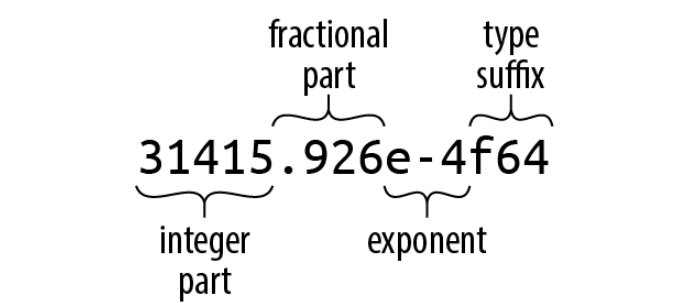
\includegraphics[width=0.8\textwidth]{../img/f3-1.png}
    \caption{浮点数字面量}
    \label{f3-1}
\end{figure}

整数部分之后的部分都是可选的,但小数部分、指数、或者类型后缀至少需要有一个,才能和整数字面量区分开。小数部分可以只有一个单独的小数点,因此\texttt{5.}是一个有效的浮点数。

如果一个浮点数字面量缺少类型后置,和处理整数一样,Rust会检查上下文来查看这个值是如何使用的。如果最后它发现两种浮点数类型都可以满足语义,那么它会默认选择\texttt{f64}。

为了实现类型推导,Rust把整数字面量和浮点数字面量区分为不同的种类:它从来不会把一个浮点数类型推断为整数类型,反之亦然。\hyperref[t3-9]{表3-9}展示了一下浮点数字面量的例子。

\begin{table}[htbp]
    \centering
    \caption{浮点数字面量的示例}
    \label{t3-9}
    \begin{tabular}{lll}
        \hline
        \textbf{字面量} & \textbf{类型} & \textbf{数值} \\
        \hline
        \texttt{-1.5625}    & 自动推断  & $-1\frac{9}{16}$  \\
        \rowcolor{tablecolor}
        \texttt{2.}         & 自动推断  & 2 \\
        \texttt{0.25}       & 自动推断  & $\frac{1}{4}$   \\
        \rowcolor{tablecolor}
        \texttt{1e4}        & 自动推断  & 10,000    \\
        \texttt{40f32}      & \texttt{f32}  & 40    \\
        \rowcolor{tablecolor}
        \texttt{9.109\_383\_56e-31f64} & \texttt{f64} & 大约是$9.10938356\times10^{-31}$ \\
    \end{tabular}
\end{table}

\texttt{f32}和\texttt{f64}类型还关联了IEEE要求的特殊常量值例如\texttt{INFINITY}、\texttt{NEG\_INFINITY}(负无穷)、\texttt{NAN}(非数值)、\texttt{MIN}和\texttt{MAX}(最小和最大的有限值):
\begin{minted}{Rust}
    assert!((-1. / f32::INFINITY).is_sign_negative());
    assert_eq!(-f32::MIN, f32::MAX);
\end{minted}
\texttt{f32}和\texttt{f64}类型提供了完整的数值计算的方法;例如,\texttt{2f64.sqrt()}是2的平凡根。还有一些示例:
\begin{minted}{Rust}
    assert_eq!(5f32.sqrt() * 5f32.sqrt(), 5.);  // 精确的5.0
    assert_eq!((-1.01f64).floor(), -2.0);
\end{minted}

再重复一次,方法调用的优先级高于前缀运算符,因此对负数调用方法时确保要用括号括起来。

\texttt{std::f32::consts}和\texttt{std::f64::consts}模块提供了常用的数学常数,例如\texttt{E}、\texttt{PI}、2的平方根。

当查找文档时,记得既有类型的文档,名称叫“\texttt{f32}(primitive type)”和“\texttt{f64}(primitive type)”,又有模块的文档,名称叫\texttt{std::f32}和\texttt{std::f64}。

和整数一样,在实际编码时通常你不需要写出浮点数字面量的类型后缀,但如果你要写,那么只需要指明变量和函数其中一个类型即可:
\begin{minted}{Rust}
    println!("{}", (2.0_f64).sqrt());
    println!("{}", f64::sqrt(2.0));
\end{minted}
和C和C++不同,Rust中几乎没有隐式类型转换。如果一个函数接收\texttt{f64}类型的参数,传递\texttt{i32}的值作为参数将是一个错误。事实上,Rust甚至不允许从\texttt{i16}到\texttt{i32}这样的隐式转换,尽管每一个\texttt{i16}值也都是一个合法的\texttt{i32}值。但你总是可以使用\texttt{as}运算符来进行\texttt{显式}转换:\texttt{i as f64},或者\texttt{x as i32}。

缺少隐式类型转换导致Rust的表达式可能会比C和C++中类似的表达式更加冗长。然而,隐式整数转换经常导致bug和安全漏洞。尤其是用来表示内存中某个东西的长度的整数,可能会导致意外的溢出。在我们的实践中,在Rust中显式写出类型转换可以提醒我们可能忽略的问题。

我们会在“\hyperref[cast]{类型转换}”一节中介绍转换的原理。

\section{布尔类型}

Rust的布尔类型\texttt{bool},只有两个值:\texttt{true}和\texttt{false}。比较运算符例如\texttt{==}和\texttt{<}会产生\texttt{bool}类型的结果:\texttt{2 < 5}的结果是\texttt{true}。

许多语言都很宽容,允许在需要布尔值的上下文中使用其他类型:C和C++隐式把字符、整数、浮点数和指针转换为布尔值,因此它们可以直接用作\texttt{if}或\texttt{while}语句的条件。Python还允许string、list、字典、甚至集合用作布尔值,如果不为空时视为true。然而Rust非常严格:像\texttt{if}和\texttt{while}这样的控制流的条件必须是\texttt{bool}表达式,短路求职运算符\texttt{\&\&}和\texttt{||}也是这样。你必须写\texttt{if x != 0 \{ ... \}},而不能写\texttt{if x \{ ... \}}。

Rust的\texttt{as}运算符可以把\texttt{bool}值转换为整数值:
\begin{minted}{Rust}
    assert_eq!(false as i32, 0);
    assert_eq!(true  as i32, 1);
\end{minted}

然而,\texttt{as}不能反过来把整数值转换为\texttt{bool}值。你必须显式写出比较运算例如\texttt{x != 0}。

尽管\texttt{bool}类型只需要单个比特来表示,Rust还是使用整个字节来表示\texttt{bool},因此你可以创建指向它的指针。


    \chapter{所有权与move}\label{ch04}

在内存管理方面,我们希望编程语言能够具备以下两个特点:
\begin{itemize}
    \item 我们希望内存能在我们想要释放的时候被及时释放。这样我们可以控制程序的内存消耗。
    \item 我们永远不希望使用一个指向已经被释放的对象的指针。这会导致未定义行为,进而导致崩溃和安全漏洞。
\end{itemize}

但这两点看起来似乎是相互矛盾的:释放一个还有指针指向的对象的内存必定会导致悬垂指针。几乎所有的主流编程语言都属于两个阵营之一,取决于它们放弃了哪一点:
\begin{itemize}
    \item “安全优先”的阵营使用垃圾回收来管理内存,自动释放那些没有指针指向的对象。这种做法通过将对象一直保持到没有指针指向来避免悬垂指针。几乎所有的现代语言都落入了这个阵营,包括Python、JavaScript、Ruby、Java、C\#、Haskell。

    但依赖垃圾回收意味着放弃控制对象被回收的精确时间。垃圾收集器通常都令人讨厌,并且理解为什么内存没有如你所料的被释放可能会是一个挑战。

    \item “控制优先”的阵营让你自己负责释放内存。程序的内存消耗完全由你控制,但如何避免悬垂指针成了你最大的问题。C和C++是这个阵营里仅有的主流语言。

    如果你从没犯过错,那说明你很厉害。但证据表明,你最终还是会犯错。指针的错误使用一直都是那些被报导的安全问题的罪魁祸首。
\end{itemize}

Rust旨在同时保证安全和性能,因此这两种阵营都是不可接受的。但如果兼顾两者很简单的话,早就有人做出来了。要想兼顾两者,必须从根本上作出改变。

Rust以一种令人惊讶的方式打破了这个死锁:严格限制程序使用指针的方法。这一章和接下来将专注于解释这些限制和为什么它们能解决问题。你常用的一些程序结构可能也不符合这些规则,你可能需要寻找替代方案。但这些限制的最终效果是给这种混乱带来了足够的秩序,以允许Rust在编译期检查你的程序是否能避免内存安全错误:悬垂指针、两次释放、使用未初始化的内存等。在运行时,你的指针只是简单的地址,就像在C和C++中一样。不同的是你的代码已经被证明是安全的。

这些规则也为Rust实现安全的并发编程奠定了基础。Rust精心设计的线程原语可以让这些保证内存安全的规则也能保证你的代码可以避免数据竞争。Rust程序中的一个bug不可能导致一个线程破坏另一个线程的数据进而导致在不相干的地方出现很难复现的错误。多线程代码中的不确定行为被那些专为它设计的特性——互斥锁、消息通道、原子类型等完全隔离,不会出现在正常的内存访问中。C和C++中的多线程代码臭名昭著,但Rust漂亮地解决了它。

即使有这些限制,你会发现它仍然可以足够灵活地处理几乎所有的任务,而它可以消除内存管理和并发bug的优势将证明你需要改变——你需要对自己的风格进行调整。这是Rust最大的赌注,也是它的核心和成功之处。本书的作者们看好Rust,正是因为我们在C和C++方面有丰富的经验。对我们来说,遵守Rust的规则不费吹灰之力。\footnote{译者注:此处原文:For us, Rust's deal is a no-brainer.}

Rust的规则可能和你在其他编程语言中看到的不同。了解怎么和它们一起工作并利用它们的优势,在我们看来是学习Rust的核心挑战。在这一章中,我们将首先展示相同的潜在问题如何在其他语言中导致问题,以此来深入了解Rust规则背后的逻辑和意图。之后,我们将详细解释Rust的规则、从概念和机制层面探究所有权的含义、如何在各种场景下追踪所有权的变化、以及一些为了提供更大的灵活性而打破这些规则的类型。

\section{所有权}

如果你读过很多C或C++的代码,你可能会看到过有注释说某个类的实例\emph{拥有(own)}某些它指向的其他对象。这一般意味着拥有者可以决定何时释放它拥有的对象:当拥有者被销毁时,它会销毁所有它拥有的对象。

例如,假设你写了如下C++代码:
\begin{minted}{Rust}
    std::string s = "frayed knot";
\end{minted}

字符串\texttt{s}在内存中的表示通常如\hyperref[f4-1]{图4-1}所示:
\begin{figure}
    \centering
    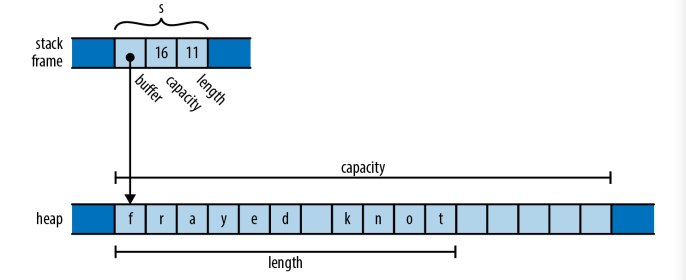
\includegraphics[width=0.8\textwidth]{../img/f4-1.png}
    \caption{一个栈上的C++ \texttt{std::string},指向它在堆上分配的内存}
    \label{f4-1}
\end{figure}

这里,实际上\texttt{std::string}对象本身总是只有3个字长,包括一个指向堆上分配的缓冲区的指针、缓冲区的最大容量(也就是在不重新分配缓冲区的情况下,能存储的最大文本长度),和已经持有的文本的长度。这些都是\texttt{std::string}的私有字段,使用者不能访问。

一个\texttt{std::string}拥有它的缓冲区,当程序销毁string时,它的析构函数会释放缓冲区。以前,一些C++库在多个\texttt{std::string}值之间共享单个缓冲区,使用一个引用计数来决定缓冲区什么时候应该被释放。较新版本的C++标准有效地排除了这种表示,所有现代的C++库都是用上图中的方式。

在这些场景中,人们普遍认为尽管其他代码创建这些被拥有的内存的指针是没问题的,但这些代码有责任确保在所有者决定销毁它拥有的对象之前所有的这种指针都已消失。你可以创建一个指向\texttt{std::string}的缓冲区的指针,但当string被销毁后,你的指针就无效了,你必须自己保证不再使用它。拥有者决定所拥有对象的生命周期,所有其他的对象必须尊重它的决定。

我们在这里使用\texttt{std::string}做为例子展示了C++中的所有权是什么样子的:它只是一个标准库普遍遵守的规范。然而即使语言鼓励你也遵守相似的实践,但如何设计你自己的类型最终还是取决于你。

但在Rust中,所有权的概念被内建在语言之中,并且通过编译期检查确保强制执行。每个值都只有一个决定它生命周期的所有者。当所有者被释放——Rust中的术语叫\emph{dropped}——它拥有的值也会被dropped。这些规则的目的是让你可以通过检查代码很容易的查明某个值的生命周期,并给你系统语言应有的控制生命周期的能力。

一个变量拥有它的值。当控制流离开了变量声明的语法块,变量会被drop,因此它的值也会随之一起drop。例如:
\begin{minted}{Rust}
    fn print_padovan() {
        let mut padovan = vec![1,1,1];  // 在这里分配
        for i in 3..10 {
            let next = padovan[i-3] + padovan[i-2];
            padovan.push(next);
        }
        println!("P(1..10) = {:?}", padovan);
    }
\end{minted}

变量\texttt{padovan}的类型是\texttt{Vec<i32>},一个32位整数的vector。在内存中,\texttt{padovan}看起来将类似于\hyperref[f4-2]{图4-2}。

\begin{figure}[htbp]
    \centering
    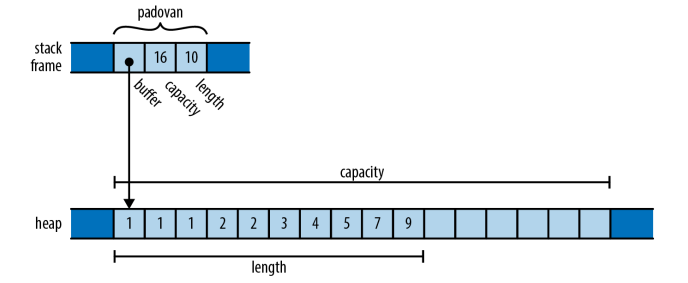
\includegraphics[width=0.8\textwidth]{../img/f4-2.png}
    \caption{栈上的\texttt{Vec<i32>},指向它在堆上的缓冲区}
    \label{f4-2}
\end{figure}

这和我们之前展示的C++的\texttt{std::string}非常像,除了缓冲区里的元素是32位整数,而不是字符。注意存储\texttt{padovan}的指针、容量和长度的字都在\texttt{print\_padovan}函数的栈帧中,只有vector的缓冲区是在堆上分配的。

和之前展示的string \texttt{s}一样,vector拥有它用来存储元素的缓冲区。当变量\texttt{padovan}在函数结尾处离开作用域时,程序会drop这个vector。因为vector拥有它的缓冲区,缓冲区也会随之drop。

Rust的\texttt{Box}类型是另一个所有权的例子。\texttt{Box<T>}是一个指针,指向一个存储在堆上的类型\texttt{T}的值,调用\texttt{Box::new(v)}会在堆上分配一些空间,把值\texttt{v}移动进去,然后返回一个\texttt{Box}指向堆上的空间。因为一个\texttt{Box}拥有它所指向的空间,当\texttt{Box}被drop的时候,堆上的空间也会被释放。

例如,你可以像这样在堆上分配一个元组:
\begin{minted}{Rust}
    {
        let point = Box::new((0.625, 0.5));     // point在这里分配
        let label = format!("{:?}", point);     // label在这里分配
        assert_eq!(label, "(0.625, 0.5)");
    }                                           // point和label都在这里drop
\end{minted}

当程序调用\texttt{Box::new}时,它会在堆上为一个由两个\texttt{f64}值组成的元组分配空间,把它的参数\texttt{(0.625, 0.5)}移动进去,然后返回一个指向它的指针。当控制流到达\texttt{assert\_eq!}的调用时,栈帧如\hyperref[f4-3]{图4-3}所示。

\begin{figure}[htbp]
    \centering
    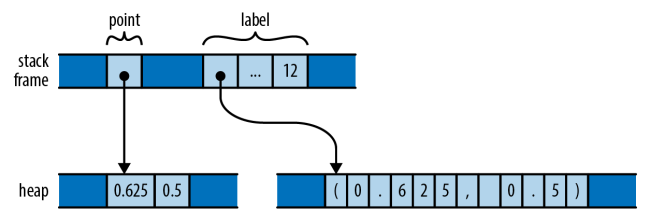
\includegraphics[width=0.8\textwidth]{../img/f4-3.png}
    \caption{两个本地变量,每个都拥有堆上的一块内存}
    \label{f4-3}
\end{figure}

栈帧本身存储了变量\texttt{point}和\texttt{label},每一个变量都指向自己拥有的堆上的内存。当它们被drop时,它们拥有的内存也随之释放。

与变量拥有它们的值类似,结构体拥有它们的字段,元组、数组、vector拥有它们的元素。

\begin{minted}{Rust}
    struct Person { name: String, birth: i32 }
    let mut composers = Vec::new();
    composers.push(Person { name: "Palestrina".to_string(),
                            birth: 1525 });
    composers.push(Person { name: "Dowland".to_string(),
                            birth: 1563 });
    composers.push(Person { name: "Lully".to_string(),
                            birth: 1632 });
    for composer in &composers {
        println!("{}, born {}", composer.name, composer.birth);
    }
\end{minted}

这里,\texttt{composers}是一个\texttt{Vec<Person>}:一个结构体的vector,每个结构体有一个字符串和数字。在内存中,\texttt{composers}的最终结果如\hyperref[f4-4]{图4-4}所示。

\begin{figure}[htbp]
    \centering
    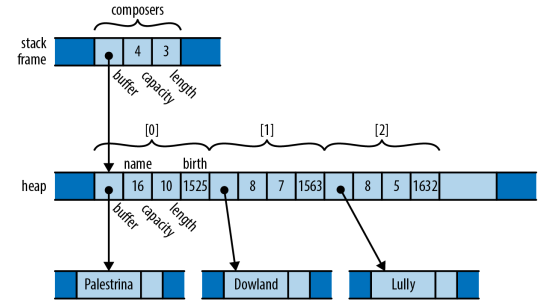
\includegraphics[width=0.8\textwidth]{../img/f4-4.png}
    \caption{一个更复杂的所有权树}
    \label{f4-4}
\end{figure}

这里有很多的所有权关系,但每一个都很直观:\texttt{composers}拥有一个vector,vector拥有它的元素,每一个元素是一个\texttt{Person}结构体;每个结构体拥有它的字段;其中的字符串字段拥有它的文本。当控制流离开了\texttt{composers}声明的作用域,程序会drop它的值,同时drop它拥有的所有内容。如果这里还有其他类型的集合,例如\texttt{HashMap}、\texttt{BTreeSet},那么过程也是一样的。

到这里,让我们退后一步并思考我们到目前为止展示的所有权关系。每个值都只有一个所有者,这样很容易决定什么时候drop这个值。但单个值可能拥有很多其他值:例如,vector \texttt{composers}拥有它的所有元素。这些元素也可能反过来拥有其他值:\texttt{composers}的每个元素拥有一个字符串,字符串又拥有它的文本。

所有者和它们拥有的值组成了\emph{树}:值的拥有者是它的父结点,值拥有的值是它的孩子结点。每棵树的根结点是一个变量;当这个变量离开作用域时,整个树都会随之销毁。我们可以在\texttt{composers}的图中看到这样一棵所有权的树:它不是搜索树数据结构意义上的“树”、也不是DOM元素组成的HTML文档树。相反,我们有一个由混合类型构建的树,Rust的单一所有者规则禁止任何可能使布局变得比树更复杂的连接操作。Rust程序中的每个值都是树中的一个结点,树的根就是变量。

Rust程序通常完全不需要像C和C++程序中使用\texttt{free}和\texttt{delete}一样显式drop值。Rust\\
中drop值的方式是将它从所有权树移除:当离开作用域时、或者从vector中删除元素时、或者类似的情况。这时,Rust保证值会和它拥有的所有值一起被drop掉。

在某种意义上,Rust不如其他语言强大:每个其他的编程语言都允许你在对象之间构建任意的关系图,这些对象以你认为合适的方式互相指向。但正因为Rust不够强大,所以它才可以对你的程序进行更强大的分析。Rust的安全保证可以实现的原因就是你的代码中可能出现的所有权关系更加容易处理。这是我们之前提到的Rust的“激进赌注”的一部分:Rust声称,在实践中,解决问题时通常有足够的灵活性来保证至少有一些完美的解决方案可以在语言强加的限制范围内实现。

也就是说,我们到目前为止解释的所有权的概念太过死板以至于很难使用。Rust在以下几个方面扩展了这个简单的想法:
\begin{itemize}
    \item 你可以将值从一个所有者移动到另一个所有者。这允许你构建、更改、拆除所有权树。
    \item 很简单的类型例如整数、浮点数和字符被所有权规则排除在外。它们被称为\texttt{Copy}类型。
    \item 标准库提供了引用计数的指针类型\texttt{Rc}和\texttt{Arc},它们允许值在一定的限制下可以有多个所有者。
    \item 你可以“借用一个值的引用”,引用是生命周期受限的非占有的指针。
\end{itemize}

这些策略中的每一条都改善了所有权模型的灵活性,同时仍然坚持Rust的承诺。我们将依次介绍它们,引用将在下一章介绍。

\section{move}
在Rust里对大多数类型来说,赋值给变量、把值传给函数、或者从函数返回值并不会拷贝这个值:它们只会\emph{move}它。源对象放弃了值的所有权,把所有权转移给了目的对象,同时源对象变为未初始化的状态;此时目的对象控制值的生命周期。Rust程序一次一个值、一次move一个地构建和拆除复杂的结构。

你可能会很惊讶Rust改变了这些基础操作的含义。确实赋值操作很早之前就已经有了明确的含义。然而,如果你仔细观察过不同的语言是怎么处理赋值操作的,你就会发现不同语言的处理方式有很大差别。这种差别也让我们能更容易的看出Rust的选择的含义和结果。

考虑下面的Python代码:
\begin{minted}{python}
    s = ['udon', 'ramen', 'soba']
    t = s
    u = s
\end{minted}

每一个Python对象都有一个引用计数,用来追踪当前有多少个值指向它。因此在对\texttt{s}赋值以后,程序的状态如\hyperref[f4-5]{图4-5}所示(注意有一些内容被省略了)。

\begin{figure}[htbp]
    \centering
    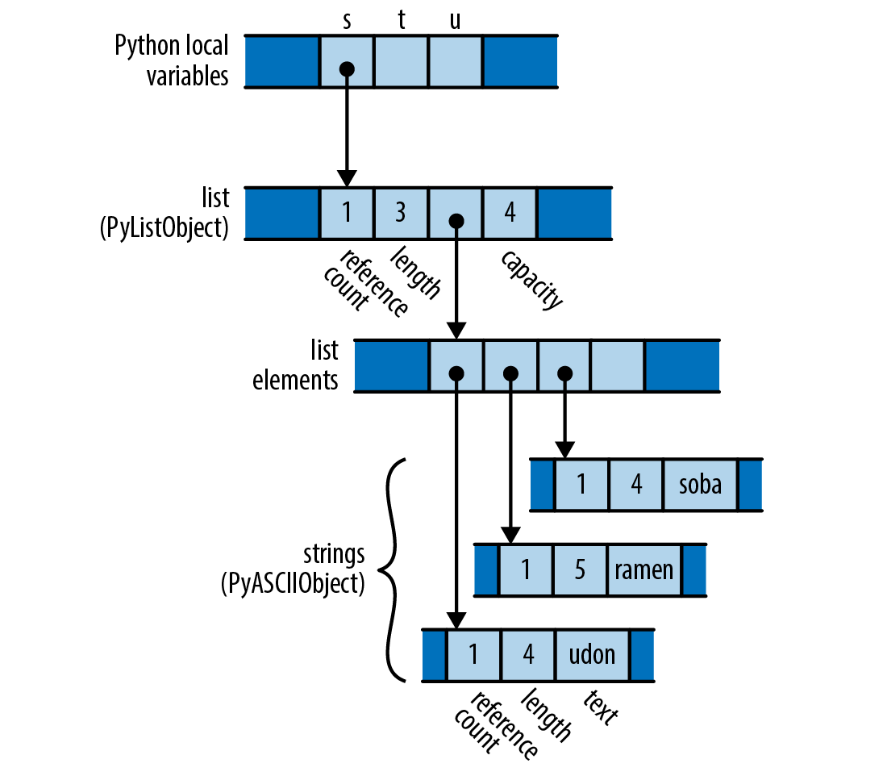
\includegraphics[width=0.9\textwidth]{../img/f4-5.png}
    \caption{Python如何在内存中表示一个字符串的列表}
    \label{f4-5}
\end{figure}

因为只有\texttt{s}指向列表,所以列表的引用计数是1;因为列表是唯一指向那些字符串的对象,所以每个字符串的引用计数也是1。

当程序执行到\texttt{t}和\texttt{u}的赋值时会发生什么?Python把赋值操作简单实现为让目标变量也指向源变量指向的对象,然后增加对象的引用计数。因此,这段程序的最终状态如\hyperref[f4-6]{图4-6}所示:
\begin{figure}[htbp]
    \centering
    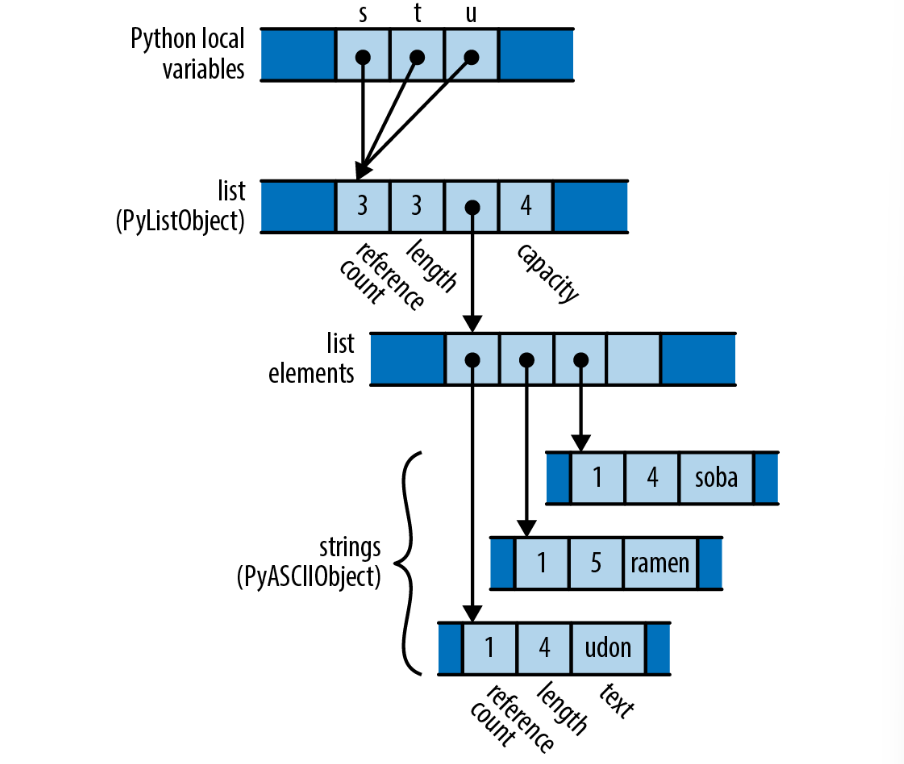
\includegraphics[width=0.8\textwidth]{../img/f4-6.png}
    \caption{在Python里把\texttt{s}赋值给\texttt{t}和\texttt{u}的结果}
    \label{f4-6}
\end{figure}

Python拷贝了\texttt{s}的指针,并赋给了\texttt{t}和\texttt{u},然后把列表的引用计数更新为3。Python中的赋值开销很低,但因为它创建了新的指向对象的引用,我们必须维护引用计数来知道我们什么时候可以释放值。

现在考虑下面类似的C++代码:
\begin{minted}{C++}
    using namespace std;
    vector<string> s = { "udon", "ramen", "soba" };
    vector<string> t = s;
    vector<string> u = s;
\end{minted}

一开始\texttt{s}的值在内存中如\hyperref[f4-7]{图4-7}所示。

\begin{figure}[htbp]
    \centering
    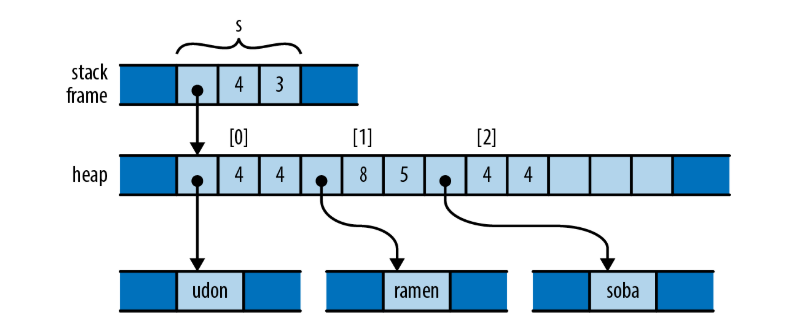
\includegraphics[width=0.8\textwidth]{../img/f4-7.png}
    \caption{C++里一个字符串的vector在内存中的表示}
    \label{f4-7}
\end{figure}

当把\texttt{s}赋值给\texttt{t}和\texttt{u}时会发生什么呢?在C++里赋值一个\texttt{std::vector}会产生一份这个vector的拷贝;\texttt{std::string}的行为类似。因此当程序到达末尾时,它实际上有3个vector和\\
9个字符串(\hyperref[f4-8]{图4-8})。

\begin{figure}[htbp]
    \centering
    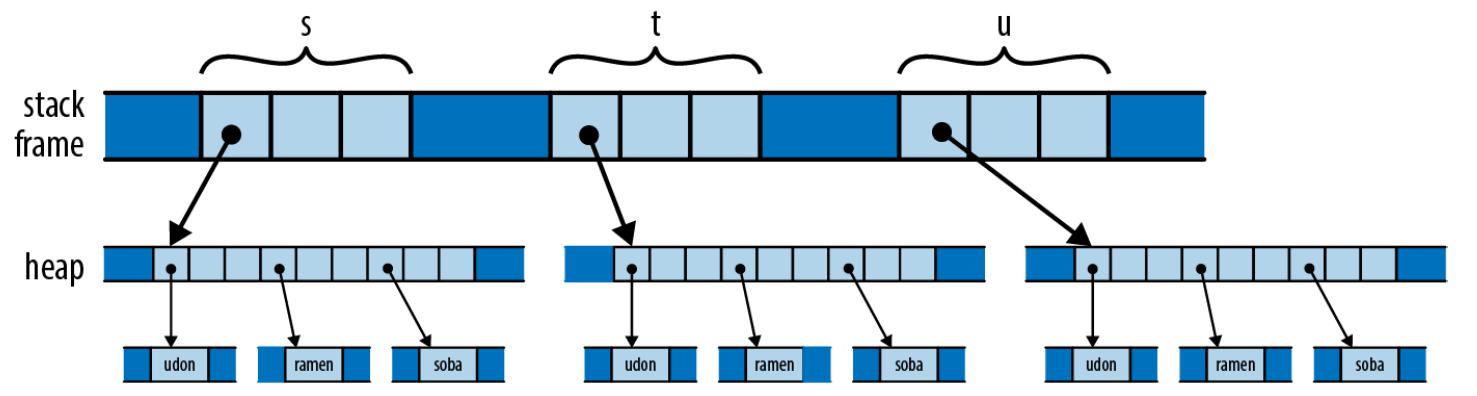
\includegraphics[width=0.8\textwidth]{../img/f4-8.png}
    \caption{在C++里把\texttt{s}赋值给\texttt{t}和\texttt{u}的结果}
    \label{f4-8}
\end{figure}

根据值的不同,C++里的赋值可能会消耗任意数量的内存和处理器时间。然而,它的优势是,程序可以很容易的决定何时释放这些内存:当变量离开作用域时,所有这里分配的内存都会被自动释放。

某种意义上,C++和Python选择了相反的策略:Python里赋值操作开销很小,但引用计数(通用一点的说法,垃圾回收)开销很大。C++保持了内存的所有权都很清楚,但赋值时会执行对象的深拷贝导致开销很大。C++程序员通常不太热衷于这种选择:深拷贝可能开销很大,通常会有更好的替代方法。

那么Rust中的类似程序会怎么做呢?代码如下:
\begin{minted}{Rust}
    let s = vec!["udon".to_string(), "ramen".to_string, "soba".to_string()];
    let t = s;
    let u = s;
\end{minted}

类似于C和C++,Rust把字符串字面量例如\texttt{"udon"}存储在只读内存中,因此,为了更清楚地与C++和Python的例子进行对比,我们调用了\texttt{to\_string}来获得在堆上分配的\texttt{String}值。

在\texttt{s}的初始化之后,因为Rust和C++有相似的vector和string表示,所以看起来和C++中的情况很像(\hyperref[f4-9]{图4-9})。

\begin{figure}[htbp]
    \centering
    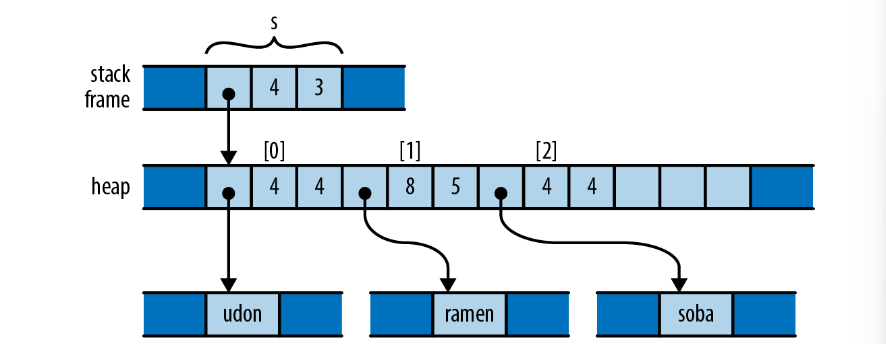
\includegraphics[width=0.8\textwidth]{../img/f4-9.png}
    \caption{Rust中一个字符串的vector在内存中的表示}
    \label{f4-9}
\end{figure}

但回想一下,Rust里大多数类型的赋值操作都是把值从源对象\emph{移动}到目的对象,然后源对象变为未初始化的状态。因此\texttt{t}初始化完之后,程序的内存状态如\hyperref[f4-10]{图4-10}所示。

\begin{figure}[htbp]
    \centering
    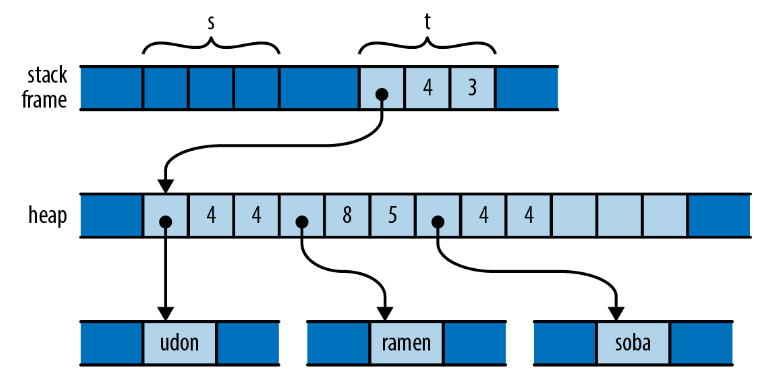
\includegraphics[width=0.8\textwidth]{../img/f4-10.png}
    \caption{Rust里把\texttt{s}赋值给\texttt{t}之后的结果}
    \label{f4-10}
\end{figure}

这里发生了什么?赋值语句\texttt{let t = s;}把vector的三个字段从\texttt{s}移动到了\texttt{t};现在\texttt{t}拥有了这个vector。vector的元素则仍待在原来的位置,string的位置也没有发生变化。每一个值都只有一个所有者,尽管所有者已经变了。不需要调整引用计数,并且编译器现在把\texttt{s}视作未初始化的状态。

因此当我们到达\texttt{let u = s;}时会发生什么呢?这将会把\texttt{s}赋值给\texttt{u}。Rust禁止使用未初始化的值,所以编译器会报如下错误:
\begin{minted}{text}
    error[E0382]: use of moved value: `s`
      |
    7 |     let s = vec!["udon".to_string(), "ramen".to_string(), "soba".to_string()];
      |         - move occurs because `s` has type `Vec<String>`,
      |           which does not implement the `Copy` trait
    8 |     let t = s;
      |             - value moved here
    9 |     let u = s;
      |             ^ value used after move
\end{minted}

考虑Rust在这里使用move的结果。类似于Python,赋值操作开销很小,程序简单地把vector的三个字长的头部从一个点移动到了另一个点。但和C++类似,所有权总是很清晰:程序不需要引用计数或者垃圾回收来判断什么时候释放vector的元素和string的内容。

而为此付出的代价是如果赋值时想要的是拷贝操作那么必须显式写出。如果你想要最后和C++程序一样的状态,也就是每个变量都有独立的拷贝,那么必须调用vector的\texttt{clone}方法,它会对vector和它的元素执行深拷贝:
\begin{minted}{Rust}
    let s = vec!["udon".to_string(), "ramen".to_string(), "soba".to_string()];
    let t = s.clone();
    let u = s.clone();
\end{minted}

你也可以通过Rust的引用计数指针类型复现Python代码的行为,我们将在\hyperref[rc]{Rc和Arc:共享所有权}这一节中简要介绍这一点。

\subsection{更多move的操作}

在我们上面展示的初始化例子中,都是在使用\texttt{let}语句引入变量的同时把值赋给它们。赋值给一个变量将与此有细微的不同,如果你把值移动进一个已经被初始化的变量,Rust会drop变量之前的值。例如:
\begin{minted}{Rust}
    let mut s = "Govinda".to_string();
    s = "Siddhartha".to_string();   // 值"Govinda"在这里drop
\end{minted}

在这段代码中,当程序把\texttt{"Siddhartha"}赋值给\texttt{s}时,它之前的值\texttt{"Govinda"}首先被drop掉。但考虑下面的代码:
\begin{minted}{Rust}
    let mut s = "Govinda".to_string();
    let t = s;
    s = "Siddhartha".to_string();   // 这里不会drop任何内容
\end{minted}

这一次,\texttt{t}拿走了\texttt{s}中原本的字符串的所有权,因此当我们给\texttt{s}赋值时,它是未初始化的。在这种场景下,不会发生drop。

我们在这里使用初始化和赋值的例子是因为它们足够简单,但Rust在几乎所有场景下都使用move。向函数传参会把所有权移动给函数的参数;从函数返回值会把所有权移动给调用者;创建一个元组会把值移动给元组,等等。

你现在可能对我们之前章节给出的例子中到底发生了什么有了更深入的理解。例如,当我们构建作曲家的vector时,我们写了:
\begin{minted}{Rust}
    struct Person { name: String, birth: i32 }

    let mut composers = Vec::new();
    composers.push(Person { name: "Palestrina".to_string(), 
                            birth: 1525 });
\end{minted}

这段代码展示了除了初始化和赋值之外,move发生的几个场景:
\begin{flushleft}
    \emph{从函数返回值}
\end{flushleft}

\hangparagraph{调用\texttt{Vec::new()}会创建一个新的vector并返回,返回的并不是指向vector的指针,而是vector本身:它的所有权从\texttt{Vec::new}移动到了变量\texttt{composers}。类似的,\texttt{to\_string}调用返回了一个新的\texttt{String}实例。}

\begin{flushleft}
    \emph{构造新的值}
\end{flushleft}

\hangparagraph{新的\texttt{Person}结构体的\texttt{name}字段被\texttt{to\_string}的返回值初始化。结构体获得了这个字符串的所有权。}

\begin{flushleft}
    \emph{向函数传递值}
\end{flushleft}

\hangparagraph{整个\texttt{Person}结构体,而不是指向它的指针,被传递给vector的\texttt{push}方法,这个方法将值移动到了结构体的尾部。vector获得了\texttt{Person}的所有权,因此也变成了name \texttt{String}的间接所有者。}

像这样移动值可能听起来并不是很高效,但有两件事需要记住。第一,move只作用于恰当的值,而不作用于它们拥有的堆存储。对于vector和string来说,\emph{恰当的值}是它们三个字长的头部,潜在的很多元素的数组和文本缓冲区仍然停留在堆中原本的位置。第二,Rust编译器的代码生成部分擅长“看穿”所有这些move;在实践中,机器码通常会直接把值存储到它最终的位置。

\subsection{move和控制流}
之前的例子中的控制流都很简单,move会如何影响更复杂的代码呢?通用的原则是,如果一个变量的值被移动走并且从此之后没有再被赋予一个新的值,那么它被认为是未初始化的。例如,如果一个变量在\texttt{if}表达式的条件判断之后还是有值的,那我们在两个分支中都可以使用它:
\begin{minted}{Rust}
    let x = vec![10, 20, 30];
    if c {
        f(x);   // ... 在这里移动x的值是ok的
    } else {
        g(x);   // ... 在这里移动x的值也是ok的
    }
    h(x);   // 错误:如何任何一个分支使用了x,那么x在此处将是未初始化的
\end{minted}

出于类似的原因,在循环里移动一个变量的值是禁止的:
\begin{minted}{Rust}
    let x = vec![10, 20, 30];
    while f() {
        g(x);   // 错误:x会在第一次迭代时被移动
                // 第二次迭代时就是未初始化状态 
    }
\end{minted}

也就是说,我们需要在每次迭代里都重新赋予它一个新值:
\begin{minted}{Rust}
    let mut x = vec![10, 20, 30];
    while f() {
        g(x);       // 移动x的值
        x = h();    // 给x一个新值
    }
\end{minted}

\subsection{move和索引}

我们已经提到过move会将源对象设置为未初始化状态,目的对象会获得值的所有权。但并不是每一种值的所有者都可以设置为未初始化状态。例如,考虑下面的代码:
\begin{minted}{Rust}
    // 创建一个string的vector:"101", "102", ... "105"
    let mut v = Vec::new();
    for i in 101 .. 106 {
        v.push(i.to_string());
    }

    // 从vector中取出随机的元素
    let third = v[2];   // 错误:不能移动Vec的索引
    let fifth = v[4];   // 这里也是一样
\end{minted}

如果想让这段代码工作,Rust需要记住这个vector的第3和第5个元素变成了未初始化状态,然后一直追踪这些信息直到这个vector被drop。在一般情况下,vector需要携带额外的信息来指示哪些元素还可用,哪些变为了未初始化。显然这不是一门系统编程语言应该有的行为;一个vector应该只是一个vector。事实上,Rust会报错拒绝上面的代码:
\begin{minted}{text}
    error[E0507]: cannot move out of index of `Vec<String>`
       |
    14 |     let third = v[2];
       |                 ^^^^
       |                 |
       |                 move occurs because value has type `String`,
       |                 which does not implement the `Copy` trait
       |                 help: consider borrowing here: `&v[2]`
\end{minted}

移动到\texttt{fifth}的语句也会报类似的错误。在这些错误信息中,Rust建议使用引用,这样就可以在不移动的情况下访问元素。这通常是你想要的。但如果我们真的想从vector中移出一个元素呢?你需要找到一些不违反类型限制的方法来做这件事。这里有三种方法:
\begin{minted}{Rust}
    // 创建一个string的vector:"101", "102", ... "105"
    let mut v = Vec::new();
    for i in 101 .. 106 {
        v.push(i.to_string());
    }

    // 1. 弹出vector尾部的元素
    let fifth = v.pop().expect("vector empty!");
    assert_eq!(fifth, "105");

    // 2. 移出给定位置的元素,并把最后一个元素移动过来:
    let second = v.swap_remove(1);
    assert_eq!(second, "102");

    // 3. 用另一个值和我们想移出的值交换
    let third = std::mem::replace(&mut v[2], "substitute".to_string());
    assert_eq!(third, "103");

    // 让我们看看vector中还剩下什么。
    assert_eq!(v, vec!["101", "104", "substitute"]);
\end{minted}

这三种方法都从vector中移出一个元素,但仍然保证vector处于没有空隙的状态,可能长度还会变小。

像\texttt{Vec}这样的集合类型也提供方法通过循环消费它们的所有元素:
\begin{minted}{Rust}
    let v = vec!["liberté".to_string(),
                 "égalité".to_string(),
                 "fraternité".to_string()];
    for mut s in v {
        s.push('!');
        println!("{}", s);
    }
\end{minted}

当直接把vector传给循环时,例如\texttt{for ... in v},这会把\texttt{v}中的所有元素\emph{移出}vector,然后\texttt{v}变为未初始化。\texttt{for}循环内部的机制会获取vector的所有权,然后把它分解为若干元素。每一次迭代时,循环都会把一个元素移动到变量\texttt{s}。因为\texttt{s}现在拥有这个字符串,所以我们可以在循环里修改它,然后再打印。因为vector本身不再对代码可见,所以在循环的过程中当它部分为空时没有任何东西可以观测到它。

如果你确实发现你需要从所有者中移出一个编译器无法追踪的值,你可以考虑将所有者的类型改为可以动态追踪是否有值的类型。例如,这里有一个之前示例的变体:
\begin{minted}{Rust}
    struct Person { name: Option<String>, birth: i32 }

    let mut composers = Vec::new();
    composers.push(Person { name: Some("Palestrina".to_string()),
                            birth: 1525 });
\end{minted}

你不能这样做:
\begin{minted}{Rust}
    let first_name = composers[0].name;
\end{minted}

这只会和犯和之前一样的“不能移出索引”的错误。但因为你把\texttt{name}字段的类型从\texttt{String}改为了\texttt{Option<String>},这意味着\texttt{None}是这个字段的一个合法的取值,因此下面的代码可以生效:
\begin{minted}{Rust}
    let first_name = std::mem::replace(&mut composers[0].name, None);
    assert_eq!(first_name, Some("Palestrina".to_string()));
    assert_eq!(composers[0].name, None);
\end{minted}

\texttt{replace}调用移出了\texttt{composers[0].name}的值,留下了一个\texttt{None},并把原本的值的所有权传递给了调用者。事实上,这种使用\texttt{Option}的方法非常普遍,所以这个类型提供了一个\texttt{take}方法来实现这个特殊的用途。你可以使用下面的代码更清晰地完成上述操作:
\begin{minted}{Rust}
    let first_name = composers[0].name.take();
\end{minted}
这里的\texttt{take}调用和之前的\texttt{replace}调用有相同的效果。

\section{Copy类型:move的例外}\label{copy}
到目前为止我们的例子涉及vector、string、和其他可能潜在地使用大量内存并且拷贝开销很大的类型。move保证了这些类型的所有权的明晰、也保证了赋值的开销很小。但对于简单类型例如整数或字符,这种谨慎的处理方式事实上并不是必须的。

让我们比较一下赋值一个\texttt{String}和赋值一个\texttt{i32}值时内存中会发生什么:
\begin{minted}{Rust}
    let string1 = "somnambulance".to_string();
    let string2 = string1;

    let num1: i32 = 36;
    let num2 = num1;
\end{minted}

运行完这段代码后,内存布局如\hyperref[f4-11]{图4-11}所示。
\begin{figure}[htbp]
    \centering
    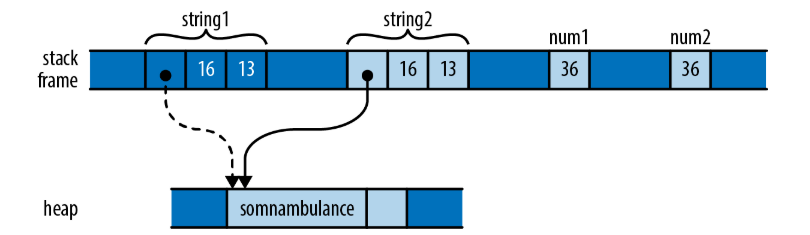
\includegraphics[width=0.9\textwidth]{../img/f4-11.png}
    \caption{赋值\texttt{String}会移动它,而赋值\texttt{i32}会拷贝它}
    \label{f4-11}
\end{figure}

类似于之前的vector,赋值会把\texttt{string1}\emph{移动}到\texttt{string2},这样我们就不会得到两个负责释放同一个缓冲区的字符串。然而,\texttt{num1}和\texttt{num2}的情况与此不同。\texttt{i32}只是在内存中的一种位模式,它并不拥有任何堆上的资源、也不依赖任何它本身所占的字节之外的东西。此时如果我们把它的位都移动给\texttt{num2},我们就得到了一个和\texttt{num1}完全互相独立的拷贝。

移动一个值会导致源对象变为未初始化。但是尽管把\texttt{string1}视为无值是一个基本的目的,但如果对\texttt{num1}也这么做是毫无意义的,继续使用\texttt{num1}不会导致任何危害。move的优势在这里并不适用,反而变得不够便捷。

之前我们谨慎的说过\emph{大多数}类型会被移动,现在我们来到了例外的情况,也就是Rust称之为\texttt{Copy type}的类型。赋予一个\texttt{Copy}类型的值会拷贝它,而不是移动它。源对象仍然保持初始化状态和可用性,它的值不会发生改变。向函数和构造器传递\texttt{Copy}类型也类似。

标准的\texttt{Copy}类型包括所有的机器整数和浮点数类型、\texttt{char}和\texttt{bool}类型,以及少数其他类型。\texttt{Copy}类型的元组或者固定大小的数组也是\texttt{Copy}类型。

只有简单的逐位拷贝的类型才可以是\texttt{Copy}类型。正如我们解释过的,\texttt{String}不是\texttt{Copy}类型,因为它拥有一个在堆上分配的缓冲区;与此类似,\texttt{Box<T>}也不是\texttt{Copy}类型,它拥有一个堆上分配的对象;代表操作系统中文件句柄的\texttt{File}类型,也不是\texttt{Copy}类型,赋值这样一个值意味着向操作系统请求另一个文件句柄。类似的,表示一个互斥锁的\texttt{MutexGuard}类型,也不是\texttt{Copy}类型,拷贝这个类型没有任何意义,因为在一个时间点只有一个线程可以持有锁。

根据经验,任何在drop时要做一些特殊事情的类型不可能是\texttt{Copy}类型:一个\texttt{Vec}需要释放它的内存,一个\texttt{File}需要关闭它的文件句柄,一个\texttt{MutexGuard}需要释放它的锁,等等。对这些类型逐位拷贝会导致搞不清它们中的哪一个要负责释放原始的资源。

自定义的类型呢?默认情况下,\texttt{struct}和\texttt{enum}不是\texttt{Copy}类型:
\begin{minted}{Rust}
    struct Label { number: u32 }
    fn print(l: Label) { println!("STAMP: {}", l.number); }

    let l = Label { number: 3 };
    print(l);
    println!("My label number is: {}", l.number);
\end{minted}

这不能通过编译,Rust会报错:
\begin{minted}{text}
    error: borrow of moved value: `l`
       |
    10 |     let l = Label { number: 3 };
       |         - move occurs because `l` has type `main::Label`,
       |           which does not implement the `Copy` trait
    11 |     print(l);
       |           - value moved here
    12 |     println!("My label number is: {}", l.number);
       |                                        ^^^^^^^^
       |                  value borrowed here after move
\end{minted}

因为\texttt{Label}不是\texttt{Copy}类型,将它传递给\texttt{print}会把值的所有权移动给\texttt{print}函数的参数,在函数返回时会drop掉值。但这非常愚蠢,一个\texttt{Label}只是一个\texttt{u32}套壳。没有理由将\texttt{l}传递给\texttt{print}时应该移动值。

但用户自定义类型只是默认不是\texttt{Copy}类型。如果你的结构体的所有字段都是\texttt{Copy}类型,那么你可以通过在定义上方加上属性\texttt{\#[derive(Copy, Clone)]}来把它变为\texttt{Copy}类型,像这样:
\begin{minted}{Rust}
    #[derive(Copy, Clone)]
    struct Label { number: u32 }
\end{minted}

这样修改之后,上面的代码就可以通过编译了。然而,如果我们用不是\texttt{Copy}类型的字段来修改这个类型的话,也不能通过编译。假设我们要编译下面的代码:
\begin{minted}{Rust}
    #[derive(Copy, Clone)]
    struct StringLabel { name: String }
\end{minted}

它会报这样的错误:
\begin{minted}{text}
    error[E0204]: the trait `Copy` may not be implemented for this type
     --> ownership_string_label.rs:7:10
      |
    7 | #[derive(Copy, Clone)]
      |          ^^^^
    8 | struct StringLabel { name: String }
      |                      ------------ this field does not implement `Copy`
\end{minted}

为什么不默认把用户自定义类型设置为\texttt{Copy}类型?一个类型是否是\texttt{Copy}类型对接下来的代码如何使用它有巨大的影响:\texttt{Copy}类型更加的灵活,因为赋值和相关的操作不会导致源对象变得未初始化。但对于类型的实现者来说,恰恰相反:\texttt{Copy}类型所能包含的类型十分有限,而非\texttt{Copy}类型可以使用堆上的内存并且拥有自己的资源。因此将一个类型标记为\texttt{Copy}代表着实现者的一个承诺:如果之后它必须要修改为非\texttt{Copy}类型,很多使用它的代码都需要修改。

虽然C++允许你重载赋值运算符和自定义拷贝和移动构造函数,但Rust不允许这种自定义。在Rust里,所有的移动都是逐字节的浅拷贝,同时把源对象设置为未初始化。拷贝与此类似,除了源对象仍然是初始化过的状态。这确实意味着C++类可以提供Rust类所不能提供的方便接口:看起来普通的代码会隐式的调整引用计数、推迟开销很大的拷贝操作、或者使用其它复杂的实现技巧。

但C++中的这种灵活性会导致基本操作例如赋值、传参、返回值变得不可预料。例如,这一章之前的部分我们展示过在C++里把一个变量赋给另一个可能会需要任意数量的内存和处理器时间。Rust的原则之一就是开销对程序员来说必须是明显的。基本的操作必须保持简单。潜在的开销很大的操作必须是显式的,例如在更早的例子中调用\texttt{clone}来获取vector和它包含的string的深拷贝。

在这一节中,我们谈到了术语\texttt{Copy}和\texttt{Clone},模糊地将它们视作类型具有的特征。事实上,它们是\texttt{trait}的示例,它是Rust的一个开发的工具,你可以通过它根据类型能做什么对类型进行分类。我们将在\hyperref[ch11]{第11章}中讨论一般性的trait,在\hyperref[ch13]{第13章}中专门讨论\texttt{Copy}和\texttt{Clone}。

\section{Rc和Arc:共享所有权}\label{rc}

尽管典型的Rust代码中几乎所有的值都只有一个所有者,但在一些情况下,很难让每个值的所有者都有你想要的生命周期,这时你可能会希望值一直保持有效,直到每一个所有者都使用完它。对于这种情况,Rust提供了引用计数类型\texttt{Rc}和\texttt{Arc}。正如你对Rust的期待一样,它们是安全的:你不可能忘记调整引用计数、创建其它指向它的指针、或者出现其他使用C++的引用计数指针类型时可能出现的问题。

\texttt{Rc}和\texttt{Arc}类型非常相似,它们唯一的不同之处在于\texttt{Arc}可以直接安全地在线程之间共享——名称\texttt{Arc}是\emph{原子引用计数}的缩写——\texttt{Rc}则使用更快一些的非线程安全代码来更新引用计数。如果你不需要在线程之间共享指针,那就没有必要承担\texttt{Arc}的性能损失,所以你应该使用\texttt{Rc};Rust会阻止你无意间在线程之间传递\texttt{Rc}。这两种类型在其他方面都是等价的,因此在本节的剩余部分,我们将只讨论\texttt{Rc}。

之前我们曾经展示过Python使用引用计数来管理值的生存周期。你可以使用\texttt{Rc}来在Rust中实现相似的效果。考虑下面的代码:
\begin{minted}{Rust}
    use std::rc::Rc;

    // Rust可以推断出所有这些类型,写出来是为了更清楚
    let s: Rc<String> = Rc::new("shirataki".to_string());
    let t: Rc<String> = s.clone();
    let u: Rc<String> = s.clone();
\end{minted}

对于任意类型\texttt{T},一个\texttt{Rc<T>}值是一个指向在堆上分配的\texttt{T}类型值的指针,同时还附有一个引用计数。克隆一个\texttt{Rc<T>}类型的值并不意味着拷贝\texttt{T},它只是简单的创建另一个指向它的指针,并且递增引用计数。因此上面的代码会产生如\hyperref[f4-12]{图4-12}所示的内存布局:

\begin{figure}[htbp]
    \centering
    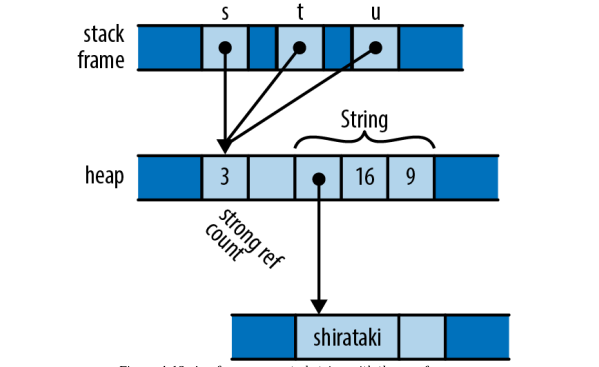
\includegraphics[width=0.8\textwidth]{../img/f4-12.png}
    \caption{一个有三个引用的引用计数字符串}
    \label{f4-12}
\end{figure}

这三个\texttt{Rc<String>}指针都指向内存中的同一块内存,这块内存里存储了一个引用计数和一个\texttt{String}。通常的所有权规也适用于\texttt{Rc}指针,当最后一个\texttt{Rc}指针drop时,Rust会同时drop掉\texttt{String}。

你可以直接对\texttt{Rc<String>}使用任何\texttt{String}的方法:
\begin{minted}{Rust}
    assert!(s.contains("shira"));
    assert_eq!(t.find("taki"), Some(5));
    println!("{} are quite chewy, almost bouncy, but lack flavor", u);
\end{minted}

一个\texttt{Rc}指针拥有的值是不可变的。假设你尝试在字符串的结尾添加文本:
\begin{minted}{Rust}
    s.push_str(" noodles");
\end{minted}

Rust将会报错:
\begin{minted}{text}
    error: cannot borrow data in an `Rc` as mutable
      --> ownership/ownership_rc_mutability.rs:13:5
       |
    13 |     s.push_str(" noodles");
       |     ^ cannot borrow as mutable
       |
\end{minted}

Rust的内存和线程安全保证依赖于没有值既是共享的又是可变的。Rust假设\texttt{Rc}指针指向的值要被共享,因此它必须是不可变的。我们将在\hyperref[ch05]{第5章}解释为什么限制要这么严格。

 使用引用计数来管理内存的一个已知问题就是,如果两个引用计数的值互相指向彼此,那么每一个都会导致对方的引用计数不可能降到0,因此值永远不会被释放(\hyperref[f4-13]{图4-13})。

 \begin{figure}[htbp]
    \centering
    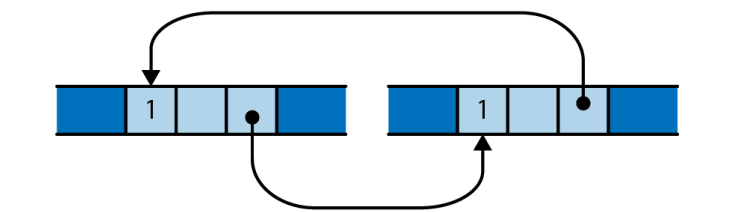
\includegraphics[width=0.8\textwidth]{../img/f4-13.png}
    \caption{一个引用计数循环,这些对象永远不会被释放}
    \label{f4-13}
 \end{figure}

在Rust中出现这种泄漏是可能的,但这种情况非常少见。要想创建这样一个循环,你必须让旧值指向新值,这也意味着旧值要是可变的。因为\texttt{Rc}指针指向的值不可变,所以通常是不能创建这样的循环的。然而,Rust确实提供了一些方法创建部分可变的值的方法;这被称为\emph{内部可变性},我们将在\hyperref[intermut]{内部可变性}一节中介绍。如果你将那些技术和\texttt{Rc}指针结合使用,那么你确实能创建出一个循环,然后造成内存泄漏。

你可以使用\emph{弱指针}\texttt{std::rc::Weak}来避免使用\texttt{Rc}指针创建循环的情况。然而,我们不会在本书中介绍这些,你可以查看标准库的文档获取详情。

move和引用计数指针是两种缓解所有权树过于死板的方法。在下一章中,我们将看到第三种方法:借用值的引用。一旦你对所有权和借用都感到很舒服,那你就已经跨过了Rust的学习曲线中最陡峭的部分,而且已经准备好接受Rust独特的优势。

    \chapter{引用}\label{ch05}

\emph{Libraries cannot provide new inabilities.}

\begin{flushright}
——Mark Miller
\end{flushright}

我们至今为止见过的所有指针类型——简单的\texttt{Box<T>}堆指针、\texttt{String}和\texttt{Vec}内部的指针都拥有值:当所有者被drop时,指针指向的值也会随之消失。Rust还有非拥有指针类型,称为\emph{引用},引用对指向的值的生命周期没有影响。

事实上,正相反,引用绝不应该比它们指向的值活的更长。你必须在你的代码中明确表明,引用的生命寿命比它指向的值更短。为了强调这一点,Rust将创建某个值的引用称为\emph{借用}值:你最终必须把你借走的还给它的所有者。

如果你在读到“你必须在你的代码中明确表明”时感到一丝怀疑,那说明你很优秀。引用自身并没有什么特殊的——本质上,它们只是地址。但保证它们安全的规则是Rust独有的,你以前不可能看到过类似的。尽管这些规则是Rust里最难掌握的部分,但它们能防止的经典的、日常的bug的范围之广令人惊讶,它们对多线程的影响也正在显现。这也是Rust的赌注。

这一章中,我们将讨论Rust中的引用如何工作,展示引用、函数和自定义类型如何包含生命周期信息来保证它们被安全使用,阐释它怎么能在编译期、不引入运行时开销的同时防止常见的bug。

\section{值的引用}

举个例子,假设我们要为文艺复兴时期优秀的艺术家和他们的著名作品建一个表格。Rust的标准库包含一个哈希表类型,所以我们可以像这样定义我们的类型:
\begin{minted}{Rust}
    use std::collections::HashMap;

    type Table = HashMap<String, Vec<String>>;
\end{minted}

换句话说,这是一个把\texttt{String}值映射到\texttt{Vec<String>}值的哈希表,它把艺术家的名字关联到它们的作品的名字。你可以使用\texttt{for}循环来迭代\texttt{HashMap}的条目,因此我们可以写一个函数打印出一个\texttt{Table}:
\begin{minted}{Rust}
    fn show(table: Table) {
        for (artist, works) in table {
            println!("works by {}:", artist);
            for work in works {
                println!("  {}", work);
            }
        }
    }
\end{minted}

构造和打印表格都很直观:
\begin{minted}{Rust}
    fn main() {
        let mut table = Table::new();
        table.insert("Gesualdo".to_string(),
                     vec!["many madrigals".to_string(),
                          "Tenebrae Responsoria".to_string()]);
        table.insert("Caravaggio".to_string(),
                     vec!["The Musicians".to_string(),
                          "The Calling of St. Matthew".to_string()]);
        table.insert("Cellini".to_string(),
                     vec!["Perseus with the head of Medusa".to_string(),
                          "a salt cellar".to_string()]);
        show(table);
    }
\end{minted}

它也能正常工作:
\begin{minted}{text}
    $ cargo run
         Running `/home/jimb/rust/book/fragments/target/debug/fragments`
    works by Gesualdo:
      many madrigals
      Tenebrae Responsoria
    works by Cellini:
      Perseus with the head of Medusa
      a salt cellar
    works by Caravaggio:
      The Musicians
      The Calling of St. Matthew
\end{minted}

但如果你阅读过上一章中有关move的小节,你就会发现\texttt{show}的定义有一些问题。首先,\texttt{HashMap}不是\texttt{Copy}类型——它不可能是,因为它持有动态分配的表格。因此当程序调用\texttt{show(table)}时,整个结构都被移动到函数里,变量\texttt{table}将变为未初始化。(迭代它时没有特定的顺序,你可能会得到一个不同的顺序,不用担心)如果调用者代码尝试继续使用\texttt{table},它会遇到问题:
\begin{minted}{Rust}
    ...
    show(table);
    assert_eq!(table["Gesualdo"][0], "many madrigals");
\end{minted}

Rust会报错\texttt{table}不再可用:
\begin{minted}{text}
    error: borrow of moved value: `table`
       |
    20 |     let mut table = Table::new();
       |         --------- move occurs because `table` has type
       |                   `HashMap<String, Vec<String>>`,
       |                   which does not implement the `Copy` trait
    ...
    31 |     show(table);
       |          ----- value moved here
    32 |     assert_eq!(table["Gesualdo"][0], "many madrigals");
       |                ^^^^^ value borrowed here after move
\end{minted}

事实上,如果我们仔细查看\texttt{show}的定义,会发现外层的\texttt{for}循环获取了哈希表的所有权然后完全消费了它,内层的\texttt{for}循环对每一个vector做了同样的事(我们之前已经在“liberté, égalité, fraternité”的例子中见过这种行为了)。因为move语义,我们仅仅是为了打印它就已经完全销毁了整个结构体。感谢你,Rust!

正确的处理方式是使用引用。引用让你可以访问一个值,同时不影响它的所有权。引用有两种:
\begin{itemize}
    \item \emph{共享引用}让你能读取但不能修改被引用的值。然而,你可以同时持有多个共享引用。表达式\texttt{\&e}返回一个指向\texttt{e}的值的共享引用,如果\texttt{e}的类型是\texttt{T},那么\texttt{\&e}的类型就是\texttt{\&T},读作“ref \texttt{T}”。共享引用是\texttt{Copy}类型。
    \item 如果你有一个值的\emph{可变引用},你可以读取和修改这个值。然而,你不能同时再有任何其他有效的引用。表达式\texttt{\&mut e}返回一个指向\texttt{e}的值的可变引用,它的类型是\texttt{\&mut T},读作“ref mute \texttt{T}”。可变引用不是\texttt{Copy}类型。
\end{itemize}

你可以将共享和可变引用的区别看作是一种在编译期强制\emph{多个读者或一个写者}的规则的方法。事实上,这个规则不仅适用于引用,还适用于被借用的值的所有者。只要一个值有共享引用存在,就算是它的拥有者也不能修改它,这个值被锁定了。当\texttt{show}正在使用\texttt{table}时没有人可以修改\texttt{table}。类似的,当一个值有可变引用时,它会排斥其他所有对这个值的方法,此时你不能使用值的持有者,直到可变引用消失。将共享和可变完全分离开来是内存安全的基础,我们将会在下一章介绍原因。

我们的示例中的打印函数不需要修改表格,只需要读取它的内容。所以调用者可以以共享引用的方式传递表格,像下面这样:
\begin{minted}{Rust}
    show(&table);
\end{minted}

引用是非拥有指针,所以\texttt{table}变量仍然保留着整个数据结构的所有权,\texttt{show}只是借用了它。当然,我们还需要调整\texttt{show}的定义来进行匹配,但你必须仔细看才能看出其中的区别:

\begin{minted}{Rust}
    fn show(table: &Table) {
        for (artist, works) in table {
            println!("works by {}:", artist);
            for work in works {
                println!("  {}", work);
            }
        }
    }
\end{minted}

\texttt{show}的参数\texttt{table}的类型从\texttt{Table}变为了\texttt{\&Table}:不再以值传递表格(会导致所有权移动到函数里),我们现在传递一个共享引用。这就是表面上唯一的变化。但是当我们执行函数体时到底是怎么工作的?

我们原先的版本\texttt{for}循环会获取\texttt{HashMap}的所有权按并消耗它。在我们的新版本中它接受一个\texttt{HashMap}的共享引用,迭代一个\texttt{HashMap}的共享引用被定义为产生每个条目的key和value的引用:\texttt{artist}从一个\texttt{String}变为\texttt{\&string},\texttt{works}从一个\texttt{Vec<String>}变为\texttt{\&Vec<String>}。

内部的循环也有类似的变化。迭代一个vector的共享引用被定义为产生它的每个元素的共享引用,因此\texttt{work}现在是一个\texttt{\&String}。这个函数里不再有任何所有权的变化,而是传递各种无所有权的引用。

现在,如果我们想写一个函数来把每个艺术家的作品按字母顺序排列,一个共享引用显然不够,因为共享引用不允许修改。排序函数需要表格的可变引用:
\begin{minted}{Rust}
    fn sort_works(table: &mut Table) {
        for (_artist, works) in table {
            works.sort();
        }
    }
\end{minted}

然后我们需要传递:
\begin{minted}{Rust}
    sort_works(&mut table);
\end{minted}

这个可变借用授予了\texttt{sort\_works}读取和修改我们的数据结构的能力,以满足vector的\texttt{sort}方法的需要。

当我们以会把所有权移动到函数中的方式传参时,我们称这种方式为\emph{以值}传参。如果我们传递值的引用,我们称之为\emph{以引用}传参。例如,我们通过将以值传参修改为以引用传参修复了\texttt{show}函数。许多语言都有这种区别,但它在Rust中尤其重要,因为它阐明了所有权如何被引用影响。

\section{使用引用}

上面的例子展示了引用的一个经典引用:允许函数在不获取所有权的情况下访问或者操作一个数据结构。但引用要更加灵活,让我们通过一些例子来进行更深入的了解。

\subsection{Rust的引用 vs C++的引用}
如果你熟悉C++的引用,你会发现它和Rust中的引用有很多相似之处。最重要的是,它们在机器层面都只是地址。但在实践中,Rust的引用使用起来有一种不同的感觉。

在C++中,引用通常通过隐式转换来创建,然后隐式解引用:
\begin{minted}{Rust}
    // C++代码!
    int x = 10;
    int &r = x;         // 初始化时隐式创建引用
    assert(r == 10);    // 隐式解引用r来访问x的值
    r = 20;             // 把20存储到x中,r仍然指向x
\end{minted}

在Rust中,引用通过\texttt{\&}运算符显示创建,通过\texttt{\*}运算符显式解引用:
\begin{minted}{Rust}
    // 从现在开始回到Rust的代码。
    let x = 10;
    let r = &x;         // &x是一个x的共享引用
    assert!(*r == 10);  // 显式解引用r
\end{minted}

要想创建可变引用,使用\texttt{\&mut}运算符:
\begin{minted}{Rust}
    let mut y = 32;
    let m = &mut y;     // &mut y是y的一个可变引用
    *m += 32;           // 显式解引用m来访问y的值
    assert!(*m == 64);  // 查看y的新值
\end{minted}

但是你可能回想起来,我们修改\texttt{show}函数让它以引用获取艺术家的表格时,我们从来没有使用过\texttt{*}运算符。这是为什么呢?

因为引用在Rust中使用如此广泛,所以如果需要的话,\texttt{.}运算符会隐式解引用它左侧的操作数:
\begin{minted}{Rust}
    struct Anime { name: &'static str, bechdel_pass: bool };
    let aria = Anime { name: "Aria: The Animation", bechdel_pass: true };
    let anime_ref = &aria;
    assert_eq!(anime_ref.name, "Aria: The Animation");

    // 等价于上面的代码,但显式写出了解引用
    assert_eq!((*anime_ref).name, "Aria: The Animation");
\end{minted}

\texttt{show}函数里使用的\texttt{println!}宏会展开为使用\texttt{.}运算符的代码,因此它也利用了这种隐式解引用。

如果方法调用需要的话,\texttt{.}运算符还会隐式借用左侧操作数的引用。例如,\texttt{Vec}的\texttt{sort}方法会获取vector的可变引用,因此下面的两个调用时等价的:
\begin{minted}{Rust}
    let mut v = vec![1973, 1968];
    v.sort();           // 隐式借用v的可变引用
    (&mut v).sort();    // 等价写法,不过更详细
\end{minted}

简而言之,C++在引用和左值(指向某个内存地址的表达式)之间隐式转换,如果需要这种转换会在任何地方出现;而在Rust中使用\texttt{\&}和\texttt{*}运算符来创建和解引用,除了\texttt{.}运算符是个例外,它会自动隐式借用和解引用。













    \chapter{表达式}\label{ch06}

\emph{LISP programmers know the value of everything, but the cost of nothing}

\begin{flushright}
    ——Alan Perlis, epigram #55
\end{flushright}

在这一章中,我们将介绍Rust的\emph{表达式},它是构成Rust函数体和大部分Rust代码的构建块。Rust中大部分都是表达式。在这一章中,我们将探索表达式的力量以及如何克服它的局限。我们还将介绍控制流,它在Rust中完全是以表达式为基础的,最后还要介绍Rust中的基本运算符如何单独和组合工作。

还有一些从技术角度应该划入这一类的概念,例如闭包和迭代器,因为足够重要因此我们之后会用单独的章节介绍它们。现在,我们希望能用尽可能少的页数介绍尽可能多的语法。

\section{表达式语言}

Rust表面上看上去像C家族的语言,但这其实是一个误解。在C语言中,\emph{表达式}和\emph{语句}之间有很大的不同。表达式是一些像这样的代码:
\begin{minted}{C}
    5 * (fahr-32) / 9
\end{minted}
而语句则是像这样的:
\begin{minted}{C}
    for (; begin != end; ++begin) {
        if (*begin == target)
            break;
    }
\end{minted}
表达式有值,但语句没有。

Rust是一种\emph{表达式语言}。这意味着它遵循了起源于Lisp的传统,也就是表达式负责完成所有工作。

在C中,\texttt{if}和\texttt{switch}是语句。它们并不产生值,也不能被用在表达式中间。在Rust中,\texttt{if}和\texttt{match}\emph{可以}产生值。我们已经在\hyperref[ch02]{第2章}中看到过一个产生数字值的\texttt{match}表达式:
\begin{minted}{Rust}
    pixels[r * bounds.0 + c] =
        match escapes(Complex { re: point.0, im: point.1 }, 255) {
            None => 0,
            Some(count) => 255 - count as u8
        };
\end{minted}

一个\texttt{if}表达式可以用于初始化一个变量:
\begin{minted}{Rust}
    let status =
        if cpu.temperature <= MAX_TEMP {
            HttpStatus::Ok
        } else {
            HttpStatus::ServerError  // server melted
        };
\end{minted}

一个\texttt{match}表达式可以被用作函数参数或宏的参数:
\begin{minted}{Rust}
    println!("Inside the vat, you see {}.",
        match vat.contents {
            Some(brain) => brain.desc(),
            None => "nothing of interest"
        });
\end{minted}

这解释了Rust为什么没有C的三元运算符\texttt{(expr1 ? expr2 : expr3))}。在C中,它是一种类似\texttt{if}语句的表达式。在Rust中这种写法是多余的,因为\texttt{if}表达式可以同时实现这两种功能。

C中的大部分控制流工具都是语句,在Rust中则全是表达式。

\section{优先级和关联性}

\label{cast}

    \chapter{错误处理}\label{ch07}

\emph{I knew if I stayed around long enough, something like this would happen.}

\begin{flushright}
    ——George Bernard Shaw on dying
\end{flushright}

Rust的错误处理不同寻常,无法用很短的一个章节来介绍它。其实它里面并没有什么困难的概念,只有一些可能对你来说可能很新的概念。这一章将覆盖Rust中两种不同的错误处理:panic和\texttt{Result}。

一般的错误使用\texttt{Result}类型来处理,\texttt{Result}通常代表程序之外的东西引起的问题,例如错误的输入、网络中断、权限问题等。这种情况的出现不由我们决定,即使是一个完全没有bug的程序也可能随时遇到它们。这一章中的大部分内容都是在讨论这种错误。我们将首先介绍panic,因为它比较简单。

panic是另一种错误,一种\emph{永远不应该发生}的错误。

\section{panic}

当程序遇到一些由程序自身的bug导致的非常糟糕的事情时它会panic。例如:
\begin{itemize}
    \item 数组访问越界
    \item 整数除以0
    \item 在值为\texttt{Err}的\texttt{Result}上调用\texttt{.expect()}方法
    \item 断言失败
\end{itemize}

(还有一个宏\texttt{panic!()},用于当你的代码自己发现了错误,想要直接触发panic的情况。\texttt{panic!()}接受可选的\texttt{println!()}-风格的参数,用于构建错误信息。)

这些条件的共同之处在于——它们都是程序员的错。一条好的经验法则是:“不要panic”。

但是我们都有犯错误的时候。当这些不该发生的错误发生了的时候,该怎么办?值得注意的是,Rust给了你一个选择:Rust可以展开堆栈或者中止进程。栈展开是默认行为。

\subsection{栈展开}
当海盗们瓜分抢来的战利品时,船长将得到一半的战利品。普通的船员们均分剩下的一半。(海盗们讨厌分数,因此如果均分时不能除尽,结果会向下取整,余数将分给船上的鹦鹉。)
\begin{minted}{Rust}
    fn pirate_share(total: u64, crew_size: usize) -> u64 {
        let half = total / 2;
        half / crew_size as u64
    }
\end{minted}

这段代码也许可以工作几个世纪,直到有一天船长是抢劫之后唯一的幸存者。如果我们传递的\texttt{crew\_size}为0,它将会除以0。在C++中,这将是未定义行为。在Rust中,它会触发panic,panic通常会按照如下方式继续:
\begin{itemize}
    \item 打印一条错误消息到终端:
    \begin{minted}{text}
    thread 'main' panicked at 'attempt to divide by zero',
    pirates.rs:3780
    note: Run with `RUST_BACKTRACE=1` for a backtrace.
    \end{minted}

    如果你设置了\texttt{RUST\_BACKTRACE}环境变量,Rust还会打印出此时的堆栈信息。

    \item 堆栈被展开。这和C++中的异常处理很像。
    
    任何当前函数内的临时值、局部变量、或者参数都会按照与它们创建时相反的顺序被drop掉。

    drop一个值意味着清理它:函数使用过的任何\texttt{String}或\texttt{Vec}都会被释放,任何打开的\texttt{File}都会被关闭,等等。用户自定义的\texttt{drop}方法也会被调用,见“\hyperref[drop]{Drop}”一节。在\texttt{pirate\_share()}的例子中,没有要清理的内容。

    一旦当前的函数调用被清理完毕,我们会移动到它的调用者,以同样的方式drop它的变量和参数。然后我们移动到\emph{那个}函数的调用者,以此类推。

    \item 最后,线程退出。如果panic的线程是主线程,整个进程会退出(退出代码不为0)。
\end{itemize}

对这种有序的处理,也许\emph{panic}是一个有误导性的名字。panic并不是崩溃,也不是未定义行为,它更类似于Java中的\texttt{RuntimeException}或C++中的\texttt{std::logic\_error}。它的行为都是良定义的,它只是不应该发生。

panic是安全的。它不违背Rust中的任何安全规则,即使你设法在一个标准库的方法中引起panic,它也用于不会导致悬垂指针或者初始化到一半的值。关键在于Rust在任何错误的事情发生之前就捕捉到了无效的数组访问或者类似的情况。如果继续下去将是不安全的,所以Rust会展开堆栈。但进程的其他部分可以继续运行。

panic是以线程为单位。一个线程可以panic,而其他线程继续处理它们的业务。在\hyperref[ch19]{第19章}中,我们会展示一个父线程怎么查明一个子线程是否panic并优雅地处理错误。

还有一种方式\emph{捕获}栈展开,允许线程存活并继续运行。标准库函数\texttt{std::panic::catch\_unwind()}可以做到这一点。我们不会解释如何使用它,但Rust的测试工具使用了这个机制,用于在测试时断言失败的情况下恢复执行(当编写可以在C或C++中调用的Rust代码时这也是必须的,因为在非Rust代码中的栈展开是未定义行为,见\hyperref[ch22]{第22章})。

理想情况下,我们希望没有bug并且永远不会panic的代码。但没有完美的事物,你可以使用线程和\texttt{catch\_unwind()}来处理panic,让你的程序更加健壮。一个重要的警告是这些工具只会捕获展开堆栈的panic。不是所有的panic都以这种方式处理。

\subsection{中止}


\section{Result}

\subsection{捕捉错误}

\subsection{Result类型别名}

\subsection{打印错误}

\subsection{传播错误}\label{properror}
    \chapter{crate与模块}\label{ch08}

\emph{This is one note in a Rust theme: systems programmers can have nice things.}

\begin{flushright}
    ——Robert O'Callahan, “\href{https://robert.ocallahan.org/2016/08/random-thoughts-on-rust-cratesio-and.html}{Random Thoughts on Rust: crates.io and IDEs}”
\end{flushright}

假设你在编写一个仿真蕨类植物从细胞开始生长的程序。你的程序就像蕨类一样,一开始非常简单,可能所有代码都在单个文件里——就像一个孢子。随着它逐渐成长,它开始逐渐建立起内部的结构,不同的片段负责不同的功能。它将分裂为多个文件,可能覆盖整个目录树。随着时间的推移,它可能会成为整个软件生态系统的重要组成部分 。对于任何成长到不仅仅是几个数据结构和几百行代码的程序,都必须要对代码进行组织。

这一章将会介绍Rust中用于组织程序的特性:crate和模块。我们还会介绍Rust crate的结构和分发相关的话题,包括如何编写文档和测试Rust代码,如何禁用不需要的编译器警告,如何使用Cargo来管理项目依赖和版本,如何在Rust的公开crate仓库:crates.io上发布开源的库,crate的版本如何演变,等等。我们将使用蕨类仿真程序作为我们的例子。

\section{Crate}

Rust程序由\emph{crates}组成。每一个crate都是一个完整的、一体的单元:一个库或可执行文件的所有代码、加上相关的测试、示例、工具、配置、以及一些其他东西。为了编写你自己的蕨类模拟器,你可能需要使用和3D图形、生物信息学、并行计算等相关的第三方库。这些库就像箱子一样(见\hyperref[f8-1]{图8-1})。

\begin{figure}[htbp]
    \centering
    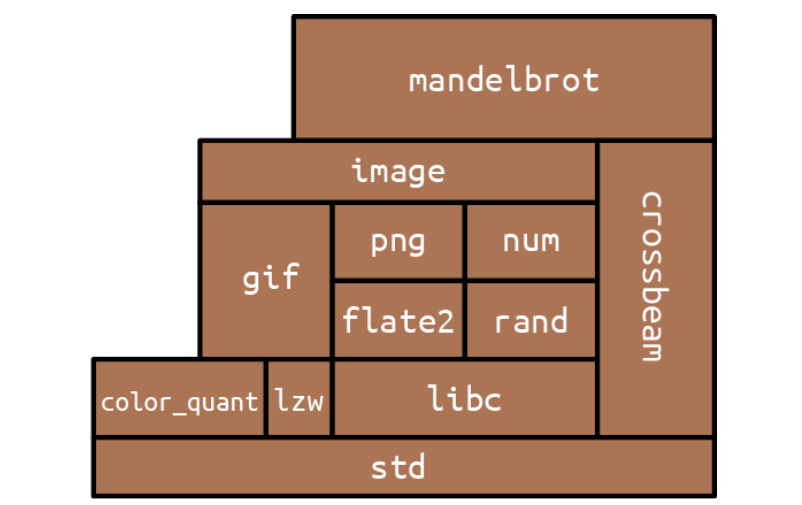
\includegraphics[width=0.9\textwidth]{../img/f8-1.png}
    \caption{一个crate和它的依赖}
    \label{f8-1}
\end{figure}

查看crate是什么以及它们是如何工作的最简单方法就是使用带有\texttt{--verbose}参数的\texttt{cargo build}来构建一个有一些依赖的程序。我们用“\hyperref[mandelbrot]{一个并发的曼德勃罗集}”作为示例。结果如下所示:
\begin{minted}{text}
    $ cd mandelbrot
    $ cargo clean   # delete previously compiled code
    $ cargo build --verbose
        Updating registry `https://github.com/rust-lang/crates.io-index`
     Downloading autocfg v1.0.0
     Downloading semver-parser v0.7.0
     Downloading gif v0.9.0
     Downloading png v0.7.0
    
    ... (downloading and compiling many more crates)

        Compiling jpeg-decoder v0.1.18
          Running `rustc
             --crate-name jpeg_decoder
             --crate-type lib
             ...
             --extern byteorder=.../libbyteorder-29efdd0b59c6f920.rmeta
             ...
        Compiling image v0.13.0
          Running `rustc
             --crate--name image
             --crate-type lib
             ...
             --extern byteorder=.../libbyteorder-29efdd0b59c6f920.rmeta
             --extern gif=.../libgif-a7006d35f1b58972.rmeta
             --extern jpeg_decoder=.../libjped_decoder-5c10558d0d57d300.rmeta
        Compiling mandelbrot v0.1.0 (/tmp/rustbook-test-files/mandelbrot)
          Running `rustc
             --edition=2018
             --crate-name mandelbrot
             --crate-type bin
             ...
             --extern crossbeam=.../libcrossbeam-f87b4b3d3284acc2.rlib
             --extern image=.../libimage-b5737c12bd641c43.rlib
             --extern num=.../libnum-1974e9a1dc582ba7.rlib -C link-arg=-fuse-ld=lld`
         Finished dev [unoptimized + debuginfo] target(s) in 16.94s
\end{minted}

我们重新格式化了\texttt{rustc}的命令行来改善可读性,并且删掉了很多和我们的讨论无关的编译器选项,用省略号(\ldots)代替了它们。

你可能还记得,当我们完成曼德勃罗集程序时,它的\texttt{main.rs}包含几个引入其它crate的\texttt{use}声明:
\begin{minted}{Rust}
    use num::Complex;
    // ...
    use image::ColorType;
    use image::png::PNGEncoder;
\end{minted}

哦我们还在\texttt{Cargo.toml}中指定了每个crate的版本:
\begin{minted}{toml}
    [dependencies]
    num = "0.4"
    image = "0.13"
    crossbeam = "0.8"
\end{minted}

这里的\emph{依赖}指这个程序使用的其它crate,也就是我们依赖的代码。我们可以在\href{https://crates.io}{crates.io}中找到这些crate,那是Rust社区用于存放开源的crate的网站。例如,我们可以访问crates.io并搜索图片库来找到\texttt{image}库。crates.io上的每个crate的页面上会显示它的\texttt{README.md}文件和到文档和源代码的链接,还有一行配置例如\texttt{image = "0.13"},你可以复制这一行并添加到你的\texttt{Crago.toml}中。这里显示的版本号直接用了我们在编写这个程序时这三个包的最新版本。

Cargo的输出说明了这些信息是如何被使用的。当我们运行\texttt{cargo build}时,Cargo会首先从crates.io下载这些crate的指定版本的源码。然后,它读取那些crate的\texttt{Cargo.toml}文件,下载\emph{它们}的依赖,然后递归操作。例如,\texttt{image} crate的0.13.0版本的源代码中包含一个\texttt{Cargo.toml}文件,内容如下:
\begin{minted}{toml}
    [dependencies]
    byteorder = "1.0.0"
    num-iter = "0.1.32"
    num-rational = "0.1.32"
    num-traits = "0.1.32"
    enum_primitive = "0.1.0"
\end{minted}

看到这些内容,Cargo知道在它可以使用\texttt{image}之前,它必须先拉取这些crate。我们称它们为\texttt{mandelbrot}的\emph{间接(transitive)}依赖。所有这些依赖的集合告诉了Cargo需要知道的有关如何构建和构建顺序的一切信息,它被称为crate的\emph{依赖图}。Cargo自动处理依赖图和间接依赖的能力是程序员们付出时间和努力的一大胜利。

当获得了源代码之后,Cargo会编译所有的crate。它会运行Rust的编译器\texttt{rustc},一次编译依赖图中的一个crate。当编译这些库时,Cargo会使用\texttt{--crate-type lib}选项。这告诉\texttt{rustc}不要寻找\texttt{main()}函数,而是产生一个包含编译过代码的\texttt{.rlib}文件,这个文件可以被用于创建可执行文件和其他\texttt{.rlib}文件。

当编译程序时,Cargo会使用\texttt{--crate-type bin},编译的结果将是一个目标平台的二进制可执行文件:例如在Windows上就是\texttt{mandelbrot.exe}。

对于每一个\texttt{rustc}命令,Cargo都会传递\texttt{--extern}选项,给出crate用到的每一个库的名称。这样,当\texttt{rustc}看到一行类似于\texttt{use image::png::PNGEncoder}的代码时,它可以分辨出\texttt{image}是另一个crate的名字,而且Cargo传递的选项让它知道该从哪里寻找编译好的crate。Rust的编译器需要访问这些\texttt{.rlib}文件,因为它们包含编译好的库中的代码。Rust将会将代码静态链接到最终的可执行文件中。\texttt{.rlib}还包含类型信息,因此Rust可以通过检查确保我们在代码中使用的库的特性确实存在而且被正确使用。它还包含一份crate的public内联函数、泛型、宏、特性的拷贝,这些东西只有当Rust看到我们如何使用它们时才可以将它们编译为机器代码。

\texttt{cargo build}支持各种选项,其中的大部分都超出了本书的范围,不过我们在这里会提到其中一个:\texttt{cargo build --release}会生成优化后的构建。Release构建运行得更快,但需要更长的时间来编译,而且它们不检查整数溢出、跳过\texttt{debug\_assert!()}断言,并且它们在panic生成的堆栈追踪通常不太可靠。

\subsection{版本}

Rust有极强的兼容性保证。任何在Rust 1.0中能编译的代码必须在Rust 1.50或者1.900(如果发布了的话)中也能编译。


但有时社区会遇到一些令人信服的扩展语言的建议,这可能会导致旧代码不能再编译。例如,经过了多次讨论之后,Rust确定了一种支持异步编程的语法,将标识符\texttt{async}和\texttt{await}重新用作关键字(见\hyperref[ch20]{第20章})。但这项语言的改变可能会导致使用\texttt{async}或者\texttt{await}作为变量名的代码不能再编译。

为了在不破坏这些现有代码的前提下演变,Rust使用了\emph{版本}。Rust的2015版本和Rust 1.0兼容。2018版本将\texttt{async}和\texttt{await}改为关键字、精简了模块系统、还引入了一些和2015版本不兼容的其它语言更改。每个crate在\texttt{Cargo.toml}文件中的\texttt{package}节中用一行类似如下的说明指定Rust的版本:
\begin{minted}{Rust}
    edition = "2018"
\end{minted}

如果缺少这个关键字,将会假设使用2015版本,因此旧的crate完全不需要做任何更改。但如果你想使用异步函数或者新的模块系统,你需要确保\texttt{Cargo.toml}中有\texttt{edition = "2018"}(或者可能更新的版本)。

Rust保证编译器将总是接受语言的所有版本,并且程序可以自由混合使用不同版本编写的crate。即使一个2015版本的crate依赖一个2018版本的crate也没有问题。换句话说,一个crate的版本只影响它的代码是如何被构建的,版本的区别只体现在代码编译的时候。这意味着没有必要更新旧的版本来适配现代Rust的生态。类似的,也没有必要将crate保持在旧版本来避免影响到它的用户。你只需要在想使用新的语言特性时更改自己代码中的版本。

版本并不是每年都会更新,只有当Rust项目觉得有必要出新版本的时候才会更新。例如,没有2020版本。把\texttt{edition}设置为\texttt{"2020"}将会导致错误。\href{https://doc.rust-lang.org/stable/edition-guide}{Rust版本指南}介绍了每一个版本中的变化,并提供了版本系统的背景知识。

使用最新版本几乎总是一个好主意,尤其是新编写代码时。\texttt{cargo new}会默认创建最新版本的项目。这本书中将始终使用2018版本。

如果你有一个用更旧版本的Rust编写的crate,\texttt{cargo fix}命令也许可以帮你自动把代码更新到更新的版本。Rust版本指南详细解释了\texttt{cargo fix}命令。

\subsection{构建配置}
有几个\texttt{Cargo.toml}中的配置选项可以影响到\texttt{cargo}生成的\texttt{rustc}命令行(\hyperref[t8-1]{表8-1})。

\begin{table}[htbp]
    \caption{Cargo.toml配置节}
    \centering
    \begin{tabular}{ll}
        \hline
        \textbf{命令行}     & \texttt{使用到的Cargo.toml节}   \\
        \hline
        \texttt{cargo build} & \texttt{[profile.dev]}   \\
        \rowcolor{tablecolor}
        \texttt{cargo build --release} & \texttt{[profile.release]} \\
        \texttt{cargo test}  & \texttt{[profile.test]}  \\
    \end{tabular}
\end{table}

通常默认的行为就足够了,但我们会发现一个例外是你想使用一个profiler——一个用于测量程序使用CPU时间情况的工具。为了从profiler获取最准确的数据,你将同时需要优化(通常只在release构建中可用)和调试符号(通常只在debug构建中可用)。为了同时启用两者,在\texttt{Cargo.toml}中添加:
\begin{minted}{toml}
    [profile.release]
    debug = true    # 允许在release构建中启用调试符号
\end{minted}

\texttt{debug}设置控制是否给\texttt{rustc}传递\texttt{-g}选项。有了这个配置,当你输入\texttt{cargo build --release}时,你将会得到一个带有调试符号的二进制文件。优化的设置将不会被影响。

\hyperref[https://doc.rust-lang.org/cargo/reference/manifest.html]{Cargo文档}中列出了很多其他你可以在\texttt{Cargo.toml}中调整的设置。

\section{模块}

如果说crate决定了项目之间的代码共享,那么\emph{模块}则决定了项目\emph{内部}的代码组织。它们扮演了Rust中的命名空间——一种包含函数、类型、常量等内容的容器,这些模块组成了你的Rust程序或库。一个模块看起来类似于这样:

\begin{minted}{Rust}
    mod spores {
        use cells::{Cell, Gene};

        /// 成熟蕨类植物产生的细胞。它会随着风飘散,
        /// 这也是蕨类生命周期的一部分。一个孢子会成长为一个原叶体——
        /// 一个宽达5mm的完整的独立有机体。它会产生受精卵,
        /// 这些受精卵会成长为新的蕨类植物(植物的性别很复杂)。
        pub struct Spore {
            ...
        }

        /// 模拟通过减数分裂产生孢子的过程。
        pub fn produce_spore(factory: &mut Sporangium) -> Spore {
            ...
        }

        // 提取一个孢子中的基因。
        pub(crate) fn genes(spore: &Spore) -> Vec<Gene> {
            ...
        }

        /// 混合基因为减数分裂做准备(分裂间期的一部分)。
        fn recombine(parent: &mut Cell) {
            ...
        }

        ...
    }
\end{minted}

一个模块是\emph{item}的集合,\texttt{item}是命名的特性例如例子中的\texttt{Spore}结构体和两个函数。\texttt{pub}关键字将item设为公有的,因此可以从模块外边访问。

一个函数被标记为\texttt{pub(crate)},意味着它在这个crate中任何地方都可以访问,但不作为外部接口的一部分公开。它不能被其他crate使用,也不会在crate的文档中显示。

任何没有被标记为\texttt{pub}的都是私有的,只能在定义它的模块和子模块中使用:
\begin{minted}{Rust}
    let s = spores::produce_spore(&mut factory);    // ok
    
    spores::recombine(&mut cell);   // 错误:`recombine`是私有的
\end{minted}

将item标记为\emph{pub}通常称为“导出”这个item。

这一节的剩余部分将覆盖使用模块所需要了解的细节:
\begin{itemize}
    \item 我们会展示如果需要的话怎么嵌套模块和把它们分布在不同的文件和目录中。
    \item 我们会解释Rust从其他模块中引用item的路径语法,并展示怎么导入item,这样就不需要每次都写出完整的路径。
    \item 我们会接触Rust对结构体字段的细粒度控制。
    \item 我们会介绍\emph{prelude}模块,它通过收集几乎所有用户都会用到的常见导入来减少重复的导入。
    \item 我们会展示\emph{常量}和\emph{静态量},这是两种为了清晰和一致性而设计的定义命名变量的方式。
\end{itemize}

\subsection{嵌套模块}

模块可以嵌套,事实上一个模块只是一些子模块的集合的情况是很常见的:
\begin{minted}{Rust}
    mod plant_structures {
        pub mod roots {
            ...
        }
        pub mod stems {
            ...
        }
        pub mod leaves {
            ...
        }
    }
\end{minted}

如果你想要让嵌套模块中的一个item对其他crate可见,那需要保证将它\emph{和所有嵌套包含它的模块}标记为public。否则你会看到一个类似这样的警告:
\begin{minted}{text}
    warning: function is never used: `is_square`
      --> src/crates_unused_items.rs:23:9
       |
    23 | /         pub fn is_square(root: &Root) -> bool {
    24 | |             root.cross_section_shape().is_square()
    25 | |         }
       | |_________^
       |
\end{minted}

可能这个函数这时确实是死代码。但如果你是想将它用在其他crate中,Rust会让你明白它实际上并不可见。你需要保证嵌套包含它的模块也都被标记为\texttt{pub}。

也可以声明\texttt{pub(super)},让一个item只在父模块中可见。\texttt{pub(in <path>)}可以让它在一个指定的父模块和其后代中可见。这在深层嵌套的模块中很有用:
\begin{minted}{Rust}
    mod plant_structures {
        pub mod roots {
            pub mod products {
                pub(in crate::plant_structures::roots) struct Cytokinin {
                    ...
                }
            }

            use products::Cytokinin;    // ok: 在`roots`模块中
        }

        use roots::products::Cytokinin; // error: `Cytokinin`是私有的
    }

    // error: `Cytokinin`是私有的
    use plant_structures::roots::products::Cytokinin;
\end{minted}

通过这种方式,我们可以写出一个有数量庞大的代码和完整的模块层次结构的程序,不管这些模块的关系如何,我们都可以将整个程序写在单个文件里。

但实际上以这种方式来工作非常的痛苦,因此还有另一种方案。

\subsection{单独文件中的模块}
一个模块还可以这么写:
\begin{minted}{Rust}
    mod spores;
\end{minted}

之前,我们还在花括号中包含了\texttt{spores}模块的主体。这里,我们通过这种方式告诉Rust编译器\texttt{spores}模块在一个单独的叫\texttt{spores.rs}的文件里:
\begin{minted}{Rust}
    // spores.rs

    /// 成熟蕨类植物产生的一个细胞...
    pub struct Spore {
        ...
    }

    /// 模拟减数分裂产生孢子的过程。
    pub fn produce_spore(factory: &mut Sporangium) -> Spore {
        ...
    }

    /// 从一个孢子中提取基因。
    pub(crate) fn genes(spore: &Spore) -> Vec<Gene> {
        ...
    }

    /// 混合基因为减数分裂做准备(分裂间期的一部分)。
    fn recombine(parent: &mut Cell) {
        ...
    }
\end{minted}

\texttt{spores.rs}只包含组成模块的item。它并不需要任何说明来表明它是一个模块。

这个\texttt{spores}模块和我们在上一节中展示的版本的\emph{唯一}不同就是代码的位置。有关公有性和私有性的规则和之前完全相同。Rust从来不会单独编译模块,即使它们在单独的文件里。当你构建一个Rust的crate的时候,你总是要重新编译它里面所有的模块。

一个模块也可以有自己的目录。当Rust看到\texttt{mod spores;}时,它会检查\texttt{spores.rs}和\texttt{spores/mod.rs},如果这两个文件都不存在或者都存在就会报错。这个例子中我们使用了\texttt{spores.rs},因为\texttt{spores}模块没有任何子模块。但考虑一下我们之前写的\texttt{plant\_structures}模块。如果我们决定将那个模块和它的三个字模块分割在单独的文件中,最终的项目看起来就是这样:
\begin{minted}{text}
    fern_sim/
    |—— Cargo.toml
    |—— src/
        |—— main.rs
        |—— spores.rs
        |—— plant_structures/
            |—— mod.rs
            |—— leaves.rs
            |—— roots.rs
            |—— stems.rs
\end{minted}

在\texttt{main.rs}中,我们声明了\texttt{plant\_structures}模块:
\begin{minted}{Rust}
    pub mod plant_structures;
\end{minted}

这会导致Rust去加载\texttt{plant\_structures/mod.rs},这个文件里又声明了三个子模块:
\begin{minted}{Rust}
    // 在plant_structures/mod.rs中
    pub mod roots;
    pub mod stems;
    pub mod leaves;
\end{minted}

这三个模块的内容都被存储在单独的文件中,分别命名为\texttt{leaves.rs}、\texttt{roots.rs}、\texttt{stems.rs},和\texttt{mod.rs}一样在\texttt{plant\_structures}目录下。

使用同名的文件和目录来组成模块也是有可能的。例如,如果\texttt{stems}需要包含两个分别叫\texttt{xylem}和\texttt{phloem}的模块,我们可以选择将\texttt{stems}保留在\texttt{plant\_structures/stems.rs}中,然后添加一个新的\texttt{stems}目录:
\begin{minted}{Rust}
    fern_sim/
    |—— Cargo.toml
    |—— src/
        |—— main.rs
        |—— spores.rs
        |—— plant_structures/
            |—— mod.rs
            |—— leaves.rs
            |—— roots.rs
            |—— stems/
            |   |—— phloem.rs
            |   |—— xylem.rs
            |—— stems.rs
\end{minted}

然后在\texttt{stems.rs}中声明这两个新的子模块:
\begin{minted}{Rust}
    // 在plant_structures/stems.rs中
    pub mod xylem;
    pub mod phloem;
\end{minted}

这三种方式——模块在自己单独的文件中、模块在自己同名的目录中的\texttt{mod.rs}中,模块在自己单独的文件中并有一个同名的目录包含子模块——给了模块系统足够的灵活性来支撑你需要的任何程序结构。

\subsection{路径和导入}
\texttt{::}运算符用于访问模块中的特性。你的项目中任何地方的代码都可以通过路径来引用任何标准库的特性:
\begin{minted}{Rust}
    if s1 > s2 {
        std::mem::swap(&mut s1, &mut s2);
    }
\end{minted}

\texttt{std}是标准库的名称。路径\texttt{std}指向标准库的顶级模块。\texttt{std::mem}是在标准库中的一个子模块,\texttt{std::mem::swap}是\texttt{std::mem}模块中的一个public函数。

你可以始终用这方式编写所有的代码,每当你需要圆或字典时都写出\texttt{std::f64::consts::PI}和\texttt{std::collections::HashMap::new},但这样太过繁琐,而且难以阅读。替代方案是把一些特性\emph{导入}用到它们的模块:
\begin{minted}{Rust}
    use std::mem;

    if s1 > s2 {
        mem::swap(&mut s1, &mut s2);
    }
\end{minted}

\texttt{use}声明会导致\texttt{mem}变为\texttt{std::mem}在整个块或模块中的一个局部别名。

你也可以编写\texttt{std::mem::swap}来导入\texttt{swap}函数本身,而不是\texttt{mem}模块。然而,我们之前的方式被认为是最佳的风格:引入类型、trait和模块(例如\texttt{std::mem})然后使用相对路径访问函数、常量和其他成员。

可以依次导入若干个名字:
\begin{minted}{Rust}
    use std::collections::{HashMap, HashSet};   // 导入两个
    
    use std::fs::{self, File};  // 导入`std::fs`和`std::fs::File`
    
    use std::io::prelude::*;    // 导入所有内容
\end{minted}

这是写出所有单独导入的方式的缩写:
\begin{minted}{Rust}
    use std::collections::HashMap;
    use std::collections::HashSet;

    use std::fs;
    use std::fs::File;

    // std::io::prelude中的所有public item:
    use std::io::prelude::Read;
    use std::io::prelude::Write;
    use std::io::prelude::BufRead;
    use std::io::prelude::Seek;
\end{minted}

你可以使用\texttt{as}导入一个item并同时给它一个不同的局部名称:
\begin{minted}{Rust}
    use std::io::Result as IOResult;

    // 返回类型等价于`std::io::Result<()>`
    fn save_spore(spore: &Spore) -> IOResult<()>
    ...
\end{minted}

模块并不会\emph{自动}从父模块中继承名称。例如,假设我们的\texttt{proteins/mod.rs}有如下内容:
\begin{minted}{Rust}
    // proteins/mod.rs
    pub enum AminoAcid { ... }
    pub mod synthesis;
\end{minted}

那么\texttt{synthesis.rs}里的代码并不会自动导入类型\texttt{AminoAcid}:
\begin{minted}{Rust}
    // proteins/synthesis.rs
    pub fn synthesis(seq: &[AminoAcid]) // 错误:找不到类型`AminoAcid`
        ...
\end{minted}

每一个模块都会以空白的状态开始,必须导入它使用的名称:
\begin{minted}{Rust}
    // proteins/synthesis.rs
    use super::AminoAcid;   // 显式地从父模块中导入
    pub fn synthesize(seq: &[AminoAcid]) // ok
        ...
\end{minted}

默认情况下,路径是相对于当前模块的:
\begin{minted}{Rust}
    // 在proteins/mod.rs中

    // 从子模块中导入
    use synthesis::synthesize;
\end{minted}

\texttt{self}也是当前模块的同义词,因此我们可以写:
\begin{minted}{Rust}
    // 在proteins/mod.rs中

    // 导入一个枚举中的名字
    // 这样我们可以用`Lys`来表示赖氨酸,而不是`AminoAcid::Lys`
    use self::AminoAcid::*;
\end{minted}

或者简写为:
\begin{minted}{Rust}
    // 在proteins/mod.rs中

    use AminoAcid::*;
\end{minted}

(这里的\texttt{AminoAcid}的例子,有些违背我们之前提到的只导入类型、trait和模块的风格。如果我们的程序包含很长的氨基酸序列,那么根据奥威尔的第六原则:“Break any of these rules sooner than say anything outright barbarous.”(绝不要用粗俗语言,为此可以打破上面任一规则。)这么做也是有道理的。

路径中的\texttt{super}和\texttt{crate}关键字有特殊的含义:\texttt{super}指代父模块,\texttt{crate}指代包含当前模块的crate。

使用相对于crate根的路径而不是相对于当前模块的路径可以使在项目中移动代码变得更容易,因为这样的话计算当前模块的路径变了,导入也不会出错。例如,我们可以使用\texttt{crate}来写\texttt{synthesis.rs}:
\begin{minted}{Rust}
    // proteins/synthesis.rs
    use crate::proteins::AminoAcid; // 显式的相对于crate根的导入

    pub fn synthesize(seq: &[AminoAcid]) // ok
        ...
\end{minted}

子模块可以通过\texttt{use super::*}访问父模块中的私有item。

如果你有一个模块和当前正在使用的某一个模块同名,那么引用它们的时候就要小心了。例如,如果你的程序在\texttt{Cargo.toml}列出了\texttt{image} crate依赖,同时还有一个模块叫\texttt{image},那么以\texttt{image}开头的路径将会导致歧义:
\begin{minted}{Rust}
    mod image {
        pub struct Sampler {
            ...
        }
    }

    // 错误:这是指向`imaeg`模块,还是`image` crate?
    use image::Pixels;
\end{minted}

即使\texttt{image}模块没有\texttt{Pixels}类型,这个歧义也会被认为是错误:如果之后又添加了\texttt{Pixels}的定义,那么可能会改变路径指向的内容,这可能会令人迷惑。

为了解决歧义,Rust有一种特殊的路径称为\emph{绝对路径},它们以\texttt{::}开头,将总是指向一个外部的crate。为了指向\texttt{image} crate中的\texttt{Pixels}类型,你可以写:
\begin{minted}{Rust}
    use ::image::Pixels;    // `image` crate的`Pixels`
\end{minted}

为了指向你自己的模块中的`Sampler`类型,你可以写:
\begin{minted}{Rust}
    use self::image::Sampler;   // `image`模块的`Sampler`
\end{minted}

模块和文件的概念并不相同,但模块和Unix文件系统中的文件和目录存在自然的类比关系。\texttt{use}关键字创建别名,就像\texttt{ln}命令创建链接。路径类似于文件名,有绝对路径和相对路径两种形式。\texttt{self}和\texttt{super}类似于\texttt{.}和\texttt{..}这两个特殊的目录。

\subsection{标准prelude}
我们之前说每个模块都以“空白的状态”开始,但事实上并不是\emph{完全}空白的状态。

其中一点是,标准库\texttt{std}被自动链接到每个项目。这意味着你总是可以使用\texttt{std::whatever}这种方式来引用\texttt{std}里的item,例如\texttt{std::mem::swap()}。还有,一些特殊的常见名称,例如\texttt{Vec}和\texttt{Result}也被包含在\emph{标准prelude}中并且被自动导入。具体的行为就好像是包括跟模块在内的每个模块都以如下导入开始:
\begin{minted}{Rust}
    use std::prelude::v1::*;
\end{minted}

标注的prelude包含一些通用的trait和类型。

在\hyperref[ch02]{第2章}中时,我们提到了库有时会提供叫\texttt{prelude}的模块。但\texttt{std::prelude::v1}是唯一一个自动导入的。将一个模块命名为\texttt{prelude}只会一个约定,告诉用户他应该导入\texttt{*}。

\subsection{pub use声明}
即使\texttt{use}声明只是别名,它们也可以是公有的:
\begin{minted}{Rust}
    // in plant_structures/mod.rs
    ...
    pub use self::leaves::Leaf;
    pub use self::roots::Root;
\end{minted}

这意味着\texttt{Leaf}和\texttt{Root}是\texttt{plant\_structures}模块里的public item。它们实际上只是\texttt{plant\_structures::leaves::Leaf}和\texttt{plant\_structures::roots::Root}的别名。

标准的prelude就是以一系列\texttt{pub}导入的方式实现的。

\subsection{pub结构体字段}
一个模块可以包含用户用\texttt{struct}关键字定义的自定义结构体类型。我们将在\hyperref[ch09]{第9章}中介绍细节,但这是一个了解模块如何和结构体字段的可见性交互的好时机。

一个简单的结构体类似这样:
\begin{minted}{Rust}
    pub struct Fern {
        pub roots: RootSet,
        pub stems: StemSet
    }
\end{minted}

一个结构体的所有字段,包括私有字段,都可以在定义结构体的整个模块及其子模块中访问,在模块之外,只有公有的字段才可以被访问。

事实证明通过模块来实现访问控制,而不是像Java和C++那样通过类来实现,对于程序设计将是很大的帮助。不仅能减少重复“getter”和“setter”方法,还能消除类似C++中\texttt{friend}声明的需求。一个模块可以定义几个紧密结合的类型,例如\texttt{frond::LeafMap}和\texttt{frond::LeafMapIter},让它们能按需互相访问彼此的私有字段,同时对程序中的其他部分隐藏实现的细节。

\subsection{静态量和常量}

除了函数、类型和嵌套模块之外,模块里还可以定义\emph{常量}和\emph{静态量}。

\texttt{const}关键字定义常量,语法类似于\texttt{let},除了它必须被标记为\texttt{pub}以及要显式写出类型。还有,为了方便,常量一般都用\texttt{UPPERCASE\_NAMES}:
\begin{minted}{Rust}
    pub const ROOM_TEMPERATURE: f64 = 20.0;     // 摄氏度
\end{minted}

\texttt{static}关键字定义静态量,和\texttt{const}的用法几乎一样:
\begin{minted}{Rust}
    pub static ROOM_TEMPERATURE: f64 = 68.0;    // 华氏温度
\end{minted}

常量有些类似于C++中的\texttt{\#define},值被编译进代码中每一个使用它的地方。一个静态量就是一个在程序开始之前就初始化并持续到程序退出的变量。在代码中使用常量表示幻数和字符串。使用静态量表示更大规模的数据,或者用于需要借用全局常量的引用时。

没有\texttt{mut}常量。静态量可以被标记为\texttt{mut},但就像我们在\hyperref[ch05]{第5章}中讨论的一样,Rust没有任何方法强制实现\texttt{mut}静态量的独占访问。因此,这种变量天生的线程不安全,safe代码完全不能使用它们:
\begin{minted}{Rust}
    static mut PACKETS_SERVED: usize = 0;

    println!("{} served", PACKETS_SERVED);  // 错误:使用了可变的静态量
\end{minted}

Rust不鼓励全局可变的状态。关于替代方案的讨论,见“\nameref{globalvar}”一节。

\section{将程序变为库}

当你的蕨类模拟器完成之后,你决定你需要不止一个程序。假设你还有一个命令行程序运行这个模拟器并把结果保存到文件中。现在,你想要编写其他程序来对保存的结果进行科学分析、实时渲染成长中的植物、渲染逼真的植物等等。所有这些程序都要共享基本的蕨类模拟器的代码。你需要创建一个库。

第一步是将你现有的项目分解为两部分:一个库crate和一个可执行文件。前者包含所有的共享代码,后者包含只有命令行程序才需要的代码。

为了展示怎么做到这一点,让我们给出一个简单粗暴的示例程序:
\begin{minted}{Rust}
    struct Fern {
        size: f64,
        growth_rate: f64
    }

    impl Fern {
        /// 模拟一个蕨类植物一天地成长
        fn grow(&mut self) {
            self.size *= 1.0 + self.growth_rate;
        }
    }

    /// 运行蕨类模拟器模拟几天的变化
    fn run_simulation(fern: &mut Fern, days: usize) {
        for _ in 0 .. days {
            fern.grow();
        }
    }

    fn main() {
        let mut fern = Fern {
            size: 1.0,
            growth_rate: 0.001
        };
        run_simulation(&mut fern, 1000);
        println!("final fern size: {}", fern.size);
    }
\end{minted}

我们假设这个程序有一个普通的\texttt{Cargo.toml}文件:
\begin{minted}{toml}
    [package]
    name = "fern_sim"
    version = "0.1.0"
    authors = ["You <you@example.com>"]
    edition = "2018"
\end{minted}

将这个程序变为库是很简单的。只需要如下步骤:
\begin{enumerate}
    \item 将文件\texttt{src/main.rs}重命名为\texttt{src/lib.rs}
    \item 给\texttt{src/lib.rs}里将作为库的公开特性的item添加\texttt{pub}关键字
    \item 暂时把\texttt{main}函数移动到一个别的临时文件中。我们将很快回来处理它。
\end{enumerate}

最后的\texttt{src/lib.rs}文件看起来像这样:
\begin{minted}{Rust}
    pub struct Fern {
        pub size: f64,
        pub growth_rate: f64
    }

    impl Fern {
        /// 模拟一个蕨类植物一天地成长
        pub fn grow(&mut self) {
            self.size *= 1.0 + self.growth_rate;
        }
    }

    /// 运行蕨类模拟器模拟几天的变化
    pub fn run_simulation(fern: &mut Fern, days: usize) {
        for _ in 0 .. days {
            fern.grow();
        }
    }
\end{minted}

注意我们不需要更改\texttt{Cargo.toml}中的任何内容。这是因为我们最简的\texttt{Cargo.toml}会保持Cargo的默认行为。默认情况下,\texttt{cargo build}会查看源代码目录下的文件然后判断要构建什么。当它看到\texttt{src/lib.rs}文件,它就知道要构建一个库。

\texttt{src/lib.rs}里的代码组成了库的\emph{根模块}。其他使用我们库的crate可以访问跟模块里的公有item。

\section{src/bin目录}









    \chapter{结构体}\label{ch09}

\emph{Long ago, when shepherds wanted to see if two herds of sheep were isomorphic, they would look for an explicit isomorphism}

\begin{flushright}
    ——John C. Baez and James Dolan, “\href{https://arxiv.org/abs/math/9802029}{Categorification}”
\end{flushright}

Rust的结构体,有时也称为\emph{structure},类似于C和C++中的\texttt{struct}类型、Python中的\texttt{class}、JavaScript中的对象。一个结构体把多个不同类型的值组合成单个值,所以你可以将它们作为一个整体进行处理,你也可以读取并且修改结构体的各个组成部分。一个结构体也可以有一些关联的方法来操作它的组成部分。

Rust有三种类型的结构体:\emph{命名字段(name-field)}、\emph{类元组(tuple-like)}、\emph{类单元(unit-like)},它们的区别在于如何引用它们的组成部分:一个命名字段结构体给每一个组件取了一个名字,而类元组结构体用它们出现的顺序来标识它们。类单元结构体没有任何组成部分,它并不常见,但可能比你想象中的更加有用。

在本章中我们将详细解释每一种结构体,并展示它们在内存中的布局。我们将介绍如何给它们添加方法、如何定义可以处理很多不同类型组件的泛型结构体、以及如何让Rust为你的结构体生成通用的trait的实现。

\section{命名字段结构体}

一个命名字段结构体的定义类似于这样:
\begin{minted}{Rust}
    /// 一个8位灰度像素的矩形
    struct GrayscaleMap {
        pixels: Vec<u8>,
        size: (usize, usize)
    }
\end{minted}

这里声明了一个结构体类型\texttt{GrayscaleMap},它有两个字段分别命名为\texttt{pixels}和\texttt{size}。Rust的一个习惯是所有的类型包括结构体,名称中的每一个单词的首字母大写,例如\texttt{GrayscaleMap},这种习惯称为\emph{大驼峰命名法}(或\emph{帕斯卡命名法})。字段和方法名都是小写,用下划线分隔每个单词。这被称为\emph{蛇形命名法}。

你可以用\emph{结构体表达式}构造一个这种类型的值,例如:
\begin{minted}{Rust}
    let width = 1024;
    let height = 576;
    let image = GrayscaleMap {
        pixels: vec![0; width * height],
        size: (width, height)
    };
\end{minted}

结构体表达式以类型名称开始(\texttt{GrayscaleMap}),然后在花括号中列出每一个字段的名称和值。还有一种缩写可以用同名的局部变量来充当字段:
\begin{minted}{Rust}
    fn new_map(size: (usize, usize), pixels: Vec<u8>) -> GrayscaleMap {
        assert_eq!(pixels.len(), size.0 * size.1);
        GrayscaleMap { pixels, size }
    }
\end{minted}

结构体表达式\texttt{GrayscaleMap \{ pixels, size \}}是\texttt{GrayscaleMap \{ pixels: pixels, size: size \}}的缩写。你也可以在使用同名字段缩写的同时使用\texttt{key: value}语法为其它字段赋值。

访问一个结构体的字段需要使用熟悉的\texttt{.}运算符:
\begin{minted}{Rust}
    assert_eq!(image.size, (1024, 476));
    assert_eq!(image.pixels.len(), 1024 * 576);
\end{minted}

和其他item一样,结构体默认是私有的,只在它们声明的模块及其子模块中可见。你可以通过在定义前加\texttt{pub}来让结构体在模块之外也可见。它的每一个字段也是这样,默认也是私有的:
\begin{minted}{Rust}
    /// 一个8位灰度像素的矩形
    pub struct GrayscaleMap {
        pub pixels: Vec<u8>,
        pub size: (usize, usize)
    }
\end{minted}

即使结构体被声明为\texttt{pub},它的字段也可以是私有的:
\begin{minted}{Rust}
    /// 一个8位灰度像素的矩形
    pub struct GrayscaleMap {
        pixels: Vec<u8>,
        size: (usize, usize)
    }
\end{minted}

其他的模块可以使用这个结构体和它的所有公有的关联函数,但不能通过字段名访问私有的字段,也不能通过结构体表达式创建新的\texttt{GrayscaleMap}值。也就是说,创建一个结构体的值要求所有的结构体字段都可见。这也是为什么你不能通过结构体表达式创建新的\texttt{String}或者\texttt{Vec}。这些标准类型都是结构体,但它们的字段全都是私有的。要想创建一个这些类型的值,你必须使用公有的类型关联函数,例如\texttt{Vec::new()}。

在创建一个命名字段结构体值的时候,你可以使用另一个相同类型的结构体来提供你省略的字段的值。在一个结构体表达式中,如果命名字段最后跟着一个\texttt{.. EXPR},那么没有提到的字段将从\texttt{EXPR}中获取值,\texttt{EXPR}必须是另一个相同类型的值。假设我们有一个代表游戏中的怪物的结构体:
\begin{minted}{Rust}
    // 在这个游戏中,连扫帚都是怪物。
    struct Broom {
        name: String,
        height: u32,
        health: u32,
        position: (f32, f32, f32),
        intent: BroomIntent
    }

    /// 一个`Broom`的工作状态有两种可能。
    #[derive(Copy, Clone)]
    enum BroomIntent { FetchWater, DumpWater }
\end{minted}

对程序员来说最好的童话是\emph{魔法师的学徒}:一个魔法师学徒制造了一把能替他工作的扫帚,但工作完成之后却不知道该如何停止它。用斧头把扫帚劈成两半会产生两把扫帚,每个只有一半大小,但仍然像之前一样盲目地继续工作:
\begin{minted}{Rust}
    // 以值接受输入的扫帚,会获取所有权
    fn chop(b: Broom) -> (Broom, Broom) {
        // 用`b`初始化`broom1`的大部分,只修改`height`。因为
        // `String`不是`Copy`,因此`broom1`会获取`b`的name的所有权。
        let mut broom1 = Broom { height: b.height / 2, .. b };

        // 用`broom1`初始化`broom2`的大部分。因为`String`不是
        // `Copy`,所以我们必须显式克隆`name`
        let mut broom2 = Broom { name: broom1.name.clone(), .. broom1 };

        // 给两半分别起不同的名字。
        broom1.name.push_str(" I");
        broom2.name.push_str(" II");
        (broom1, broom2)
    }
\end{minted}

这个定义完成之后,我们可以创建一个扫帚,将它劈成两半,然后我们会得到:
\begin{minted}{Rust}
    let hokey = Broom {
        name: "Hokey".to_string(),
        height: 60,
        width: 100,
        health: 100,
        position: (100.0, 200.0, 0.0),
        intent: BroomIntent::FetchWater
    };

    let (hokey1, hokey2) = chop(hokey);
    assert_eq!(hokey1.name, "Hokey I");
    assert_eq!(hokey1.height, 30);
    assert_eq!(hokey1.health, 100);

    assert_eq!(hokey2.name, "Hokey II");
    assert_eq!(hokey2.height, 30);
    assert_eq!(hokey2.health, 100);
\end{minted}

新的\texttt{hokey1}和\texttt{hokey2}扫帚接收到了新的调整之后的名字,高度减半,其他的值都和原来一样。

\section{类元组结构体}

第二种结构体类型称为\emph{类元组结构体},因为它类似一个元组:
\begin{minted}{Rust}
    struct Bounds(usize, usize);
\end{minted}

你可以像构建元组一样构造一个这种类型的值,除了必须要包含结构体的名字:
\begin{minted}{Rust}
    let image_bounds = Bounds(1024, 768);
\end{minted}

类元组结构体持有的值被称为\emph{元素},就像元组持有的值一样。你可以像访问元组的元素一样访问它们:
\begin{minted}{Rust}
    assert_eq!(image_bounds.0 * image_bounds.1, 786432);
\end{minted}

每一个类元组结构体的元素都可以是公有的或者私有的:
\begin{minted}{Rust}
    pub struct Bounds(pub usize, pub usize);
\end{minted}

表达式\texttt{Bounds(1024, 768)}看起来像一个函数调用,实际上它就是:定义这个类型也会隐式地定义一个同名函数:
\begin{minted}{Rust}
    fn Bounds(elem0: usize, elem1: usize) -> Bounds { ... }
\end{minted}

在底层,命名字段结构体和类元组结构体非常相似。到底用哪一个取决于可读性、二义性和简洁性。如果你将频繁使用\texttt{.}运算符来获取值的组成部分,那么通过名称来标识字段会增强可读性,也更不容易写错。如果你通常用模式匹配来获取元素,那么类元组结构体可以漂亮地完成工作。

类元组结构体常用于\emph{新类型},这种结构体只有单个组件,可以用来获得更严格的类型检查。例如如果你在处理只有ASCII的文本,你可以定义一个这样的新类型:
\begin{minted}{Rust}
    struct Ascii(Vec<u8>);
\end{minted}

使用这种类型表示ASCII字符串比简单的传递\texttt{Vec<u8>}缓冲区好得多,还可以在注释中表明这个类型到底是什么含义。新类型可以帮助Rust捕获其他字节缓冲区被传给期望ASCII文本的函数的错误。我们将在\hyperref[ch22]{第22章}中给出一个使用新类型来实现高效的类型转换的例子。

\section{类单元结构体}

第三种结构体有一点迷惑:它声明了一个没有任何元素的结构体类型:
\begin{minted}{Rust}
    struct Onesuch;
\end{minted}

一个这种类型的值不占用任何内存,类似于单元类型\texttt{()}。Rust不需要考虑怎么在内存中存储类单元结构体,也不需要生成操作它们的代码,因为它可以仅从其类型中得知它可能需要了解的有关值的所有信息。但从逻辑上讲,一个空的结构体和其他的有值的类型没有什么区别——或者更精确地说,一个这样的类型就是一个单独的值:
\begin{minted}{Rust}
    let o = Onesuch;
\end{minted}

当在\nameref{field}一节中介绍\texttt{..}运算符时,你已经遇到过一个类单元结构体了。表达式\texttt{3..5}是结构体值\texttt{Range \{ start: 3, end: 5 \}}的缩写,而表达式\texttt{..}两端都省略的情况下,就是类单元结构体值\texttt{RangeFull}的缩写。

当和trait一起使用时,类单元结构体会变得很有用。我们将在\hyperref[ch11]{第11章}中介绍trait。

\section{结构体布局}

在内存中,命名字段结构体和类元组结构体是同样的东西:一些可能不同类型的值的集合,以一种特殊的方式分布在内存中。例如,我们之前在这一章中定义的这个结构体:
\begin{minted}{Rust}
    struct GrayscaleMap {
        pixels: Vec<u8>,
        size: (usize, usize)
    }
\end{minted}

一个\texttt{GrayscaleMap}按照如\hyperref[f9-1]{图9-1}的布局分布在内存中。

\begin{figure}[htbp]
    \centering
    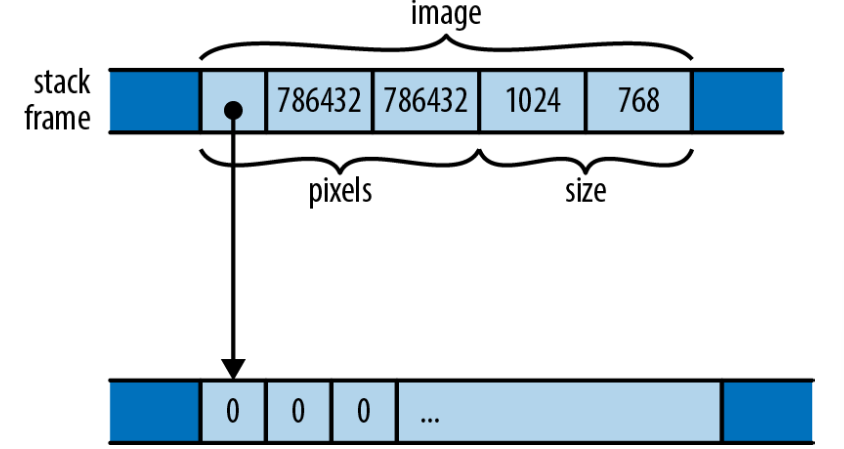
\includegraphics[width=0.8\textwidth]{../img/f9-1.png}
    \caption{一个\texttt{GrayscaleMap}结构体的内存布局}
    \label{f9-1}
\end{figure}

与C和C++不同,Rust对于如何在内存中布局结构体字段或元素没有任何确切的保证,这里的图只是展示了其中一种可能的排列。然而Rust确实保证了直接在结构体的内存块里存储字段的值。JavaScript、Python和Java将会把\texttt{pixels}和\texttt{size}值分别放在它们自己的堆上分配的内存块中,然后让\texttt{GrayscaleMap}的字段指向他们。而Rust会直接把\texttt{pixels}和\texttt{size}嵌入到\texttt{GrayscaleMap}值里。只有\texttt{pixels} vector持有的堆上分配的缓冲区保留着自己的块。

你可以使用\texttt{\#[repr(C)]}属性来要求Rust用一种与C和C++兼容的方式布局结构体。我们将会在\hyperref[ch23]{第23章}中详细介绍这些。

\section{使用\texttt{impl}定义方法}\label{method}

在本书中,我们已经在很多类型的值上调用过方法。我们使用\texttt{v.push(e)}把元素添加进vector,使用\texttt{v.len()}获取它的长度,使用\texttt{r.expect("msg")}检查\texttt{Result}的值是否是错误值,等等。你可以为你自己的结构体类型定义方法。与C++或Java那种直接出现在结构体定义内部的方式不同,Rust的方法在一个单独的\texttt{impl}块中定义。

一个\texttt{impl}块就是一些\texttt{fn}定义的结合,每一个函数都将成为这个结构体的一个方法。例如,这里我们定义了一个公有的结构体\texttt{Queue},然后为它定义了两个公有的方法:\texttt{push}和\texttt{pop}:
\begin{minted}{Rust}
    /// 一个先进先出的字符队列
    pub struct Queue {
        older: Vec<char>,   // 旧的元素,越旧越靠后
        younger: Vec<char>  // 新的元素,越新越靠后
    }

    impl Queue {
        /// 将一个字符添加到队列的尾部。
        pub fn push(&mut self, c: char) {
            self.younger.push(c);
        }

        /// 移出队列最前端的元素,如果有字符被移出就返回`Some(c)`,
        /// 否则如果队列为空就返回`None`。
        pub fn pop(&mut self) -> Option<char> {
            if self.older.is_empty() {
                if self.younger.is_empty() {
                    return None;
                }

                // 将新的元素都移动到旧的元素里,
                // 并且反转顺序。
                use std::mem::swap;
                swap(&mut self.older, &mut self.younger);
                self.older.reverse();
            }

            // 现在旧的元素保证不为空。Vec的pop方法
            // 已经返回了一个Option,因此不用再处理
            self.older.pop()
        }
    }
\end{minted}

在\emph{impl}块中定义的函数被称为\emph{关联函数},因为它们被关联到特定的类型。与之相反的是\emph{自由函数},也就是不在\texttt{impl}块中定义的函数。

Rust将调用方法的值作为第一个参数传给方法,它的参数名必须是\texttt{self}。因为\texttt{self}的类型很明显是\texttt{impl}块外面的结构体类型,或者是其引用,所以Rust允许你省略类型,用\texttt{self}、\texttt{\&self}、\texttt{\&mut self}分别作为\texttt{self: Queue}、\texttt{self: \&Queue}、\texttt{self: \&mut Queue}的缩写。如果你喜欢的话也可以使用非缩写的形式,但几乎所有的Rust代码都是用缩写形式。

在我们的示例中,\texttt{push}和\texttt{pop}方法中通过\texttt{self.older}和\texttt{self.younger}引用了\texttt{Queue}的字段。与C++或Java中“this”对象的成员直接在方法内可见不同,Rust方法中必须显式使用\texttt{self}来引用字段,这和Python方法中\texttt{self}的用法、JavaScript方法中\texttt{this}的用法类似。

因为\texttt{push}和\texttt{pop}需要修改\texttt{Queue},所以它们都以\texttt{\&mut self}传参。然而,当你调用这两个方法时,你不需要手动借用可变引用,普通的方法调用语法会自动进行隐式转换。因此有了这些定义之后,你可以像这样使用\texttt{Queue}:
\begin{minted}{Rust}
    let mut q = Queue { older: Vec::new(), younger: Vec::new() };

    q.push('0');
    q.push('1');
    assert_eq!(q.pop(), Some('0'));

    q.push('=');
    assert_eq!(q.pop(), Some('1'));
    assert_eq!(q.pop(), Some('='));
    assert_eq!(q.pop(), None);
\end{minted}

为了满足\texttt{push}方法的\texttt{self}参数要求,直接写\texttt{q.push(...)}会借用\texttt{q}的可变引用,就像你写了\texttt{(\&mut q).push(...)}一样。

如果一个方法不需要修改\texttt{self},那么你可以以共享引用获取参数。例如:
\begin{minted}{Rust}
    impl Queue {
        pub fn is_empty(&self) -> bool {
            self.older.is_empty() && self.younger.is_empty()
        }
    }
\end{minted}

方法调用表达式知道要借用哪一种引用:
\begin{minted}{Rust}
    assert!(q.is_empty());
    q.push('☉');
    assert!(!q.is_empty());
\end{minted}

或者,如果一个方法想获取\texttt{self}的所有权,它可以以值传递\texttt{self}:
\begin{minted}{Rust}
    impl Queue {
        pub fn split(self) -> (Vec<char>, Vec<char>) {
            (self.older, self.younger)
        }
    }
\end{minted}

调用这个\texttt{split}方法看起来和调用其他方法一样:
\begin{minted}{Rust}
    let mut q = Queue { older: Vec::new(), younger: Vec::new() };

    q.push('P');
    q.push('D');
    assert_eq!(q.pop(), Some('P'));
    q.push('X');

    let (older, younger) = q.split();
    // q现在是未初始化状态
    assert_eq!(older, vec!['D']);
    assert_eq!(younger, vec!['X']);
\end{minted}

但是注意,因为\texttt{split}以值获取\texttt{self},这会把\texttt{q}中的\texttt{Queue}值\emph{移动}走,导致\texttt{q}变为未初始化。因为\texttt{split}的\texttt{self}现在拥有了这个队列,因此它可以把两个单独的vector移动出来并返回给调用者。

有时,像这样以值传递\texttt{self},或者以引用传递都不能满足我们的需求,因此Rust还允许你通过智能指针类型传递\texttt{self}。

\subsection{以\texttt{Box}、\texttt{Rc}、\texttt{Arc}传递\texttt{Self}}

一个方法的\texttt{self}参数还可以是\texttt{Box<Self>}、\texttt{Rc<Self>}、\texttt{Arc<Self>}。这些方法只能在相应指针类型上调用。调用这些方法会传递指针的所有权。

你通常不需要这么做。一个以引用传递\texttt{self}的方法可以在任何智能指针类型上正常调用:
\begin{minted}{Rust}
    let mut bq = Box::new(Queue::new());

    // `Queue::push`接受一个`&mut Queue`,但`bq`是`Box<Queue>`。
    // 这没有问题:Rust在调用期间从`Box`借用了一个`&mut Queue`
    bq.push('■');
\end{minted}

对于方法调用和字段访问,Rust自动从智能指针类型例如\texttt{Box}、\texttt{Rc}和\texttt{Arc}借用一个引用,因此\texttt{\&self}和\texttt{\&mut self}通常总是正确的方法签名,再加上偶尔用到的\texttt{self}。

但如果这个方法的意图涉及管理指针的所有权呢?假设我们有一个像这样的节点组成的树,类似某种彻底简化的XML:
\begin{minted}{Rust}
    use std::rc::Rc;

    struct Node {
        tag: String,
        children: Vec<Rc<Node>>
    }

    impl Node {
        fn new(tag: &str) -> Node {
            Node {
                tag: tag.to_string(),
                children: vec![],
            }
        }
    }
\end{minted}

每一个节点都有一个tag来指示它是什么类型的节点,还有一个子节点的vector通过引用计数指针来允许共享,并让生命周期变得更灵活。

通常我们会实现一个方法让它向自己的列表中添加一个子节点,但现在让我们把角色颠倒过来,给\texttt{Node}实现一个把它自己添加到别的\texttt{Node}的子节点中的方法。我们可以写:
\begin{minted}{Rust}
    impl Node {
        fn append(self, parent: &mut Node) {
            parent.children.push(Rc::new(self));
        }
    }
\end{minted}

但这个方法并不能让人满意。这个方法调用了\texttt{Rc::new}来分配新的堆空间并且把\texttt{self}移动进去,但如果调用者已经有了一个\texttt{Rc<Node>},这些操作就都不是必须的:我们应该只递增引用计数然后把指针加到vector里。\texttt{Rc}的全部意义不就是实现共享吗?

我们可以这样写:
\begin{minted}{Rust}
    impl Node {
        fn append_to(self: Rc<Self>, parent: &mut Node) {
            parent.children.push(self);
        }
    }
\end{minted}

如果调用者已经是\texttt{Rc<Node>}类型,那它可以直接调用\texttt{append\_to},以值传递\texttt{Rc}:
\begin{minted}{Rust}
    let shared_node = Rc::new(Node::new("first"));
    shared_node.append_to(&mut parent);
\end{minted}

这会把\texttt{shared\_node}的所有权传递给方法:引用计数不会发生变化,也不会有新的内存分配。

如果调用者需要保留节点的指针以便之后使用,它可以首先克隆\texttt{Rc}再调用:
\begin{minted}{Rust}
    shared_node.clone().append_to(&mut parent);
\end{minted}

克隆\texttt{Rc}只会递增引用计数,没有堆分配或者拷贝。但当调用返回时\texttt{shared\_node}和\texttt{parent}\\
的子节点的vector现在指向同一个\texttt{Node}。

最后,如果调用者现在拥有一个\texttt{Node},那么它必须先创建一个\texttt{Rc}再调用方法:
\begin{minted}{Rust}
    let owned = Node::new("owned directly");
    Rc::new(owned).append_to(&mut parent);
\end{minted}

把\texttt{append\_to}方法的签名设为\texttt{Rc<Self>}可以让调用者知道\texttt{Node}的需求。然后调用者可以用最小化内存分配和引用计数调整的方式来调用:
\begin{itemize}
    \item 如果可以传递\texttt{Rc}的所有权,就直接在指针上调用。
    \item 如果需要保留\texttt{Rc}的所有权,就递增引用计数后再调用。
    \item 如果只拥有\texttt{Node},那么必须先调用\texttt{Rc::new}来分配堆空间然后把\texttt{Node}移动进去。因为\texttt{parent}必须通过\texttt{Rc<Node>}指针引用它的子节点,所以这一步最终肯定是必须的。
\end{itemize}

再重复一遍,对于大多数方法,\texttt{\&self}、\texttt{\&mut self}、和\texttt{self}(以值传参)就能满足你的需求。但如果一个方法的目的是影响值的所有权,使用其他指针类型的\texttt{self}可能是正确的选择。

\subsection{类型关联函数}
\texttt{impl}块里定义的函数也可以没有\texttt{self}参数。这些参数仍然和类型关联,因为它们也是在\texttt{impl}块中定义的。但它们不是方法,因为它们没有\texttt{self}参数。为了将它们和方法区别开来,我们称它们为\emph{类型关联函数}。

它们通常用于提供构造函数,例如:
\begin{minted}{Rust}
    impl Queue {
        pub fn new() -> Queue {
            Queue { older: Vec::new(), younger: Vec::new() }
        }
    }
\end{minted}

为了使用这个函数,我们通过\texttt{Queue::new}来引用它:类型名+双冒号+函数名。现在我们的示例代码变得更加简洁:
\begin{minted}{Rust}
    let mut q = Queue::new();

    q.push('*');
    ...
\end{minted}

Rust的传统是构造函数都叫\texttt{new},我们已经见过了\texttt{Vec::new}、\texttt{Box::new}、\texttt{HashMap::new},等等。但\texttt{new}这个名字本身并没有什么特殊的地方。它并不是关键字,而且一个类型经常还有其他名字的关联函数作为构造函数,例如\texttt{Vec::with\_capacity}。

尽管一个类型可以有很多个分开的\texttt{impl}块,但它们必须在定义类型的那个crate中。然而,Rust确实允许你将自己定义的方法附加到其他类型,我们将在\hyperref[ch11]{第11章}介绍怎么做到这一点。

如果你习惯写C++或Java,你可能会觉得将类型的方法和定义分离开来很奇怪,但这么做确实有以下优势:
\begin{itemize}
    \item 你总是能很容易的找到一个类型的数据成员。在很大的C++类定义中,你可能需要浏览几百行成员成员函数的定义来确保你没有遗漏数据成员。而在Rust中,所有数据成员都在一个地方。
    \item 尽管我们可以很容易想象把方法定义添加到命名字段结构体的定义中,但类元组结构体和类单元结构体却不是这样。将方法拿出来放在一个\texttt{impl}块中可以让这三种结构体共用唯一一种语法。事实上,Rust还使用这套语法为不是结构体的类型定义方法,例如\texttt{enum}结构体和基本类型例如\texttt{i32}。(任何类型都可以有方法的事实是Rust中不使用术语\emph{对象},而是更喜欢把一切称为\emph{值}的原因之一。)
    \item 同样的\texttt{impl}语法还可以很容易地用于实现trait,我们将在\hyperref[ch11]{第11章}中介绍。
\end{itemize}

\section{关联常量}
Rust的类型系统还采用了C\#和Java等语言中的一个特性,就是关联到类型而不是关联到类型实例的值。在Rust中,它们被称为\emph{关联常量}。

正如它的名字一样,关联常量是常量值。它们通常用来表示某一个类型中使用最广泛的值。例如,你可以定义一个二维的向量用于线性代数,并为它定义一个关联的单位向量:
\begin{minted}{Rust}
    pub struct Vector2 {
        x: f32,
        y: f32,
    }

    impl Vector2 {
        const ZERO: Vector2 = Vector2 { x: 0.0, y: 0.0 };
        const UNIT: Vector2 = Vector2 { x: 1.0, y: 0.0 };
    }
\end{minted}

这些值被关联到类型本身,你可以在不创建\texttt{Vector2}的实例的情况下使用它们。和类型关联方法一样,引用它们的方法是类型的名称再加上它们的名称:
\begin{minted}{Rust}
    let scaled = Vector2::UNIT.scaled_by(2.0);
\end{minted}

关联常量的类型并不一定必须是它关联的类型,我们可以使用这个特性来给类型添加ID或者名称。例如,如果有几个和\texttt{Vector2}很像的类型需要写入到文件里,然后加载到内存中,那么关联常量可以为写入的数据添加名称或数字ID,这样之后可以据此辨识出类型:
\begin{minted}{Rust}
    impl Vector2 {
        const NAME: &'static str = "Vector2";
        const ID: u32 = 18;
    }
\end{minted}

\section{泛型结构体}\label{GenStruct}

我们之前的\texttt{Queue}定义并不能令人满意:它被用来存储字符,但它却没有任何和字符相关的方法。如果我们要定义另一个存储\texttt{String}值的结构体,那么除了\texttt{char}要换成\texttt{String}之外,剩下的代码完全相同。重复定义将会浪费时间。

幸运的是,Rust的结构体可以是\emph{泛型}的,这意味着它们的定义只是一个模板,你可以把任何类型塞进去。例如,这里有一个可以存储任何类型的值的\texttt{Queue}的定义:
\begin{minted}{Rust}
    pub struct Queue<T> {
        older: Vec<T>,
        younger: Vec<T>
    }
\end{minted}

你可以将\texttt{Queue<T>}中的\texttt{<T>}读作“对于任意类型\texttt{T}”。因此这个定义读作“对于任意类型\texttt{T},一个\texttt{Queue<T>}有两个\texttt{Vec<T>}类型的字段。”例如,在\texttt{Queue<String>}中,\texttt{T}是\texttt{String},所以\texttt{older}和\texttt{younger}的类型都是\texttt{Vec<String>}。在\texttt{Queue<char>}中\texttt{T}是\texttt{char},我们就得到了一个和一开始的\texttt{char}类型特定的定义完全相同的结构体。事实上,\texttt{Vec}本身就是一个用这种方式定义的泛型结构体。

在泛型结构体的定义中,<尖括号>里的类型名被称为\emph{类型参数}。一个泛型结构体的\texttt{impl}块看起来像这样:
\begin{minted}{Rust}
    impl<T> Queue<T> {
        pub fn new() -> Queue<T> {
            Queue { older: Vec::new(), younger: Vec::new() }
        }

        pub fn push(&mut self, t: T) {
            self.younger.push(t);
        }

        pub fn is_empty(&self) -> bool {
            self.older.is_empty() && self.younger.is_empty()
        }

        ...
    }
\end{minted}

你可以将\texttt{impl<T> Queue<T>}这一行读作“对于任意类型\texttt{T},有一些\texttt{Queue<T>}可用的关联方法”。然后,你可以在关联函数的定义中将类型参数\texttt{T}用作一个类型。

这种语法看起来好像有些重复,但\texttt{impl<T>}能更清晰地表达出\texttt{impl}块覆盖了任意的类型\texttt{T},这能将它和为特定种类的\texttt{Queue}编写的\texttt{impl}块区分开来,例如:
\begin{minted}{Rust}
    impl Queue<f64> {
        fn sum(&self) -> f64 {
            ...
        }
    }
\end{minted}

这个\texttt{impl}块头读作“这里有一些\texttt{Queue<f64>}特定的关联方法”。这样就给\texttt{Queue<f64>}添加了一个\texttt{sum}方法,而其它种类的\texttt{Queue}并没有这个方法。

我们已经在之前的代码中使用过Rust的\texttt{self}参数的缩写形式。这里\texttt{Queue<T>}如果写出类型显得有些啰嗦。作为另一种缩写,每一个\texttt{impl}块,不管是不是泛型的,都定义了特殊的类型参数\texttt{Self}(注意\texttt{大驼峰}风格的名称)来表示我们要添加方法的类型。在之前的代码中,\texttt{Self}将是\texttt{Queue<T>},因此我们可以进一步简化\texttt{Queue::new}的定义:
\begin{minted}{Rust}
    pub fn new() -> Self {
        Queue { older: Vec::new(), younger: Vec::new() }
    }
\end{minted}

你可能已经注意到了,在\texttt{new}的函数体内,我们不需要在构造表达式中写出类型参数,简单地写\texttt{Queue \{ ... \}}就足够了。这是因为Rust的类型推导发挥了作用:因为函数的返回值类型只能有一种可能,就是\texttt{Queue<T>},所以Rust会自动为我们提供参数。然而,你必须总是在函数签名和类型定义中指明类型参数。Rust不会推断它们,相反,它将这些已知的类型作为基础来推断那些函数体内的类型。

\texttt{Self}也可以用于这种方式:我们可以写\texttt{Self \{ ... \}}。你觉得哪种形式更容易理解就可以用哪种。

对于关联函数的调用,你可以显式地使用\texttt{::<>(涡轮鱼)}注解来提供类型参数:
\begin{minted}{Rust}
    let mut q = Queue::<char>::new();
\end{minted}

但在实践中,通常可以让Rust自动帮你推断类型:
\begin{minted}{Rust}
    let mut q = Queue::new();
    let mut r = Queue::new();

    q.push("CAD");      // 显然是Queue<&'static str>
    r.push(0.74);       // 显然是Queue<f64>

    q.push("BTC");      // 比特币/USD,2019年6月 
    r.push(13764.0);    
\end{minted}

事实上,这正是整本书中我们使用\texttt{Vec}的方式。

并不只有结构体可以是泛型的。枚举也可以有类型参数,语法也非常的相似。我们将在\nameref{enum}一节中详细介绍。

\section{有生命周期参数的结构体}

正如我们在\nameref{refstruct}一节中讨论过的一样,如果一个结构体类型中包含引用,你必须指明那些引用的生命周期。例如,这里有一个存储切片中最大和最小元素的引用的结构体:
\begin{minted}{Rust}
    struct Extrema<'elt> {
        greatest: &'elt i32,
        least: &'elt i32
    }
\end{minted}

之前,我们建议你将类似\texttt{struct Queue<T>}的声明看作是对于任意类型\texttt{T},你都可以构建一个\texttt{Queue<T>}来存储该类型。类似的,你可以将\texttt{struct Extrema<'elt>}看作对于任意生命周期\texttt{'elt},你都可以构建一个\texttt{Extrema<'elt>}来存储生命周期为\texttt{'elt}的引用。

这里有一个函数来扫描一个切片并返回一个指向其中元素的\texttt{Extrema}值:
\begin{minted}{Rust}
    fn find_extrema<'s>(slice: &'s [i32]) -> Extrema<'s> {
        let mut greatest = &slice[0];
        let mut least = &slice[0];

        for i in 1..slice.len() {
            if slice[i] < *least    { least     = &slice[i]; }
            if slice[i] > *greatest { greatest  = &slice[i]; }
        }
        Extrema { greatest, least }
    }
\end{minted}

这里,\texttt{find\_extrema}借用了\texttt{slice}的元素。因为\texttt{slice}的生命周期是\texttt{'s},所以我们返回的\texttt{Extrema}结构体中的引用的生命周期也是\texttt{'s}。Rust总是会为调用推断生命周期参数,因此调用\texttt{find\_extrema}并不需要提到它们:
\begin{minted}{Rust}
    let a = [0, -3, 0, 15, 48];
    let e = find_extrema(&a);
    assert_eq!(*e.least, -3);
    assert_eq!(*e.greatest, 48);
\end{minted}

因为返回值和参数使用相同的生命周期非常常见,所以当只有一种可能时Rust允许我们省略生命周期。我们还可以在不改变含义的情况下将\texttt{find\_extrema}的签名写成这样:
\begin{minted}{Rust}
    fn find_extrema(slice: &[i32]) -> Extrema {
        ...
    }
\end{minted}

诚然,我们也\emph{可能}是想返回\texttt{Extrema<'static>},但这并不是通常的情况。Rust只为通常的情况提供了一个缩写。

\section{为结构体类型派生常见的trait}

可以非常简单地定义一个结构体:
\begin{minted}{Rust}
    struct Point {
        x: f64,
        y: f64
    }
\end{minted}

然而,如果你真的开始使用这个\texttt{Point}类型,你将很快发现它使用起来很痛苦。按照上面的写法,\texttt{Point}既不能拷贝也不能克隆。你不能用\texttt{println!("\{:?\}", point);}打印它,它也不支持\texttt{==}和\texttt{!=}运算符。

在Rust中这些特性都有一个名字——\texttt{Copy}、\texttt{Clone}、\texttt{Debug}、\texttt{PartialEq}。它们被称为\emph{trait}。在\hyperref[ch11]{第11章}中,我们将展示如何为你自己的结构体手动实现trait。但这个例子中出现的标准trait,以及其它一些trait,你不需要手动实现它们,除非你想要一些自定义行为。Rust可以自动为你实现它们。只需要为结构体添加\texttt{\#[derive]}属性:
\begin{minted}{Rust}
    #[derive(Copy, Clone, Debug, PartialEq)]
    struct Point {
        x: f64,
        y: f64
    }
\end{minted}

这些trait中的任何一个都可以自动实现,前提是这个结构体的所有字段都实现了那个trait。我们可以要求Rust为\texttt{Point}派生\texttt{PartialEq},是因为它的两个字段都是\texttt{f64}类型,这个类型已经实现了\texttt{PartialEq}。

Rust还可以派生\texttt{PartialOrd},它可以支持比较运算符\texttt{<}、\texttt{>}、\texttt{<=}和\texttt{>=}。我们没有这么做,是因为比较两个点来判断其中一个是否“小于”另一个是一件很奇怪的事。因此我们选择让\texttt{Point}值不支持那些比较运算符。像这样的情况也是Rust让我们自己写\texttt{\#[derive]}属性而不是直接自动派生所有可用的trait的原因之一。另一个原因是实现一个trait将自动变为公有的特性。因此可复制性、可克隆性等都将是结构体公共API的一部分,应该慎重选择。

我们将在\hyperref[ch13]{第13章}详细介绍Rust的标准trait并解释哪些可以用\texttt{\#[derive]}自动实现。

\section{内部可变性}\label{intermut}

可变性和其他东西一样:如果限制太过宽松就会导致问题,但你又总是希望它能放宽一点。例如,假设你的蜘蛛机器人控制系统是一个中心化的结构体\texttt{SpiderRobot},这个结构体里包含设置和I/O处理。当机器人启动时它的值就被初始化,并且永远不会改变:
\begin{minted}{Rust}
    pub struct SpiderRobot {
        species: String,
        web_enabled: bool,
        leg_devices: [fd::FileDesc; 8],
        ...
    }
\end{minted}

机器人的每一个主要系统都由一个不同的结构体处理,这些结构体都有一个指向那个\texttt{SpiderRobot}值的指针:
\begin{minted}{Rust}
    use std::rc::Rc;

    pub struct SpiderSenses {
        robot: Rc<SpiderRobot>, // <-- 指向设置和I/O的指针
        eyes: [Camera; 32],
        motion: Accelerometer,
        ...
    }
\end{minted}

控制织网、捕食、毒液流动等的结构体都有一个\texttt{Rc<SpiderRobot>}智能指针。回顾一下,\texttt{Rc}代表\hyperref[rc]{引用计数},、\texttt{Rc}中的值总是共享的因此总是不可变的。

现在假设你想使用标准的\texttt{File}类型给\texttt{SpiderRobot}结构体添加一点日志功能。那么就会有一个问题:\texttt{File}值必须是\texttt{mut}的。所有写入它的函数都需要\texttt{mut}引用。

这种情况经常出现。我们需要的是一个不可变(\texttt{SpiderRobot}结构体)的值内有一小部分数据可变(一个\texttt{File})。这被称为\emph{内部可变性}。Rust为此提供了几种方式,这一节中我们将讨论最直观的两种类型:
\texttt{Cell<T>}和\texttt{RefCell<T>},这两个类型都在\texttt{std::cell}模块中。

\texttt{Cell<T>}结构体只包含单个私有的类型\texttt{T}的值。\texttt{Cell}唯一特殊的地方是即使你没有对\texttt{Cell}自身的\texttt{mut}访问权限,也可以访问和修改它里面的字段值:

\codeentry{Cell:new(value)}
\hangparagraph{创建一个新的\texttt{Cell},将给定的\texttt{value}移动进去。}

\codeentry{cell.get()}
\hangparagraph{返回一个\texttt{cell}中值的拷贝}

\codeentry{cell.set(value)}
\hangparagraph{将给定的值\texttt{value}存储在\texttt{cell}中,丢弃掉之前存储的值。这个方法以非\texttt{mut}引用获取\texttt{self}参数:}
\begin{minted}{Rust}
    fn set(&self, value: T) // 注意:不是`&mut self`
\end{minted}
\hangparagraph{显然,这和普通的\texttt{set}方法不同。到目前为止,Rust告诉我们如果想要修改数据就需要\texttt{mut}访问权限。但同样的道理,这一处不同的细节就是\texttt{Cell}全部的精髓。它们是一种安全地扭曲不可变性规则的方式——既不多、也不少。}

\texttt{Cell}还可以有一些其他的方法,你可以在\href{https://doc.rust-lang.org/std/cell/struct.Cell.html}{它的文档}中查阅。

如果你想给你的\texttt{SpiderRobot}添加一个简单的计数器,那么使用\texttt{Cell}将会很方便。你可以写:
\begin{minted}{Rust}
    use std::cell::Cell;

    pub struct SpiderRobot {
        ...
        hardware_error_count: Cell<u32>,
        ...
    }
\end{minted}

即使是\texttt{SpiderRobot}的非\texttt{mut}方法也可以使用\texttt{.get()}和\texttt{.set()}来访问\texttt{u32}:
\begin{minted}{Rust}
    impl SpiderRobot {
        /// 错误计数加一
        pub fn add_hardware_error(&self) {
            let n = self.hardware_error_count.get();
            self.hardware_error_count.set(n + 1);
        }

        /// 如果有硬件错误的话返回真
        pub fn has_hardware_errors(&self) -> bool {
            self.hardware_error_count.get() > 0
        }
    }
\end{minted}

这非常简单,但并不能解决我们的日志问题。\texttt{Cell}\emph{不能}让你调用内含值的\texttt{mut}方法,因为\texttt{.get()}方法返回的是单元里值的拷贝,所以它只能用于实现了\hyperref[copy]{\texttt{Copy} trait}的类型。为了实现日志功能,我们需要一个可变的\texttt{File},而\hyperref[file]{\texttt{File}}不可拷贝。

这个例子中正确的工具是\texttt{RefCell}。类似于\texttt{Cell<T>},\texttt{RefCell<T>}也是一个包含单个\texttt{T}类型的值的泛型类型。和\texttt{Cell}不同的是,\texttt{RefCell}支持借用内部的\texttt{T}类型的值:

\codeentry{RefCell::new(value)}
\hangparagraph{创建一个新的\texttt{RefCell},把\texttt{value}移动进去。}

\codeentry{ref\_cell.borrow()}
\hangparagraph{返回一个\texttt{Ref<T>},它本质上是\texttt{ref\_cell}里存储的值的一个共享引用。}
\hangparagraph{如果里面的值已经有可变借用了,这个方法会panic。}

\codeentry{ref\_cell.borrow\_mut()}
\hangparagraph{返回一个\texttt{RefMut<T>},它本质上是\texttt{ref\_cell}里存储的值的一个可变引用。}
\hangparagraph{如果里面的值已经被借用了,这个方法会panic。}

\codeentry{ref\_cell.try\_borrow(), ref\_cell.try\_borrow\_mut()}
\hangparagraph{与\texttt{borrow()}和\texttt{borrow\_mut()}的功能一样,但返回一个\texttt{Result}。当值已经有可变借用/被借用时,它们不panic,而是返回一个\texttt{Err}值。}

同样的,\texttt{RefCell}还有一些其它方法,你可以在\href{https://doc.rust-lang.org/std/cell/struct.RefCell.html}{它的文档}中查阅。

只有当你尝试打破Rust中\texttt{mut}引用必须是独占引用的规则时这两个方法才会panic。例如,这样将会panic:
\begin{minted}{Rust}
    use std::cell::RefCell;

    let ref_cell: RefCell<String> = RefCell::new("hello".to_string());

    let r = ref_cell.borrow();  // ok,返回一个Ref<String>
    let count = r.len();        // ok, 返回"hello".len()
    assert_eq!(count, 5);       

    let mut w = ref_cell.borrow_mut(); // panic:已经被借用了
    w.push_str(" world");
\end{minted}

为了避免panic,你可以把这两个借用放进单独的块里。这样的话,\texttt{r}会在你尝试借用\texttt{w}之前被drop。

这和普通引用的工作方式很像。唯一的不同在于普通的情况下,当你尝试借用一个变量的引用,Rust会在\emph{编译期}确保你必须安全地使用引用。如果检查失败了,你会得到一个编译期错误。\texttt{RefCell}使用运行时检查来执行同样的规则。如果你尝试打破规则,你会得到一个panic(或者使用\texttt{try\_borrow}和\texttt{try\_borrow\_mut}时会得到一个\texttt{Err})。

现在我们已经准备好用\texttt{RefCell}来完善我们的\texttt{SpiderRobot}了:
\begin{minted}{Rust}
    pub struct SpiderRobot {
        ...
        log_file: RefCell<File>,
        ...
    }

    impl SpiderRobot {
        /// 向日志文件中写入一行。
        pub fn log(&self, message: &str) {
            let mut file = self.log_file.borrow_mut();
            // `writeln!`和`println!`很像,
            // 但会把字符串写入到给定的文件中。
            writeln!(file, "{}", message).unwrap();
        }
    }
\end{minted}

变量\texttt{file}的类型是\texttt{RefMut<File>}。它的使用方式就像\texttt{File}的可变引用一样。有关写入文件的细节,见\hyperref[ch18]{第18章}。

Cell很容易使用。虽然必须调用\texttt{.get()}和\texttt{.set()}或者\texttt{.borrow()}和\texttt{.borrow\_mut()}有点麻烦,但那只是我们扭曲可变性规则的代价。还有一些不是很明显但却更严重的问题:Cell——和任何包含了它们的类型——都不是线程安全的。因此Rust\hyperref[threadsafe]{不允许}多个线程直接访问它们。我们将在\hyperref[ch19]{第19章}中讨论到\nameref{mutex}、\nameref{atomic}和\nameref{globalvar}时介绍多线程中的内部可变性。

不管一个结构体有命名字段还是类元组结构体,它都是一些其他值的聚合体:如果我有一个\texttt{SpiderSenses}结构体,那么我就有一个指向共享的\texttt{SpiderRobot}结构体的\texttt{Rc}指针、同时还有了eyes、accelerometer等等。因此结构体的本质是单词“和(and)”:我有一个X\emph{和(and)}一个Y。但是否有另一种类型用于单词“或(or)”呢?换句话说,当你有了一个这种类型的值时,你有了一个X\emph{或(or)}一个Y?这样的类型太有用了以至于它们在Rust中无处不在,它们就是我们下一章要讨论的主题。

    \chapter{枚举与模式}\label{ch10}

\emph{Surprising how much computer stuff makes sense viewed as tragic deprivation of sum types (cf. deprivation of lambdas).}

\begin{flushright}
    ——Graydon Hoare
\end{flushright}

这一章的第一个话题将是一个古老的、强有力的、可以帮你在短期内完成很多工作的(有代价地)、并且在许多语言中以不同的名字广为人知的特性。但它并不是魔鬼。而是一种用户自定义的数据类型,它是ML和Haskell程序员们熟知的和类型、也是互斥的联合、还是代数数据类型。在Rust中,它们被称为\emph{枚举(enumerations)},或者简写为\emph{enum}。和魔鬼不同的是,它们非常安全、索取的代价也很小。

C++和C\#都有枚举,你可以使用它们来定义自己的类型,这种类型的取值范围是一些命名常量的集合。例如,你可能定义过一个叫\texttt{Color}的类型,取值范围为\texttt{Red}、\texttt{Orange}、\texttt{Yellow}等等。这种枚举在Rust中也能工作,但Rust进一步扩展了枚举。一个Rust枚举可以包含数据,包括多种不同类型的数据。例如,Rust的\texttt{Result<String, io::Error}类型是一个枚举;这样一个值要么是一个包含\texttt{String}的\texttt{Ok}值要么是一个包含\texttt{io::Error}的\texttt{Err}值。这就超出了C++和C\#中枚举的能力。它更像C中的\texttt{union}——但和联合不同的是,Rust的枚举是类型安全的。

枚举适用于一个值有多种可能的情况。使用它们的“代价”是你必须使用模式匹配来安全地访问数据,这也是我们这一章中的第二个话题。

如果你使用过Python的解包或者JavaScript中的解构,那你可能觉得模式也很熟悉,但Rust同样扩展了模式。Rust的模式有点像匹配数据的正则表达式。它们被用来测试一个值是否具有特定的期望的形态。它们可以一次从结构体或这元组中提取出多个字段存入局部变量。并且和正则表达式类似,它们很简洁,通常只用单行代码就能完成任务。

这一章将以枚举的基础开始,展示数据怎么被关联到枚举选项以及枚举是怎么存储在内存中的。然后我们会展示Rust的模式和\texttt{match}表达式如何简洁地指定基于枚举、结构体、数组、切片的逻辑。模式也可以包含引用、move和\texttt{if}条件,这让它们的功能更加强大。

\section{枚举}\label{enum}

简单的C风格枚举非常直观:
\begin{minted}{Rust}
    enum Ordering {
        Less,
        Equal,
        Greater,
    }
\end{minted}

这里声明了一个有三个可能的值的\texttt{Ordering}类型,这些值被称为\emph{variant}或者\emph{constructor}:\texttt{Ordering::Less}、\texttt{Ordering::Equal}、\texttt{Ordering::Greater}。这个枚举是标准库的一部分,因此Rust代码可以导入它:
\begin{minted}{Rust}
    use std::cmp::Ordering;

    fn compare(n: i32, m: i32) -> Ordering {
        if n < m {
            Ordering::Less
        } else if n > m {
            Ordering::Greater
        } else {
            Ordering::Equal
        }
    }
\end{minted}

或者它的所有constructor:
\begin{minted}{Rust}
    use std::cmp::Ordering::{self, *};  // `*`意思是导入所有的子item

    fn compare(n: i32, m: i32) -> Ordering {
        if n < m {
            Less
        } else if n > m {
            Greater
        } else {
            Equal
        }
    }
\end{minted}

导入constructor之后,我们可以写\texttt{Less}来代替\texttt{Ordering::Less}等,但因为这样不够明显,因此一般认为\emph{不要}导入它们式更好的风格,除非它能是你的代码的可读性更强。

为了导入一个在当前模块中声明的枚举的constructor,可以使用\texttt{self}:
\begin{minted}{Rust}
    enum Pet {
        Orca,
        Giraffe,
        ...
    }

    use self::Pet::*;
\end{minted}

在内存中,C风格的枚举值被存储为整数。有时告诉Rust使用哪些整数会很有用:
\begin{minted}{Rust}
    enum HttpStatus {
        Ok = 200,
        NotModified = 304,
        NotFound = 404,
        ...
    }
\end{minted}

否则,Rust会从0开始自动分配值。

默认情况下,Rust用能容纳所有值的最小的内建整数类型来存储C风格枚举。大多数情况下都是一个单独的字节:
\begin{minted}{Rust}
    use std::mem::size_of;
    assert_eq!(size_of::<Ordering>(), 1);
    assert_eq!(size_of::<HttpStatus>(), 2); // 404不能存储在u8中
\end{minted}

你可以通过添加\texttt{\#[repr]}属性来覆盖Rust选择的内存表示方式。更多的细节见“\nameref{repr}”。

将C风格的枚举转换为整数是允许的:
\begin{minted}{Rust}
    assert_eq!(HttpStatus::Ok as i32, 200);
\end{minted}

然而,反过来把整数转换为枚举是不允许的。和C和C++不同,Rust保证枚举的值只能是\texttt{enum}生命中列出的值之一。未经检查的从整数类型到枚举类型的转换会打破这种保证,所以它是不允许的。你可以写出你自己的带检查的版本:
\begin{minted}{Rust}
    fn http_status_from_u32(n: u32) -> Option<HttpStatus> {
        match n {
            200 => Some(HttpStatus::Ok),
            304 => Some(HttpStatus::NotModified),
            404 => Some(HttpStatus::NotFound),
            ...
            _ => None,
        }
    }
\end{minted}

或者使用\href{https://crates.io/crates/enum_primitive}{\texttt{enum\_primitive}} crate。它包含一个宏可以为你自动生成这种类型的转换代码。

和结构体一样,编译器也可以为你自动生成类似\texttt{==}运算符这样的特性,但你需要显式地要求这样:
\begin{minted}{Rust}
    #[derive(Copy, Clone, Debug, PartialEq, Eq)]
    enum TimeUnit {
        Seconds, Minutes, Hours, Days, Months, Years,
    }
\end{minted}

枚举也和结构体一样可以拥有方法:
\begin{minted}{Rust}
    impl TimeUnit {
        /// 返回该时间单位的复数名词。
        fn plural(self) -> &'static str {
            match self {
                TimeUnit::Seconds => "seconds",
                TimeUnit::Minutes => "minutes",
                TimeUnit::Hours => "hours",
                TimeUnit::Days => "days",
                TimeUnit::Months => "months",
                TimeUnit::Years => "years",
            }
        }

        /// 返回该时间单位的单数名词。
        fn singular(self) -> &'static str {
            self.plural().trim_end_matches('s')
        }
    }
\end{minted}

C风格的枚举就这么多内容了。Rust中最有趣的一类枚举是那些带有数据的枚举。我们将展示这些枚举如何存储在内存中、如何通过添加类型参数将它们变为泛型的,以及如何通过枚举构建复杂的数据结构。

\subsection{带有数据的枚举}

一些程序总是需要显示完整的日期和时间,并且精确到毫秒。但对于大多数程序,显示大概的时间范围会更加友好,例如“两个月以前”。我们可以用之前定义的枚举编写一个新的枚举来实现这一点:
\begin{minted}{Rust}
    /// 一个故意舍入的时间戳,因此我们的程序会显示“6个月以前”
    /// 而不是“February 9, 2016, at 9:49 AM”。
    #[derive(Copy, Clone, Debug, PartialEq)]
    enum RoughTime {
        InThePast(TimeUnit, u32),
        JustNow,
        InTheFuture(TimeUnit, u32),
    }
\end{minted}

这个枚举中的两个variant,即\texttt{InThePast}和\texttt{InTheFuture}都有参数。这些被称为\emph{tuple variant}。就像类元组结构体一样,它们的constructor是创建新的\texttt{RoughTime}值的函数:
\begin{minted}{Rust}
    let four_score_and_seven_years_ago =
        RoughTime::InThePast(TimeUnit::Years, 4 * 20 + 7);

    let three_hours_from_now =
        RoughTime::InTheFuture(TimeUnit::Hours, 3);
\end{minted}

枚举也可以有\emph{struct variant},它们和普通的结构体一样拥有命名字段:
\begin{minted}{Rust}
    enum Shape {
        Sphere { center: Point3d, radius: f32 },
        Cuboid { corner1: Point3d, corner2: Point3d },
    }

    let unit_sphere = Shape::Sphere {
        center: ORIGIN,
        radius: 1.0,
    };
\end{minted}

总的来说,Rust有三种枚举variant,分别对应我们在上一章中展示的三种结构体。没有数据的variant对应类单元结构体。元组variant对应类元组结构体。结构体variant对应有花括号和命名字段的结构体。一个枚举可以同时有这三种variant:
\begin{minted}{Rust}
    enum RelationshipStatus {
        Single,
        InARelationship,
        ItsComplicated(Option<String>),
        ItsExtremelyComplicated {
            car: DifferentialEquation, 
            cdr: EarlyModernistPoem,
        },
    }
\end{minted}

所有种类的constructor都和枚举自身有相同的可见性。

\subsection{内存中的枚举}

在内存中,带有数据的枚举被存储为一个很小的整数\emph{标签(tag)},加上一块足够存储所有variant中最大的那个的内存。标签字段是Rust内部要使用的,它表示是哪一个constructor创建了这个值,进而得知这个值有哪些字段。

在Rust 1.50中,\texttt{RoughTime}存储为8个字节,如\hyperref[f10-1]{图10-1}所示。

\begin{figure}[htbp]
    \centering
    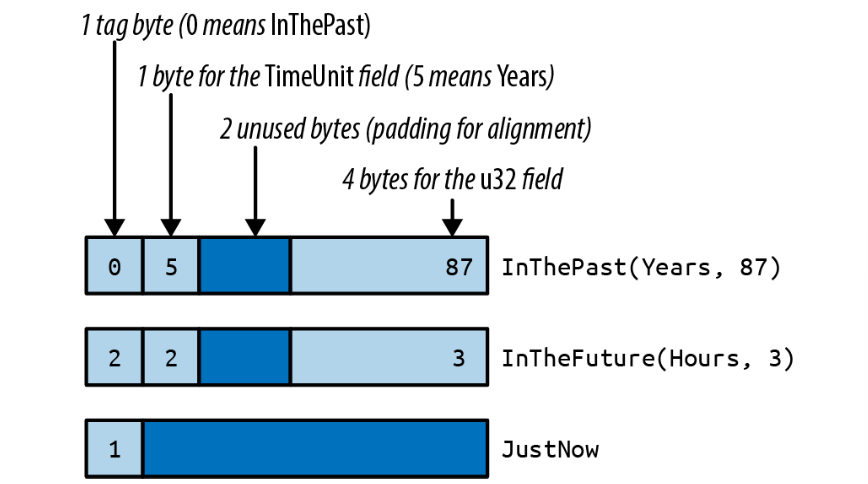
\includegraphics[width=0.9\textwidth]{../img/f10-1.png}
    \caption{内存中的\texttt{RoughTime}值}
    \label{f10-1}
\end{figure}

对于枚举的布局Rust不做任何保证。然而,为了给将来的优化留下余地,在一些情况下它可能会用比图中所示更加高效的方式包装一个枚举。例如,一些泛型结构体可以不用标签存储,我们稍后会讲到它。

\subsection{使用枚举实现富数据结构}

枚举在实现树形结构时也很有用。例如,假设一个Rust程序要处理任意的Json数据。在内存中,任何Json文档都可以被表示为一个这种Rust类型的值:
\begin{minted}{Rust}
    use std::collections::HashMap;

    enum Json {
        Null,
        Boolean(bool),
        Number(f64),
        String(String),
        Array(Vec<Json>),
        Object(Box<HashMap<String, Json>>),
    }
\end{minted}

与Rust代码相比,用英文来解释这个数据结构也不会再有太大的改进了。JSON标准定义了可以出现在JSON文档中的数据类型:\texttt{null}、布尔值、数字、字符串、JSON值的数组、以及带有字符串键和JSON值的对象。这个\texttt{Json}枚举简单地列出了这些类型。

这并不是一个假想的例子。你可以在\texttt{serde\_json} crate中找到一个非常相似的枚举,它是一个用于Rust结构体序列化的库,也是crates.io上下载次数最多的crate之一。

用于表示\texttt{Object}的\texttt{HashMap}外层的\texttt{Box}只是为了让\texttt{Json}值更加紧凑。在内存中,\texttt{Json}类型的值将占据4个机器字。\texttt{String}和\texttt{Vec}都是3个字,Rust会再添加一个字节的标签,再加上对齐所以总共是4个字。\texttt{Null}和\texttt{Boolean}值没有足够的数据利用全部的空间,但所有的\texttt{Json}值大小必须相同,因此这时多余的空间就被浪费了。\hyperref[f10-2]{图10-2}展示了一些示例的\texttt{Json}值在内存中的实际视图。

\begin{figure}[htbp]
    \centering
    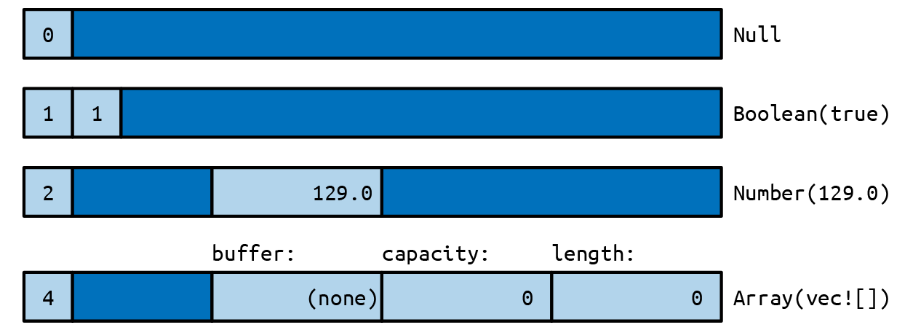
\includegraphics[width=0.8\textwidth]{../img/f10-2.png}
    \caption{内存中的\texttt{Json}值}
    \label{f10-2}
\end{figure}

一个\texttt{HashMap}会更大如果我们一定要在每一个\texttt{Json}值中给它留出空间,它们将会变得更大,也就是8个字。但\texttt{Box<HashMap>}是单个字:它只是一个指向堆上分配的数据的指针。我们甚至可以通过装箱更多的字段来让\texttt{Json}变得更加紧凑。

这里优秀的地方在于,我们如此简单的就完成了这一切。如果是在C++中,可能要写一个这样的一个类才行:
\begin{minted}{Rust}
    class JSON {
    private:
        enum Tag {
            Null, Boolean, Number, String, Array, Object
        };
        union Data {
            bool boolean;
            double number;
            shared_ptr<string> str;
            shared_ptr<vector<JSON>> array;
            shared_ptr<unordered_map<string, JSON>> object;

            Data() {}
            ~Data() {}
            ...
        };
        
        Tag tag;
        Data data;
    
    public:
        bool is_null() const { return tag == Null; }
        bool is_boolean const { return tag == Boolean; }
        bool get_boolean() const {
            assert(is_boolean());
            return data.boolean;
        }
        void set_boolean(bool value) {
            this->~JSON();  // 清除string/array/object值
            tag = Boolean;
            data.boolean = value;
        }
        ...
    };
\end{minted}

30行代码,我们才刚刚开始。这个类还需要构造函数、析构函数、一个赋值运算符。另一种方案是通过继承,首先创建一个基类\texttt{JSON}和它的子类\texttt{JSONBoolean}、\texttt{JSONString}等等。无论哪种方式,等到完成之后,我们的C++ JSON库都要有一堆代码了。其他程序员需要花费不少精力来阅读和使用它。而Rust的整个枚举只需要8行代码。

\subsection{泛型枚举}
枚举可以是泛型的。标准库的两个例子几乎是整个语言中使用最广泛的数据类型:
\begin{minted}{Rust}
    enum Option<T> {
        None,
        Some(T),
    }

    enum Result<T, E> {
        Ok(T),
        Err(E),
    }
\end{minted}

到现在这些类型你应该已经很熟悉了,泛型枚举的语法和泛型结构体完全相同。

一个不明显的细节是当类型\texttt{T}是引用、\texttt{Box}或其他智能指针类型时Rust可以省略\texttt{Option<T>}的标签字段。因为这些指针类型中的任何一个都不允许为0,所以Rust可以用单个机器字来表示\texttt{Option<Box<i32>>}:用0表示\texttt{None},用非0表示\texttt{Some}指针。这使得这样的\texttt{Option}类型与C和C++中可以为空的指针值非常相似。不同之处在于Rust的类型系统要求你必须先检查\texttt{Option}的值是\texttt{Some},然后才能使用它内含的值。这有效的避免了空指针解引用。

泛型数据结构体可以用很少的几行代码构建:
\begin{minted}{Rust}
    // 一个`T`类型的有序集合
    enum BinaryTree<T> {
        Empty,
        NonEmpty(Box<TreeNode<T>>),
    }

    // 二叉树的一部分
    struct TreeNode<T> {
        element: T,
        left: BinaryTree<T>,
        right: BinaryTree<T>,
    }
\end{minted}

这几行代码定义了一个可以存储任意数量的\texttt{T}类型值的\texttt{BinaryTree}类型。

这两个定义包含了大量信息,所以我们将花费一些时间把代码翻译为中文。每一个\texttt{BinaryTree}值是\texttt{Empty}或者\texttt{NonEmpty}。如果它是\texttt{Empty},那么它不包含任何数据。如果是\texttt{NonEmpty},那么它会包含一个\texttt{Box},这个指针指向一个在堆上分配的\texttt{TreeNode}值。

每一个\texttt{TreeNode}值包含一个实际的元素,和两个\texttt{BinaryTree}值。这意味着一棵树可以包含子树,因此一个\texttt{NonEmpty}树可以包含任意数量的后台节点。

一个\texttt{BinaryTree<\&str>}类型的值的视图如\hyperref[f10-3]{图10-3}所示。因为对于\texttt{Option<Box<T>>},Rust会省略标签字段,所以一个\texttt{BinaryTree}值只占一个机器字。

\begin{figure}[htbp]
    \centering
    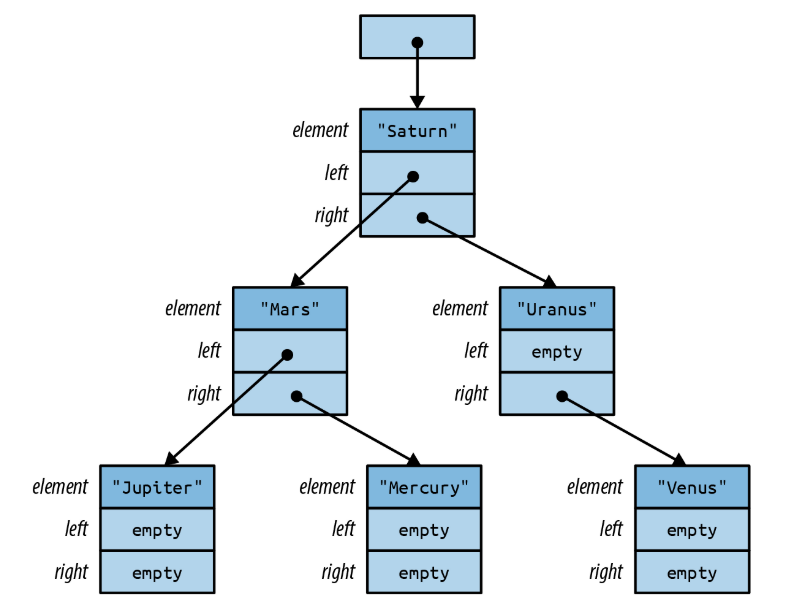
\includegraphics[width=0.9\textwidth]{../img/f10-3.png}
    \caption{一个包含6个字符串的\texttt{BinaryTree}}
    \label{f10-3}
\end{figure}

构建这棵树中的节点非常直观:
\begin{minted}{Rust}
    use self::BinaryTree::*;
    let jupiter_tree = NonEmpty(Box::new(TreeNode {
        element: "Jupiter",
        left: Empty,
        right: Empty,
    }));
\end{minted}

更大的树可以通过较小的树构建:
\begin{minted}{Rust}
    let mars_tree = NonEmpty(BOx::new(TreeNode {
        element: "Mars",
        left: jupiter_tree,
        right: mercury_tree,
    }));
\end{minted}

自然地,这个赋值会把\texttt{jupiter\_node}和\texttt{mercury\_node}的所有权移动到新的父节点里。

树的其他部分遵循相同的模式。根节点和其它节点不同:
\begin{minted}{Rust}
    let tree = NonEmpty(Box::new(TreeNode {
        element: "Saturn",
        left: mars_tree,
        right: uranus_tree,
    }));
\end{minted}

在这一章的后续部分中,我们将介绍怎么在\texttt{BinaryTree}类型上实现一个\texttt{add}方法,这样我们就可以这样写:
\begin{minted}{Rust}
    let mut tree = BinaryTree::Empty;
    for planet in planets {
        tree.add(planet);
    }
\end{minted}

无论你之前用什么语言,在Rust中创建像\texttt{BinaryTree}这样的数据结构都需要一些练习。一开始把\texttt{Box}放在哪可能并不明显。一种寻找设计的方法是画一幅像\hyperref[f10-3]{图10-3}这样的内存布局图。然后根据图设计代码:每一个矩形都是一个结构体或者元组,每一个箭头都是一个\texttt{Box}或者其他智能指针。搞清楚每个字段的类型有点困难,但解决难题的回报是控制程序的内存使用。 

现在就到了我们在本章开始时提到的“代价”。枚举的标签字段要占用很小的内存,最糟的情况下要占用8个字节,但这种情况通常非常少见。枚举真正的缺点(如果它能被称为缺点的话)是Rust不能忽略安全性、不管当前的值是什么直接尝试访问字段:
\begin{minted}{Rust}
    let r = shape.radius;   // 错误:`Shape`类型没有字段`radius`
\end{minted}

访问枚举中的值的唯一方式是:使用枚举,这是一种安全的方式。

\section{模式}

回顾一下我们在本章中定义过的\texttt{RoughTime}:
\begin{minted}{Rust}
    enum RoughTime {
        InThePast(TimeUnit, u32),
        JustNow,
        InTheFuture(TimeUnit, u32),
    }
\end{minted}

假设你有一个\texttt{RoughTime}值并且你想在网页中显示它。你需要访问值里的\texttt{TimeUnit}和\texttt{u32}字段。Rust不允许你直接通过\texttt{rough\_time.0}和\texttt{rough\_time.1}访问它们,因为毕竟此时值也可能是\texttt{RoughTime::JustNow},而它没有字段。那么,你怎么获取数据呢?

你需要一个\texttt{match}表达式:
\begin{minted}[linenos,numbersep=-1em]{Rust}
    fn rough_time_to_english(rt: RoughTime) -> String {
        match rt {
            RoughTime::InThePast(units, count) =>
                format!("{} {} ago", count, units.plural()),
            RoughTime::JustNow =>
                format!("just now"),
            RoughTime::InTheFuture(units, count) =>
                format!("{} {} from now", count, units.plural()),
        }
    }
\end{minted}
\texttt{match}会进行模式匹配。在这个例子中,\emph{模式}是第3、5、7行中出现在\texttt{=>}符号左边的部分。匹配\texttt{RoughTime}值的模式看起来就像是一个创建\texttt{RoughTime}值的表达式。这并不是巧合。表达式\emph{产生}值,模式\emph{消耗}值。它们使用相同的语法。

让我们逐步看看运行这个\emph{match}表达式时发生了什么。假设\texttt{rt}的值是\texttt{RoughTime::InTheFuture(TimeUnit::Months, 1)}。Rust首先尝试将这个值和第3行的模式匹配。正如\hyperref[f10-4]{图10-4}所示,它并不能匹配。

\begin{figure}[htbp]
    \centering
    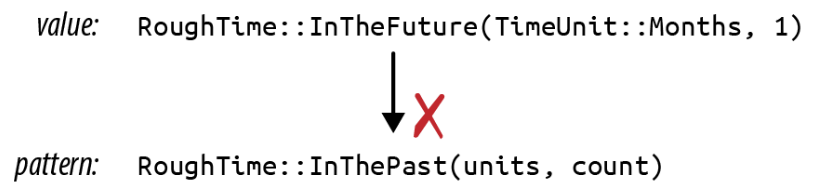
\includegraphics[width=0.8\textwidth]{../img/f10-4.png}
    \caption{一个\texttt{RoughTime}值和不匹配的模式}
    \label{f10-4}
\end{figure}

Rust中用于匹配一个枚举、结构体或者元组的模式的工作原理就好像简单地从左到右扫描,检查模式中的每个部分来看看是不是和值匹配。如果不是,Rust会移动到下一个模式。

第3和第5行的模式都匹配失败。但第7行的模式成功了(\hyperref[f10-5]{图10-5})。

\begin{figure}[htbp]
    \centering
    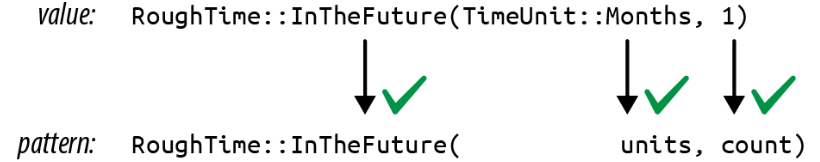
\includegraphics[width=0.8\textwidth]{../img/f10-5.png}
    \caption{一个成功的匹配}
    \label{f10-5}
\end{figure}

当一个模式包含像\texttt{units}和\texttt{count}这样的简单标识符时,在匹配之后的代码中它们会变为局部变量。当前值里的任何内容都会被拷贝或移动到新的变量中。Rust把\texttt{TimeUnit::Months}存储在\texttt{units}中,把\texttt{1}存储在\texttt{count}中,然后运行第8行的代码,最后返回字符串\texttt{"1 months from now"}。

这个输出有一点语法上的错误,可以通过给\texttt{match}添加另一个分支来修正:
\begin{minted}{Rust}
    RoughTime::InTheFuture(unit, 1) =>
        format!("a {} from now", unit.singular()),
\end{minted}

只有当\texttt{count}字段恰好是1时这个分支才能匹配。注意这一段新代码必须添加到第7行之前。如果我们把它添加在最后,那么执行流永远不会到达它,因为第7行匹配所有的\texttt{InTheFuture}值。如果你犯了这种错误,Rust编译器会给出一个“不可达的模式”警告。

即使有了新的代码,\texttt{RoughTime::InTheFuture(TimeUnit::Hours, 1)}仍然有一个问题:结果\texttt{"a hour from now"}在英语中并不是完全正确。这可以通过给\texttt{match}添加另一个分支来修复。

正如这个例子所示,模式匹配和枚举协同工作,甚至可以测试它们包含的值,这使得\texttt{match}表达式成为C的\texttt{switch}语句的一个更强大、更灵活的替代。

到目前为止,我们只见到了匹配枚举值的模式。其实它还有更多用途。Rust的模式有它们自己的语言,\hyperref[t10-1]{表10-1}中进行了总结。我们将用本章中剩下的大部分内容来展示表中的特性。

\begin{table}[htbp]
    \centering
    \caption{模式}
    \label{t10-1}
    \begin{tabular}{p{0.15\textwidth}p{0.35\textwidth}p{0.4\textwidth}}
        \hline
        \textbf{模式类型} & \textbf{示例} & \textbf{注释} \\
        \hline
        字面量  & \makecell[l]{\texttt{100} \\ \texttt{"name"}} & 匹配一个精确值,也可以使用一个\texttt{const}的值的名称    \\
        \rowcolor{tablecolor}
        范围    & \makecell[l]{\texttt{0 ..= 100} \\ \texttt{'a' ..= 'k'}}  & 匹配范围内的任何值,包括终点值 \\
        通配符  & \texttt{\_}   & 匹配任何值并忽略  \\
        \rowcolor{tablecolor}
        变量    & \makecell[l]{\texttt{name} \\ \texttt{mut count}} & 类似\texttt{\_}但是把值移动或拷贝进新的局部变量   \\
        \texttt{ref}变量    & \makecell[l]{\texttt{ref field} \\ \texttt{ref mut field}}    & 借用匹配的值的引用,而不是移动或拷贝它    \\
        \rowcolor{tablecolor}
        带子模式的绑定  & \makecell[l]{\texttt{val @ 0 ..= 99} \\ \texttt{ref circle @ Shape::Circle \{ .. \}}} & 匹配@右侧的模式,使用左侧作为变量名   \\
        枚举模式    & \makecell[l]{\texttt{Some(value)} \\ \texttt{None} \\ \texttt{Pet::Orca}} & \\
        \rowcolor{tablecolor}
        元组模式    & \makecell[l]{\texttt{(key, value)} \\ \texttt{(r, g, b)}} & \\
        数组模式    & \makecell[l]{\texttt{[a, b, c, d, e, f, g]} \\ \texttt{[heading, carom, correction]}} & \\
        \rowcolor{tablecolor}
        切片模式    & \makecell[l]{\texttt{[first, second]} \\ \texttt{[first, \_, third]} \\ \texttt{[first, .., nth]} \\ \texttt{[]}}  & \\
        结构体模式  & \makecell[l]{\texttt{Color(r, g, b)} \\ \texttt{Point \{ x, y \}} \\ \texttt{Card \{ suit: Clubs, rank: n \}} \\ \texttt{Account \{ id, name, .. \}}} & \\
        \rowcolor{tablecolor}
        引用    & \makecell[l]{\texttt{\&value} \\ \texttt{\&(k, v)}}   & 只匹配引用值 \\
        多重模式    & \texttt{'a' | 'A'}    & 只能用作可反驳的模式(\texttt{match, if let, while let}) \\
        \rowcolor{tablecolor}
        守卫表达式  & \texttt{x if x * x <= r2} & 只能在\texttt{match}中使用(在\texttt{let}等表达式中无效) \\
    \end{tabular}
\end{table}

\subsection{模式中的字面量、变量和通配符}
到目前为止,我们已经展示了\texttt{match}表达式和枚举一起使用,其实其它类型也可以用模式来匹配。当你需要类似C的\texttt{switch}语句的功能时,可以使用处理整数值的\texttt{match}表达式。整数字面量例如\texttt{0}和\texttt{1}可以用作模式:
\begin{minted}{Rust}
    match meadow.count_rabbits() {
        0 => {} // 什么都不输出
        1 => println!("A rabbit is nosing around in the clover."),
        n => println!("There are {} rabbits hopping about in the meadow", n),
    }
\end{minted}

当草地上没有兔子时模式\texttt{0}会匹配,当只有一只时\texttt{1}会匹配。如果有两只或者更多兔子,就会到达第三个模式\texttt{n}。这个模式只有一个变量名。它可以匹配任何值,被匹配的值会被移动或拷贝进新的局部变量。因此在这个例子中,\texttt{meadow.count\_rabbits()}的值被存储在一个新的局部变量\texttt{n}中,然后我们打印出它。

其他的字面量也可以用作模式,包括布尔值、字符、甚至字符串:
\begin{minted}{Rust}
    let calendar = match settings.get_string("calendar") {
        "gregorian" =>  Calendar::Gregorian,
        "chinese" => Calendar::Chinese,
        "ethiopian" => Calendar::Ethiopian,
        other => return parse_error("calendar", other),
    };
\end{minted}

在这个例子中,\texttt{other}和上个例子中的\texttt{n}一样用作匹配任何值的模式。这些模式和\texttt{switch}语句中的\texttt{default}标签一样,用来匹配其他所有模式都匹配不了的值。

如果你需要一个匹配所有值的模式,但又不关心匹配到的值,你可以使用单个下划线\texttt{\_}作为模式,也就是\emph{通配模式}:
\begin{minted}{Rust}
    let caption = match photo.tagged_pet() {
        Pet::Tyrannosaur => "RRRAAAAAHHHHHH",
        Pet::Samoyed => "*dog thoughts*",
        _ => "I'm cute, love me",   // 通用标题,用于任何宠物
    };
\end{minted}

通配模式匹配任何值,但并不存储它。因为Rust要求每一个\texttt{match}表达式要能处理所有可能的值,因此最后通常需要一个通配符。即使你非常确信其他的情况不会发生,你也必须至少添加一个fallback分支,这个分支里可以直接panic:
\begin{minted}{Rust}
    // 有很多形状,但我们只支持“选择”文本或者一个矩形区域。
    // 你不能选择一个椭圆或者梯形。
    match document.selection() {
        Shape::TextSpan(start, end) => paint_text_selection(start, end),
        Shape::Rectangle(rect) => paint_rect_selection(rect),
        _ => panic!("unexpected selection type"),
    }
\end{minted}

\subsection{元组和结构体模式}
元组模式匹配元组。当你想在单个\texttt{match}中获得数据的多个部分时它们会很有用:
\begin{minted}{Rust}
    fn describe_point(x: i32, y: i32) -> &'static str {
        use std::cmp::Ordering::*;
        match (x.cmp(&0), y.cmp(&0)) {
            (Equal, Equal) => "at the origin",
            (_, Equal) => "on the x axis",
            (Equal, _) => "on the y axis",
            (Greater, Greater) => "in the first quadrant",
            (Less, Greater) => "in the second quadrant",
            _ => "somewhere else",
        }
    }
\end{minted}

结构体模式要使用花括号,就和结构体表达式一样。它们可以包含每个字段的子模式:
\begin{minted}{Rust}
    match balloon.location {
        Point { x: 0, y: height } =>
            println!("straight up {} meters", height),
        Point { x: x, y: y } =>
            println!("at ({}m, {}m)", x, y),
    }
\end{minted}

在这个例子中,如果第一个分支匹配了,那么\texttt{balloon.location.y}会被存储到新的局部变量\texttt{height}。

假设\texttt{balloon.location}是\texttt{Point \{ x: 30, y: 40 \}}。和之前一样,Rust会按照\hyperref[f10-6]{图10-6}的顺序检查每一个模式的每一个部分。

\begin{figure}[htbp]
    \centering
    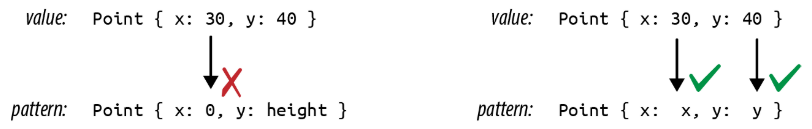
\includegraphics[width=0.8\textwidth]{../img/f10-6.png}
    \caption{结构体模式匹配}
    \label{f10-6}
\end{figure}

第二个分支可以匹配,因此输出将是\texttt{at (30m, 40m)}。

当匹配结构体时类似\texttt{Point \{ x: x, y: y \}}的模式非常常见,多余的名字也只会扰乱视觉,因此Rust为此支持一种缩写形式\texttt{Point \{x, y\}}。含义和之前相同,这个模式也会把点的\texttt{x}字段存储在新的局部变量\texttt{x}、把\texttt{y}字段存储在新的局部变量\texttt{y}。

即使有了缩写形式,如果我们要匹配一个很大的结构体但又只关心少数字段时还是会很麻烦:
\begin{minted}{Rust}
    match get_account(id) {
        ...
        Some(Account {
                name, language, // 我们关心的两个字段
                id: _, status: _, address: _, birthday: _, eye_color: _,
                pet: _, security_question: _, hashed_innermost_secret: _,
                is_adamantium_preferred_customer: _, }) =>
            language.show_custom_greeting(name),
    }
\end{minted}

为了避免这种情况,可以使用\texttt{..}告诉Rust你不关心其他的字段:
\begin{minted}{Rust}
    Some(Account { name, language, .. }) =>
        language.show_custom_greeting(name),
\end{minted}

\subsection{数字和切片模式}
数组模式匹配数组。它们被通常被用来过滤出某些特殊值,当数组的不同位置的含义不同时它们也会变得很有用。

例如,当把色相、饱和度、亮度(HSL)颜色值转换为红绿蓝(RGB)颜色值时,亮度为0的颜色就是黑、而亮度为满的颜色就是白。我们可以使用\texttt{match}表达式来简单地处理这些情况:
\begin{minted}{Rust}
    fn hsl_to_rgb(hsl: [u8; 3]) -> [u8; 3] {
        match hsl {
            [_, _, 0] => [0, 0, 0],
            [_, _, 255] => [255, 255, 255],
            ...
        }
    }
\end{minted}

切片模式与此类似,单核数组不同的是,切片的长度可以变化。因此切片模式并不只匹配值,还要匹配长度。切片模式中的\texttt{..}匹配任意数量的元素:
\begin{minted}{Rust}
    fn greet_people(names: &[&str]) {
        match names {
            [] => { println!("Hello, nobody.") },
            [a] => { println!("Hello, {}.", a) },
            [a, b] => { println!("Hello, {} and {}.", a, b) },
            [a, .., b] => { println!("Hello, everyone from {} to {}.", a, b) }
        }
    }
\end{minted}

\subsection{引用模式}
Rust模式支持两种和引用有关的特性。\texttt{ref}模式会借用被匹配的值,\texttt{\&}模式匹配引用。我们将首先介绍\texttt{ref}模式。

匹配一个非拷贝类型的值会移动这个值。继续上面的例子,下面的代码是无效的:
\begin{minted}{Rust}
    match account {
        Account { name, language, .. } => {
            ui.greet(&name, &language);
            ui.show_settings(&account); // error: borrow of moved value: `account`
        }
    }
\end{minted}

这里,字段\texttt{account.name}和\texttt{account.language}被移动进局部变量\texttt{name}和\texttt{language}中。\texttt{account}的其他部分被丢弃。这就是为什么我们不能再借用它的引用。

如果\texttt{name}和\texttt{language}都是可拷贝的值,Rust将会拷贝字段而不是移动它们,代码将没有问题。但假设它们就是\texttt{String},那我们该怎么办?

我们需要一种模式\emph{借用}被匹配的值而不是移动它们。\texttt{ref}关键字就是为此而生:
\begin{minted}{Rust}
    match account {
        Account { ref name, ref language, .. } => {
            ui.greet(name, language);
            ui.show_settings(&account); // ok
        }
    }
\end{minted}

现在局部变量\texttt{name}和\texttt{language}都是\texttt{account}中相应字段的引用。因此\texttt{account}只是被借用,并没有被消耗,所以继续用它调用方法也是OK的。

你可以使用\texttt{ref mut}来借用\texttt{mut}引用:
\begin{minted}{Rust}
    match line_result {
        Err(ref err) => log_error(err), // `err`是&Error(shared ref)
        Ok(ref mut line) => {           // `line`是&mut String(mut ref)
            trim_comments(line);        // 修改String
            handle(line);
        }
    }
\end{minted}

模式\texttt{Ok(ref mut line)}匹配任何成功值,并借用存储在里面的成功值的\texttt{mut}引用。

另一种相反的引用模式是\texttt{\&}模式。一个以\texttt{\&}开始的模式只能匹配引用:
\begin{minted}{Rust}
    match sphere.center() {
        &Point3d { x, y, z } => ...
    }
\end{minted}

在这个例子中,假设\texttt{sphere.center()}返回一个\texttt{sphere}的私有字段的引用,这在Rust中是很常见的。返回的值是一个\texttt{Point3d}的引用。如果中心在原点的话,\texttt{sphere.center()}会返回\texttt{\&Point3d \{ x: 0.0, y: 0.0, z: 0.0 \}}。

模式匹配按照\hyperref[f10-7]{图10-7}进行。

\begin{figure}[htbp]
    \centering
    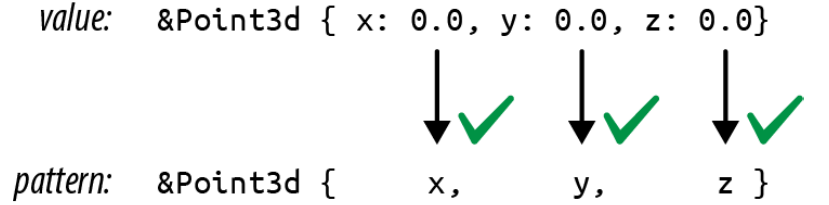
\includegraphics[width=0.8\textwidth]{../img/f10-7.png}
    \caption{引用的模式匹配}
    \label{f10-7}
\end{figure}

这里有一点诡异,因为Rust在这里解除了引用,也就是\texttt{*}运算符的功能。要住的是模式和表达式天然是相反的。表达式\texttt{(x, y)}把两个值放入一个新的元组中,而模式\texttt((x, y))恰好相反:它匹配一个元组然后取出两个值。\texttt{\&}也是一样,在表达式里,\texttt{\&}创建一个引用;在模式里,\texttt{\&}匹配一个引用。

匹配一个引用遵循我们期望的所有规则。生命周期是强制的。你不能通过共享引用获取\texttt{mut}访问权限。你不能将值移动出引用,即使是\texttt{mut}引用。当我们匹配\texttt{\&Point3d \{ x, y, z \}}时,变量\texttt{x, y, z}都是坐标的拷贝,原本的\texttt{Point3d}值还是完整的。只有当这些字段都是拷贝类型才可以正常工作。如果我们想对结构体中一个不可拷贝的字段这么做,我们会遇到错误:
\begin{minted}{Rust}
    match friend.borrow_car() {
        Some(&Car { engine, .. }) => // error: can't move out of borrow
            ...
        None => {}
    }
\end{minted}

把一辆借来的车报废是不好的,Rust也不会允许这么做。你可以使用\texttt{ref}模式来借用一个引用,这样就不用拥有它:
\begin{minted}{Rust}
    Some(&Car { ref engine, .. }) => // ok, engine is a reference
\end{minted}

再来看另一个\texttt{\&}模式的例子。假设我们有一个迭代器\texttt{chars}迭代一个字符串里的所有字符,并且它有一个方法\texttt{chars.peek()}返回一个\texttt{Option<\&char>}:一个指向下一个字符的引用,如果有的话。(这类迭代器确实返回一个\texttt{Option<\&ItemType>},我们将在\hyperref[ch15]{第15章}中见到。)

一个程序可以使用\texttt{\&}来获得指向的字符:
\begin{minted}{Rust}
    match chars.peek() {
        Some(&c) => println!("coming up: {:?}", c),
        None => println!("end of chars"),
    }
\end{minted}

\subsection{匹配守卫}
有时一个匹配分支还有附加的条件必须要满足。假设我们在实现一个六边形空间内的棋子游戏,玩家只需要点击即可移动棋子。为了确认点击时有效的,我们可能要尝试类似这样的代码:
\begin{minted}{Rust}
    fn check_move(current_hex: Hex, click: Point) -> game::Result<Hex> {
        match point_to_hex(click) {
            None =>
                Err("That's not a game space."),
            Some(current_hex) => // 尝试匹配用户是不是点击了当前位置
                                 // (这样是错误的:原因如下)
                Err("You are already there! You must click somewhere else."),
            Some(other_hex) =>
                Ok(other_hex)
        }
    }
\end{minted}

这样是错误的,因为模式里的标识符会引入\emph{新的}变量。模式\texttt{Some(current\_hex)}会创建一个新的叫\texttt{current\_hex}的局部变量,然后遮蔽参数\texttt{current\_hex}。Rust会为这段代码报出好几个警告——尤其是,最后一个\texttt{match}分支不可达。一种修复这个问题的方法是简单地在分支中使用一个\texttt{if}表达式:
\begin{minted}{Rust}
    match point_to_hex(click) {
        None => Err("That's not a game space."),
        Some(hex) => {
            if hex == current_hex {
                Err("You are already there! You must click somewhere else")
            } else {
                Ok(hex)
            }
        }
    }
\end{minted}

不过Rust还提供了\emph{匹配守卫(match guard)}:模式和分支的\texttt{=>}词元中间的\texttt{if CONDITION}条件必须满足才能匹配:
\begin{minted}{Rust}
    match point_to_hex(click) {
        None => Err("That's not a game space."),
        Some(hex) if hex == current_hex =>
            Err("You are already there! You must click somewhere else"),
        Some(hex) => Ok(hex)
    }
\end{minted}

如果模式匹配,但条件不满足,那么将会继续匹配下一个分支。

\subsection{匹配多种可能}
竖线(|)可以用于在一个\texttt{match}分支中组合多个模式:
\begin{minted}{Rust}
    let at_end = match chars.peek() {
        Some(&'\r') | Some(&'\n') | None => true,
        _ => false,
    };
\end{minted}

在一个表达式中,|是位或运算符,但这里它的功能就像是普通表达式中的\texttt{||}。如果\texttt{chars.peek()}能匹配三个模式中的任意一个,\texttt{at\_end}就会被设为\texttt{true}。

使用\texttt{..=}来匹配范围内的值。范围模式包括起点和终点值,因此\texttt{'0' ..= '9'}匹配所有的ASCII数字:
\begin{minted}{Rust}
    match next_char {
        '0'..='9' => self.read_number(),
        'a'..='z' | 'A'..='Z' => self.read_word(),
        ' ' | '\t' | '\n' => self.skip_whitespace(),
        _ => self.handle_punctuation(),
    }
\end{minted}

Rust(目前)不允许在模式中使用尾开区间例如\texttt{0..100}。

\subsection{绑定和\texttt{@}模式}




    \chapter{trait与泛型}\label{ch11}

\emph{[A] computer scientist tends to be able to deal with nonuniform structures—case 1, case 2, case 3—while a mathematician will tend to want one unifying axiom that governs an entire system.}

\begin{flushright}
    ——Donald Knuth
\end{flushright}

编程界中最伟大的发现之一就是可以编写处理多种不同类型的代码,\emph{即使是还没有定义出来的类型也可以}。这里有两个例子:
\begin{itemize}
    \item \texttt{Vec<T>}是泛型的:你可以创建一个任意类型的vector,包括你自己定义的类型,即使\texttt{Vec}的作者完全不知道这个类型。
    \item 很多类型都有\texttt{.write()}方法,包括\texttt{File}和\texttt{TcpStream}。你的代码可以通过引用获取一个writer(任意的writer),并向它写入数据。你的代码不需要关心那个writer到底是什么类型。然后,如果有人添加了一个新的writer类型,你的代码将会自动支持它。
\end{itemize}

当然,这并不是什么新鲜的功能。它被称为\emph{多态(polymorphism)},是20世纪70年代很热门的新的编程语言技术。但现在它已经非常普遍了。Rust使用两个相关的特性来支持多态:trait和泛型。很多程序员可能已经很熟悉这两个概念了,但Rust采用了一种受Haskell的typeclass启发的新方法。

\emph{trait}是Rust中的接口或抽象基类。首先,它们看起来很像Java或C\#中的接口。用于写入字节的trait叫做\texttt{std::io::Write},它在标准库中的定义看起来像这样:
\begin{minted}{Rust}
    trait Write {
        fn write(&mut self, buf: &[u8]) -> Result<usize>;
        fn flush(&mut self) -> Result<()>;

        fn write_all(&mut self, buf: &[u8]) -> Result<()> { ... }
        ...
    }
\end{minted}

这个trait提供了几个方法,我们只展示了前三个。

标准类型\texttt{File}和\texttt{TcpStream}都实现了\texttt{std::io::Write}。\texttt{Vec<u8>}也是。这三个类型都提供\texttt{.write()}、\texttt{.flush()}等方法。使用writer的代码不需要关心它的类型,像这样:
\begin{minted}{Rust}
    use std::io::Write;

    fn say_hello(out: &mut dyn Write) -> std::io::Result<()> {
        out.write_all(b"hello world\n")?;
        out.flush()
    }
\end{minted}

\texttt{out}的类型是\texttt{\&mut dyn Write},意思是“任何实现了\texttt{Write} trait的值的可变引用”。我们可以把任何这样的值的可变引用传递给\texttt{say\_hello}:
\begin{minted}{Rust}
    use std::fs::File;
    let mut local_file = File::create("hello.txt")?;
    say_hello(&mut local_file)?;    // 可以工作

    let mut bytes = vec![];
    say_hello(&mut bytes)?;         // 也可以工作
    assert_eq!(bytes, b"hello world\n");
\end{minted}

这一章首先展示trait怎么使用、怎么工作、怎么定义自己的trait。但trait的用途比我们目前提到的更多。我们将使用它们给现有类型添加扩展的方法,甚至像\texttt{str}和\texttt{bool}这种内建类型也可以。我们将会解释为什么给一个类型添加trait不会消耗多余的内存,以及如何在没有虚方法开销的情况下使用trait。我们将看到一些Rust提供的用于操作符重载和其他特性的语言内建的trait。我们还将介绍\texttt{Self}类型、关联函数、关联类型。Rust从Haskell中提取了这三个特性,它们可以优雅地解决其他语言中需要通过变通的方法或者hack才能解决的问题。 

\emph{泛型}是Rust中另一种形式的多态。类似于C++的模板,一个泛型函数或类型可以用于多种不同的类型:
\begin{minted}{Rust}
    /// 给定两个值,找出较小的那个
    fn min<T: Ord>(value1: T, value2: T) -> T {
        if value1 <= value2 {
            value1
        } else {
            value2
        }
    }
\end{minted}

这个函数中的\texttt{<T: Ord>}意味着\texttt{min}可以用于任何实现了\texttt{Ord} trait的类型\texttt{T}——也就是,任何有序的类型。这样的一个要求被称为\emph{约束(bound)},因为它列举出了类型\texttt{T}需要满足的限制。编译器会为你实际使用的每一个类型\texttt{T}生成自定义的机器代码。

泛型和trait紧密相关:泛型函数在约束中使用trait来表明它可以用于哪些类型的参数。所以我们还会讨论\texttt{\&mut dyn Write}和\texttt{<T: Write>}有哪些相似和不同之处,以及如何在这种两种使用trait的方式中选择。

\section{使用trait}

一个trait就是一个给定的类型可能支持也可能不支持的特性。通常,一个trait代表一种能力:一个类型可以做的事情。
\begin{itemize}
    \item 一个实现了\texttt{std::io::Write}的值可以写入字节。
    \item 一个实现了\texttt{std::iter::Iterator}的值可以产生值的序列。
    \item 一个实现了\texttt{std::clone::Clone}的值可以产生自身在内存中的克隆。
    \item 一个实现了\texttt{std::fmt::Debug}可以使用\texttt{println!()}的\texttt{\{:?\}}格式说明符进行打印。
\end{itemize}

那4个trait都是Rust标准库的一部分,有很多标准类型都实现了它们。例如:
\begin{itemize}
    \item \texttt{std::fs::File}实现了\texttt{Write} trait,它把字节写入到本地文件。\texttt{std::net::TcpStream}写入到网络连接。\texttt{Vec<u8>}也实现了\texttt{Write}。在字节vector上调用\texttt{.write()}会往尾部添加数据。
    \item \texttt{Range<i32>}(\texttt{0..10}的类型)实现了\texttt{Iterator} trait,一些和切片、哈希表等相关联的迭代器类型也实现了这个trait。
    \item 大多数标准库类型实现了\texttt{Clone}。一些例外主要是像\texttt{TcpStream}这样的不仅仅表示内存中的数据的类型。
    \item 大多数标准库类型支持\texttt{Debug}。
\end{itemize}

有关trait方法有一个不寻常的规则:trait自身必须在作用域里。否则,所有它的方法都会被隐藏:
\begin{minted}{Rust}
    let mut buf: Vec<u8> = vec![];
    buf.write_all(b"hello")?;   // 错误:没有叫`write_all`的方法
\end{minted}

这种情况下,编译器会打印出友好的错误消息建议你添加\texttt{std::io::Write},然后确实能修复这个问题:
\begin{minted}{Rust}
    use std::io::Write;

    let mut buf: Vec<u8> = vec![];
    buf.write_all(b"hello")?;   // ok
\end{minted}

Rust会有这个规则是因为,正如我们稍后会在本章中看到的,你可以使用trait来给任意类型添加新的方法——即使是标准库的类型例如\texttt{u32}和\texttt{str}。第三方的crate也可以做同样的事情。显然,这会导致名称冲突!但因为Rust让你自己导入你需要使用的trait,所以crate可以轻松地利用这种强大的功能。要想导致冲突,你需要导入两个trait,这两个trait要给同一个类型添加相同名称的方法。这在实践中是很少见的。(如果你确实陷入了冲突中,你可以使用本章稍后会介绍的\nameref{fullymethod}来指明你想要使用哪一个。)

\texttt{Clone}和\texttt{Iterator}的方法不需要特殊的导入是因为它们默认总是在作用域里,它们是标准prelude的一部分:Rust会自动导入每个模块中的名称。事实上,prelude就是一个精心挑选的trait的集合。我们将在\hyperref[ch13]{第13章}中介绍更多有关它们的内容。

C++和C\#程序员可能已经注意到了trait方法很像虚方法。然而,类似上面的函数调用速度很快,与任何其他方法调用一样快。简单来说,这里面并没有多态性。显然\texttt{buf}是一个vector,不是一个文件或者网络连接,所以编译器可以简单地生成一个\texttt{Vec<u8>::write()}的调用。它甚至可以内联这个方法。(C++和C\#通常也会这样,尽管子类化的可能性有时会排除这一点。)只有通过\texttt{\&mut dyn Write}的调用才会有动态分发的开销,这种调用也被称为虚方法调用,类型里的\texttt{dyn}关键字暗示了这一点。\texttt{dyn Write}被称为\emph{trait对象(trait object)};我们将会在接下来的小节中看到trait对象的技术细节,以及它们与泛型函数的比较。

\subsection{trait对象}\label{traitobject}
在Rust中有两种使用trait来编写多态代码的方式:trait对象和泛型。我们将会首先介绍trait对象,在下一节中介绍泛型。

Rust不允许\texttt{dyn Write}类型的变量:
\begin{minted}{Rust}
    use std::io::Write;

    let mut buf: Vec<u8> = vec![];
    let writer: dyn Write = buf; // 错误:`Write`并没有固定的大小
\end{minted}

一个变量的大小必须在编译期时已知,然而实现了\texttt{Write}的类型可以是任何大小。

如果你来自C\#或者Java的话可能会感觉很惊讶,但原因其实很简单。在Java中,一个\texttt{OutputStream}(Java中类似\texttt{std::io::Write}的标准接口)类型的变量是一个任何实现了\texttt{OutputStream}的对象的引用。它是一个引用的事实不言而喻,C\#以及其他大多数语言中的接口也是一样。

我们在Rust中想要的也是一样的,但是在Rust中引用是显式的:
\begin{minted}{Rust}
    let mut buf: Vec<u8> = vec![];
    let writer: &mut dyn Write = &mut buf;  // ok
\end{minted}

一个trait类型的引用,例如\texttt{writer},被称为一个\emph{trait对象}。和其他引用一样,一个trait对象指向某个值、它有生命周期、它可以是可变的或者是共享的。

让一个trait对象与众不同的是Rust在编译期通常不知道被引用值的类型是什么。因此一个trait对象包括一点额外的有关被引用值的类型信息。类型信息被严格限制为只有Rust自己可以在幕后使用:当你调用\texttt{writer.write(data)}时,Rust需要这个类型信息来依据\texttt{*writer}的类型动态调用正确的\texttt{write}方法。你不能直接查询类型信息,Rust也不支持将trait对象\texttt{\&mut dyn Write}向下转换回精确的类型例如\texttt{Vec<u8>}。

\subsubsection{trait对象的布局}
在内存中,一个trait对象是一个胖指针,由指向值的指针加上一个指向表示该值类型的表的指针组成。因此每一个trait对象要占两个机器字,如\hyperref[f11-1]{图11-1}所示。

\begin{figure}[htbp]
    \centering
    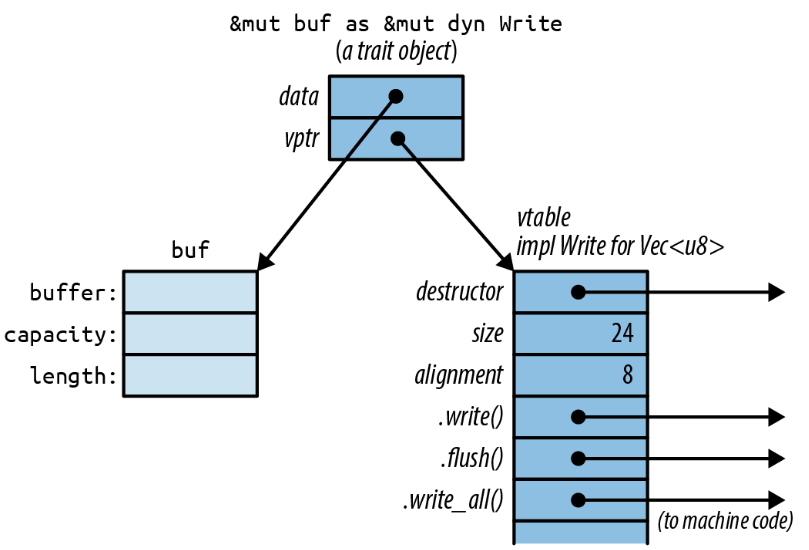
\includegraphics[width=0.9\textwidth]{../img/f11-1.png}
    \caption{内存中的trait对象}
    \label{f11-1}
\end{figure}

C++也有这种运行时的类型信息。它被称为\emph{虚表}或者\emph{vtable}。在Rust中和在C++中一样,vtable只会在编译期生成一次,然后被所有相同类型的对象共享。\hyperref[f11-1]{图11-1}中较深颜色的阴影显示的内容,包括vtable,都是Rust的私有实现。这些字段和数据结构你不能直接访问。当你调用trait对象的方法时语言本身会自动使用vtable来决定要调用哪个实现。

熟练的C++程序员可能会注意到Rust和C++采取的内存策略有些不同。在C++中,虚表指针或者称为\emph{vptr}被存储为结构体的一部分,而Rust使用胖指针来代替。结构体本身不包含任何自身字段之外的东西。这样,一个结构体可以实现一大堆trait而不需要包含一大堆vptr。即使像\texttt{i32}这样的大小还不足以容纳一个vptr的类型,也可以实现trait。

当需要时Rust会自动把普通引用转换为trait对象。这就是为什么我们能在这个例子中直接把\texttt{\&mut local\_file}传递给\texttt{say\_hello}:
\begin{minted}{Rust}
    let mut local_file = File::create("hello.txt")?;
    say_hello(&mut local_file)?;
\end{minted}

\texttt{\&mut local\_file}的类型是\texttt{\&mut File},而\texttt{say\_hello}的参数类型是\texttt{\&mut dyn Write}。因为\texttt{File}是一种writer,所以Rust允许这种普通引用到trait对象的转换。

同样的,Rust也乐于把\texttt{Box<File>}转换成\texttt{Box<dyn Write>},它拥有一个在堆上的writer:
\begin{minted}{Rust}
    let w: Box<dyn Write> = Box::new(local_file);
\end{minted}

\texttt{Box<dyn Write>}类似于\texttt{\&mut dyn Write},是一个胖指针:它包含writer自身的地址和vtable的地址。其他指针类型例如\texttt{Rc<dyn Write>}也一样。

这种转换是唯一创建trait对象的方法。编译器做的工作其实很简单,当转换发生时,Rust知道被引用值的真正类型(这个例子中是\texttt{File}),因此它只是加上了正确的vtable的地址、把普通指针变成了胖指针。

\subsection{泛型函数和类型参数}
在这一章的开始处,我们展示了\texttt{say\_hello()}函数,它以trait对象为参数。让我们把这个函数重新为泛型函数:
\begin{minted}{Rust}
    fn say_hello<W: Write>(out: &mut W) -> std::io::Result<()> {
        out.write_all(b"hello world\n")?;
        out.flush()
    }
\end{minted}

只有类型签名改变了:
\begin{minted}{Rust}
    fn say_hello(out: &mut dyn Write)   // 普通函数

    fn say_hello<W: Write>(out: &mut W) // 泛型函数
\end{minted}

让函数变为泛型函数的正是\texttt{<W: Write>}短语,它是一个\emph{类型参数}。它意味着在整个函数体内,\texttt{W}代表任何实现了\texttt{Write} trait的类型。按照习惯,类型参数通常是大写字母。

类型\texttt{W}到底是什么取决于泛型函数如何被调用:
\begin{minted}{Rust}
    say_hello(&mut local_file)?;    // 调用say_hello::<File>
    say_hello(&mut bytes)?;         // 调用say_hello<Vec<u8>>
\end{minted}

当你把\texttt{\&mut local\_file}传递给泛型的\texttt{say\_hello()}函数时,你实际是在调用\texttt{say\_hello::<File>()}。Rust会为这个函数生成机器码,机器码里还会调用\texttt{File::write\_all()}和\texttt{File::flush()}。当你传递\texttt{\&mut bytes}时,你实际是在调用\texttt{say\_hello::<Vec<u8>>()}。Rust会为这个版本的函数生成单独的机器码,然后调用相应的\texttt{Vec<u8>}的方法。在这两种情况下,Rust都从参数的类型推导出类型\texttt{W},这个过程被称为\emph{单态化(monomorphization)},编译器会自动进行处理。

你也可以指明类型参数:
\begin{minted}{Rust}
    say_hello::<File>(&mut local_file)?;
\end{minted}

很少情况下才需要显式写出参数,因为Rust通常可以通过参数推断出类型参数。这里,\texttt{say\_hello}泛型函数期望一个\texttt{\&mut W}参数,而我们传入了一个\texttt{\&mut File},因此Rust推断出\texttt{W = File}。

如果你正在调用的泛型函数并没有足以推断出参数的线索,你需要显式地指明:
\begin{minted}{Rust}
    // 调用一个没有参数的泛型方法collect<C>()
    let v1 = (0 .. 1000).collect();     // 错误:不能推断出类型
    let v2 = (0 .. 1000).collect::<Vec<i32>>(); // ok
\end{minted}

有时我们需要一个类型参数可以支持多种功能。例如,如果我们想打印出一个vector中出现次数最多的10个值,我们需要这些值可以打印:
\begin{minted}{Rust}
    use std::fmt::Debug;

    fn top_ten<T: Debug>(values: &Vec<T>) { ... }
\end{minted}

但这还不够。我们怎么判断哪个值是出现次数最多的?通常的办法是把每个值当作键存入一个哈希表。这意味着这些值需要支持\texttt{Hash}和\texttt{Eq}操作。\texttt{T}的约束还必须包括\texttt{Debug}。这种情况下应该使用的语法是\texttt{+}号:
\begin{minted}{Rust}
    use std::hash::Hash;
    use std::fmt::Debug;

    fn top_ten<T: Debug + Hash + Eq>(values: &Vec<T>) { ... }
\end{minted}

一些类型实现了\texttt{Debug}、一些实现了\texttt{Hash}、一些支持\texttt{Eq},还有少数类型例如\texttt{u32}和\texttt{String},实现了这三个trait,如\hyperref[f11-2]{图11-2}所示。

\begin{figure}[htbp]
    \centering
    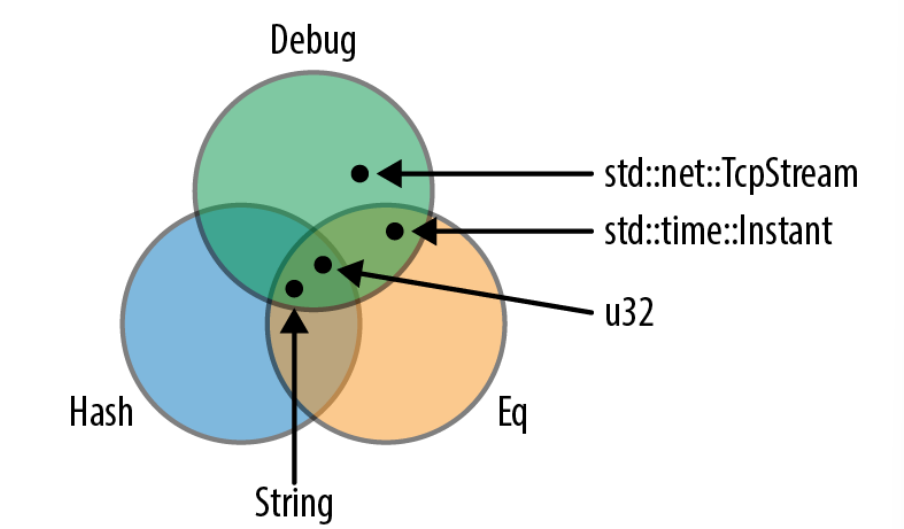
\includegraphics[width=0.8\textwidth]{../img/f11-2.png}
    \caption{trait作为类型的集合}
    \label{f11-2}
\end{figure}

也可以不给类型参数指定任何约束,但这样的话你几乎不能对它进行任何操作。你只能移动它、将它放在box或vector里。

泛型函数可以有多个类型参数:
\begin{minted}{Rust}
    /// 在一个大规模的分区数据集上进行查询。
    /// 见<http://research.google.com/archive/mapreduce.html>。
    fn run_query<M: Mapper + Serialize, R: Reducer + Serialize>(
        data: &DataSet, map: M, reduce: R) -> Results
    { ... }
\end{minted}

正如这个例子展示的一样,约束可能太长以至于很难阅读。Rust提供了使用关键字\texttt{where}的替代语法:
\begin{minted}{Rust}
    fn run_query<M, R>(data: &DataSet, map: M, reduce: R) -> Results
        where M: Mapper + Serialize,
              R: Reducer + Serialize
    { ... }
\end{minted}

类型参数\texttt{M}和\texttt{R}仍然在前边声明,但约束被移动到单独的行。这种\texttt{where}语法可以用于泛型结构体、泛型枚举、类型别名以及方法——任何允许约束的地方。

当然,\texttt{where}语法的一个替代是保持简单:寻找一种不需要大量使用泛型的方法来编写程序。

“\nameref{RefAsArg}”介绍了生命周期的语法。一个泛型函数可以同时有生命周期参数和类型参数。生命周期参数在前:
\begin{minted}{Rust}
    /// 返回`candidates`中距离`target`最近的点的引用。
    fn nearest<'t, 'c, P>(target: &'t P, candidates: &'c [P]) -> &'c P
        where P: MeasureDistance
    {
        ...
    }
\end{minted}

这个函数有两个参数:\texttt{target}和\texttt{candidates}。它们都是引用,但我们给了它们不同的生命周期\texttt{'t}和\texttt{'c}(正如在“\nameref{DistLife}”中讨论的那样)。这个函数可以用于任何实现了\texttt{MeasureDistance} trait的类型\texttt{P},因此我们可以在一个程序中用\texttt{Point2d}值调用它,而在另一个程序中用\texttt{Point3d}值调用它。

生命周期绝不会影响到机器码。两个\texttt{P}的类型相同但生命周期不同的\texttt{nearest()}的调用,将会调用同一个编译好的函数。只有不同的类型才会导致Rust编译一个泛型函数的多个拷贝。

当然,函数并不是Rust中唯一的泛型代码:
\begin{itemize}
    \item 我们已经在“\nameref{GenStruct}”和“\nameref{GenEnum}”中介绍过泛型类型了。
    \item 一个单独的方法也可以是泛型的,就算定义它的类型不是泛型的:
    \begin{minted}{Rust}
    impl PancakeStack {
        fn push<T: Topping>(&mut self, goop: T) -> PancakeResult<()> {
            goop.pour(&self);
            self.absorb_topping(goop)
        }
    }
    \end{minted}
    \item 类型别名也可以是泛型的:
    \begin{minted}{Rust}
    type PancakeResult<T> = Result<T, PancakeError>;
    \end{minted}
    \item 我们将在本章稍后介绍泛型trait。
\end{itemize}

所有这一节中介绍的特性——约束、\texttt{where}子句、生命周期参数等——可以被用于所有泛型item,而不仅仅是函数。

\subsection{选择哪一种}
选择trait对象还是泛型代码是一件很微妙的事情。因为它们都基于trait,有很多相似之处。

任何当你需要一个混合类型的值的集合的情况下trait对象都是正确的选择。从技术上讲创建泛型的沙拉是可行的:
\begin{minted}{Rust}
    trait Vegetable {
        ...
    }

    struct Salad<V: Vegetable> {
        veggies: Vec<V>
    }
\end{minted}

然而,这是一个非常糟糕的设计。每一个这样的沙拉都全部是由单一类型的蔬菜组成的。不是所有人都适合这么做,这本书的作者曾经为一个\texttt{Salad<IcebergLettuce}支付了\$14美元,并且直到现在也没有完全克服那次经历。

然而我们怎么构建一个更好的沙拉呢?因为\texttt{Vegetable}值可能是不同大小的,我们不能要求Rust创建一个\texttt{Vec<dyn Vegetable>}:
\begin{minted}{Rust}
    struct Salad {
        veggies: Vec<dyn Vegetable> // 错误:`dyn Vegetable`并
                                    // 没有固定大小
    }
\end{minted}

trait对象就是解决方案:
\begin{minted}{Rust}
    struct Salad {
        veggies: Vec<Box<dyn Vegetable>>
    }
\end{minted}

每一个\texttt{Box<dyn Vegetable>}可以持有任何类型的蔬菜,但box自身的大小是固定的——两个指针——因此可以存储在vector中。除了在食物里放盒子这个不幸的比喻之外,它确实就是我们需要的。它也同样适用于绘图应用中的形状、游戏中的怪物、网络路由器中的可插拔路由算法等等。

另一个使用trait对象的可能的原因是减小编译出的代码的体积。Rust可能需要编译一个泛型函数很多次,因为它要为每一个用到的类型都编译一次。这可能导致生成的二进制文件很大,这种现象在C++圈子里称为\emph{代码膨胀(code bloat)}。近年来内存越来越充裕,因此我们中的大多数人可以忽略代码的体积,但确实还有一些受限制的环境。

除了涉及到沙拉或者资源受限的环境之外,泛型与trait对象相比有三个优势。因此在Rust中泛型是更加普遍的选择。

第一个优势是速度。注意泛型函数签名中没有\texttt{dyn}关键字。因为你在编译期指明了确切的类型,不管是显式还是通过类型推导,编译器都知道实际上调用了哪个\texttt{write}。没有使用\texttt{dyn}关键字是因为没有trait对象——因此也没有涉及动态分发。

引言中展示的泛型\texttt{min()}函数就和我们单独编写\texttt{min\_u8}、\texttt{min\_i64}、\texttt{min\_string}等函数一样快。编译器还可以像其他函数一样内联它,因此在release构建中,一个对\texttt{min::<i32>}的调用可能只有两三条指令。对于常量的调用,例如\texttt{min(5, 3)}可能会更快:Rust可以在编译期对它进行求值,因此不会有任何运行时开销。

或者考虑这个泛型函数调用:
\begin{minted}{Rust}
    let mut sink = std::io::sink();
    say_hello(&mut sink);
\end{minted}

\texttt{std::io::sink()}返回一个\texttt{Sink}类型的writer,它会偷偷丢弃掉所有写入的字节。

当Rust为此生成机器码的时候,它可以产生先调用\texttt{Sink::write\_all}、再检查错误、最后调用\texttt{Sink::flush}的代码。这正是泛型函数体的内容。

或者,Rust可以查看那些方法,然后意识到下列情况:
\begin{itemize}
    \item \texttt{Sink::write\_all()}什么也不做。
    \item \texttt{Sink:flush()}什么也不做。
    \item 两个方法都不可能返回错误。
\end{itemize}

简单来说,Rust拥有所有优化掉这个函数调用所需的信息。

相比与trait对象的行为,Rust直到运行时才能知道一个trait对象指向的值到底是什么类型。因此即使你传递了一个\texttt{Sink},虚方法的调用开销和检查错误的开销仍然不可避免。

泛型的第二个优势是有的trait不支持trait对象。trait只支持一部分特性,例如关联函数只能使用泛型,这样就完全排除了trait对象。当我们将到这些特性时会指出它们。

泛型的第三个优势是可以很容易地一次给泛型类型参数添加多个trait约束,例如我们的\texttt{top\_ten}函数就要求它的参数\texttt{T}要实现\texttt{Debug + Hash + Eq}。trait对象不能这么做:Rust不支持类似\texttt{\&mut (dyn Debug + Hash + Eq)}这样的类型。(你可以用本章中稍后会讲到的\hyperref[subtrait]{子trait}来实现类似的功能,但这样有点复杂。)

\section{定义和实现trait}

定义一个trait很简单,只需要给出名字和trait方法的签名类型。假设我们在编写一个游戏,我们可能会定义像这样的trait:
\begin{minted}{Rust}
    /// 一个角色、物品、风景等
    /// 任何可以显示在屏幕上的游戏世界的物体。
    trait Visible {
        /// 在给定的画布上渲染这个对象。
        fn draw(&self, canvas: &mut Canvas);

        /// 如果点击(x, y)会选中这个对象就返回true。
        fn hit_test(&self, x: i32, y: i32) -> bool;
    }
\end{minted}

为了实现一个trait,需要使用语法\texttt{impl TraitName for Type}:
\begin{minted}{Rust}
    impl Visible for Broom {
        fn draw(&self, canvas: &mut Canvas) {
            for y in self.y - self.height -1 .. self.y {
                canvas.write_at(self.x, y, '|');
            }
            canvas.write_at(self.x, self.y , 'M);
        }

        fn hit_test(&self, x: i32, y: i32) -> bool {
            self.x == x
            && self.y - self.height - 1 <= y
            && y <= self.y
        }
    }
\end{minted}

注意\texttt{impl}包含了一份\texttt{Visible} trait中每个方法的实现,除此之外没有别的内容。在trait \texttt{impl}中定义的任何东西都必须是trait的特性。如果我们想要添加一个\texttt{Broom::draw()}的帮助函数,我们必须在单独的\texttt{impl}块中定义它:

\begin{minted}{Rust}
    impl Broom {
        /// 下面的Broom::draw()用到的帮助函数。
        fn broomstick_range(&self) -> Range<i32> {
            self.y - self.height - 1 .. self.y
        }
    }
\end{minted}

这些帮助函数可以在trait \texttt{impl}块中使用:
\begin{minted}{Rust}
    impl Visible for Broom {
        fn draw(&self, canvas: &mut Canvas) {
            for y in self.broomstick_range() {
                ...
            }
            ...
        }
        ...
    }
\end{minted}

\subsection{默认方法}
我们之前讨论的\texttt{Sink} writer可以用少数几行代码实现。首先,我们定义如下类型:
\begin{minted}{Rust}
    /// 一个忽略写入数据的writer
    pub struct Sink;
\end{minted}

\texttt{Sink}是一个空结构体,因为我们不需要在里面存储任何数据。接下来,我们为\texttt{Sink}提供了一份\texttt{Write} trait的实现:
\begin{minted}{Rust}
    use std::io::{Write, Result};

    impl Write for Sink {
        fn write(&mut self, buf: &[u8]) -> Result<usize> {
            // 假装成功写入了整个缓冲区
            Ok(buf.len())
        }

        fn flush(&mut self) -> Result<()> {
            Ok(())
        }
    }
\end{minted}

到目前为止,这和\texttt{Visible} trait很像。但是我们展示过\texttt{Write} trait还有一个\texttt{write\_all}方法:
\begin{minted}{Rust}
    let mut out = Sink;
    out.write_all(b"hello world\n")?;
\end{minted}

为什么Rust允许我们\texttt{impl Write for Sink}时不定义\texttt{write\_all}方法?答案就是标准库中\texttt{Write} trait的定义中包含了一个\texttt{write\_all}的\emph{默认实现}:
\begin{minted}{Rust}
    trait Write {
        fn write(&mut self, buf: &[u8]) -> Result<usize>;
        fn flush(&mut self) -> Result<()>;
        
        fn write_all(&mut self, buf: &[8]) -> Result<()> {
            let mut bytes_written = 0;
            while bytes_written < buf.len() {
                bytes_written += self.write(&buf[bytes_written..])?;
            }
            Ok(())            
        }

        ...
    }
\end{minted}

\texttt{write}和\texttt{flush}方法是每一个writer必须实现的基本方法。一个writer可能也实现了\texttt{write\_all},但如果没有,将会使用我们上边展示的默认实现。

你自己的trait也可以使用相同的语法包含默认实现。

默认方法最有戏剧性的使用是在标准库的\texttt{Iterator} trait,它只有一个需要实现的方法\texttt{.next()},和一堆默认实现的方法。\hyperref[ch15]{第15章}中会解释原因。

\subsection{trait和其他人的类型}\label{OrphanRule}
Rust允许你在任意类型上实现任意trait,只要trait或者类型是在当前crate中定义的。

这意味着任何时候如果你想给任何类型添加一个方法,你都可以用trait来做到这一点:
\begin{minted}{Rust}
    trait IsEmoji {
        fn is_emoji(&self) -> bool;
    }

    /// 为内建的字符类型实现IsEmoji方法
    impl IsEmoji for char {
        fn is_emoji(&self) -> bool {
            ...
        }
    }

    assert_eq!('$'.is_emoji(), false);
\end{minted}

类似于其他trait方法,只有当\texttt{IsEmoji}在作用域中时新的\texttt{is\_emoji}方法才可见。

这个trait的唯一目的就是给现有类型\texttt{char}添加一个方法。这被称为\emph{扩展trait(extension trait)}。当然,你可以把这个trait添加给其他类型,例如\texttt{impl IsEmoji for str \{ ... \}}等。

你甚至可以使用泛型\texttt{impl}块来一次性给一整个家族的类型添加一个扩展trait。这个trait可以在任何类型上实现:
\begin{minted}{Rust}
    use std::io::{self, Write};

    /// trait for values to which you can send HTML.
    trait WriteHtml {
        fn write_html(&mut self, html: &HtmlDocument) -> io::Result<()>;
    }
\end{minted}

为所有writer实现这个trait,可以为所有Rust writer添加这个方法:
\begin{minted}{Rust}
    /// 你可以向任意std::io writer写入HTML
    impl<W: Write> WriteHtml for W {
        fn write_html(&mut self, html: &HtmlDocument) -> io::Reuslt<()> {
            ...
        }
    }
\end{minted}

\texttt{impl<W: Write> WriteHtml for W}这一行意思是“对于任何实现了\texttt{Write}的类型\texttt{W},这里有一个为\texttt{W}编写的\texttt{WriteHtml}的实现”。

\texttt{serde}库提供了一个很好的例子,它展示了可以在标准类型上实现用户自定义trait这种能力的重要作用。\texttt{serde}是一个序列化库。也就是说,你可以使用它把任何Rust数据结构写入到磁盘,并在稍后加载它们。这个库定义了一个trait \texttt{Serialize},库支持所有实现了这个trait的数据类型。因此在\texttt{serde}的源码中,为\texttt{bool, i8, i16, i32},数组和元组类型等,包括标准数据结构例如\texttt{Vec}和\texttt{HashMap}都实现了\texttt{Serialize} trait。

这样的结果是\texttt{serde}为所有这些类型添加了一个\texttt{.serialize()}方法。它可以像这样使用:
\begin{minted}{Rust}
    use serde::Serialize;
    use serde_json;

    pub fn save_configuration(config: &HashMap<String, String>) 
        -> std::io::Result<()>
    {
        // 创建一个JSON序列化器来把数据写入到文件。
        let writer = File::create(config_filename())?;
        let mut serializer = serde_json::Serializer::new(writer);

        // serde的`.serialize()`方法负责剩余的内容。
        config.serialize(&mut serializer)?;

        Ok(())
    }
\end{minted}

我们之前说过当你实现一个tarit时,trait和类型至少有一个必须是在当前crate中新定义的。这被称为\emph{孤儿规则(orphan rule)}。它帮助确保tarit的实现是唯一的。你的代码不能\texttt{impl Write for u8},因为\texttt{Write}和\texttt{u8}都是在标准库中定义的。如果Rust允许crate这么做,那么不同的crate中可能会有不同的\texttt{u8}类型的\texttt{Write} trait实现。Rust将不知道为一个方法调用选择哪种实现。

(C++也有一个类似的唯一性约束:一次定义规则。在传统的C++风格中,除了最简单的情况之外,编译器并不会强制这一点,如果你打破了这个规则会遇到未定义行为。

\subsection{trait中的\texttt{Self}}
trait中可以将\texttt{Self}关键字用作类型。例如标准的\texttt{Clone} trait,看起来像这样(简化版):
\begin{minted}{Rust}
    pub trait Clone {
        fn clone(&self) -> Self;
        ...
    }
\end{minted}

这里使用\texttt{Self}作为返回类型意味着\texttt{x.clone()}的返回值类型和\texttt{x}的类型相同,不管\texttt{x}是什么。如果\texttt{x}是一个\texttt{String},那么\texttt{x.clone()}的类型就是\texttt{String}——不是\texttt{dyn Clone}或者别的可克隆的类型。

同样,如果我们定义了这个trait:
\begin{minted}{Rust}
    pub trait Spliceable {
        fn splice(&self, other: &Self) -> Self;
    }
\end{minted}
还有两个实现:
\begin{minted}{Rust}
    impl Spliceable for CherryTree {
        fn splice(&self, other: &Self) -> Self {
            ...
        }
    }

    impl Spliceable for Mammoth {
        fn splice(&self, other: &Self) -> Self {
            ...
        }
    }    
\end{minted}

在第一个\texttt{impl}中,\texttt{Self}就是\texttt{CherryTree}的别名;而在第二个\texttt{impl}中,它是\texttt{Mammoth}的别名。这意味着我们可以把两棵樱桃树或者两只猛犸象拼接在一起,而不能创建出樱桃树-猛犸象杂交种。\texttt{self}的类型和\texttt{other}的类型必须相同。

一个使用了\texttt{Self}类型的trait和trait对象不兼容:
\begin{minted}{Rust}
    // 错误:trait `Spliceable`不能转变为一个对象
    fn splice_anything(left: &dyn Spliceable, right: &dyn Spliceable) {
        let combo = left.splice(right);
        // ...
    }
\end{minted}

当我们在深入研究trait的高级特性时会多次看到原因。Rust拒绝这段代码是因为它没有办法对\\
\texttt{left.splice(right)}调用进行类型检查。关键点在于trait对象的类型直到运行时才能知道。Rust没有办法在编译期知道\texttt{left}和\texttt{right}是不是相同的类型。

trait对象实际上是为最简单的trait设计的,就是那种可以用Java中的接口或者C++中的抽象基类实现的那种trait。trait的还有更多有用的高级特性,但它们不能和现有的trait对象共存。因为使用trait对象时,你会丢失Rust对程序进行类型检查时必须的类型信息。

现在,假设我们想要一个从基因上讲不可能的拼接,我们可以设计一个trait对象友好的trait:
\begin{minted}{Rust}
    pub trait MegaSpliceable {
        fn splice(&self, other: &dyn MegaSpliceable) -> Box<dyn MegaSpliceable>;
    }
\end{minted}

这个trait可以和trait对象兼容。调用\texttt{.splice()}方法时的类型检查不会有问题,因此参数\texttt{other}的类型不需要和\texttt{self}的类型相同,尽管它们的类型都是\texttt{MegaSpliceable}。

\subsection{子trait}\label{subtrait}
我们可以定义一个trait作为另一个trait的扩展:
\begin{minted}{Rust}
    /// 游戏世界中的某个生物,可能是玩家或者
    /// 小精灵、石像鬼、松鼠、食人魔等。
    trait Creature: Visible {
        fn position(&self) -> (i32, i32);
        fn facing(&self) -> Direction;
        ...
    }
\end{minted}

短语\texttt{trait Creature: Visible}意味着所有的生物都是可视的。每一个实现了\texttt{Creature}的类型都必须实现\texttt{Visible} trait:
\begin{minted}{Rust}
    impl Visible for Broom {
        ...
    }

    impl Creature for Broom {
        ...
    }
\end{minted}
我们可以以任何顺序实现这两个trait,但为一个没有实现\texttt{Visible}的类型实现\texttt{Creature}是错误的。这里,我们说\texttt{Creature}是\texttt{Visible}的一个\emph{子trait(subtrait)},而\texttt{Visible}是\texttt{Creature}的\emph{父trait(supertrait)}。

子trait类似Java或者C\#中的子接口,用户可以假定任何实现了子trait的值一定也实现了它的父trait。但在Rust中,一个子trait不会继承父trait中的相关item,如果你想调用方法的话仍然要确保每个trait都在作用域中。

事实上,Rust的子trait只是对\texttt{Self}的约束的缩写。\texttt{Creature}的定义和下面这个完全等价:
\begin{minted}{Rust}
    trait Creature where Self: Visible {
        ...
    }
\end{minted}

\subsection{类型关联函数}
在大多数面向对象语言中,接口不能包含静态方法或者构造函数,但trait可以包含类型关联函数,Rust中的关联函数类似于静态方法:
\begin{minted}{Rust}
    trait StringSet {
        /// 返回一个空的集合。
        fn new() -> Self;
        
        /// 返回一个包含`strings`中所有字符串的集合。
        fn from_slice(strings: &[&str]) -> Self;

        /// 查找集合是否包含`string`。
        fn contains(&self, string: &str) -> bool;

        /// 向集合中添加一个字符串。
        fn add(&mut self, string: &str);
    }
\end{minted}

每一个实现了\texttt{StringSet} trait的类型都必须实现这四个关联函数。前两个函数\texttt{new()}和\texttt{from\_slice()},没有\texttt{self}参数。它们充当构造函数。在非泛型代码中,这些函数可以使用\texttt{::}语法调用,就像其他类型关联函数一样:
\begin{minted}{Rust}
    // 创建两个impl StringSet的多态类型:
    let set1 = SortedStringSet::new();
    let set2 = HashedStringSet::new();
\end{minted}

在泛型代码中也是一样的。除了类型是一个类型变量,因此这里需要调用\texttt{S::new()}:
\begin{minted}{Rust}
    /// 返回`document`中有但`wordlist`中没有的单词的集合。
    fn unknown_words<S: StringSet>(document: &[String], wordlist: &S) -> S {
        let mut unknowns = S::new();
        for word in document {
            if !wordlist.contains(word) {
                unknowns.add(word)
            }
        }
        unknowns
    }
\end{minted}

类似Java和C\#的接口,trait对象不支持类型关联函数。如果你想使用\texttt{\&dyn StringSet} trait对象,那你必须修改trait,给那些不接受\texttt{self}参数的关联函数加上\texttt{where Self: Sized}约束:

\begin{minted}{Rust}
    trait StringSet {
        fn new() -> self
            where Self: Sized;

        fn from_slice(strings: &[&str]) -> Self
            where Self: Sized;

        fn contains(&self, string: &str) -> bool;

        fn add(&mut self, string: &str);
    }
\end{minted}

这个约束告诉Rust trait对象不支持这个关联函数。加上之后,你可以创建\texttt{StringSet}的trait对象了,但仍然不能使用\texttt{new}或者\texttt{from\_slice},不过你可以使用它们调用\texttt{.contains()}和\texttt{.add()}。同样的技巧也适用于其他和trait对象不兼容的方法。(从技术上解释为什么会这样是相当乏味的,因此我们不会解释。不过\texttt{Sized} trait将会在\hyperref[ch13]{第13章}介绍。)

\section{完全限定方法调用}\label{fullymethod}

目前为止我们展示过的所有调用trait方法的方式都需要Rust自动为我们填充一些缺失的东西。例如,假设你写了如下代码:
\begin{minted}{Rust}
    "hello".to_string();
\end{minted}

显然这里的\texttt{to\_string}指的是\texttt{ToString} trait的\texttt{to\_string}方法,而我们调用的是\texttt{str}类型的实现。因此这场游戏中出现了四个玩家:trait、trait方法、trait方法的实现、调用trait方法实现的值。我们不需要每次调用方法时都完全写出这四个部分是一件好事,但有些情况下你也可能会需要一种精确的方式来表达你的意思。这种情况下就要用到完全限定方法调用。

首先,要知道方法只是一种特殊的函数。这两种调用是等价的:
\begin{minted}{Rust}
    "hello".to_string()

    str::to_string("hello")
\end{minted}

第二种形式看起来很像一个关联函数的调用,即使\texttt{to\_string}方法以\texttt{self}为参数也没有问题,只会简单的传递\texttt{self}作为函数的第一个参数。

因为\texttt{to\_string}是标准的\texttt{ToString} trait额方法,所以还有两种调用方式:
\begin{minted}{Rust}
    ToString::to_string("hello")

    <str as ToString>::to_string("hello")
\end{minted}

这四种方法调用功能完全相同。通常你最可能写\texttt{value.method()}。其他的形式是\emph{限定(qualified)}方法调用。它们指明了方法关联到的类型或者trait。最后一种带尖括号的形式同时指明了类型和trait,这种形式被称为\emph{完全限定(fully qualified)}方法调用。

当你写\texttt{"hello".to\_string()}时候,使用\texttt{.}运算符,你不需要精确地说明你要调用哪个\texttt{to\_string}方法。Rust有一个依据类型、强制解引用等机制的查找算法来确定是哪个方法。使用完全限定调用,你可以精确地说明你想要调用哪个方法,这可以在一些罕见的情况下有所帮助:
\begin{itemize}
    \item 当两个方法的名称相同时。经典的例子是\texttt{Outlaw}有两个来自不同trait的\texttt{.draw()}方法,一个用于在屏幕上绘制它,另一个用于和law交互:
    \begin{minted}{Rust}
    outlaw.draw();              // error: draw on screen or draw pistol?

    Visible::draw(&outlaw);     // ok: draw on screen
    HasPistol::draw(&outlaw);   // ok: corral
    \end{minted}

    通常你可能更愿意重命名其中一个方法,但有时你不能这么做。

    \item 当\texttt{self}参数的类型不能被推断出来时:
    \begin{minted}{Rust}
    let zero = 0;   // 类型为定义:可能是`i8`,`u8`,...

    zero.abs();     // 错误:不能在有歧义的数字类型
                    // 上调用方法`abs`

    i64::abs(zero); // ok
    \end{minted}

    \item 当使用函数本身作为函数类型的值的时候:
    \begin{minted}{Rust}
    let words: Vec<String> =
        line.split_whitespace()         // 迭代器会产生&str值
            .map(ToString::to_string)   // ok
            .collect();
    \end{minted}

    \item 当在宏中调用trait方法时。我们将在\hyperref[ch21]{第21章}中解释。
\end{itemize}

完全限定语法也可以用于关联函数。在之前的小节中,我们用了\texttt{S::new()}在泛型函数中创建一个新的集合。我们还可以写成\texttt{StringSet::new()}或者\texttt{<S as StringSet>::new()}。

\section{定义类型关系的trait}

到目前为止,我们看到过的每个trait都是独立的:一个triat就是一些可以实现的方法的集合。trait也可以用于需要多个类型协同工作的场景。它们可以描述类型之间的关系:
\begin{itemize}
    \item \texttt{std::iter::Iterator} trait将迭代器类型和产生的值的类型联系在了一起。
    \item \texttt{std::ops::Mul} trait将可以做乘法的类型联系了起来。在表达式\texttt{a * b}中,值\texttt{a}和\texttt{b}可以是相同类型,也可以是不同的类型。
    \item \texttt{rand} crate包含一个代表随机数生成器的trait(\texttt{rand::Rng}),和一个代表可以被随机生成的类型的trait\\
    (\texttt{rand::Distribution})。这些trait定义了这些类型怎么协同工作。
\end{itemize}

日常编程中你可能并不需要创建这样的trait,但你会在标准库和第三方crate中看到它们。在这一节中,我们将展示这些例子是怎么实现的、根据需要介绍相关的Rust的语言特性。这里最核心的技能就是读懂trait和方法签名、并搞清楚它们到底想表达什么意思。

\subsection{关联类型(或迭代器是如何工作的)}
我们将以迭代器开始。到目前为止每一门面向对象的语言都有内建的对迭代器的支持,迭代器是表示遍历一系列值的对象。

Rust有一个标准的\texttt{Iterator} trait,它的定义如下:
\begin{minted}{Rust}
    pub trait Iterator {
        type Item;

        fn next(&mut self) -> Option<Self::Item>;
        ...
    }
\end{minted}

这个trait的第一个特性\texttt{type Item},是一个\emph{关联类型(associated tepe)}。每一个实现了\texttt{Iterator}的类型都必须指明它产生什么类型的值。

第二个特性\texttt{next()}方法,在返回值类型中使用了关联类型。\texttt{next()}返回一个\texttt{Option<Self::Item>}:要么是\texttt{Some(item)},即序列中的下一个值;要么是\texttt{None},表示已经没有值了。这个类型被写作\texttt{Self::Item},而不是普通的\texttt{Item},这是因为\texttt{Item}是每一个迭代器类型的一个特性,而不是单独的类型。和往常一样,\texttt{self}和\texttt{Self}类型需要显式地出现在使用它们的字段、方法等的代码中。

这里有一个为一个类型实现\texttt{Iterator}的示例:
\begin{minted}{Rust}
    // (这段代码出自std::env标准库模块)
    impl Iterator for Args {
        type Item = String;

        fn next(&mut self) -> Option<String> {
            ...
        }

        ...
    }
\end{minted}

我们在\hyperref[ch02]{第2章}中使用过标准库函数\texttt{std::env::args()}来获取命令行参数,\texttt{std::env::Args}就是它返回的迭代器的类型。它产生\texttt{String}值,因此\texttt{impl}块中声明了\texttt{type Item = String;}。

泛型代码也可以使用关联类型:
\begin{minted}{Rust}
    /// 循环一个迭代器,把值存储到新的vector中。
    fn collect_into_vector<I: Iterator>(iter: I) -> Vec<I::Item> {
        let mut results = Vec::new();
        for value in iter {
            results.push(value);
        }
        results
    }
\end{minted}

在这个函数体重,Rust为我们推断出了\texttt{value}的类型,这很棒。但我们必须指明\texttt{collect\_into\_vector}的返回类型,而\texttt{Item}关联类型是唯一的方法。(\texttt{Vec<I>}显然是错的:它说明函数会返回一个迭代器的vector!)

上面的代码你可能永远不会自己写出来,因为在阅读了\hyperref[ch15]{第15章}后,你就会知道迭代器已经有了一个标准方法\texttt{iter.collect()}来做这件事了。因此在继续之前让我们再看一个例子:
\begin{minted}{Rust}
    /// 打印出一个迭代器产生的所有值
    fn dump<I>(iter: I)
        where I: Iterator
    {
        for (index, value) in iter.enumerate() {
            println!("{}: {:?}", index, value); // error
        }
    }
\end{minted}

还差一点就完成了。这里只有一个问题:\texttt{value}可能不是一个可打印的类型。
\begin{minted}{text}
    error: `<I as Iterator>::Item` doesn't implement `Debug`
      |
    8 |         println!("{}: {:?}", index, value);   // error
      |                                     ^^^^^
      |                          `<I as Iterator>::Item` cannot be formatted
      |                          using `{:?}` because it doesn't implement `Debug`
      = help: the trait `Debug` is not implemented for `<I as Iterator>::Item`
      = note: required by `std::fmt::Debug::fmt`
    help: consider further restricting the associated type
      |
    5 |     where I: Iterator, <I as Iterator>::Item: Debug
      |                      ^^^^^^^^^^^^^^^^^^^^^^^^^^^^^^
\end{minted}

错误信息有一点混淆,因为Rust使用了语法\texttt{<I as Iterator>::Item},这种方式比\texttt{I::Item}更加显式和详细。这是有效的Rust语法,不过你很少会需要用这种方式指明类型。

错误信息的关键是,要想让这段泛型代码能编译,我们必须确保\texttt{I::Item}实现了\texttt{Debug} trait,这个trait用于使用\texttt{\{:?\}}格式化值。正如错误信息建议的那样,我们可以通过添加一个\texttt{I::Item}的约束来解决这个问题:
\begin{minted}{Rust}
    use std::fmt::Debug;

    fn dump<I>(iter: I)
        where I: Iterator, I::Item: Debug
    {
        ...
    }
\end{minted}

或者,我么可以写“\texttt{I}必须是一个在\texttt{String}值上迭代的迭代器”:
\begin{minted}{Rust}
    fn dump<I>(iter: I)
        where I: Iterator<Item=String>
    {
        ...
    }
\end{minted}

\texttt{Iterator<Item=String>}本身是一个trait。如果你把\texttt{Iterator}看作所有可能的迭代器类型的集合,那么\texttt{Iterator<Item=String>}就是\texttt{Iterator}的一个子集:产生\texttt{String}的迭代器类型的集合。这个语法可以用在任何需要一个trait名字的位置,包括trait对象类型:
\begin{minted}{Rust}
    fn dump(iter: &mut dyn Iterator<Item=String>) {
        for (index, s) in iter.enumerate() {
            println!("{}: {:?}", index, s);
        }
    }
\end{minted}

带有关联类型的trait,例如\texttt{iterator},和trait对象是兼容的,不过必须像这里展示的一样指明所有的关联类型才可以。否则,\texttt{s}的类型可能是任何东西,因此Rust无法对这段代码进行类型检查。

我们已经展示了很多涉及到迭代器的例子,因为目前迭代器是关联类型最突出的用途。但关联类型在任何trait需要涉及方法以外的东西的场景中都很有用:

\begin{itemize}
    \item 在一个线程池库中,一个\texttt{Task} trait表示一个工作单元,它可能有一个关联的\texttt{Output}类型。
    \item 一个\texttt{Pattern} trait表示一种搜索字符串的方式,它可能有一个关联的\texttt{Match}类型,表示字符串中和模式匹配的所有信息:
    \begin{minted}{Rust}
    trait Pattern {
        type Match;

        fn search(&self, string: &str) -> Option<Self::Match>;
    }

    /// 你可以在字符串中搜索一个特定的字符。
    impl Pattern for char {
        /// 一个`Match`只是发现字符的位置
        type Match = usize;

        fn search(&self, string: &str) -> Option<usize> {
            ...
        }
    }
    \end{minted}

    如果你熟悉正则表达式,那么很容易就能看出\texttt{impl Pattern for RegExp}将会有一个更加精密的\texttt{Match}类型,可能是一个包含匹配的开始和结尾、匹配的括号组的位置等内容的结构体。

    \item 一个用于关系型数据库的库可能有一个\texttt{DatabaseConnection} trait,它有一个关联类型表示事务、游标、预处理语句等等。
\end{itemize}

关联类型完美适用于每一个实现都有\emph{一个}特定的相关类型的情况:每一个\texttt{Task}的类型产生一个特定类型的\texttt{Output};每一个\texttt{Pattern}的类型查找一个特定的\texttt{Match}类型。然而,正如我们即将看到的一样,一些类型间的关系并不是这种模式。

\subsection{泛型trait(或运算符重载是如何工作的)}
Rust中的乘法使用了这个trait:
\begin{minted}{Rust}
    /// std::ops::Mul,用于支持乘法(`*`)的类型
    pub trait Mul<RHS> {
        /// `*`运算符产生的结果的类型
        type Output;

        /// `*`运算符用到的的方法
        fn mul(self, rhs: RHS) -> Self::Output;
    }
\end{minted}

\texttt{Mul}是一个泛型类型。类型参数\texttt{RHS},是\emph{右手边(righthand side)}的缩写。

这里的类型参数和在结构体或函数中的含义一样:\texttt{Mul}是一个泛型trait,它实例化出的\texttt{Mul<f64>}、\texttt{Mul<String>}\\
、\texttt{Mul<Size>}等都是不同的trait,正如\texttt{min::<i32>}和\texttt{min::<String>}是不同的函数、\texttt{Vec<i32>}和\texttt{Vec<String>}是不同的类型一样。

单个类型例如\texttt{WindowSize},可以同时实现\texttt{Mul<f64>}和\texttt{Mul<i32>},甚至更多。你可以将一个\texttt{WindowSize}和很多其它类型相乘。每一个实现都有它自己的关联\emph{Output}类型。

泛型trait可以不受故而规则的约束:你可以为一个外部类型实现一个外部trait,只要trait的类型参数中有一个是在当前crate中定义的类型。因此,假设你自己已经定义了\texttt{WindowSize},你可以为\texttt{f64}实现\texttt{Mul<WindowSize>},即使你既没有定义\texttt{Mul}有没有定义\texttt{f64}。这些实现甚至也可以是泛型的,例如\texttt{impl<T> Mul<WindowSize> for Vec<T>}。之所以可以这样是因为在别的crate中没有任何方法可以为任何类型实现\texttt{Mul<WindowSize>},因此和你的实现之间不可能发生冲突。(我们在“\nameref{OrphanRule}”一节中介绍过孤儿规则。)这正是像\texttt{nalgebra}这样的crate为vector定义算术运算的方法。

之前展示的trait忽略了一个小细节。真正的\texttt{Mul} trait看起来像这样:
\begin{minted}{Rust}
    pub trait Mul<RHS=Self> {
        ...
    }
\end{minted}

语法\texttt{RHS=Self}意思是\texttt{RHS}的默认值为\texttt{Self}。如果我们写\texttt{impl Mul for Complex},而不指明\texttt{Mul}的类型参数,那么意味着\texttt{impl Mul<Complex> for Complex}。在一个约束,如果我们写\texttt{where T: Mul},那么意味着\texttt{T: Mul<T>}。

在Rust中,表达式\texttt{lhs * rhs}是\texttt{Mul::mul(lhs, rhs)}的缩写。因此在Rust中重载\texttt{*}运算符和实现\texttt{Mul} trait一样简单。我们将在下一章中展示示例。

\subsection{impl trait}
你可能想象过,组合使用多种泛型类型可能会变得一团糟。例如,仅仅只使用标准库中的组合器组合几个迭代器会让你的返回类型变得眼花缭乱:
\begin{minted}{Rust}
    use std::iter;
    use std::vec::IntoIter;
    fn cyclical_zip(v: Vec<u8>, u: Vec<u8>) ->
        iter::Cycle<iter::Chain<IntoIter<u8>, IntoIter<u8>>> {
            v.into_iter().chain(u.into_iter()).cycle()
    }
\end{minted}

我们可以简单的将返回类型替换为一个triat对象:
\begin{minted}{Rust}
    fn cyclical_zip(v: Vec<u8>, u: Vec<u8>) -> Box<dyn Iterator<Item=u8>> {
        Box::new(v.into_iter().chain(u.into_iter()).cycle())
    }
\end{minted}

然而,在大多数情况下,仅仅为了避免丑陋的类型签名,就要在每一次调用这个函数时付出动态分发的开销和一次不可避免的堆分配并不是一个好的折衷。

Rust有一个专为此情形设计的特性叫做\texttt{impl trait}。\texttt{impl trait}允许我们“擦除”返回值的类型,只指明它实现的trait或traits,并且没有动态分发或者堆分配:
\begin{minted}{Rust}
    fn cyclical_zip(v: Vec<u8>, u: Vec<u8>) -> impl Iterator<Item=u8> {
        v.into_iter().chain(u.into_iter()).cycle()
    }
\end{minted}

现在,与指明嵌套的迭代器组合器结构体的类型相比,\texttt{cyclical\_zip}的签名只简单的说明了它返回一种产生\texttt{u8}的迭代器。返回类型表达了函数的意图,而不是实现细节。

这确实清理了代码并增强了可读性,但\texttt{impl Trait}并不只是一个方便的缩写。使用\texttt{impl Trait}意味着你可以在将来修改实际返回的类型,只要新的类型仍然实现了\texttt{Iterator<Item=u8>},任何调用了这个函数的代码将仍然能不出错地继续编译。这为库的作者提供了很大的灵活性,因为只有相关的的功能被编码进类型签名。

例如,如果一个库的第一版按照上面的方法使用迭代器组合器,然后又发现了一个更好的算法,那么库的作者可以使用不同的迭代器组合器或者甚至返回一个自定义的实现了\texttt{Iterator}的类型,而库的用户可以在完全不改变代码的情况下享受性能的提升。

使用\texttt{impl Trait}类似于面向对象语言中广泛使用的工厂模式的静态分发版本,这很有诱惑力。例如,你可以定义一个这样的trait:
\begin{minted}{Rust}
    trait Shape {
        fn new() -> Self;
        fn area(&self) -> f64;
    }
\end{minted}

在为几个类型实现了它之后,你可能想根据一个运行时的值来决定使用不同的\texttt{Shape},例如一个用户输入的字符串。使用\texttt{impl Shape}作为返回类型并不可行:
\begin{minted}{Rust}
    fn make_shape(shape: &str) -> impl Shape {
        match shape {
            "circle" => Circle::new(),
            "triangle" => Triangle::new(),  // 错误:不兼容的类型
            "shape" => Rectangle::new(),
        }
    }
\end{minted}

从调用者的角度来看,想这样的函数并没有什么意义。\texttt{impl trait}是一种静态分发的版本,因此编译器需要在编译期知道函数内返回的实际类型,这样才能在栈上分配正确数量的空间并调用正确的字段和方法。这里,它可能是\texttt{Circle}、\texttt{Triganle}或者\texttt{Rectangle},它们的空间大小都不同,而且都有不同的\texttt{area()}实现。

很重要的一点是要注意Rust不允许trait方法使用\texttt{impl trait}作为返回类型。要想支持这一点需要对语言的类型系统进行一些改进。在这项工作完成之前,只有自由函数和关联到特定类型的函数可以使用\texttt{impl Trait}作为返回值。

\texttt{impl Trait}也可以用来在函数中接受泛型参数。例如,考虑下面的简单泛型代码:
\begin{minted}{Rust}
    fn print<T: Display>(val: T) {
        println!("{}", val);
    }
\end{minted}

它和下面的使用\texttt{impl trait}的版本相同:
\begin{minted}{Rust}
    fn print(val: impl Display) {
        println!("{}", val);
    }
\end{minted}

这里有一个很重要的例外。使用泛型允许函数的调用者指定泛型参数的类型,例如\texttt{print::<i32>(42)},而使用\texttt{impl trait}则不行。

每一个\texttt{impl trait}参数都会被赋予一个自己的匿名类型参数,因此\texttt{impl Trait}局限于最简单的的泛型函数中,不能表示参数的类型之间的关系。

\subsection{关联常量}
像结构体和枚举一样,trait也可以有关联常量。你可以用和结构体或枚举一样的语法给trait声明关联常量:
\begin{minted}{Rust}
    trait Greet {
        const GREETING: &'static str = "Hello";
        fn greet(&self) -> String;
    }
\end{minted}

trait中的关联常量也有特殊的作用。像关联类型和函数一样,你可以声明它们但不赋给它们值:
\begin{minted}{Rust}
    trait Float {
        const ZERO: Self;
        const ONE: Self;
    }
\end{minted}

然后,实现这些trait的类型可以定义这些值:
\begin{minted}{Rust}
    impl Float for f32 {
        const ZERO: f32 = 0.0;
        const ONE: f32 = 1.0;
    }

    impl Float for f64 {
        const ZERO: f64 = 0.0;
        const ONE: f64 = 1.0;
    }
\end{minted}

你可以编写使用这些值的泛型代码:
\begin{minted}{Rust}
    fn add_one<T: Float + Add<Output=T>>(value: T) -> T {
        value + T::ONE
    }
\end{minted}

注意关联常量不能和trait对象一起使用,因为编译器依赖实现的类型信息,才能在编译器找出正确的值。

即使是一个没有任何行为的简单trait,例如\texttt{Float},也可以给出足够的类型信息,再搭配上少数运算符,就可以实现一些非常普遍的数学函数例如斐波那契数列:
\begin{minted}{Rust}
    fn fib<T: Float + Add<Output=T>>(n: usize) -> T {
        match n {
            0 => T::ZERO,
            1 => T::ONE,
            n => fib::<T>(n - 1) + fib::<T>(n - 2)
        }
    }
\end{minted}

在上面两节中,我们已经展示了用trait描述类型间关系的不同方法。所有这些都可以避免虚方法开销和向下转换,因为它们允许Rust在编译期就知道精确的类型。

\section{逆向工程约束}\label{RevBound}

当没有单个trait可以满足你的所有需求时,编写泛型代码可能会变得非常困难。假设我们写了这个做一些计算的函数:
\begin{minted}{Rust}
    fn dot(v1: &[i64], v2: &[i64]) -> i64 {
        let mut total = 0;
        for i in 0 .. v1.len() {
            total = total + v1[i] * v2[i];
        }
        total
    }
\end{minted}

现在我们想用相同的代码来处理浮点数值。我们可能会尝试这样写:
\begin{minted}{Rust}
    fn dot<N>(v1: &[N], v2: &[N]) -> N {
        let mut total: N = 0;
        for i in 0 .. v1.len() {
            total = total + v1[i] * v2[i];
        }
        total
    }
\end{minted}

这样是行不通的:Rust会抱怨\texttt{*}和\texttt{+}的使用以及\texttt{0}的类型。我们可以用\texttt{Add}和\texttt{Mul} trait来要求\texttt{N}是一个支持\texttt{+}和\texttt{*}的类型。对于\texttt{0}的使用也要修改,因为在Rust中\texttt{0}总是整数,而相应的浮点值是\texttt{0.0}。幸运的是,那些有默认值的类型有一个标准的\texttt{Default} trait。对于数值类型,默认值总是0:
\begin{minted}{Rust}
    use std::ops::{Add, Mul};

    fn dot<N: Add + Mul + Default>(v1: &[N], v2: &[N]) -> N {
        let mut total = N::default();
        for i in 0 .. v1.len() {
            total = total + v1[i] * v2[i];
        }
        total
    }
\end{minted}

这已经接近正确答案了,但还不够:
\begin{minted}{text}
    error: mismatched types
      |
    5 | fn dot<N: Add + Mul + Default>(v1: &[N], v2: &[N]) -> N {
      |        - this type parameter
    ...
    8 |         total = total + v1[i] * v2[i];
      |                         ^^^^^^^^^^^^^ expected type parameter `N`,
      |                                       found associated type
      |
      = note: expected type parameter `N`
                found associated type `<N as Mul>::Output`
    help: consider further restricting this bound
      |
    5 | fn dot<N: Add + Mul + Default + Mul<Output = N>>(v1: &[N], v2: &[N]) -> N {
      |                               ^^^^^^^^^^^^^^^^^
\end{minted}

我们的新代码假设两个\texttt{N}类型的值相乘产生另一个\texttt{N}类型的值。这并不是绝对的,你可以重载乘法运算符来返回任何你希望的类型。我们需要一种方式来告诉Rust这个泛型函数只能用于有普通乘法的类型,这也就是\texttt{N * N}要返回\texttt{N}类型的值。错误消息中的建议\emph{几乎总是}对的:我们可以把\texttt{Mul}换成\texttt{Mul<Output=N>},然后\texttt{Add}也进行相同的替换:
\begin{minted}{Rust}
    fn dot<N: Add<Output=N> + Mul<Output=N> + Default>(v1: &[N], v2: &[N]) -> N
    {
        ...
    }
\end{minted}

这个时候,约束已经开始逐渐累积,让代码变得难以阅读。让我们把约束移动到\texttt{where}子句中:
\begin{minted}{Rust}
    fn dot<N>(v1: &[N], v2: &[N]) -> N
        where N: Add<Output=N> + Mul<Output=N> + Default
    {
        ...
    }
\end{minted}

很好。但Rust仍然会抱怨下面这行代码:
\begin{minted}{text}
    error: cannot move out of type `[N]`, a non-copy slice
      |
    8 |         total = total + v1[i] * v2[i];
      |                         ^^^^^
      |                         |
      |                         cannot move out of here
      |                         move occurs because `v1[_]` has type `N`,
      |                         which does not implement the `Copy` trait
\end{minted}

因为我们没有要求\texttt{N}是一个可拷贝的类型,Rust把\texttt{v[i]}解释为尝试把一个值移出切片,这是禁止的。但我们根本不希望修改这个切片;我们只希望拷贝这个值来进行操作。幸运的是,所有Rust的内建数值类型都实现了\texttt{Copy},因此我们可以简单地把它添加到\texttt{N}的约束中:
\begin{minted}{Rust}
    where N: Add<Output=N> + Mul<Output=N> + Default + Copy
\end{minted}

这次,代码可以编译运行了。最终的代码看起来像这样:
\begin{minted}{Rust}
    use std::ops::{Add, Mul};

    fn dot<N>(v1: &[N], v2: &[N]) -> N
        where N: Add<Output=N> + Mul<Output=N> + Default + Copy
    {
        let mut total = N::default();
        for i in 0 .. v1.len() {
            total = total + v1[i] * v2[i];
        }
        total
    }

    #[test]
    fn test_dot() {
        assert_eq!(dot(&[1, 2, 3, 4], &[1, 1, 1, 1]), 10);
        assert_eq!(dot(&[53.0, 7.0], &[1.0, 5.0]), 88.0);
    }
\end{minted}

在Rust中偶尔会发生的一种情况是:有一段时间会与编译器激烈斗争,但最后写出来的代码看起来相当不错,好像编写起来轻而易举,并且运行得很漂亮。 

我们在这里做的就是对\texttt{N}的约束进行逆向工程,让编译器来指导并检查我们的工作。这段代码写起来很麻烦是因为标准库中没有单独的\texttt{Number} trait包含我们需要的所有运算符和方法。有一个流行的开源crate叫做\texttt{num}定义了这样一个trait!我们已经知道,我们可以在\emph{Cargo.toml}中添加\texttt{add}并编写:
\begin{minted}{Rust}
    use num::Num;

    fn dot<N: Num + Copy>(v1: &[N], v2: &[N]) -> N {
        let mut total = N::zero();
        for i in 0 .. v1.len() {
            total = total + v1[i] * v2[i];
        }
        total
    }
\end{minted}

正如在面向对象语言中正确的接口让一切变得美好一样,在泛型编程中,正确的trait让一切变得美好。

为什么我们会遇到这种问题?为什么Rust的设计者不让泛型变得类似于C++的模板一样,把约束隐藏在代码中,à la “duck typing”?

Rust的方案的一个优势是泛型代码的向前兼容性。你可以修改一个公有的泛型函数或方法的实现,只要你不修改签名,就不会影响到使用它的用户。

约束的另一个优势是当你遇到编译器的错误时,至少编译器可以告诉你错误在哪。C++编译器涉及到模板的错误消息比Rust的要长很多,并且会指出很多不同行的代码,因为编译器没有办法辨别到底是谁的错误导致了这个问题:是模板、或者是它的调用者?

可能显式写出约束最重要的优势是它们就在代码和文档中。你可以在Rust中查看泛型函数的签名,然后看出它到底接受什么类型的参数。而模板则做不到这一点。在像Boost这样的C++库中为参数类型编写完整的文档的工作甚至比我们在这里经历的工作更加艰巨。Boost的开发者们并没有一个可以检查他们的工作的编译器。

\section{trait作为基础}

trait是Rust最主要的特性之一,并且有充足的理由支持这一观点。设计一个程序或者库时没有什么比设计一个好的接口更重要了。

本章是语法、规则和解释的风暴。现在我们已经铺设好基础了,可以开始讨论Rust中更多trait和泛型的用法。事实上,我们才刚刚触及皮毛。接下来的两章将介绍标准库提供的通用trait。再往后的章节介绍闭包、迭代器、输入/输出、并发。trait和泛型在这些话题中都扮演了中心的角色。

    \chapter{运算符重载}\label{ch12}

在\hyperref[ch02]{第2章}的曼德勃罗集绘制器中,我们使用了\texttt{num} crate的\texttt{Complex}类型来表示一个复平面中的点:
\begin{minted}{Rust}
    #[derive(Clone, Copy, Debug)]
    struct Complex<T> {
        /// 复数的实部
        re: T,

        /// 复数的虚部
        im: T,
    }
\end{minted}

我们可以使用Rust的\texttt{+}和\texttt{*}运算符,像操作内建类型一样把\texttt{Complex}值相加和相乘:
\begin{minted}{Rust}
    z = z * z + c;
\end{minted}

你也可以让你自己的类型支持算数和其他运算符,只需要实现一些内建的trait。这被称为\emph{运算符重载(operator overloading)},它的效果也类似于C++、C\#、Python和Ruby中的运算符重载。

如\hyperref[t12-1]{表12-1}所示,这些用于重载运算符的trait根据支持的语言部分被分为几个类别。在本章中,我们将介绍每一种类别。我们的目的不只是帮你把自己的类型漂亮地集成到语言中,还是为了让你更好地了解如何编写使用这些运算符的泛型函数,例如在“\nameref{RevBound}”中介绍的点积函数。本章还会深入了解语言某些功能本身是如何实现的。

\begin{table}[htbp]
    \centering
    \caption{运算符重载的trait汇总}
    \label{t12-1}
    \begin{tabular}{lll}
        \hline
        \textbf{类别}   & \textbf{trait}    & \textbf{运算符}   \\
        \hline

        \multirow{2}{*}{一元运算符} & \texttt{std::ops::Neg}    & \texttt{-x}   \\
        & \texttt{std::ops::Not} \cellcolor{tablecolor} & \texttt{!x} \cellcolor{tablecolor}  \\
        \hline

        \multirow{5}{*}{算术运算符} & \texttt{std::ops::Add}    & \texttt{x + y}\\
        & \texttt{std::ops::Sub} \cellcolor{tablecolor} & \texttt{x - y} \cellcolor{tablecolor} \\
        & \texttt{sdt::ops::Mul}    & \texttt{x * y}\\
        & \texttt{std::ops::Div} \cellcolor{tablecolor} & \texttt{x / y} \cellcolor{tablecolor} \\
        & \texttt{std::ops::Rem}    & \texttt{x \% y}   \\
        \hline
        
        \multirow{5}{*}{位运算符}   & \texttt{std::ops::BitAnd} \cellcolor{tablecolor} & \texttt{x \& y} \cellcolor{tablecolor} \\
        & \texttt{std::ops::BitOr}  & \texttt{x | y}    \\
        & \texttt{std::ops::BitXor} \cellcolor{tablecolor} & \texttt{x \^{} y} \cellcolor{tablecolor} \\
        & \texttt{std::ops::Shl}    & \texttt{x << y}   \\
        & \texttt{std::ops::Shr}    \cellcolor{tablecolor} & \texttt{x >> y} \cellcolor{tablecolor} \\
        \hline

        \multirow{5}{*}{复合赋值算术运算符}  & \texttt{std::ops::AddAssign} & \texttt{x += y} \\
        & \texttt{std::ops::SubAssign} \cellcolor{tablecolor} & \texttt{x -= y} \cellcolor{tablecolor} \\
        & \texttt{std::ops::MulAssign}  & \texttt{x *= y}  \\
        & \texttt{std::ops::DivAssign} \cellcolor{tablecolor} & \texttt{x /= y} \cellcolor{tablecolor} \\
        & \texttt{std::ops::RemAssign}  & \texttt{x \%= y} \\
        \hline

        \multirow{5}{*}{复合赋值位运算符} & \texttt{std::ops::BitAndAssign} \cellcolor{tablecolor} & \texttt{x \&= y} \cellcolor{tablecolor} \\
        & \texttt{std::ops::BitOrAssign}& \texttt{x |= y} \\
        & \texttt{std::ops::BitXorAssign} \cellcolor{tablecolor} & \texttt{x \^{}= y} \cellcolor{tablecolor} \\
        & \texttt{std::ops::ShlAssign}  & \texttt{x <<= y} \\
        & \texttt{std::ops::ShrAssign}    \cellcolor{tablecolor} & \texttt{x >>= y}   \cellcolor{tablecolor} \\
        \hline

        \multirow{2}{*}{比较}   & \texttt{std::cmp::PartialEq}  & \texttt{x == y, x != y}   \\
        & \texttt{std::cmp::PartialOrd} \cellcolor{tablecolor} & \texttt{x < y, x <= y, x > y, x >= y} \cellcolor{tablecolor} \\
        \hline

        \multirow{2}{*}{索引}   & \texttt{std::ops::Index}  & \texttt{x[y], \&x[y]} \\
        & \texttt{std::ops::IndexMut} \cellcolor{tablecolor} & \texttt{x[y] = z, \&mut x[y]} \cellcolor{tablecolor} \\
    \end{tabular}
\end{table}

\section{算术和位运算符}

在Rust中,表达式\texttt{a + b}实际上是\texttt{a.add(b)}的缩写,即对标准库中的\texttt{std::ops::Add} trait的\texttt{add}方法的调用。Rust的标准数值类型都实现了\texttt{std::ops::Add}。为了让表达式\texttt{a + b}能用于\texttt{Complex}类型的值,\texttt{num} crate为\texttt{Complex}类型实现了这个trait。其他运算符也有类似的trait:\texttt{a * b}是\texttt{a.mul(b)}的缩写,这个方法来自\texttt{std::ops::Mul} trait,\texttt{std::ops::Neg}包含取负数运算符,等等。

如果你想尝试写\texttt{z.add(c)},你需要在作用域中引入\texttt{Add} trait,这样这个方法才可见。然后,你就可以把所有算术看作函数调用:\footnote{Lisp程序员狂喜!表达式\texttt{<i32 as Add>::add}是\texttt{i32}的\texttt{+}运算符,被捕获为函数类型的值。}

\begin{minted}{Rust}
    use std::ops::Add;

    assert_eq!(4.125f32.add(5.75), 9.875);
    assert_eq!(10.add(20), 10 + 20);
\end{minted}

这时\texttt{std::ops::Add}的定义:
\begin{minted}{Rust}
    trait Add<Rhs = Self> {
        type Output;
        fn add(self, rhs: Rhs) -> Self::Output;
    }
\end{minted}

换句话说,\texttt{Add<T>} trait让你的类型可以加上\texttt{T}类型的值。例如,为了让你的类型能加上\texttt{i32}和\texttt{u32},你的类型必须实现了\texttt{Add<i32>}和\texttt{Add<u32>}。trait的类型参数\texttt{Rhs}默认是\texttt{Self},因此如果你想实现两个相同类型的值的加法,可以直接实现\texttt{Add} trait。关联类型\texttt{Output}表示加法结果的类型。

例如,为了能把\texttt{Complex<i32>}值相加,\texttt{Complex<i32>}必须实现\texttt{Add<Complex<i32>>}。因为我们是把一个类型加到同类型的值上,所以可以简单地写\texttt{Add}:
\begin{minted}{Rust}
    use std::ops::Add;

    impl Add for Complex<i32> {
        type Output = Complex<i32>;
        fn add(self, rhs: Self) -> Self {
            Complex {
                re: self.re + rhs.re,
                im: self.im + rhs.im,
            }
        }
    }
\end{minted}

当然,我们不需要单独为\texttt{Complex<i32>}、\texttt{Complex<f32>}、\texttt{Complex<f64>}等实现\texttt{Add}。除了类型不同以外所有的定义看起来完全相同,所以我们可以写一个覆盖所有情况的泛型实现,只要实部和虚部的类型支持加法:
\begin{minted}{Rust}
    impl<T> Add for Complex<T>
    where
        T: Add<Output = T>,
    {
        type Output = Self;
        fn add(self, rhs: Self) -> Self {
            Complex {
                re: self.re + rhs.re,
                im: self.im + rhs.im,
            }
        }
    }
\end{minted}

通过\texttt{where T: Add<Output = T>},我们可以把\texttt{T}限制为可以与同类型的值相加并且返回同类型的值的类型。这个限制是有原因的,但我们可以进一步放松限制:\texttt{Add} trait并不要求\texttt{+}两侧的操作数类型相同,也不需要返回相同的类型。因此一个最大限度的泛型实现可以让左边的操作数和右边的操作数类型不同,并让返回值中的实部和虚部的类型是加法返回的类型:
\begin{minted}{Rust}
    use std::ops::Add;
    impl<L, R> Add<Complex<R>> for Complex<L>
        where L: Add<R>
    {
        type Output = Complex<L::Output>;
        fn add(self, rhs: Complex<R>) -> Self::Output {
            Complex {
                re: self.re + rhs.re,
                im: self.im + rhs.im,
            }
        }
    }
\end{minted}

然而,在实践中,Rust尝试避免支持混合类型的操作,因此我们的类型参数\texttt{L}必须实现\texttt{Add<R>}。一般来说\texttt{L}和\texttt{R}是相同类型:并没有多少类型遵循\texttt{L}实现的这种逻辑。因此到最后,这个极致泛型化的版本可能并不比之前更简单的泛型定义版本有用。

Rust中为算术和位运算符设计的内建trait被分为三组:一元运算符、二元运算符和复合赋值运算符。每个组中的所有trait和它们的方法的形式都相同,因此我们会从中挑选一个作为示例。

\subsection{一元运算符}\label{unop}
除了解引用运算符\texttt{*}将在“\nameref{deref}”一节中单独介绍之外,Rust还有可以自定义的一元运算符,如\hyperref[t12-2]{表12-2}所示。

\begin{table}[htbp]
    \centering
    \caption{内建的一元运算符的trait}
    \label{t12-2}
    \begin{tabular}{p{0.3\textwidth}p{0.3\textwidth}p{0.3\textwidth}}
        \hline
        \textbf{trait名称}  & \textbf{表达式}   & \textbf{等价的表达式} \\
        \hline
        \texttt{std::ops::Neg}  & \texttt{-x}   & \texttt{x.neg()}  \\
        \rowcolor{tablecolor}
        \texttt{std::ops::Not}  & \texttt{!x}   & \texttt{x.not()}  \\
    \end{tabular}
\end{table}

所有Rust的有符号数值类型都实现了\texttt{std::ops::Neg},用于一元运算符\texttt{-}。整数类型和\texttt{bool}类型实现了\texttt{std::ops::Not},用于一元运算符\texttt{!}。这些类型的引用也有相应的实现。

注意\texttt{!}会按位取反整数(即反转所有位)值、反转\texttt{bool}值。它同时提供C和C++中的\texttt{!}和\texttt{~}的功能。

这些trait的定义很简单:
\begin{minted}{Rust}
    trait Neg {
        type Output;
        fn neg(self) -> Self::Output;
    }

    trait Not {
        type Output;
        fn not(self) -> Self::Output;
    }
\end{minted}

求一个复数值的负数只需要简单的求它的每个部分的负数。这里我们可以为\texttt{Complex}值写一个泛型的求负数实现:
\begin{minted}{Rust}
    use std::ops::Neg;

    impl<T> Neg for Complex<T>
    where
        T: Neg<Output = T>,
    {
        type Output = Complex<T>;
        fn neg(self) -> Complex<T> {
            Complex {
                re: -self.re,
                im: -self.im,
            }
        }
    }
\end{minted}

\subsection{二元运算符}\label{biop}


\subsection{复合赋值运算符}\label{assign}

\section{相等比较}\label{equal}

\section{顺序比较}\label{cmp}

\section{Index与IndexMut}\label{index}

    \chapter{工具trait}\label{ch13}

\emph{Science is nothing else than the search to discover unity in the wild variety of nature—or, more exactly, in the variety of our experience. Poetry, painting, the arts are the same search, in Coleridge’s phrase, for unity in variety.}

\begin{flushright}
    ——Jacob Bronowski
\end{flushright}

这一章将介绍Rust中的“工具” trait,它们是标准库中能够显著影响到编写Rust代码的方式的trait,因此你需要熟悉它们才能写出惯用的代码并设计出你的用户会觉得是“Rustic”的crate接口。它们可以分为三大类:

\codeentry{语言扩展trait}
\hangparagraph{正如我们上一章介绍的运算符重载trait可以让你对自己的类型使用Rust的表达式运算符,还有几个其他的标准库trait充当Rust的扩展,让你可以把自己的类型更紧密地集成到语言中。这一类包括\texttt{Drop}、\texttt{Deref}和\texttt{DerefMut},以及转换用的trait \texttt{From}和\texttt{Into}。我们将在本章介绍所有这些trait。}

\codeentry{标记trait}
\hangparagraph{有几个trait通常用于约束泛型类型变量来表达一些特殊的约束。这一类包括\texttt{Sized}和\texttt{Copy}。}

\codeentry{公开的词汇表trait}
\hangparagraph{这些trait并没有神秘的编译器集成,你可以在自己的代码中定义等价的trait。但它们服务于为常见问题制定常规解决方案的重要目标。这些trait在crate和模块之间的公共接口中特别有价值:通过减少不必要的变化,它们让接口更容易理解,它们还增加了不同crate的特性可以简单地集成在一起的可能性,并且无需样板或自定义的粘合代码。这一类包括\texttt{Default}、引用借用trait \texttt{AsRef}、\texttt{AsMut}、\texttt{Borrow}、\texttt{BorrowMut},可能失败的转换 trait\texttt{TryFrom}和\texttt{TryInto},以及\texttt{ToOwned} trait,它是\texttt{Clone}的泛化。}

\hyperref[t13-1]{表13-1}是对它们的总结。

\begin{table}[htbp]
    \centering
    \caption{工具trait汇总}
    \label{t13-1}
    \begin{tabular}{p{0.2\textwidth}p{0.9\textwidth}}
        \hline
        \textbf{trait}  & \textbf{说明} \\
        \hline

        \nameref{drop}  & 析构器。当一个值被drop时Rust会自动运行的清理代码。    \\
        \rowcolor{tablecolor}
        \nameref{sized} & 标记trait,标记一个类型有一个编译期已知的固定大小,与动态大小的类型(例如切片)相反。 \\
        \nameref{clone} & 支持克隆的类型。  \\
        \rowcolor{tablecolor}
        \nameref{Copy}  & 标记trait,标记一个类型可以通过按位拷贝包含值的内存来克隆新值。   \\
        \nameref{deref} & 为智能指针类型准备的trait。   \\
        \rowcolor{tablecolor}
        \nameref{default}   & 有一个有意义的“默认值”的类型。    \\
        \nameref{asref} & 用于从一个类型的值借用另一个类型的引用的转换trait。   \\
        \rowcolor{tablecolor}
        \nameref{borrow}& 转换trait,类似于\texttt{Asref/AsMut},但额外保证一致的哈希性、顺序性和相等性。   \\
        \nameref{from}  & 用于将一个类型的值转换为另一个类型的值的转换trait。   \\
        \rowcolor{tablecolor}
        \nameref{tryfrom}   & 用于将一个类型的值转换为另一个类型的值的转换trait,用于可能失败的转换。   \\
        \nameref{toowned}   & 将一个引用转换为一个有所有权的值的转换trait。 \\
    \end{tabular}
\end{table}

还有一些其它重要的标准库trait。我们将在\hyperref[ch15]{第15章}中介绍\texttt{Iterator}和\texttt{IntoIterator}。用于计算哈希值的\texttt{Hash} trait,将在\hyperref[ch16]{第16章}中介绍。还有一对标记线程安全类型的trait,\texttt{Send}和\texttt{Sync},将在\hyperref[ch19]{第19章}中介绍。

\section{\texttt{Drop}}\label{drop}

当一个值的所有者消失时,我们说Rust \emph{drop}了这个值。drop一个值意味着释放这个值拥有的所有其他值、堆上的存储空间和系统资源。drop会在各种情况下发生:当变量离开作用域时、处于表达式语句的末尾时、截断vector时从尾部移除元素时,等等。

在大多数情况下,Rust自动为你处理drop过程。例如,假设你定义了下面的类型:
\begin{minted}{Rust}
    struct Appellation {
        name: String,
        nicknames: Vec<String>
    }
\end{minted}

一个\texttt{Appellation}拥有为字符串内容和vector的元素缓冲区分配的堆上的空间。当一个\texttt{Appellation}被drop时,Rust会清理所有这些内容,你不需要编写任何代码。然而,如果你想的话,你可以通过实现\texttt{std::ops::Drop} trait来自定义Rust如何drop你的类型的值:
\begin{minted}{Rust}
    trait Drop {
        fn drop(&mut self);
    }
\end{minted}

\texttt{Drop}的实现类似于C++中的析构函数,或者其它语言中的终结函数。当一个值被drop时,如果它实现了\texttt{std::ops::Drop},Rust会在清理它的字段或元素之前先调用它的\texttt{drop}方法。这种\texttt{drop}的隐式调用是唯一一种调用这个方法的方式,如果你尝试显式地调用这个方法,Rust会标记为错误。

因为Rust会在drop一个值的字段或方法之前先用这个值调用\texttt{Drop::drop},所以这个方法接收到的值总是保持完全初始化的状态。我们的\texttt{Appellation}类型的一个\texttt{Drop}的实现可以充分利用它的字段:
\begin{minted}{Rust}
    impl Drop for Appellation {
        fn drop(&mut self) {
            print!("Dropping {}", self.name);
            if !self.nicknames.is_empty() {
                print!(" (AKA {})", self.nicknames.join(", "));
            }
            println!("");
        }
    }
\end{minted}

有了这个实现,我们可以写出下列代码:
\begin{minted}{Rust}
    {
        let mut a = Appellation {
            name: "Zeus".to_string(),
            nicknames: vec!["cloud collector".to_string(),
                            "king of the gods".to_string()]
        };

        println!("before assignment");
        a = Appellation { name: "Hera".to_string(), nicknames: vec![] };
        println!("at end of block");
    }
\end{minted}

当我们把第二个\texttt{Appellation}赋给\texttt{a}的时候,第一个值会被drop,当我们离开\texttt{a}的作用域时,第二个值也会被drop。这段代码会打印出如下内容:
\begin{minted}{text}
    before assignment
    Dropping Zeus (AKA cloud collector, king of the gods)
    at end of block
    Dropping Hera
\end{minted}

因为我们的\texttt{Appellation}的\texttt{std::ops::Drop}实现只打印了一条消息,那么它的内存到底是怎么被精确地清理掉的?\texttt{Vec}类型也实现了\texttt{Drop},drop它的每个元素,然后释放在堆上分配的缓冲区。一个\texttt{String}在内部使用\texttt{Vec<u8>}来保存文本,因此\texttt{String}自身没有实现\texttt{Drop},它让它的\texttt{Vec}来清理字符。同样的规则也适用于\texttt{Appellation}值:当一个值被drop时,它的\texttt{Vec}的\texttt{Drop}实现负责清理每一个字符串的内容,并最终释放存储元素的缓冲区。保存\texttt{Appellation}值的内存本身也有一个拥有者,可能是一个局部变量或者一些数据结构,它们负责释放它。

如果一个变量的值被移动走,导致当它离开作用域时是未初始化的状态,那么Rust会避免drop这个变量:它里面没有值可以drop。即使按照控制流一个变量的值可能被移动走、也可能没有的情况下,这个原则也会生效。Rust会使用一个不可见的标记来追踪变量的状态,它指示变量的值是否需要被drop:
\begin{minted}{Rust}
    let p;
    {
        let q = Appellation { name: "Cardamine hirsuta".to_string(),
                              nicknames: vec!["shotweed".to_string(),
                                              "bittercress".to_string()] };
        if complicated_condition() {
            p = q;
        }
    }
    println!("Sproing! What was that?");
\end{minted}

根据\texttt{complicated\_condition}返回\texttt{true}还是\texttt{false},\texttt{p}或者\texttt{q}最后将会拥有这个\texttt{Appellation},另一个变为未初始化。这个值最终落在哪个变量里决定了它会在\texttt{println!}之前还是之后被drop。因为\texttt{q}在\texttt{println!}之前离开作用域,而\texttt{p}在之后。尽管一个值可能会被移来移去,但Rust只会drop它一次。

你通常不需要实现\texttt{std::ops::Drop},除非你想定义一个拥有一些Rust不知道的资源的类型。例如,在Unix系统上,Rust的标准库内部使用下面的类型来表示一个操作系统文件描述符:
\begin{minted}{Rust}
    struct FileDesc {
        fd: c_int,
    }
\end{minted}

\texttt{FileDesc}的\texttt{fd}字段就是当程序使用完它之后应该被关闭的文件描述符的序号。\texttt{c\_int}是\texttt{i32}的一个别名。标准库中按照如下方式为\texttt{FileDesc}实现了\texttt{Drop}:
\begin{minted}{Rust}
    impl Drop for FileDesc {
        fn drop(&mut self) {
            let _ = unsafe { libc::close(self.fd) };
        }
    }
\end{minted}

这里,\texttt{libc::close}是C库中的\texttt{close}函数的Rust名称。Rust代码只能在\texttt{unsafe}块中调用C函数,因此这里标准库使用了\texttt{unsafe}块。

如果一个类型实现了\texttt{Drop},它就不能再实现\texttt{Copy}。如果一个类型是\texttt{Copy}的,那意味着按位复制就可以创建一个新的独立拷贝。但通常在同样的数据上调用同一个\texttt{drop}方法不止一次是一个错误。

标注prelude中包含了一个drop值的函数\texttt{drop},但它的定义一点也不神奇:
\begin{minted}{Rust}
    fn drop<T>(_x: T) { }
\end{minted}

换句话说,它以值接收参数,从调用者那里获取所有权——然后什么也不做。当\texttt{\_x}离开作用域时Rust会drop它的值,正如它对其他任何变量做的一样。

\section{\texttt{Sized}}\label{sized}

\emph{固定大小的类型(sized type)}是指那些所有实例值都占用相同大小的内存空间的类型。Rust中几乎所有的类型都是固定大小的:每一个\texttt{u64}都是8字节,每一个\texttt{(f32, f32, f32)}类型的值都占12个字节。即使枚举也是固定大小的:不管它当前实际的variant是哪一个,一个枚举总是占用能存下最大的variant的空间。即使\texttt{Vec<T>}拥有一个大小可变的堆上缓冲区,\texttt{Vec}值本身的大小就是一个缓冲区的指针,加上容量,加上长度。因此\texttt{Vec<T>}是一个固定大小的类型。

所有的固定大小的类型都实现了\texttt{std::marker::Sized} trait,它没有任何方法或关联类型。Rust为所有适合的类型自动实现它,你不能自己实现它。\texttt{Sized}唯一的用途是作为类型参数的约束:一个类似\texttt{T: Sized}的约束要求\texttt{T}是一个大小在编译期已知的类型。这种类型的trait被称为\emph{标记trait(marker trait)},因为Rust语言本身使用它们来标记有特定特点的类型。

然而,Rust还有少量\emph{大小不固定的类型(unsized type)},它们的值的大小并不相同。例如,字符串切片类型\texttt{str}(注意,没有\&)就是大小不固定的。字符串\texttt{"diminutive"}和\texttt{"big"}分别是占用了10个和3个字节的\texttt{str}切片的引用。如\hyperref[f13-1]{图13-1}所示。数组切片类型例如\texttt{[T]}(再次注意,这里也没有\&)也是大小不固定的:一个共享引用例如\texttt{\&[u8]}可以指向一个任意大小的\texttt{[u8]}切片。因为\texttt{str}和\texttt{[T]}类型表示不同大小的值的集合,因此它们是大小不固定的类型。

\begin{figure}[htbp]
    \centering
    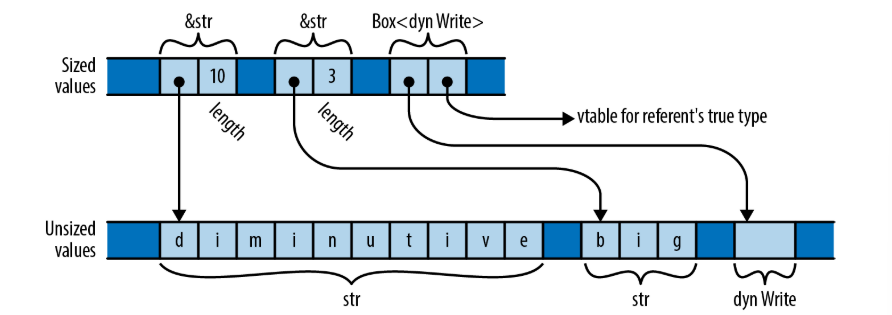
\includegraphics[width=0.8\textwidth]{../img/f13-1.png}
    \caption{指向大小不固定的值的引用}
    \label{f13-1}
\end{figure}

Rust中另一种常见的大小不固定类型是\texttt{dyn}类型,它是trait对象引用的目标。正如我们在“\nameref{traitobject}”中解释的一样,一个trait对象是一个指向实现了给定trait的值的指针。例如,类型\texttt{\&dyn std::io::Write}和\texttt{Box<dyn std::io::Write>}是指向实现了\texttt{Write} trait的值的指针。被引用的目标可能是一个文件或者网络套接字,或者是实现了\texttt{Write}的自定义类型。因为实现了\texttt{Write}的类型的集合是开放的,所以\texttt{dyn Write}也是大小不固定的类型:它的值可能有任意的大小。

Rust不能在变量中存储大小不固定的值或者将它们传递为参数。你只能通过指针例如\texttt{\&str}或\texttt{Box<dyn Write>}来处理它们,指针本身是固定大小的。正如\hyperref[f13-1]{表13-1}所示,一个指向大小不固定的值的指针总是一个\emph{胖指针(fat pointer)},占用两个字节:一个指向切片的指针加上切片的长度、一个trait对象加上一个指向方法实现的vtable的指针。

trait对象和切片的指针是对称的。在这两种情况下,都缺乏相应的类型信息:你不能在不知道\texttt{[u8]}长度的情况下索引它,也不能在不知道被指向的值的具体\texttt{Write}实现的情况下调用\texttt{Box<dyn Write>}的方法。在这两种情况下,胖指针填充了类型缺失的信息,加上了一个长度或者vtable的指针。被省略的静态信息被替换为了动态信息。

因为大小不固定的类型限制太多,所以大多数泛型类型参数都被限制为\texttt{Sized}类型。事实上,它几乎总是必须的,因此在Rust中它是默认的:如果你写\texttt{struct S<T> \{ ... \}},Rust认为你的意思是\texttt{struct S<T: Sized> \{ ... \}}。如果你不让\texttt{T}有这个约束,你必须显式写出来,即\texttt{struct S<T: ?Sized> \{ ... \}}。\texttt{?Sized}语法专门用于这种场景,含义是”不需要是\texttt{Sized}“。例如,如果你写了\texttt{struct S<T: ?Sized> \{ b: Box<T> \}},那么Rust将允许你写\texttt{S<Str>}和\texttt{S<dyn Write>},这时\texttt{b}将是一个胖指针;而\texttt{S<i32>}和\texttt{S<String>}中,\texttt{b}是一个普通指针。

抛开它们的限制不谈,大小不固定的类型让Rust的类型系统工作得更加顺畅。如果阅读标准库的文档,你偶尔会看到类型参数中的\texttt{?Sized}约束,这几乎总是意味着给定的类型只能被指向,同时允许相关的代码既能处理普通类型、又能处理切片和trait对象。当一个类型参数有\texttt{?Sized}约束时,人们通常会说它是\emph{可能大小不固定(questionably sized)}:它可能是\texttt{Sized},也可能不是。

除了切片和trait对象之外,还有另一种大小不固定的类型。一个结构体的最后一个字段(也只有最后一个字段)可能是大小不固定的,那么这个结构体本身也是大小不固定的。例如,\texttt{Rc<T>}引用计数指针内部被实现为私有类型\texttt{RcBox<T>}的指针,它存储了\texttt{T}和引用计数。这里有一个\texttt{RcBox}的简化版的定义:
\begin{minted}{Rust}
    struct RcBox<T: ?Sized> {
        ref_count: usize,
        value: T,
    }
\end{minted}

\texttt{value}字段就是\texttt{Rc<T>}引用的\texttt{T}值,\texttt{Rc<T>}解引用之后就是一个这个字段的指针。\texttt{ref\_count}字段保存引用计数。

真正的\texttt{RcBox}是标准库的实现细节,不能用于公开使用。但假设我们在处理一个上面的定义。你可以将\texttt{RcBox}和固定大小的类型一起使用,例如\texttt{RcBox<String>},结果将是一个固定大小的结构体类型。或者你可以将它和大小不固定的类型一起使用,例如\texttt{RcBox<dyn std::fmt::Display>}(其中\texttt{Display}表示可以被\texttt{println!}以及类似的宏格式化的类型),\texttt{RcBox<dyn Display>}是一个大小不固定的结构体类型。

你不能直接创建一个\texttt{RcBox<dyn Display>}值。你必须先创建一个普通的、固定大小的\texttt{RcBox},它的\texttt{value}字段的类型需要实现\texttt{Display},例如\texttt{RcBox<String>}。然后Rust允许你把一个它的引用\texttt{\&RcBox<String>}转换为胖指针引用\texttt{\&RcBox<dyn Display>}:
\begin{minted}{Rust}
    let boxed_lunch: RcBox<String> = RcBox {
        ref_count: 1,
        value: "lunch".to_string()
    };

    use std::fmt::Display;
    let boxed_displayable: &RcBox<dyn Display> = &boxed_lunch;
\end{minted}

当向函数传递参数时会隐式发生这个转换,因此你可以向接受\texttt{\&RcBox<dyn Display>}参数的函数传递一个\texttt{\&RcBox<String>}:
\begin{minted}{Rust}
    fn display(boxed: &RcBox<dyn Display>) {
        println!("For your enjoyment: {}", &boxed.value);
    }

    display(&boxed_lunch);
\end{minted}

这将会产生下列输出:
\begin{minted}{text}
    For your enjoyment: lunch
\end{minted}

\section{\texttt{Clone}}\label{clone}

\texttt{std::clone::Clone} trait用于那些可以拷贝自身的类型。\texttt{Clone}的定义如下:
\begin{minted}{Rust}
    trait Clone: Sized {
        fn clone(&self) -> Self;
        fn clone_from(&mut self, source: &Self) {
            *self = source.clone()
        }
    }
\end{minted}

\texttt{clone}方法应该构建一个\texttt{self}的独立拷贝并返回它。因为这个方法的返回类型是\texttt{Self},并且函数不能返回大小不固定的值,因此\texttt{Clone} trait扩展了\texttt{Sized} trait:它会约束实现的\texttt{Self}类型是\texttt{Sized}。

拷贝一个值通常意味着拷贝它拥有的所有内容,因此\texttt{clone}可能在时间和内存上的开销都比较大。例如,克隆一个\texttt{Vec<String>}不止要拷贝vector,还要拷贝它的每一个\texttt{String}元素。这就是为什么Rust不会自动拷贝值,而是要求你显式地调用方法来拷贝。引用计数指针例如\texttt{Rc<T>}和\texttt{Arc<T>}是例外:拷贝它们只会简单地递增引用计数并返回给你一个新的指针。

\texttt{clone\_from}方法将\texttt{self}修改为\texttt{source}的拷贝。\texttt{clone\_from}的默认实现简单地拷贝\texttt{source},然后将它移动进\texttt{*self}。这总是能正确工作,当对于某些类型,还有更快的方法达成相同的效果。例如,假设\texttt{s}和\texttt{t}都是\texttt{String}。语句\texttt{s = t.clone();}必须先克隆\texttt{t},drop掉\texttt{s}的旧值,然后将克隆的值移动进\texttt{s},因此这里面有一次堆分配和堆释放。但如果\texttt{s}原本的堆缓冲区有足够的容量存下\texttt{t}的内容,那么没有必要进行释放和分配操作:可以简单地将\texttt{t}的文本拷贝进\texttt{s}的缓冲区,然后调整它的长度。在泛型代码中,你应该使用\texttt{clone\_from},这样可以充分利用优化过的实现的优势。

如果你的类型的\texttt{Clone}实现只是简单地调用每一个字段或者元素的\texttt{clone}方法,然后利用这些克隆的值构造一个新的值,那么\texttt{clone\_from}的默认定义就已经够了,Rust将会为你实现它:只要在类型的定义上方加上\texttt{\#[derive(Clone)]}。

标准库中几乎所有应该能拷贝的类型都实现了\texttt{Clone}。基本类型例如\texttt{bool}和\texttt{i32}实现了。容器类型例如\texttt{String, Vec<T>, HashMap}也实现了。一些不应该能拷贝的类型例如\texttt{std::sync::Mutex}没有实现\texttt{Clone}。一些类型例如\texttt{std::fs::File}可以拷贝,但如果操作系统没有足够的资源那么拷贝可能会失败,这些类型也没有实现\texttt{Clone},因为\texttt{clone}不允许失败。作为替代,\texttt{std::fs::File}提供了一个\texttt{try\_clone}方法,它返回一个\texttt{std::io::Result<File>}来报告失败。

\section{\texttt{Copy}}\label{Copy}

在\hyperref[ch04]{第4章}中,我们解释过,对于大多数类型,赋值操作会移动它的值,而不是拷贝它们。移动值让我们可以更容易地追踪它们拥有的资源。但在“\nameref{copy}”中,我们指出了例外情况:不持有任何资源的简单类型可以是\texttt{Copy}类型,这种类型的赋值操作会拷贝源值,而不是移动值并把源值设为未初始化。

那个时候,我们并没有确切地说明\texttt{Copy}到底是什么,但现在我们可以告诉你:如果一个类型实现了\texttt{std::marker::Copy}标记trait,那么它就是\texttt{Copy}的,\texttt{Copy}的定义如下:
\begin{minted}{Rust}
    trait Copy: Clone { }
\end{minted}

很容易就可以为你自己的类型实现它:
\begin{minted}{Rust}
    impl Copy for MyType { }
\end{minted}

但因为\texttt{Copy}是一个有特殊含义的标记trait,所以Rust只允许可以通过逐字节的浅拷贝来拷贝自身的类型实现\texttt{Copy}。如果一个类型拥有任何其他资源,例如堆缓冲区或者操作系统句柄,那么它将不能实现\texttt{Copy}。

任何实现了\texttt{Drop} trait的类型不能实现\texttt{Copy}。Rust假定如果一个类型需要特殊的清理代码,那么它肯定也需要特殊的拷贝代码,所以不能是\texttt{Copy}。

和\texttt{Clone}一样,你可以使用\texttt{\#[derive(Copy)]}来让Rsut为你实现\texttt{Copy}。你通常能一次性看到它们两个,即\texttt{\#[derive(Copy, Clone)]}。

在将类型变为\texttt{Copy}之前请仔细思考。尽管这样做会让类型更容易使用,但却对类型本身的实现添加了很大的限制。而且隐式的拷贝可能会有很大的开销。我们已经在“\nameref{copy}”中详细解释了这些因素。

\section{\texttt{Deref}与\texttt{DerefMut}}\label{deref}

你可以通过实现\texttt{std::ops::Deref}和\texttt{std::ops::DerefMut} trait来指定解引用运算符\texttt{*}和\texttt{.}的行为。像\texttt{Box<T>}和\texttt{Rc<T>}这样的指针类型都实现了这些triat,因此它们的行为可以和Rust内建的指针类型一样。例如,如果你有一个\texttt{Box<Complex>}类型的值\texttt{b},那么\texttt{*b}就是\texttt{b}指向的\texttt{Complex}值,\texttt{b.re}就是它的实部。如果上下文赋值给被引用的对象,或者借用了被引用对象的可变引用,那么Rust会自动使用\texttt{DerefMut}(“可变地解引用”)trait;否则,只读的访问就已经足够了,所以它会使用\texttt{Deref}。

这个trait的定义类似于这样:
\begin{minted}{Rust}
    trait Deref {
        type Target: ?Sized;
        fn deref(&self) -> &Self::Target;
    }

    trait DerefMut: Deref {
        fn deref_mut(&mut self) -> &mut Self::Target;
    }
\end{minted}

\texttt{deref}和\texttt{deref\_mut}方法以\texttt{Self}的引用为参数,并返回\texttt{Self::Target}的引用。\texttt{Target}应该是\texttt{Self}包含、有用或指向的东西:对于\texttt{Box<Complex>},\texttt{Target}类型就是\texttt{Complex}。注意\texttt{DerefMut}扩展了\texttt{Deref}:如果你可以解引用某个值并修改它,那么你当然也应该能借用它的共享引用。因为方法返回一个和\texttt{\&self}生命周期相同的引用,只要返回的引用还存在,\texttt{self}就会保持被借用的状态。

\texttt{Deref}和\texttt{DerefMut} trait还扮演着另一个角色。因为\texttt{deref}以\texttt{Self}的引用作为参数并返回\texttt{Self::Target}的引用,所以Rust会自动把前者的类型转换为后者。换句话说,如果插入一个\texttt{deref}方法调用可以让类型变得匹配,那么Rust就会自动插入。实现\texttt{DerefMut}允许可变引用的相应转换。这些被称为\emph{强制解引用(deref coercions)}:一个类型被“强迫”表现得和另一个类型一样。

尽管你也可以自己显式写出转换来代替强制解引用,但它们确实很方便:
\begin{itemize}
    \item 如果你有一个\texttt{Rc<String>}的值\texttt{r},并想用它调用\texttt{String::find},你可以简单地写\texttt{r.find('?')}来代替\texttt{(*r).find('?')}:这个方法调用隐式地借用\texttt{r},\texttt{\&Rc<String>}被强迫为\texttt{\&String},因为\texttt{Rc<T>}实现了\texttt{Deref<Target=T>}。
    \item 你可以对\texttt{String}值使用类似\texttt{split\_at}的方法,即使\texttt{split\_at}是\texttt{str}切片类型的方法。因为\texttt{String}实现了\texttt{Deref<Target=str>}。没有必要让\texttt{String}重新实现\texttt{str}的所有方法,因为你可以把一个\texttt{\&String}强迫为一个\texttt{\&str}。
    \item 如果你有一个字节的vector \texttt{v},然后你想把它传递给一个接受\texttt{\&[u8]}字节序列的函数,那你只需要传递\texttt{\&v}作为参数,因为\texttt{Vec<T>}实现了\texttt{Deref<Target=[T]>}。
\end{itemize}

如果需要的话,Rust会尝试多次强制解引用。例如,使用上面提到的强制解引用,你可以直接用\texttt{Rc<String>}调用\texttt{split\_at}方法,因为\texttt{\&Rc<String>}解引用为\texttt{\&String},它再解引用为\texttt{\&str},而\texttt{\&str}有\texttt{split\_at}方法。

例如,假设你有下面的类型:
\begin{minted}{Rust}
    struct Selector<T> {
        /// 这个`Selector`中可用的元素
        elements: Vec<T>,

        /// 当前的元素在`elements`中的索引。
        /// 一个`Selector`的行为类似于当前的元素的指针。
        current: usize
    }
\end{minted}

为了让\texttt{Selector}的行为像文档中声明的一样,你必须为它实现\texttt{Deref}和\texttt{DerefMut}:
\begin{minted}{Rust}
    use std::ops::{Deref, DerefMut};

    impl<T> Deref for Selector<T> {
        type Target = T;
        fn deref(&self) -> &T {
            &self.elements[self.current]
        }
    }

    impl<T> DerefMut for Selector<T> {
        fn deref_mut(&mut self) -> &mut T {
            &mut self.elements[self.current]
        }
    }
\end{minted}

有了上面的视线之后,你可以像这样使用一个\texttt{Selector}:
\begin{minted}{Rust}
    let mut s = Selector { elements: vec!['x', 'y', 'z'],
                           current: 2 };

    // 因为`Selector`实现了`Deref`,我们可以使用`*`运算符来
    // 引用它的当前的元素。
    assert_eq!(*s, 'z');

    // 断言`z`是字母,通过强制解引用直接在`Selector`上调用`char`的方法
    assert!(s.is_alphabetic());

    // 通过给`Selector`的引用赋值把'z'改为'w'。
    *s = 'w';

    assert_eq!(s.elements, ['x', 'y', 'w']);
\end{minted}

\texttt{Deref}和\texttt{DerefMut} trait是为智能指针例如\texttt{Box, Rc, Arc},以及那些经常以引用的方式使用并且充当另一种类型的类型准备的,例如\texttt{Vec<T>}和\texttt{String}充当\texttt{[T]}和\texttt{str}。你不应该仅仅为了让一个类型能自动使用\texttt{Target}类型的方法(类似于C++的子类可以使用基类的方法)而实现\texttt{Deref}和\texttt{DerefMut}。这可能不会按照你预想的工作,并且当事情变得复杂时可能会变得令人迷惑。

强制解引用有时可能会导致困惑:Rust使用它们来解决类型冲突,但不把它们用于满足类型变量的约束。例如,下面的代码可以正常工作:
\begin{minted}{Rust}
    let s = Selector { elements: vec!["good", "bad", "ugly"],
                       current: 2};
    fn show_it(thing: &str) { println!("{}", thing); }
    show_it(&s);
\end{minted}

在调用\texttt{show\_it(\&s)}中,Rust看到了一个\texttt{\&Selector<\&str>}类型的实参,和一个\texttt{\&str}类型的形参,然后它发现了\texttt{Deref<Target=str>}实现,并根据需要把调用重写为\texttt{show\_it(s.deref())}。

然而,如果你把\texttt{show\_it}改为一个泛型函数,Rust突然变得不配合了:
\begin{minted}{Rust}
    use std::fmt::Display;
    fn show_it_generic<T: Display>(thing: T) { println!("{}", thing); }
    show_it_generic(&s);
\end{minted}

Rust会报错:
\begin{minted}{text}
    error: `Selector<&str>` doesn't implement `std::fmt::Display`
        |
     33 |     fn show_it_generic<T: Display>(thing: T) { println!("{}", thing); }
        |                           ------- required by this bound in
        |                                   `show_it_generic`
     34 |     show_it_generic(&s);
        |                     ^^
        |                     |
        |                     `Selector<&str>` cannot be formatted with the
        |                     default formatter
        |                     help: consider adding dereference here: `&*s`
        |
\end{minted}

这可能看起来非常奇怪:为什么把函数改为泛型的就会导致这么一个错误?事实上,\texttt{Selector<\&str>}自身没有实现\texttt{Display},但它可以解引用成\texttt{\&str},后者实现了。

因为你传递了一个\texttt{\&Selector<\&str>}类型的参数,而函数的形参类型是\texttt{\&T},因此类型参数\texttt{T}必须是\texttt{Selector<\&str>}。然后,Rust会检查\texttt{T: Display}约束是否满足:因为Rust不会使用强制解引用来满足类型参数的约束,所以检查会失败。

为了解决这个问题,你可以使用\texttt{as}运算符显式转换:
\begin{minted}{Rust}
    show_it_generic(&s as &str);
\end{minted}

或者,像编译器建议的一样,你可以使用\texttt{\&*}来强制解引用:
\begin{minted}{Rust}
    show_it_generic(&*s);
\end{minted}

\section{\texttt{Default}}\label{default}

一些类型会有一些有意义的默认值:vecotr或string的默认值就是空,默认的数字是0,默认的\texttt{Option}是\texttt{None},等等。这样的类型可以实现\texttt{std::default::Default} trait:
\begin{minted}{Rust}
    trait Default {
        fn default() -> Self;
    }
\end{minted}

\texttt{default}方法简单地返回一个\texttt{Self}类型的新值。例如,\texttt{String}的\texttt{Default}实现非常的直观:
\begin{minted}{Rust}
    impl Default for String {
        fn default() -> String {
            String::new()
        }
    }    
\end{minted}

Rust的所有集合类型——\texttt{Vec, HashMap, BinaryHeap}等都实现了\texttt{Default},它们的\texttt{default()}方法都返回一个空的集合。当你需要创建一个集合来存储一些值,但你希望代码的调用者来决定创建什么类型的集合时这会非常有用。例如,\texttt{Iterator} trait的\texttt{partition}方法把迭代器产生的值划分为两个集合,使用一个闭包来决定每个值被分到哪个集合:
\begin{minted}{Rust}
    use std::collections::HashSet;
    let squares = [4, 9, 16, 25, 36, 49, 64];
    let (powers_of_two, impure): (HashSet<i32, HashSet<i32>)
        = squares.iter().partition(|&n| n & (n-1) == 0);
    
    assert_eq!(powers_of_two.len(), 3);
    assert_eq!(impure.len(), 4);
\end{minted}

闭包\texttt{|\&n| n \& (n-1) == 0}使用了位操作来分辨一个数字是不是2的幂,\texttt{partition}使用它来产生两个\texttt{HashSet}。当然,\texttt{partition}并不是只能用于\texttt{HashSet},你可以用它产生任何类型的集合,只要这个集合实现了\texttt{Default}来创建空的集合,以及\texttt{Extend<T>}来像集合中添加一个\texttt{T}类型的值。\texttt{String}实现了\texttt{Default}和\texttt{Extend<char>},所以你可以写:
\begin{minted}{Rust}
    let (upper, lower): (String, String)
        = "Great Teacher Onizuka".chars().partition(|&c| c.is_uppercase());
    assert_eq!(upper, "GTO");
    assert_eq!(lower, "reat eacher nizuka");
\end{minted}

\texttt{Default}的另一个常见用法是为一个结构体生成默认值,它代表一些固定的参数的集合。例如,\texttt{glium} crate为强大且复杂的OpenGL图形库提供Rust绑定。\texttt{glium::DrawParameters}结构体包含24个字段,每一个字段都控制一部分OpenGL渲染图形位的细节。\texttt{glium}里的\texttt{draw}函数接受一个\texttt{DrawParameters}结构体作为参数。因为\texttt{DrawParameters}实现了\texttt{Default},你可以创建一个默认的值,然后只修改想要修改的字段,最后传给\texttt{draw}:
\begin{minted}{Rust}
    let params = glium::DrawParameters {
        line_width: Some(0.02),
        point_size: Some(0.02),
        .. Default::default()
    };

    target.draw(..., &params).unwrap();
\end{minted}

\texttt{Default::default()}调用创建了一个\texttt{DrawParameters}的默认值,然后使用\texttt{..}语法创建一个新的只有\texttt{line\_width}和\texttt{point\_size}字段改变了的新值,最后把它传给\texttt{target.draw}。

如果一个类型\texttt{T}实现了\texttt{Default},那么标准库会自动为\texttt{Rc<T>}、\texttt{Arc<T>}、\texttt{Box<T>}、\texttt{Cell<T>}、\texttt{RefCell<T>}、\texttt{Cow<T>}、\texttt{Mutex<T>}、\texttt{RwLock<T>}实现\texttt{Default}。例如,\texttt{Rc<T>}类型的默认值,是一个类型\texttt{T}的默认值的\texttt{Rc}指针。

如果一个元组类型的所有元素的类型都实现了\texttt{Default},那么元组也会自动实现\texttt{Default},它的默认值就是每个元素的默认值组成的元组。

Rust不会隐式为结构体类型实现\texttt{Default},但如果一个结构体的所有字段都实现了\texttt{Default},你可以使用\texttt{\#[derive(Default)]}来为结构体自动生成\texttt{Default}。

\section{\texttt{AsRef}与\texttt{AsMut}}\label{asref}

如果一个类型实现了\texttt{AsRef<T>},那么意味着你可以从它高效地借用一个\texttt{\&T}。\texttt{AsMut}用于可变引用。它们的定义如下:
\begin{minted}{Rust}
    trait AsRef<T: ?Sized> {
        fn as_ref(&self) -> &T;
    }

    trait AsMut<T: ?Sized> {
        fn as_mut(&mut self) -> &mut T;
    }
\end{minted}

例如,\texttt{Vec<T>}实现了\texttt{AsRef<[T]>},\texttt{String}实现了\texttt{AsRef<str>}。你可以从一个\texttt{String}的内容借用一个字节的数组,因为\texttt{String}也实现了\texttt{AsRef<[u8]>}。

\texttt{AsRef}通常用于让函数在接受参数时更加灵活。例如,\texttt{std::fs::File::open}函数的声明如下:
\begin{minted}{Rust}
    fn open<P: AsRef<Path>>(path: P) -> Result<File>
\end{minted}

\texttt{open}真正想要的是一个\texttt{\&Path},这个类型表示一个文件系统路径。但有了这个签名以后,\texttt{open}接受任何可以被借用一个\texttt{\&Path}的类型——也就是说,实现了\texttt{AsRef<Path>}的任何类型。这样的类型包括\texttt{String}和\texttt{str},操作系统接口字符串类型\texttt{OsString}和\texttt{OsStr}、当然还有\texttt{PathBuf}和\texttt{Path}。完整的列表见标准库的文档。它允许你向\texttt{open}传递字符串字面量:
\begin{minted}{Rust}
    let dot_emacs = std::fs::File::open("/home/jimb/.emacs")?;
\end{minted}

标准库中所有的文件系统函数都用这种方式接受路径参数。对于调用者来说,它的作用就像是C++中重载的函数一样,尽管Rust用了不同的方法来表示可以接受哪些类型的参数。

但只有这些还不够。一个字符串字面量是一个\texttt{\&str},但实现了\texttt{AsRef<Path>}的类型是\texttt{str},没有\texttt{\&}。正如我们在“\nameref{deref}”一节中解释的一样,Rust不会尝试通过强制解引用来满足类型参数的约束,因此它们也不能解决这个问题。

幸运的是,标准库中包含了全面的实现:
\begin{minted}{Rust}
    impl<'a, T, U> AsRef<U> for &'a T
        where T: AsRef<U>,
              T: ?Sized, U: ?Sized
    {
        fn as_ref(&self) -> &U {
            (*self).as_ref()
        }
    }
\end{minted}

换句话说,对于任意的类型\texttt{T}和\texttt{U},如果有\texttt{T: AsRef<U>},那么也会有\texttt{\&T: AsRef<U>}:简单地先解引用然后就和之前一样继续。这里,因为有\texttt{str: AsRef<Path>},所以也会有\texttt{\&str: AsRef<Path>}。某种意义上,这是一种在检查类型参数中的\texttt{AsRef}约束时受限的强制解引用方式。

你可能会假设如果一个类型实现了\texttt{AsRef<T>},那它也应该实现\texttt{AsMut<T>}。然而,还有一些不适合这样的情况。例如,我们提到过\texttt{String}实现了\texttt{AsRef<[u8]>};这是有意义的,因为每一个\texttt{String}都包含一个字节缓冲区,可以被当做二进制数据访问。然而,\texttt{String}还保证这些字节是有效的UTF-8文本;如果\texttt{String}实现了\texttt{AsMut<[u8]>},那么调用者将能把\texttt{String}的字节缓冲区修改为任何内容,那么你将不能再信任\texttt{String}里存储的是有效的UTF-8。只有那些修改返回的\texttt{T}不会破坏一致性的类型实现\texttt{AsMut<T>}才有意义。

尽管\texttt{AsRef}和\texttt{AsMut}非常简单,但它提供了一种标准化、泛型的方式来进行引用转换,进而避免了更多特化的转换trait。当实现\texttt{AsRef<Foo>}就足够的时候,你应该避免实现你自己的\texttt{AsFoo} trait。


\section{\texttt{Borrow}与\texttt{BorrowMut}}\label{borrow}

\texttt{std::borrow::Borrow} trait和\texttt{AsRef}很相似:如果一个类型实现了\texttt{Borrow<T>},那么它的\texttt{borrow}方法可以高效地借用一个\texttt{\&T}。但\texttt{Borrow}有更多的限制:只有当借用的\texttt{\&T}和被借用的值的哈希值和比较方式相同时,这个类型才应该实现\texttt{Borrow<T>}。(Rust并不强迫这一点,这只是这个trait被设计的意图。)这让\texttt{Borrow}在处理哈希表和树的key时非常有用,在处理其他可能会被哈希或者比较的值也很有用。

当从\texttt{String}借用时,这种不同很重要,例如:\texttt{String}实现了\texttt{AsRef<str>}、\texttt{AsRef<[u8]>}、\texttt{AsRef<Path>},但这三种类型会有不同的哈希值。只有\texttt{\&str}保证和等价的\texttt{String}有相同的哈希值,因此\texttt{String}只实现了\texttt{Borrow<str>}。

\texttt{Borrow}的定义和\texttt{AsRef}的定义几乎完全相同,只有名字变了:
\begin{minted}{Rust}
    trait Borrow<Borrowed: ?Sized> {
        fn borrow(&self) -> &Borrow;
    }
\end{minted}

\texttt{Borrow}被设计用来解决泛型哈希表和其他关联集合类型的特性问题。例如,假设你有一个\texttt{std::collections::HashMap<String, i32>},把字符串映射到数字。这个表的key是\texttt{String},所以每一个表项都拥有一个\texttt{String}。那么在一个这样的表中查找一个表项的方法的签名应该是什么样的?这是第一次尝试:
\begin{minted}{Rust}
    impl<K, V> HashMap<K, V> where K: Eq + Hash
    {
        fn get(&self, key: K) -> Option<&V> { ... }
    }
\end{minted}

这么做是有道理的:为了查找一个表项,你必须提供一个和表的key相同的类型。但在这个情况中,\texttt{K}是\texttt{String},这样的签名会强迫你每次调用\texttt{get}时以值传递一个\texttt{String},显然这很浪费。你实际上只需要一个key的引用:
\begin{minted}{Rust}
    impl<K, V> HashMap<K, V> where K: Eq + Hash
    {
        fn get(&self, key: &K) -> Option<&V> { ... }
    }
\end{minted}

这样好一点,但你现在必须传递\texttt{\&String}作为key,所以如果你想查找一个常量字符串,你必须这么写:
\begin{minted}{Rust}
    hashtable.get(&"twenty-two".to_string());
\end{minted}

这显然很离谱:它在堆上分配了一个\texttt{String}的缓冲区并把文本拷贝进去,然后借用它得到一个\texttt{\&String},传给\texttt{get}之后再drop掉。

如果可以传递任何可以被哈希或者可以与key比较的类型,那么显然会更好。例如,例如,一个\texttt{\&str}完美满足条件。因此这是最终的版本,你可以在标准库中找到它:
\begin{minted}{Rust}
    impl<K, V> HashMap<K, V> where K: Eq + Hash
    {
        fn get<Q: ?Sized>(&self, key: &Q) -> Option<&V>
            where K: Borrow<Q>,
                  Q: Eq + Hash
        { ... }
    }
\end{minted}

换句话说,如果你可以将一个表项的key借用为一个\texttt{\&Q},并且引用的哈希值和比较结果就和用key本身所得的结果一样,那么\texttt{\&Q}就是一个可以接受的key类型。因此\texttt{String}实现了\texttt{Borrow<str>}和\texttt{Borrow<String>},\texttt{get}的最终版本允许你传递\texttt{\&String}或者\texttt{\&str}作为key。

\texttt{Vec<T>}和\texttt{[T; N]}实现了\texttt{Borrow<[T]>}。每一个类似字符串的类型都允许借用相应的切片类型:\texttt{String}实现了\texttt{Borrow<str>},\texttt{PathBuf}实现了\texttt{Borrow<Path>},等等。所有标准库的关联集合类型都使用了\texttt{Borrow}来决定哪些类型可以被传入查找函数。

标准库包含了完备的实现,因此每一个类型\texttt{T}都可以从它自身借用:\texttt{T: Borrow<T>}。这保证了在一个\texttt{HashMap<K, V>}中查找表项时\texttt{\&K}总是可接受的类型。

为了方便,每一个\texttt{\&mut T}类型也实现了\texttt{Borrow<T>},返回一个共享引用\texttt{\&T}。这允许你直接向集合的查找函数传递可变引用,不需要重新借用共享引用,它模拟了Rust通常把可变引用转换为共享引用的隐式强制解引用。

\texttt{BorrowMut} trait是\texttt{Borrow}的可变引用版本:
\begin{minted}{Rust}
    trait BorrowMut<Borrowed: ?Sized>: Borrow<Borrowed> {
        fn borrow_mut(&mut self) -> &mut Borrowed;
    }
\end{minted}

\texttt{Borrow}应该满足的条件也适用于\texttt{BorrowMut}。

\section{\texttt{From}与\texttt{Into}}\label{from}

\texttt{std::convert::From}和\texttt{std::convert::Into} trait代表消耗一个值并返回另一个值的转换。与\texttt{AsRef}和\texttt{AsMut} trait从一个类型借用另一个类型的引用不同,\texttt{From}和\texttt{Into}会获取参数的所有权,对它进行变换,然后把最后的结果的所有权返回给调用着。

它们的定义完美对称:
\begin{minted}{Rust}
    trait Into<T>: Sized {
        fn into(self) -> T:
    }

    trait From<T>: Sized {
        fn from(other: T) -> Self;
    }
\end{minted}

标准库自动实现每一个类型到自身的转换:每个类型\texttt{T}都实现了\texttt{From<T>}和\texttt{Into<T>}。

尽管这两个trait看起来像是提供了两种不同的方式做同一件事情,但实际上它们用不同的用途。

通常使用\texttt{Into}来让函数可以更灵活的接收参数。例如,如果你写:
\begin{minted}{Rust}
    use std::net::Ipv4Addr;
    fn ping<A>(address: A) -> std::io::Result<bool>
        where A: Into<Ipv4Addr>
    {
        let ipv4_address = address.into();
        ...
    }
\end{minted}

那么\texttt{ping}不止可以接受\texttt{Ipv4Addr}作为参数,还可以接受一个\texttt{u32}或者一个\texttt{[u8; 4]}数组,因为这些类型都实现了\texttt{Into<Ipv4Addr>}。(有时把IPv4地址当成单个32位整数或者一个四个字节的数组会很有用)因为\texttt{ping}唯一知道的就是\texttt{address}实现了\texttt{Into<Ipv4Addr>},所以当你调用\texttt{into}时没有必要指明你想要什么类型。只有一种类型可能成功,所以类型推导会自动为你填充它。

类似于上一节的\texttt{AsRef},它的效果也很像C++中的重载函数。有了上面的\texttt{ping}定义,我们可以像下面这样调用:
\begin{minted}{Rust}
    println!("{:?}", ping(Ipv4Addr::new(23, 21, 68, 141))); // 传递一个Ipv4Addr
    println!("{:?}", ping([66, 146, 219, 98]));             // 传递一个[u8; 4]
    println!("{:?}", ping(0xd076eb94_u32));                 // 传递一个u32
\end{minted}

\texttt{From} trait则扮演不同的角色。\texttt{from}方法充当泛型的构造函数,从别的值构造一个该类型的实例。例如,\texttt{Ipv4Addr}简单地实现了\texttt{From<[u8;4]>}和\texttt{From<u32>},而不是定义两个名叫\texttt{from\_array}和\texttt{from\_u32}的方法:
\begin{minted}{Rust}
    let addr1 = Ipv4Addr::from([66, 146, 219, 98]);
    let addr2 = Ipv4Addr::from(0xd076eb94_u32);
\end{minted}

我们可以让类型推导来决定使用哪个实现。

给定一个合适的\texttt{From}实现,标准库会自动生成相应的\texttt{Into} trait的实现。当你定义自己的类型时,如果它需要单个参数的构造函数,你可以将它写成\texttt{From<T>}的实现,而不是定义一个新的构造函数。你可以免费得到相应的\texttt{Into}实现。

因为\texttt{from}和\texttt{into}转换会获取参数的所有权,转换可以重用原始值的资源来构造转换后的值。例如,假设你写了:
\begin{minted}{Rust}
    let text = "Beautiful Soup".to_string();
    let bytes: Vec<u8> = text.into();
\end{minted}

\texttt{String}的\texttt{Into<Vec<u8>>}的实现简单地获取\texttt{String}的堆缓冲区的所有权,并重用它作为返回的vector的元素缓冲区。这个转换中不需要分配或拷贝文本。这是另一个使用move来实现高效的方法的例子。

这些转换还提供了一种很好的方式来放松类型的约束,灵活的同时又没有减弱被约束类型的保证。例如,一个\texttt{String}保证它的内容总是有效的UTF-8;它的方法都有很谨慎的限制,来保证你不能引入无效的UTF-8。但这个例子高效地把一个\texttt{String}转换成了一个普通的字节块,你可以对它做任何事:也许你准备压缩它,或者将它和其他不是UTF-8的二进制数据混合。因为\texttt{into}会获取参数的所有权,转换之后\texttt{text}将变为未初始化,这意味着我们可以自由地访问之前的\texttt{String}的缓冲区,而不需要破坏任何现有的\texttt{String}。

然而,低开销的转换并不是\texttt{Into}和\texttt{From}的约定的一部分。与\texttt{AsRef}和\texttt{AsMut}被期望开销很小不同,\texttt{From}和\texttt{Into}转换可能会分配、赋值、或者处理值的内容。例如,String实现了\texttt{From<\&str>},它把字符串切片拷贝到\texttt{String}分配的新的堆上的缓冲区。还有\texttt{std::collections::BinaryHeap<T>}实现了\texttt{From<Vec<T>>},它根据算法的要求对元素进行比较和重新排序。

\texttt{?}运算符使用\texttt{From}和\texttt{Into}通过按需将特定的错误类型自动转换为通用的错误类型来帮忙处理函数中可能会失败的代码。

例如,想象一个系统需要读取二进制数据并把其中一部分被写作UTF-8文本的10进制数字转换回数字。这意味着要使用\texttt{std::str::from\_utf8}和\texttt{i32}的\texttt{FromStr}实现,它们可能会返回不同类型错误。假设我们使用了在\hyperref[ch07]{第7章}中定义的\texttt{GenericError}和\texttt{GenericResult}类型,那么\texttt{?}运算符将会为我们做这个转换:
\begin{minted}{Rust}
    type GenericError = Box<dyn std::error::Error + Send + Sync + 'static>;
    type GenericResult<T> = Result<T, GenericError>;

    fn parse_i32_bytes(b: &[u8]) -> GenericResult<i32> {
        Ok(std::str::from_utf8(b)?.parse::<i32>()?)
    }
\end{minted}

类似大多数错误类型,\texttt{Utf8Error}和\texttt{ParseIntError}实现了\texttt{Error} trait,并且标准库给了我们完备的\texttt{From impl}来把任何实现了\texttt{Error}的类型转换为\texttt{Box<dyn Error>},\texttt{?}将会自动使用它:
\begin{minted}{Rust}
    impl<'a, E: Error + Send + Sync + 'a> From<E>
        for Box<dyn Error + Send + Sync + 'a> {
            fn from(err: E) -> Box<dyn Error + Send + Sync + 'a> {
                Box::new(err)
            }
        }
\end{minted}

它将原本需要两个\texttt{match}语句的复杂函数转变为只需要一行。

在\texttt{From}和\texttt{Into}被添加进标准库中之前,Rust代码中充满了单独的转换trait和构造方法,每一个都用于单个类型。\texttt{From}提供了标准的转换方式,你可以使用他们来让你的类型更加易于使用,因为你的用户已经对它们很熟悉了。其他的库和语言本身也可以使用这些trait作为约定的、标准的方式来处理转换。

\texttt{From}和\texttt{Into}是不可失败的trait——它们的API要求转换不能失败。不幸的是,很多转换更加复杂。例如,大整数例如\texttt{i64}可以存储比\texttt{i32}大很多的数字,将一个类似\texttt{2\_000\_000\_000\_000i64}这样的数字转换为\texttt{i32}没有意义。如果直接把前32位丢掉,那么并不会总是返回我们期望的结果:
\begin{minted}{Rust}
    let huge = 2_000_000_000_000i64;
    let smaller = huge as i32;
    println!("{}", smaller);    // -1454759936
\end{minted}

有很多处理这种问题的方法。取决于上下文,这种“折断”的方式也可能很合适。另一方面,数字信号处理和控制系统等应用通常可以使用“饱和”转换:超过最大可表示的值的数字会被限制为可表示的最大值。

\section{\texttt{TryFrom}与\texttt{TryInto}}\label{tryfrom}

因为这种转换到底该怎么做并不是很清楚,所以Rust并没有为\texttt{i32}实现\texttt{From<i64>},也没有实现任何其他可能丢失信息的数制转换。作为代替,\texttt{i32}实现了\texttt{TryFrom<i64>}。\texttt{TryFrom}和\texttt{TryInto}是\texttt{From}和\texttt{Into}的可能失败的版本,实现\texttt{TryFrom}意味着\texttt{TryInto}也会自动实现。

它们的定义只比\texttt{From}和\texttt{Into}复杂一点:
\begin{minted}{Rust}
    pub trait TryFrom<T>: Sized {
        type Error;
        fn try_from(value: T) -> Result<Self, Self::Error>;
    }

    pub trait TryInto<T>: Sized {
        type Error;
        fn try_into(self) -> Result<T, Self::Error>;
    }
\end{minted}

\texttt{try\_into()}方法返回一个\texttt{Result},因此我们可以选择在失败的情况下做什么,例如一个数字太大不能存放在结果类型中:
\begin{minted}{Rust}
    use std::convert::TryInto;
    // 溢出时选择饱和,而不是折断
    let smaller: i32 = huge.try_into().unwrap_or(i32::MAX);
\end{minted}

如果我们想同时处理负数的情况,我们可以使用\texttt{Result}的\texttt{unwrap\_or\_else()}的方法:
\begin{minted}{Rust}
    let smaller: i32 = huge.try_into().unwrap_or_else(|_| {
        if huge >= 0 {
            i32::MAX
        } else {
            i32::MIN
        }
    });
\end{minted}

为你自己的类型实现可能失败的转换也非常简单。\texttt{Error}类型可以简单,也可以像某个应用的需求一样复杂。这里标准库使用了一个空的结构体,没有提供转换失败的原因相关的信息,因为唯一可能失败的原因就是溢出。另一方面,在更复杂的类型之间转换可能会需要返回更多的信息:
\begin{minted}{Rust}
    impl TryInto<LinearShift> for Transform {
        type Error = TransformError;

        fn try_into(self) -> Result<LinearShift, Self::Error> {
            if !self.normalized() {
                return Err(TransformError::NotNormalized);
            }
            ...
        }
    }
\end{minted}

\texttt{From}和\texttt{Into}将只需要简单的转换的类型联系起来,\texttt{TryFrom}和\texttt{TryInto}用\texttt{Rusult}的强大的错误处理能力扩展了\texttt{From}和\texttt{Into}的简单转换。这四个trait可以一起使用来联系一个crate中的多种类型。

\section{\texttt{ToOwned}}\label{toowned}




    \chapter{闭包}\label{ch14}

\emph{Save the environment! Create a closure today!}

\begin{flushright}
    ——Cormac Flanagan
\end{flushright}

排序一个整数的vector非常简单:
\begin{minted}{Rust}
    integers.sort();
\end{minted}

然而一个悲伤的事实是,当我们想要对一些数据排序时,它们基本从来都不只是整数。我们通常要排序某种记录,内建的\texttt{sort}方法通常不能工作:
\begin{minted}{Rust}
    struct City {
        name: String,
        population: i64,
        country: String,
        ...
    }

    fn sort_cities(cities: &mut Vec<City>) {
        cities.sort();  // 错误:你想让它们怎么排序?
    }
\end{minted}

Rust会报错\texttt{City}没有实现\texttt{std::cmp::Ord}。我们需要像这样指明排序的顺序:
\begin{minted}{Rust}
    /// 按照人口排序城市的辅助函数
    fn city_population_descending(city: &City) -> i64 {
        -city.population
    }

    fn sort_cities(cities: &mut Vec<City>) {
        cities.sort_by_key(city_population_descending); // ok
    }
\end{minted}

这个辅助函数\texttt{city\_population\_descending},获取一个\texttt{City}记录并提取出\emph{key},我们根据这个字段来排序数据。(它返回一个负数是因为\texttt{sort}以递增顺序排序,但我们想以降序排序:人多最多的城市优先。)\texttt{sort\_by\_key}方法以这个返回key的函数为参数。

这可以工作的很好,当如果将辅助函数写成一个\emph{闭包(closure)}(一个匿名的函数表达式)会更简洁:
\begin{minted}{Rust}
    fn sort_cities(cities: &mut Vec<City>) {
        cities.sort_by_key(|city| -city.population);
    }
\end{minted}

这里的闭包是\texttt{|city| -city.population}。它有一个参数\texttt{city},然后返回\texttt{-city.population}。Rust会从闭包的使用中推断出参数和返回值的类型。

标准库中其他接受闭包的特性的例子包括:
\begin{itemize}
    \item \texttt{Iterator}的方法例如\texttt{map}和\texttt{filter}。我们将在\hyperref[ch15]{第15章}介绍这些方法。
    \item 线程的API例如\texttt{thread::spawn},它会创建一个新的系统线程。并发就是把工作移动到其他的线程,闭包能方便的表示这种工作单元。我们将在\hyperref[ch19]{第19章}中介绍这些特性。
    \item 一些需要根据条件计算默认值的方法,例如\texttt{HashMap}条目的\texttt{or\_insert\_with}方法。这个方法获取一个\texttt{HashMap}的表项,或者创建一个表项,当计算默认值有很大开销时会使用这个方法。只有当必须创建一个新表项的时候作为闭包传入的默认值才会被调用。
\end{itemize}

当然,现在匿名函数随处可见,即使像Java、C\#、Python、C++这些一开始没有的语言现在也有了。从现在开始我们将假设你已经见过匿名函数,并专注于介绍Rust的闭包的独特之处。本章中,你将学习到三种不同类型的闭包、如何将闭包和标准库方法一起使用、一个闭包如何“捕获”作用域内的变量、如何编写自己的以闭包为参数的函数和方法、以及如何存储闭包以待之后用于回调。我们将解释Rust的闭包是怎么实现的,以及为什么它们比你想象的更加快速。

\section{捕获变量}
一个闭包可以使用封闭函数内的数据。例如:
\begin{minted}{Rust}
    /// 根据统计数据排序
    fn sort_by_statistic(cities: &mut Vec<City>, stat: Statistic) {
        cities.sort_by_key(|city| -city.get_statistic(stat));
    }
\end{minted}

这里的闭包使用了\texttt{stat},它属于当前的封闭函数\texttt{sort\_by\_statistic}。我们说这个闭包“捕获”了\texttt{stat}。这是闭包最经典的特性之一。Rust自然支持它,但在Rust中,这个特性有很多需要注意的地方。

在大多数有闭包的语言中,垃圾收集扮演了重要的角色。例如,考虑这段JavaScript代码:
\begin{minted}{Rust}
    // 开始一段动画,重新排序表格中的城市
    function startSortingAnimation(cities, stat) {
        // 排序表格时用到的辅助函数。
        // 注意这个函数用到了stat
        function keyfn(city) {
            return city.get_statistic(stat);
        }

        if (pendingSort)
            pendingSort.cancel();

        // 现在开始动画,向它传递keyfn。
        // 排序算法之后将会调用keyfn。
        pendingSort = new SortingAnimation(cities, keyfn);
    }
\end{minted}

这个闭包\texttt{keyfn}被存储在新的\texttt{SortingAnimation}对象中。这意味着它可能会在\texttt{startSortingAnimation}返回之后被调用。通常来讲当一个函数返回时,它的所有变量和参数都会离开作用域并且被丢弃。但这里,JavaScript引擎必须一直保持\texttt{stat},因为闭包中用到了它。大多数JavaScript引擎通过在堆上分配\texttt{stat},然后让垃圾收集器之后再回收它来做到这一点。

Rust没有垃圾收集。那么这样的代码会如何运作?为了回答这个问题,我们先看两个例子。

\subsection{借用值的闭包}
首先,让我们重复这一节开始时的例子:
\begin{minted}{Rust}
    /// 根据统计数据排序
    fn sort_by_statistic(cities: &mut Vec<City>, stat: Statistic) {
        cities.sort_by_key(|city| -city.get_statistic(stat));
    }
\end{minted}

在这个例子中,当Rust创建闭包时,它会自动自动借用一个\texttt{stat}的引用。按理来说,闭包用到了\texttt{stat},所以它必须有一个指向它的引用。

剩余的部分就很简单了。闭包仍然遵循我们在\hyperref[ch05]{第5章}中介绍的有关借用和生命周期的规则。另外,因为闭包包含一个\texttt{stat}的引用,所以Rust不允许它比\texttt{stat}活得更长。因为这个闭包只在排序中使用,所以这个例子没有问题。

简单来说,Rust通过使用生命周期代替垃圾收集来保证安全性。Rust的方式更加快速:即使是一个很快的GC分配器也比Rust这种把\texttt{stat}存在栈上的方式慢。

\subsection{偷取值的闭包}
第二个例子更加棘手:
\begin{minted}{Rust}
    use std::thread;

    fn start_sorting_thread(mut cities: Vec<City>, stat: Statistic) -> thread::JoinHandle<Vec<City>>
    {
        let key_fn = |city: &City| -> i64 { -city.get_statistic(stat) };

        thread::spawn(|| {
            cities.sort_by_key(key_fn);
            cities
        })
    }
\end{minted}

这和我们上面的JavaScript的例子有一些像:\texttt{thread::spawn}获取闭包并且在一个新的系统线程中调用它。注意\texttt{||}是闭包的空参数列表。

新的线程和调用者并行运行。当闭包返回时,新的线程也会退出。(闭包的返回值会通过一个\texttt{JoinHandle}值返还给调用者。我们将在\hyperref[ch19]{第19章}中讨论它)。

闭包\texttt{key\_fn}仍然包含一个\texttt{stat}的引用。但这一次,Rust不能保证引用会被安全使用。因此Rust会拒绝这个程序:
\begin{minted}{text}
    error[E0373]: closure may outlive the current function, but it borrows `stat`,
                  which is owned by the current function
      --> closures_sort_thread.rs:33:18
       |
    33 | let key_fn = |city: &City| -> i64 { -city.get_statistic(stat) };
       |              ^^^^^^^^^^^^^^^^^^^^                       ^^^^
       |              |                                      `stat` is borrowed here
       |              may outlive borrowed value `stat`
\end{minted}

事实上,这里有两个问题,因为\texttt{cities}也被不安全地共享。简单来说,\texttt{thread::spawn}新创建的线程不能保证在\texttt{cities}和\texttt{stat}在离开函数被销毁之前完成工作。

解决这两个问题的方法是一样的:告诉Rust把\texttt{cities}和\texttt{stat}\emph{移动(move)}进新的闭包,而不是借用它们的引用:
\begin{minted}{Rust}
    fn start_sorting_thread(mut cities: Vec<City>, stat: Statistic)
        -> thread::JoinHandle<Vec<City>>
    {
        let key_fn = move |city: &City| -> i64 { -city.get_statistic(stat) };

        thread::spawn(move || {
            cities.sort_by_key(key_fn);
            cities
        })
    }
\end{minted}

我们唯一修改的地方就是在两个闭包前面都加上了\texttt{move}关键字。\texttt{move}关键字告诉Rust闭包并不是借用它用到的值,而是偷取它们。

第一个闭包\texttt{key\_fn},获取了\texttt{stat}的所有权。然后第二个闭包获取了\texttt{cities}和\texttt{key\_fn}的所有权。

因此Rust为闭包提供了两种从封闭作用域中获取数据的方式:移动和借用。实话说没有什么更多要说的了,闭包遵守我们在\hyperref[ch04]{第4章}和\hyperref[ch05]{第5章}中提到的移动和借用的规则。这里还有一些情况的解释:
\begin{itemize}
    \item 就像语言中其他任何部分一样,如果一个闭包\texttt{move}一个可拷贝类型,例如\texttt{i32},那么它会拷贝这个值。因此如果\texttt{Statistic}恰巧是个可拷贝类型,那么即使创建了使用了它的\texttt{move}闭包之后,我们仍然可以继续使用\texttt{stat}。
    \item 非拷贝类型,例如\texttt{Vec<City>},会真的被移动:上面的代码会通过\texttt{move}闭包把\texttt{cities}移动到新线程。Rust不允许我们在创建了这个闭包之后再访问\texttt{cities}。
    \item 这里,在闭包移动\texttt{cities}之后,我们不需要再使用\texttt{cities}。如果我们还需要用到它,那么我们告诉Rust克隆\texttt{cities}并把拷贝存储到不同的变量中。闭包将只偷取拷贝中的一个——不管它用的是哪一个。
\end{itemize}

Rust的严格规则给我们带来了很重要的一个保证:线程安全。正因为vector被移动了,而不是在线程之间共享,所以我们可以知道旧的线程不会在新的线程修改vector时释放它。

\section{函数和闭包类型}\label{fn}

在本章中,我们已经见到过一些用作值的函数和闭包。自然地,这意味着它们也有类型。例如:
\begin{minted}{Rust}
    fn city_population_descending(city: &City) -> i64 {
        -city.population
    }
\end{minted}

这个函数接受一个参数(一个\texttt{\&City}),然后返回一个\texttt{i64}。所以它的类型是\texttt{fn(\&City) -> i64}。

你可以像操作其他值一样对函数进行各种操作。你可以将它们存储在变量中。你可以使用通常的Rust语法来计算函数值:
\begin{minted}{Rust}
    let my_key_fn: fn(&City) -> 64 =
        if user.prefs.by_population {
            city_population_descending
        } else {
            city_monster_attack_risk_descending
        };
    
    cities.sort_by_key(my_key_fn);
\end{minted}

结构体也可以有函数类型的字段。泛型类型例如\texttt{Vec}可以存储函数,只要它们有相同的\texttt{fn}类型。而且一个函数类型的值非常小:一个\texttt{fn}值只是函数的机器码的内存地址,就像C++中的函数指针一样。

一个函数可以获取另一个函数作为参数。例如:
\begin{minted}{Rust}
    /// 给定一个城市的列表和一个测试函数,
    /// 返回有多少城市通过了测试。
    fn count_selected_cities(cities: &Vec<City>,
                             test_fn: fn(&City) -> bool) -> usize
    {
        let mut count = 0;
        for city in cities {
            if test_fn(city) {
                count += 1;
            }
        }
        count
    }

    /// 一个测试函数的例子。注意这个函数的类型是
    /// `fn(&City) -> bool`,和`count_selected_cities`
    /// 的`test_fn`参数的类型一样。
    fn has_monster_attacks(city: &City) -> bool {
        city.monster_attack_risk > 0.0
    }

    // 有多少城市面临被怪物袭击的危险?
    let n = count_selected_cities(&my_cities, has_monster_attacks);
\end{minted}

如果你熟悉C/C++中的函数指针,你会发现Rust的函数类型的值其实就是一样的东西。

除了这些之外,你可能会很惊讶闭包的类型和函数\emph{不同}:
\begin{minted}{Rust}
    let limit = preferences.acceptable_monster_risk();
    let n = count_selected_cities(
        &my_cities,
        |city| city.monster_attack_risk > limit);   // 错误:类型不匹配
\end{minted}

第二个参数会导致类型错误。为了支持闭包,我们必须修改函数的签名。它需要看起来像这样:
\begin{minted}{Rust}
    fn count_selected_cities<F>(cities: &Vec<City>, test_fn: F) -> usize
        where F: Fn(&City) -> bool
    {
        let mut count = 0;
        for city in cities {
            if test_fn(city) {
                count += 1;
            }
        }
        count
    }
\end{minted}

我们只修改了\texttt{count\_selected\_cities}的类型签名,没有修改函数体。新的版本是泛型的。它接受任何\texttt{F}类型的参数\texttt{test\_fn},只要\texttt{F}实现了特殊的trait \texttt{Fn(\&City) -> bool}。大多数函数和接受单个\texttt{\&City}返回一个布尔值的闭包会自动实现这个trait:
\begin{minted}{Rust}
    fn(&City) -> bool   // fn 类型(只限函数)
    Fn(&City) -> bool   // Fn trait(函数和闭包)
\end{minted}

这个特殊的语法是语言内建的。\texttt{->}和返回类型是可选的。如果省略,返回类型是\texttt{()}。

新版本的\texttt{count\_selected\_cities}接受一个函数或者闭包:
\begin{minted}{Rust}
    count_selected_cities(
        &my_cities,
        has_monster_attacks);   // ok

    count_selected_cities(
        &my_cities,
        |city| city.monster_attack_risk > limit);   // 也ok
\end{minted}

为什么第一次尝试不能工作?这是因为一个闭包可以调用,但不是一个\texttt{fn}。闭包\texttt{|city| city.monster\_attack\_risk > limit}有自己的类型,不是一个\texttt{fn}类型。

事实上,你写的每一个闭包都有自己的类型,因为一个闭包可能包含数据:从作用域中借用或偷取的值。这可能是任意数量、任意类型的变量。因此每一个闭包都有一个编译器创建的特定的类型,大到足够存储数据。没有类型完全相同的两个闭包。但每一个闭包都实现了\texttt{Fn} trait;我们的例子中的闭包实现了\texttt{Fn(\&City) -> i64}。

因为每一个闭包都有自己的类型,所以处理闭包的代码通常要是泛型的,比如\texttt{count\_selected\_cities}。每次都要写出这种泛型类型有些笨拙,但要了解这种设计的优点,请继续阅读。

\section{闭包的性能}

Rust的闭包被设计得很快:比函数指针更快,快到你可以在非常频繁、性能敏感的代码中使用它们。如果你熟悉C++的lambda,你将会发现Rust的闭包和它一样快和紧凑,但更安全。

在大多数语言中,闭包都在堆上分配、动态分发、被垃圾收集器回收。因此创建、调用、回收每个闭包都需要消耗额外的CPU时间。更糟的是,闭包常常会排除\emph{内联(inline)},这是一种编译器用于消除函数调用的开销并为其它优化提供支持的关键技术。总的来说,那些语言中的闭包太慢,以至于需要从紧密的内层循环中手动移除它们。

Rust的闭包没有任何这些性能缺陷。它们没有垃圾回收。和Rust中的其他所有东西一样,除非你把它们放在\texttt{Box}、\texttt{Vec}或其他容器中,否则它们不会在堆上分配。并且因为每个闭包都有不同的类型,任何时候Rust编译器都知道你要调用的必报的类型,它可以为那个特殊的闭包内联代码。这让闭包完全可以在紧密的循环中使用,并且Rsut程序通常确实会踊跃地这么做,正如你将在\hyperref[ch15]{第15章}中看到的一样。

\autoref{f14-1}展示了Rust闭包在内存中的布局。在图片的顶部,我们展示了我们的闭包引用的两个局部变量:一个字符串\texttt{food}和一个简单的枚举\texttt{weather},它的数字值恰好是27。

\begin{figure}[htbp]
    \centering
    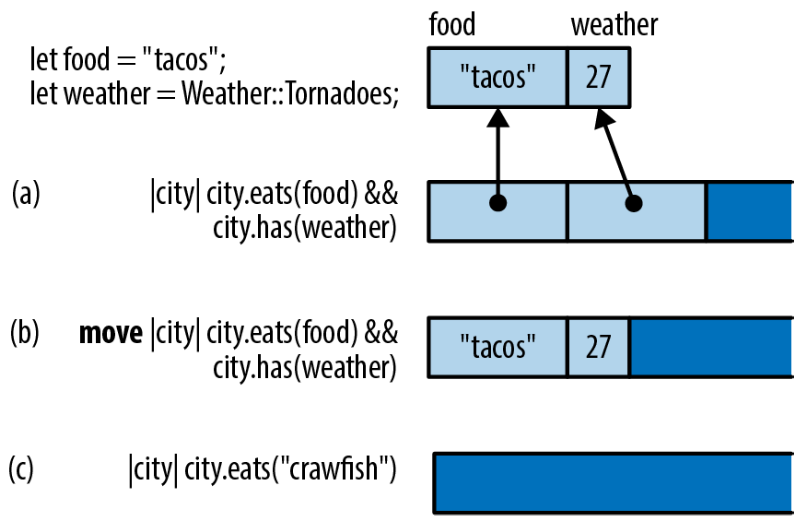
\includegraphics[width=0.9\textwidth]{../img/f14-1.png}
    \caption{必报的内存布局}
    \label{f14-1}
\end{figure}

闭包(a)使用了两个变量。显然我们在查找同时有炸玉米和龙卷放的城市。在内存中,这个闭包看起来像一个包含两个引用的结构体。

注意它并没有一个指针指向它的代码!这没有必要:只要Rust知道闭包的类型,它就知道当你调用闭包时要允许哪里的代码。

闭包(b)基本相同,除了它是一个\texttt{move}闭包,因此它包含值而不是引用。

闭包(c)并没有使用环境中的任何变量。结构体是空的,因此这个闭包不会占用任何内存。

正如图片所示,这些闭包并不会占用太多空间。但在实践中即使这一点空间有时候也不需要。通常,编译器可以把所有调用内联为一个闭包,并且即使上面的图中展示的小结构体也可能被优化掉。

在“\nameref{callback}”中,我们将展示怎么在堆上分配闭包并使用trait对象动态地调用它们。这样会稍微慢一点,但它仍然和其他的trait对象的方法一样快。

\section{闭包和安全性}

本章中到目前为止,我们已经讨论了Rust怎么保证闭包在借用或者移动环境中的值时遵循语言的安全规则。但还有更多不明显的情况。在这一节中,我们会解释当一个闭包drop或修改一个捕获的值时会发生什么。

\subsection{杀死值的闭包}
我们已经看到过借用值和偷取值的闭包,它们一路走下坡路只是时间问题。

当然,\emph{杀死(kill)}并不是真正正确的术语。在Rust中,我们\emph{丢弃(drop)}值。最直观的方法是调用\texttt{drop()}:
\begin{minted}{Rust}
    let my_str = "hello".to_string();
    let f = || drop(my_str);
\end{minted}

当调用\texttt{f}时,\texttt{my\_str}会被drop。

所以如果我们调用它两次会发生什么?
\begin{minted}{Rust}
    f();
    f();
\end{minted}

让我们深入思考它。第一次调用\texttt{f}时,它drop了\texttt{my\_str},这意味着存储字符串的内存已经被释放了,返还给了系统。第二次调用\texttt{f}时,会发生同样的事情。这是\emph{两次释放(double free)},在C++编程中这是一种会导致未定义行为的经典错误。

drop一个\texttt{String}两次在Rust中也是同样的错误行为。幸运的是,Rust不会这么简单就被骗过:
\begin{minted}{Rust}
    f();    // ok
    f();    // 错误:使用了被move的值
\end{minted}

Rust知道这个闭包不能被调用两次。

一个只能被调用一次的闭包看起来像是一个很特殊的东西,但是我们已经在整本书中都讨论过所有权和生命周期了。值被消耗(即move)的idea是Rust的核心概念之一。它在闭包中的表现和在其他情况中一样。

\subsection{\texttt{FnOnce}}
让我们再一次尝试骗过Rust、丢弃一个\texttt{String}两次。这次,我们使用这个泛型函数:
\begin{minted}{Rust}
    fn cal_twice<F>(closure: F) where F: Fn() {
        closure();
        closure();
    }
\end{minted}

这个函数可能被传入任何实现了\texttt{Fn()} trait的闭包:即没有参数并且返回\texttt{()}的闭包。(和函数一样,当返回值是\texttt{()}时可以省略;\texttt{Fn()}是\texttt{Fn() -> ()}的缩写。)

现在如果我们把我们的不安全的闭包传递给这个泛型函数会发生什么?
\begin{minted}{Rust}
    let my_str = "hello".to_string();
    let f = || drop(my_str);
    call_twice(f);
\end{minted}

这个闭包仍然在调用时drop \texttt{my\_str}。调用它两次将是两次释放。不过Rust仍然没有被迷惑:
\begin{minted}{text}
    error[E0525]: expected a closure that implements the `Fn` trait, but this closure only implements `FnOnce`
      --> closure_twice.rs:12:13
        |
      8 | let f = || drop(my_str);
        |         ^^^^^^^^______^
        |         |       |
        |         |       closure is `FnOnce` because it moves the variable `my_str`
        |         |       out of its environment
        |         this closure implements `FnOnce`, not `Fn`
      9 | call_twice(f);
        | ---------- the requirement to implement `Fn` derives from here
\end{minted}

错误信息告诉了我们更多有关Rust如何处理“杀死值的闭包”的信息。它们可以被整个语言禁用,但清理的闭包有时也是有用的。因此,Rust限制了它们的使用。drop值的闭包,例如\texttt{f},不允许实现\texttt{Fn}。它们显然完全不是\texttt{Fn}。它们实现了一个相对弱小一些的trait \texttt{FnOnce},表示只能调用一次的闭包。

当你第一次调用\texttt{FnOnce}闭包时,\emph{闭包本身会被消耗掉(the closure itself is used up)}。\texttt{Fn}和\texttt{FnOnce}这两个trait就好像是这样定义的一样:
\begin{minted}{Rust}
    // 没有参数的`Fn`和`FnOnce` trait的伪代码
    trait Fn() -> R {
        fn call(&self) -> R;
    }

    trait FnOnce() -> R {
        fn call_once(self) -> R;
    }
\end{minted}

就像算术表达式例如\texttt{a + b}是方法调用\texttt{Add::add(a, b)}的缩写一样,Rust把\texttt{closure()}看错是上面的例子中展示的两个闭包方法之一。对于一个\texttt{Fn}闭包,\texttt{closure()}会展开为\texttt{closure.call()}。这个方法以引用获取\texttt{self},因此闭包本身没有被移动。但如果闭包只有第一次调用时是安全的,那么\texttt{closure()}会展开为\texttt{closure.call\_once()}。这个方法以值获取\texttt{self}参数,因此闭包会被消耗掉。

当然,我们一直在故意使用\texttt{drop}制造麻烦。在实际中,你只会偶尔遇到这种情况。它并不会经常发生,但偶尔你会不经意间编写出消耗掉一个值的闭包代码:
\begin{minted}{Rust}
    let dict = produce_glossary();
    let debug_dump_dict = || {
        for (key, value) in dict {  // oops!
            println!("{:?} - {:?}", key, value);
        }
    };
\end{minted}

然后,当你调用\texttt{debug\_dump\_dict()}不止一次时,你会得到一个类似这样的错误信息:
\begin{minted}{text}
    error[E0382]: use of moved value: `debug_dump_dict`
      --> closures_debug_dump_dict.rs:18:5
       |
    19 |     debug_dump_dict();
       |     ----------------- `debug_dump_dict` moved due to this call
    20 |     debug_dump_dict();
       |     ^^^^^^^^^^^^^^^ value used here after move
    note: closure cannot be invoked more than once because it moves the variable
    `dict` out of its environment
      --> src/main.rs:13:29
       |
    13 |         for (key, value) in dict {
       |                             ^^^^
\end{minted}

为了调试这个错误,我们需要搞清楚为什么这个闭包是\texttt{FnOnce}。这里什么值被消耗了?编译器友好地指出了是\texttt{dict},在这个例子中,它也是我们唯一使用的变量。哦,这个bug是:我们直接迭代\texttt{dict}消耗了它。我们应该迭代\texttt{\&dict},以引用访问值,而不是迭代\texttt{dict}:
\begin{minted}{Rust}
    let debug_dump_dict = || {
        for (key, value) in &dict { // 不会消耗dict
            println!("{:?} - {:?}", key, value);
        }
    }
\end{minted}

这样就修复了错误;这个函数现在是\texttt{Fn},可以被调用任意次。

\subsection{\texttt{FnMut}}
还有一种闭包,这种闭包包含可变的数据或者\texttt{mut}引用。

Rust认为non-\texttt{mut}的值可以安全在线程间共享。但在线程间共享这种包含\texttt{mut}数据的non-\texttt{mut}闭包不是安全的:在多个线程中调用这种闭包可能会导致各种数据竞争,就和多个线程同时读写同一份数据一样。

因此,Rust又分出了一种闭包类别\texttt{FnMut},这个类别用于有写入操作的闭包。\texttt{FnMut}闭包以\texttt{mut}引用调用,就好像它们被定义为这样:
\begin{minted}{Rust}
    // `Fn`, `FnMut`, `FnOnce` trait的伪代码。
    trait Fn() -> R {
        fn call(&self) -> R;
    }

    trait FnMut() -> R {
        fn call_mut(&mut self) -> R;
    }

    trait FnOnce() -> R {
        fn call_once(self) -> R;
    }
\end{minted}

所有需要值的\texttt{mut}方法,但不会drop任何值的闭包,都是一个\texttt{FnMut}闭包。例如:
\begin{minted}{Rust}
    let mut i = 0;
    let incr = || {
        i += 1; // incr借用了i的一个可变引用
        println!("Ding! i is now: {}", i);
    };
    call_twice(incr);
\end{minted}

我们编写的\texttt{call\_twice}需要一个\texttt{Fn}。因为\texttt{incr}是一个\texttt{FnMut}而不是\texttt{Fn},所以这段代码回编译失败。然而,有一种简单的修复方法。为了理解这种修复方法,让我们后退一步,总结一下你学到的有关Rust的三种闭包的知识:
\begin{itemize}
    \item \texttt{Fn}是你可以没有限制地调用多次的闭包和函数家族。这个最高的类别还包括所有的\texttt{fn}函数。
    \item \texttt{FnMut}是如果闭包本身被声明为\texttt{mut}时可以调用多次的闭包家族。
    \item \texttt{FnOnce}是当调用者拥有它时可以调用一次的闭包家族。
\end{itemize}

每一个\texttt{Fn}都满足\texttt{FnMut}的要求,每一个\texttt{FnMut}都满足\texttt{FnOnce}的要求。如\autoref{f14-2}所示,它们并不是独立的三个类别。

\texttt{Fn()}是\texttt{FnMut()}的一个子集,\texttt{FnMut()}又是\texttt{FnOnce()}的一个子集。这使得\texttt{Fn}是最独特和强大的分类。\texttt{FnMut}和\texttt{FnOnce}是范围更广一些的分类,它们包含有一些使用限制的闭包。

\begin{figure}[htbp]
    \centering
    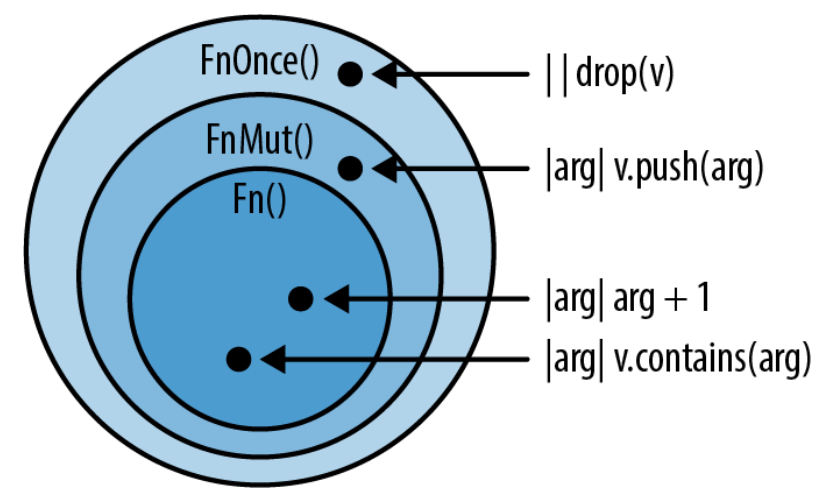
\includegraphics[width=0.9\textwidth]{../img/f14-2.png}
    \caption{三种闭包类别的维恩图}
    \label{f14-2}
\end{figure}

现在我们已经梳理了我们所知的内容,显然为了尽可能接受更多的闭包类型,我们的\texttt{call\_twice}实际上应该接受所有的\texttt{FnMut}闭包,像这样:
\begin{minted}{Rust}
    fn call_twice<F>(mut closure: F) where F: FnMut() {
        closure();
        closure();
    }
\end{minted}

原本第一行的约束是\texttt{F: Fn()},现在是\texttt{F: FnMut()}。有了这个修改之后,我们仍然可以接受所有的\texttt{Fn}闭包,并且现在还可以对可变的数据调用调用\texttt{call\_twice}:
\begin{minted}{Rust}
    let mut i = 0;
    call_twice(|| i += 1);  // ok!
    assert_eq!(i, 2);
\end{minted}

\subsection{闭包的\texttt{Copy}和\texttt{Clone}}
正如Rust能自动分辨出哪些闭包只能调用一次一样,它也能分辨出哪些闭包可以实现\texttt{Copy}和\texttt{Clone},哪些不能。

正如我们之前解释的一样,闭包被表示为包含它们捕获的值(\texttt{move}闭包)或者引用(non-\texttt{move}闭包)的结构体。闭包的\texttt{Copy}和\texttt{Clone}的规则就类似于普通结构体的\texttt{Copy}和\texttt{Clone}的规则。一个没有可变变量的non-\texttt{move}的闭包只有共享引用,共享引用是\texttt{Clone}和\texttt{Copy},所以这种闭包也是\texttt{Clone}和\texttt{Copy}:
\begin{minted}{Rust}
    let y = 10;
    let add_y = |x| x + y;
    let copy_of_add_y = add_y;                  // 这个闭包是`Copy`,因此...
    assert_eq!(add_y(copy_of_add_y(22)), 42);   // ...我们可以使用这两个。
\end{minted}

另一方面,一个\emph{有}可变值的non-\texttt{move}闭包在内部的表示中包含可变引用。可变引用既不是\texttt{Clone}也不是\texttt{Copy},因此这样的一个闭包既不是\texttt{Copy}也不是\texttt{Clone}:
\begin{minted}{Rust}
    let mut x = 0;
    let mut add_to_x = |n| { x += n; x };

    let copy_of_add_to_x = add_to_x;                // 移动,而不是拷贝
    assert_eq!(add_to_x(copy_of_add_to_x(1)), 2);   // 错误:使用了被移动的值
\end{minted}

对于\texttt{move}闭包来说,规则变得更简单了。如果一个\texttt{move}闭包捕获的所有值都是\texttt{Copy},那么它也是\texttt{Copy}。如果它捕获的所有值都是\texttt{Clone},那么它也是\texttt{Clone}。例如:
\begin{minted}{Rust}
    let mut greeting = String::from("Hello, ");
    let greet = move |name| {
        greeting.push_str(name);
        println!("{}", greeting);
    };
    greet.clone()("Alfred");
    greet.clone()("Bruce");
\end{minted}

这个\texttt{.clone()(...)}语法有一点奇怪,但它只是因为着我们克隆了闭包然后调用它。这个程序输出:
\begin{minted}{Rust}
    Hello, Alfred
    Hello, Bruce
\end{minted}

当\texttt{greeting}在\texttt{greet}中使用时,它会被移动进表示\texttt{greet}的内部结构体里,因为它是\texttt{move}闭包。因此,当我们克隆\texttt{greet}时,它里面的所有内容都会被克隆。这里有两个\texttt{greeting}的拷贝,当调用克隆的\texttt{greet}时它们会被独立地修改。它本身用处不大,但当你需要把同样的闭包传递给不止一个函数时,它会很有用。

\section{回调}\label{callback}

很多库使用\emph{回调(callback)}作为部分API:一种由用户提供、之后会被库调用的函数。事实上,你已经在这本书中看到过一些这样的API了。回顾\hyperref[ch02]{第2章},我们使用了\texttt{actix-web}框架编写了一个简单的web服务器。程序中很重要的一部分就是路由,看起来像这样:
\begin{minted}{Rust}
    App::new()
        .route("/", web::get().to(get_index))
        .route("/gcd", web::post().to(post_gcd))
\end{minted}

路由的目的是把到来的网络请求发送到处理特定种类请求的函数。在这个例子中,\texttt{get\_index}和\texttt{post\_gcd}是我们在程序里其他地方用\texttt{fn}关键字声明的函数的名字,但我们也可以传递一个闭包,像这样:
\begin{minted}{Rust}
    App::new()
        .route("/", web::get().to(|| {
            HttpResponse::Ok()
                .content_type("text/html")
                .body("<title>GCD Calculator</title>...")
        }))
        .route("/gcd", web::post().to(|form: web::Form<GcdParameters>| {
            HttpResponse::Ok()
                .content_type("text/html")
                .body(format!("The GCD of {} and {} is {}.",
                              form.n, form.m, gcd(form.n, form.m)))
        }))
\end{minted}

这是因为\texttt{actix-web}被设计为可以接受任何线程安全的\texttt{Fn}作为参数。

那么我们怎么在自己的程序中做到这一点呢?让我们尝试写出我们自己的简单的路由,不使用任何\texttt{actix-web}的代码。我们首先声明一些表示HTTP请求和响应的类型:
\begin{minted}{Rust}
    struct Request {
        method: String,
        url: String,
        headers: HashMap<String, String>
        body: Vec<u8>
    }

    struct Response {
        code: u32,
        headers: HashMap<String, String>
        body: Vec<u8>
    }
\end{minted}

现在一个路由器的任务就是简单地存储一个把URL映射到回调函数的表,这样可以按需调用正确的回调函数。(为了简单起见,我们只允许用户创建匹配单个确切的URL。)

\begin{minted}{Rust}
    struct BasicRouter<C> where C: Fn(&Request) -> Response {
        routes: HashMap<String, C>
    }

    impl<C> BasicRouter<C> where C: Fn(&Request) -> Response {
        /// 创建一个空的路由器。
        fn new() -> BasicRouter<C> {
            BasicRouter { routes: HashMap::new() }
        }

        /// 向路由器中添加一条路由。
        fn add_route(&mut self, url: &str, callback: C) {
            self.routes.insert(url.to_string(), callback);
        }
    }
\end{minted}

不幸的是,我们犯了一个错误。你注意到它了吗?

如果我们只添加一个路由,那么这个路由器可以工作的很好:
\begin{minted}{Rust}
    let mut router = BasicRouter::new();
    router.add_route("/", |_| get_form_response());
\end{minted}

这可以正常编译并运行。然而,如果我们添加另一个路由:
\begin{minted}{Rust}
    router.add_route("/gcd", |req| get_gcd_response(req));
\end{minted}

那我们会得到错误:
\begin{minted}{text}
    error[E0308]: mismatched types
      --> closures_bad_router.rs:41:30
       |
    41 |     router.add_route("/gcd", |req| get_gcd_response(req));
       |                              ^^^^^^^^^^^^^^^^^^^^^^^^^^^
       |                              expected closure, found a different closure
       |
       = note: expected type `[closure@closures_bad_router.rs:40:27: 40:50]`
                  found type `[closure@closures_bad_router.rs:41:30: 41:57]`
    note: no two closures, even if identical, have the same type
    help: consider boxing your closure and/or using it as a trait object
\end{minted}

我们的错误在于定义\texttt{BasicRouter}类型的方式:
\begin{minted}{Rust}
    struct BasicRouter<C> where C: Fn(&Request) -> Response {
        routes: HashMap<String, C>
    }
\end{minted}

我们不知不觉中声明了每一个\texttt{BasicRouter}都有单一的回调类型\texttt{C},并且\texttt{HashMap}里的所有回调函数都是这个类型。回顾“\nameref{WhichToUse}”,我们展示了一个有同样问题的\texttt{Salad}类型:
\begin{minted}{Rust}
    struct Salad<V: Vegetable> {
        veggies: Vec<V>
    }
\end{minted}
这里的解决方法和沙拉问题的解决方法一样:因为我们想支持很多类型,我们需要使用box和trait对象:
\begin{minted}{Rust}
    type BoxedCallback = Box<dyn Fn(&Request) -> Response>;

    struct BasicRouter {
        routes: HashMap<String, BoxedCallback>
    }
\end{minted}

每一个box都可以包含一个不同类型的闭包,因此一个\texttt{HashMap}可以包含很多种类的回调函数。注意类型参数\texttt{C}消失了。

这需要对方法进行一些调整:
\begin{minted}{Rust}
    impl BasicRouter {
        // 创建一个空的路由器。
        fn new() -> BasicRouter {
            BasicRouter { routes: HashMap::new() }
        }

        // 向路由器中添加一条路由。
        fn add_route<C>(&mut self, url: &str, callback: C)
            where C: Fn(&Request) -> Response + 'static
        {
            self.routes.insert(url.to_string(), Box::new(callback));
        }
    }
\end{minted}

\begin{note}
    注意\texttt{add\_route}的类型签名中\texttt{C}的两个约束:一个特定的\texttt{Fn} trait和一个\texttt{'static}生命周期。Rust让我们添加这个\texttt{'static}约束。如果没有它,\texttt{Box::new(callback)}的调用将会导致错误,因为如果一个闭包包含可能会离开作用域的变量的引用,那么存储这样的闭包是不安全的。
\end{note}

最后,我们的简单路由已经准备好处理到来的请求:
\begin{minted}{Rust}
    impl BasicRouter {
        fn handle_request(&self, request: &Request) -> Response {
            match self.routes.get(&request.url) {
                None => not_found_response(),
                Some(callback) => callback(request)
            }
        }
    }
\end{minted}

作为灵活性的代价,我们也可以使用\emph{函数指针(function pointer)}或者\texttt{fn}类型来代替trait对象,这样空间效率会高一点。像\texttt{fn(u32) -> u32}这样的类型,和闭包很像:
\begin{minted}{Rust}
    fn add_ten(x: u32) -> u32 {
        x + 10
    }

    let fn_ptr: fn(u32) -> u32 = add_ten;
    let eleven = fn_ptr(1); // 11
\end{minted}

事实上,不捕获环境中任何变量的闭包和函数指针完全相同,因为它们不需要存储关于被捕获变量的额外信息。如果你指定了合适的\texttt{fn}类型,不管是在绑定中还是在函数签名中,编译器都会乐于让你使用它们:
\begin{minted}{Rust}
    let closure_ptr: fn(u32) -> u32 = |x| x + 1;
    let two = closure_ptr(1);   // 2
\end{minted}

与那些捕获的闭包不同,这些函数指针只占据一个\texttt{usize}的空间。

函数指针也可以用于实现我们自己的动态分发,而不是使用编译器建议的\texttt{Box dyn Fn()}:
\begin{minted}{Rust}
    struct FnPointerRouter {
        routes: HashMap<String, fn(&Request) -> Response>
    }
\end{minted}

这里,\texttt{HashMap}只为每一个\texttt{String}存储一个\texttt{usize},这里没有\texttt{Box}。除了\texttt{HashMap}自身,没有任何动态分配。当然,这些方法也需要被调整:
\begin{minted}{Rust}
    impl FnPointerRouter {
        // 创建一个空的路由器。
        fn new() -> FnPointerRouter {
            FnPointerRouter { routes: HashMap::new() }
        }

        // 向路由器中添加一条路由。
        fn add_route(&mut self, url: &str, callback: fn(&Request) -> Response)
        {
            self.routes.insert(url.to_string(), callback);
        }
    }
\end{minted}

如\autoref{f14-1}所示,闭包会有单独的类型是因为每一个闭包都捕获了不同的变量,因此它们每一个的大小都不同。如果它们不捕获任何内容,就没有任何东西需要存储。在接受回调的函数中使用\texttt{fn}指针,可以限制调用只能使用没有捕获东西的闭包,这样在代码内能获取一些性能和灵活性的改善,但对于使用你的API的用户来说要付出灵活性的代价。

\section{高效地使用闭包}



    \chapter{迭代器}\label{ch15}

\emph{It was the end of a very long day.}

\begin{flushright}
    ——Phil
\end{flushright}

一个\emph{迭代器(iterator)}可以产生一个指的序列,通常会使用一个循环来进行处理。Rust的标准库提供了遍历vector、字符串、哈希表和其他集合的迭代器,以及从一个输入流中产生若干行文本的迭代器、到达网络服务器的连接的迭代器、通过通道从其他线程接收到的值的迭代器,等等。当然,你可以实现自己的迭代器。Rust的\texttt{for}循环提供了一种自然地使用迭代器的语法,但迭代器自身也提供了丰富的方法集合用于映射、过滤、连接、收集等用途。

Rust的迭代器灵活、表达力强、高效。考虑下面的函数,它返回前\texttt{n}个正数的和(通常也被称为\emph{第n个三角数(nth triangle number)}:
\begin{minted}{Rust}
    fn triangle(n: i32) -> i32 {
        let mut sum = 0;
        for i in 1..=n {
            sum += i;
        }
        sum
    }
\end{minted}

表达式\texttt{1..=n}是一个\texttt{RangeInclusive<i32>}值。一个\texttt{RangeInclusive<i32>}是一个产生从起点到终点的所有整数的迭代器(包含起点和终点),因此你可以将它用作\texttt{for}循环的操作数来求\texttt{1}到\texttt{n}的和。

但迭代器也有一个\texttt{fold}方法,你可以使用它实现如下的等价定义:
\begin{minted}{Rust}
    fn triangle(n: i32) -> i32 {
        (1..=n).fold(0, |sum, item| sum + item)
    }
\end{minted}

以\texttt{0}作为起始的总和,\texttt{fold}会获取\texttt{1..=n}产生的每个值,然后用总和和产生的值调用闭包\texttt{|sum, item| sum + item},每一次闭包的返回值就是新的总和。它最后返回的值就是\texttt{fold}自身返回的值——在这个例子中,就是整个序列的总和。如果你习惯使用\texttt{for}和\texttt{while}循环,那么这看起来会有些奇怪,但一旦你习惯了它,\texttt{fold}就是一个可读性强而简洁的替代方案。

这种写法是函数式编程语言的标准写法,这使得表达式有更强的表现力。但Rsut的迭代器是精心设计的,为了保证编译器可以把它们翻译成优秀的机器代码。在release构建模式下构建上面第二个定义时,Rust知道\texttt{fold}的定义,并且把它内联进\texttt{triangle}。然后,闭包\texttt{|sum, item| sum + item}也会被内联。最后,Rust会检查组合之后的代码,然后发现有一种更简单的方法计算从1到\texttt{n}的和:和总是等于\texttt{n * (n+1) / 2}。Rust会把\texttt{triangle}的整个函数体,包括循环、闭包等所有内容,变成一次乘法指令和一些其他的位运算。

这个例子恰巧可以转换成简单的算术,但在更复杂的使用中迭代器也可以表现的很好。它们是Rust提供灵活抽象的同时只有很小甚至没有开销的另一个例子。

在本章中,我们将会解释:
\begin{itemize}
    \item \texttt{Iterator}和\texttt{IntoIterator} trait,它们是Rust迭代器的基础
    \item 经典迭代器管道的三个阶段:从初始的值创建一个迭代器;通过选择或处理值将一种迭代器变成另一种;消耗迭代器产生的值
    \item 如何为自己的类型实现迭代器
\end{itemize}

迭代器有很多方法,所以一旦你了解了大概的思路,就可以跳过一节。但迭代器在Rust的习惯用法中非常普遍,熟悉这些随附的工具对掌握这门语言至关重要。

\section{\texttt{Iterator}与\texttt{IntoIterator trait}}\label{iter}

一个迭代器是任何实现了\texttt{std::iter::Iterator} trait的类型:
\begin{minted}{Rust}
    trait Iterator {
        type Item;
        fn next(&mut self) -> Option<Self::Item>;
        ... // 很多默认方法
    }
\end{minted}

\texttt{Item}是迭代器产生的值的类型。\texttt{next}方法可能返回\texttt{Some(v)},其中\texttt{v}是迭代器的下一个值;或者返回\texttt{None},表示已经到达序列的终点。这里我们省略了\texttt{Iterator}的很多默认方法;我们将在本章的剩余部分分别介绍它们。

如果有一种自然的方法从一个类型上迭代,那么这个类型可以实现\texttt{std::iter::IntoIterator},它的\texttt{into\_iter}方法获取一个值并返回一个迭代它的迭代器:
\begin{minted}{Rust}
    trait IntoIterator where Self::IntoIter: Iterator<Item=Self::Item> {
        type Item;
        type IntoIter: Iterator;
        fn into_iter(self) -> Self::IntoIter;
    }
\end{minted}

\texttt{IntoIter}是迭代器自身的类型,\texttt{Item}是它产生的值的类型。我们称所有实现了\texttt{IntoIterator}的类型为\emph{可迭代对象(iterable)},因为你可以迭代它。

Rust的\texttt{for}循环将这些部分漂亮地组合在一起。为了迭代一个迭代器的元素,你可以写:
\begin{minted}{Rust}
    println!("There's:");
    let v = vec!["antimony", "arsenic", "alumium", "selenium"];

    for element in &v {
        println!("{}", element);
    }
\end{minted}

在底层,每一个\texttt{for}循环只是\texttt{IntoIterator}和\texttt{Iterator}的方法调用的缩写:
\begin{minted}{Rust}
    let mut iterator = (&v).into_iter();
    while let Some(element) = iterator.next() {
        println!("{}", element);
    }
\end{minted}

\texttt{for}循环使用了\texttt{IntoIterator::into\_iter}来把操作数\texttt{\&v}转换成一个迭代器,然后重复调用\texttt{Iterator::next}。每一次返回\texttt{Some(element)}时,\texttt{for}循环会执行循环体;如果它返回\texttt{None},循环会终止。

考虑这个例子,其中有一些迭代器的术语:
\begin{itemize}
    \item 正如我们所说,\emph{迭代器(iterator)}是任何实现了\texttt{Iterator}的类型。
    \item \emph{可迭代对象(iterable)}是任何实现了\texttt{IntoIterator}的类型:你可以通过调用它的\texttt{into\_iter}方法获得一个迭代它的迭代器。这个例子中vector的引用\texttt{\&v}就是可迭代对象。
    \item 一个迭代器\emph{产生(produce)}值。
    \item 迭代器产生的值是\emph{item}。这里,item是\texttt{"antimony", "arsenic},等等。
    \item 接受迭代器产生的item的代码是\emph{消费者(consumer)}。这个例子中,\texttt{for}循环就是消费者。
\end{itemize}

尽管\texttt{for}循环总是调用操作数的\texttt{into\_iter},你也可以直接向\texttt{for}循环传递迭代器;例如,当你在\texttt{Range}上循环时就是这种情况。所有的迭代器都会自动实现\texttt{IntoIterator},它们的\texttt{into\_iter}方法简单地返回迭代器自身。

如果在迭代器返回了\texttt{None}之后,你再调用它的\texttt{next}方法,那么\texttt{Iterator} trait并没有指定这种情况下该怎么做。大多数会再次返回\texttt{None},但不是所有。(如果这导致了问题,“\nameref{fuse}”中介绍的\texttt{fuse}适配器可能会有帮助。)

\section{创建迭代器}
Rust标准库文档中详细解释了每种类型提供哪些种类的迭代器,但标准库提供了一些通用的约定来帮助你找到需要的迭代器。

\subsection{\texttt{iter}和\texttt{iter\_mut}方法}
大多数集合类型提供\texttt{iter}和\texttt{iter\_mut}方法,它们返回一个迭代器,迭代器会产生每一个item的共享引用或可变引用。数组切片例如\texttt{\&[T]}和\texttt{\&mut [T]}也有\texttt{iter}和\texttt{iter\_mut}方法。除了使用\texttt{for}循环自动处理之外,这些方法是最常用的获得迭代器的方法:
\begin{minted}{Rust}
    let v = vec![4, 20, 12, 8, 6];
    let mut iterator = v.iter();
    assert_eq!(iterator.next(), Some(&4));
    assert_eq!(iterator.next(), Some(&20));
    assert_eq!(iterator.next(), Some(&12));
    assert_eq!(iterator.next(), Some(&8));
    assert_eq!(iterator.next(), Some(&6));
    assert_eq!(iterator.next(), None);
\end{minted}

这个迭代器的item类型是\texttt{\&i32}:每一次调用\texttt{next}都会产生下一个元素的引用,直到到达vector的终点。

每一个类型都可以实现\texttt{iter}和\texttt{iter\_mut},不管它们实现的方式是什么。\texttt{std::path::Path}的\texttt{iter}返回的迭代器一次产生路径的一段:
\begin{minted}{Rust}
    use std::ffi::OsStr;
    use std::path::Path;

    let path = Path::new("C:/Users/JimB/Downloads/Fedora.iso");
    let mut iterator = path.iter();
    assert_eq!(iterator.next(), Some(OsStr::new("C:")));
    assert_eq!(iterator.next(), Some(OsStr::new("Users")));
    assert_eq!(iterator.next(), Some(OsStr::new("JimB")));
    ...
\end{minted}

这个迭代器的item类型是\texttt{\&std::ffi::OsStr},它是操作系统调用接受的一种字符串类型的引用切片。

如果某个类型有不止一种迭代方式,那么这个类型通常为每种遍历方式提供特定的方法,因为这时普通的\texttt{iter}方法将会导致歧义。例如,\texttt{\&str}字符串切片类型没有\texttt{iter}方法。作为替代,假设\texttt{s}是\texttt{\&str},那么\texttt{s.bytes()}返回一个产生\texttt{s}的每个字节的迭代器,而\texttt{s.chars()}会以UTF-8编码解析它的内容,然后产生每一个Unicode字符。

\subsection{\texttt{IntoIterator}实现}
当一个类型实现了\texttt{IntoIterator}之后,你可以自己调用它的\texttt{into\_iter}方法,正如\texttt{for}循环做的一样:
\begin{minted}{Rust}
    // 你通常应该使用HashSet,但它的迭代顺序是不确定的,
    // 因此这个例子中BTreeSet会工作得更好。
    use std::collections::BTreeSet;
    let mut favorites = BTreeSet::new();
    favorites.insert("Lucy in the Sky With Diamonds".to_string());
    favorites.insert("Liebesträume No. 3".to_string());

    let mut it = favorites.into_iter();
    assert_eq!(it.next(), Some("Liebesträume No. 3".to_string()));
    assert_eq!(it.next(), Some("Lucy in the Sky With Diamonds".to_string()));
    assert_eq!(it.next(), None);
\end{minted}

大多数集合实际上都提供了好几个\texttt{IntoIterator}的实现,分别是为共享引用(\texttt{\&T})、可变引用(\texttt{\&mut T})、移动(\texttt{T})提供的实现:
\begin{itemize}
    \item 给定一个集合的\emph{共享引用(shared reference)},\texttt{into\_iter}返回一个产生item的共享引用的迭代器。例如,在上面的代码中,\texttt{(\&favorites).into\_iter()}将会返回一个\texttt{Item}类型是\texttt{\&String}的迭代器。
    \item 给定一个集合的\emph{可变引用(mutable reference)},\texttt{into\_iter}返回一个产生item的可变引用的迭代器。例如,如果\texttt{vector}是\texttt{Vec<String>},那么\texttt{(\&mut vector).into\_iter()}将返回一个\texttt{Item}类型是\texttt{\&mut String}的迭代器。
    \item 当集合\emph{以值}传递时,\texttt{into\_iter}返回一个获取集合所有权并返回item自身的迭代器;item的所有权从集合移动到消费者,原来的集合在这个过程中被消耗。例如,上面代码中的\texttt{favorites.into\_iter()}会返回一个产生每个字符串值的迭代器;消费者会接受每个字符串的所有权。当迭代器被drop时,\texttt{BTreeSet}中剩余的所有元素也都会被drop,并且集合会变为未初始化。
\end{itemize}

因为一个\texttt{for}循环会对操作数调用\texttt{IntoIterator::into\_iter},这三种实现会导致有下面三种迭代方式:迭代集合的共享引用、迭代集合的可变引用、或者消耗集合并获取它的元素的所有权:
\begin{minted}{Rust}
    for element in &collection { ... }
    for element in &mut collection { ... }
    for element in collection { ... }
\end{minted}

这三种写法会调用上面列出的\texttt{IntoIterator}实现之一。

并不是每个类型都提供了全部这三种实现。例如,\texttt{HashSet}、\texttt{BTreeSet}、\texttt{BinaryHeap}没有实现共享引用的\texttt{IntoIterator},因为修改它们的元素可能会破坏类型的不变量:修改后的值可能会有不同的哈希值、或者和它的邻居的顺序关系会改变,因此修改元素会导致它们北方在错误的地方。其他的类型支持可变性,但只支持部分。例如,\texttt{HashMap}和\texttt{BTreeMap}产生表项的value的可变引用,以及key的共享引用,原因和上面类似。

一般的准则是迭代应该高效和可预测,因此Rust不提供开销很大或者可能展现出令人惊讶的行为的实现(例如,重新哈希被修改的\texttt{HashSet}条目并因此导致之后的迭代中可能再次遇到它们)。

切片实现了三种\texttt{IntoIterator}变体中的两个;因为它们并不拥有自己引用的元素,因此没有“以值”的实现。作为代替,\texttt{\&[T]}和\texttt{\&mut [T]}的\texttt{into\_iter}返回一个产生共享引用和可变引用的迭代器。如果你把底层切片类型\texttt{[T]}想象成一种集合,那么它就落入了之前的模式。

你可能已经注意到前两种\texttt{IntoIterator}的变体产生共享和可变的引用,这和调用\texttt{iter}或者\texttt{iter\_mut}是等价的。为什么Rust同时提供两者?

\texttt{IntoIterator}让\texttt{for}循环能正常工作,因此它显然是必要的。但当你不使用\texttt{for}循环时,使用\texttt{favorites.iter()}比\texttt{(\&favorites).into\_iter()}更加清晰。你可能会频繁需要以共享引用迭代,因此\texttt{iter}和\texttt{iter\_mut}也很有用。

\texttt{IntoIterator}在泛型代码中也很有用:你可以使用一个约束例如\texttt{T: IntoIterator}来限制类型参数\texttt{T}必须是可以迭代的类型。或者,你可以写\texttt{T: IntoIterator<Item=U>}来进一步要求迭代会产生\texttt{U}类型的值。例如,这个函数打印出任何item可以用\texttt{"{:?}"}格式打印的可迭代对象:
\begin{minted}{Rust}
    use std::fmt::Debug;

    fn dump<T, U>(t: T)
        where T: IntoIterator<Item=U>,
              U: Debug
    {
        for u in t {
            println!("{:?}", u);
        }
    }
\end{minted}
你不能在这个泛型函数中使用\texttt{iter}或者\texttt{iter\_mut},因为它们不是任何trait的方法:大多数可迭代类型只是恰好有这两个方法。

\subsection{\texttt{from\_fn}和\texttt{successors}}

一个简单而通用的产生一个值序列的方式是提供一个返回它们的闭包。

给定一个返回\texttt{Option<T>}的函数,\texttt{std::iter::from\_fn}返回一个迭代器,它简单地调用那个函数来产生item。例如:
\begin{minted}{Rust}
    use rand::random;   // 在Cargo.toml中添加依赖:rand = "0.7"
    use std::iter::from_fn;
    // 产生1000个随机数,在[0, 1]之间均匀分布。
    // (这并不是你想在`rand_distr` crate中找到的分布,
    // 但你可以很容易地自己实现它)
    let lengths: Vec<f64> =
        from_fn(|| Some((random::<f64>() - random::<f64>()).abs()))
        .take(1000)
        .collect();
\end{minted}

这里调用了\texttt{from\_fn}来制作一个产生随机数的迭代器。因为这个迭代器总是返回\texttt{Some},因此这个序列永远不会终止,但我们调用了\texttt{take(1000)}来限制只要前1000个元素。然后\texttt{collect}从最后的迭代器构建一个vector。这是一种高效地构建初始化的vector的方式。我们将在本章稍后的“\nameref{BuildColl}”中介绍为什么。

如果每一个item都依赖上一个,那么\texttt{std::iter::successors}函数可以漂亮地工作。你需要提供一个初始item,和一个获取上一个item并返回一个下一个item的\texttt{Option}。如果返回\texttt{None},那么迭代终止。例如,这里有另一种编写\hyperref[ch02]{第2章}中的曼德勃罗集绘制器的\texttt{escape\_time}函数的方法:
\begin{minted}{Rust}
    use num::Complex;
    use std::iter::successors;

    fn escape_time(c: Complex<f64>, limit: usize) -> Option<usize> {
        let zero = Complex { re: 0.0, im: 0.0 };
        successors(Some(zero), |&z| { Some(z * z + c) })
            .take(limit)
            .enumerate()
            .find(|(_i, z)| z.norm_sqr() > 4.0)
            .map(|(i, _z)| i)
    }
\end{minted}

从zero开始,\texttt{successors}调用通过重复平方再加上参数\texttt{c}来产生一个复平面上点的序列。当绘制曼德勃罗集时,我们希望知道这个序列会一直在原点附近还是远离原点。\texttt{take(limit)}调用设置了序列长度的限制,\texttt{enumerate}为每一个点加上一个序号、把每个点\texttt{z}变为元组\texttt{(i, z)}。然后我们使用\texttt{find}来查找第一个离远点足够远可以逃离的点。如果存在这样的点,\texttt{find}方法返回一个\texttt{Option::Some((i, z))},否则返回\texttt{None}。\texttt{Option::map}的调用会把\texttt{Some((i, z))}变为\texttt{Some(i)},但不会改变\texttt{None}:这正是我们想要的返回值。

\texttt{from\_fn}和\texttt{successors}都接受\texttt{FnMut}闭包,因此你的闭包可以捕获并修改作用域中的变量。例如,这个\texttt{fibonacci}函数使用一个\texttt{move}闭包来捕获一个变量并使用它作为运行状态:
\begin{minted}{Rust}
    fn fibonacci() -> impl Iterator<Item=usize> {
        let mut state = (0, 1);
        std::iter::from_fn(move || {
            state = (state.1, state.0 + state.1);
            Some(state.0)
        })
    }

    assert_eq!(fibonacci().take(8).collect::<Vec<_>>(),
               vec![1, 1, 2, 3, 5, 8, 13, 21]);
\end{minted}

注意:\texttt{from\_fn}和\texttt{successors}方法非常灵活,你可以通过传递闭包来达到你想要的行为,并将很多迭代器的使用变为一次对其中一个的调用。但这样做会忽略迭代器提供的表明数据流动和使用标准名称用于通用模式的能力。在你使用这两个函数之前请确保你已经熟悉了本章中的其他迭代器方法,它们通常是更好的完成工的方式。

\subsection{\texttt{drain}方法}
很多集合类型提供一个\texttt{drain}方法来获取集合的可变引用,并返回一个迭代器把每个元素的所有权传递给消费者。然而,和\texttt{into\_iter()}以值获取集合并消耗它不同,\texttt{drain}借用一个集合的可变引用,并且当迭代器被drop时,它会移除集合中剩余的所有元素,让集合变为空。

对于可以用范围索引的类型,例如\texttt{String}、vector、\texttt{VecDeque},\texttt{drain}方法获取一个要移除的元素的范围,而不是消耗整个序列:
\begin{minted}{Rust}
    use std::iter::FromIterator;

    let mut outer = "Earth".to_string();
    let inner = String::from_iter(outer.dran(1..4));

    assert_eq!(outer, "Eh");
    assert_eq!(inner, "art");
\end{minted}

如果你确实要消耗整个序列,使用整个范围\texttt{..}作为参数。

\subsection{其他迭代器源}
上面的几节基本都是关于像vector和\texttt{HashMap}这样的集合类型的,但标准库中还有很多其他类型支持迭代。\autoref{t15-1}总结了一些有趣的类型,但还有更多没有列出。我们将在专门介绍特定类型的章节(即\hyperref[ch16]{第16章}、\hyperref[ch17]{第17章}、\hyperref[ch18]{第18章})中详细介绍其中的一些方法。

\begin{longtable}{p{0.22\textwidth}p{0.23\textwidth}p{0.45\textwidth}}
    \caption{标准库中的其他迭代器}
    \label{t15-1}\\
    \hline
    \textbf{类型或trait} & \textbf{表达式} & \textbf{注意} \\
    \hline
    \multirow{2}{*}{\texttt{std::ops::Range}} & \texttt{1..10} & 端点必须是整数才能迭代。包括起点但不包括终点。 \\
    & \texttt{(1..10).step\_by(2)} \cellcolor{tablecolor} & 产生1,3,5,7,9。 \cellcolor{tablecolor} \\
    \hline
    \texttt{std::ops::RangeFrom} & \texttt{1..} & 无限迭代。起点必须是整数。当值到达了这种类型的极限时可能会panic或者溢出。 \\
    \hline
    \rowcolor{tablecolor}
    \texttt{std::ops:: RangeInclusive} & \texttt{1..=10} & 类似\texttt{Range},但包括终点值。 \\
    \hline
    \texttt{Option<T>} & \texttt{Some(10).iter()} & 类似于一个长度为0(\texttt{None})或1的vector(\texttt{Some(v)})。 \\
    \hline
    \rowcolor{tablecolor}
    \texttt{Result<T, E>} & \texttt{Ok("blah").iter()} & 类似于\texttt{Option},产生\texttt{Ok}值。 \\
    \hline
    \multirow{7}{*}{\texttt{Vec<T>, \&[T]}} & \texttt{v.windows(16)} & 从左到右产生重叠的、连续的给定长度的切片。 \\
    & \texttt{v.chunks(16)} \cellcolor{tablecolor} & 从左到右产生非重叠的、连续的给定长度的切片。 \cellcolor{tablecolor} \\
    & \texttt{v.chunks\_mut(1024)} & 类似\texttt{chunks},不过切片是可变的。 \\
    & \texttt{v.split(|byte| byte \& 1 != 0)} \cellcolor{tablecolor} & 产生被满足条件的元素分隔的切片。 \cellcolor{tablecolor} \\
    & \texttt{v.split\_mut(...)} & 同上,但产生可变切片。 \\
    & \texttt{v.rsplit(...)} \cellcolor{tablecolor} & 类似\texttt{split},但从右向左产生切片。 \cellcolor{tablecolor} \\
    & \texttt{v.splitn(n, ...)} & 类似\texttt{split},但最多产生\texttt{n}个切片。 \\
    \hline
    \multirow{5}{*}{\texttt{String, \&str}} & \texttt{s.bytes()} \cellcolor{tablecolor} & 产生UTF-8字符串的字节。 \cellcolor{tablecolor} \\
    & \texttt{s.chars()} & 产生UTF-8字符串的\texttt{char}。 \\
    & \texttt{s.split\_whitespace()} \cellcolor{tablecolor} & 以空格分隔字符串,产生非空字符们的切片。 \cellcolor{tablecolor} \\
    & \texttt{s.lines()} & 产生字符串的每一行的切片。 \\
    & \texttt{s.split('/')} \cellcolor{tablecolor} & 用给定的模式分隔字符串,产生每两个匹配之间的内容的切片。模式可以是字符、字符串或者闭包。\cellcolor    {tablecolor} \\
    \hline
    \multirow{5}{*}{\shortstack[l]{\texttt{std::collections::}\\\texttt{HashMap, std::}\\\texttt{collections::BTreeMap}}} & \texttt{s.matches(char:: is\_numeric)} & 产生匹配给定模式的切片。 \\
    & \texttt{map.keys(), map.values()} \cellcolor{tablecolor} & 产生map的key或value的共享引用。 \cellcolor{tablecolor} \\
    & \texttt{map.values\_mut()} & 产生条目的value的可变引用。 \\
    \hline
    \multirow{3}{*}{\shortstack[l]{\texttt{std::collections::}\\\texttt{HashSet, std::}\\\texttt{collections::BTreeSet}}} & \texttt{set1.union(set2)} \cellcolor{tablecolor} & 产生\texttt{set1}和\texttt{set2}的并集的元素的共享引用。 \cellcolor{tablecolor} \\
    & \texttt{set1.intersection(set2)} & 产生\texttt{set1}和\texttt{set2}的交集的元素的共享引用。 \\
    & & \\
    \hline
    \rowcolor{tablecolor}
    \texttt{std::sync::mpsc:: Receiver} & \texttt{rev.iter()} & 产生另一个线程通过相应的\texttt{Sender}发送的值。 \\
    \hline
    \multirow{2}{*}{\texttt{std::io::Read}} & \texttt{stream.bytes()} & 产生来自I/O流的字节。 \\
    & \texttt{stream.chars()} \cellcolor{tablecolor} & 以UTF-8解析流,产生\texttt{char}。 \cellcolor{tablecolor} \\
    \hline
    \multirow{2}{*}{\texttt{std::io::BufRead}} & \texttt{bufstream.lines()} & 以UTF-8解析流,产生\texttt{String}。 \\
    & \texttt{bufstream.split(0)} \cellcolor{tablecolor} & 用给定的字节切分流,产生\texttt{Vec<u8>}缓冲区。 \cellcolor{tablecolor} \\
    \hline
    \texttt{std::fs::ReadDir} & \texttt{std::fs::read\_dir(path)} & 产生目录项。 \\
    \hline
    \rowcolor{tablecolor}
    \texttt{std::net::TcpListener} & \texttt{listener.incoming()} & 产生到来的网络连接。 \\
    \hline
    \multirow{3}{*}{自由函数} & \texttt{std::iter::empty()} & 立即返回\texttt{None}。 \\
    & \texttt{std::iter::once(5)} \cellcolor{tablecolor} & 产生给定值然后结束。 \cellcolor{tablecolor} \\
    & \texttt{std::iter::repeat("\#9")} & 永远产生给定值。 \\
    \hline
\end{longtable}

\section{迭代器适配器}

一旦你得到了一个迭代器,\texttt{Iterator} trait还提供了广泛的\emph{适配器方法(adapter method)},或者简称为\emph{适配器(adapter)},它们消耗一个迭代器然后构建一个新的迭代器。为了展示适配器如何工作,我们将从两个最流行的适配器\texttt{map}和\texttt{filter}开始。然后我们会介绍其他的适配器,它们包括几乎所有你能想到的把一个序列的值变成另一个序列的方法:截断、跳过、组合、反向、连接、重复,等等。

\subsection{\texttt{map}的\texttt{filter}}
\texttt{Iterator} trait的\texttt{map}适配器让你通过对每一个item应用一个闭包来产生新迭代器。\texttt{filter}迭代器让你通过一个闭包决定保留哪些item丢弃哪些item,以此过滤迭代器中的某些item。

例如,假设你在迭代文本的每一行,并且想省略每一行的前导和尾部的空格。标准库的\texttt{str::trim}方法排除一个\texttt{\&str}中的前导和尾部空格,返回一个新的新的借用\texttt{\&str}。你可以使用\texttt{map}适配器来对迭代器返回的每一行应用\texttt{str::trim}:
\begin{minted}{Rust}
    let text = "  ponies \n   giraffes\niguanas  \nsquid".to_string();
    let v: Vec<&str> = text.lines()
        .map(str::trim)
        .collect();
    assert_eq!(v, ["ponies", "giraffes", "iguanas", "squid"]);
\end{minted}

\texttt{text.lines()}调用返回一个产生每一行的迭代器。对迭代器调用\texttt{map}返回第二个迭代器,它会对每一行调用\texttt{str::trim},然后将结果作为产生的item。最后,\texttt{collect}把所有item聚集成一个vector。

当然,\texttt{map}返回的迭代器,本身也可以继续适配。如果你想从结果中排除“iguanas”,你可以像下面这样写:
\begin{minted}{Rust}
    let text = "  ponies \n   giraffes\niguanas  \nsquid".to_string();
    let v: Vec<&str> = text.lines()
        .map(str::trim)
        .filter(|s| *s != "iguanas")
        .collect();
    assert_eq!(v, ["ponies", "giraffes", "squid"]);
\end{minted}

这里\texttt{filter}返回第三个迭代器,只有当\texttt{map}返回的迭代器产生的item调用闭包\texttt{|s| *s != "iguanas"}后返回\texttt{true}时,第三个迭代器才会产生这个item。一个这样的迭代器适配器链就像Unix shell中的管道:每一个适配器都有单个功能,很容易就能看清楚值的序列是如何从左到右转换的。

这两个适配器的签名如下:
\begin{minted}{Rust}
    fn map<B, F>(self, f: ) -> impl Iterator<Item=B>
        where Self: Sized, F: FnMut(Self::Item) -> B;

    fn filter<P>(self, predicate: P) -> impl Iterator<Item=Self::Item>
        where Self: Sized, P: FnMut(&Self::Item) -> bool;
\end{minted}

在标准库中,\texttt{map}和\texttt{filter}实际上返回指定的不透明\texttt{struct}类型,分别是\texttt{std::iter::Map}和\texttt{std::iter::Filter}。然而,它们的名字提供的信息量很少,所以在本书中,我们将用\texttt{-> impl Iterator<Item=...>}来代替,因为它们能告诉我们我们实际想要知道的信息:这个方法返回一个产生给定类型的item的\texttt{Iterator}。

因为大多数适配器以值获取\texttt{self},所以它们需要\texttt{Self}是\texttt{Sized}(大多数迭代器都是)。

\texttt{map}迭代器会依次把所有item以值传递给闭包,然后把结果返回给消费者。\texttt{filter}迭代器以共享引用把所有的item传递给闭包,保留选中的item的所有权,然后把它们传递给消费者。这就是为什么上面的例子要先解引用\texttt{s}再和\texttt{"iguanas"}比较:\texttt{filter}迭代器的item类型是\texttt{\&str},所以闭包参数的类型是\texttt{\&\&str}。

有关迭代器适配器有两个重要的点。

首先,在一个迭代器上调用适配器并不会消耗任何item,它只会返回一个新的迭代器,这个迭代器按需处理第一个迭代器产生的item来产生自己的item。在一个适配器链中,唯一会消耗item的方式就是对最后的迭代器调用\texttt{next}。

因此在我们之前的例子中,\texttt{text.lines()}方法调用本身并不从字符串解析行,它只是返回一个迭代器,只有当需要的时候这个迭代器\emph{才会}解析行。类似的,\texttt{map}和\texttt{filter}只是返回需要时\emph{才会}映射或过滤的新迭代器。在最后一个\texttt{collect}开始对\texttt{filter}迭代器调用\texttt{next}之前,将不会有任何计算发生。

当你的适配器有副作用时这一点尤其重要。例如,下面的代码什么也不打印:
\begin{minted}{Rust}
    ["earth", "water", "air", "fire"]
        .iter().map(|elt| println!("{}", elt));
\end{minted}

\texttt{iter}调用返回一个迭代数组元素的迭代器,\texttt{map}调用返回第二个迭代器,第二个迭代器对第一个迭代器产生的每个值调用闭包。但如果整个链中没有要求产生值的操作,那么将不会有\texttt{next}方法被调用。事实上,Rust会警告你这种情况:
\begin{minted}{text}
    warning: unused `std::iter::Map` that must be used
      |
    7 | /     ["earth", "water", "air", "fire"]
    8 | |          .iter().map(|elt| println!("{}", elt));
      | |________________________________________________^
      |
      = note: iterators are lazy and do nothing unless consumed
\end{minted}

错误消息中的术语“lazy”并不是贬义词;它只是对任何直到需要时才进行计算的机制的一种称呼。迭代器应该做最少的必要的工作来满足\texttt{next}调用是Rust的习惯;在这个例子中,并没有\texttt{next}调用,因此不会有任何计算发生。

第二个重要的点是迭代器适配器是0成本抽象。因为\texttt{map}、\texttt{filter}以及它们的同伴都是泛型的,将它们用于迭代器会生成特定迭代器类型的代码。这意味着Rust有足够的信息把每一个迭代器\texttt{next}方法内联到消费者中,然后把整个操作作为一个单元翻译为机器码。因此我们上面展示的\texttt{lines/map/filter}迭代器链和你手写的代码一样高效:
\begin{minted}{Rust}
    for line in text.lines() {
        let line = line.trim();
        if line != "iguanas" {
            v.push(line);
        }
    }
\end{minted}

这一节剩余的部分将介绍\texttt{Iterator} trait可用的适配器。

\subsection{\texttt{filter\_map}和\texttt{flat\_map}}
\texttt{map}适配器适用于一个输入item产生一个输出item的情况。但如果你想删除迭代中的某些item而不是处理它们,或者想将一个item替换成0个或更多的item时该怎么做呢?\texttt{filter\_map}和\texttt{flat\_map}适配器赋予了你这种灵活性。

\texttt{filter\_map}适配器类似于\texttt{map},除了它的闭包要么将一个item转换成一个新的item(和\texttt{map}一样),要么从迭代中丢弃这个item。因此,它有些像\texttt{filter}和\texttt{map}的结合。它的签名如下:
\begin{minted}{Rust}
    fn filter_map<B, F>(self, f: F) -> impl Iterator<Item=B>
        where Self: Sized, F: FnMut(Self::Item) -> Option<B>;
\end{minted}

除了闭包返回\texttt{Option<B>}之外,而不是\texttt{B}之外,它和\texttt{map}的签名是一样的。当闭包返回\texttt{None}时,这个item会从迭代器中丢弃;当它返回\texttt{Some(b)}时,\texttt{b}就是\texttt{filter\_map}迭代器产生的下一个item。

例如,假设你想扫描一个字符串中空格分隔的单词,找到其中可以被解析为数字的并处理它,然后丢弃其他单词。那你可以写:
\begin{minted}{Rust}
    use std::str::FromStr;

    let text = "1\nfrond .25 289\n3.1415 estuary\n");
    for number in text
        .split_whitespace()
        .filter_map(|w| f64::from_str(w).ok())
    {
        println!("{:4.2}", number.sqrt());
    }
\end{minted}
打印结果如下:
\begin{minted}{text}
    1.00
    0.50
    17.00
    1.77
\end{minted}

传给\texttt{filter\_map}的闭包尝试对每一个空格分隔的切片调用\texttt{f64::from\_str}。这会返回一个\texttt{Result<f64, ParseFloatError>},它的\texttt{.ok()}返回一个\texttt{Option<f64>}:解析错误变为\texttt{None},成功的解析会变为\texttt{Some(v)}。\texttt{filter\_map}迭代器丢弃所有的\texttt{None}值,然后对每一个\texttt{Some(v)}产生值\texttt{v}。

但为什么要将\texttt{map}和\texttt{filter}融合成这样的单个操作,而不是直接使用两个适配器?\texttt{filter\_map}适配器适用于刚刚展示过的这种情况,即只有实际尝试处理过item才知道应不应该包含这个item的情况。你可以只用\texttt{filter}和\texttt{map}做到同样的事情,但这样会很笨拙:
\begin{minted}{Rust}
    text.split_whitespace()
        .map(|w| f64::from_str(w))
        .filter(|r| r.is_ok())
        .map(|r| r.unwrap())
\end{minted}

你可以认为\texttt{flat\_map}适配器和\texttt{map}、\texttt{filter\_map}是同一类的,区别在于现在闭包不是只能返回一个item(\texttt{map})或者0或1个item(\texttt{filter\_map}),而是可以返回任意数量的item。\texttt{flat\_map}迭代器产生闭包返回的序列的串联。

\texttt{flat\_map}的签名如下:
\begin{minted}{Rust}
    fn flat_map<U, F>(self, f: F) -> impl Iterator<Item=U::Item>
        where F: FnMut(Self::Item) -> U, U: IntoIterator;
\end{minted}
传给\texttt{flat\_map}的闭包必须返回一个可迭代对象,但任何类型的可迭代对象都可以。\footnote{事实上,因为\texttt{Option}也是一个可迭代对象,行为就像一个有0个或者1个item的序列。所以假设\texttt{closure}返回一个\texttt{Option<T>},那么\texttt{iterator.filter\_map(closure)}等价于\texttt{iterator.flat\_map(closure)}。}

例如,假设我们有一个把国家映射到主要城市的表。给定一个构架的列表,那我们怎么遍历它们的主要城市?
\begin{minted}{Rust}
    use std::collections::HashMap;

    let mut major_cities = HashMap::new();
    major_cities.insert("Japan", vec!["Tokyo", "Kyoto"]);
    major_cities.insert("The United States", vec!["Portland", "Nashville"]);
    major_cities.insert(""Brazil", vec!["São Paulo", "Brasilia"]);
    major_cities.insert("Kenya", vec!["Nairobi", "Mombasa"]);
    major_cities.insert("The Netherlands", vec!["Amsterdam", "Utrecht"]);

    let countries = ["Japan", "Brazil", "Kenya"];

    for &city in countries.iter().flat_map(|country| &major_cities[country]) {
        println!("{}", city);
    }
\end{minted}
这会打印出下列内容:
\begin{minted}{text}
    Tokyo
    Kyoto
    São Paulo
    Brasilia
    Nairobi
    Mombasa
\end{minted}

这段代码的意思是,对于每一个国家,我们都获取它的城市的vector,然后将所有vector连接成单个序列,然后打印出来。

但记住迭代是惰性的:只有当\texttt{for}循环调用了\texttt{flat\_map}迭代器的\texttt{next}方法时才会开始计算。完全连接的序列从来不会在内存中构造。实际上,这里只有一个小的状态机,对于每一个城市迭代器,一次打印一个item,直到耗尽,然后为下一个国家产生一个新的城市迭代器。效果就类似于嵌套的循环,但被打包用作迭代器。

\subsection{\texttt{flatten}}
\texttt{flatten}适配器把迭代器的item连接起来,假设每一个item都是可迭代对象:
\begin{minted}{Rust}
    use std::collections::BTreeMap;

    // 把城市映射到公园的表:每一个value都是一个vector。
    let mut parks = BTreeMap::new();
    parks.insert("Portland",  vec!["Mt. Tabor Park", "Forest Park"]);
    parks.insert("Kyoto",     vec!["Tadasu-no-Mori Forest", "Maruyama Koen"]);
    parks.insert("Nashville", vec!["Percy Warner Park", "Dargon Park"]);

    // 构建一个所有公园的vector。`values`返回一个产生vector的迭代器,
    // 然后`flatten`按顺序产生每一个vector的元素。
    let all_parks: Vec<_> = parks.values().flatten().cloned().collect();

    assert_eq!(all_parks,
               vec!["Tadasu-no-Mori Forest", "Maruyama Koen", "Percy Warner Park", 
                    "Dragon Park", "Mt. Tabor Park", "Forest Park"]);
\end{minted}

“flatten”这个名字来自于想象把一个两层的结构压扁成一层的结构:\texttt{BTreeMap}和它的\texttt{Vec}的元素被压成一个产生所有元素的迭代器。

\texttt{flatten}的签名如下:
\begin{minted}{Rust}
    fn flatten(self) -> impl Iterator<Item=Self::Item::Item>
        where Self::Item: IntoIterator;
\end{minted}

换句话说,迭代器的item自身必须实现了\texttt{IntoIterator},这样它才是一个高效的序列的序列。\texttt{flatten}方法返回一个这些序列连接之后的迭代器。当然,这都是惰性完成的,只有当我们迭代完了一个序列才会从\texttt{self}产生一个新的item。

\texttt{flatten}方法还有一些令人惊讶的用法。如果你有一个\texttt{Vec<Option<...>>}并且你想只迭代其中的\texttt{Some}值,那么\texttt{flatten}可以漂亮地工作:
\begin{minted}{Rust}
    assert_eq!(vec![None, Some("day"), None, Some("one")]
               .into_iter()
               .flatten()
               .collect::<Vec<_>>(),
               vec!["day", "one"]);
\end{minted}

这种方式可以工作是因为\texttt{Option}自身实现了\texttt{IntoIterator},代表一个有0或1个元素的序列。\texttt{None}元素对迭代过程没有贡献,而每一个\texttt{Some}元素贡献一个值。类似的,你可以使用\texttt{flatten}来迭代\texttt{Option<Vec<...>>}:\texttt{None}和空vector的行为一样。

\texttt{Result}也实现了\texttt{IntoIterator},\texttt{Err}时代表一个空的序列,因此对一个产生\texttt{Result}值的迭代器调用\texttt{flatten}可以高效地排除所有\texttt{Err},产生一个解包之后的成功值的序列。我们不推荐在代码中忽略错误,但当用户知道自己在做什么时这是一个巧妙的技巧。

当你需要\texttt{flatten}时你可能会发现你真正需要的是\texttt{flat\_map}。例如,标准库的\texttt{str::to\_uppercase}方法把一个字符串转换成大写,工作方式类似于下面的代码:
\begin{minted}{Rust}
    fn to_uppercase(&self) -> String {
        self.chars()
            .map(char::to_uppercase)
            .flatten() // 有更好的方式
            .collect()
    }
\end{minted}

这里必须使用\texttt{flatten}的原因是\texttt{ch.to\_uppercase()}并不是返回单个字符,而是返回一个可能产生一个或更多字符的迭代器。将每一个字符映射到大写形式会返回一个产生字符迭代器的迭代器,\texttt{flatten}将它们拼接在一起,因此我们最后可以调用\texttt{collect}把它们转换为一个\texttt{String}。

但这种\texttt{map}和\texttt{flatten}的组合使用如此普遍,以至于\texttt{Iterator}提供了\texttt{flat\_map}适配器来处理这种情况。(事实上,\texttt{flat\_map}比\texttt{flatten}更先加入标准库。)因此上面的代码可以写成:
\begin{minted}{Rust}
    fn to_uppercase(&self) -> String {
        self.chars()
            .flat_map(char::to_upeprcase)
            .collect()
    }
\end{minted}

\subsection{\texttt{take}和\texttt{take\_while}}
\texttt{Iterator} trait的\texttt{take}和\texttt{take\_while}适配器让你可以在迭代了一定的次数或者当一个闭包决定截断时停止迭代。它们的签名如下:
\begin{minted}{Rust}
    fn take(self, n: usize) -> impl Iterator<Item=Self::Item>
        where Self: Sized;
    
    fn take_while<P>(self, predicate: P) -> impl Iterator<Item=Self::Item>
        where Self: Sized, P: FnMut(&Self::Item) -> bool;
\end{minted}

这两个方法都获取一个迭代器的所有权,返回一个新的迭代器,新的迭代器从第一个item开始迭代,可能会提前终止序列。在产生最多\texttt{n}个item之后\texttt{take}迭代器会返回\texttt{None}。\texttt{take\_while}迭代器对每个item引用\texttt{predicate},当有一个item使\texttt{predicate}返回\texttt{false}时返回\texttt{None},之后对\texttt{next}的调用也都会返回\texttt{None}。

例如,给定一个电子邮件的消息,其中消息头和消息主体用一个空行分隔,那么你就可以使用\texttt{take\_while}来只迭代器消息头:
\begin{minted}{Rust}
    let message = "To: jimb\r\n\
                   From: superego <editor@oreilly.com>\r\n\
                   \r\n\
                   Did you get any writing done today?\r\n\
                   When will you stop wasting time plotting fractals?\r\n";
    for header in message.lines().take_while(|l| !l.is_empty()) {
        println!("{}", header);
    }
\end{minted}

回顾“\nameref{StrLiteral}”,当字符串行以反斜杠结尾时,Rust并不会把下一行的缩进包含进字符串里,因此这个字符串中的任何一行都没有前导空格。这意味着\texttt{message}的第三行是空行。\texttt{take\_while}适配器第一看到空行时就会停止迭代,一次你这段代码只会打印出两行:
\begin{minted}{text}
    To: jimb
    From: superego <editor@oreilly.com>
\end{minted}

\subsection{\texttt{skip}和\texttt{skip\_while}}
\texttt{Iterator} trait的\texttt{skip}和\texttt{skip\_while}方法是\texttt{take}和\texttt{take\_while}的补充:它们丢弃迭代起始的一定数量的item,或者直到一个闭包找到一个可接受的item时,按原样传递这个和剩余的item。它们的签名如下:
\begin{minted}{Rust}
    fn skip(self, n: usize) -> impl Iterator<Item=Self::Item>
        where Self: Sized;

    fn skip_while<P>(self, predicate: P) -> impl Iterator<Item=Self::Item>
        where Self: Sized, P: FnMut(&Self::Item) -> bool;
\end{minted}

\texttt{skip}适配器的一个常见用法是在迭代命令行参数时跳过命令的名字。在\hyperref[ch02]{第2章}中,我们的最大公约数计算器就用了下面的代码来迭代它的命令行参数:
\begin{minted}{Rust}
    for arg in std::env::args().skip(1) {
        ...
    }
\end{minted}

\texttt{std::env::args}函数返回一个迭代器,以\texttt{String}类型产生程序的参数,其中第一个item就是程序自身的名字。我们并不想在这个循环中处理它。对这个迭代器调用\texttt{skip(1)}返回一个新的迭代器,新的迭代器会丢弃程序名,然后产生剩余的参数。

\texttt{skip\_while}适配器使用闭包来决定丢弃序列开头的多少item。你可以像这样迭代上一节的消息的主体行:
\begin{minted}{Rust}
    for body in message.lines()
        .skip_while(|l| !l.is_empty())
        .skip(1)
        println!("{}", body);
\end{minted}

这里使用了\texttt{skip\_while}来跳过非空的行,但这个迭代器会产生那个空行——也就是使闭包返回\texttt{false}的那个item。因此我们使用了\texttt{skip}方法来丢弃那个空行,这样最后的迭代器的第一个item就是消息主体的第一行。集合上一节中\texttt{message}的生命,这段代码会打印出:
\begin{minted}{text}
    Did you get any writing done today?
    When will you stop wasting time plotting fractals?
\end{minted}

\subsection{\texttt{peekable}}
peekable迭代器让你可以窥视下一个将被产生的item,而不实际消耗它。你可以通过调用\texttt{Iterator} trait的\texttt{peekable}方法把一个迭代器转换成一个peekable迭代器:
\begin{minted}{Rust}
    fn peekable(self) -> std::iter::Peekable<Self>
        where Self: Sized;
\end{minted}
这里,\texttt{Peekable<Self>}是一个实现了\texttt{Iterator<Item=Self::Item>}的\texttt{struct},其中\texttt{Self}是底层迭代器的类型。

\texttt{Peekable}迭代器有一个额外的\texttt{peek}方法返回一个\texttt{Option<\&Item>}:如果底层迭代器已经迭代完就返回\texttt{None},否则返回\texttt{Some(r)},其中\texttt{r}是下一个item的共享引用。(注意如果底层迭代器的item的类型已经是一个引用,那么最后返回的将是一个引用的引用。)

调用\texttt{peek}尝试获取底层迭代器的下一个item,如果确实还有item,就缓存它直到下一次调用\texttt{next}。\texttt{Peekable}的其他\texttt{Iterator}的方法都知道这个缓存:例如,一个peekable迭代器\texttt{iter}的调用\texttt{iter.last()}知道在耗尽了底层的迭代器之后检查缓存。

当你必须要遍历之后才知道到底要消耗多少item时,peekable迭代器就很重要了。例如,如果你正在一个字符流解析数字,只有当你看到了数字之后的第一个非数字字符时你才能知道数字在哪里结束:
\begin{minted}{Rust}
    use std::iter::Peekable;

    fn parse_number<I>(tokens: &mut Peekable<I>) -> u32
        where I: Iterator<Item=char>
    {
        let mut n = 0;
        loop {
            match tokens.peek() {
                Some(r) if r.is_digit(10) => {
                    n = n * 10 + r.to_digit(10).unwrap();
                }
                _ => return n;
            }
            tokens.next();
        }
    }
\end{minted}

let mut chars = "226153980,1766319049".chars().peekable();
assert_eq!(parse_number(&mut chars), 226153980);
// `parse_number`不会消耗逗号!因此下面不会出错。
assert_eq!(chars.next(), Some(','));
assert_eq!(parse_number(&mut chars), 1766319049);
assert_eq!(chars.next(), None);

\texttt{parse\_number}函数使用\texttt{peek}方法来检查下一个字符,并且只有当它是数字时才消耗它。如果它不是数字或者迭代器被耗尽(也就是,如果\texttt{peek}返回\texttt{None}),我们将会返回已经解析的数字,将下一个字符留在迭代器里,之后再消耗。

\subsection{\texttt{fuse}}\label{fuse}
一旦一个\texttt{Iterator}返回\texttt{None},trait并没有指定如果你继续调用\texttt{next}方法时它的行为。大多数迭代器都是再次返回\texttt{None},但并不是所有。如果你的代码依赖这种行为,那你有时可能会遇到奇怪的行为。

\texttt{fuse}适配器接受任何迭代器,并产生一个保证第一次返回\texttt{None}之后一直返回\texttt{None}的迭代器:
\begin{minted}{Rust}
    struct Flaky(bool);

    impl Iterator for Flaky {
        type Item = &'static str;
        fn next(&mut self) -> Option<Self::Item> {
            if self.0 {
                self.0 = false;
                Some("totally the last item")
            } else {
                self.0 = true;  // D'oh!
                None
            }
        }
    }

    let mut flaky = Flaky(true);
    assert_eq!(flaky.next(), Some("totally the last item"));
    assert_eq!(flaky.next(), None);
    assert_eq!(flaky.next(), Some("totally the last item"));

    let mut not_flaky = Flaky(true).fuse();
    assert_eq!(not_flaky.next(), Some("totally the last item"));
    assert_eq!(not_flaky.next(), None);
    assert_eq!(not_flaky.next(), None);
\end{minted}

\texttt{fuse}适配器可能在需要使用不确定来源的迭代器的泛型代码中最有用。与其希望每一个要处理的迭代器都是良定义的,不如使用\texttt{fuse}来确保这种行为。

\subsection{可逆迭代器和\texttt{rev}}


\section{消耗迭代器}

\subsection{构建集合:\texttt{collect}和\texttt{FromIterator}}\label{BuildColl}

\section{实现自己的迭代器}
    \chapter{集合}\label{ch16}

\emph{We all behave like Maxwell’s demon. Organisms organize. In everyday experience lies the reason sober physicists across two centuries kept this cartoon fantasy alive. We sort the mail, build sand castles, solve jigsaw puzzles, separate wheat from chaff, rearrange chess pieces, collect stamps, alphabetize books, create symmetry, compose sonnets and sonatas, and put our rooms in order, and all this we do requires no great energy, as long as we can apply intelligence.}

\begin{flushright}
    ——James Gleick, The Information: A History, a Theory, a Flood
\end{flushright}

Rust标准库里包含几种\emph{集合(collection)},它们是在内存中存储数据的泛型类型。我们已经在本书的很多地方使用过集合,例如\texttt{Vec}和\texttt{HashMap}。在本章中,我们将详细介绍这两种类型的方法,以及其他六种标准集合。但在我们开始之前,让我们先讨论一下Rust的集合和其他语言中的集合的一些不同之处。

首先,移动和借用无处不在。Rust使用移动来避免深拷贝。这就是为什么\texttt{Vec<T>::push(item)}方法以值获取参数,而不是以引用。值会被移动进vector。\hyperref[ch04]{第4章}中的图展示了实践中的表现:在Rust中把一个\texttt{String}添加到\texttt{Vec<String>}中很快,因为Rust不需要拷贝字符串的字符数据,字符串的所有权归属也总是很清楚。

其次,当集合改变大小或者被修改的同时还有指向它们的数据的指针时,Rust不会有无效性错误——即悬垂指针。无效性错误是C++中另一种未定义行为的来源,即使在内存安全的语言中也可能导致\texttt{ConcurrentModificationException}。Rust借用检查器会在编译器检查出它们。

最后,Rust没有\texttt{null},因此我们将在其他语言中需要\texttt{null}的地方看到\texttt{Option}。

除了这些不同之外,Rust的集合可能正是你需要的。如果你是经验丰富的程序员并且时间不多,你可以跳过这部分,但不要跳过“\nameref{entry}”。

\section{概述}

\autoref{t16-1}展示了Rust的8种标准集合。它们都是泛型类型。

\begin{table}[htbp]
    \centering
    \caption{标准集合总结}
    \label{t16-1}
    \begin{tabular}{p{0.2\textwidth}p{0.2\textwidth}lll}
        \hline
        \multirow{2}{*}{\textbf{集合}}  & \multirow{2}{*}{\textbf{说明}} & \multicolumn{3}{l}{\textbf{其他语言中的类似集合类型}} \\
        \cline{3-5}
         & & \textbf{C++} & \textbf{Java} & \textbf{Python} \\
        \hline
        
        \texttt{Vec<T>} & 可增长的数组  & \texttt{vector} & \texttt{ArrayList} & \texttt{list}  \\
        \rowcolor{tablecolor}
        \texttt{VecDeque<T>} & 双端队列(可增长环形缓冲区) & \texttt{deque} & \texttt{ArrayDeque} & \texttt{collections.deque} \\
        \texttt{LinkedList<T>} & 双向链表 & \texttt{list} & \texttt{LinkedList} & —— \\
        \rowcolor{tablecolor}
        \texttt{BinaryHeap<T> where T: Ord} & 大顶堆 & \texttt{priority\_queue} & \texttt{PriorityQueue} & \texttt{heapq} \\
        \texttt{HashMap<K, V> where K: Eq + Hash} & 键值哈希表 & \texttt{unordered\_map} & \texttt{HashMap} & \texttt{dict} \\
        \rowcolor{tablecolor}
        \texttt{BTreeMap<K, V> where K: Ord} & 有序键值表 & \texttt{map} & \texttt{TreeMap} & —— \\
        \texttt{HashSet<T> where T: Eq + Hash} & 基于哈希的无序集合 & \texttt{unordered\_set} & \texttt{HashSet} & \texttt{set} \\
        \rowcolor{tablecolor}
        \texttt{BTreeSet<T> where T: Ord} & 有序集合 & \texttt{set} & \texttt{TreeSet} & —— \\
    \end{tabular}
\end{table}

\texttt{Vec<T>}、\texttt{HashMap<K, V>}、\texttt{HashSet<T>}是最常用的集合类型。其他的集合都有适用的场景。这一章将轮流讨论每一个集合类型:

\codeentry{Vec<T>}
\hangparagraph{一个客增唱的、在堆上分配的、\texttt{T}类值的数组。本章中大约一半的篇幅专门介绍\texttt{Vec}和它的有用的方法。}

\codeentry{VecDeque<T>}
\hangparagraph{类似于\texttt{Vec<T>},但是用作先进先出队列会更好。它支持高效地在首部和尾部添加或移除元素,但这种能力的代价是其他操作会稍微慢一点。}

\codeentry{BinaryHeap<T>}
\hangparagraph{一个优先队列。\texttt{BinaryHeap}中的值按照一定结构组织,因此总是可以高效地找到和移除最大值。}

\codeentry{HashMap<K, V>}
\hangparagraph{一个键值对的表。通过键查找值很快速。表中的条目以任意顺序存储。}

\codeentry{BTreeMap<K, V>}
\hangparagraph{类似于\texttt{HashMap<K, V>},但按键的顺序保持条目有序。一个\texttt{BTreeMap<String, i32>}按照\texttt{String}的比较顺序存储条目。除非你需要条目保持有序,否则\texttt{HashMap}会更快。}

\codeentry{HashSet<T>}
\hangparagraph{类型\texttt{T}的值的集合。添加和删除元素都很快,查询一个值是否在集合中也很快。}

\codeentry{BTreeSet<T>}
\hangparagraph{类似于\texttt{HashSet<T>},但保持元素有序。同样,除非你想要数据保持有序,否则\texttt{HashSet}会更快。}

因为\texttt{LinkedList}很少使用(并且在大多数情况下都有更好的替代,无论是性能还是接口),因此我们不会在这里介绍它。

\section{\texttt{Vec<T>}}

我们假设你对\texttt{Vec}已经有了一定了解,因为我们在本书的很多地方都已经使用过它。简要的介绍见“\nameref{vector}”。这里我们只会描述它的方法以及深入它的内部工作原理。

最简单的创建vector的方式是使用\texttt{vec!}宏:
\begin{minted}{Rust}
    // 创建一个空的vector
    let mut numbers: Vec<i32> = vec![];

    // 用给定的内容创建一个vector
    let words = vec!["step", "on", "no", "pets"];
    let mut buffer = vec![0u8; 1024];   // 1024个0字节
\end{minted}

正如我们在“\hyperref[ch04]{第4章}”所述,vector有三个字段:长度、容量、和一个指向堆上分配的缓冲区的指针。\autoref{f16-1}展示了上面的vector在内存中的视图。空vector,\texttt{numbers},初始长度为0。在它添加第一个元素之前不会有堆内存被分配。

\begin{figure}[htbp]
    \centering
    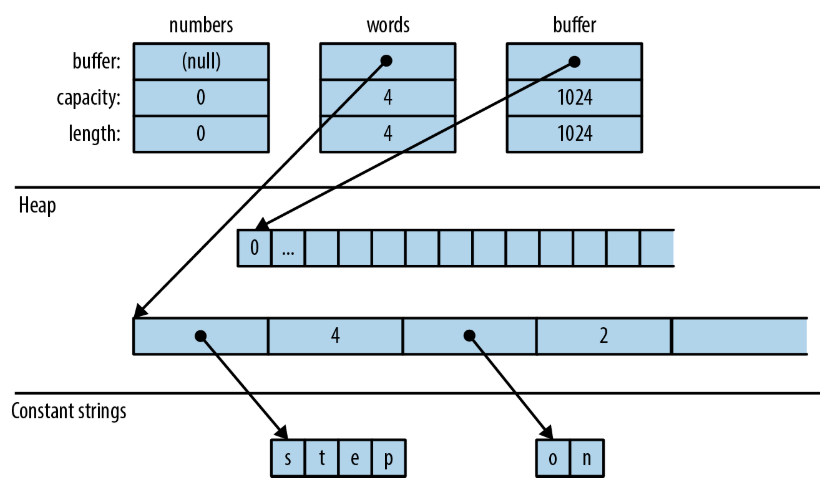
\includegraphics[width=0.9\textwidth]{../img/f16-1.png}
    \caption{vector的内存布局:words的每个元素是一个由指针和长度组成的\&str值}
    \label{f16-1}
\end{figure}

类似于所有集合,\texttt{Vec}实现了\texttt{std::iter::FromIterator},因此你可以对任何迭代器调用\texttt{.collect()}方法来创建一个vector,正如“\nameref{BuildColl}”中所述:
\begin{minted}{Rust}
    // 将一个其他集合转换成vector
    let my_vec = my_set.into_iter().collect::<Vec<String>>();
\end{minted}

\subsection{访问元素}
通过索引访问数组、切片或vector的元素非常直观:
\begin{minted}{Rust}
    // 获取一个元素的引用
    let first_line = &lines[0];

    // 获取一个元素的拷贝 
    let fifth_number = numbers[4];          // 需要Copy
    let second_number = lines[1].clone();   // 需要Clone

    // 获取一个切片的引用
    let my_ref = &buffer[4..12];

    // 获取一个切片的拷贝
    let my_copy = buffer[4..12].to_vec();   // 需要Clone
\end{minted}

当索引越界时所有这些方式都会panic。

Rust对数字类型很挑剔,vector也不例外。vector的长度和索引都是\texttt{usize}类型。尝试使用\texttt{u32}、\texttt{u64}、\texttt{isize}作为vector的索引会导致错误。必要时你可以使用\texttt{n as usize}来转换,见“\nameref{cast}”。

有几种方法提供了便捷地访问vector或切片的特定元素的方法(注意所有的切片方法都能用于数组和vector):
\codeentry{slice.first()}
\hangparagraph{返回\texttt{slice}的第一个元素的引用。返回类型是\texttt{Option<\&T>},因此如果\texttt{slice}为空时返回值为\texttt{None},不为空时返回值为\texttt{Some(\&slice[0])}}:
\begin{minted}{Rust}
    if let Some(item) = v.first() {
        println!("We got one! {}", item);
    }
\end{minted}

\codeentry{slice.last()}
\hangparagraph{和上边相似,不过返回最有一个元素的引用。}

\codeentry{slice.get(index)}
\hangparagraph{返回\texttt{slice[index]}的引用,如果存在的话。如果\texttt{slice}的元素数量小于\texttt{index+1},那么返回\texttt{None}}:
\begin{minted}{Rust}
    let slice = [0, 1, 2, 3];
    assert_eq!(slice.get(2), Some(&2));
    assert_eq!(slice.get(4), None);
\end{minted}

\codeentry{slice.first\_mut(), slice.last\_mut(), slice.get\_mut(index)}
\hangparagraph{与上面的类似,不过借用\texttt{mut}引用:}
\begin{minted}{Rust}
    let mut slice = [0, 1, 2, 3];
    {
        let last = slice.last_mut().unwrap();   // 最后一个元素类型:&mut i32
        assert_eq!(*last, 3);
        *last = 100;
    }
\end{minted}

因为以值返回\texttt{T}意味着移动它,因此访问元素的方法通常返回元素的引用。

一个例外是\texttt{.to\_vec()}方法,它获取拷贝:

\codeentry{slice.to\_vec()}
\hangparagraph{克隆整个切片,返回一个新的vector:}
\begin{minted}{Rust}
    let v = [1, 2, 3, 4, 5, 6, 7, 8, 9];
    assert_eq!(v.to_vec(),
               vec![1, 2, 3, 4, 5, 6, 7, 8, 9]);
    assert_eq!(v[0..6].to_vec(),
               vec![1, 2, 3, 4, 5, 6]);
\end{minted}
\hangparagraph{只有当元素可以拷贝时这个方法才可用,即\texttt{where T: Clone}}

\subsection{迭代}\label{Iteration}
vector和切片可以以值或者以引用迭代,遵循“\nameref{IntoIter}”中介绍的模式:
\begin{itemize}
    \item 迭代\texttt{Vec<T>}会产生\texttt{T}类型的item。元素被逐个移出vector消耗掉。
    \item 迭代\texttt{\&[T; N], \&[T], \&Vec<T>}——即数组、切片或vector的引用——会产生\texttt{\&T}类型的item,每一个item指向一个元素,不会移动元素。
    \item 迭代\texttt{\&mut [T; N], \&mut [T], \&mut Vec<T>}产生\texttt{\&mut T}类型的item。
\end{itemize}

数组、切片和vector还有\texttt{.iter()}和\texttt{.iter\_mut()}方法(见“\nameref{IterMethod}”)创建产生元素的引用的迭代器。

我们将在“\nameref{split}”中介绍一些更有趣的迭代切片的方法。

\subsection{增长和缩减vector}
数组、切片或vector的\emph{长度(length)}是它包含的元素的数量:

\codeentry{slice.len()}
\hangparagraph{返回一个\texttt{slice}的长度,类型为\texttt{usize}。}

\codeentry{slice.is\_empty()}
\hangparagraph{当\texttt{slice}不包含元素时为真(即\texttt{slice.len() == 0})。}

本节剩余的方法都是关于增长和缩减vector。它们不能用于数组和切片,因为它们一旦被创建之后就不能改变大小。

vector的所有元素都存储在一个在堆上分配的连续内存块中。vector的\emph{容量(capacity)}是指当前的内存块中最多能存储的元素数量。\texttt{Vec}通常会替你管理容量,当需要增长时它会自动分配更大的缓冲区并把元素都移动过去。还有一些显式管理容量的方法:

\codeentry{Vec::with\_capacity(n)}
\hangparagraph{创建一个容量为\texttt{n}的新的空vector。}

\codeentry{vec.capacity()}
\hangparagraph{返回\texttt{vec}的容量,类型是\texttt{usize}。\texttt{vec.capacity() >= vec.len()}总是为真。}

\codeentry{vec.reserve(n)}
\hangparagraph{保证vector的剩余空间至少还能再存储\texttt{n}个或更多元素:即\texttt{vec.capacity()}至少是\texttt{vec.len() + n}。如果已经有足够的空间,它不做任何事。否则,它会分配一个更大的缓冲区并且把vector的内容移动过去。}

\codeentry{vec.reserve\_exact(n)}
\hangparagraph{类似于\texttt{vec.reserve(n)},但告诉\texttt{vec}不要为未来的增长分配额外的空间。调用它之后,\texttt{vec.capacity()}等于\texttt{vec.len() + n}。}

\codeentry{vec.shrink\_to\_fit()}
\hangparagraph{当\texttt{vec.capacity()}大于\texttt{vec.len()}时尝试释放额外的内存。}

\texttt{Vec<T>}有很多添加或移除元素的方法,同时改变vector的长度。所有这些方法都以\texttt{mut}引用获取\texttt{self}参数。

下面这两个方法在vector的末尾添加或移除一个元素:

\codeentry{vec.push(value)}
\hangparagraph{把\texttt{value}添加到\texttt{vec}的末尾。}

\codeentry{vec.pop()}
\hangparagraph{移除并返回最后一个元素。返回类型是\texttt{Option<T>}。当vector已经为空时返回\texttt{None},否则返回\texttt{Some(x)}。}

注意\texttt{.push()}以值而不是以引用获取参数。类似的,\texttt{.pop()}返回被弹出的值,而不是引用。本节中剩余的大部分方法也是这样。它们从vector移出或移进值。

这两个方法向vector中添加值或者从vector中移出值:
\codeentry{vec.insert(index, value)}
\hangparagraph{在\texttt{vec[index]}处插入给定的\texttt{value},把\texttt{vec[index..]}中的值都向后移动一个位置来腾出空间。如果\texttt{index > vec.len()}会panic。}

\codeentry{vec.remove(index)}
\hangparagraph{移除并返回\texttt{vec[index]},把\texttt{vec[index+1..]}中的值向左移动一个位置来消除缝隙。}

\texttt{.insert()}和\texttt{.remove()}都很慢,因为有很多元素需要移动。

有四个方法可以将vector的长度调整为指定值:

\codeentry{vec.resize(new\_len, value)}
\hangparagraph{将\texttt{vec}的长度设为\texttt{new\_len}。如果这会增大\texttt{vec}的长度,将会用\texttt{value}的拷贝填充新空间。元素的类型必须实现了\texttt{Clone} trait。}

\codeentry{vec.resize\_with(new\_len, closure)}
\hangparagraph{类似于\texttt{vec.resize},但调用闭包来构造每一个新元素。它可以用于元素没有实现\texttt{Clone}的vector。}

\codeentry{vec.truncate(new\_len)}
\hangparagraph{将\texttt{vec}的长度缩减到\texttt{new\_len},丢弃\texttt{vec[new\_len..]}范围内的所有元素。如果\texttt{vec.len()}小于等于\texttt{new\_len},那么什么也不做。}

\codeentry{vec.clear()}
\hangparagraph{删除\texttt{vec}的所有元素。等价于\texttt{vec.truncate(0)}。}

有四个方法可以一次添加或移除很多元素:

\codeentry{vec.extend(iterable)}
\hangparagraph{将\texttt{iterable}的所有item按顺序添加到\texttt{vec}的末尾。它类似于多值版本的\texttt{.push()}。\texttt{iterable}参数可以是任何实现了\texttt{IntoIterator<Item=T>}。}
\hangparagraph{这个方法如此有用以至于有一个专门的trait \texttt{Extend},所有的标准集合都实现了它。不幸的是,这导致\texttt{rustdoc}将\texttt{.extend()}和其他trait的方法放在生成的HTML底部的一堆方法中,因此当你需要它时很难找到它。你必须记住它!更多内容见“\nameref{extend}”。}

\codeentry{vec.split\_off(index)}
\hangparagraph{类似于\texttt{vec.truncate(index)},除了它返回一个\texttt{Vec<T>}包含\texttt{vec}尾部被移除的元素。它类似于\texttt{.pop()}的多值版本。}

\codeentry{vec.append(\&mut vec2)}
\hangparagraph{这会把\texttt{vec2}的所有元素移动进\texttt{vec},其中\texttt{vec2}是另一个\texttt{Vec<T>}类型的vector。调用之后,\texttt{vec2}变为空。}
\hangparagraph{这类似于\texttt{vec.extend(vec2)},除了调用之后\texttt{vec2}仍然存在,并且容量不变。}

\codeentry{vec.drain(range)}
\hangparagraph{这会从\texttt{vec}中移除范围\texttt{vec[range]},并返回一个迭代被移除元素的迭代器,其中\texttt{range}是一个范围值,例如\texttt{..}或\texttt{0..4}。}

还有一些选择性移除vector元素的古怪方法:
\codeentry{vec.retain(test)}
\hangparagraph{移除所有没有通过给定测试的方法。\texttt{test}参数是一个实现了\texttt{FnMut(\&T) -> bool}的函数或闭包。对于\texttt{vec}的每一个元素,它会调用\texttt{test(\&element)},如果返回\texttt{false},元素将会被移出vector然后丢弃。}
\hangparagraph{不考虑性能的话,这类似于:}
\begin{minted}{Rust}
    vec = vec.into_iter().filter(test).collect();
\end{minted}

\codeentry{vec.dedup()}
\hangparagraph{丢弃相邻的重复元素。它类似于Unix的\texttt{uniq} shell工具。它会扫描\texttt{vec}中寻找相邻的重复元素,然后丢弃掉多余的重复值,只留下一个:}
\begin{minted}{Rust}
    let mut byte_vec = b"Missssssissippi".to_vec();
    byte_vec.dedup();
    assert_eq!(&byte_vec, b"Misisipi");
\end{minted}
\hangparagraph{注意最后的输出中仍然有两个\texttt{'s'}字符。这个方法只移除\emph{相邻的(adjacent)}重复值。为了移除所有的重复值,你有三种选择:调用\texttt{.dedup()}之前先排序vector,将数据移动到一个“\nameref{set}”,或者(为了保持元素原本的顺序)使用这个\texttt{.retain()}技巧:}
\begin{minted}{Rust}
    let mut byte_vec = b"Missssssissippi".to_vec();

    let mut seen = HashSet::new();
    byte_vec.retain(|r| seen.insert(*r));

    assert_eq!(&byte_vec, b"Misp");
\end{minted}
\hangparagraph{这段代码的原理是当集合中已经包含要插入的item时\texttt{.insert()}会返回\texttt{false}。}

\codeentry{vec.dedup\_by(same)}
\hangparagraph{类似于\texttt{vec.dedup()},但它使用函数或者闭包\texttt{same(\&mut elem1, \&mut elem2)},而不是\texttt{==}运算符,来检查两个相邻元素是否被认为相等。}

\codeentry{vec.dedup\_by\_key(key)}
\hangparagraph{类似于\texttt{vec.dedup()},但当\texttt{key(\&mut elem1) == key(\&mut elem2)}时它认为两个元素相等。}
\hangparagraph{例如,如果\texttt{errors}是一个\texttt{Vec<Box<dyn Error>>},你可以写:}
\begin{minted}{Rust}
    // 移除消息重复的错误。
    errors.dedup_by_key(|err| err.to_string());
\end{minted}

这一节介绍的所有方法中,只有\texttt{.resize()}可能会拷贝值。其他的通过移动值来工作。

\subsection{连接}
两个方法可以用于\emph{数组的数组(array of array)},即元素类型是数组、切片、vector的数组、切片、vector:

\codeentry{slices.concat()}
\hangparagraph{返回一个所有切片连接成的vector:}
\begin{minted}{Rust}
    assert_eq!([[1, 2], [3, 4], [5, 6]].concat(),
               vec![1, 2, 3, 4, 5, 6]);
\end{minted}

\codeentry{slices.join(\&separator)}
\hangparagraph{同上,除了会在切片之间插入\texttt{separator}的拷贝:}
\begin{minted}{Rust}
    assert_eq!([[1, 2], [3, 4], [5, 6]].join(&0),
               vec![1, 2, 0, 3, 4, 0, 5, 6]);
\end{minted}

\subsection{切分}\label{split}
很容易一次获得数组、切片、vector中的很多元素的非\texttt{mut}引用:
\begin{minted}{Rust}
    let v = vec![0, 1, 2, 3];
    let a = &v[i];
    let b = &v[j];

    let mid = v.len() / 2;
    let front_half = &v[..mid];
    let back_half = &v[mid..];
\end{minted}

但一次获得多个\texttt{mut}引用不是这么容易:
\begin{minted}{Rust}
    let mut v = vec![0, 1, 2, 3];
    let a = &mut v[i];
    let b = &mut v[j];  // error: 不能同时借用`v`的
                        // 多个可变引用。

    *a = 6;             // 引用`a`和`b`在这里使用了,
    *b = 7;             // 因此它们的生命周期一定会重叠。
\end{minted}

Rust禁止这样,因为如果\texttt{i == j},那么\texttt{a}和\texttt{b}将是同一个整数的两个\texttt{mut}引用,这违背了Rust的安全性的规则。(见“\nameref{ShareVSMut}”)。

Rust有几个方法可以一次借用数组、切片、vector的两个或更多元素的\texttt{mut}引用。和上面的代码不同,这些方法是安全的,因为它们从设计上保证了只会把数组分割成\emph{非重叠(nonoverlapping)区域}。这些方法也可以用于非\texttt{mut}切片,因此它们有\texttt{mut}和非\texttt{mut}版本。

\begin{figure}[htbp]
    \centering
    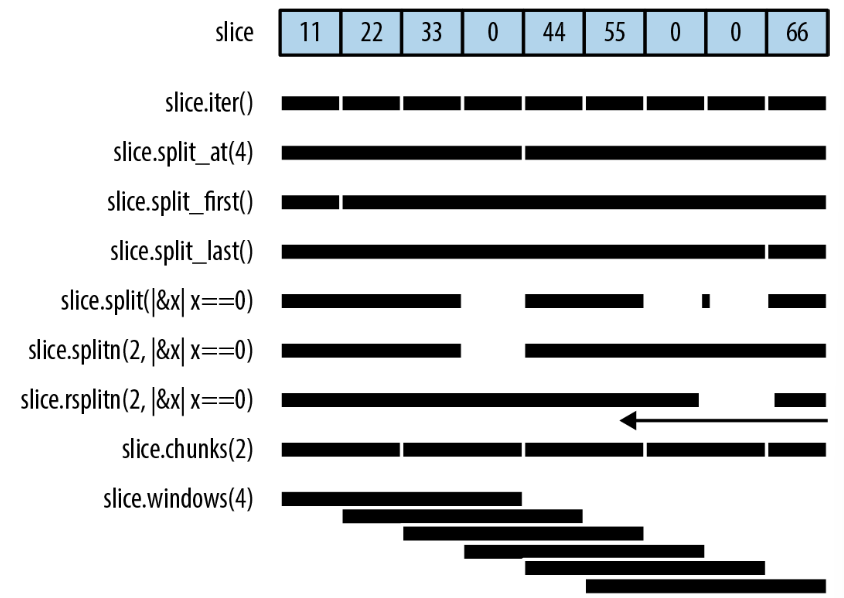
\includegraphics[width=0.9\textwidth]{../img/f16-2.png}
    \caption{分隔方法展示(注意:\texttt{slice.split()}输出中的小矩形是空的切片,因为两侧都是分隔符,\texttt{rsplitn}的输出是按照从后往前的顺序,这一点和其他的不同。}
    \label{f16-2}
\end{figure}

这些方法中没有一个会直接修改数组、切片或vector;它们都返回部分数据的引用:
\codeentry{slice.iter(), slice.iter\_mut()}
\hangparagraph{产生\texttt{slice}的每个元素的引用。我们在“\nameref{Iteration}”中已经介绍过它们。}

\codeentry{slice.split\_at(index), slice.split\_at\_mut(index)}
\hangparagraph{将一个切片划分为两个,返回一个pair。\texttt{slice.split\_at(index)}等价于\texttt{(\&slice[..index], \&slice[index..])}。如果\texttt{index}越界会panic。}

\codeentry{slice.split\_first(), slice.split\_first\_mut()}
\hangparagraph{也返回一个pair:第一个元素的引用(\texttt{slice[0]})和其余所有元素的切片引用(\texttt{slice[1..]})。}
\hangparagraph{\texttt{.spilt\_first()}的返回值类型是\texttt{Option<(\&T, \&[T])>};如果\texttt{slice}为空,返回\texttt{None}。}

\codeentry{slice.split\_last(), slice.split\_last\_mut()}
\hangparagraph{类似上一个,不过划分出最后一个元素而不是第一个。}
\hangparagraph{\texttt{.split\_last()}的返回类型是\texttt{Option<(\&T, \&[T])>}。}

\codeentry{slice.split(is\_sep), slice.split\_mut(is\_sep)}
\hangparagraph{将\texttt{slice}切分成一个或更多子切片,使用函数或闭包\texttt{is\_sep}来判断在哪里切分。它们返回一个迭代子切片的迭代器。}
\hangparagraph{当你消耗迭代器时,它会对切片中的每个元素调用\texttt{is\_sep(\&element)}。如果\texttt{is\_sep(\&element)}返回\texttt{true},那么这个元素就是一个分隔符。分隔符不包含在任何输出的字切片中。}
\hangparagraph{输出总是包含至少一个子切片,每有一个分隔符就加一个子切片。如果有相邻的分隔符或者\texttt{slice}的两端是分隔符都会产生空的子切片。}

\codeentry{slice.rsplit(is\_sep), slice.rsplit\_mut(is\_sep)}
\hangparagraph{类似于\texttt{slice}和\texttt{slice\_mut},但从最后一个切片开始。}

\codeentry{slice.splitn(n, is\_sep), slice.splitn\_mut(n, is\_sep)}
\hangparagraph{类似上面的方法,不过最多产生\texttt{n}个子切片。当发现了前\texttt{n-1}个切片之后就不会再调用\texttt{is\_sep}。最后一个字切片将包含剩余的所有元素。}

\codeentry{slice.rsplitn(n, is\_sep), slice.rsplitn\_mut(n, is\_sep)}
\hangparagraph{类似于\texttt{.splitn()}和\texttt{.splitn\_mut()},除了反向扫描切片。就是说,这个方法会在切片中\emph{最后}\texttt{n-1}个分隔符处切分,而不是前\texttt{n-1}个,并且从尾部开始产生子切片。}

\codeentry{slice.chunks(n), slice.chunks\_mut(n)}
\hangparagraph{返回一个产生长度为\texttt{n}的非重叠子切片的迭代器。如果\texttt{n}不能整除\texttt{slice.len()},最后一个块的元素数量将小于\texttt{n}。}

\codeentry{slice.rchunks(n), slick.rchunks\_mut(n)}
\hangparagraph{类似于\texttt{slice.chunks()}和\texttt{slice.chunks\_mut()},但是从切片的尾部开始。}

\codeentry{slice.chunks\_exact(n), slice.chunks\_exact\_mut(n)}
\hangparagraph{返回一个产生长度为\texttt{n}的非重叠子切片的迭代器。如果\texttt{n}不能整除\texttt{slice.len()},最后一个块(元素数量小于\texttt{n})可以通过结果的\texttt{remainder()}方法获得。}

\codeentry{slice.rchunks\_exact(n), slice.rchunks\_exact\_mut(n)}
\hangparagraph{类似于\texttt{slice.chunks\_exact}和\texttt{slice.chunks\_exact\_mut},但从切片的尾部开始。}

还有一些其他迭代子切片的方法:
\codeentry{slice.windows(n)}
\hangparagraph{返回一个效果类似于“滑动窗口”的迭代器。它产生\texttt{slice}中相邻的\texttt{n}个元素的子切片。第一个产生的值是\texttt{\&slice[0..n]},第二个是\texttt{\&slice[1..n+1]},以此类推。}
\hangparagraph{如果\texttt{n}大于\texttt{slice}的长度,将不会产生切片。如果\texttt{n}是0,这个方法会panic。}
\hangparagraph{例如,如果\texttt{days.len() == 31},那么我们可以调用\texttt{days.windows(7)}产生\texttt{days}中所有7天的区间。}
\hangparagraph{在探索数据列的变化趋势时一个大小为2的滑动窗口会很有用:}
\begin{minted}{Rust}
    let changes = daily_high\_temperatures
                      .windows(2)           // 获得相邻天的温度
                      .map(|w| w[1] - w[0]) // 温度改变了多少
                      .collect::<Vec<_>>();
\end{minted}
\hangparagraph{因为子切片是重叠的,所以这个方法没有返回\texttt{mut}引用的版本。}

\subsection{交换}

\section{\texttt{HashMap<K, V>}和\texttt{BTreeMap<K, V>}}

\subsection{条目}\label{entry}
    \chapter{字符串与文本}\label{ch17}

\emph{The string is a stark data structure and everywhere it is passed there is much duplication of process. It is a perfect vehicle for hiding information.}
\begin{flushright}
    ——Alan Perlis, epigram \#34
\end{flushright}

我们已经使用过了Rust中的主要文本类型:\texttt{String}、\texttt{str}和\texttt{char}。在“\nameref{string}”中,我们介绍了字符和字符串字面量的语法并且展示了字符串在内存中如何表示。在本章中,我们将更加详细地介绍文本。

在本章中:
\begin{enumerate}
    \item 我们会提供一些Unicode的背景知识,帮助你更好地理解标准库的设计。
    \item 我们会介绍\texttt{char}类型,它表示单个Unicode码点。
    \item 我们会介绍\texttt{String}和\texttt{str}类型,它们表示有所有权的和借用的Unicode字符序列。它们有非常多的方法用于构建、搜索、修改、迭代它们的内容。
    \item 我们会介绍Rust的字符串格式化设施,例如\texttt{println!}和\texttt{format!}宏。你可以编写自己的用于字符串格式化的宏,以及扩展它们来支持你自定义的类型。
    \item 我们会给出Rust中正则表达式支持的一个概述。
    \item 最后我们会讨论为什么Unicode规范化很重要,并展示如何在Rust中实现它。
\end{enumerate}

\section{Unicode背景知识}

本书是关于Rust的,而不是关于Unicode的,事实上已经有整本专门介绍它的书了。但Rust的字符和字符串类型被设计为Unicode。这里有一些有助于理解Rust的Unicode知识。

\subsection{ASCII, Latin-1, Unicode}
在所有ASCII码点范围(\texttt{0}到\texttt{0x7f})内Unicode和ASCII完全相同:例如,这两种编码中字符\texttt{*}都是码点\texttt{42}。

\subsection{UTF-8}\label{utf8}

\section{字符(\texttt{char})}

\section{\texttt{String}和\texttt{str}}

\subsection{创建\texttt{String}值}

\subsection{简单的视图}

\subsection{附加和插入文本}\label{AppendText}

\section{格式化}\label{format}

\section{正则表达式}

\subsection{基本正则使用}

\subsection{惰性构建正则值}\label{LazyRegex}

    \chapter{输入输出}\label{ch18}

\emph{Doolittle: What concrete evidence do you have that you exist?
Bomb \#20: Hmmmm... well... I think, therefore I am.
Doolittle: That’s good. That’s very good. But how do you know that anything else exists?
Bomb \#20: My sensory apparatus reveals it to me.}

\begin{flushright}
    ——Dark Star
\end{flushright}

Rust中有关输入输出的特性围绕着三个trait:\texttt{Read}、\texttt{BufRead}、\texttt{Write}来组织:
\begin{enumerate}
    \item 实现了\texttt{Read}的值有读取字节输入的方法。它们被称为\emph{读者(reader)}。
    \item 实现了\texttt{BufRead}的值是\emph{buffered reader(有缓存的读者)}。它们支持\texttt{Read}的所有方法,加上读取文本的一行的方法,等等。
    \item 实现了\texttt{Write}的值支持字节和UTF-8文本输出。它们被称为\emph{写者(writer)}。
\end{enumerate}

\autoref{f18-1}展示了这三个trait以及一些reader和writer类型的示例。

在本章中,我们将解释如何使用这些trait和它们的方法,包括图中出现的reader和writer类型,还有一些其他的和文件、终端、网络交互的方法。

\begin{figure}[htbp]
    \centering
    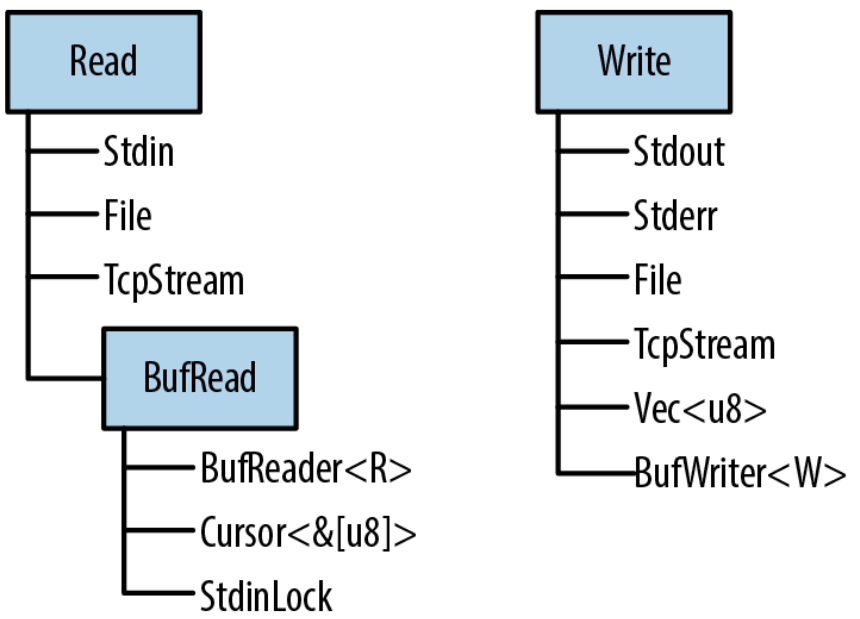
\includegraphics[width=0.8\textwidth]{../img/f18-1.png}
    \caption{Rust的三个主要的I/O trait以及一些实现了它们的类型}
    \label{f18-1}
\end{figure}

\section{Reader和Writer}

\emph{Reader}是你的程序可以从中读取字节的值。例如:
\begin{enumerate}
    \item 使用\texttt{std::fs::File::open(filename)}打开的文件
    \item 用于从网络中接收数据的\texttt{std::net::TcpStream}
    \item 进程用来读取标准输入的\texttt{std::io::stdin()}
    \item \texttt{std::io::Cursor<\&[u8]>}和\texttt{std::io::Cursor<Vec<u8>>}值,它们是从内存中的字节数组或vector中“读取”数据的reader
\end{enumerate}

\emph{Writer}是你的程序可以向其中写入字节的值。例如:
\begin{enumerate}
    \item 使用\texttt{std::fs::File::create(filename)}打开的文件
    \item 用于向网络中发送数据的\texttt{std::net::TcpStream}
    \item 用于写入到终端的\texttt{std::io::stdout()}和\texttt{std::io::stderr()}
    \item \texttt{Vec<u8>},它也是一个writer,它的\texttt{write}方法把数据附加到尾部
    \item std::io::Cursor<Vec<u8>>,类似于上面,但允许你同时读取和写入数据,并可以在vector中定位到不同位置
    \item std::io::Cursor<\&mut [u8]>,和\texttt{std::io::Cursor<Vec<u8>>}很像,除了它不能让缓冲区增长,因为它只是已经存在的字节数组的切片
\end{enumerate}

因为有为reader和writer设计的标准trait(\texttt{std::io::Read}和\texttt{std::io::Write}),所以编写可以处理多种输入输出通道的泛型代码是非常普遍的。例如,这里有一个函数拷贝任意reader中的所有字节到任意writer:
\begin{minted}{Rust}
    use std::io::{self, Read, Write, ErrorKind};

    const DEFAULT_BUF_SIZE: usize = 8 * 1024;

    pub fn copy<R: ?Sized, W: ?Sized>(reader: &mut R, writer: &mut W)
        -> io::Result<u64>
        where R: Read, W: Write
    {
        let mut buf = [0; DEFAULT_BUF_SIZE];
        let mut written = 0;
        loop {
            let len = match reader.read(&mut buf) {
                Ok(0) => return Ok(written),
                Ok(len) => len,
                Err(ref e) if e.kind() == ErrorKind::Interrupted => continue,
                Err(e) => return Err(e),
            };
            writer.write_all(&buf[..len])?;
            written += len as u64;
        }
    }
\end{minted}

这是Rust的标准库中的\texttt{std::io::copy()}的实现。因为它是泛型的,你可以使用它从\texttt{File}中读取数据然后写入到\texttt{TcpStream},或者从\texttt{Stdin}读取,然后写入到内存中的\texttt{Vec<u8>},等等。

如果你看不明白这里的错误处理代码,请复习\hyperref[ch07]{第7章}。我们将在接下来的页面中一直使用\texttt{Result}类型;掌握它的工作原理很重要。

这三个\texttt{std::io}的trait:\texttt{Read}、\texttt{BufRead}、\texttt{Write},以及\texttt{Seek}如此常用,以至于有一个只包含这些trait的\texttt{prelude}模块:
\begin{minted}{Rust}
    use std::io::prelude::*;
\end{minted}

本章中你还会见到它一到两次。我们通常也习惯于导入\texttt{std::io}模块自身:
\begin{minted}{Rust}
    use std::io::{self, Read, Write, ErrorKind};
\end{minted}

这里的\texttt{self}关键字声明了\texttt{io}作为\texttt{std::io}模块的一个别名。这样,\texttt{std::io::Result}和\texttt{std::io::Error}可以用\texttt{io::Result}和\texttt{io::Error}更精确地表示出来,等等。

\subsection{Reader}
\texttt{std::io::Read}有几个方法用于读取数据。所有这些方法都通过\texttt{mut}引用获取self参数。

\codeentry{reader.read(\&mut buffer)}
\hangparagraph{从数据源读取一些字节,并存储到给定的\texttt{buffer}中。\texttt{buffer}参数的类型是\texttt{\&mut [u8]}。它最多读取\texttt{buffer.len()}个字节。}
\hangparagraph{返回类型是\texttt{io::Result<u64>},它是\texttt{Result<u64, io::Error>}的类型别名。当成功时,\texttt{u64}值是读取到的字节数——可能等于或着小于\texttt{buffer.len()},\emph{即使还有更多的数据可以读取}。\texttt{Ok(0)}意味着没有更多的输入可以读取。}
\hangparagraph{当出错时,\texttt{.read()}返回\texttt{Err(err)},其中\texttt{err}是一个\texttt{io::Error}值。\texttt{io::Error}是可打印的,为了便于阅读;对于程序来讲,它有一个\texttt{.kind()}方法返回一个\texttt{io::ErrorKind}类型的错误码。这个枚举的成员有例如\texttt{PermissionDenied}和\texttt{ConnectionReset}的名称。大多数的错误类型都不能被忽略,但有一种错误应该进行特殊处理。\texttt{io::ErrorKind::Interrupted}对应Unix的错误码\texttt{EINTR},它意味着读取过程恰好被一个信号打断。除非你的程序想设计为根据信号做一些聪明的操作,否则它应该简单地重试读取操作。上一节中的\texttt{copy()}的代码,就是一个例子。}
\hangparagraph{如你所见,\texttt{.read()}方法非常底层,甚至直接继承了底层操作系统的怪癖。如果你要为一个新的数据源类型实现\texttt{Read} trait,这会赋予你极大的灵活性。但如果你尝试读取一些数据,就会非常难受。因此,Rust提供了几个更高级的便捷方法。它们都有基于\texttt{.read()}的默认实现。它们都处理了\texttt{ErrorKind::Interrupted},因此你不需要再处理。}

\codeentry{reader.read\_to\_end(\&mut byte\_vec)}
\hangparagraph{读取reader种剩余的所有输入,将读到的数据附加到\texttt{byte\_vec}尾部,\texttt{byte\_vec}是一个\texttt{Vec<u8>}。返回一个\texttt{io::Result<uszie>},表示读取到的字节数。}
\hangparagraph{这个方法读取的数据的大小没有限制,因此不要将它用于不受信任的源。(你可以使用\texttt{.take()}方法施加限制,如后文所述。}

\codeentry{reader.read\_to\_string(\&mut string)}
\hangparagraph{和上面相同,不过把数据附加到给定的\texttt{String}。如果流不是有效的UTF-8,它会返回一个\texttt{ErrorKind::InvalidData}错误。}
\hangparagraph{在一些编程语言中,字节输入和字符输入由不同的类型来处理。如今,UTF-8占据主导地位,Rust承认这一事实标准,并且完全支持UTF-8。其他字符集由开源的\texttt{encoding} crate提供支持。}

\codeentry{reader.read\_exact(\&mut buf)}
\hangparagraph{读取恰好足够的数据来填充给定的缓冲区。参数的类型是\texttt{\&mut [u8]},如果在读取够\texttt{buf.len()}个字节之前reader的数据就已经耗光,那么它会返回一个\texttt{ErrorKind::UnexpectedEof}错误。}

上面这些是\texttt{Read} trait的主要方法。除此之外,还有三个以值获取\texttt{reader}的适配器方法,将它转换为一个迭代器或者一个不同的reader:

\codeentry{reader.bytes()}
\hangparagraph{返回一个输入流的字节的迭代器。item的类型是\texttt{io::Result<u8>},因此每一个字节都需要进行错误检查。另外,它会逐字节调用\texttt{reader.read()},因此如果reader没有缓存的话会非常低效。}

\codeentry{reader.chain(reader2)}
\hangparagraph{返回一个新的reader,首先产生\texttt{reader}的所有输入,然后产生\texttt{reader2}的所有输入。}

\codeentry{reader.take(n)}
\hangparagraph{返回一个新的reader,从和\texttt{reader}相同的数据源读取数据,但最多只读取\texttt{n}个字节。}

没有关闭reader的方法。reader和writer通常实现了\texttt{Drop},因此它们会自动关闭。

\subsection{Buffered Reader}
出于性能考虑,reader和writer可以进行\emph{缓存(buffer)},意思是它们有一块内存(缓冲区)用来存储一些输入或输出数据。这样可以减少系统调用的次数,如\autoref{f18-2}所示。在这个例子中,应用调用\texttt{.read\_line()}方法从\texttt{BufReader}中读取数据,\texttt{BufReader}从操作系统获取更大块的输入。

\begin{figure}[htbp]
    \centering
    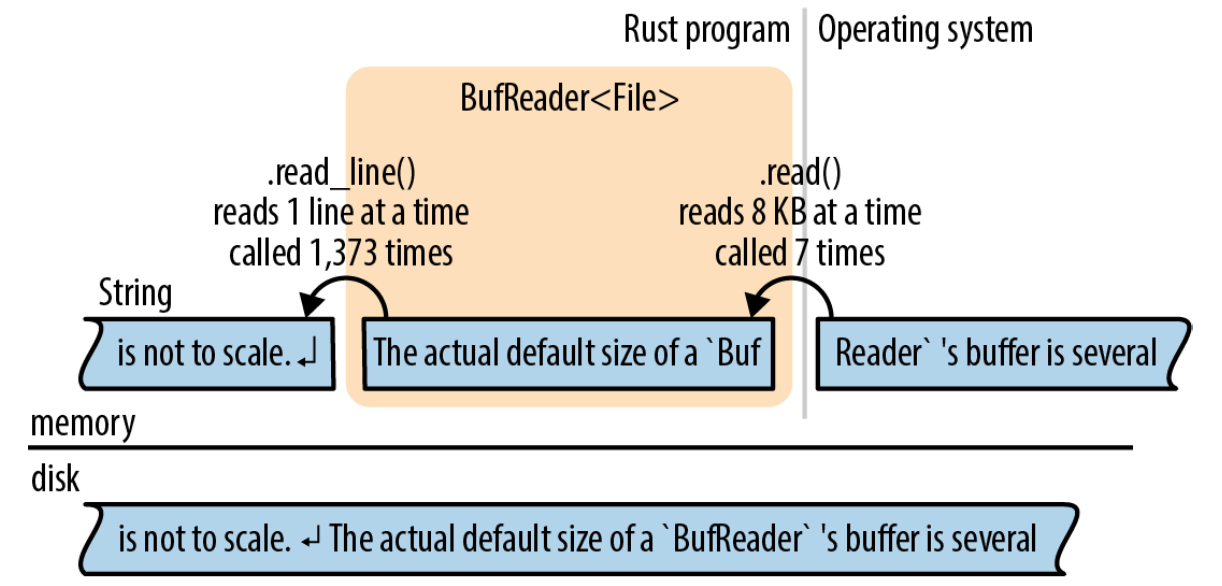
\includegraphics[width=0.9\textwidth]{../img/f18-2.png}
    \caption{一个有缓冲的文件reader}
    \label{f18-2}
\end{figure}

这张图并不是按比例的,一个\texttt{BufReader}的实际大小是几千字节,因此一次系统的\texttt{read}调用可以提供上百次\texttt{.read\_line()}调用。这么做之所以能提高性能是因为系统调用很慢。(如图所示,操作系统也有一个缓冲区,原因与此相同:系统调用很慢,但从磁盘读取数据更慢。)

有缓冲的reader实现了\texttt{Read}和另一个trait \texttt{BufRead},它添加了下面的方法:

\codeentry{reader.read\_line(\&mut line)}
\hangparagraph{读取一行文本并将它附加到\texttt{line},\texttt{line}是一个\texttt{String}。行尾的换行符\texttt{'\\n'}}也会包含在\texttt{line}中。如果输入中有Windows风格的换行符\texttt{"\\r\\n"},这两个字符都会包含进\texttt{line}。
\hangparagraph{返回值是一个\texttt{io::Result<usize>},代表读取到的字节数,包括行尾的换行符。}
\hangparagraph{如果reader到达输入结尾,\texttt{line}会保持不变,并返回\texttt{Ok(0)}。}

\codeentry{reader.lines()}
\hangparagraph{返回一个迭代输入中每一行的迭代器。item的类型是\texttt{io::Result<String>}。换行符\emph{不}包含在字符串中。如果输入中有Windows风格的换行符\texttt{"\\r\\n"},这两个字符都会被丢球。}
\hangparagraph{这个方法几乎总是你需要的文本输入方法。下面的两节会通过例子展示如何使用它。}

\codeentry{reader.read\_until(stop\_byte, \&mut byte\_vec), reader.split(stop\_byte)}
\hangparagraph{这两个方法类似于\texttt{.read\_line()}和\texttt{.lines()},但是是面向字节的,产生\texttt{Vec<u8>}而不是\texttt{String}。你可以选择终止符\texttt{stop\_byte}。}

\texttt{BufRead}还提供两个底层的方法\texttt{.fill\_buf()}和\texttt{.consume(n)},用来直接访问reader的内部缓冲区。更多有关这些方法的信息,可以查阅在线文档。

接下来的两节详细介绍了有缓冲的reader。

\subsection{读取行}\label{ReadLines}
这里有一个实现了Unix \texttt{grep}工具的函数。它搜索文本的每一行,文本通常通过管道从另一个命令输入。对于一个给定的字符串:
\begin{minted}{Rust}
    use std::io;
    use std::io::prelude::*;

    fn grep(target: &str) -> io::Result<()> {
        let stdin = io::stdin();
        for line_result in stdin.lock().lines() {
            let line = line_result?;
            if line.contains(target) {
                println!("{}", line);
            }
        }
        Ok(())
    }
\end{minted}

因为我们想要调用\texttt{.lines()},所以我们需要一个实现了\texttt{BufRead}的输入源。在这个例子中,我们调用了\texttt{io::stdin()}来获取通过管道传入的数据。然而,Rust标准库使用了一个mutex来保护\texttt{stdin},我们调用\texttt{.lock()}来锁住\texttt{stdin}以让当前的线程独占使用,它返回一个实现了\texttt{BufRead}的\texttt{StdinLock}值。在循环的结尾,\texttt{StdinLock}被丢弃,释放mutex。(如果没有mutex,那么如果两个线程同时从\texttt{stdin}中读取数据,会导致未定义行为。C里也有这个问题,它通过这种方式解决它:C中所有的输入和输出函数会在幕后获取一个锁。Rust中唯一的不同就是锁是API的一部分。)

函数的剩余部分非常直观:它调用\texttt{.lines()}并迭代返回的迭代器。因为这个迭代器产生\texttt{Result}值,所以我们使用\texttt{?}操作符来检查错误。

假设我们想进一步扩展我们的\texttt{grep}程序,让它支持搜索磁盘中的文件。我们可以把函数修改为泛型的:
\begin{minted}{Rust}
    fn grep<R>(target: &str, reader: R) -> io::Result<()>
        where R: BufRead
    {
        for line_result in reader.lines() {
            let line = line_result?;
            if line.contains(target) {
                println!("{}", line);
            }
        }
        Ok(())
    }
\end{minted}

现在我们可以向它传递一个\texttt{StdinLock}或者一个有缓存的\texttt{File}:
\begin{minted}{Rust}
    let stdin = io::stdin();
    grep(&target, stdin.lock())?;   // ok

    let f = File::open(file)?;
    grep(&target, BufReader::new(f))?;  // ok
\end{minted}

注意\texttt{File}并不是自动缓存的。\texttt{File}实现了\texttt{Read}但没有实现\texttt{BufRead}。然而,很容易为\texttt{File}或者其他任何无缓存的reader创建一个有缓存的reader。\texttt{BufReader::new(reader)可以实现这个功能。(为了设置缓冲区的大小,可以使用\texttt{BufReader::with\_capacity(size, reader)}。}

在大多数语言中,文件都是默认有缓存的。如果你想要无缓存的输入或输出,你必须知道如何关闭缓存。在Rust中,\texttt{File}和\texttt{BufReader}是两个单独的库特性,因为有时你可能需要没有缓冲的文件,或者需要缓存文件之外的内容(例如,你可能会想要缓存来自网络的输入)。

包含错误处理和一些参数解析的完成的程序,如下所示:
\begin{minted}{Rust}
    // grep - 搜索stdin或文件中匹配给定string的行
    use std::error::Error;
    use std::io::{self, BufReader};
    use std::io::prelude::*;
    use std::fs::File;
    use std::path::PathBuf;

    fn grep<R>(target: &str, reader: R) -> io::Result<()>
        where R: BufRead
    {
        for line_result in reader.lines() {
            let line = line_result?;
            if line.contains(target) {
                println!("{}", line);
            }
        }
        Ok(())
    }

    fn grep_main() -> Result<(), Box<dyn Error>> {
        // 获取命令行参数。第一个参数是要搜索的字符串;
        // 剩余的是文件名。
        let mut args = std::env::args().skip(1);
        let target = match args.next() {
            Some(s) => s,
            None => Err("usage: grep PATTERN FILE...")?
        };
        let files: Vec<PathBuf> = args.map(PathBuf::from).collect();

        if files.is_empty() {
            let stdin = io::stdin();
            grep(&target, stdin.lock())?;
        } else {
            for file in files {
                let f = File::open(file)?;
                grep(&target, BufReader::new(f))?;
            }
        }

        Ok(())
    }

    fn main() {
        let result = grep_main();
        if let Err(err) = result {
            eprintln!("{}", err);
            std::process::exit(1);
        }
    }
\end{minted}

\subsection{收集行}
包括\texttt{.lines()}在内的几个reader方法返回产生\texttt{Result}的迭代器。当你第一次尝试将一个文件的每一行收集到一个很大的vector中时,你可能会遇到需要摆脱\texttt{Result}的问题:
\begin{minted}{Rust}
    // ok,但不是你想要的
    let results: Vec<io::Result<String>> = reader.lines().collect();

    // error: 不能将Result的集合转换成Vec<String>
    let lines: Vec<String> = reader.lines().collect();
\end{minted}

第二次尝试不能编译:哪里出错了?直观的解决方法是编写一个\texttt{for}循环并为每一个item检查错误:
\begin{minted}{Rust}
    let mut lines = vec![];
    for line_result in reader.lines() {
        lines.push(line_result?);
    }
\end{minted}

不错;但这里如果使用\texttt{.collect()}会更好,并且我们确实可以这么做。我们只需要知道需要什么样的类型:
\begin{minted}{Rust}
    let lines = reader.lines().collect::<io::Result<Vec<String>>>()?;
\end{minted}

为什么这能工作?标准库里为\texttt{Result}包含了一个\texttt{FromIterator}的实现——在在线文档中容易忽略——让这变为了可能:
\begin{minted}{Rust}
    impl<T, E, C> FromIterator<Result<T, E>> for Result<C, E>
        where C: FromIterator<T>
    {
        ...
    }
\end{minted}
这个签名需要仔细阅读,但它是一个漂亮的技巧。假设\texttt{C}是任意集合类型,例如\texttt{Vec}或者\texttt{HashSet}。只要我们已经知道了如何从一个产生\texttt{T}值的迭代器构建一个\texttt{C},我们就可以从一个产生\texttt{Result<T, E>}值的迭代器构建一个\texttt{Result<C, E>}。我们只需要遍历迭代器产生的值,用其中的\texttt{Ok}值构建集合,但如何遇到了一个\texttt{Err},就停止并传递它。

换句话说,\texttt{io::Result<Vec<String>>}是一个集合类型,所以\texttt{.collect()}方法可以创建并填充这种类型的值。

\subsection{Writer}
正如我们所见,使用方法就基本可以完成输入。输出有一些不同。

在整本书中,我们都在使用\texttt{println!()}来产生普通文本输出:
\begin{minted}{Rust}
    println!("Hello, world!");

    println!("The greatest common divisor of {:?} is {}", numbers, d);

    println!();     // 打印空白行
\end{minted}

还有一个\texttt{print!()}宏,它不会在最后加上一个换行符,\texttt{eprintln!}和\texttt{eprint!}宏写入到标准错误流。这些函数的格式化代码都和\texttt{format!}宏一样,见“\nameref{format}”。

为了将输出送到一个writer,使用\texttt{write!()}和\texttt{writeln!()}宏。它们与\texttt{print!()}和\texttt{println!()}基本相同,除了两个不同之处:
\begin{minted}{Rust}
    writeln!(io::stderr(), "error: world not helloable")?;

    writeln!(&mut byte_vec, "The greatest common divisor of {:?} is {}", numbers, d)?;
\end{minted}

一个不同之处是\texttt{write}宏有一个额外的第一个参数:writer。另一个不同是它们返回一个\texttt{Result},因此必须进行错误处理。这就是为什么我们在每一行的结尾都使用了\texttt{?}运算符。

\texttt{print}宏不返回一个\texttt{Result},如果写入失败它们会直接panic。因为它们会写入到终端,这是很少见的场景。

\texttt{Write} trait有这些方法:
\codeentry{writer.write(\&buf)}
\hangparagraph{将切片\texttt{buf}中的字节写入到底层的流中。它返回一个\texttt{io::Result<usize>}。成功时,它返回写入的字节数量,可能会小于\texttt{buf.len()},取决于流。}
\hangparagraph{类似于\texttt{Reader::read()},这是一个你应该避免直接使用的底层方法。}

\codeentry{writer.write\_all(\&buf)}
\hangparagraph{写入切片\texttt{buf}中的所有字节。返回\texttt{Result<()>}。}

\codeentry{writer.flush()}
\hangparagraph{冲洗底层流中所有缓存的数据。返回\texttt{Result<()>}。}
\hangparagraph{注意尽管\texttt{println!}和\texttt{eprintln!}宏会自动冲洗标准输出和标准错误流,但\texttt{print!}和\texttt{eprint!}不会。使用它们之后你可能需要手动调用\texttt{flush()}。}

类似于reader,writer也是在丢弃时自动关闭。

类似于\texttt{BufReader::new(reader)}为任意reader添加缓存,\texttt{BufWriter::new(writer)}为任意writer添加缓存:
\begin{minted}{Rust}
    let file = File::create("tmp.txt")?;
    let writer = BufWriter::new(file);
\end{minted}

为了设置缓冲区的大小,使用\texttt{BufWriter::with\_capacity(size, writer)。}

当\texttt{BufWriter}被丢弃时,它剩余的所有被缓存的数据都会被写入到底层的writer。然而,如果这次写入时出现了错误,这个错误会被\emph{忽略}。(因为这个错误是在\texttt{BufWriter}的\texttt{.drop()}方法中发生,没有汇报错误的地方。)为了保证你的应用能够注意到所有的输出错误,可以在drop有缓存的writer之前手动调用\texttt{.flush()}。

\subsection{File}\label{file}
我们已经看到过两种打开文件的方式:
\codeentry{File::open(filename)}
\hangparagraph{打开一个已存在的文件。它返回一个\texttt{io::Result<File>},如果文件不存在将返回一个错误。}

\codeentry{File::create(filename)}
\hangparagraph{创建一个新的文件用于写入。如果已经有同名文件,它会被截断。}

注意\texttt{File}类型在文件系统模块\texttt{std::fs}中,而不是在\texttt{std::io}中。

当这两个文件都不符合要求时,你可以使用\texttt{OpenOptions}来指定额外的期望行为:
\begin{minted}{Rust}
    use std::fs::OpenOptions;

    let log = OpenOptions::new()
        .append(true)   // 如果文件存在,就追加到末尾
        .open("server.log")?;

    let file = OpenOptions::new()
        .write(true)
        .create_new(true)   // 如果文件存在就失败
        .open("new_file.txt")?;
\end{minted}

方法\texttt{.append(), .write(), .create\_new()}等,被设计用来进行类似这样的链式调用:每一个都返回\texttt{self}。这种链式方法的设计模式在Rust中太过普遍以至于有一个专门的名字:它被称为\emph{builder(构建器)}。\texttt{std::process::Command}是另一个例子。更多关于\texttt{OpenOptions}的细节可以查阅在线文档。

\texttt{File}被打开后,它的行为就类似于其他的reader和writer。如果需要的话你可以添加一个缓冲区。当你drop一个\texttt{File}时它会自动关闭。

\subsection{Seek}
\texttt{File}还实现了\texttt{Seek} trait,它意味着你可以在一个\texttt{File}中跳来跳去,而不是只能从开始单调地读到尾。\texttt{Seek}的定义类似如下:
\begin{minted}{Rust}
    pub trait Seek {
        fn seek(&mut self, pos: SeekFrom) -> io::Result<u64>;
    }

    pub enum SeekFrom {
        Start(u64),
        End(i64),
        Current(i64)
    }
\end{minted}

得益于这个枚举,\texttt{seek}方法变得很有表达力:使用\texttt{file.seek(SeekFrom::Start(0))}来定位到开始,使用\texttt{file.seek(SeekFrom::Current(-8))}来回退一些字节,等等。

在一个文件中定位很慢。不管你是在硬盘还是固态盘(SSD)上,定位都要消耗和读取几M数据一样长的时间。

\subsection{其他Reader和Writer类型}
到目前为止,本章中使用了\texttt{File}作为主要的示例,但还有很多其他有用的reader和writer类型:
\codeentry{io::stdin()}
\hangparagraph{返回一个标准输入流的reader。它的类型是\texttt{io::Stdin}。因为它被多个线程共享,所以每一次读取需要请求并释放mutex。}
\hangparagraph{\texttt{Stdin}有一个\texttt{.lock()}方法获取mutex并返回一个\texttt{io::StdinLock},这是一个有缓存的reader,它会持有mutex,直到它被丢弃。因此对\texttt{StdinLock}的单独操作可以避免mutex的开销。我们在“\nameref{ReadLines}”中展示过使用这个方法的示例代码。}
\hangparagraph{出于技术原因,\texttt{io::stdin().lock()}不能工作。这个锁持有一个\texttt{Stdin}值的引用,这意味着\texttt{Stdin}值必须被存储起来,这样它才能生存的足够久:}
\begin{minted}{Rust}
    let stdin = io::stdin();
    let lines = stdin.lock().lines();   // ok
\end{minted}

\codeentry{io::stdout(), io::stderr()}
\hangparagraph{返回标准输出和标准错误流的\texttt{Stdout}和\texttt{Stderr} writer类型。这两个类型也有mutex和\texttt{.lock()}方法。}

\codeentry{Vec<u8>}
\hangparagraph{实现了\texttt{Write}。写入到一个\texttt{Vec<u8>}会把新的数据附加到vector尾部。}
\hangparagraph{然而,\texttt{String}\emph{并没有}实现\texttt{Write}。为了使用\texttt{Write}构建一个字符串,首先要写入到一个\texttt{Vec<u8>},然后使用\texttt{String::from\_utf8(vec)}来把vector转换为字符串。}

\codeentry{Cursor::new(buf)}
\hangparagraph{创建一个\texttt{Cursor},它是一个从\texttt{buf}中读取的有缓存的reader。这也是一个创建从\texttt{String}读取的reader的方法。参数\texttt{buf}可以是任何实现了\texttt{AsRef<[u8]>}的类型,因此你也可以传递一个\texttt{\&[u8], \&str, Vec<u8>}。}
\hangparagraph{Cursor内部的结构非常简单。它只有两个字段:\texttt{buf}和一个整数,用来表示下一次读取开始的偏移量。初始时为0。}
\hangparagraph{Cursor实现了\texttt{Read, BufRead, Seek}。如果\texttt{buf}的类型是\texttt{\&mut [u8]}或\texttt{Vec<u8>},那么\texttt{Cursor}还会实现\texttt{Write}。写入一个Cursor会覆盖\texttt{buf}中从当前位置开始的字节。如果你试图越界写入一个\texttt{\&mut [u8]},结果会是部分写入或者一个\texttt{io::Error}。使用Cursor越界写入一个\texttt{Vec<u8>}没有问题,因为它会让vector变长。因此\texttt{Cursor<\&mut [u8]>}和\texttt{Cursor<Vec<u8>>}实现了\texttt{std::io::prelude}中全部的4个trait。}

\codeentry{std::net::TcpStream}
\hangparagraph{代表一个TCP网络连接。因为TCP允许双向连接,所以它既是reader又是writer。}
\hangparagraph{类型关联函数\texttt{TcpStream::connect(("hostname", PORT))}尝试连接到服务器,并返回一个\texttt{io::Result<TcpStream>}。}

\codeentry{std::process::Command}
\hangparagraph{支持创建一个子进程并把数据管道连接到它的标准输入,例如:}
\begin{minted}{Rust}
    use std::process::{Command, Stdio};

    let mut child =
        Command::new("grep")
         .arg("-e")
         .arg("a.*e.*i.*o.*u")
         .stdin(Stdio::piped())
         .spawn()?;
    
    let mut to_child = child.stdin.take().unwrap();
    for word in my_words {
        writeln!(to_child, "{}", word)?;
    }

    drop(to_child); // 关闭grep的stdin,所以它会退出
    child.wait()?;
\end{minted}
\hangparagraph{\texttt{child.stdin}的类型是\texttt{Option<std::process:ChildStdin>};这里我们在创建子进程的时候使用了\texttt{.stdin(Stdio::piped())},因此当\texttt{.spawn()}成功时\texttt{child.stdin}肯定是\texttt{Some}。否则,\texttt{child.stdin}将是\texttt{None}。}
\hangparagraph{\texttt{Command}还有类似的\texttt{.stdout()}和\texttt{.stderr()}方法,它们可以用来请求\texttt{child.stdout}和\texttt{child.stderr}中的reader。}

\texttt{std::io}模块还提供了很多返回简单reader和writer的函数:
\codeentry{io::sink()}
\hangparagraph{这是一个无操作writer。所有的写入方法都会返回\texttt{Ok},但数据都会被丢弃。}

\codeentry{io::empty()}
\hangparagraph{这是一个无操作reader。所有的读取都会成功,但总是返回输入结束。}

\codeentry{io::repeat(byte)}
\hangparagraph{返回一个无限重复给定字节的reader。}

\subsection{二进制数据,压缩和序列化}
有很多基于\texttt{std::io}框架的开源crate提供额外的特性。

\texttt{byteorder} crate提供\texttt{ReadBytesExt}和\texttt{WriteBytesExt} trait,它们为所有reader和writer添加二进制输入和输出的方法:
\begin{minted}{Rust}
    use byteorder::{ReadBytesExt, WriteBytesExt, LittleEndian};

    let n = reader.read_u32::<LittleEndian>()?;
    writer.write_i64::<LittleEndian>(n as i64)?;
\end{minted}

\texttt{flate2} crate提供读取和写入\texttt{gzip}数据的适配器方法:
\begin{minted}{Rust}
    use flate2::read::GzDecoder;
    let file = File::open("access.log.gz")?;
    let mut gzip_reader = GzDecoder::new(file);
\end{minted}

\texttt{serde} crate,和它的关联的格式化crate例如\texttt{serde\_json},实现了序列化和反序列化:它们在Rust结构体和字节流之间来回转换。我们之前在“\nameref{OrphanRule}”中提到过它们一次。现在让我们仔细看看。

假设我们有一些数据——一个文字冒险游戏的地图——存储在一个\texttt{HashMap}中:
\begin{minted}{Rust}
    type RoomId = String;                       // 每一个房间有一个独一无二的名字
    type RoomExits = Vec<(char, RoomId)>;       // ...和一个通向的房间的名字的列表
    type RoomMap = HashMap<RoomId, RoomExits>;

    // 创建一个简单的地图。
    let mut map = RoomMap::new();
    map.insert("Cobble Crawl".to_string(),
               vec![('W', "Debris Room".to_string())]);
    map.insert("Debris Room".to_string(),
               vec![('E', "Cobble Crawl".to_string()),
                    ('W', "Sloping Canyon".to_string())]);
    ...
\end{minted}

将这个数据转换为JSON并输出只需要一行代码:
\begin{minted}{Rust}
    serde_json::to_writer(&mut std::io::stdout(), &map)?;
\end{minted}

在内部,\texttt{serde\_json::to\_writer}使用了\texttt{serde::Serialize} trait的\texttt{serialize}方法。这个库给所有它知道如何序列化的类型附加了这个trait,其中包括我们的数据中出现的类型:字符串、字符、元组、vector、\texttt{HashMap}。

\texttt{serde}非常灵活。在我们的程序中,输出是JSON数据,因为我们选择了\texttt{serde\_json}序列化器。其他格式例如\texttt{MessagePack}也是可用的。同样地,你可以把输出送到文件、\texttt{Vec<u8>}或其他任何writer中。上面的代码通过\texttt{stdout}打印了数据,内容如下:
\begin{minted}{json}
    {"Debris Room":[["E","Cobble Crawl"],["W","Sloping Canyon"]],"Cobble Crawl": [["W","Debris Room"]]}
\end{minted}

\texttt{serde}还包括派生两个关键trait的支持:
\begin{minted}{Rust}
    #[derive(Serialize, Deserialize)]
    struct Player {
        location: String,
        items: Vec<String>,
        health: u32
    }
\end{minted}

这个\texttt{\#[derive]}属性会让你的编译过程稍微变长,因此当你在\emph{Cargo.toml}文件中将\texttt{serde}作为依赖时需要要求它支持这个特性。这是我们上面的代码用到的依赖:
\begin{minted}{toml}
    [dependencies]
    serde = { version = "1.0", features = ["derive"] }
    serde_json = "1.0"
\end{minted}

更多的细节可以查阅\texttt{serde}的文档。简单来说,构建系统可以自动为\texttt{Player}生成\texttt{serde::Serialize}和\texttt{serde::Deserialize},因此序列化一个\texttt{Player}值非常简单:
\begin{minted}{Rust}
    serde_json::to_writer(&mut std::io::stdout(), &player)?;
\end{minted}

输出看起来是这样的:
\begin{minted}{json}
    {"location":"Cobble Crawl","items":["a wand"],"health":3}
\end{minted}

\section{文件和目录}
现在我们已经展示了如何使用reader和writer,下面的几节将介绍Rust中处理文件和目录的特性,它们在\texttt{std::path}和\texttt{std::fs}模块中。这些特性都涉及到文件名,所以我们将以文件名类型开始。

\subsection{\texttt{OsStr}和\texttt{Path}}
很不方便的一点是,你的操作系统并不一定强制文件名是有效的Unicode。这里有两个创建文本文件的Linux shell命令。只有第一个是有效的UTF-8文件名:
\begin{minted}{text}
    $ echo "hello world" > ô.txt
    $ echo "O brave new world, that has such filenames in't" > $'\xf4'.txt
\end{minted}

两条命令都可以运行,因为Linux内核不知道来自Ogg Vorbis的UTF-8。对于内核来说,任何字节(除了null字节和斜杠)组成的字符串都是可接受的文件名。Windows上也类似:几乎任何16位“宽字符”组成的字符串都是可接受的文件名,即使字符串并不是有效的UTF-16。操作系统处理的其他字符串也是这样,例如命令行参数和环境变量。

Rust的字符串总是有效的Unicode。在实践中文件名\emph{几乎}总是Unicode,但Rust必须提供方式以应对少数不是Unicode的情况。这就是为什么Rust有\texttt{std::ffi::OsStr}和\texttt{OsString}。

\texttt{OsStr}是一个作为UTF-8超集的字符串类型。它的任务是能表示当前系统中的所有文件名、命令行参数、环境变量,\emph{不管它们是不是Unicode}。在Unix上,\texttt{OsStr}可以存储任意字节序列。在Windows上,\texttt{OsStr}使以UTF-8的扩展格式存储,它可以编码任何16位值的序列。

所以我们有了两种字符串类型:\texttt{str}用于实际的Unicode字符串;\texttt{OsStr}用于操作系统可能用到的字符串。我们将介绍另一个:\texttt{std::path::Path},用于文件名。它纯粹是为了方便。\texttt{Path}实际上很像\texttt{OsStr},但它添加了很多和文件名相关的方法,我们将在下一节中介绍。使用\texttt{Path}表示绝对路径和相对路径。对于路径中每个单独的部分,使用\texttt{OsStr}。

最后,对每个字符串类型,都有一个相应的\emph{有所有权的(owning)}类型:\texttt{String}拥有一个堆上分配的\texttt{str},一个\texttt{std::ffi::OsString}拥有一个堆上分配的\texttt{OsStr},一个\texttt{std::path::PathBuf}拥有一个堆上分配的\texttt{Path}。\autoref{t18-1}列出了每个类型的一些特性。

\begin{table}[htbp]
    \centering
    \caption{文件名类型}
    \label{t18-1}
    \begin{tabular}{llll}
        \hline
        & \textbf{str} & \textbf{OsStr} & \textbf{Path} \\
        \hline
        非固定大小类型,总是以引用传递 & 是 & 是 & 是 \\
        \rowcolor{tablecolor}
        包含任意Unicode文本 & 是 & 是 & 是 \\
        通常看起来就像UTF-8 & 是 & 是 & 是 \\
        \rowcolor{tablecolor}
        可以包含非Unicode数据 & 否 & 是 & 是 \\
        文本处理方法    & 是 & 否 & 否 \\
        \rowcolor{tablecolor}
        文件名相关方法  & 否 & 是 & 是 \\
        对应的有所有权、可增长的、堆上分配的类型 & \texttt{String} & \texttt{OsString} & \texttt{PathBuf} \\
        \rowcolor{tablecolor}
        转换为有所有权的类型  & \texttt{.to\_string()} & \texttt{.to\_os\_string()} & \texttt{.to\_path\_buf()} \\
    \end{tabular}
\end{table}

所有这些类型都实现了一个公共的trait:\texttt{AsRef<Path>},所以我们可以轻易地声明一个泛型函数接受“任何文件名类型”作为参数。这使用到了我们之前展示过的“\nameref{asref}”:
\begin{minted}{Rust}
    use std::path::Path;
    use std::io;

    fn swizzle_file<P>(path_arg: P) -> io::Result<()>
        where P: AsRef<Path>
    {
        let path = path_arg.as_ref();
        ...
    }
\end{minted}

所有接受\texttt{path}参数的标准函数和方法都使用了这项技术,因此你可以自由地向它们传递字符串字面量。

\subsection{\texttt{Path}和\texttt{PathBuf}方法}
\texttt{Path}提供了下面这些方法:
\codeentry{Path::new(str)}
\hangparagraph{将一个\texttt{\&str}或者\texttt{\&OsStr}转换为\texttt{\&Path}。这不会拷贝字符串。新的\texttt{\&Path}和原本的\texttt{\&str}或\texttt{\&OsStr}指向相同的字节流:}
\begin{minted}{Rust}
    use std::path::Path;
    let home_dir = Path::new("/home/fwolfe");
\end{minted}
\hangparagraph{(类似的方法\texttt{OsStr::new(str)}将\texttt{\&str}转换为\texttt{\&OsStr}。)}

\codeentry{path.parent()}
\hangparagraph{返回路径的父目录,如果有的话。返回类型是\texttt{Option<\&Path>}。}
\hangparagraph{这也不会拷贝路径。\texttt{path}的父目录总是\texttt{path}的一个子串:}
\begin{minted}{Rust}
    assert_eq!(Path::new("/home/fwolfe/program.txt").parent(),
               Some(Path::new("/home/fwolfe")));
\end{minted}

\codeentry{path.file\_name()}
\hangparagraph{返回\texttt{path}的最后一个部分,如果有的话。返回类型是\texttt{Option<\&OsStr>}。}
\hangparagraph{在通常的情况下,\texttt{path}由一个目录、一个斜杠、然后是一个文件名组成,这会返回文件名:}
\begin{minted}{Rust}
    use std::ffi::OsStr;
    assert_eq!(Path::new("/home/fwolfe/program.txt").file_name(),
               Some(OsStr::new("program.txt")));
\end{minted}

\codeentry{path.is\_absolute(), \texttt{path.is\_relative()}}
\hangparagraph{这些方法判断路径是绝对的,例如Unix路径\emph{/usr/bin/advent}或者Windows路径\emph{C:\textbackslash{}Program Files},还是相对的,例如\emph{src/main.rs}。}

\codeentry{path1.join(path2)}
\hangparagraph{连接两个路径,返回一个新的\texttt{PathBuf}:}
\begin{minted}{Rust}
    let path1 = Path::new("/usr/share/dict");
    assert_eq!(path1.join("words"),
               Path::new("/usr/share/dict/words"));
\end{minted}
\hangparagraph{如果\texttt{path2}是一个绝对类型,这会简单地返回\texttt{path2}的拷贝,因此这个方法可以用于将任何路径转换为一个绝对路径:}
\begin{minted}{Rust}
    let abs_path = std::env::current_dir()?.join(any_path);
\end{minted}

\codeentry{path.components()}
\hangparagraph{返回一个从左到右迭代给定路径的所有部分的迭代器。这个迭代器的item类型是\texttt{std::path::Component},它可以代表任何可能出现在文件名中的部分:}
\begin{minted}{Rust}
    pub enum Component<'a> {
        Prefix(PrefixComponent<'a>),  // 一个驱动器字母或者共享设备(在Windows上)
        RootDir,            // 根目录,`/`或`\`
        CurDir,             // `.`特殊目录
        ParentDir,          // `..`特殊目录
        Normal(&'a OsStr)   // 普通的文件和目录名
    }
\end{minted}
\hangparagraph{例如,Windows路径\emph{\textbackslash\textbackslash{}venice\textbackslash{}Music\textbackslash{}A Love Supreme\textbackslash{}04-Psalm.mp3}由一个\texttt{Prefix}(表示\emph{\textbackslash\textbackslash{}venice\textbackslash{}Music})、后跟一个\texttt{RootDir},然后是两个\texttt{Normal}组件(分别表示\emph{A Love Supreme}和\emph{04-Psalm.mp3}。}
\hangparagraph{细节见在线文档。}

\codeentry{path.ancestors()}
\hangparagraph{返回一个从\texttt{path}一直回溯到根目录的迭代器。每一个产生的item都是一个\texttt{Path}:第一个是\texttt{path}本身,然后是它的父目录、它的父目录的父目录,等等:}
\begin{minted}{Rust}
    let file = Path::new("/home/jimb/calendars/calendar-18x18.pdf");
    assert_eq!(file.ancestors().collect::<Vec<_>>(),
               vec![Path::new("/home/jimb/calendars/calendar-18x18.pdf"),
                    Path::new("/home/jimb/calendars"),
                    Path::new("/home/jimb"),
                    Path::new("/home"),
                    Path::new("/")]);
\end{minted}
\hangparagraph{这很像一直调用\texttt{parent}直到它返回\texttt{None}。最终的item总是一个根目录或者前缀路径。}

这些方法只考虑内存中的字符串。\texttt{Path}还有一些会查询文件系统的方法:\texttt{.exists(), .is\_file(), .is\_dir(), .read\_dir(), .canonicalize()}等等。更多内容请查阅在线文档。

有三个将\texttt{Path}转换为字符串的方法。每一个都允许\texttt{Path}中可能含有无效的UTF-8:
\codeentry{path.to\_str()}
\hangparagraph{将一个\texttt{Path}转换成字符串,返回一个\texttt{Option<\&str>}。如果\texttt{path}不是有效的UTF-8,它返回\texttt{None}:}
\begin{minted}{Rust}
    if let Some(file_str) = path.to_str() {
        println!("{}", file_str);
    }   // ...否则跳过这个文件名
\end{minted}

\codeentry{path.to\_string\_lossy()}
\hangparagraph{这个方法功能基本和上面一样,但它在所有情况下都会返回字符串。如果\texttt{path}不是有效的UTF-8,这个方法会创建拷贝,然后将每一个无效的字节序列替换为Unicode占位字符:U+FFFD('�')。}
\hangparagraph{返回值类型是\texttt{std::borrow::Cow<str>}:可能狮是字符串的借用也可能是有所有权的字符串。为了从这个值得到一个\texttt{String},使用它的\texttt{.to\_owned()}方法。(更多有关\texttt{Cow}的内容,见“\nameref{Cow}”。)}

\codeentry{path.display()}
\hangparagraph{这用于打印路径:}
\begin{minted}{Rust}
    println!("Download found. You put it in: {}", dir_path.display());
\end{minted}
\hangparagraph{它返回的值并不是一个字符串,但它实现了\texttt{std::fmt::Display},所以它可以和\texttt{format!(), println!()}等一起使用。如果路径不是有效的UTF-8,输出可能会含有�字符。}

\subsection{文件系统访问函数}
\autoref{t18-2}展示了\texttt{std::fs}中的一些函数和它们在Unix和Windows中的类似等价物。所有这些函数都返回\texttt{io::Result}值。除非特意提及不然就是\texttt{io::Result<()>}。

\begin{table}[htbp]
    \centering
    \caption{文件系统访问函数总结}
    \label{t18-2}
    \begin{tabular}{llll}
        \hline
        & \textbf{Rust函数} & \textbf{Unix} & \textbf{Windows} \\
        \hline
        \multirow{5}{*}{创建和删除} & \texttt{create\_dir(path)} & \texttt{mkdir()} & \texttt{CreateDirectory()} \\
        & \texttt{create\_dir\_all(path)} \cellcolor{tablecolor} & 类似\texttt{mkdir -p} \cellcolor{tablecolor} & 类似\texttt{mkdir} \cellcolor{tablecolor} \\
        & \texttt{remove\_dir(path)} & \texttt{rmdir()} & \texttt{RemoveDirectory()} \\
        & \texttt{remove\_dir\_all(path)} \cellcolor{tablecolor} & 类似\texttt{rm -r} \cellcolor{tablecolor} & 类似\texttt{rmdir /s} \cellcolor{tablecolor} \\
        & \texttt{remove\_file(path)} & \texttt{unlink()} & \texttt{DeleteFile()} \\
        \hline
        \multirow{3}{*}{拷贝,移动和链接} & \texttt{copy(src\_path, dest\_path) -> Result<u64>} \cellcolor{tablecolor} & 类似\texttt{cp -p} \cellcolor{tablecolor} & \texttt{CopyFileEx()} \cellcolor{tablecolor} \\
        & \texttt{rename(src\_path, dest\_path)} & \texttt{rename()} & \texttt{MoveFileex()} \\
        & \texttt{hard\_link(src\_path, dest\_path)} \cellcolor{tablecolor} & \texttt{link()} \cellcolor{tablecolor} &
        \texttt{CreateHardLink()} \cellcolor{tablecolor} \\
        \hline
        \multirow{5}{*}{检查} & \texttt{canonicalize(path) -> Result<PathBuf>} & \texttt{realpath} & \texttt{GetFinalPathNameByHandle()} \\
        & \texttt{metadata(path) -> Result<Metadata>} \cellcolor{tablecolor} & \texttt{stat()} \cellcolor{tablecolor} &
        \texttt{GetFileInformationByHandle()} \cellcolor{tablecolor} \\
        & \texttt{symlink\_metadata(path) -> Result<Metadata>} & \texttt{lstat()} & \texttt{GetFileInformationByHandle} \\
        & \texttt{read\_dir(path) -> Result<ReadDir>} \cellcolor{tablecolor} & \texttt{opendir()} \cellcolor{tablecolor} & \texttt{FindFirstFile()} \cellcolor{tablecolor} \\
        & \texttt{read\_link(path) -> Result<PathBuf>} & \texttt{readlink()} & \texttt{FSCTL\_GET\_REPARSE\_POINT} \\
        \hline 
        权限 & \texttt{set\_permission(path, perm)} \cellcolor{tablecolor} & \texttt{chmod()} \cellcolor{tablecolor} & \texttt{SetFileAttributes()} \cellcolor{tablecolor} \\
    \end{tabular}
\end{table}

(\texttt{copy()}返回的数字是被拷贝的文件的大小,以字节为单位。有关创建符号链接,见“\nameref{PlatSpec}”。)

如你所见,Rust努力提供可以在Windows、macOS、Linux以及其他Unix系统上工作的可移植函数。

文件系统的完整说明超出了这本书的范围,但如果你对这些函数的某些更感兴趣,你可以在网上轻松地找到有关他们的更多信息。我们将在下一节中展示更多示例。

所有这些函数都是通过调用操作系统的功能来实现。例如\texttt{std::fs::canonicalize(path)}不只是使用字符串处理来消除给定的\texttt{path}中的\texttt{.}和\texttt{..} 。它使用当前的工作目录来解析相对路径,并且它会解析符号链接。如果路径不存在它会报错。

\texttt{std::fs::metadata(path)}和\texttt{std::fs::symlink\_metadata(path)}产生的\texttt{Metadata}类型包含类似于文件类型和大小、权限、时间戳等信息。同样,详细的内容请查阅文档。

为了方便,\texttt{Path}类型将一些这样的函数内建为方法:例如\texttt{path.metadata()}和\texttt{std::fs::metadata(path)是一样的。}

\subsection{读取目录}

\subsection{平台特定特性}\label{PlatSpec}

    \chapter{并发}\label{ch19}

\emph{In the long run it is not advisable to write large concurrent programs in machine-oriented languages that permit unrestricted use of store locations and their addresses. There is just no way we will be able to make such programs reliable (even with the help of complicated hardware mechanisms).}

\begin{flushright}
    ——Per Brinch Hansen (1977)
\end{flushright}

\emph{Patterns for communication are patterns for parallelism.}

\begin{flushright}
    ——Whit Morriss
\end{flushright}

如果你在职业生涯之中对并发的态度发生了改变,那你并不孤单,这是一种很常见的情况。

一开始的时候,编写并发代码是轻松并且愉快的。那些工具——线程,锁,队列等等——很容易上手和使用。虽然说实话也有很多的陷阱,但幸运的是你知道它们都是什么,所以你可以小心地不犯错误。

但有时,你不得不调试一些别人的多线程代码,然后你被迫得出结论:\emph{有些人}确实不应该使用这些工具。

然后有时你必须调试你自己的多线程代码。

经验会让你怀疑所有的多线程代码是否健康。少数的文章解释了为什么一些明显正确的多线程惯用写法完全不能工作,它们也许会有帮助。(它与“内存模型”有关。)但你最终会找到一种并发的方式,并且你觉得你能实际使用它且不会一直出错。你可能会把很多东西都塞进这种方法中,并且(如果你\emph{真的}很棒)你学会了对添加的复杂性说“不”。

当然,有很多种这样的方法。系统级程序员经常使用的方法包括下面这些:
\begin{enumerate}
    \item 一个只处理单个任务的\emph{后台线程(background thread)},周期性地唤醒它执行任务。
    \item 通用的\emph{线程池(worker pool)},通过\emph{任务队列(task queue)}和客户端交互。
    \item \emph{流水线(pipeline)},数据从一个线程流向下一个,每个线程都做一些工作。
    \item \emph{数据并行(data parallelism)},假设整个计算机主要在做很大型的计算,因此将数据分成\emph{n}片然后在\emph{n}个线程上运行,以让机器的\emph{n}个核心一起工作。
    \item \emph{同步对象之海(a sea of synchronized objects)},多个线程都有同一个数据的访问权限,使用基于底层原语例如mutex的ad hoc \emph{锁(lock)}方案来避免竞争。(Java内建了对这种模型的支持,这种模型在20世纪90年代和21世纪初非常流行。)
    \item \emph{原子整数操作(atomic integer operation)}允许多个核通过一个机器字大小的字段传递信息来通信。(这比其他方式更难正确实现,除非交换的数据实际上只是整数值。在实践中,它通常是指针。)
\end{enumerate}

随着时间的推移,你可能可以使用多种方式并安全地组合在一起。这时,你就是大师。如果没有其他人被允许修改系统,那么一切都会正常运作。正确使用线程的程序充满了不成文的规则。

Rust提供了一种更好的方式来使用并发,它并不强迫所有的程序使用单一的风格(这对系统级程序员来说并不是解决方案),而是安全地支持多种风格。不成文的规则现在被写下来了——就在代码中——并且被编译器强迫遵循。

你可能听说过Rust可以让你编写安全、快速、并发的程序。本章我们将向你展示如何做到这些。我们将介绍三种使用Rust线程的方式:
\begin{enumerate}
    \item fork-join并行
    \item channel
    \item 共享可变状态
\end{enumerate}

在此过程中,你将用到目前为止学过的所有Rust语言的知识。Rust关心的引用、可变性、生命周期在单线程程序中也很有价值,但只有在并发程序中这些规则真正的重要性才会显现出来。它们可以扩展你的工具箱,快速正确地破解多种风格的多线程代码——skepticism,没有cynicism,没有fear。

\section{fork-join并行}
多线程最简单的使用场景是我们有几个想同时执行的完全独立的任务。例如,假设我们要对非常多的文档进行自然语言处理。我们可以编写一个循环:
\begin{minted}{Rust}
    fn process_files(filenames: Vec<String>) -> io::Result<()> {
        for document in filenames {
            let text = load(&document)?;    // 读取源文件
            let results = process(text);    // 计算数据
            save(&document, results)?;      // 写入到输出文件
        }
        Ok(())
    }
\end{minted}

这个程序的运行情况如\autoref{f19-1}所示:

\begin{figure}[htbp]
    \centering
    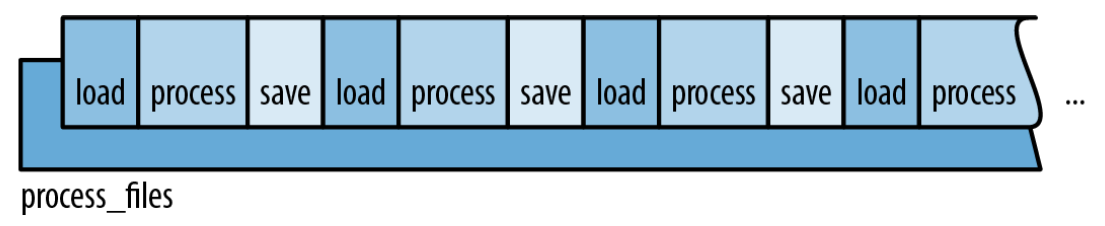
\includegraphics[width=0.9\textwidth]{../img/f19-1.png}
    \caption{单线程的\texttt{process\_files()}执行过程}
    \label{f19-1}
\end{figure}

因为每一个文档都是被单独处理,所以可以很容易的把所有文档分成几块、每一块在单独的线程中进行处理来加快速度,如\autoref{f19-2}所示。

\begin{figure}[htbp]
    \centering
    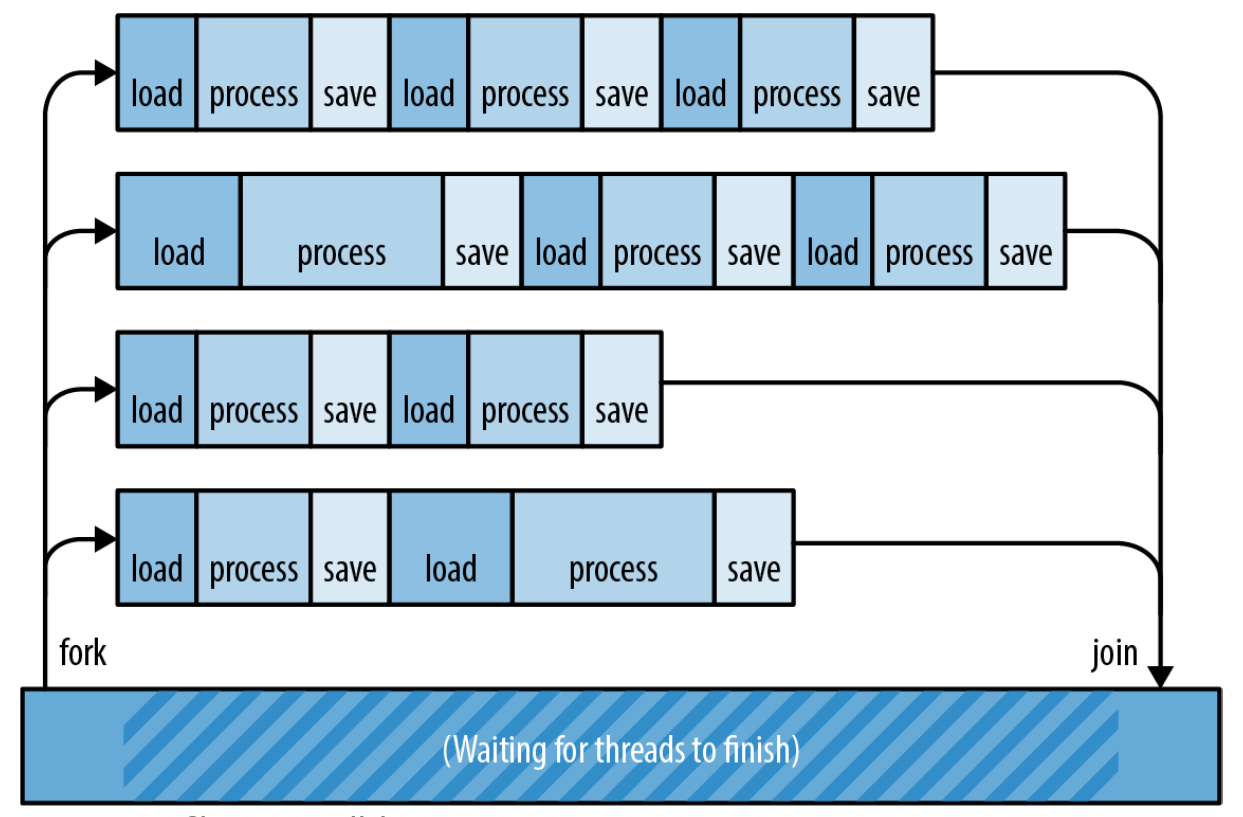
\includegraphics[width=0.8\textwidth]{../img/f19-2.png}
    \caption{使用fork-join方法的多线程文件处理}
    \label{f19-2}
\end{figure}

这个模式被称为\emph{fork-join并行}。\emph{fork}是启动一个新的线程,\emph{join}一个线程是等待它结束。我们已经看到过这个技术了:我们在\hyperref[ch02]{第2章}中使用了它来加速曼德勃罗集程序。

fork-join并行的优势主要在以下几个方面:
\begin{enumerate}
    \item 它太简单了。fork-join非常容易实现,并且Rust能帮你很轻松地保证它正确。
    \item 它避免了瓶颈。fork-join中没有共享资源的加锁。每个线程唯一要等待的时间就是最后要等待另一个线程结束。同时,每一个线程都可以自由地运行。这有助于保证很低的任务切换开销。
    \item 性能也非常直观。在最好的情况下,通过启动4个线程,我们可以用$\frac{1}{4}$的时间完成任务。\autoref{f19-2}展示了为什么我们不应该期待这种理想的加速:我们可能不能均匀地把工作分布到所有的线程上。另一个要注意的原因是一些fork-join程序在所有的线程结束之后还要花费一些时间\emph{组合(combine)}所有线程计算出的结果。即,完全分割任务可能要花费一些额外的工作。如果不考虑这两个原因,一个任务可以分割为独立单元的CPU密集的程序可以期待显著的性能提升。
    \item 很容易推断程序的正确性。只要每个线程真的被隔离,那么一个fork-join程序是\emph{确定性的(deterministic)},例如曼德勃罗集程序中的计算线程。程序总是会产生相同的结果,和线程速度的变化无关。它是一种没有竞争条件的并发模型。
\end{enumerate}

fork-join的主要缺点是它需要无关的任务单元。本章稍后我们会考虑一些不能分割的这么清晰的问题。

现在,让我们继续看自然语言处理的例子。我们将展示一些将fork-join模式应用于\texttt{process\_files}函数的方式。

\subsection{\texttt{spawn}和\texttt{join}}
函数\texttt{std::thread::spawn}启动一个新线程:
\begin{minted}{Rust}
    use std::thread;

    thread::spawn(|| {
        println!("hello from a child thread");
    });
\end{minted}

它接受一个参数:一个\texttt{FnOnce}闭包或者函数。Rust启动一个新的线程来运行这个闭包或者函数。新的线程是一个真实的操作系统线程,有自己的栈,就类似于C++、C\#、Java中的线程。

这里有一个例子,使用\texttt{spawn}来实现之前的\texttt{process\_files}函数的一个并行版本:
\begin{minted}{Rust}
    use std::{thread, io};

    fn process_files_in_parallel(filenames: Vec<String>) -> io::Result<()> {
        // 把工作分成几块。
        const NTHREADS: usize = 8;
        let worklists = split_vec_into_chunks(filenames, NTHREADS);

        // Fork:创建一个新线程来处理每一个块。
        let mut thread_handles = vec![];
        for worklist in worklists {
            thread_handles.push(
                thread::spawn(move || process_files(worklist))
            );
        }

        // Join:等待所有线程结束。
        for handle in thread_handles {
            handle.join().unwrap()?;
        }

        Ok(())
    }
\end{minted}

让我们逐行分析这个函数。
\begin{minted}{Rust}
    fn process_files_in_parallel(filenames: Vec<String>) -> io::Result<()> {
\end{minted}

我们的新函数和原本的\texttt{process\_files}有完全相同的类型签名,这让它可以更轻松地替换原来的函数。

\begin{minted}{Rust}
        // 把工作分成几块。
        const NTHREADS: usize = 8;
        let worklists = split_vec_into_chunks(filenames, NTHREADS);
\end{minted}

我们使用了一个工具函数\texttt{split\_vec\_into\_chunks}来分割任务,不过这里没有显示。分割的结果\texttt{worklists}是一个vector的vector。它包含原本的vector \texttt{filenames}均匀分配的8个部分。

\begin{minted}{Rust}
        // Fork:创建一个新线程来处理每一个块。
        let mut thread_handles = vec![];
        for worklist in worklists {
            thread_handles.push(
                thread::spawn(move || process_files(worklist))
            );
        }
\end{minted}

我们为每一个\texttt{worklist}启动了一个线程。\texttt{spawn()}返回一个称为\texttt{JoinHandle}的值,我们之后会使用它。现在,我们只是将所有的\texttt{JoinHandle}放进一个vector里。

注意我们如何把文件名的列表传进工作线程里:
\begin{enumerate}
    \item \texttt{worklist}在父线程的\texttt{for}循环中定义和初始化。
    \item 一旦\texttt{move}闭包创建完成,\texttt{worklist}就会被移动进闭包里
    \item 然后\texttt{spawn}把闭包(包括\texttt{worklist})移动进新的子线程。
\end{enumerate}

这些移动操作开销很小。正如我们在\hyperref[ch04]{第4章}中讨论的\texttt{Vec<String>}的移动一样,\texttt{String}并不会被拷贝。事实上,没有任何东西被分配或者释放。唯一被移动的数据是\texttt{Vec}自己:三个机器字。

你创建的大多数线程都同时需要代码和数据才能运行。Rust闭包可以便捷地包含了你需要的代码和数据。。

继续:
\begin{minted}{Rust}
        // Join:等待所有线程结束。
        for handle in thread_handles {
            handle.join().unwrap()?;
        }
\end{minted}

我们使用了之前收集的\texttt{JoinHandle}的\texttt{.join()}方法来等待8个线程全部结束。为了保证正确性,join线程通常是必须的,因为一旦\texttt{main}返回Rust程序就会退出,即使其他的线程仍然在运行。析构器不会被调用,额外的线程被简单地杀死。如果这不是你想要的,确保在\texttt{main}返回之前join所有你关心的线程。

如果这个循环结束了,那么意味着8个子线程都已经成功结束。我们的函数返回一个\texttt{Ok(())}并结束:
\begin{minted}{Rust}
        Ok(())
    }
\end{minted}

\subsection{跨线程的错误处理}

\section{channel}

\subsection{发送值}

\subsection{接收值}

\subsection{运行管道}

\subsection{通道的特性和性能}

\subsection{线程安全:\texttt{Send}和\texttt{Sync}}\label{threadsafe}

\section{共享可变状态}

\subsection{自旋锁是什么?}

\subsection{Mutex<T>}\label{mutex}

\subsection{mut和Mutex}

\subsection{为什么有时自旋锁不是好的方案}

\subsection{死锁}

\subsection{中毒的自旋锁}

\subsection{使用自旋锁的多消费者channel}

\subsection{读写锁(RwLock<T>)}

\subsection{条件变量(Condvar)}

\subsection{原子量}\label{atomic}

\subsection{全局变量}\label{globalvar}
    \chapter{异步编程}\label{ch20}

假设你正在编写一个聊天服务器。每个网络连接都有很多要解析的到来的包、要组装的发送的包、要管理的安全参数、要追踪的聊天组订阅等。同时为许多连接管理所有这些信息需要进行一些组织。

理想情况下,你可以简单地为每一个到来的连接启动一个单独的线程:
\begin{minted}{Rust}
    use std::{net, thread};

    let listener = net::TcpListener::bind(address)?;

    for socket_result in listener.incoming() {
        let socket = socket_result?;
        let groups = chat_group_table.clone();
        thread::spawn(|| {
            log_error(serve(socket, groups));
        });
    }
\end{minted}

这样对每一个连接都会创建一个新的线程运行\texttt{serve}函数,这个函数专门处理一个连接的需求。

这可以正常工作,直到一切都比计划的更加顺利很多,然后突然你就已经有了几万名用户。一个线程的栈增长到100KB或更多并不罕见,你可能不想就这样花费几GB的内存。要把任务分发到多个处理器上,线程是合适并且必须的,但它们的内存需求太大以至于我们通常需要一些补充的方式和线程一起使用,来减小资源占用。

你可以使用Rust的\emph{异步任务(asynchronous task)}来在单个线程或者线程池中交替执行很多独立的任务。异步任务类似于线程,但可以更快地创建、更高效地传递控制权、并且内存开销比线程少一个数量级。在单个程序中同时运行数十万个异步任务是完全可行的。当然,你的应用仍然可能被其他因素限制,例如网络带宽、数据库速度、计算、或者任务本身的内存需求,但使用异步任务的固有内存开销比使用线程的要小很多。

一般来讲,异步Rust代码看起来和普通的多线程代码非常相似,除了那些可能阻塞的操作,例如I/O或获取锁的处理有一点不同。特殊对待这些操作让Rust有更多的信息了解你的代码的行为,这为进一步优化提供了可能。上面代码的异步版本看起来像这样:
\begin{minted}{Rust}
    use async_std::{net, task};

    let listener = net::TcpListener::bind(address).await?;

    let mut new_connections = listener.incoming();
    while let Some(socket_result) = new_connections.next().await {
        let socket = socket_result?;
        let groups = chat_group_table.clone();
        task::spawn(async {
            log_error(serve(socket, groups).await);
        });
    }
\end{minted}

这里使用了\texttt{async\_std} crate的网络和任务模块,并在可能阻塞的调用后加上了\texttt{.await}。但整体的结构和基于线程的版本一样。

这一章的目标不止是帮你编写异步代码,还要向你展示它的工作细节,以便你可以预测它在你的应用中的表现,并了解它在哪些方面最有价值。

\begin{enumerate}
    \item 为了展示异步编程的机制,我们列出了涵盖所有核心概念的最小语言功能集:future、异步函数、\texttt{await}表达式、task、\texttt{block\_on}和\texttt{spawn\_local} executor。
    \item 然后我们会展示异步块和\texttt{spawn} executor。它们是完成真实工作的最基础的部分,但从概念上讲,它们只是我们刚才提到过的功能的变体。在这个过程中,我们会指出一些你可能会遇到的异步编程特有的问题并解释如何处理它们。
    \item 为了展示所有功能的协调工作,我们会展示一个聊天服务器和客户端的完整代码,上面的代码片段就是其中一部分。
    \item 为了演示原语future和executor如何工作,我们会展示\texttt{spawn\_blocking}和\texttt{block\_on}的简单实现。
    \item 最后,我们介绍了异步接口中经常出现的\texttt{Pin}类型,它被用来确保异步函数和块future被安全地使用。
\end{enumerate}

\section{从同步到异步}

考虑当你调用下面的(不是异步的)函数时会发生什么:
\begin{minted}{Rust}
    use std::io::prelude::*;
    use std::net;

    fn cheapo_request(host: &str, port: u16, path: &str)
                          -> std::io::Result<String>
    {
        let mut socket = net::TcpStream::connect((host, port))?;

        let request = format!("GET {} HTTP/1.1\r\nHost: {}\r\n\r\n", path, host);
        socket.write_all(request.as_bytes())?;
        socket.shutdown(net::Shutdown::Write)?;

        let mut response = String::new();
        socket.read_to_string(&mut response)?;

        Ok(response)
    }
\end{minted}

这会打开一个到web服务器的TCP连接,以过时的协议向它发送一个简单的HTTP请求,\footnote{如果你真的需要一个HTTP客户端,考虑使用一些非常优秀的crate例如\texttt{surf}或\texttt{reqwest},它们会正确并且异步地完成任务。这个客户端基本只是设法获得HTTPS重定向。}然后读取响应。\autoref{f20-1}展示了这个函数的执行过程随时间的变化。

\begin{figure}[htbp]
    \centering
    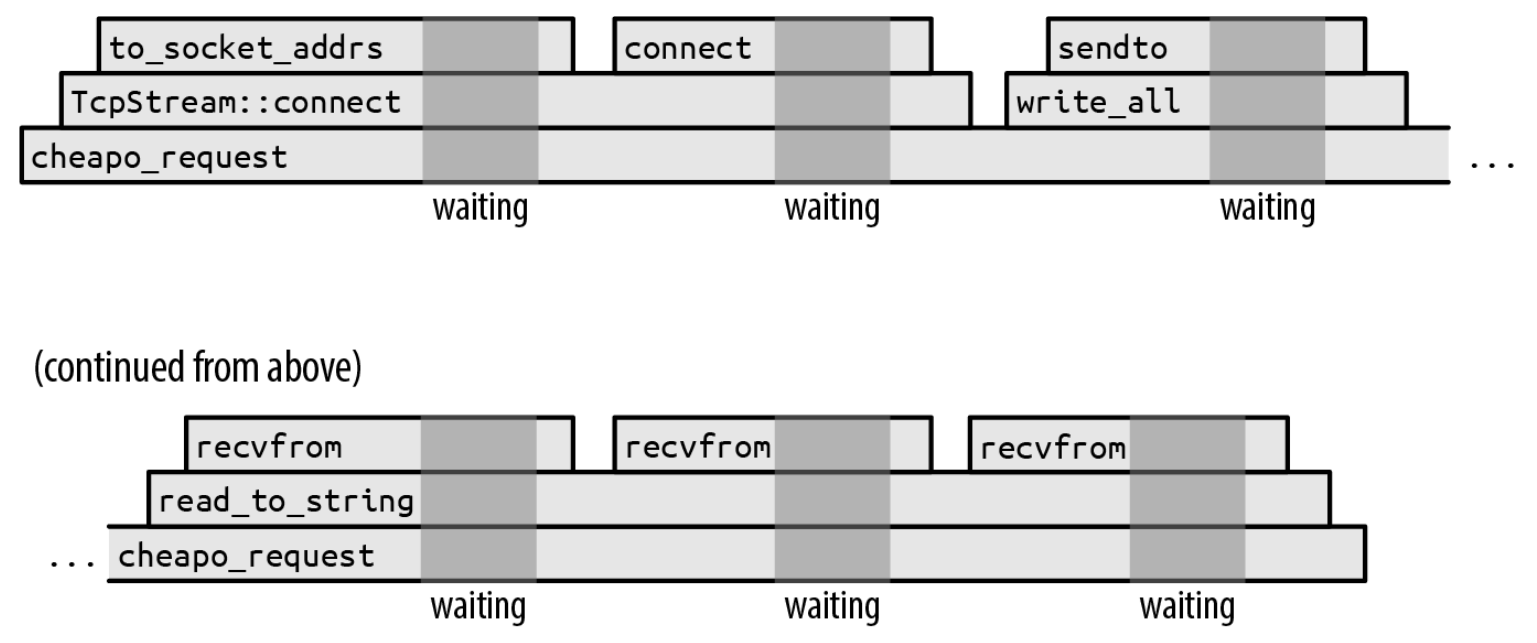
\includegraphics[width=0.8\textwidth]{../img/f20-1.png}
    \caption{一个同步HTTP请求的过程(深颜色的区域标识等待操作系统)}
    \label{f20-1}
\end{figure}

图中展示了从左到右随着时间的推移,函数的调用栈的变化。每一个函数调用都是一个方块,位于它的调用者上面。显然,\texttt{cheapo\_request}函数贯穿整个执行过程。它调用了Rust标准库里的函数例如\texttt{TcpStream::connect}和\texttt{TcpStream}的\texttt{write\_all}和\texttt{read\_to\_string}实现。这些对其他函数的调用依次进行,但最终程序会进行\emph{系统调用},请求操作系统完成真正的工作,例如打开TCP连接,或者读写一些数据。

深灰色的区域表示程序正在等待操作系统完成系统调用。我们并没有按比例绘制这些时间。因为加入我们按比例绘制,整个图都将是深灰色:在实践中,这个函数把几乎所有时间都用在等待操作系统上。上面代码的执行时间将是系统调用之间的窄条。

当函数等待系统调用返回时,它所在的线程会阻塞住:它不能做任何事,直到系统调用结束。一个线程的栈达到几百或几千字节并不罕见,因此如果这是一个更大的系统的一部分,并且有很多线程做类似的任务,锁住这些线程的资源但除了等待什么也不做的代价是非常昂贵的。

为了解决这个问题,一个线程需要能在等待系统调用完成的同时去执行其他的任务。但如何实现这一点并不明显。例如,我们用来从套接字读取响应的函数的签名是:
\begin{minted}{Rust}
    fn read_to_string(&mut self, buf: &mut String) -> std::io::Result<usize>;
\end{minted}

它的类型表明了:这个函数直到工作完成或者出错时才会返回。这个函数是\emph{同步的}:当操作完成时调用者才恢复。如果我们想在操作系统进行工作的同时用我们的线程去做别的任务,那么我们需要一个新的提供这个函数的\emph{异步}版本的I/O库。

\subsection{\texttt{Future}}
Rust支持异步操作的方法是引入一个trait:\texttt{std::future::Future}:
\begin{minted}{Rust}
    trait Future {
        type Output;
        // 现在,把`Pin<&mut Self>`看作`&mut Self`就好了。
        fn poll(self: Pin<&mut Self>, cx: &mut Context<'_>) -> Poll<Self::Output>;
    }

    enum Poll<T> {
        Ready(T),
        Pending,
    }
\end{minted}

一个\texttt{Future}代表一个可以测试是否完成的操作。一个future的\texttt{poll}方法从来不会等待操作完成:它总是立即返回。如果操作完成了,\texttt{poll}会返回\texttt{Poll::Ready(output)},其中\texttt{output}是最后的结果。否则,它会返回\texttt{Pending}。当且仅当future值得再次poll时,它会通过调用一个\emph{waker}来通知我们,这是一个由\texttt{Context}提供的回调函数。我们称之为异步编程的“piñata 模型” :你唯一能对future做的就是使用\texttt{poll}敲打它,直到有一个值掉出来。

所有现代的操作系统都包含一些系统调用的变体,我们可以用它们来实现这种poll接口。例如在Unix和Windows上,如果你把网络套接字设置为非阻塞模式,那么如果它们正在阻塞时进行read和write会返回错误,你必须稍后再试。

因此\texttt{read\_to\_string}的一个异步版本的签名大概是这样:
\begin{minted}{Rust}
    fn read_to_string(&mut self, buf: &mut String)
        -> impl Future<Output = Result<usize>;
\end{minted}

除了返回类型之外,这和我们之前展示的签名一样:异步的版本返回\emph{一个\texttt{Result<usize>}的future}。你需要poll这个future,直到从它得到一个\texttt{Ready(result)}。每次它被poll时,都会尽可能地继续读取。最后的\texttt{result}给你成功的值或者错误的值,就像普通的I/O操作一样。这是通常的模式:异步版本的任何函数和同步版本的函数获取相同的参数,但返回类型有一个\texttt{Future}包装。

调用这个版本的\texttt{read\_to\_string}并不会真的读取任何内容;它所有的任务就是构造并返回一个future,这个future会在被poll时进行真正的工作。这个future必须包含处理请求所需的所有信息。例如,这个\texttt{read\_to\_string}返回的future必须记住调用它的输入流,和它需要写入数据的\texttt{String}。事实上,因为这个future持有了\texttt{self}和\texttt{buf}的引用,因此这个\texttt{read\_to\_string}的真正的签名必须是:
\begin{minted}{Rust}
    fn read_to_string<'a>(&'a mut self, buf: &'a mut String)
        -> impl Future<Output = Result<usize>> + 'a;
\end{minted}

这个附加的生命周期指示了返回的future和它借用的\texttt{self}和\texttt{buf}的生命周期一样长。

\texttt{async-std} crate提供了\texttt{std}的所有I/O设施的异步版本,包括一个有\texttt{read\_to\_string}方法的异步\texttt{Read} trait。\texttt{async-std}密切地遵循了\texttt{std}的设计,尽可能地在自己的接口中重用\texttt{std}的类型,因此这两个世界中的错误、结果、网络地址、和其他大多数相关的数据都是兼容的。熟悉\texttt{std}有助于使用\texttt{async-std},反之亦然。

\texttt{Future} trait的一个规则是,一旦一个future返回了\texttt{Poll::Ready},它会假设它决不会再次被poll。一些future在自己被overpoll时简单地永远返回\texttt{Poll::Pending};其它的可能panic或者挂起。(它们绝不能违反内存或线程安全性,或者导致未定义行为)\texttt{Future} trait的\texttt{fuse}适配器将任何future转换成overpoll时永远返回\texttt{Poll::Pending}。但通常消费future的方法都遵循这个规则,因此\texttt{fuse}通常不是必须的。

如果poll听起来效率底下,请不必担心。Rust的异步架构是精心设计的,所以只要你的基本I/O函数例如\texttt{read\_to\_string}是正确实现的,那么你只会在值的时poll一个future。每一次\texttt{poll}被调用时,某个东西应该返回\texttt{Ready},或者至少向目标前进一步。我们将在“\nameref{WhenPoll}”中解释这是如何工作的。

但使用future看起来有一个挑战:当你poll时,如果你得到了\texttt{Poll::Pending}那你应该怎么做?你将不得不四处寻找这个线程暂时可以做的其他工作,并记住一段时间之后返回到这个future,然后再次poll。你的整个系统将因为持续追踪谁正在pending和当它们完成时应该做什么而变得杂乱无章。我们的\texttt{cheapo\_request}函数的简洁性会被破坏。

好消息是:它并不是这样的!

\subsection{\texttt{async}函数和\texttt{await}表达式}
这里有一个\emph{异步函数}版本的\texttt{cheapo\_request}:
\begin{minted}{Rust}
    use async_std::io::prelude::*;
    use async_std::net;

    async fn cheapo_request(host: &str, port: u16, path: &str)
                                -> std::io::Result<String>
    {
        let mut socket = net::TcpStream::connect((host, port)).await?;

        let request = format!("GET {} HTTP/1.1\r\nHost: {}\r\n\r\n", path, host);
        socket.write_all(request.as_bytes()).await?;
        socket.shutdown(net::Shutdown::Write)?;

        let mut response = String::new();
        socket.read_to_string(&mut response).await?;

        Ok(response)
    }
\end{minted}

这和之前的版本基本相同,除了:
\begin{enumerate}
    \item 函数以\texttt{async}代替\texttt{fn}开头。
    \item 它使用了\texttt{async\_std} crate里的异步版本的\texttt{TcpStream::connect, write\_all, read\_to\_string}。它们都返回结果的future(本节中的示例使用了\texttt{async\_std}的1.7版本)。
    \item 每一次调用返回future的函数之后,代码都会加上\texttt{.await}。尽管这看起来像是访问一个结构体的\texttt{await}字段,但它实际上是语言内置的一个特殊语法,它会等待一个future直到它准备好。\texttt{await}表达式会求出future的最终值。这个函数正是通过它获取\texttt{connect, write\_all, read\_to\_string}的结果。
\end{enumerate}

和普通的函数不同,当你调用异步函数时,它会在执行实际的主体代码之前立即返回。显然,调用的返回值还没有被计算出来;你得到的是它的最终值的\emph{future}。因此如果你执行这行代码:
\begin{minted}{Rust}
    let response = cheapo_request(host, port, path);
\end{minted}

那么\texttt{response}将是一个\texttt{std::io::Result<String>}的future,\texttt{cheapo\_request}的函数体还没有开始执行。你不需要调整异步函数的返回类型;Rust会自动把\texttt{async fn f(...) -> T}看做一个返回\texttt{T}的future而不是直接返回\texttt{T}的函数。

一个异步函数返回的future包含了函数体运行时所需的所有信息:函数的参数、局部变量所需的空间,等等。(就好像你把调用栈捕获为了一个普通的Rust值。)因此\texttt{response}必须包含传入的\texttt{host, port, path},因为\texttt{cheapo\_request}的函数体需要它们才能运行。

future的具体类型由编译器根据函数体和参数自动生成。这个类型并没有名称;你只知道它实现了\texttt{Future<Output=R>},其中\texttt{R}是异步函数的返回类型。从这一点来看,异步函数的future类似于闭包:闭包也有匿名类型、也是由编译器生成并且实现了\texttt{FnOnce}、\texttt{Fn}和\texttt{FnMut} trait。

当你第一次poll \texttt{cheapo\_request}返回的future时,将会从函数体的尾部开始运行到第一个由\texttt{TcpStream::connect}返回的future的\texttt{await}。这个\texttt{await}表达式会poll \texttt{connect} future,如果它还没准备好,那么它会向调用者返回\texttt{Poll::Pending}:直到\texttt{TcpStream::connect}的future返回\texttt{Poll::Ready}时,对\texttt{cheapo\_request}的future的poll才能继续通过第一个\texttt{await}。因此表达式\texttt{TcpStream::connect(...).await}的一个大概等价的写法是:
\begin{minted}{Rust}
    {
        // 注意:这是伪代码,不是有效的Rust代码
        let connect_future = TcpStream::connect(...);
        'retry_point:
        match connect_future.poll(cx) {
            Poll::Ready(value) => value,
            Poll::Pending => {
                // 设置`cheapo_request`的future的下一次`poll`
                // 从'retry_point处恢复执行。
                ...
                return Poll::Pending
            }
        }
    }
\end{minted}

一个\texttt{await}表达式会获取future的所有权然后poll它。如果它已经准备好,那么future的最终值就是\texttt{await}表达式的值,并且会继续往下执行。否则,它向调用者返回\texttt{Poll::Pending}。

但关键的是,下一次poll \texttt{cheapo\_request}的future时将不会再次从函数的首部开始:相反,它从poll \texttt{connect\_future}的地方开始\emph{恢复(resume)}执行。直到future准备好之后我们才会继续执行这个异步函数的其他部分。

随着\texttt{cheapo\_request}的future继续被poll,它会从函数体里的一个\texttt{await}开始执行到下一个,只有当它正在等待的子future ready时才会继续。因此,\texttt{cheapo\_request}的future将会被poll多少次取决于子future的行为和函数本身的控制流。\texttt{cheapo\_request}的future会追踪下一次\texttt{poll}时的恢复点和所有的局部状态——变量、参数、临时值——恢复需要这些。

在函数中间挂起并稍后恢复执行的能力是异步函数独有的。当普通函数返回时,它的栈帧就消失了。因为\texttt{await}表达式依赖于恢复执行的能力,所以你只能在异步函数里使用它们。

在撰写本书时,Rust还不允许trait有异步方法。只有自由函数和特定类型固有的方法才可以是异步的。取消这个限制需要对语言进行一些修改。与此同时,如果你需要定义包含异步函数的trait,可以考虑使用\texttt{async-trait} crate,它提供了一个基于宏的解决方案。

\subsection{在同步代码中调用异步函数:\texttt{block\_on}}
某种意义上讲,异步函数只是在推卸责任。在异步函数里很容易获取一个future的值:只需要\texttt{await}它。但异步函数\emph{本身}也返回一个future,因此现在调用者需要负责poll它。最后,总有一个地方必须实际等待一个值。

我们可以使用\texttt{async\_std}的\texttt{task::block\_on}函数在普通的同步函数(例如\texttt{main})中调用\texttt{cheapo\_request},它获取一个future并且poll它直到它产生一个值:
\begin{minted}{Rust}
    fn main() -> std::io::Result<()> {
        use async_std::task;

        let response = task::block_on(cheapo_request("example.com", 80, "/))?;
        println!("{}", response);
        Ok(())
    }
\end{minted}

因为\texttt{block\_on}是一个产生异步函数的最终值的同步函数,你可以将它看作是异步世界到同步世界的适配器。但它阻塞的特性也意味着你永远不应该在一个异步函数里使用\texttt{block\_on}:它会阻塞整个线程直到值准备好。作为代替,请使用\texttt{await}。

\autoref{f20-2}展示了\texttt{main}的一个可能的执行过程。

\begin{figure}[htbp]
    \centering
    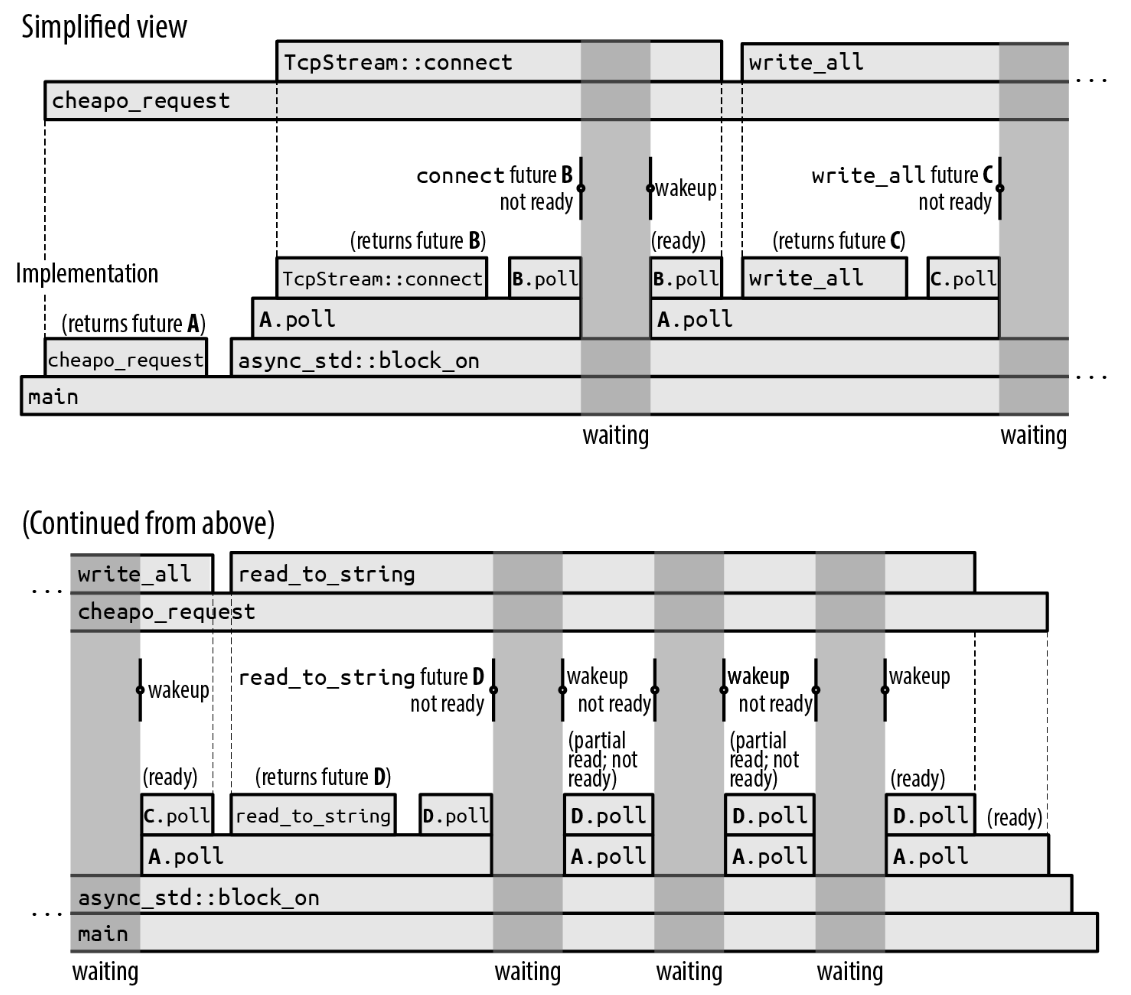
\includegraphics[width=0.9\textwidth]{../img/f20-2.png}
    \caption{阻塞等待一个异步函数}
    \label{f20-2}
\end{figure}

上面的时间线,“简化视图”,展示了程序的异步调用的抽象视图:\texttt{cheapo\_request}首先调用了\texttt{TcpStream::connect}来获取一个套接字,然后对套接字调用了\texttt{write\_all}和\texttt{read\_to\_string}。然后它返回。这和本章前面的同步版本的\texttt{cheapo\_request}的时间线非常相似。

但这里每一个异步调用都是多阶段的过程:一个future被创建,然后被poll直到它准备好,可能还会创建并poll其他子future。下面的时间线,“实现”,展示了实现了这个异步行为的实际同步调用。这是一个介绍普通的异步执行过程中到底发生了什么的好机会:
\begin{enumerate}
    \item 首先,\texttt{main}调用\texttt{cheapo\_request},它返回最终结果的future \texttt{A}。然后\texttt{main}把这个future传给了\texttt{async\_std::block\_on},它会poll \texttt{A}。
    \item poll future \texttt{A}允许\texttt{cheapo\_request}的函数体开始执行。函数里调用了\texttt{TcpStream::connect}来获取一个套接字的future \texttt{B}并await它。更确切地说,因为\texttt{TcpStream::connect}可能会遇到错误,因此\texttt{B}是一个\texttt{Result<TcpStream, std::io::Error}的future。
    \item future \texttt{B}被\texttt{await} poll。因为网络连接还没有建立好,所以\texttt{B.poll}返回\texttt{Poll::Pending},但会设置好当套接字准备好后唤醒调用它的任务。
    \item 因为future \texttt{B}还没有准备好,\texttt{A.poll}也会向它的调用者\texttt{block\_on}返回\texttt{Poll::Pending}。
    \item 因为\texttt{block\_on}没有别的事情可做,它会陷入睡眠。这时整个线程会阻塞。
    \item 当\texttt{B}的连接准备好之后,它会唤醒poll它的任务。这促使\texttt{block\_on}开始行动,它会尝试再次poll future \texttt{A}。
    \item poll \texttt{A}促使\texttt{cheapo\_request}在它的第一个\texttt{await}处恢复执行,然后再次poll \texttt{B}。
    \item 这一次,\texttt{B}准备好了:套接字已经创建完毕,因此它返回\texttt{Poll::Ready(Ok(socket))}到\texttt{A.poll}。
    \item 到此\texttt{TcpStream::connect}的异步调用就完成了。\texttt{TcpStream::connect(...).await}表达式的值就是\texttt{Ok(socket)}。
    \item \texttt{cheapo\_request}的函数体会继续正常执行,使用\texttt{format!}宏构造请求字符串并传递给\texttt{socket.write\_all}。
    \item 因为\texttt{socket.write\_all}是一个异步函数,它会返回一个future \texttt{C},\texttt{cheapo\_request}会await \texttt{C}。
\end{enumerate}

剩余的流程和之前相似。在\autoref{f20-2}所示的执行流程中,\texttt{socket.read\_to\_string}在准备好之前被poll了四次,每一次都会从套接字读取\emph{一些}数据,但\texttt{read\_to\_string}被指定为一直读取到输入的末尾,这需要好几次的操作。

听起来编写一个一直调用\texttt{poll}的循环并不难。但让\texttt{async\_std::task::block\_on}真正有价值的是:它知道怎么睡眠到恰好future值得再次poll,而不是浪费处理器的时间和电量来进行几十亿次无用的\texttt{poll}调用。基本的I/O函数例如\texttt{connect}和\texttt{read\_to\_string}返回的future保留了传递给\texttt{poll}的\texttt{Context}参数提供的唤醒器,并在\texttt{block\_on}应该醒来并再次尝试poll时调用唤醒器。我们将在“\nameref{WhenPoll}”中通过实现一个简单版本的\texttt{block\_on}来展示这具体是怎么工作的。

和我们之前展示的原始的同步版本一样,这个异步版本的\texttt{cheapo\_request}方法也把几乎所有的时间花费在等待操作完成上。如果时间轴是按比例绘制的,那么图将几乎完全是深灰色的,只有当程序被唤醒时会有几个计算过程对应的很细的条。

这里讲了很多细节。幸运的是,你通常可以只考虑简化的上层时间线:一些函数调用是同步的,其他是异步的并需要一个\texttt{await},但它们都只是函数调用。Rust的异步支持的成功取决于帮助程序员在实践中只需要考虑简化的视图,不会被实现的来回跳转干扰。

\subsection{spawn异步任务}
\texttt{async\_std::task::block\_on}函数会阻塞知道一个future的值准备好。但在单个future上完全阻塞一个线程并不比同步调用更好:本章的目的是让线程在等待的同时\emph{做别的工作}。

为了实现这一点,你可以使用\texttt{async\_std::task::spawn\_local}。这个函数接受一个future并把它添加到一个池,当\texttt{block\_on}阻塞等待的future还没准备好时\texttt{block\_on}会poll这个池。因此如果你把一堆future传递给\texttt{spawn\_local}并且之后对最终结果的future调用\texttt{block\_on},\texttt{block\_on}会poll每一个被spawn的future(当它们可以进一步执行时),并发运行整个池,直到结果准备好。

在撰写本书时,只有当你启用\texttt{async-std} crate的\texttt{unstable}特性时\texttt{spawn\_local}才可用。你需要在\emph{Cargo.toml}中用这样的一行引入\texttt{async-std}:
\begin{minted}{toml}
    async-std = { version = "1", features = ["unstable"] }
\end{minted}

\texttt{spawn\_local}函数是标准中用于启动新线程的\texttt{std::thread::spawn}函数的异步版本的类似物:
\begin{enumerate}
    \item \texttt{std::thread::spawn(c)}接收闭包\texttt{c}然后启动一个线程运行它,返回一个\texttt{std::thread::JoinHandle},它的\texttt{join}方法会等待线程结束并返回\texttt{c}返回的内容。
    \item \texttt{async\_std::task::spawn\_local(f)}接收future \texttt{f}并把它添加到当前线程调用\texttt{block\_on}时会poll的池里。\texttt{spawn\_local}会返回它自己的\texttt{async\_std::task::JoinHandle}类型,它本身是一个future,你可以await它来获取\texttt{f}的最终值。
\end{enumerate}

例如,假设我们想让一个HTTP请求的集合并发执行。这是第一次尝试:
\begin{minted}{Rust}
    pub async fn many_requests(requests: Vec<(String, u16, String)>)
                               -> Vec<std::io::Result<String>>
    {
        use async_std::task;

        let mut handles = vec![];
        for (host, port, path) in requests {
            handles.push(task::spawn_local(cheapo_request(&host, port, &path)));
        }

        let mut results = vec![];
        for handle in handles {
            results.push(handle.await);
        }

        results
    }
\end{minted}

这个函数对\texttt{requests}的每个元素调用\texttt{cheapo\_request},将每一个调用返回的future传给\texttt{spawn\_local}。它把最后的\texttt{JoinHandle}收集到一个vector并且await每一个。以任意顺序await join handles都是没问题的:因为请求已经被spawn,它们的future将会被按需poll,即这个线程调用了\texttt{block\_on}并且无事可做时。所有的请求会并发运行。一旦它们完成,\texttt{many\_requests}会向调用者返回结果。

上面的代码几乎是正确的,但Rust的借用检查器担心\texttt{cheapo\_request}的future的生命周期:
\begin{minted}{text}
    error: `host` does not live long enough
        handles.push(task::spawn_local(cheapo_request(&host, port, &path)));
                                       ---------------^^^^^-------------
                                       |              |
                                       |              borrowed value does not
                                       |              live long enough
                         argument requires that `host` is borrowed for `'static`
    }
    - `host` dropped here while still borrowed
\end{minted}

\texttt{path}也有一个类似的错误。

自然地,如果我们向异步函数传递引用,那么它们返回的future就必须持有这些引用,因此出于安全性future不能比它们借用的值生存的更久。任何持有引用的其他值也有相同的限制。

问题在于\texttt{spawn\_local}不能确保你会在\texttt{host}和\texttt{path}被drop之前等待任务结束。事实上,\texttt{spawn\_local}只接受生命周期是\texttt{'static}的future,因为你可以简单地忽略它返回的\texttt{JoinHandle}并让任务在程序的剩余部分执行时继续运行。这并不是异步任务独有的问题:当你尝试用\texttt{std::thread::spawn}启动一个线程,并且它的闭包捕获了局部变量的引用时也会遇到类似的错误。

一种解决这个问题的方法是创建另一个版本的获取参数所有权的异步函数:
\begin{minted}{Rust}
    async fn cheapo_owning_request(host: String, port: u16, path: String)
                                   -> std::io::Result<String> {
        cheapo_request(&host, port, &path).await
    }
\end{minted}

这个函数接收\texttt{String}而不是\texttt{\&str}引用,因此它的future自身将拥有\texttt{host}和\texttt{path},并且生命周期是\texttt{'static}。借用检查器可以看到它立刻await了\texttt{cheapo\_request}的future,并且因此如果这个future被poll,它借用的\texttt{host}和\texttt{path}变量肯定还在。一切都没有问题。

使用\texttt{cheapo\_owning\_request},你可以像这样spwan所有的请求:
\begin{minted}{Rust}
    for (host, port, path) in requests {
        handles.push(task::spawn_local(cheapo_owning_request(host, port, path)));
    }
\end{minted}

你可以使用\texttt{block\_on}在同步的\texttt{main}函数中调用\texttt{many\_requests}:
\begin{minted}{Rust}
    let requests = vec![
        ("example.com".to_string(),      80, "/".to_string()),
        ("www.red-bean.com".to_string(), 80, "/".to_string()),
        ("en.wikipedia.org".to_string(), 80, "/".to_string()),
    ];

    let results = async_std::task::block_on(many_requests(requests));
    for result in results {
        match result {
            Ok(response) => println!("{}", response),
            Err(err) => eprintln!("error: {}", err),
        }
    }
\end{minted}

这段代码会在\texttt{block\_on}的调用中并发运行三个请求。每个请求会在当其他的请求阻塞时抓住几乎继续执行,它们全部在调用者线程中执行。\autoref{f20-3}中展示了三个\texttt{cheapo\_request}调用的可能的执行过程。

\begin{figure}[htbp]
    \centering
    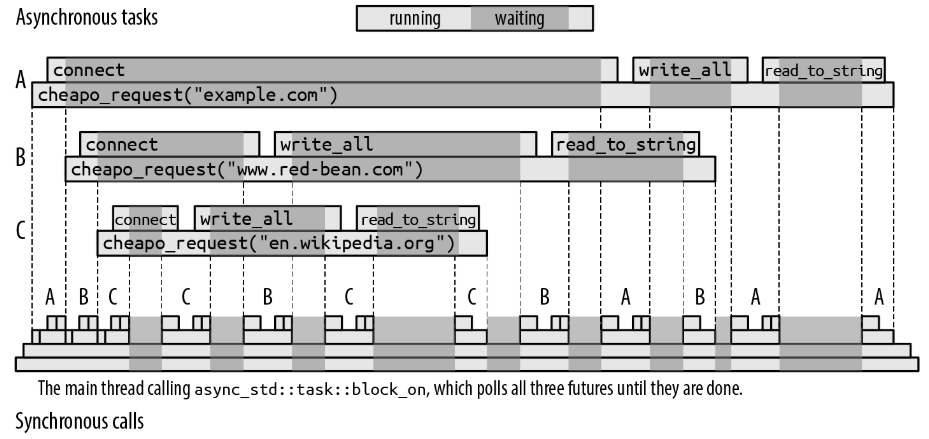
\includegraphics[width=0.9\textwidth]{../img/f20-3.png}
    \caption{在单个线程中运行三个异步任务}
    \label{f20-3}
\end{figure}

(我们鼓励你自己尝试运行这段代码,使用\texttt{eprintln!}在\texttt{cheapo\_request}首部和每一个\texttt{await}表达式之后打印消息,这样你可以看到这些调用如何交错执行。)

对\texttt{many\_requests}的调用(为了简单没有展示)spawn了三个异步的任务,分别用\texttt{A}、\texttt{B}、\texttt{C}标记。\texttt{block\_on}开始时先poll \texttt{A},\texttt{A}会开始连接到\texttt{example.com}。这会立刻返回\texttt{Poll::Pending},\texttt{block\_on}会把注意移动到下一个spawn的任务,然后poll future \texttt{B},最后是\texttt{C},它们会开始连接各自的服务器。

当所有可以poll的future都返回了\texttt{Poll::Pending}之后,\texttt{block\_on}会进入睡眠,直到其中一个\texttt{TcpStream::connect} future指示它的任务值得再次poll。

在这次执行中,服务器\texttt{en.wikipedia.org}比其他的响应得更快,因此这个任务最先完成。当一个spawn的任务完成时,它会把值保存在\texttt{JoinHandle}并标记它已经准备好了,这样\texttt{many\_requests} await它时无需等待,可以继续执行。最后,其它的\texttt{cheapo\_request}要么成功要么返回错误,然后\texttt{many\_request}本身可以返回了。最后,\texttt{main}接收\texttt{block\_on}返回的结果的vector。

所有这些执行都发生在单个线程中,三个\texttt{cheapo\_request}的调用通过对future的poll实现交错执行。一个异步调用看起来像是一个运行到完成的单个函数调用,但实际上异步调用由一系列对future的\texttt{poll}方法的同步调用实现。每一个单独的\texttt{poll}调用都可以快速返回,让出线程从而让其他异步调用可以执行。

我们终于达成了我们在本章开头设置的目标:让一个线程在等待I/O完成的同时去执行其他的工作,这样线程的资源不会因等待而浪费。更妙的是,达成这个目标的代码看起来非常像普通的Rust代码:一些函数被标记为\texttt{async}、一些函数调用后面有\texttt{.await}、使用的函数来自\texttt{async\_std}而不是\texttt{std},但除此之外,它就是普通的Rust代码。

异步任务和线程有一个不同之处需要牢记:异步任务只有在\texttt{await}表达式处被await的future返回\texttt{Poll::Pending}时才会切换到另一个异步任务。这意味着如果你在\texttt{cheapo\_request}中放了一段长时间运行的计算代码,那么在它完成之前,任何传给\texttt{spawn\_local}的其他任务都没有机会运行。而使用线程时没有这个问题:操作系统可以在任何地方挂起任何线程并设置计时器来确保没有线程可以垄断处理器。

异步代码依赖于共享线程的future的协作。如果你需要让长时间计算和异步代码共存,本章后面的“\nameref{LongCompute}”中介绍了一些方法。

\subsection{\texttt{async}块}
除了异步函数之外,Rust还支持\emph{异步块(asynchronous block)}。与一个普通的快块返回最后一个表达式的值不同,一个异步块返回最后一个表达式的\emph{值的future}。你可以在异步块里使用\texttt{await}表达式。

异步块看起来就像普通的块表达式,在前边加上\texttt{async}关键字:
\begin{minted}{Rust}
    let serve_one = async {
        use async_std::net;

        // 监听连接并接受
        let listener = net::TcpListener::bind("localhost:8087").await?;
        let (mut socket, _add) = listener.accept().await?;

        // 通过`socket`与客户端交互
        ...
    };
\end{minted}

这里用一个future初始化了\texttt{serve\_one},当poll它时,它会监听并处理单个TCP连接。块的代码直到\texttt{serve\_one}被poll才会执行,就像异步函数只有在它的future被poll时才会执行一样。

如果你在异步块里使用了\texttt{?}操作符,它会从块里返回,而不是从所处的函数返回。例如,如果上面的\texttt{bind}调用返回一个错误,那么\texttt{?}操作符会返回它作为\texttt{serve\_one}的最终值。类似的,\texttt{return}表达式会从异步块里返回,而不是从外层的函数返回。

如果一个异步块引用了周围代码里的变量,它的future会捕获那些变量,就像闭包一样。并且和\texttt{move}闭包一样(见“\nameref{StealClosure}”),你可以以\texttt{async move}来创建获取变量所有权的块,而不是持有变量的引用。

异步块提供了一种精确的分离出想要异步运行的部分代码的方法。例如,在上一节中,\texttt{spawn\_local}需要\texttt{'static} future,因此我们定义了\texttt{cheapo\_owning\_request}包装函数来得到一个获取参数所有权的future。你可以简单地在一个异步块里调用\texttt{cheapo\_request}而不需要分离出包装函数来实现相同的效果:
\begin{minted}{Rust}
    pub async fn many_requests(requests: Vec<(String, u16, String)>)
                               -> Vec<std::io::Result<String>>
    {
        use async_std::task;

        let mut handles = vec![];
        for (host, port, path) in requests {
            handles.push(task::spawn_local(async move {
                cheapo_request(&host, port, &path).await
            }));
        }
        ...
    }
\end{minted}

因为这是一个\texttt{async move}块,所以它的future获取了\texttt{String}值\texttt{host}和\texttt{path}的所有权,就类似\texttt{move}闭包一样。然后它向\texttt{cheapo\_request}传递引用,借用检查器可以看到块的\texttt{await}表达式获取了\texttt{cheapo\_request}的future的所有权,因此\texttt{host}和\texttt{path}的引用不可能比它们借用的被捕获的变量生存的更久。异步块和\texttt{cheapo\_owning\_request}完成了同样的事,但所需的样板代码更少。

一个你可能遇到的问题是没有语法能指定异步块的返回类型,即异步函数参数后跟的\texttt{-> T}。当使用\texttt{?}操作符时这可能会导致问题:
\begin{minted}{Rust}
    let input = async_std::io::stdin();
    let future = async {
        let mut line = String::new();

        // 这会返回`std::io::Result<usize>`。
        input.read_line(&mut line).await?;

        println!("Read line: {}", line);

        Ok(())
    };
\end{minted}

这会因为如下错误失败:
\begin{minted}{text}
    error: type annotations needed
       |
    42 |     let future = async {
       |         ------ consider giving `future` a type
    ...
    46 |         input.read_line(&mut line).await?;
       |         ^^^^^^^^^^^^^^^^^^^^^^^^^^^^^^^^^ cannot infer type
\end{minted}

Rust不能分辨异步块的返回类型应该是什么。\texttt{read\_line}方法返回\texttt{Result<(), std::io::Error>},但因为\texttt{?}操作符使用了\texttt{From} trait来在需要时转换成指定的错误类型,所以这个异步块的返回类型是\texttt{Result<(), E>},其中\texttt{E}可能是任何实现了\texttt{From<std::io::Error>}的类型。

Rust未来的版本可能会添加指定\texttt{async}块的返回类型的语法。但现在,可以通过手动写出最后的\texttt{Ok}的类型来解决这个问题:
\begin{minted}{Rust}
    let future = async {
        ...
        Ok::<(), std::io::Error>(())
    };
\end{minted}

因为\texttt{Result}是一个需要成功和错误类型作为参数的泛型类型,我们可以像这里一样使用\texttt{Ok}或\texttt{Err}指定那些类型参数。

\subsection{从异步块中构建异步函数}
异步块给了我们另一种实现和异步函数相同效果的方法,并且更加灵活一点。例如,我们可以将我们的\texttt{cheapo\_request}写成一个普通的、同步的返回异步块的future的函数:
\begin{minted}{Rust}
    use std::io;
    use std::future::Future;

    fn cheapo_request<'a>(host: &'a str, port: u16, path: &'a str)
        -> impl Future<Output = io::Result<String>> + 'a
    {
        async move {
            ... function body ...
        }
    }
\end{minted}

当你调用这个版本的函数时,它会立刻返回异步块的值的future。这个future会捕获函数的参数并且和异步函数返回的future的行为一样。因为我们没有使用\texttt{async fn}语法,我们需要在返回值中写出\texttt{impl Future},但对调用者来说,这两个定义是同一个函数签名的两种可替换的实现。

如果你想让函数被调用时立刻进行一些计算然后再构造返回的future,那么第二种方法更有用。例如,另一种协调\texttt{cheapo\_request}和\texttt{spawn\_local}的方法是让它变成一个返回\texttt{'static} future的同步函数,并让这个future捕获参数的拷贝的所有权:
\begin{minted}{Rust}
    fn cheapo_request(host: &str, port: u16, path: &str)    
        -> impl Future<Output = io::Result<String> + 'static
    {
        let host = host.to_string();
        let path = path.to_string();

        async move {
            ... use &*host, port, and path ...
        }
    }
\end{minted}

这个版本让异步块捕获\texttt{host}和\texttt{path}为\texttt{String}值,而不是\texttt{\&str}引用。因为future拥有自己运行所需的所有数据,所以它是有效的\texttt{'static}生命周期。(我们在上面的签名中写出了\texttt{+ 'static},但\texttt{-> impl}返回的类型默认是\texttt{'static}的,因此省略它不会有影响。)

因为这个版本的\texttt{cheapo\_request}返回的future是\texttt{'static}的,我们可以直接把它们传递给\texttt{spawn\_local}:
\begin{minted}{Rust}
    let join_handle = async_std::task::spawn_local(
        cheapo_request("areweasyncyet.rs", 80, "/")
    );

    ... other work ...

    let response = join_handle.await?;
\end{minted}

\subsection{在一个线程池中spawn异步任务}
我们至今为止展示过的例子几乎把所有时间花费在等待I/O上,但一些负载是更多处理器工作和阻塞的组合。当你有太多的计算以至于单个处理器不能进行快速处理,你可以使用\texttt{async\_std::task::spawn}来把一个future spawn到一个工作线程池里,这些线程会poll可以进一步执行的future。

\texttt{async\_std::task::spawn}的使用方法类似\texttt{async\_std::task::spawn\_local}:
\begin{minted}{Rust}
    use async_std::task;

    let mut handles = vec![];
    for (host, port, path) in requests {
        handles.push(task::spawn(async move {
            cheapo_request(&host, port, &path).await
        }));
    }
    ...
\end{minted}

类似于\texttt{spawn\_local},\texttt{spawn}也返回一个\texttt{JoinHandle}值,你可以await它来获取future的最终值。但和\texttt{spawn\_local}不同的是,这个future不会等到你调用\texttt{block\_on}才会被poll,只要线程池中有一个空闲的线程,它就会尝试poll这个future。

在实践中,\texttt{spawn}比\texttt{spawn\_local}使用得更加广泛,因为人们更希望他们的负载不管计算和阻塞怎么混合,都能在机器上均衡地执行。

当使用\texttt{spawn}时一个需要记住的点是线程池会尝试保持忙碌,因此只要有一个线程空闲你的future就会被poll。一个异步调用可能在一个线程中开始执行,在一个\texttt{await}表达式处阻塞,最后在另一个不同的线程中恢复执行。因此将一个异步函数调用看作单个函数调用是一个合理的简化(事实上,异步函数和\texttt{await}表达式的目的就是鼓励你以这种方式思考)。和代码的执行情况有关,异步调用可能实际上会在很多不同线程中移动。

如果你正在使用thread-local存储,你可能会惊讶地发现你在\texttt{await}表达式之前放置的一些数据在恢复之后被替换成了某些完全不同的东西,这是因为你的任务现在正在被池中的另一个线程poll。如果这导致了问题,你应该使用\emph{task-local storage};细节见\texttt{async-std} crate中\texttt{task\_local!}宏的文档。

\subsection{但你的Future实现了\texttt{Send}吗?}
有一个\texttt{spawn}要求但\texttt{spawn\_local}不要求的限制。因为future被送到另一个线程运行,因此future必须实现了\texttt{Send}标记trait。我们在“\nameref{threadsafe}”中介绍过\texttt{Send}。只有当future包含的所有值都是\texttt{Send}时future才是\texttt{Send}:所有的函数参数、局部变量、甚至匿名的临时值都必须能安全地移动到另一个线程。

和之前一样,这个要求也不是异步任务独有的:如果你尝试使用\texttt{std::thread::spawn}启动一个捕获了非\texttt{Send}值的闭包也会遇到一个类似的错误。不同之处在于,传给\texttt{std::thread::spawn}的闭包会留在新创建的线程中运行,而spawn到线程池里的future可能会在await时从一个线程移动到另一个线程。

这个限制很容易意外触发。例如,下面的代码看起来足够合法:
\begin{minted}{Rust}
    use async_std::task;
    use std::rc::Rc;

    async fn reluctant() -> String {
        let string = Rc::new("ref-counted String".to_string());

        some_asynchronous_thing().await;

        format!("Your splendid string: {}", string)
    }

    task::spawn(reluctant());
\end{minted}

一个异步函数的future必须持有足够的信息来让它可以从一个\texttt{await}表达式继续执行。在这个例子中,\texttt{reluctant}的future必须在\texttt{await}之后使用\texttt{string},因此这个future将会,或至少有时会,包含一个\texttt{Rc<String>}值。因为\texttt{Rc}指针不能安全地在线程之间共享,所以这个future本身不能是\texttt{Send}。并且因为\texttt{spawn}只接受\texttt{Send}的future,所以Rust会报错:
\begin{minted}{text}
    error: future cannot be sent between threads safely
        |
    17  |     task::spawn(reluctant());
        |     ^^^^^^^^^^^ future returned by `reluctant` is not `Send`
        |

        |
    127 | T: Future + Send + 'static,
        |             ---- required by this bound in `async_std::task::spawn`
        |
        = help: within `impl Future`, the trait `Send` is not implemented
                for `Rc<String>`
    note: future is not `Send` as this value is used across an await
    10  |         let string = Rc::new("ref-counted string".to_string());
        |             ------ has type `Rc<String>` which is not `Send`
    11  |
    12  |         some_asynchronous_thing().await;
        |         ^^^^^^^^^^^^^^^^^^^^^^^^^^^^^^^
                      await occurs here, with `string` maybe used later
    ...
    15  |    }
        |    - `string` is later dropped here
\end{minted}

这一段错误信息很长,但包含很多有用的细节:
\begin{enumerate}
    \item 它解释了为什么future需要是\texttt{Send}:\texttt{task::spawn}的要求。
    \item 它解释了什么样的值不是\texttt{Send},局部变量\texttt{string},它的类型是\texttt{Rc<String>}。
    \item 它解释了为什么\texttt{string}会影响future:它的作用域跨过了\texttt{await}。
\end{enumerate}

有两种解决这个问题的方法。一个是限制非\texttt{Send}的值的作用域,让它不包含任何\texttt{await}表达式,因此就不需要保存在函数的future里:
\begin{minted}{Rust}
    async fn reluctant() -> String {
        let return_value = {
            let string = Rc::new("ref-counted string".to_string());
            format!("Your splendid string: {}", string)
            // `Rc<String>`在这里离开作用域...
        };

        // ...因此当我们在这里挂起时不需要保存它。
        some_asynchronous_thing().await;

        return_value
    }
\end{minted}

另一种解决方案是简单地用\texttt{std::sync::Arc}替换\texttt{Rc}。\texttt{Arc}使用原子更新来管理它的引用计数,这意味着它会稍微慢一点,不过\texttt{Arc}指针是\texttt{Send}。

尽管最终你会学会识别和避免非\texttt{Send}类型,但一开始它们可能令人惊讶。(至少,你的作者通常会很惊讶。)例如,较旧的Rust代码有时会像这样使用泛型结果类型:
\begin{minted}{Rust}
    // 不推荐!
    type GenericError = Box<dyn std::error::Error>;
    type GenericResult<T> = Result<T, GenericError>;
\end{minted}

这个\texttt{GenericError}类型使用了一个trait对象来存储任何实现了\texttt{std::error::Error}的类型。但并没有给它施加更严格的限制:如果有一个非\texttt{Send}类型实现了\texttt{Error},它们将能转换成一个\texttt{GenericError}类型。因为这种可能性,\texttt{GenericError}将不是\texttt{Send},下面的代码将不能工作:
\begin{minted}{Rust}
    fn some_fallible_thing() -> GenericResult<i32> {
        ...
    }

    // 这个函数的future不是`Send`...
    async fn unfortunate() {
        // ...因为这个调用返回的值...
        match some_fallible_thing() {
            Err(error) => {
                report_error(error);
            }
            Ok(output) => {
                // ...到这个await处仍然存在...
                use_output(output).await;
            }
        }
    }

    // ...因此这个`spawn`会导致错误。
    async_std::task::spawn(unfortunate());
\end{minted}

和前面的例子一样,编译器的错误消息解释了发生了什么,指出了那个\texttt{Result}是罪魁祸首。因为Rust考虑到\texttt{some\_fallible\_thing}的结果在整个\texttt{match}表达式中生效,包括\texttt{await}表达式,它决定了\texttt{unfortunate}的future不是\texttt{Send}。这个错误是因为Rust过度谨慎:尽管\texttt{GenericError}不能安全地发送到另一个线程,但\texttt{await}只会在结果是\texttt{Ok}的时候发生,因此当我们await \texttt{use\_output}的future时错误的值永远不会存在。

一个理想的解决方法是使用更加严格的泛型错误类型,例如我们在“\nameref{MultiErr}”中建议的这个:
\begin{minted}{Rust}
    type GenericError = Box<dyn std::error::Error + Send + Sync + 'static>;
    type GenericResult<T> = Result<T, GenericError>;
\end{minted}

这个trait对象显式地要求底层的错误类型要实现了\texttt{Send},这样就一切顺利了。

如果你的future不是\texttt{Send}并且不能方便地将它变成\texttt{Send},那么你可以使用\texttt{spawn\_local}来在当前线程运行它。当然,你需要保证这个线程在某个地方调用\texttt{block\_on},以给它运行的机会,并且你将不能从多处理器中收益。

\subsection{长时间计算:\texttt{yield\_now}和\texttt{spawn\_blocking}}\label{LongCompute}

对于一个和其它任务共享它的线程的future,它的\texttt{poll}方法应该总是尽可能快速地返回。但如果你在进行长时间的计算,它可能需要很长时间才会到达下一个\texttt{await},让其它的异步任务等待比你预想得更长的时间。

一种避免这种情况的方法是偶尔就\texttt{await}一次。\texttt{async\_std::task::yield\_now}函数返回一个为此设计的简单future:
\begin{minted}{Rust}
    while computation_not_done() {
        // ... 进行中等规模的计算 ...
        async_std::task::yield_now().await;
    }
\end{minted}

\texttt{yield\_now}的future第一次被poll时,它会返回\texttt{Poll::Pending},但它会很快声明它值得再次poll。效果就是你的异步调用可以放弃线程,其他的任务可以得到运行的机会,但很快又会轮到你的调用。\texttt{yield\_now}的future第二次被poll时,它会返回\texttt{Poll::Ready(())},因此你的异步函数可以恢复执行。

然而这个方法并不总是可行。如果你正在使用一个外部的crate来做长时间计算或者调用外部的C或C++代码,那么并不方便修改代码来变得更加异步友好。或者可能很难确保计算的每一条路径都会经过\texttt{await}。

对于这种情况,你可以使用\texttt{async\_std::task::spawn\_blocking}。这个函数接受一个闭包,在它自己的线程中运行它,并返回一个返回值的future。异步代码可以await这个future,把它的线程让给其他的任务,直到计算完成。通过把困难的任务放在单独的线程,可以让操作系统负责让它很好地共享处理器。

例如,假设我们需要检查用户输入的密码和我们在认证数据库中存储的哈希过的版本是否一致。为了安全性,验证密码需要是计算密集的,这样即使攻击者获取了数据库的拷贝,他们也不能简单地尝试几万亿个可能的密码来看看是否匹配。\texttt{argonautica} crate提供了一个专为存储密码设计的哈希函数:一个正确生成的\texttt{argonautica}哈希值需要几分之一秒来验证。我们可以像这样在我们的异步应用中使用\texttt{argonautica}(版本\texttt{0.2}):
\begin{minted}{Rust}
    async fn verify_password(password: &str, hash: &str, key: &str)
                            -> Result<bool, argonautica::Error>
    {
        // 获取参数的拷贝,以让闭包变为'static
        let password = password.to_string();
        let hash = hash.to_string();
        let key = key.to_string();

        async_std::task::spawn_blocking(move || {
            argonautica::Verifier::default()
                .with_hash(hash)
                .with_password(password)
                .with_secret_key(key)
                .verify()
        }).await
    }
\end{minted}

如果\texttt{password}匹配\texttt{hash}它会返回\texttt{Ok(true)},其中的\texttt{key}是数据库里的一个键。在传给\texttt{spawn\_blocking}的闭包里进行验证,可以把昂贵的计算放到它自己的线程里,确保它不会影响对其它用户的请求返回响应。

\subsection{比较异步设计}
Rust的异步编程的方案在很多方面都和其他语言采用的方案很像。例如,JavaScript、C\#和Rust都有带有\texttt{await}表达式的异步函数。所有这些语言都有值来表示还未完成的计算:Rust称之为“future”,JavaScript称之为“promise”,C\#称之为“task”,但它们都代表一个可能要等待的值。

然而Rust中poll的使用并不寻常。在JavaScript和C\#中,一个异步函数被调用后会立刻执行,有一个内置在系统库中的全局的事件循环负责当它们等待的值可用时恢复挂起的异步函数调用。然而在Rust中,异步函数调用什么都不做,直到把它的future传递给\texttt{block\_on}、\texttt{spawn}或者\texttt{spawn\_local},这些函数会poll它并驱动工作完成。这些函数,称为\emph{executor},扮演了其它语言中的全局事件循环的角色。

因为Rust允许你——程序员来选择一个executor来poll你的future,所以Rust不需要内置在系统中的全局事件循环。\texttt{async-std} crate提供了我们在本章中用过的executor函数,但我们在本章稍后会使用的\texttt{tokio} crate,定义了它自己的类似的executor函数集。并且作为本章的终结,我们会实现自己的executor。你可以在同一个程序中使用这三种executor。

\subsection{一个真实的异步HTTP客户端}
如果我们不展示一个使用合适的异步HTTP客户端crate的例子将是我们的疏忽,因为它是如此简单,并且有好几个好的crate可以选择,包括\texttt{reqwest}和\texttt{surf}。

这里有一个使用\texttt{surf}来并发运行一系列请求的重写的\texttt{many\_requests},甚至比基于\texttt{cheapo\_request}的版本还要简单,你需要在\emph{Cargo.toml}中加上这些依赖:
\begin{minted}{toml}
    [dependencies]
    async-std = "1.7"
    surf = "1.0"
\end{minted}

然后,我们可以像这样定义\texttt{many\_requests}:
\begin{minted}{Rust}
    pub async fn many_requests(urls: &[String])
                               -> Vec<Result<String, surf::Exception>>
    {
        let client = surf::Client::new();

        let mut handles = vec![];
        for url in urls {
            let request = client.get(&url).recv_string();
            handles.push(async_std::task::spawn(request));
        }

        let mut results = vec![];
        for handle in handles {
            results.push(handle.await);
        }

        results
    }

    fn main() {
        let requests = &["http://example.com".to_string(),
                         "https://www.red-bean.com".to_string(),
                         "https://en.wikipedia.org/wiki/Main_Page".to_string()];

        let results = async_std::task::block_on(many_requests(requests));
        for result in results {
            match result {
                Ok(response) => println!("*** {}\n", response),
                Err(err) => eprintln!("error: {}\n", err),
            }
        }
    }
\end{minted}

使用单个\texttt{surf::Client}来进行所有请求让我们可以在其中某些请求指向同一个服务器时重用HTTP连接。并且不需要异步块:因为\texttt{recv\_string}是一个返回\texttt{Send + 'static} future的异步方法,我们可以直接把它的future传给\texttt{spawn}。

\section{一个异步的客户端和服务器}
是时候整理一下我们至今为止讨论过的关键思路并将它们组合成一个可以工作的程序了。很大程度上来说,异步应用类似于普通的多线程应用,但有新机会写出紧凑且富有表现力的代码。

这一节的示例是一个聊天服务器和客户端。\href{https://github.com/ProgrammingRust/async-chat}{完整的代码}见这里。真实的聊天系统很复杂,从安全和重连到隐私和现代化都是需要考虑的因素,但我们将只实现一组简单的功能子集,这样能更加关注几个我们感兴趣的点。

特别地,我们想很好的处理\emph{背压(backpressure)}。意思是如果一个客户端的网络连接很慢或者完全丢失了连接,必须不影响其他客户端交换信息的能力。并且因为一个慢速的客户端不应该让服务器花费无限制的内存来保存它不断增长的累积消息,我们的服务器应该丢弃一些不能跟上速度的客户端的消息,但要通知它们它们的消息流是不完整的。(一个真实的服务器应该把消息记录到磁盘上并让客户端去获取它们错过的消息,不过我们省略了这个功能。)

我们以命令\texttt{cargo new --lib async-chat}开始项目,首先把以下内容添加到\emph{async-chat/Cargo.toml}:
\begin{minted}{toml}
    [package]
    name = "async-chat"
    version = "0.1.0"
    authors = ["You <you@example.com>"]
    edition = "2018"

    [dependencies]
    async-std = { version = "1.7", features = ["unstable"] }
    tokio = { version = "1.0", features = ["sync"] }
    serde = { version = "1.0", features = ["derive", "rc"] }
    serde_json = "1.0"
\end{minted}

我们依赖四个crate:
\begin{enumerate}
    \item \texttt{async-std} crate是我们在本章中一直在用的异步I/O原语和工具的集合。
    \item \texttt{tokio} crate是另一个类似\texttt{async-std}的异步原语的集合,它是最古老和成熟的之一。它被广泛使用并保持设计和实现的高标准,但相比\texttt{async-std}还需要一些别的crate才能使用。
    
    \texttt{tokio}是要给很大的crate,但我们只需要它的一个组件,因此\emph{Cargo.toml}中的\texttt{features = ["sync"]}字段将\texttt{tokio}消减到只有我们需要的部分,让它更加轻量一些。

    当异步库的生态系统不够主流时,人们会避免同时在一个程序中使用\texttt{tokio}和\texttt{async-std},但这两个项目一直在合作来确保可以正确工作,只要遵守它们的文档中的每一条规则。
    \item \texttt{serde}和\texttt{serde\_json} crate我们之前已经在\hyperref[ch18]{第18章}中见过。它们给了我们便利且高效地生成和解析JSON的工具,我们的聊天协议将使用JSON来在网络中表示数据。我们想使用\texttt{serde}中的一些可选特性,因此在我们指定依赖时选择了那些特性。
\end{enumerate}

我们的聊天应用的整体架构,包括客户端和服务器,看起来像这样:
\begin{minted}{text}
    async-chat
    |—— Cargo.toml
    |—— src
        |—— lib.rs
        |—— utils.rs
        |—— bin
            |—— client.rs
            |—— server
                |—— main.rs
                |—— connection.rs
                |—— group.rs
                |—— group_table.rs
\end{minted}

这个包的布局使用了我们在“\nameref{src/bin}”中介绍过的一个Cargo的特性:除了主要的库crate \emph{src/lib.rs}和它的子模块\emph{src/utils.rs}之外,它还包含两个可执行文件:
\begin{enumerate}
    \item \emph{src/bin/client.rs}是聊天客户端的单文件可执行程序。
    \item \emph{src/bin/server}是聊天服务器的可执行程序,它被分成四个文件:\emph{main.rs}保存\texttt{main}函数,还有三个子模块\texttt{connection.rs}、\texttt{group.rs}、\texttt{group\_table.rs}。
\end{enumerate}

我们将在本章中展示每个源文件的内容,等它们都就位之后,如果在目录树中输入\texttt{cargo build},就会编译库crate并且构建两个可执行程序。Cargo会自动把库crate当作一个依赖,这使得它变为一个放置客户端和服务器共享的定义的好地方。类似的,\texttt{cargo check}会检查整个源码树。为了运行其中某一个可执行程序,你可以使用像这样的命令:
\begin{minted}{text}
    $ cargo run --release --bin server -- localhost:8088
    $ cargo run --release --bin client -- localhost:8088
\end{minted}

\texttt{--bin}选项指示了要运行哪一个可执行程序,并且任何跟在\texttt{--}选项后面的参数都会被传给可执行程序本身。我们的客户端和服务器要想知道服务器的地址和TCP端口。

\subsection{\texttt{Error}和\texttt{Result}类型}
库crate的\texttt{utils}模块定义了整个应用中用到的结果和错误类型。\emph{src/utils.rs}:
\begin{minted}{Rust}
    use std::error::Error;

    pub type = ChatError = Box<dyn Error + Send + Sync + 'static>;
    pub type = ChatResult<T> = Result<T, ChatError>;
\end{minted}

这是我们在“\nameref{MultiErr}”中建议过的通用的错误类型。\texttt{async\_std}、\texttt{serde\_json}和\texttt{tokio} crate都定义了它们自己的错误类型,但\texttt{?}运算符可以自动把它们全部转换成一个\texttt{ChatError},使用标准库的\texttt{From} trait的实现可以把任何合适的错误类型转换成\texttt{Box<dyn Error + Send + Sync + 'static>}。\texttt{Send}和\texttt{Sync}约束确保了如果一个被spawn到其他线程的任务失败了,它可以安全地把错误汇报给主线程。

在一个真实的应用中,请考虑使用\texttt{anyhow} crate,它提供了类似于这里的\texttt{Error}和\texttt{Result}类型。\texttt{anyhow} crate易于使用并且提供了一些我们的\texttt{ChatError}和\texttt{ChatResult}没有的很棒的特性。

\subsection{协议}
库crate把整个聊天协议封装在两个类型里,在\emph{lib.rs}中定义:
\begin{minted}{Rust}
    use serde::{Deserialize, Serialize};
    use std::sync::Arc;

    pub mod utils;

    #[derive(Debug, Deserialize, Serialize, PartialEq)]
    pub enum FromClient {
        Join { group_name: Arc<String> },
        Post {
            group_name: Arc<String>,
            message: Arc<String>,
        },
    }

    #[derive(Debug, Deserialize, Serialize, PartialEq)]
    pub enum FromServer {
        Message {
            group_name: Arc<String>,
            message: Arc<String>,
        },
        Error(String),
    }

    #[test]
    fn test_fromclient_json() {
        use std::sync::Arc;

        let from_client = FromClient::Post {
            group_name: Arc::new("Dogs".to_string()),
            message: Arc::new("Samoyeds rock!".to_string()),
        };

        let json = serde_json::to_string(&from_client).unwrap();
        assert_eq!(json,
                   r#"{"Post":{"group_name":"Dogs","message":"Samoyeds rock!"}}"#);
        
        assert_eq!(serde_json::from_str::<FromClient>(&json).unwrap(),
                   from_client);
    }
\end{minted}

\texttt{FromClient}枚举表示一个客户端可能发送给服务器的包:它可以要求加入一个房间并向它加入的房间发送消息。\texttt{FromServer}表示服务器可能返回给客户端的包:被发送到组的消息和错误消息。使用引用计数指针\texttt{Arc<String>}来代替普通的\texttt{String}帮助服务器在管理组和分发消息时避免拷贝字符串。

\texttt{\#[derive]}属性告诉\texttt{serde} crate为\texttt{FromClient}和\texttt{FromServer}生成它的\texttt{Serialize}和\texttt{Deserialize} trait的实现。这让我们可以调用\texttt{serde\_json::to\_string}来把它们转换成JSON值、通过网络发送它们、并且最终调用\texttt{serde\_json::from\_str}来把它们转换回Rust形式。

\texttt{test\_fromclient\_json}单元测试展示了这该如何使用。有了\texttt{serde}生成的\texttt{Serialize}实现,我们可以调用\texttt{serde\_json::to\_string}来把给定的\texttt{FromClient}值转换成这个JSON:
\begin{minted}{json}
    {"Post":{"group_name":"Dogs","message":"Samoyeds rock!"}}
\end{minted}

然后生成的\texttt{Deserialize}实现会把它转换成一个等价的\texttt{FromClient}值。注意\texttt{FromClient}中的\texttt{Arc}指针对序列化的形式没有影响:引用计数的字符串直接作为JSON的对象成员值出现。

\subsection{获取用户输入:异步流}
我们的聊天客户端的第一个功能是读取用户的命令并向服务器发送相应的包。管理一个合适的用户接口超出了本章的范围,因此我们只准备完成能工作的最简单的实现:直接从标准输入读取。下面的代码在\emph{src/bin/client.rs}:
\begin{minted}{Rust}
    use async_std::prelude::*;
    use async_chat::utils::{self, ChatResult};
    use async_std::io;
    use async_std::net;

    async fn send_commands(mut to_server: net::TcpStream) -> ChatResult<()> {
        println!("Commands:\n\
                  join GROUP\n\
                  post GROUP MESSAGE...\n\
                  Type Control-D (on Unix) or Control-Z (on Windows) \
                  to close the connection.");

        let mut command_lines = io::BufReader::new(io::stdin()).lines();
        while let Some(command_result) = command_lines.next().await {
            let command = command_result?;
            // `parse_command`的定义见Github仓库
            let request = match parse_command(&command) {
                Some(request) => request,
                None => continue,
            };

            utils::send_as_json(&mut to_server, &request).await?;
            to_server.flush().await?;
        }
    }
\end{minted}

这段代码中调用了\texttt{async\_std::io::stdin}来获取一个客户端的标准输入的异步handle,用\texttt{async\_std::io::BufReader}包装它来进行缓冲,然后调用\texttt{lines}来逐行处理用户的输入。它尝试把输入的每一行命令行解析为\texttt{FromClient}值,并且如果成功就把值发送给服务器。如果用户输入了未知的命令,\texttt{parse\_command}会打印出错误消息并返回\texttt{None},因此\texttt{send\_commands}可以继续循环。如果用户输入了end-of-file标志,那么\texttt{lines}流会返回\texttt{None},因此\texttt{send\_commands}会返回。这和以普通的同步程序的方式编写的代码非常相似,除了它使用了\texttt{async\_std}版本的库特性。

异步的\texttt{BufReader}的\texttt{lines}方法很有趣。它并不像标准库一样返回一个迭代器:标准库中\texttt{Iterator::next}方法是一个普通的同步函数,因此调用\texttt{commands.next()}将会阻塞线程直到读取到下一行。作为代替,它返回一个\texttt{Result<String>}值的\emph{流}。流是异步中和迭代器类似的概念:它按需以一种异步友好的风格产生一个值的序列。这里是\texttt{Stream} trait的定义,来自于\texttt{async\_std::stream}模块:
\begin{minted}{Rust}
    trait Stream {
        type Item;

        // 现在,把`Pin<&mut Self>`看作`&mut Self`就好。
        fn poll_next(self: Pin<&mut Self>, cx: &mut Context<'_>)
            -> Poll<Option<Self::Item>>;
    }
\end{minted}

你可以将它看作\texttt{Iterator}和\texttt{Future} trait的结合。类似于迭代器,\texttt{Stream}有关联的\texttt{Item}类型并使用\texttt{Option}来指示序列何时结束。但类似于future,流必须被poll才能得到下一个item(或者知道stream已经结束),你必须调用\texttt{poll\_next}直到它返回\texttt{Poll::Ready}。一个流的\texttt{poll\_next}实现应该总是快速返回,不能阻塞。如果一个流返回\texttt{Poll::Pending},它必须在值得再次poll时通过\texttt{Context}提醒调用者。

\texttt{poll\_next}方法直接使用起来很别扭,但你通常不需要这么做。类似迭代器,流也有很多工具方法例如\texttt{filter}和\texttt{map}。其中一个是\texttt{next}方法,它返回流的下一个\texttt{Option<Self::Item>}的future。你可以调用\texttt{next}并await future返回而不是显式地poll流。

将这些组合起来,\texttt{send\_commands}通过使用\texttt{next}和\texttt{while let}迭代一个流产生的值并消耗输入的行:
\begin{minted}{Rust}
    while let Some(item) = stream.next().await {
        ... use item ...
    }
\end{minted}

(未来的Rust版本可能会引入一种\texttt{for}循环语法的异步变体来消耗流,就像普通的\texttt{for}循环消耗\texttt{Iterator}值一样。

在流结束后poll它——即在它返回\texttt{Poll::Ready(None)}来指示流结束之后——就类似于在一个迭代器返回\texttt{None}之后调用\texttt{next}或在一个future返回\texttt{Poll::Ready}之后poll它一样:\texttt{Stream} trait没有指定流的行为,因此有些流可能行为不当。类似于future和迭代器,流有一个\texttt{fuse}方法来确保这样的调用结果是可预测的,更多细节见文档。

当处理流时,要记得use \texttt{async\_std}的 prelude:
\begin{minted}{Rust}
    use async_std::prelude::*;
\end{minted}

这是因为\texttt{Stream} trait的工具方法,例如\texttt{next, map, filter}等等,并不是真的定义在\texttt{Stream}自身里。实际上,它们是另一个trait \texttt{StreamExt}的默认方法,这个trait自动为所有\texttt{Stream}实现:
\begin{minted}{Rust}
    pub trait StreamExt: Stream {
        // ... 以默认方法的方式定义工具方法 ...
    }

    impl<T: Stream> StreamExt for T { }
\end{minted}

这是我们在“\nameref{OrphanRule}”中介绍过的\emph{扩展trait(extension trait)}的一个例子。\texttt{async\_std::prelude}模块把\texttt{StreamExt}的方法引入作用域,因此要记得use这个prelude来确保这些方法在你的代码中可见。

\subsection{发送包}
为了通过网络套接字传输包,我们的客户端和服务器使用了我们的库crate的\texttt{utils}模块中的\texttt{send\_as\_json}函数:
\begin{minted}{Rust}
    use async_std::prelude::*;
    use serde::Serialize;
    use std::marker::Unpin;

    pub async fn send_as_json<S, P>(outbound: &mut S, packet: &P) -> ChatResult<()>
    where
        S: async_std::io::Write + Unpin,
        P: Serialize,
    {
        let mut json = serde_json::to_string(&packet)?;
        json.push('\n');
        outbound.write_all(json.as_bytes()).await?;
        Ok(())
    }
\end{minted}

这个函数构建\texttt{packet}的JSON \texttt{String}表示,在末尾加上了一个换行符,然后全部写入\texttt{outbound}。

通过它的where子句,你可以看到\texttt{send\_as\_json}非常灵活。要发送的包的类型\texttt{P},可以是任何实现了\texttt{serde::Serialize}的类型。输出流\texttt{S}可以是任何实现了\texttt{async_std::io::Write}的类型,这个trait是\texttt{std::io::Write} trait的异步版本。这足够我们在一个异步的\texttt{TcpStream}上发送\texttt{FromClient}和\texttt{FromServer}值。保持\texttt{send\_as\_json}的定义是泛型的可以确保它不依赖流或包的类型的细节:不过\texttt{send\_as\_json}只能使用那些trait的方法。

为了使用\texttt{write\_all}方法,\texttt{S}中的\texttt{Unpin}约束是必须的。我们将在本章稍后介绍pin和unpin,但现在只需要给需要的类型参数添加上\texttt{Unpin}约束即可,如果你哪里忘了,Rust编译器会指出来的。

\texttt{send\_as\_json}把包序列化到临时的\texttt{String}中,然后写入到\texttt{outbound}中,而不是直接序列化到\texttt{outbound}流中。\texttt{serde\_json} crate确实提供了一些函数把值直接序列化到输出流,但那些函数只支持同步流。写入到异步流需要同时修改\texttt{serde\_json}和\texttt{serde} crate的格式无关的核心,因为这些trait是为同步方法设计的。

和流一样,\texttt{async\_std}的I/O trait的很多方法实际上也是定义在扩展trait中,因此无论何时使用它们都要记得\texttt{use async\_std::prelude::*}。

\subsection{接收包:更多异步流}


\section{原语future和executor:何时一个future值得再次poll}\label{WhenPoll}

    \chapter{宏}\label{ch21}

\emph{A cento (from the Latin for “patchwork”) is a poem made up entirely of lines quoted from another poet.}
\begin{flushright}
    ——Matt Madden
\end{flushright}

Rust支持\emph{宏(macros)}:一种普通函数无法做到的扩展语言的方式。例如,我们已经看到过\texttt{assert\_eq!}宏,它可以方便地用来测试:
\begin{minted}{Rust}
    assert_eq!(gcd(6, 10), 2);
\end{minted}

这也可以写成一个泛型函数,但\texttt{assert\_eq!}可以做到几件函数做不到的事。一是当断言失败时,\texttt{assert\_eq!}会生成包含断言所在的文件名和行号的错误消息。函数没有办法获得这些信息。但宏可以,因为它们工作的方式完全不同。

宏是一种缩写。在编译期间,在类型检查之前、更在生成任何机器码之前,每一个宏调用都会被\emph{展开(expand)}——即,被替换为一些Rust代码。上面的宏调用会展开成类似这样的代码:
\begin{minted}{Rust}
    match (&gcd(6, 10), &2) {
        (left_val, right_val) => {
            if !(*left_val == *right_val) {
                panic!("assertion failed: `(left == right)`, \
                        (left: `{:?}`, right: `{:?}`)", left_val, right_val));
            }
        }
    }
\end{minted}

\texttt{panic!}也是一个宏,它自己会展开成更多Rust代码(这里没有展示)。那些代码里用到了两个别的宏,\texttt{file!()}和\texttt{line!()}。一旦crate中的每一个宏调用都被完全展开,Rust会进入编译的下一个阶段。

在运行时,一个断言失败看起来像这样(并且可能指示\texttt{gcd()}函数中的一个bug,因为\texttt{2}是正确的答案):
\begin{minted}{text}
    thread 'main' panicked at 'assertion failed: `(left == right)`, (left: `17`,
    right: `2`)', gcd.rs:7
\end{minted}

如果你是从C++来的,你可能经历过一些宏的糟糕体验。Rust的宏采用了一种不同的方式,类似于Scheme的\texttt{syntax-rules}。相比于C++的宏,Rust的宏和语言的其他部分集成得更好,并且因此更不容易出错。宏调用总是用感叹号标记,这样当你阅读代码时它们会很显眼,并且不会在你想调用函数时偶然错误地调用成了宏。Rust的宏从来不会插入不匹配的花括号或圆括号。并且Rust的宏带有模式匹配,这使得编写既可维护又易于使用的宏变得更容易。

在本章中,我们将通过几个简单的示例展示如何编写宏。但和Rust中的很多部分一样,宏值得深入理解,所以我们将介绍一个更复杂的宏的设计,它允许我们直接在我们的程序中嵌入JSON字面量。但除了本书中介绍的部分之外,宏还有更多的内容。因此我们将以一些进一步学习的点结束,既有我们将在这里向你展示的高级技巧,也有功能更加强大的设施称为\emph{过程宏(procedural macros)}。

\section{宏基础}
\autoref{f21-1}展示了\texttt{assert\_eq!}宏的部分源码。

\begin{figure}[htbp]
    \centering
    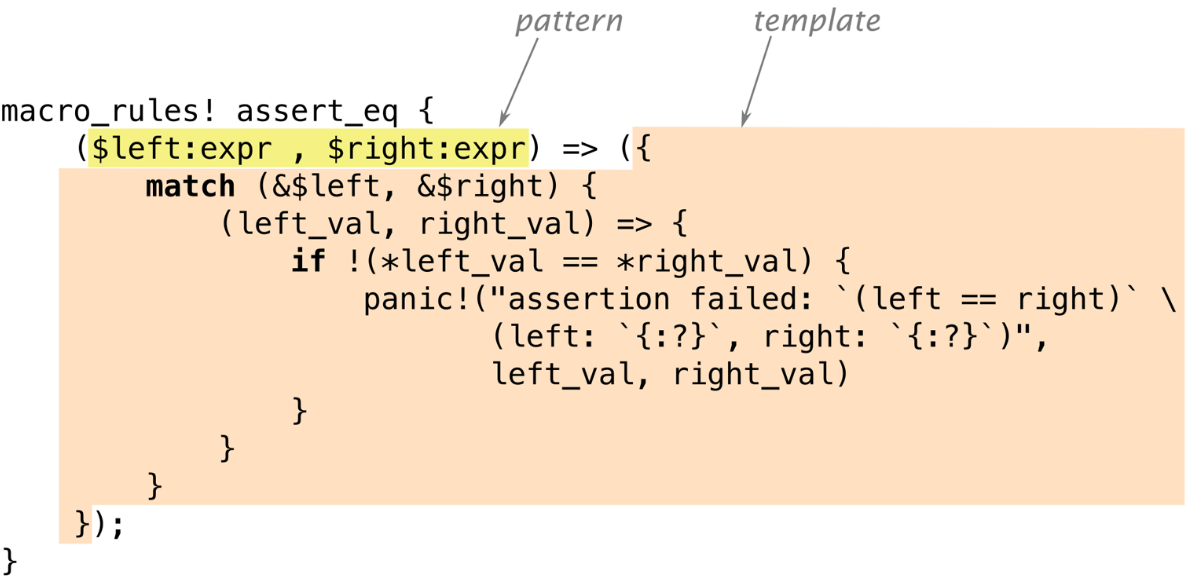
\includegraphics[width=0.9\textwidth]{../img/f21-1.png}
    \caption{\texttt{assert\_eq!}宏}
    \label{f21-1}
\end{figure}

\texttt{macro\_rules!}是Rust中定义宏的主要方法。注意,宏定义里\texttt{assert\_eq}后边没有\texttt{!}:只有在调用宏时才需要\texttt{!},定义时不需要。

并不是所有的宏都是以这种方式定义的:少数的宏,例如\texttt{file!}、\texttt{line!}和\texttt{macro\_rules!}自身,是编译器内建的。我们将在本章的末尾讨论另一种方法,称为过程宏。但我们的主要精力还是集中在\texttt{macro\_rules!},这是(目前为止)最容易的编写自己的宏的方法。

一个用\texttt{macro\_rules!}定义的宏完全靠模式匹配工作。宏的主体只是一系列规则:
\begin{minted}{text}
    ( pattern1 ) => ( template1 );
    ( pattern2 ) => ( template2 );
    ...
\end{minted}

\autoref{f21-1}中的\texttt{assert\_eq!}版本只有一个模式和一个模板。

顺便,你可以使用方括号或者花括号来代替模式或模板两侧的圆括号,对Rust来说它们并没有任何区别。另外,当你调用一个宏时,这些都是等价的:
\begin{minted}{Rust}
    assert_eq!(gcd(6, 10), 2);
    assert_eq![gcd(6, 10), 2];
    assert_eq!{gcd(6, 10), 2}
\end{minted}

唯一的不同是花括号后边的分号是可选的。为了方便,我们在调用\texttt{assert\_eq!}时使用圆括号,调用\texttt{vec!}时使用方括号,\texttt{macro\_rules!}时使用花括号。

现在我们展示了一个宏展开的简单示例和生成这个宏的定义,我们可以深入了解它工作的细节:
\begin{itemize}
    \item 我们将详细地解释Rust是怎么发现和展开你的程序中的宏定义的。
    \item 我们将指出在根据宏模板生成代码时的一些细节之处。
    \item 最后,我们将展示模式如何处理重复的结构。
\end{itemize}

\subsection{宏展开基础}
Rust会在编译的前期展开宏。编译器会从头到尾读取源码,在这个过程中定义和展开宏。宏只有在定义之后才能被调用,因为Rust会立刻展开每一个宏调用,而不会去看程序的剩余部分。(相反,函数和其他的\hyperref[static]{item}的定义不需要按照任何顺序。调用一个后面才定义的函数也是OK的。

当Rust展开一个\texttt{assert\_eq!}宏调用时,行为和执行一个\texttt{match}表达式非常像。Rust首先根据模式匹配参数,如\autoref{f21-2}所示:
\begin{figure}[htbp]
    \centering
    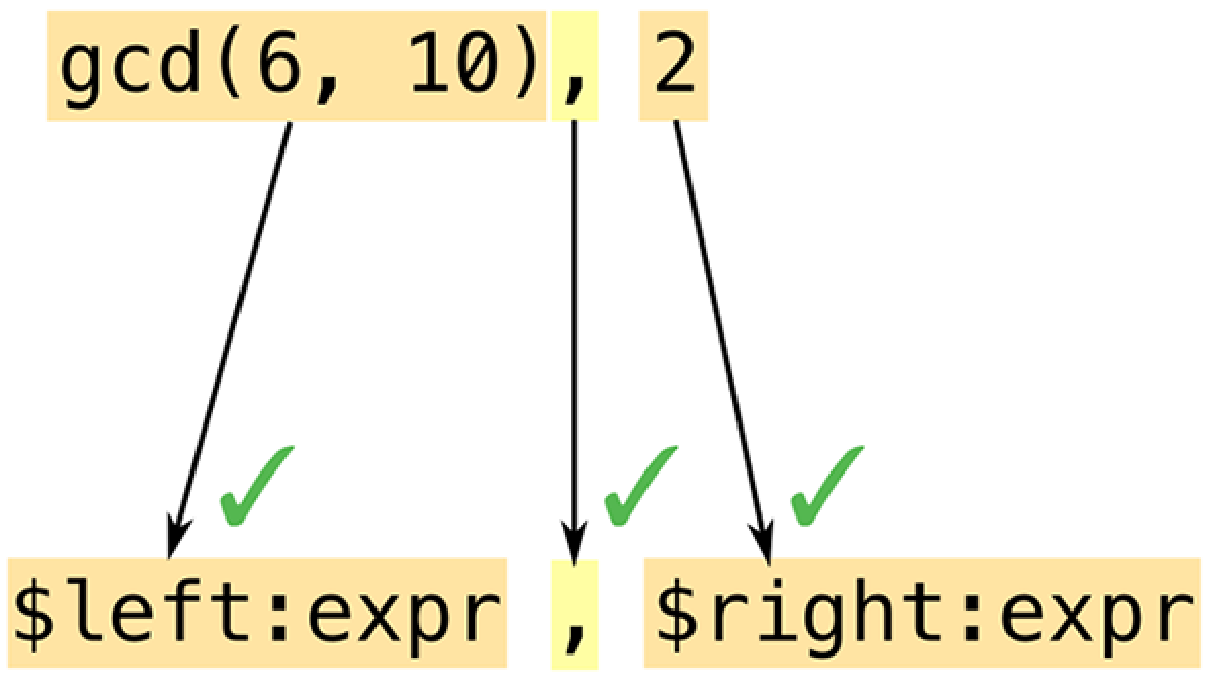
\includegraphics[width=0.8\textwidth]{../img/f21-2.png}
    \caption{展开一个宏,第1部分:用模式匹配参数}
    \label{f21-2}
\end{figure}

宏的模式是Rust的mini语言。它们本质上是匹配代码的正则表达式。但普通的正则表达式是操作字符,而模式操作\emph{token(词元)}——数字、变量名、标点符号等Rust中的构建块。这意味着你可以在宏模式中自由地使用注释和空格来提升它们的可读性。注释和空格不是token,因此它们不会影响到匹配。

正则表达式和宏模式的另一个重要不同之处是圆括号、方括号、花括号在Rust中总是成对出现。这一点会在宏展开之前就检查,不仅仅是在宏模式中,而且是在整个语言中。

在这个例子中,我们的模式包含了\emph{fragment(片段)} \texttt{\$left:expr},这告诉Rust去匹配一个表达式(在这个例子中,就是\texttt{gcd(6, 10)}并把它复制到名称\texttt{\$left}。然后Rust用\texttt{gcd}调用后边的逗号匹配模式中的逗号。类似于正则表达式,模式只有少数特殊字符会触发有趣的匹配行为;其它的所有字符,例如逗号,都必须逐字匹配相同的字符,否则就会匹配失败。

这个模式中的两个代码片段都是\texttt{expr}类型:它们代表表达式。我们将在“\nameref{FragType}”中看到其他类型的代码片段。

因为这个模式匹配到了所有的参数,Rust会展开相应的\emph{template(模板)}(\autoref{f21-3}):
\begin{figure}[htbp]
    \centering
    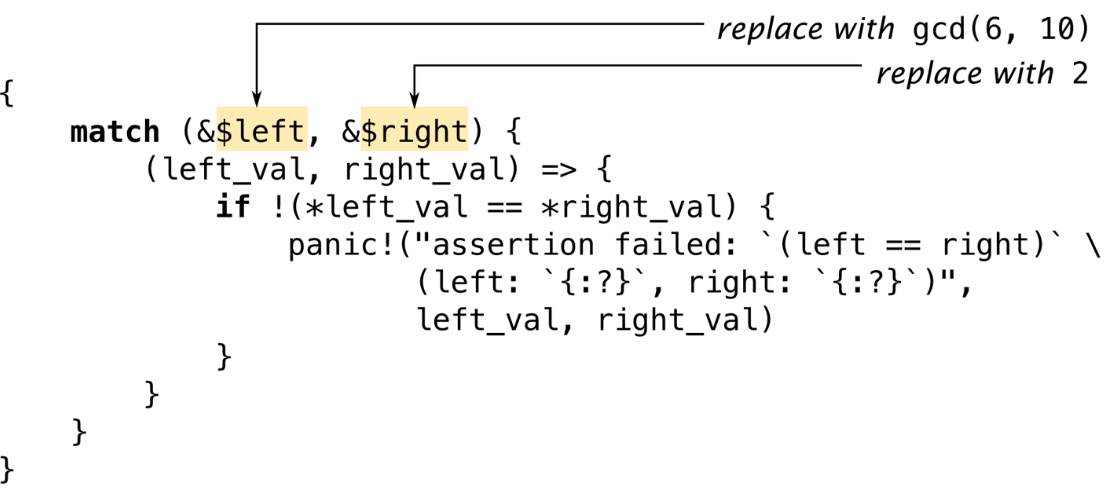
\includegraphics[width=0.9\textwidth]{../img/f21-3.png}
    \caption{展开一个宏,第2部分:填充模板}
    \label{f21-3}
\end{figure}

Rust会用匹配阶段发现的代码片段来替换\texttt{\$left}和\texttt{\$right}。

一个常见的错误是在输出模板中包含片段的类型:写\texttt{\$left:expr}而不是\texttt{\$left}。Rust不会立刻检测出这种错误。它会把\texttt{\$left}看错一个整体,然后把\texttt{:expr}看作和模板中其他部分一样的东西:要包含在宏的输出中的词元。因此只有当你\emph{调用}这个宏时这个错误才会出现;然后它会生成错误的不能编译的输出。如果你在使用一个新的宏时得到了类似\texttt{cannot find type `expr` in this scope}和\texttt{help: maybe you meant to use a path separator here}这样的错误消息,可以检查下它是不是有这个错误。(“\nameref{DebugMacro}”提供了更多类似这种情况的建议。)

宏模板和web编程中常用的很多种模板语言中的任意一种都没有太大的区别。唯一的不同——也是很重要的一点——就是它的输出是Rust代码。

\subsection{意外的结果}
把代码片段插入模板和普通的处理值的代码有一些区别。这些区别一开始可能并不明显。我们之前看到的\texttt{assert\_eq!}宏包含了一些有些奇怪的代码,这是宏编程特有的。让我们重点看看其中两个有趣的部分。

首先,为什么这个宏创建了两个变量\texttt{left\_val}和\texttt{right\_val}?为什么我们不能把模板简化成这样?
\begin{minted}{Rust}
    if !($left == $right) {
        panic!("assertion failed: `(left == right)` \
                (left: `{:?}`, right: `{:?}`)", $left, $right)
    }
\end{minted}
为了回答这个问题,尝试手动展开宏调用\texttt{assert\_eq!(letters.pop(), Some('z'))}。输出将会是什么?Rust会把匹配到的表达式插入模板中的多个位置。看起来在构建错误消息时重新求值表达式是一个坏主意,原因不仅仅是因为它需要消耗两倍的时间:因为\texttt{letters.pop()}从vector中移除一个值,所以在我们第二次调用它时会产生一个和第一次不同的值!这就是为什么真正的宏只计算一次\texttt{\$left}和\texttt{\$right},然后存储它们的值。

来到第二个问题:为什么这个宏借用了\texttt{\$left}和\texttt{\$right}的值的引用?为什么不直接把它们的\emph{值}存进变量中,像这样?
\begin{minted}{Rust}
    macro_rules! bad_assert_eq {
        ($left:expr, $right:expr) => ({
            match ($left, $right) {
                (left_val, right_val) => {
                    if !(left_val == right_val) {
                        panic!("assertion failed" /* ... */);
                    }
                }
            }
        });
    }
\end{minted}

对于我们展示过的特殊情况,即宏的参数是整数的情况下,这可以正常工作。但如果调用者传递了一个\texttt{String}变量作为\texttt{\$left}或\texttt{\$right},这段代码将会移动变量的值!
\begin{minted}{Rust}
    fn main() {
        let s = "a rose".to_string();
        bad_assert_eq!(s, "a rose");
        println!("confirmed: {} is a rose", s);    // error: use of moved value "s"
    }
\end{minted}

因为我们不想让断言移动值,所以宏里使用了引用。

(你可能想知道为什么这个宏使用了\texttt{match}而不是\texttt{let}来定义变量。我们也想知道。事实证明并没有特殊的原因这么做。\texttt{let}是等价的。)

简而言之,宏可能做出令人惊讶的行为。如果一个你写的宏附近发生了奇怪的事,那很可能是这个宏有问题。

C++里的这个经典bug你\emph{将不会}看到:
\begin{minted}{Rust}
    // buggy C++ macro to add 1 to a number
    #define ADD_ONE(n) n + 1
\end{minted}

原因大部分的C++程序员应该很熟悉了,并且不值得详细解释,类似\texttt{ADD\_ONE(1) * 10}或者\texttt{ADD\_ONE(1 << 4)}这样的代码可能会产生令人惊讶的行为。为了修复它,你需要在宏定义中加上更多括号。这在Rust中是不必要的,因为Rust宏和语言集成的更好。Rust知道它什么时候是在处理表达式,因此在把一个表达式粘贴到另一个地方时它会自动添加括号。

\subsection{重复}
标准的\texttt{vec!}宏有两种形式:
\begin{minted}{Rust}
    // 重复一个值N次
    let buffer = vec![0_u8; 1000];

    // 一个逗号分隔的值的列表
    let numbers = vec!["udon", "ramen", "soba"];
\end{minted}

它可以像这样实现:
\begin{minted}{Rust}
    macro_rules! vec {
        ($elem:expr ; $n:expr) => {
            ::std::vec::from_elem($elem, $n)
        };
        ( $( $x:expr ),* ) => {
            <[_]>::into_vec(Box::new([ $( $x ),* ]))
        };
        ( $( $x:expr ),+ ,) => {
            vec![ $( $x ),* ]
        };
    }
\end{minted}

这里有三个规则。我们将解释多个规则是如何工作的,然后依次看看每一个规则。

当Rust展开一个例如\texttt{vec![1, 2, 3]}的宏调用时,它首先尝试匹配参数\texttt{1, 2, 3}和第一条规则的模式,即\texttt{\$elem:expr ; \$n:expr}。这会匹配失败:\texttt{1}是一个表达式,但这个模式要求它后边有一个分号,然而并没有。因此Rust会移动到第二个规则,等等。如果没有规则可以匹配,就会报错。

第一个规则处理类似\texttt{vec![0u8; 1000]}这样的调用。恰好有一个标准(但不在文档里的)函数\texttt{std::vec::from\_elem},正好可以完成我们需要的功能,因此这个规则很直观。

第二个规则处理\texttt{vec!["udon", "ramen", "soba"]}。模式\texttt{\$( \$x:expr ),*}使用了一个我们之前没有提过的的特性:重复。它匹配0个或多个逗号分隔的表达式。更一般地来说,语法\texttt{\$( PATTERN ),*}用来匹配任意逗号分割的列表,其中列表中的每一项匹配\texttt{PATTERN}。

这里的\texttt{*}和正则表达式中的\texttt{*}有相同的含义(“0次或多次”),尽管正则表达式没有特殊的\texttt{,*}重复器。你也可以用\texttt{+}来要求至少一次匹配,或者用\texttt{?}要求0次或1次匹配。\autoref{t21-1}列出了全套的重复模式。

\begin{table}[htbp]
    \centering
    \caption{重复模式}
    \label{t21-1}
    \begin{tabular}{ll}
        \hline
        \textbf{模式} & \textbf{含义} \\
        \hline
        \texttt{\$( ... )*}     & 匹配0次或多次,无分隔符   \\
        \rowcolor{tablecolor}
        \texttt{\$( ... ),*}    & 匹配0次或多次,逗号分隔   \\
        \texttt{\$( ... );*}    & 匹配0次或多次,分号分隔   \\
        \rowcolor{tablecolor}
        \texttt{\$( ... )+}     & 匹配1次或多次,无分隔符   \\
        \texttt{\$( ... ),+}    & 匹配1次或多次,逗号分隔   \\
        \rowcolor{tablecolor}
        \texttt{\$( ... );+}    & 匹配1次或多次,分号分隔   \\
        \texttt{\$( ... )?}     & 匹配0次或1次,无分隔符    \\
        \rowcolor{tablecolor}
        \texttt{\$( ... ),?}    & 匹配0次或1次,逗号分隔    \\
        \texttt{\$( ... );?}    & 匹配0次或1次,分号分隔    \\
    \end{tabular}
\end{table}

代码片段\texttt{\$x}不是单个表达式,而是一个表达式的列表。这个规则的模板也使用了重复语法:
\begin{minted}{Rust}
    <[_]>::into_vec(Box::new([ $( $x ),* ]))
\end{minted}

再一次,恰好有标准方法可以满足我们的需要。这段代码创建了一个装箱的数组,然后使用\texttt{[T]::into\_vec}方法把这个装箱的数组转换成一个vector。

开头的\texttt{<[\_]>},是一种不常见的写法,它表示类型“某些东西的切片”,由Rust来推断元素类型。名字是普通标识符的类型可以直接在表达式中使用,但类似\texttt{fn()}、\texttt{\&str},或者\texttt{[\_]}这样的类型必须用尖括号包裹。

重复模式出现在模板的末尾,即\texttt{\$(\$x),*}。这个\texttt{\$(...),*}和我们在模式中看到的是相同的语法。它迭代\texttt{\$x}匹配到的表达式列表并把它们全部插入模板,用逗号分隔。

在这种情况下看,重复的输出看起来和输入一样。但并不总是这样。我们可以编写类似这样的规则:
\begin{minted}{Rust}
    ( $( $x:expr ),* ) => {
        {
            let mut v = Vec::new();
            $( v.push($x); )*
            v
        }
    };
\end{minted}

这里,模板中\texttt{\$( v.push(\$x); )*}这一部分会对\texttt{\$x}中的每个表达式插入一个\texttt{v.push()}调用。一个宏分支可以展开成一个表达式序列,但这里我们只需要单个表达式,所以我们把vector的处理包装在一个块中。

和Rust中其他部分不同,使用\texttt{\$( ... ),*}并不能自动支持可选的尾部逗号。然而,有一种标准的技巧是通过添加一个额外的规则来支持尾部逗号。也就是我们的\texttt{vec!}宏的第三条规则所做的:
\begin{minted}{Rust}
    ( $( $x:expr ),+ ,) => {    // 如果存在尾部的逗号,
        vec![ $( $x ),* ]       // 重试没有它的情况
    }
\end{minted}

我们使用\texttt{\$( ... ),+ ,}来匹配一个有额外逗号的列表。然后,我们在模板中递归调用了\texttt{vec!},但排除了那个逗号。这一次第二条规则将会匹配。

\section{内建的宏}
Rust编译器提供了几个宏,如果你要定义自己的宏,它们可能会发挥作用。这些宏都不能使用\texttt{macro\_rules!}来实现。它们被硬编码进\texttt{rustc}:

\codeentry{file!(), line!(), column!()}

\hangparagraph{\texttt{file!()}展开成一个字符串字面量:当前的文件名。\texttt{line!()}和\texttt{column!()}展开成\texttt{u32}字面量,表示当前的行号和列号(从1开始计数)。}

\hangparagraph{如果一个宏调用了另一个宏,那个宏又调用了另一个宏,这三个宏在不同的文件中,并且最后一个宏调用了\texttt{file!(), line!()}或者\texttt{column!()},它会展开成\emph{第一个}宏调用的位置。}

\codeentry{stringify!(...tokens...)}

\hangparagraph{展开成一个包含给定token的字符串字面量。\texttt{assert!}宏就是使用了它来生成一条包含了断言代码的错误信息。}

\hangparagraph{参数中的宏调用\emph{不会}被展开:\texttt{stringify!(line!())}会展开为\texttt{"line!()"}。}

\hangparagraph{Rust根据token构建字符串,因此生成的字符串里没有换行符或者注释。}

\codeentry{concat!(str0, str1, ...)}

\hangparagraph{连接参数开展为单个字符串字面量。}

Rust还定义了下面这些宏用来查询构建环境:

\codeentry{cfg!(...)}

\hangparagraph{展开为一个bool常量,如果当前的构建环境满足括号里的条件则为\texttt{true}。例如,如果在编译时启用了调试断言那么\texttt{cfg!(debug\_assertions)}为真。}

\hangparagraph{这个宏和\nameref{attribute}中介绍过的\texttt{\#[cfg(...)]}属性的语法完全相同,但它不是条件编译,而是得到一个true或者false。}

\codeentry{env!("VAR\_NAME")}

\hangparagraph{展开为一个字符串:在编译时该环境变量的值。如果这个变量不存在,会产生编译错误。}

\hangparagraph{除了Cargo在编译crate时设置的几个有趣的环境变量之外,这个宏毫无价值。例如,为了得到crate当前的版本,你可以写:}
\begin{minted}{Rust}
        let version = env!("CARGO_PKG_VERSION");
\end{minted}

\hangparagraph{这些环境变量的完整列表见\href{https://doc.rust-lang.org/cargo/reference/environment-variables.html\#environment-variables-cargo-sets-for-crates}{Cargo文档}。}

\codeentry{option\_env!("VAR\_NAME")}

\hangparagraph{它和\texttt{env!}宏一样,除了它返回一个\texttt{Option<\&'static str>},当环境变量没有设置时返回\texttt{None}。}

还有更多内建的宏可以让你引入另一个文件中的代码或者数据:
\codeentry{include!("file.rs")}

\hangparagraph{展开为指定文件的内容,必须是有效的Rust代码——表达式或者\hyperref[declaration]{item}的序列。}

\codeentry{include\_str!("file.txt")}

\hangparagraph{展开成一个包含指定文件内容的\texttt{\&'static str}。你可以像这样使用它:}

\begin{minted}{Rust}
        const COMPOSITOR_SHADER: &str =
            include_str!("../resources/compositor.glsl");
\end{minted}

\hangparagraph{如果文件不存在或者不是有效的UTF-8,会产生编译错误。}

\codeentry{include\_bytes!("file.dat")}

\hangparagraph{和上一个基本相同,除了它把文件当作二进制数据而不是UTF-8文本,结果是一个\texttt{\&'static [u8]}。}

和所有的宏一样,这些宏也是在编译时进行处理。如果文件不存在或者不能被读取,就会编译失败。它们不可能在运行时出错。在任何情况下,如果文件名是一个相对路径,它会被解析为相对于当前文件所在的目录的路径。

Rust还提供了几个方便的宏:
\codeentry{todo!(), unimplemented!()}

\hangparagraph{这些等价于\texttt{panic!()},但用于表示不同的意图。\texttt{unimplemented!()}出现在\texttt{if}分支、\texttt{march}分支,以及其它还未处理的case中。它总是会panic。\texttt{todo!()}大致相同,但传达的意图是代码还没写完;一些IDE使用它来进行标记。}

\codeentry{matches!(value, pattern)}

\hangparagraph{比较一个值和一个模式,当它们匹配时返回\texttt{true},否则返回\texttt{false}。它等价于写:}

\begin{minted}{Rust}
        match value {
            pattern => true,
            _ => false
        }
\end{minted}

\hangparagraph{如果你在寻找基本的编写宏的练习,这是一个很好的例子——尤其是你可以在标准库文档中看到它的实际实现非常简单。}

\section{调试宏}\label{DebugMacro}
调试宏可能很有挑战性。最大的问题是在宏展开的过程中缺少可视性。Rust总是展开所有宏,找到一些错误,然后打印出一条错误信息,但这个错误信息并没有显示出完整的展开后的代码!

这里有三个工具可以帮助你调试宏。(这些特性都是unstable的,但因为它们被设计为用在开发的过程中,而不是最后的代码中,因此在实践中这不是一个很大的问题。)

第一个也是最简单的一个,你可以让\texttt{rustc}显示你的代码在展开所有宏之后是什么样的。使用\texttt{cargo build --verbose}来看看Cargo是怎么调用\texttt{rustc}的。拷贝\texttt{rustc}的命令行并加上\texttt{-Z unstable-options --pretty expanded}选项。完全展开后的代码会输出到终端。不幸的是,只有当你的代码没有语法错误时这种方式才能生效。

第二,Rust提供了一个\texttt{log\_syntax!()}宏简单地在编译期把它的参数打印到终端。你可以使用它来进行\texttt{println!}风格的调试。这个宏需要\texttt{\#![feature(log\_syntax)]}特性标记。

第三,你可以让Rust编译器把所有宏调用记录到终端。在代码中插入\texttt{trace\_macros!(true)},之后每当Rust展开一个宏时,它都会打印出宏的名字和参数。例如,考虑这个程序:
\begin{minted}{Rust}
    #![feature(trace_macros)]

    fn main() {
        trace_macros!(true);
        let numbers = vec![1, 2, 3];
        trace_macros!(false);
        println!("total: {}", numbers.iter().sum::<u64>());
    }
\end{minted}

它会产生如下输出:
\begin{minted}{text}
    $ rustup override set nightly
    ...
    $ rustc trace_example.rs
    note: trace_macro
     --> trace_example.rs:5:19
      |
    5 |     let numbers = vec![1, 2, 3];
      |                   ^^^^^^^^^^^^^
      |
      = note: expanding `vec! { 1 , 2 , 3 }`
      = note: to `< [ _ ] > :: into_vec ( box [ 1 , 2 , 3 ] )`
\end{minted}
编译器会显示每一个宏调用的代码,包括展开之前和展开之后的代码。\texttt{trace\_macros!(false);}这一行关闭了追踪,因此\texttt{println!()}的调用不会被追踪。

\section{构建\texttt{json!}宏}

我们已经讨论了\texttt{macro\_rules!}的核心特性。在这一节,我们将渐进式开发一个构建JSON数据的宏。我们将用这个例子来展示开发一个宏的过程、展示\texttt{macro\_rules!}剩余的部分、并提供一些保证你的宏正确工作的建议。

回到\hyperref[ch10]{第10章},我们使用了这个枚举来代表JSON数据:
\begin{minted}{Rust}
    #[derive(Clone, PartialEq, Debug)]
    enum Json {
        Null,
        Boolean(bool),
        Number(f64),
        String(String),
        Array(Vec<Json>),
        Object(Box<HashMap<String, Json>>)
    }
\end{minted}

不幸的是,编写\texttt{Json}值的语法非常复杂:
\begin{minted}{Rust}
    let students = Json::Array(vec![
        Json::Object(Box::new(vec![
            ("name".to_string(), Json::String("Jim Blandy".to_string())),
            ("class_of".to_string(), Json::Number(1926.0)),
            ("major".to_string(), Json::String("Tibetan throat singing".to_string()))
        ].into_iter().collect())),
        Json::Object(Box::new(vec![
            ("name".to_string(), Json::String("Jason Orendorff".to_string())),
            ("class_of".to_string(), Json::Number(1702.0)),
            ("major".to_string(), Json::String("Knots".to_string()))
        ].into_iter().collect()))
    ]);
\end{minted}

我们希望能使用更类似JSON的语法来实现同样的效果:
\begin{minted}{Rust}
    let students = json!([
        {
            "name": "Jim Blandy",
            "class_of": 1926,
            "major", "Tibetan throat singing"
        },
        {
            "name": "Jason Orendorff",
            "class_of": 1702,
            "major": "Knots"
        }
    ]);
\end{minted}

我们要实现的是一个\texttt{json!}宏,它获取一个JSON值作为参数并展开为类似上一个例子中的表达式。

\subsection{片段类型}\label{FragType}
编写任何复杂宏的第一步都是指明如何匹配或\emph{解析}期望的输入。

我们已经能看到这个宏将会有好几条规则,因为JSON数据中有几种不同的东西:对象,数组,数字等等。实际上,我们可能会猜测我们将为每一种JSON类型编写一条规则:
\begin{minted}{Rust}
    macro_rules! json {
        (null)    => { Json::Null };
        ([ ... ]) => { Json::Array(...) };
        ({ ... }) => { Json::Object(...) };
        (???)     => { Json::Boolean(...) };
        (???)     => { Json::Number(...) };
        (???)     => { Json::String(...) };
    }
\end{minted}

这并不完全正确,因为宏模式没法区分最后最终三种情况,但我们稍后将会看到怎么处理它们。前三种情况至少很明显地以不同的token开头,因此我们可以用这些token进行区分。

第一个规则已经可以工作了:
\begin{minted}{Rust}
    macro_rules! json {
        (null) => {
            Json::Null
        }
    }

    #[test]
    fn json_null() {
        assert_eq!(json!(null), json::Null);    // passes!
    }
\end{minted}

为了支持JSON数组,我们可能要尝试匹配元素为\texttt{expr}:
\begin{minted}{Rust}
    macro_rules! json {
        (null) => {
            Json::Null
        };
        ([ $( $element:expr ),* ]) => {
            Json::Array(vec![ $( $element ),* ])
        };
    }
\end{minted}

不幸的是,者不能匹配所有的JSON数组。这里有一个会产生问题的例子:
\begin{minted}{Rust}
    #[test]
    fn json_array_with_json_element() {
        let macro_generated_value = json!(
            [
                // 有效的JSON,但不匹配`$element:expr`
                {
                    "pitch": 440.0
                }
            ]
        );
        let hand_coded_value =
            Json::Array(vec![
                Json::Object(Box::new(vec![
                    ("pitch".to_string(), Json::Number(440.0))
                ].into_iter().collect()))
            ]);
        assert_eq!(macro_generated_value, hand_coded_value);
    }
\end{minted}

模式\texttt{\$( \$element:expr ),*}意思是“一个逗号分隔的Rust表达式的列表”。但很多JSON值尤其是对象,不是有效的Rust表达式,它们不能匹配。

因为你想要匹配的代码并不都是表达式,所以Rust还支持其他几种片段类型,如\autoref{t21-2}所示。

\begin{table}[htbp]
    \centering
    \caption{\texttt{macro\_rules!}支持的片段类型}
    \label{t21-2}
    \begin{tabular}{lp{0.7\textwidth}p{0.2\textwidth}}
        \hline
        \textbf{片段类型}   & \textbf{匹配的内容(及示例)} &   \textbf{后边可以跟} \\
        \hline
        \texttt{expr}   & 一个表达式:\texttt{2 + 2, "udon", x.len()}   & \texttt{=> , ;}   \\
        \rowcolor{tablecolor}
        \texttt{stmt}   & 一个表达式或者声明,不包括尾部的分号(很难用;尝试用\texttt{expr}或\texttt{block}代替)   & \texttt{=> , ;} \\
        \texttt{ty} & 一个类型:\texttt{String, Vec<u8>, (\&str, bool), dyn Read + Send}    & \texttt{=> , ; | \{ [ : > as where} \\
        \rowcolor{tablecolor}
        \texttt{path}   & 一个路径(已讨论过):\texttt{ferns, ::std::sync::mpsc}   & \texttt{=> , ; | \{ [ : > as where} \\
        \texttt{pat}    & 一个模式(已讨论过):\texttt{\_, Some(ref x)}    & \texttt{=> , = | if in} \\
        \rowcolor{tablecolor}
        \texttt{item}   & 一个item(已讨论过):\texttt{struct Point \{ x: f64, y: f64 \}, mod ferns;}  & 任何东西 \\
        \texttt{block}  & 一个块(已讨论过):\texttt{\{ s += "ok\textbackslash n"; true \}}  & 任何东西  \\
        \rowcolor{tablecolor}
        \texttt{meta}   & 一个属性的内容(已讨论过):\texttt{inline, derive(Copy, Clone), doc="3D models."} & 任何东西 \\
        \texttt{ident}  & 一个标识符:\texttt{std, Json, longish\_variable\_name}   & 任何东西 \\
        \rowcolor{tablecolor}
        \texttt{literal}& 一个字面值:\texttt{1024, "Hello, world!", 1\_000\_000f64}    & 任何东西 \\
        \texttt{lifetime} & 一个生命周期:\texttt{'a, 'item, 'static}   & 任何东西 \\
        \rowcolor{tablecolor}
        \texttt{vis}    & 可见性说明符:\texttt{pub, pub(crate), pub(in module::submodule)} & 任何东西 \\
        \texttt{tt}     & 一个token树:\texttt{;, >=, \{\}, [0 1 (+ 0 1)]}  & 任何东西 \\
    \end{tabular}
\end{table}

表格中的大部分选项严格要求Rust语法。\texttt{expr}类型只匹配Rust表达式(不是JSON值),\texttt{ty}只匹配Rust类型,等等。它们是不可扩展的:没有办法定义一种新的可以用\texttt{expr}识别的运算符或关键字。我们不能用这些来实现匹配任意JSON数据。

最后两个,\texttt{ident}和\texttt{tt},支持匹配不是Rust代码的参数。\texttt{ident}匹配任何标识符。\texttt{tt}匹配单个\emph{token树}:一对正确匹配的括号:\texttt{(...), [...], \{...\}},以及其中的任何内容,包括嵌套的token树;或者一个没有括号的单个token,例如\texttt{1926}或\texttt{"Knots"}。

token树正是我们的\texttt{json!}宏所需要的。每一个JSON值都是单个token树:数字、字符串、bool值、\texttt{null}都是单个token,对象和数组是token树。因此我们可以写出像这样的模式:
\begin{minted}{Rust}
    macro_rules! json {
        (null) => {
            Json::Null
        };
        ([ $( $element:tt ),* ]) => {
            Json::Array(...)
        };
        ({ $( $key:tt : $value: tt),* }) => {
            Json::Object(...)
        };
        ($other::tt) => {
            ... // TODO: 返回数字、字符串、bool值
        };
    }
\end{minted}

这个版本的\texttt{json!}宏可以匹配任何JSON数据。现在我们只需要产生正确的Rust代码。

为了保证Rust在未来可以添加新的语法特性而不会破坏任何你今天写的宏,Rust限制了模式中紧跟在片段之后的token。\autoref{t21-2}中“后边可以跟”这一列展示了哪些token可以跟在模式后面。例如,模式\texttt{\$x:expr ~ \$y:expr}是错的,因为\texttt{~}不允许出现在\texttt{expr}后面。模式\texttt{\$vars:pat => \$handler:expr}是可以的,因为\texttt{\$vars:pat}后跟的是箭头\texttt{=>},它允许跟在\texttt{pat}后面,而\texttt{\$handler:expr}后面没有跟任何东西,这种情况总是允许的。

\subsection{宏中的递归}
我们已经见过了一个在宏里调用自身的小例子:我们的\texttt{vec!}的实现使用了递归来支持尾部的逗号。这里我们可以展示一个更加显著的例子:\texttt{json!}需要递归调用它自身。

我们可能会尝试在不递归的情况下支持JSON数组,像这样:
\begin{minted}{Rust}
    ([ $( $element:tt ),* ]) => {
        Json::Array(vec![ $( $element ),* ])
    };
\end{minted}
但这段代码并不能工作。这样只是把JSON数据(\texttt{\$element} token树)粘贴到了Rust表达式之中,但它们是两种不同的语言。

我们需要把数组中的每一个元素从JSON格式转换为Rust代码。幸运的是,有一个宏可以做到这件事:就是我们正在写的这个宏!
\begin{minted}{Rust}
    ([ $( $element:tt ),* ]) => {
        Json::Array(vec![ $( json!($element) ),* ])
    };
\end{minted}

这种方式还可以支持对象:
\begin{minted}{Rust}
    ({ $( $key:tt : $value:tt ),* }) => {
        Json::Object(Box::new(vec![
            $( ($key.to_string(), json!($value)) ),*
        ].into_iter().collect()))
    };
\end{minted}

默认情况下编译器会把宏的递归次数上限设置为64。对于\texttt{json!}宏的常规使用这肯定已经足够了,但有时复杂的递归宏会达到这个上限。你可以在使用这个宏的crate的开头加上这一行来调整上限
\begin{minted}{Rust}
    #![recursion_limit = "256"]
\end{minted}
我们的\texttt{json!}宏基本已经完成了。剩下的只有支持布尔、数字和字符串值。

\subsection{宏和trait}
编写复杂的宏时总是会遇到困难。重要的是要记住,宏并不是解决问题的唯一途径。

这里,我们需要支持\texttt{json!(true)}、\texttt{json!(1.0)}、\texttt{json!("yes")},把这些值转换成对应的\texttt{Json}值。但宏并不擅长区分类型。假如我们这么写:
\begin{minted}{Rust}
    macro_rules! json {
        (true) => {
            Json::Boolean(true)
        };
        (false) => {
            Json::Boolean(false)
        };
        ...
    }
\end{minted}

显然这种方案是行不通的。布尔类型只有两个值,但数字和字符串有很多值。

幸运的是,有一种标准的把多种类型的值转换成另一种特定类型的方法:\texttt{From} trait。我们可以简单地为几种类型实现这个trait:
\begin{minted}{Rust}
    impl From<bool> for Json {
        fn from(b: bool) -> Json {
            Json::Boolean(b)
        }
    }

    impl From<i32> for Json {
        fn from(i: i32) -> Json {
            Json::Number(i as f64)
        }
    }

    impl From<String> for Json {
        fn from(s: String) -> Json {
            Json::String(s)
        }
    }

    impl<'a> From<&'a str> for Json {
        fn from(s: &'a str) -> Json {
            Json::String(s.to_string())
        }
    }
    ...
\end{minted}

事实上,所有的12种数字类型应该有非常相似的实现,因此编写一个宏来避免复制粘贴是有意义的:
\begin{minted}{Rust}
    macro_rules! impl_from_num_for_json {
        ( $( $t:ident )* ) => {
            $(
                impl From<$t> for Json {
                    fn from(n: $t) -> Json {
                        Json::Number(n as f64)
                    }
                }
            )*
        };
    }

    impl_from_num_for_json!(u8 i8 u16 i16 u32 i32 u64 i64 u128 i128
                            usize isize f32 f64);
\end{minted}

现在我们可以使用\texttt{Json::from(value)}来把\texttt{value}转换成\texttt{Json}。在我们的宏中,看起来像这样:
\begin{minted}{Rust}
    ( $other:tt ) => {
        Json::from($other)  // 处理布尔/数字/字符串
    };
\end{minted}

向我们的\texttt{json!}宏中添加了这个规则之后,它就可以通过我们目前写过的所有测试了。把所有部分汇总起来,它现在看起来像这样:
\begin{minted}{Rust}
    macro_rules! json {
        (null) => {
            Json::Null
        };
        ([ $( $element:tt),* ]) => {
            Json::Array(vec![ $( json!($element) ),* ])
        };
        ({ $( $key:tt : $value:tt ),* }) => {
            Json::Object(Box::new(vec![
                $( ($key.to_string(), json!($value)) ),*
            ].into_iter().collect()))
        };
        ( $other:tt ) => {
            Json::from($other)  // 处理布尔/数字/字符串
        };
    }
\end{minted}

事实证明,这个宏意外地支持在JSON数据中使用变量甚至任意的Rust表达式,这是一个有趣的特性:
\begin{minted}{Rust}
    let width = 4.0;
    let desc = 
        json!({
            "width": width,
            "height": (width * 9.0 / 4.0)
        });
\end{minted}

因为\texttt{(width * 9.0 / 4.0)}是用括号括起来的,所以它是单个的token树,因此在解析这个对象时宏可以成功地用\texttt{\$value:tt}匹配它。

\subsection{作用域和hygiene}
在编写宏时一个令人惊讶的问题是它们将来自不同范围的代码粘贴在一起。因此接下来的几页将介绍Rust处理作用域的两种方式:一种用于局部变量和参数,另一种用于其他的东西。

为了展示为什么会有这个问题,让我们重写解析JSON对象的规则(之前展示过的\texttt{json!}宏的第三条规则),让它不再使用临时的vector。我们可以像这样写:
\begin{minted}{Rust}
    ({ $($key:tt : $value:tt),* }) => {
        {
            let mut fields = Box::new(HashMap::new());
            $( fields.insert($key.to_string(), json!($value)); )*
            Json::Object(fields)
        }
    };
\end{minted}

现在我们不再使用\texttt{collect()},而是通过重复调用\texttt{.insert()}方法来填充\texttt{HashMap}。这意味着我们需要把map存储在一个临时的变量中,这里命名为\texttt{fields}。

但如果调用\texttt{json!}宏的代码中恰好也有一个叫\texttt{fields}的变量,会发生什么呢?
\begin{minted}{Rust}
    let fields = "Fields, W.C.";
    let role = json!({
        "name": "Larson E. Whipsnade",
        "actor": fields
    });
\end{minted}

展开这个宏时将会把两段代码拼在一起,两段代码中都用了变量\texttt{fields}来表示不同的东西!
\begin{minted}{Rust}
    let fields = "Fields, W.C.";
    let role = {
        let mut fields = Box::new(HashMap::new());
        fields.insert("name".to_string(), Json::from("Larson E. Whipsnade"));
        fields.insert("actor".to_string(), Json::from(fields));
        Json::Object(fields)
    };
\end{minted}

看起来好像只要宏里使用了临时变量就无法避免这个问题,并且你可能已经正在思考可能的解决方案了。也许我们应该把\texttt{json!}宏中的变量重命名为一般情况下调用者不会传入的名字:例如用\texttt{\_\_json\$fields}代替\texttt{fields}。

这里令人惊讶的是\emph{宏可以正常工作}。Rust会为你重命名变量!这个特性一开始在Scheme宏中实现,被称为\emph{hygiene},因此Rust被认为有\emph{hygienic宏}。

理解hygiene宏的最简单的方式就是想象每一次展开宏时,展开的部分都被染成了不同的颜色。

不同颜色的变量,就好像有不同的名字一样:
\begin{figure*}[h]
    \centering
    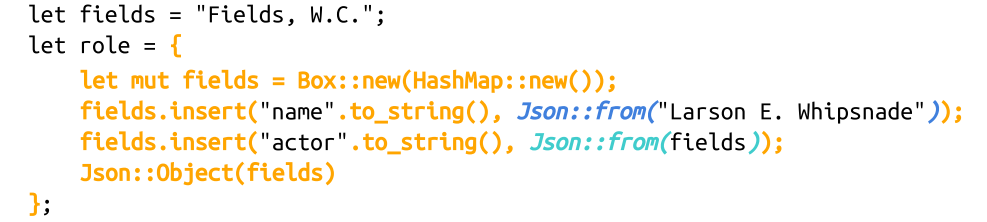
\includegraphics[width=0.8\textwidth]{../img/f21-4.png}
\end{figure*}

注意这里宏的调用者传入并被粘贴到输出中的代码,例如\texttt{"name"}和\texttt{"actor"},保持了它们原本的颜色(黑色)。只有宏模板生成的token被染成了另一种颜色。

现在这里有一个叫\texttt{fields}的变量(在调用者中声明)和另一个叫\texttt{fields}的变量(宏引入的)。因为这两个名字的颜色不同,所以这两个变量不会混淆。

如果一个宏真的需要引用一个在调用者作用于里的变量,那么调用者必须向宏传递这个变量的名字。

(染色的比喻并不意味着hygiene真的就是这么工作的。实际的机制要更聪明一些:不管是什么颜色,如果两个标识符引用了宏和调用者作用域里的同一个变量,那么就认为它们是相同的。但在Rust中像这样的例子非常少见。如果你理解了上面的例子,那么就使用hygiene宏来说已经足够了。)

你可能已经注意到了很多别的标识符也被染上了一种或多种的颜色:例如\texttt{Box}、\texttt{HashMap}、\texttt{Json}等。就算没有颜色,Rust也可以辨认出这些类型的名字。这是因为Rust中的hygiene仅限于局部变量和参数。对于常量、类型、昂发、模块、静态变量、宏名来说,Rust是“色盲”。

这意味着如果我们的\texttt{json!}宏被用在了\texttt{Box}、\texttt{HashMap}或\texttt{Json}不在作用域里的模块中时,这个宏将不能工作。我们将在下一节中展示怎么避免这个问题。

首先,我们将考虑一个Rust的hygiene会产生阻碍的例子,并且我们需要解决它。假设我们有很多函数都包含下面这一行代码:
\begin{minted}{Rust}
    let req = ServerRequest::new(server_socket.session());
\end{minted}

如果复制粘贴这一行将会很痛苦。我们可以使用宏来代替吗?
\begin{minted}{Rust}
    macro_rules! setup_req {
        () => {
            let req = ServerRequest::new(server_socket.session());
        }
    }

    fn handle_http_request(server_socket: &ServerSocket) {
        setup_req!();   // 声明`req`,使用了`server_socket`
        ... // 使用`req`的代码
    }
\end{minted}

显然这么写不能工作。必须要让宏里的\texttt{server\_socket}这个名字指向函数里声明的参数\texttt{server\_socket},\texttt{req}变量恰好相反。但hygiene会保护宏里的名字不会和其他作用域里的名字“碰撞”——即使这正是你想要的行为。

解决方案是把你计划在宏里宏外都要使用的变量全部传进宏里:
\begin{minted}{Rust}
    macro_rules! setup_req {
        ($req:ident, $server_socket:ident) => {
            let $req = ServerRequest::new($server_socket.session());
        }
    }

    fn handle_http_request(server_socket: &ServerSocket) {
        setup_req!(req, server_socket);
        ... // 使用`req`的代码
    }
\end{minted}

因为\texttt{req}和\texttt{server\_socket}现在由函数提供,所以它们的“颜色”和那个作用域一样。

hygiene让宏的使用变得更繁琐了一点,但这是一个特性,而不是bug:知道了它们不会在背后扰乱局部变量之后,可以更容易地推理hygiene宏。如果你在一个函数里搜索一个类似\texttt{server\_socket}的标识符,你将会发现所有使用了它的地方,包括宏调用。

\subsection{导入和导出宏}

    \chapter{unsafe代码}\label{ch22}

\emph{Let no one think of me that I am humble or weak or passive; \\
Let them understand I am of a different kind: dangerous to my enemies, loyal to my friends. \\
To such a life glory belongs.}

系统级编程的乐趣在于,在每一个安全的语言和精心设计的抽象之下,都是不安全的机器语言和比特位。你也可以在Rust中写出这样的代码。

到目前为止本书中介绍的语言部分,例如类型、生命周期、约束检查等都可以自动保证你的程序完全没有内存错误和数据竞争。但这种自动的技术有它的局限性;Rust并不能识别出来很多有价值的技术是安全的。

\emph{unsafe代码}让你可以告诉Rust,“我要使用一些你不能保证安全的特性”。把一个块或者函数标记为unsafe之后,你就可以调用标准库中的\texttt{unsafe}函数、解引用unsafe指针、调用其他语言例如C和C++编写的函数等。Rust的其他安全性检查依然生效:类型检查、生命周期检查、约束检查等仍然和之前一样。unsafe代码只是允许了一小部分额外的特性。

正是因为有了允许超出safe Rust界限的能力,Rust才能实现它自身的大部分基础特性,和C/C++一样,Rust也被用来实现它自己的标准库。unsafe代码可以让\texttt{Vec}类型更高效地管理它的缓冲区;让\texttt{std::io}模块和操作系统交互;让\texttt{std::thread}和\texttt{std::sync}模块提供并发原语。

本章介绍了unsafe特性的一些基础:

\begin{enumerate}
    \item Rust的\texttt{unsafe}块区分开了普通的safe Rust代码和使用unsafe特性的代码。
    \item 你可以把函数标记为\texttt{unsafe},提醒调用者他们必须遵守的一些额外约束来避免未定义行为。
    \item 原始指针和它们的方法运行对内存进行不受限的访问,并允许你构建Rust的类型系统可能禁止的数据结构。Rust的引用虽然安全,但却是受限制的,原始指针正如每个C或C++程序员所知,是一个强大而锋利的工具。
    \item 理解未定义行为的定义将会帮助你理解为什么它们比得到错误结果还要糟糕的多。
    \item unsafe trait,类似于\texttt{unsafe}函数,隐含了每个实现(而不是每个调用者)都要遵守的规则。
\end{enumerate}

\section{unsafe从何而来?}
在本书的开头处,我们曾经展示过一个C程序,它以一种非常令人惊讶的方式崩溃。这是因为它违背了C标准的一个规则。你可以在Rust中实现相同的效果:

\begin{minted}{bash}
    $cat crash.rs
    fn main() {
        let mut a: usize = 0;
        let ptr = &mut a as *mut usize;
        unsafe {
            *ptr.offset(3) = 0x7ffff72f484c;
        }
    }
    $ cargo build
       Compiling unsafe-samples v0.1.0
        Finished debug [unoptimized + debuginfo] target(s) in 0.44s
    $ ../../target/debug/crash
    crash: Error: .netrc file is readable by others.
    crash: Remove password or make file unreadable by others.
    Segmentation fault (core dumped)
    $
\end{minted}

这个程序借用了局部变量\texttt{a}的一个可变引用,然后把它转换成了\texttt{*mut usize}类型的原始指针,然后使用了它的\texttt{offset}方法来产生一个指向三个字之后的位置的指针。这里恰巧存储了\texttt{main}的返回地址。这个程序用一个常量覆盖了返回地址,因此从\texttt{main}返回之后程序的行为就很奇怪。这个崩溃之所以可行,是因为程序错误使用了unsafe的特性——在这个例子中,就是解引用原始指针的能力。

一个unsafe特性通常隐含了一份\emph{合约(contract)}:即一组Rust不能自动强制,但你必须遵守才能避免\emph{未定义行为}的规则。

一份合约超出了普通的类型检查和生命周期检查,它们隐含着一些unsafe特性特定的规则。通常来说,Rust本身完全不知道这些合约,它们只在unsafe特性的文档里得到解释。例如,原始指针类型的合约是禁止解引用一个指向的位置超出原来指向物的末尾的原始指针。这个例子中的表达式\texttt{*ptr.offset(3) = ...}打破了这个合约。但是,正如上面所示,Rust没有任何警告,成功编译了这个程序:它的安全检查并没有检测出来这个违规行为。当你使用unsafe特性时,你作为程序员,需要负责检查你的代码遵守了它们的合约。

很多特性如果想正确使用,都要遵守一定的规则。但这些规则并不是我们这里说的合约,除非它们可能会导致未定义行为。未定义行为是一种Rust假设你的代码中绝对不会出现的行为。例如,Rust假设你不会用别的值覆盖函数的返回地址。通过了Rust通常的安全检查并且遵守了使用到的unsafe特性的合约的代码不可能会出现这样的行为。因为这个程序违反了原始指针的合约,因此它的行为变得未定义,并最终崩溃。

如果你的代码出现了未定义行为,说明你打破了你负责的一部分,Rust拒绝预测结果。从系统库的深处抛出来一个错误并崩溃是一种可能的结果;把你的计算机的控制权交给攻击者是另一种可能的结果。不同的Rust版本可能也会有不同的行为。然而,有时未定义行为不一定会产生可见的结果。例如,如果这里的\texttt{main}函数永远不会返回(可能调用了\texttt{std::process::exit})来提前终止程序),那么错误的返回地址也无关紧要。

你只能在\texttt{unsafe}块或者\texttt{unsafe}函数里使用unsafe特性;我们将在接下来的小节介绍它们。它们让unsafe特性不容易被忽略:通过强迫你写一个\texttt{unsafe}块或者函数,Rust能确保你知道你的代码可能要遵守一些额外的规则。

\section{unsafe块}
\texttt{unsafe}块看起来就像一个以\texttt{unsafe}关键字开头的普通块,区别在于你可以在unsafe块里使用unsafe特性:
\begin{minted}{Rust}
    unsafe {
        String::from_utf8_unchecked(ascii)
    }
\end{minted}

如果没有块前面的\texttt{unsafe}关键字,Rust将会禁止使用\texttt{from\_utf8\_unchecked},因为它是一个\texttt{unsafe}的函数。在\texttt{unsafe}块中,你可以随意使用它。

和普通的Rust块一样,\texttt{unsafe}块的值也是最后一条表达式的值,或者是\texttt{()}。这个例子中\texttt{String::from\_utf8\_unchecked}的调用提供了块的值。

一个\texttt{unsafe}块为你解锁了5个额外的功能:
\begin{enumerate}
    \item 你可以调用\texttt{unsafe}函数。每一个\texttt{unsafe}函数都有它自己的合约,这取决于它的功能。
    \item 你可以解引用原始指针。safe代码可以传递、比较、通过引用转换创建原始指针,但只有unsafe代码才可以使用它们来访问内存。我们将在\nameref{rawp}中详细介绍原始指针并解释如何安全地使用它们。
    \item 你可以访问\texttt{union}的字段,尽管编译器不能确定它们含有相应类型的有效值。
    \item 你可以访问可变的\texttt{static}变量。正如\nameref{globalvar}中解释的一样,Rust不能确保什么时候有线程正在使用可变的\texttt{static}变量,因此它们的合约要求你要确保所有的访问都是正确同步的。
    \item 你可以访问通过Rust的外部函数接口声明的函数和变量。即使它们是不可变的,也会被认为是\texttt{unsafe}的,因为它们是使用其他语言编写的,这些语言可能不遵守Rust的安全规则。
\end{enumerate}

把unsafe特性约束在\texttt{unsafe}块里并不会真的阻止你做任何想做的事。你完全只需要在你的代码里加上一个\texttt{unsafe}块,然后就可以继续了。这个规则的作用主要是为了把人类的注意力吸引到那些Rust不能保证安全性的代码上:
\begin{enumerate}
    \item 你不会意外地使用到unsafe特性,然后发现你要为甚至不知道它的存在的合约负责。
    \item 一个\texttt{unsafe}块可以吸引reviewer更多的注意力。一些项目甚至有一些自动化流程来确保这一点,例如标记出会影响\texttt{unsafe}块的代码来吸引更多注意力。
    \item 当你正在考虑编写一个\texttt{unsafe}块时,你可以花费一点时间来问问自己你的任务是否真的需要这些特性。如果是为了性能,你是否有测量数据表明这真的是一个性能瓶颈?可能有一种在safe Rust中也可以实现相同效果的方法。
\end{enumerate}

\section{示例:一个高效的ASCII字符类型}
这里有一个示例,\texttt{Ascii}是一个字符串类型,它确保它的内容总是有效的ASCII字符。这个类型使用一个unsafe特性来提供到\texttt{String}的0开销转换:
\begin{minted}{Rust}
    mod my_ascii {
        /// 一个ASCII编码的字符串
        #[derive(Debug, Eq, PartialEq)]
        pub struct Ascii(
            // 它必须只存有有效的ASCII文本:从`0`到`0x7f`的字节序列
            Vec<u8>
        );

        impl Ascii {
            /// 从`bytes`中的Ascii文本创建一个`Ascii`。
            /// 如果`bytes`中含有任何非ASCII字符就返回一个`NotAsciiError`错误。
            pub fn from_bytes(bytes: Vec<u8>) -> Result<Ascii, NotAsciiError> {
                if bytes.iter().any(|&byte| !byte.is_ascii()) {
                    return Err(NotAsciiError(bytes));
                }
                Ok(Ascii(bytes))
            }
        }

        // 当转换失败时,我们会给出不能转换的vector。
        // 它应该实现`std::error::Error`,这里为了简洁就省略了。
        #[derive(Debug, Eq, PartialEq)]
        pub struct NotAsciiError(pub Vec<u8>);

        // 安全、高效的转换,使用unsafe代码实现。
        impl From<Ascii> for String {
            fn from(ascii: Ascii) -> String {
                // 如果这个模块没有bug的话,这里就是安全的,
                // 因为有效的ASCII文本也是有效的UTF-8文本。
                unsafe { String::from_utf8_unchecked(ascii.0) }
            }
        }
        ...
    }
\end{minted}

这个模块的关键是\texttt{Ascii}类型的定义。这个类型本身被标记为\texttt{pub},来让它在\texttt{my\_ascii}模块外可见。但它的\texttt{Vec<u8>}元素\emph{不是}public的,因此只有\texttt{my\_ascii}模块里的方法可以创建一个\texttt{Ascii}值或者访问它的元素。这完全控制了模块里哪些代码是公开的哪些是不公开的。只要public的构造器和方法能确保新创建的\texttt{Ascii}值是有效的,并始终保持有效,那么程序的其他部分就不可能违反规则。并且public的构造器\texttt{Ascii::from\_bytes}确实小心地检查了给定的vector来确保能从它构建出一个有效的\texttt{Ascii}。出于简洁性的考虑,我们并没有展示出每一个方法,但你可以想象还有一些处理文本的方法,这些方法同样确保\texttt{Ascii}的值总是有效的ASCII文本,就像\texttt{String}的方法确保它的内容总是有效的UTF-8.

这样的安排让我们可以非常高效地为\texttt{String}实现\texttt{From<Ascii>}。unsafe函数\texttt{String::from\_utf8\_unchecked}获取一个字节vector并根据它的内容构建一个\texttt{String},并且不检查它的内容是否是有效的UTF-8文本;这个函数的合约就是调用者要负责这一点。幸运的是,\texttt{Ascii}类型强迫的规则正是满足\texttt{from\_utf8\_unchecked}的合约所需的条件。正如我们在\nameref{utf8}中解释的一样,任何有效的ASCII文本都是有效的UTF-8文本,因此\texttt{Ascii}内部的\texttt{Vec<u8>}可以立刻作为一个\texttt{String}的缓冲区使用。

有了这些定义之后,你可以写这样的代码:
\begin{minted}{Rust}
    use my_ascii::Ascii;

    let bytes: Vec<u8> = b"ASCII and ye shall receive".to_vec();

    // 这里的调用没有任何内存分配或者文本拷贝,只进行一次扫描。
    let ascii: Ascii = Ascii::from_bytes(bytes)
        .unwrap();  // 我们已经知道了bytes是没问题的。

    // 这里的调用是0开销的:没有内存分配、拷贝、扫描。
    let string = String::from(ascii);

    assert_eq!(string, "ASCII and ye shall receive");
\end{minted}

使用\texttt{Ascii}不需要unsafe块。我们已经使用unsafe操作实现了一个safe的接口,并且安排好只依赖模块自己的代码而不是用户的行为来满足它的合约。

\texttt{Ascii}只是一个\texttt{Vec<u8>}的包装,并在模块里隐藏了一些强迫它的内容需要满足的规则。一个这样的类型被称为\emph{newtype},它是Rust中非常普遍的一种模式。Rust自己的\texttt{String}类型就使用完全相同的方式定义的,区别只有它的内容被限制为UTF-8,而不是ASCII。事实上,这是标准库里\texttt{String}的定义:
\begin{minted}{Rust}
    pub struct String {
        vec: Vec<u8>,
    }
\end{minted}

在机器语言的层面上,是完全没有Rust的类型信息的,一个newtype和它的元素有完全相同的内存表示,因此构建一个newtype完全不需要任何额外的机器指令。在\texttt{Ascii::from\_bytes}中,表达式\texttt{Ascii(bytes)}只是表明\texttt{Vec<u8>}现在的内存表示持有的是一个\texttt{Ascii}值。类似的,\texttt{String::from\_utf8\_unchecked}在内联的情况下可能不包含任何机器指令:它只表明\texttt{Vec<u8>}现在被认为是一个\texttt{String}。

\section{unsafe函数}
\texttt{unsafe}函数的定义就像一个以\texttt{unsafe}开头的普通函数。\texttt{unsafe}函数的函数体自动被认为是一个\texttt{unsafe}块。

你只能在\texttt{unsafe}块里调用\texttt{unsafe}函数。这意味着将一个函数标记为\texttt{unsafe}可以警告调用者这个函数有一个额外的合约,必须满足这个合约才能避免未定义行为。

例如,这里有一个新的\texttt{Ascii}类的构造器,这个构造器从一个字节vector构建一个\texttt{Ascii},并且不检查内容是否是有效的ASCII:
\begin{minted}{Rust}
    // 这段代码必须放在`my_ascii`模块中。
    impl Ascii {
        /// 从`bytes`构建一个`Ascii`值,不检查`bytes`是否是有效的ASCII文本。
        ///
        /// 这个函数直接返回一个`Ascii`,而不是像`from_bytes`一样返回一个
        /// `Result<Ascii, NotAsciiError>`。
        ///
        /// # 安全性
        ///
        /// 调用者必须确保`bytes`只包含ASCII字符:每个字节都不大于0x7f。
        /// 否则,最后的结果是未定义的。
        pub unsafe fn from_bytes_unchecked(bytes: Vec<u8>) -> Ascii {
            Ascii(bytes)
        }
    }
\end{minted}

如果调用\texttt{Ascii::from\_bytes\_unchecked}的代码总是知道vector中只包含有效的ASCII字符,那么\texttt{Ascii::from\_bytes}里的检查就只是在浪费时间,并且调用者还必须处理永远不会出现的\texttt{Err}结果。\texttt{Ascii::from\_bytes}可以简化这种情况下的调用和错误处理。

但之前我们曾经强调过\texttt{Ascii}的public构造器和方法保证\texttt{Ascii}的值是有效的的重要性。\texttt{from\_bytes\_unchecked}是不是没有遵守这个规则?

不完全是:\texttt{from\_bytes\_unchecked}把它的责任通过它的合约交给了调用者。这个合约的存在正是它应该被标记为\texttt{unsafe}的原因:虽然这个函数本身没有进行unsafe的操作,但它的调用者必须遵守一些Rust不能强制的规则才能避免未定义行为。

你真的能通过打破\texttt{Ascii::from\_bytes\_unchecked}的合约来导致未定义行为吗?是的。你可以像下面这样构造一个无效的\texttt{String}:
\begin{minted}{Rust}
    // 想象这个vector是一些我们认为会产生ASCII文本的操作的结果,
    // 但这个操作出错了。
    let bytes = vec![0xf7, 0xbf, 0xbf, 0xbf];
    let ascii = unsafe {
        // 当`bytes`含有非ASCII值时这个unsafe的合约就被打破了
        Ascii::from_bytes_unchecked(bytes)
    };

    let bogus: String = ascii.into();

    // `bogus` 现在包含无效的UTF-8。
    // 解析它的第一个字符会产生一个无效的Unicode码点的`char`,
    // 这是未定义行为,因此Rust不知道这个断言的行为会是什么样的。
    assert_eq!(bogus.chars().next().unwrap() as u32, 0x1fffff);
\end{minted}

在特定版本的Rust和特定的平台上,这个断言会输出下面的错误信息并失败:
\begin{minted}{text}
    thread 'main' panicked at 'assertion failed: `(left == right)`
      left: `2097151`
     right: `2097151`, src/main.rs:42:5
\end{minted}

这两个数字在我们看来似乎是相等的,但这不是Rust的问题;这是之前的\texttt{unsafe}块的问题。当我们说未定义行为会导致无法预料的结果时,这就是其中一种情况。

这个例子展示了两个有关bug和unsafe代码的关键事实:
\begin{enumerate}
    \item \emph{\texttt{unsafe}块之前发生的bug可能会打破合约}。一个\texttt{unsafe}块是否会导致未定义行为可能不仅仅取决于这个块本身,还取决于提供它要操作的值的代码。你的\texttt{unsafe}代码依赖的任何东西都是和安全相关的。只有当模块的其他部分正确的维护了\texttt{Ascii}相关的内容时,基于\texttt{String::from\_utf\_unchecked}的\texttt{Ascii}到\texttt{String}的转换才是安全的。
    \item \emph{打破合约的结果可能在你离开\texttt{unsafe}块之后才会出现}。不遵守unsafe特性而导致的未定义行为通常不会在\texttt{unsafe}块本身里出现。如上面所示,构造一个bogus \texttt{String}可能不会有问题,直到程序的程序执行中才出现问题。
\end{enumerate}

本质上讲,Rsut的类型检查、借用检查和其他的静态检查都是在分析你的程序并尝试证明它不可能会出现未定义行为。当Rust成功编译你的程序时,这意味着它成功地证明了这一点。一个\texttt{unsafe}块是这个证明中的例外:等于你在告诉Rust“它没有问题,相信我”。你的声明是否正确可能依赖程序的任何会影响到\texttt{unsafe}块的部分,并且出错时产生的结果也可能出现在任何被\texttt{unsafe}块影响的地方。\texttt{unsafe}关键字也是在提醒你,你无法完全享受到它的安全检查的好处。

如果可以选择的话,你应该尽量选择使用安全的没有合约的接口。它们更容易使用,因为用户可以依赖Rust的安全检查来保证他们的代码不可能出现未定义行为。即使你的实现使用了unsafe特性,最好使用Rust的类型、生命周期和模块系统来满足它们的合约,同事只使用你自己就可以保证的,而不是把责任传递给调用者。

不幸的是,在实际编程中遇到懒得解释它们的合约的unsafe函数并不罕见。他们期望你能依靠自己的经验和知识自己推导出这些规则。

\section{unsafe块还是unsafe函数?}
你可能会想知道是使用\texttt{unsafe}块还是直接把整个函数标记为unsafe。我们推荐的方法是首先判断函数:
\begin{enumerate}
    \item 如果这个函数可能被误用,可以成功编译但可能导致未定义行为,那么你应该将它标记为unsafe。正确使用这个函数的规则就是它的合约,也正是合约的存在让它变得unsafe。
    \item 否则,这个函数是safe的:没有调用能让它产生未定义行为。它不应该被标记为\texttt{unsafe}。
\end{enumerate}

这个函数在函数体里是否使用unsafe特性并不这个重要,关键是合约的存在。之前我们展示过一个没有使用unsafe特性的unsafe函数,也展示过一个使用了unsafe特性的safe函数。

不要只因为你在函数体里使用了unsafe特性就把safe的函数标记为\texttt{unsafe}。这只会让函数更难用,并且迷惑调用者,让他以为这里有一个合约。正确的做法是使用一个\texttt{unsafe}块,即使这个块就是整个函数体。

\section{未定义行为}
在引言中,我们说过术语\emph{未定义行为}意思是“Rust假设你的代码绝对不会出现的行为”。这是一个奇怪的说法,尤其是我们通过其他语言积累的经验告诉我们这些行为\emph{确实}会偶然出现。为什么这个概念有助于规定unsafe代码的义务?

编译器是从一种编程语言到另一种语言的转换器。Rust编译器接收一个Rust程序并把它翻译成等价的机器语言程序。但两个差别大的语言,我们说它们等价到底是什么意思?

幸运的是,相比于语言学家,对程序员来说这个问题简单的多。如果两个程序执行时总是有相同的可见的行为,那么我们说这两个程序是等价的:它们进行相同的系统调用、以等价的方式和外部函数交互等等。这有点像程序的图灵测试:如果你不能分辨出你是在和原始的程序交互还是和翻译后的程序交互,那么它们就是等价的。

现在考虑下面的代码:
\begin{minted}{Rust}
    let i = 10;
    very_trustworthy(&i);
    println!("{}", i * 100);
\end{minted}

即使我们完全不知道\texttt{very\_trustworthy}的定义,我们可以看到它只接收一个\texttt{i}的共享引用,因此这个调用不可能改变\texttt{i}的值。因此传递给\texttt{println!}的值将总是\texttt{1000},Rust可以把这段代码翻译成机器语言,就好像我们写的是:
\begin{minted}{Rust}
    very_trustworthy(&10);
    println!("{}", 1000);
\end{minted}

这个转换后的版本和原本的有相同的可见的行为,而且它可能还要更快一点。但只有在我们认同它真的和原始的版本相同的时候考虑它的性能才有意义。如果\texttt{very\_trustworthy}被定义成这样呢?
\begin{minted}{Rust}
    fn very_trustworthy(shared: &i32) {
        unsafe {
            // 把这个共享引用转换成一个可变的指针。
            // 这是未定义行为。
            let mutable = shared as *const i32 as *mut i32;
            *mutable = 20;
        }
    }
\end{minted}

这段代码打破了共享引用的规则:它把\texttt{i}的值改成了\texttt{20},但\texttt{i}是以共享的方式借用的。因此,现在对这个函数的调用者进行转换会产生非常明显的效果:如果Rust转换了这段代码,程序会打印出\texttt{1000};如果它保留了这段代码并使用\texttt{i}的新值,它会打印出\texttt{2000}。在\texttt{very\_trustworthy}中打破共享引用的规则意味着共享引用的行为并不会如调用者所预期。

这类问题出现在几乎每种Rust会尝试进行的转换中。包括把一个函数内联到调用者中、当调用结束后控制流返回到调用处,等等。但是我们以一个打破了这种假设的的例子来开始这一章。

对Rust(或其他任何语言)来说基本不可能判断对程序的转换是否能保持它的含义,除非它可以信任语言的基础特性的行为和预期一样。它们是否会进行这种转换不仅依赖于眼下的代码,还可能依赖潜在的很远之外的代码。为了对你的代码做一点改动,Rust必须假设程序的其他部分的行为都是正常的。

然后这里是Rust对行为正确程序的规则:
\begin{enumerate}
    \item 程序绝对不能读取未初始化的内存。
    \item 程序绝对不能创建无效的基础值:
    \begin{enumerate}
        \item 引用、box或函数指针为\texttt{null}
        \item 既不是\texttt{0}也不是\texttt{1}的\texttt{bool}值
        \item 判断值无效的\texttt{enum}
        \item 无效的\texttt{char}值,非Unicode码点
        \item 内容不是有效的UTF-8的\texttt{str}值
        \item 虚表或者切片长度无效的胖指针
        \item \texttt{!}类型的任何值
    \end{enumerate}
    \item \autoref{ch05}中介绍的引用的规则必须要遵守。不能有引用的生命周期比引用的对象更长;共享的访问是只读访问,可变的访问是独占的访问。
    \item 程序绝对不能解引用空的、错误对齐的、或悬垂的指针。
    \item 程序绝对不能用一个指针去访问超出这个指针关联的对象的内存范围之外的位置。我们将在\nameref{DerefRawP}中详细解释这个规则。
    \item 程序必须没有数据竞争。数据竞争发生在两个线程在未同步的情况下访问相同的内存位置,并且其中至少有一个访问是写入访问。
    \item 程序绝对不能在一个其他语言通过外部函数接口所进行的调用中进行栈展开,正如在\nameref{unwind}中解释的一样。
    \item 程序必须遵守标准库函数的合约。
\end{enumerate}

由于我们还没有Rust的\texttt{unsafe}语义的完整模型,这个列表可能会随着时间的推移而改变,但这些内容很可能仍然是禁止的。

任何违反这些规则的行为都可能构成未定义行为,还会阻止Rust优化你的程序并把它们转换成机器语言。如果你打破了最后一个规则把无效的UTF-8传递给\texttt{String::from\_utf8\_unchecked},那么之后可能2097151不等于2097151。

不使用unsafe特性的Rust代码只要能编译就能被保证遵守上述所有规则(假设编译器没有bug,我们正在逐渐靠近这个目标,但曲线和渐近线永远不会相交)。只有当你使用unsafe特性时,这些规则才会变成你自己的责任。

在C和C++中,即使你的程序没有报错成功通过了编译也意义不大;正如我们在这本书的引言中解释的,即使是用那些保持高标准代码的广受欢迎的库编写的最好的C和C++程序在实践中也会出现未定义行为。

\section{unsafe trait}\label{UnsafeTrait}
\emph{\texttt{unsafe} trait}是一种特殊的trait,它们有一个Rust无法检查或者强制实现必须遵守的规则,实现必须遵守这些规则才能避免未定义行为。为了实现一个unsafe trait,你必须将实现标记为unsafe的。理解trait的合约并确保你的实现满足合约是你的责任。

一个用unsafe trait来约束类型变量的函数通常自身也会使用unsafe特性,并且它们只依赖这些unsafe trait的合约来满足自己的合约。一个错误的trait实现可能会导致这样的函数出现未定义行为。

\texttt{std::marker::Send}和\texttt{std::marker::Sync}是unsafe trait的典型例子。这些trait并没有定义任何方法,因此可以很容易地为任何类型实现它们。但它们确实有合约:\texttt{Send}要求实现者可以安全地移动到另一个线程中,\texttt{Sync}要求实现者必须能安全地通过共享引用在线程间共享。为一个不恰当的类型实现\texttt{Send}将会使\texttt{std::sync::Mutex}不能再保证没有数据竞争。

这里有个简单的例子,Rust标准库曾经包含了一个叫\texttt{core::nonzero::Zeroable}的unsafe trait,它用来表示那些可以通过把所有字节置为0来安全地初始化的类型。举个例子,把一个\texttt{usize}置0是可以的,但把一个\texttt{\&T}置0会产生空引用,如果解引用就会崩溃。对于那些实现了\texttt{Zeroable}的类型,有一些可行的优化:你可以使用\texttt{std::ptr::write\_bytes}(\texttt{memset}在Rust中的等价函数)或者一个分配置0内存页的系统调用来快速地初始化它们的数组。(\texttt{Zeroable}是unstable的,并且在Rust 1.26中被移到只在\texttt{num} crate中内部使用,但它是一个好的、简单的、真实的例子。)

\texttt{Zeroable}是一个类型标记trait,没有方法或者关联类型:
\begin{minted}{Rust}
    pub unsafe trait Zeroable {}
\end{minted}

为恰当的类型实现这个trait非常的直观:
\begin{minted}{Rust}
    unsafe impl Zeroable for u8 {}
    unsafe impl Zeroable for i32 {}
    unsafe impl Zeroable for usize {}
    // 其他的整数类型同理
\end{minted}

有了这些定义,我们可以编写一个函数,它可以快速地分配一个给定长度的\texttt{Zeroable}类型的vector:
\begin{minted}{Rust}
    use core::nonzero::Zeroable;

    fn zeroed_vector<T>(len: usize) -> Vec<T>
        where T: Zeroable
    {
        let mut vec = Vec::with_capacity(len);
        unsafe {
            std::ptr::write_bytes(vec.as_mut_ptr(), 0, len);
            vec.set_len(len);
        }
        vec
    }
\end{minted}

这个函数首先用给定的容量创建一个空的\texttt{Vec},然后调用\texttt{write\_bytes}用0来填充未初始化的缓冲区。(\texttt{write\_bytes}函数把\texttt{len}看做\texttt{T}类型元素的数量,而不是字节的数量,因此这个调用确实填充了整个缓冲区。)vector的\texttt{set\_len}方法只修改它的长度,不对缓冲区进行任何操作;这是unsafe的,因为你必须保证新的缓冲区空间内都包含正确初始化的\texttt{T}类型的值。但这正是\texttt{T: Zeroable}约束的:一个0字节的块代表一个有效的\texttt{T}值。我们对\texttt{set\_len}的使用是安全的。

这里,我们来使用它:
\begin{minted}{Rust}
    let v: Vec<usize> = zeroed_vector(100_000);
    assert!(v.iter().all(|&u| u == 0));
\end{minted}

显然\texttt{Zeroable}必须是一个unsafe的trait,因为一个不遵守合约的实现可能导致未定义行为:
\begin{minted}{Rust}
    struct HoldsRef<'a>(&'a mut i32);

    unsafe impl<'a> Zeroable for HoldsRef<'a> { }

    let mut v: Vec<HoldsRef> = zeroed_vector(1);
    *v[0].0 = 1;    // 崩溃:解引用空指针
\end{minted}

Rust不知道\texttt{Zeroable}表示什么,所以它不能分辨出哪些类型的实现是不恰当的。和其他的unsafe特性一样,理解并遵守unsafe trait的合约是你的责任。

注意unsafe代码绝对不能依赖正确实现的普通的safe trait。例如,假设有一个\texttt{std::hash::Hasher} trait的实现简单地返回一个随机的哈希值,这个值和被哈希的值没有一点关系。这个trait要求同样的值两次被哈希时必须产生相同的哈希值,但这个现实并不满足这个要求;它很显然是错误的。但因为\texttt{Hasher}并不是unsafe的trait,unsafe代码在使用这个哈稀器的时候不应该出现未定义行为。\texttt{std::collections::HashMap}类型是被精心编写的,它遵守所有用到的unsafe特性的合约,不管哈稀器的行为是什么样的。具体的来说,即使哈希表不能正确地工作:查找可能失败,表项可能随机出现或者消,整个表也不会出现未定义行为。

\section{原始指针}\label{rawp}
Rust中\emph{原始指针}指的是没有约束的指针。你可以使用原始指针来组织Rust的普通指针类型无法做到的数据结构,例如双向链表或者任意的图对象。但因为原始指针太过灵活,Rust无法分辨出你是否正在安全地使用它们,因此你只能在\texttt{unsafe}块中解引用它们。

原始指针基本等价于C或C++中的指针,因此在和这些语言编写的代码交互时原始指针非常有用。

有两种原始指针:
\begin{enumerate}
    \item \texttt{*mut T}是可以修改引用对象的指针。
    \item \texttt{*const T}是只能读取引用对象的指针。
\end{enumerate}
(没有\texttt{*T}类型,你必须指定\texttt{const}或者\texttt{mut}。)

你可以通过转换引用来创建原始指针,并使用\texttt{*}操作符来解引用它:
\begin{minted}{Rust}
    let mut x = 10;
    let ptr_x = &mut x as *mut i32;

    let y = Box::new(20);
    let ptr_y = &*y as *const i32;

    unsafe {
        *ptr_x += *ptr_y;
    }
    assert_eq!(x, 30);
\end{minted}

和box指针以及引用不同,原始指针可以为null,类似C中的\texttt{NULL}和C++中的\texttt{nullptr}:
\begin{minted}{Rust}
    fn option_to_raw<T>(opt: Option<&T>) -> *const T {
        match opt {
            None => std::ptr::null(),
            Some(r) => r as *const T
        }
    }

    assert!(!option_to_raw(Some(&("pea", "pod"))).is_null());
    assert_eq!(option_to_raw::<i32>(None), std::ptr::null());
\end{minted}

这个例子中没有\texttt{unsafe}块:创建、传递、比较原始指针都是safe的。只有解引用原始指针才是unsafe的。

unsized类型的原始指针是胖指针,就像相应的引用或\texttt{Box}指针一样。一个\texttt{*const [u8]}的指针除了地址之外还包括长度,一个trait对象的原始指针例如\texttt{*mut dyn std::io::Write}指针还附带一个虚表。

尽管Rust在很多场景可以隐式解引用safe的指针类型,但原始指针的解引用必须是显式的:
\begin{enumerate}
    \item \texttt{.}运算符不会隐式解引用原始指针,你必须用\texttt{(*raw).field}或者\texttt{(*raw).method(...)}。
    \item 原始指针并没有实现\texttt{Deref},因此强制解引用并不适用于它们。
    \item \texttt{==}和\texttt{<}之类的运算符以地址比较原始指针:只有两个原始指针指向同一个内存位置它们才是相等的。类似,哈希一个原始指针会对它指向的地址进行哈希,而不是对它指向的对象的值进行哈希。
    \item 格式化trait例如\texttt{std::fmt::Dispaly}会自动解引用,但无法处理原始指针。例外的是\texttt{std::fmt::Debug}和\texttt{std::fmt::Pointer},它们会以16进制地址的形式显示原始指针,不会解引用它们。
\end{enumerate}

和C/C++中的\texttt{+}运算符不同,Rust的\texttt{+}运算符不能用于原始指针,但你可以使用原始指针的\texttt{offset}、\texttt{wrapping\_offset}或者更方便的\texttt{add}、\texttt{sub}、\texttt{wrapping\_add}、\texttt{wrapping\_sub}方法对它们进行算数操作。\texttt{offset\_from}方法可以给出两个指针之间的距离,不过我们必须确保起点和终点在相同的内存区域(例如在同一个\texttt{Vec})里:
\begin{minted}{Rust}
    let trucks = vec!["grabage truck", "dump truck", "moonstruck"];
    let first: *const &str = &trucks[0];
    let last: *const &str = &trucks[2];
    assert_eq!(unsafe { last.offset_from(first) }, 2);
    assert_eq!(unsafe { first.offset_from(last) }, -2);
\end{minted}

\texttt{first}和\texttt{last}不需要隐式转换,只要指明类型就够了。Rust隐式地把引用强制转换为原始指针(当然反过来不行)。

\texttt{as}运算符允许几乎把任何引用转换成原始指针或者转换两个原始指针类型。然而,你必须把一个复杂的转换拆分成一系列简单的转换。例如:
\begin{minted}{Rust}
    &vec![42_u8] as *const String;  // 错误:无效转换
    &vec![42_u8] as *const Vec<u8> as *const String;    // 允许
\end{minted}

注意\texttt{as}不能把原始指针转换为引用。这样的转换是unsafe的,而\texttt{as}应该保证是safe的操作。要想做到这一点,你必须解引用原始指针(在一个\texttt{unsafe}块中)然后借用得到的值的引用。

这么做的时候一定要小心:这种方式产生的引用将会有无限的生命周期:它的生存时间没有任何限制,因为原始指针并没有给Rust提供推断这一点的信息。在后面的\nameref{SafeInter}一节中,我们将展示几个例子来演示如何正确地约束生命周期。

很多类型都有\texttt{as\_ptr}和\texttt{as\_mut\_ptr}方法可以返回它们的内容的原始指针。例如,数组的切片和字符串会返回它们的第一个元素的指针,一些迭代器会返回它们要产生的下一个元素的指针。拥有所有权的指针类型例如\texttt{Box}、\texttt{Rc}和\texttt{Arc}有\texttt{into\_raw}和\texttt{from\_raw}函数可以转换成或转换自原始指针。其中一些方法的合约有一些令人惊讶的要求,因此在使用之前要仔细阅读它们的文档。

你也可以把整数转换成原始指针,尽管你唯一可以信任的整数是从之前的指针得到整数。\nameref{RefWithFlag}以这种方式使用了原始指针。

和引用不同,原始指针既没有实现\texttt{Send}也没有实现\texttt{Sync}。因此,任何包含原始指针的类型默认都没有实现这两个trait。在线程间发送或者共享原始指针本质上并没有什么不安全的,毕竟,不管它们去了哪,在解引用它们的时候仍然需要一个\texttt{unsafe}块。但考虑到原始指针通常扮演的角色,语言的设计者认为默认是这样会更有帮助。我们已经在\nameref{UnsafeTrait}中讨论过如何自己实现\texttt{Send}和\texttt{Sync}了。

\subsection{安全地解引用原始指针}\label{DerefRawP}
这里有一些安全使用原始指针的基本规则:
\begin{enumerate}
    \item 解引用空指针或悬垂指针是未定义行为,指向未初始化内存或超出作用域的值的指针也是如此。
    \item 解引用没有按照类型正确对齐的指针是未定义行为。
    \item 你可以从解引用原始指针获得的值借用引用,不过只有当这么做满足\autoref{ch05}中介绍的引用安全性规则时才可以:引用不能超出被引用对象的生命周期、共享的访问是只读的访问、可变的访问是独占的访问。(这个规则很容易在无意中被违反,因为原始指针通常被用来创建非标准共享或所有权的数据结构。)
    \item 只有当一个原始指针指向的对象是正确的该类型的值时你才能使用它指向的对象。例如,你必须确保解引用一个\texttt{*const char}返回一个正确的Unicode码点。
    \item 在使用原始指针的\texttt{offset}和\texttt{wrapping\_offset}方法时你必须确保最后指向的位置还在一开始指向的那个对象的值或者内存块里。\\ 如果你先把一个指针转换成整数,然后进行任何的算术运算,再把它转换回指针,那么结果必须是\texttt{offset}的规则允许你产生的指针。
    \item 如果你对原始指针指向的对象赋值,你必须保证不违反其中任何一个类型的不变量。例如,如果你有一个指向一个\texttt{String}的字节的\texttt{*mut u8}指针,你对这个\texttt{u8}赋的值必须保证\texttt{String}持有的仍是有效的UTF-8。
\end{enumerate}

除了借用规则之外,这些都是在C和C++中使用指针时必须要遵守的基本规则。

不能违背类型的不变量的原因应该很清楚。很多Rust的标准类型在实现里都使用了unsafe代码,但仍然提供了safe的接口。它们假设Rust的安全检查、模块系统和可见性规则都没有被违反。使用原始指针来绕开这些保护措施可能会导致未定义行为。

完整又精确的原始指针的合约很难简单地说清楚,也可能会随着语言的改进发生改变。但这里列出的原则应该能保证代码是安全的。

\subsection{示例:\texttt{RefWithFlag}}\label{RefWithFlag}
这里有一个例子展示了怎么使用原始指针来进行一些经典的位级操作并把它包装为一个完全安全的Rust类型。这个模块定义了一个类型\texttt{RefWithFlag<'a, T>},它持有一个\texttt{\&'a T}和一个\texttt{bool},类似于元组\texttt{(\&'a, bool)}一样。但它只占用一个机器字而不是两个。这种技术通常用在垃圾回收器和虚拟机中,其中的某些类型(例如表示任意对象的类型)的实例非常多,以至于如果能减小一个机器字就可以大大减少内存占用:
\begin{minted}{Rust}
    mod ref_with_flag {
        use std::marker::PhantomData;
        use std::mem::align_of;

        ///
        pub struct RefWithFlag<'a, T> {
            ptr_and_bit: usize,
            behaves_like: PhantomData<&'a T> // 不占用空间
        }

        impl<'a, T: 'a> RefWithFlag<'a, T> {
            pub fn new(ptr: &'a T, flag: bool) -> RefWithFlag<T> {
                assert!(align_of::<T>() % 2 == 0);
                RefWithFlag {
                    ptr_and_bit: ptr as *const T as usize | flag as usize,
                    behaves_like: PhantomData
                }
            }

            pub fn get_ref(&self) -> &'a T {
                unsafe {
                    let ptr = (self.ptr_and_bit & !1) as *const T;
                    &*ptr
                }
            }

            pub fn get_flag(&self) -> bool {
                self.ptr_and_bit & 1 != 0
            }
        }
    }
\end{minted}

这段代码利用了很多类型必须放在偶数的内存地址处:因为一个偶数地址的最低有效位总是0,因此我们可以在这里存储一些东西,然后只要把它置0就能还原原来的地址。并不是所有类型都能这么做;例如,类型\texttt{u8}和\texttt{(bool, [i8; 2])}可以被放在任何地址处。但我们可以在初始化时检查类型的对齐然后拒绝不适用的类型。

我们可以像这样使用\texttt{RefWithFlag}:
\begin{minted}{Rust}
    use ref_with_flag::RefWithFlag;

    let vec = vec![10, 20, 30];
    let flagged = RefWithFlag::new(&vec, true);
    assert_eq!(flagged.get_ref()[1], 20);
    assert_eq!(flagged.get_flag(), true);
\end{minted}

\texttt{RefWithFlag::new}接收一个引用和一个\texttt{bool}值,之后断言引用的类型是合适的,然后把引用转换为一个原始指针,再转换成\texttt{usize}。不管我们在什么处理器上编译,\texttt{usize}类型都足够存储任何指针,因此把一个原始指针转换成\texttt{usize}再转换回来是良定义的。一旦我们有了一个\texttt{usize},我们知道它肯定是偶数,因此我们可以使用\texttt{|}位或运算符把它和\texttt{bool}值结合在一起,当然要先把\texttt{bool}值转换成0或者1。

\texttt{get\_flag}方法从一个\texttt{RefWithFlag}中提取出\texttt{bool}的部分。这很简单,只要看看最低位是否非零。

\texttt{get\_ref}方法从一个\texttt{RefWithFlag}中提取出引用部分。首先,它把\texttt{usize}的最低位置0后转换为原始指针。\texttt{as}运算符不能把原始指针转换成引用,但我们可以解引用原始指针(当然是在\texttt{unsafe}块中)然后借用引用。借用原始指针指向对象的引用会产生一个没有生命周期约束的引用:如果可行的话,Rust会给任何引用赋予一个生命周期,用于检查代码。然而,通常有一些生命周期会更加准确,因此也能检查出更多的错误。在这种情况下,因为\texttt{get\_ref}的返回类型是\texttt{\&'a T},Rust会看到引用的生命周期和\texttt{RefWithFlag}的生命周期参数\texttt{'a}相同,这正是我们想要的:这正是一开始的那个引用的生命周期。

在内存中,一个\texttt{RefWithFlag}看起来就像一个\texttt{usize}:因为\texttt{PhantomData}是一个0字节类型,\texttt{behaves\_like}字段不会占用任何空间。但为了让Rust知道如何处理使用了\texttt{RefWithFlag}的代码的生命周期,\texttt{PhantomData}是必须的。想象一下如果没有\texttt{behaves\_like}字段,这个类型的定义会变成什么样:
\begin{minted}{Rust}
    // 不能通过编译。
    pub struct RefWithFlag<'a, T: 'a> {
        ptr_and_bit: usize
    }
\end{minted}

在\autoref{ch05}中,我们指出过任何包含引用的结构体必须不能比它们借用的值生存的更久,否则引用会变成悬垂指针。结构体必须在它的字段上遵守这个限制。这当然也适用于\texttt{RefWithFlag}:在我们刚才看过的示例代码中,\texttt{flagged}必须不能比\texttt{vec}生存的更久,因为\texttt{flagged.get\_ref()}返回一个它的引用。但我们的缩减版的\texttt{RefWithFlag}类型根本不包含任何引用,甚至都没用到生命周期参数\texttt{'a},它只是一个\texttt{usize}。Rust应该如何知道该对\texttt{flagged}的生命周期进行什么限制?包含一个\texttt{PhantomData<\&'a T>}字段可以告诉Rust处理\texttt{RefWithFlag<'a, T>}时,\emph{就好像}它还含有一个\texttt{\&'a T}一样,这并不会影响结构体在内存中的表示。

尽管Rust并不真的知道发生了什么,它也会尽力帮你实现这些。如果你省略了\texttt{behaves\_like}字段,Rust将会报错说生命周期\texttt{'a}和\texttt{T}都没有用到,然后建议使用\texttt{PhantomData}。

\texttt{RefWithFlag}和我们之前展示过的\texttt{Ascii}类型使用了相同的策略来避免未定义行为。这个类型本身是\texttt{pub}的,但它的字段不是,这意味着只有在\texttt{ref\_with\_flag}模块内的代码可以创建或访问\texttt{RefWithFlag}值。你不需要检查太多代码就能确信\texttt{ptr\_and\_bit}字段始终是正确构造的。

\subsection{可空的指针}
Rust中的空原始指针和C/C++中一样,都是0地址。对任何类型\texttt{T},\texttt{std::ptr::null<T>}函数会返回一个\texttt{*const T}空指针,\texttt{std::ptr::null\_mut<T>}返回一个\texttt{*mut T}空指针。

有一些方法可以检查一个原始指针是不是空的。最简单的是\texttt{is\_null}方法,但\texttt{as\_ref}方法可能会更加便捷:它接受一个\texttt{*const T}指针然后返回一个\texttt{Option<\&'a T>},把空指针转换为\texttt{None}。类似的,\texttt{as\_mut}方法把一个\texttt{*mut T}转换成\texttt{Option<\&'a mut T>}。

\subsection{类型大小和对齐}
一个\texttt{Sized}类型的值在内存中的字节数是固定的,并且必须放置在一个是\emph{对齐}值倍数的地址处。例如,一个\texttt{(i32, i32)}元组占用8个字节,几乎所有的处理器都喜欢把它放在一个4的倍数的地址处。

\texttt{std::mem::size\_of::<T>()}返回\texttt{T}类型的字节数,\texttt{std::mem::align\_of::<T>()}返回它要求的对齐数。例如:
\begin{minted}{Rust}
    assert_eq!(std::mem::size_of::<i64>(), 8);
    assert_eq!(std::mem::align_of::<(i32, i32)>(), 4);
\end{minted}

任何类型的对齐总是2的幂。

一个类型的大小通常向上取它的对齐的倍数,即使从技术上讲它用不了那么多空间。例如,虽然元组\texttt{(f32, u8)}只需要5个字节,但\texttt{size\_of::<(f32, u8)>()}是8,因为\texttt{align\_of<(f32, u8)>()}是4。这确保了如果有一个数组,那么元素大小的大小总是等于一个元素到下一个元素的距离。

对于unsized的类型,大小和对齐取决于具体的值。给第一个unsized值的引用,\texttt{std::mem::size\_of\_val}和\texttt{std::mem::align\_of\_val}函数返回这个值的大小和对齐。这些函数可以同时用于\texttt{Sized}和unsized类型:
\begin{minted}{Rust}
    // 切片的胖指针会携带长度。
    let slice: &[i32] = &[1, 3, 9, 27, 81];
    assert_eq!(std::mem::size_of_val(slice), 20);

    let text: &str = "alligator";
    assert_eq!(std::mem::size_of_val(text), 9);

    use std::fmt::Display;
    let unremarkable: &dyn Dispaly = &193_u8;
    let remarkable: &dyn Dispaly = &0.0072973525664;

    // 这些函数返回trait对象指向的值的大小和对齐,
    // 而不是trait对象本身。
    // 这些信息来自于trait对象引用的虚表。
    assert_eq!(std::mem::size_of_val(unremarkable), 1);
    assert_eq!(std::mem::align_of_val(remarkable), 8);
\end{minted}

\subsection{指针算术}

Rust把数组、切片或者vector布局为单个连续的内存块,如\autoref{f22-1}所示。元素都被按规律放置,这样如果每个元素占用\texttt{size}个字节,那么第\texttt{i}个元素从\texttt{i * size}处开始。

\begin{figure}[htbp]
    \centering
    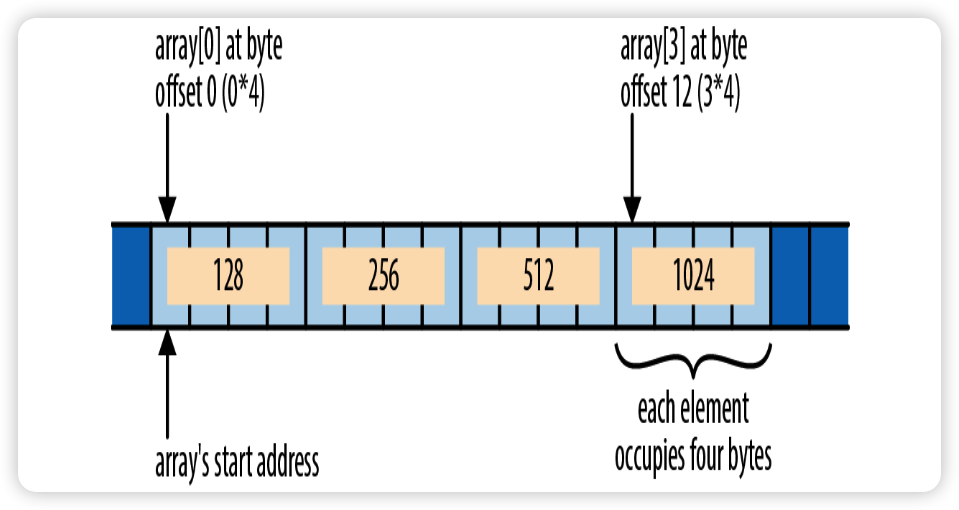
\includegraphics[width=0.9\textwidth]{../img/f22-1.png}
    \caption{内存中的数组}
    \label{f22-1}
\end{figure}

这样做的一个好处如果你有两个指向同一个数组中元素的原始指针,比较这两个指针和比较两个元素的索引的结果是一样的:如果\texttt{i < j},那么指向第\texttt{i}个元素的原始指针小于指向第\texttt{j}个元素的原始指针。这让原始指针作为数组遍历的边界时很有用。事实上,标准库中最简单的迭代切片的迭代器就是这样定义的:
\begin{minted}{Rust}
    struct Iter<'a, T> {
        ptr: *const T,
        end: *const T,
        ...
    }
\end{minted}

\texttt{ptr}字段指向下一个要产生的元素,\texttt{end}字段作为边界:当\texttt{ptr == end}时,说明迭代结束了。

数组布局的另一个好处是:如果\texttt{element\_ptr}是一个指向第\texttt{i}个元素的\texttt{*const T}或\texttt{*mut T}原始指针,那么\texttt{element\_ptr.offset(o)}就是指向第\texttt{i + o}个元素的原始指针。它的定义等价于这样:
\begin{minted}{Rust}
    fn offset<T>(ptr: *const T, count: isize) -> *const T
        where T: Sized
    {
        let bytes_per_element = std::mem::size_of::<T>() as isize;
        let byte_offset = count * bytes_per_element;
        (ptr as isize).checked_add(byte_offset).unwrap() as *const T
    }
\end{minted}

\texttt{std::mem::size\_of::<T>}函数返回\texttt{T}类型的字节数。因为\texttt{isize}足够存储一个地址,因此可以把指针转换为\texttt{isize},然后对这个值进行算术运算,最后把结果转换为指针。

创建一个指向数组尾部之后第一个字节的指针是可以的。你不能解引用这样的指针,但它可以用于表示循环的结束或者边界检查。

然而,使用\texttt{offset}创建一个指向数组尾部之后或者头部之前的指针是未定义行为,即使你甚至没有解引用它。为了优化,Rust会假设当\texttt{i}是正数时\texttt{ptr.offset(i) > ptr},当\texttt{i}是负数时\texttt{ptr.offset(i) < ptr}。这个假设看起来是安全的,但如果\texttt{offset}中的算术运算溢出了\texttt{isize}值的范围它可能是不成立的。如果\texttt{i}被约束为保证最后的结果仍然和\texttt{ptr}指向同一个数组,那就不可能会溢出:数组自身不可能溢出地址空间的边界。(为了保证指向尾部后第一个字节的指针是安全的,Rust绝不会把值放置在地址空间的最顶端。)

如果你的确需要把指针偏移到超出指向的数组,你可以使用安全的\texttt{wrapping\_offset}方法。它等价于\texttt{offset},但Rust对\texttt{ptr.wrapping\_offset(i)}和\texttt{ptr}的相对大小不做任何假设。当然,除非最后的结果还落在数组里,不然你仍然不能解引用它。

\subsection{移进和移出内存}
如果你在实现一个管理它自己的内存的类型,你将需要追踪内存里哪些部分存储了还在生命周期内的值,以及哪些部分是未初始化的,就像Rust处理局部变量一样。考虑这段代码:
\begin{minted}{Rust}
    let pot = "pasta".to_string();
    let plate = pot;
\end{minted}

当这段代码运行之后,内存布局看起来如\autoref{f22-2}所示。

\begin{figure}[htbp]
    \centering
    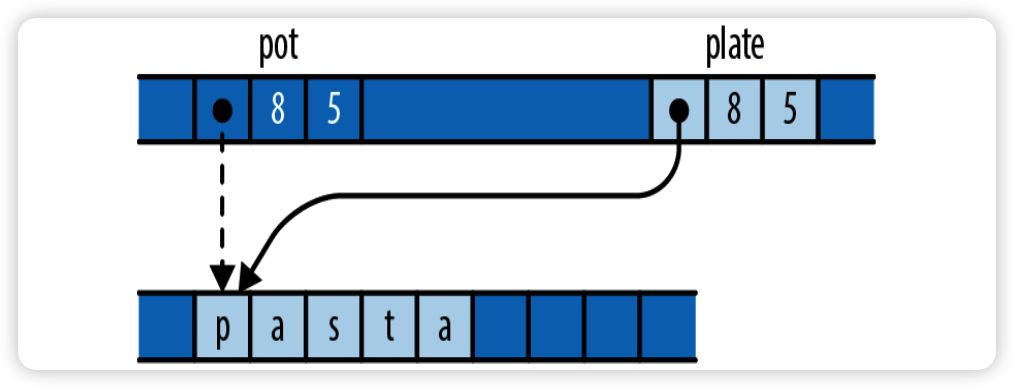
\includegraphics[width=0.9\textwidth]{../img/f22-2.png}
    \caption{把一个字符串从一个局部变量移动到另一个局部变量}
    \label{f22-2}
\end{figure}

在赋值之后,\texttt{pot}是未初始化的,\texttt{plate}拥有了字符串的所有权。

在机器语言的层面,一个move操作对应什么并不确定,但在实践中它通常什么也不做。这次赋值可能导致\texttt{pot}仍然持有字符串的指针、容量和长度。当然,如果还把它视为一个在生命周期内的值会带来灾难性的后果,Rust确保你不会这样做。

同样的考虑也适用于那些管理自己内存的数据结构。假设你运行了这段代码:
\begin{minted}{Rust}
    let mut noodles = vec!["udon".to_string()];
    let soba = "soba".to_string();
    let last;
\end{minted}

在内存中的状态可能如\autoref{f22-3}所示:

\begin{figure}[htbp]
    \centering
    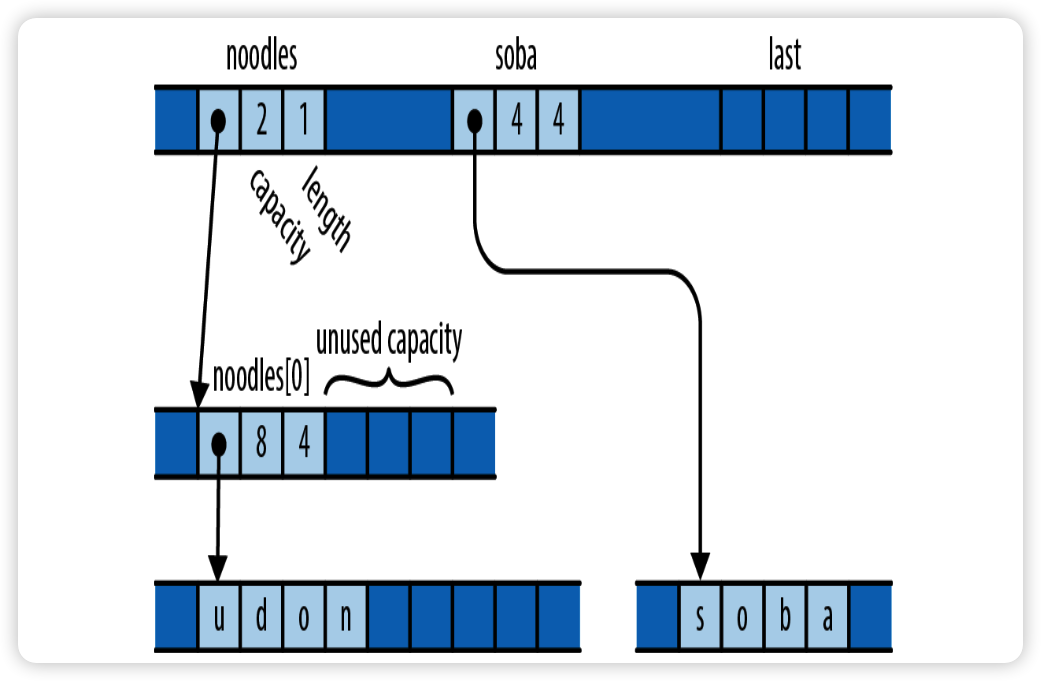
\includegraphics[width=0.8\textwidth]{../img/f22-3.png}
    \caption{一个有未初始化的空闲空间的vector}
    \label{f22-3}
\end{figure}

vector还有空闲的空间来存储另一个元素,但这块空间现在的值是无效的,可能是任何之前存在这里的值。假设再运行下面的代码:
\begin{minted}{Rust}
    noodles.push(soba);
\end{minted}

把字符串push进vector会把未初始化的内存转换为一个新的元素,如\autoref{f22-4}所示:
\begin{figure}[htbp]
    \centering
    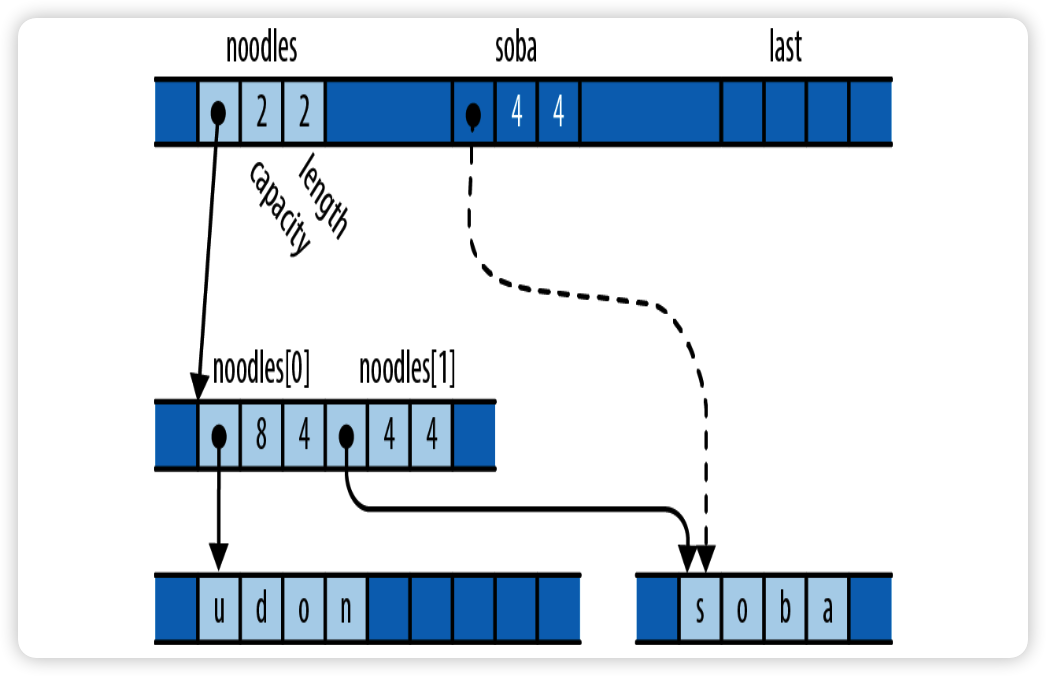
\includegraphics[width=0.8\textwidth]{../img/f22-4.png}
    \caption{把\texttt{soba}的值push进vector之后}
    \label{f22-4}
\end{figure}

vector初始化了空的空间,并且增大了长度来表示这是一个新的、还活着的元素。这个字符串的所有者现在变成了这个vector;你可以通过vector的第二个元素引用这个字符串,并且drop这个vector会释放这两个字符串。并且\texttt{soba}现在变为未初始化。

最后,如果从vector中弹出一个值:
\begin{minted}{Rust}
    last = noodles.pop().unwrap();
\end{minted}

在内存中,看起来像\autoref{f22-5}。
\begin{figure}[htbp]
    \centering
    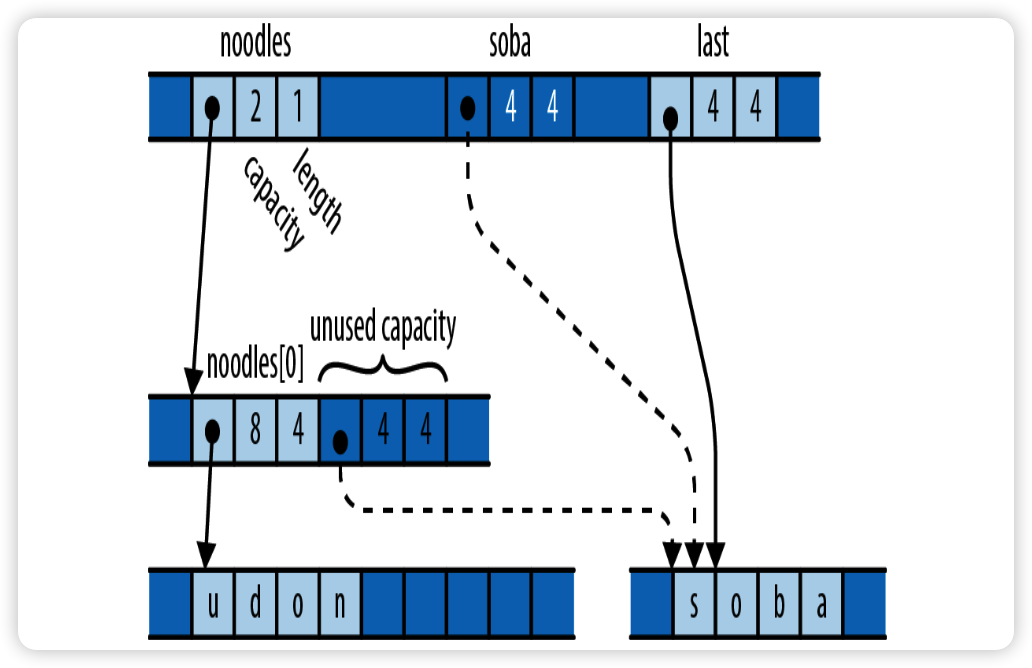
\includegraphics[width=0.8\textwidth]{../img/f22-5.png}
    \caption{从vector中弹出一个元素到\texttt{last}之后}
    \label{f22-5}
\end{figure}

变量\texttt{last}获得了字符串的所有权。vector减小了长度来表示用来存储字符串的空间现在变为未初始化。

和之前的\texttt{pot}和\texttt{pasta}一样,这里\texttt{soba}、\texttt{last}和vector的空闲空间可能有完全相同的比特位。但只有\texttt{last}被认为拥有这个值,认为另外两个位置有活着的值显然是错误的。

初始化过的值的真正定义是\emph{被认为是活着(treated as live)}的值。写入一个值的字节通常是初始化必要的步骤之一,但这只是因为这样做才能让值准备好被认为是活着的。move和copy在内存总的效果是一样的,区别在于move之后,源对象不再被认为是活着的,而copy之后,源对象和目标对象都是活着的。

Rust会在编译期追踪哪个局部变量是活着的,并阻止你使用那些值被移动走的变量。像\texttt{Vec}、\texttt{HashMap}、\texttt{Box}等类型都会动态追踪它们的缓冲区。如果你实现了一个自己管理内存的类,你需要做同样的事。

Rust为实现这样的类型提供了两个基本的操作:

\codeentry{std::ptr::read(src)}
\hangparagraph{从\texttt{src}指向的位置移出一个值,并把它的所有权交给调用者。\texttt{src}参数应该是一个\texttt{*const T}原始指针,其中\texttt{T}是一个sized类型。在调用这个函数之后,\texttt{*src}的内容不受影响,但除非\texttt{T}实现了\texttt{Copy},否则你必须保证你的程序不再把它们视为活着的值。}

\hangparagraph{这是\texttt{Vec::pop}背后的操作。pop一个值会调用\texttt{read}来把这个值移出缓冲区,然后减小长度来把这个空间标记为未初始化的。}

\codeentry{std::ptr::write(dest, value)}
\hangparagraph{把\texttt{value}移动到\texttt{dest}指向的位置,在调用之前\texttt{dest}指向的必须是未初始化的内存。引用物现在拥有这个值。\texttt{dest}必须是一个\texttt{*mut T}原始指针,\texttt{value}必须是一个\texttt{T}值,\texttt{T}是一个sized类型。}

\hangparagraph{这是\texttt{Vec::push}背后的操作。push一个值会调用\texttt{write}把值移动到下一个可用的位置,然后增大长度来表示这个位置现在是一个有效的元素。}

它们都是自由函数,不是原始指针类型的方法。

注意你不能对Rust的safe指针类型做这些操作,它们在任何时候都要求引用对象的时初始化过得,因此把一块未初始化的内存变为一个值,或者反过来,都超出了它们的能力。只有原始指针才符合要求。

标准库还提供了几个函数用来从一个内存块中把数组的值移动到另一个内存块中:

\codeentry{std::ptr::copy(src, dst, count)}
\hangparagraph{把内存中\texttt{src}位置开始的\texttt{count}个值移动到\texttt{dst}处,就好像你写了一个\texttt{read}和\texttt{write}调用的循环来一次一个地移动这些元素一样。目的位置在调用之前必须是未初始化的,调用之后源位置将是未初始化的。\texttt{src}和\texttt{dest}参数必须是\texttt{*const T}和\texttt{*mut T}原始指针,\texttt{count}必须是\texttt{usize}。}

\codeentry{ptr.copy\_to(dst, count)}
\hangparagraph{\texttt{copy}的一个更便利的版本,将从\texttt{ptr}开始处的\texttt{count}个值移动到\texttt{dst}位置处,不需要起始点作为参数。}

\codeentry{std::ptr::copy\_nonoverlapping(src, dst, count)}
\hangparagraph{类似于\texttt{copy},除了它的合约进一步要求源地址块和目的地址块不能重叠之外。它可能比\texttt{copy}快一点。}

\codeentry{ptr.copy\_to\_nonoverlapping(dst, count)}
\hangparagraph{\texttt{copy\_nonoverlapping}的一个更便利的版本,类似于\texttt{copy\_to}。}

\texttt{read}和\texttt{write}函数还有另外两个家族,也在\texttt{std::ptr}模块里:

\codeentry{read\_unaligned, write\_unaligned}
\hangparagraph{这两个函数类似于\texttt{read}和\texttt{write},除了不像通常的引用类型一样要求指针是对齐。这两个函数可能比普通的\texttt{read}和\texttt{write}函数。}

\codeentry{read\_volatile, write\_volatile}
\hangparagraph{这两个函数等价于C和C++中的volatile read和wirte。}

\subsection{示例:\texttt{GapBuffer}}
这里有一个简单的例子用到了刚才介绍的函数。

假设你正在编写一个文本编辑器,并且正在寻找一个类型来表示文本。你可以选择\texttt{String}并使用\texttt{insert}和\texttt{remove}方法来在用户打字时插入或删除字符。但如果他们正在编辑一个大文件的起始位置,这些方法的开销就会很大:插入一个字符需要在内存中向右移动右侧所有的字符,删除一个字符需要向左移动右侧的所有字符。你可能希望这样常用的操作开销能更小。

Emacs文本编辑器使用了一种叫做\emph{gap buffer}的简单数据结构,它可以在常量时间内插入和删除字符。\texttt{String}保持所有空闲空间都在文本的尾部,这样可以让\texttt{push}和\texttt{pop}操作的开销很小,而gap bufer把空闲空间保持在文本的中间,即正在编辑的地方。这样的空闲空间称为\emph{gap}。在gap处插入或删除元素的开销很小:只需要简单地缩写或者扩大gap。你只需要把gap一侧的文本移动到另一侧就可以把gap移动到任何位置。当gap为空时,可以迁移到一个更大的缓冲区。

尽管在gap buffer中插入和删除操作速度都很快,但改变正在编辑的位置需要把gap移动到一个新的位置。移动元素所需的时间和要移动的距离成正比。幸运的是,典型的编辑活动包括在缓冲区的某一区域进行大量的修改,然后再去其他位置操作文本。

在这一节中我们将用Rust实现一个gap buffer。为了避免被UTF-8干扰,我们用缓冲区直接存储\texttt{char}值,但即使以其他格式存储文本,操作的基本原则都是相同的。

首先,我们将用实践来展示一个gap buffer。这段代码创建了一个\texttt{GapBuffer},在其中插入了一些文本,然后把插入位置移动到最后一个单词之前:
\begin{minted}{Rust}
    let mut buf = GapBuffer::new();
    buf.insert_iter("Lord of the Rings".chars());
    buf.set_position(12);
\end{minted}

在运行过这段代码之后,缓冲区如\autoref{f22-6}所示。
\begin{figure}[htbp]
    \centering
    \includegraphics[width=0.9\textwidth]{../img/f22-6.png}
    \caption{一个包含一些文本的gap buffer}
    \label{f22-6}
\end{figure}

插入操作会用新的文本填充gap。这行代码添加了一个单词,破坏了现在的布局:
\begin{minted}{Rust}
    buf.insert_iter("Onion ".chars());
\end{minted}

结果如\autoref{f22-7}所示。

\begin{figure}[htbp]
    \centering
    \includegraphics[width=0.9\textwidth]{../img/f22-7.png}
    \caption{一个包含更多文本的gap buffer}
    \label{f22-7}
\end{figure}

这里是我们的\texttt{GapBuffer}类型:
\begin{minted}{Rust}
    use std;
    use std::ops::Range;

    pub struct GapBuffer<T> {
        // 存储元素。它提供我们需要的容量,但它的长度总是0。
        // GapBuffer把它的元素和gap放在`Vec`“未使用”的空间里。
        storage: Vec<T>,

        // `storage`中间未初始化的元素的范围。
        // 这个范围前面和后面的元素总是初始化过的。
        gap: Range<usize>
    }
\end{minted}

\texttt{GapBuffer}以一种奇怪的方式使用它的\texttt{storage}字段\footnote{还有一种方法可以更好地实现这些功能,这种方法需要使用编译器内部的\texttt{alloc} crate里的\texttt{RawVec}类型,不过这个crate仍然是unstable的。}。它永远不会真的在vector中存储任何元素。它只是简单的调用\texttt{Vec::with\_capacity(n)}来获得一个可以存储\texttt{n}个元素的足够大的内存块,通过vector的\texttt{as\_ptr}和\texttt{as\_mut\_ptr}方法获得指向内存块的原始指针,然后直接以它自己的方式来使用这块内存作为缓冲区。vector的长度将始终保持0.当\texttt{Vec}被drop时,\texttt{Vec}不会尝试释放它的元素,因为它不知道它持有任何元素,但它确实会释放这个内存块。这正是\texttt{GapBuffer}想要的;它有它自己的\texttt{Drop}实现,这个实现知道有效的元素在哪里并可以正确地drop它们。

\texttt{GapBuffer}的最简单的方法如你所料:
\begin{minted}{Rust}
    impl<T> GapBuffer<T> {
        pub fn new() -> GapBuffer<T> {
            GapBuffer { storage: Vec::new(), gap: 0..0 }
        }

        /// 返回这个GapBuffer在不重新分配的情况下可以存储的元素数量
        pub fn capacity(&self) -> usize {
            self.storage.capacity()
        }

        /// 返回这个GapBuffer当前持有的元素数量
        pub fn len(&self) -> usize {
            self.capacity() - self.gap.len()
        }

        /// 返回当前的插入位置
        pub fn position(&self) -> usize {
            self.gap.start
        }
        ...
    }
\end{minted}

它用了很多之前介绍的函数来实现一个方法,这个方法返回指向给定索引位置的元素的原始指针。在Rust里,我们需要一个\texttt{mut}指针的方法和一个\texttt{const}指针的方法。和上面的方法不同,它们并不是public的。继续这个\texttt{impl}块:
\begin{minted}{Rust}
    /// 返回一个指向底层存储中第`index`个元素的指针。不考虑gap。
    ///
    /// 安全性:`index`必须是`self.storage`中有效的索引
    unsafe fn space(&self, index: usize) -> *const T {
        self.storage.as_ptr().offset(index as isize)
    
    }

    /// 返回一个指向底层存储中第`index`个元素的可变指针。不考虑gap。
    ///
    /// 安全性:`index`必须是`self.storage`中有效的索引
    unsafe fn space_mut(&mut self, index: usize) -> *mut T {
        self.storage.as_mut_ptr().offset(index as isize)
    }
\end{minted}

为了查找给定索引处的元素,你必须考虑这个索引是落在gap之前还是之后,然后进行调整:
\begin{minted}{Rust}
    /// 返回第`index`个元素的偏移量,考虑gap。
    /// 这个函数并不检查index是否在范围内,
    /// 但它永远不会返回一个在gap中的位置
    fn index_to_raw(&self, index: usize) -> usize {
        if index.self.gap.start {
            index
        } else {
            index + self.gap.len()
        }
    }

    /// 返回第`index`个元素的引用,
    /// `index`超出范围时返回`None`
    pub fn get(&self, index: usize) -> Option<&T> {
        let raw = self.index_to_raw(index);
        if raw < self.capacity() {
            unsafe {
                // 我们已经检查过`raw`和`self.capacity()`的大小关系了,
                // 并且index_to_raw会跳过gap,因此这是安全的。
                Some(&*self.space(raw))
            }
        } else {
            None
        }
    }
\end{minted}

当我们开始在缓冲区中另一个位置开始插入或删除时,我们需要把gap移动到这个新位置。向右移动gap需要把元素向左移,反之亦然,就像水平仪中的液体流向一个方向时,气泡会向另一个方向移动:
\begin{minted}{Rust}
    /// 把当前的插入位置设置为`pos`。
    /// 如果`pos`越界就panic。
    pub fn set_position(&mut self, pos: usize) {
        if pos > self.len() {
            panic!("index {} out of range for GapBuffer", pos);
        }

        unsafe {
            let gap = self.gap.clone();
            if pos > gap.start {
                // `pos`落在了gap之后。通过把gap右侧的元素移动到`pos`之前
                // 来向右移动gap。
                let distance = pos - gap.start;
                std::ptr::copy(self.space(gap.end),
                               self.space_mut(gap.start),
                               distance);
            } else if pos < gap.start {
                // `pos`落在了gap之前。通过把gap左侧的元素移动到`pos`之后
                // 来向左移动gap。
                let distance = gap.start - pos;
                std::ptr::copy(self.space(pos),
                               self.space_mut(gap.end - distance),
                               distance);
            }

            self.gap = pos .. pos + gap.len();
        }
    }
\end{minted}

这个函数使用了\texttt{std::ptr::copy}方法来移动元素;\texttt{copy}要求目的位置必须是未初始化的,并且把源位置置为未初始化。源位置和目的位置可以重叠,\texttt{copy}会正确地处理这种情况。因为gap在这个调用之前是未初始化的内存,并且这个函数会调整gap的位置来覆盖那些copy移动走的元素,因此\texttt{copy}函数的合约得到了满足。

元素的插入和删除相对简单。插入操作从gap中拿出一个元素的空间来存储新元素,而删除操作把值移出并增大gap来覆盖空出来的空间:
\begin{minted}{Rust}
    /// 在当前的插入位置插入`elt`,
    /// 并把新的插入位置设置为`elt`之后。
    pub fn insert(&mut self, elt: T) {
        if self.gap.len() == 0 {
            self.enlarge_gap();
        }

        unsafe {
            let index = self.gap.start;
            std::ptr::write(self.space_mut(index), elt);
        }
        self.gap.start += 1;
    }


    /// 在当前的插入位置插入`iter`产生的元素,
    /// 并把新的插入位置设置为这些元素之后。
    pub fn insert_iter<I>(&mut self, iterable: I)
        where I: IntoIterator<Item=T>
    {
        for item in iterable {
            self.insert(item)
        }
    }

    /// 移除插入位置后的第一个元素并返回它,
    /// 如果插入位置是在GapBuffer的末尾则返回`None`
    pub fn remove(&mut self) -> Option<T> {
        if self.gap.end == self.capacity() {
            return None;
        }

        let element = unsafe {
            std::ptr::read(self.space(self.gap.end))
        };
        self.gap.end += 1;
        Some(element)
    }
\end{minted}

类似于\texttt{Vec}使用\texttt{std::ptr::write}来实现push、使用\texttt{std::ptr::read}来实现pop一样,\texttt{GapBuffer}使用\texttt{write}来实现\texttt{insert}、使用\texttt{read}来实现\texttt{remove}。并且就像\texttt{Vec}必须调整长度来维护已初始化元素和空闲空间的边界一样,\texttt{GapBuffer}也会调整它的gap。

当gap被填满时,\texttt{insert}方法必须增大缓冲区来获取更多的空闲空间。\texttt{enlarge\_gap}方法(\texttt{impl}块中的最后一个方法)用来实现这一点:
\begin{minted}{Rust}
    /// 把`self.storage`的容量翻倍
    fn enlarge_gap(&mut self) {
        let mut new_capacity = self.capacity() * 2;
        if new_capacity == 0 {
            // 如果现有的vector是空的,就选择一个合适的起始容量。
            new_capacity = 4;
        }

        // 我们不知道resize一个Vec会对它“未使用的空间进行什么操作。
        // 因此简单地创建一个新的vector并把元素移动过去。
        let mut new = Vec::with_capacity(new_capacity);
        let after_gap = self.capacity() - self.gap.end;
        let new_gap = self.gap.start .. new.capacity() - after_gap;

        unsafe {
            // 移动落在gap之前的元素。
            std::ptr::copy_nonoverlapping(self.space(0),
                                          new.as_mut_ptr(),
                                          self.gap.start);
            // 移动落在gap之后的元素。
            let new_gap_end = new.as_mut_ptr().offset(new_gap.end as isize);
            std::ptr::copy_nonoverlapping(self.space(self.gap.end),
                                          new_gap_end,
                                          after_gap);
        }

        // 这会释放旧的Vec,但不会drop任何元素,
        // 因为Vec的长度是0。
        self.storage = new;
        self.gap = new_gap;
    }
\end{minted}

和\texttt{set\_position}必须使用\texttt{copy}来移动元素不同,\texttt{enlarge\_gap}可以使用\texttt{copy\_nonoverlapping},因为它是把元素移动到一个完全全新的缓冲区。

把新的vector赋值给\texttt{self.storage}会drop旧的vector。但因为旧vector的长度是0,所以它会相信它没有要drop的元素,然后简单地释放缓冲区。\texttt{copy\_nonoverlapping}会让源地址变为未初始化的,所以旧vector的假设确实是正确的:现在所有的元素的所有权都在新vector里。

最后,我们需要确保drop一个\texttt{GapBuffer}会释放所有元素:
\begin{minted}{Rust}
    impl<T> Drop for GapBuffer<T> {
        fn drop(&mut self) {
            unsafe {
                for i in 0 .. self.gap.start {
                    std::ptr::drop_in_place(self.space_mut(i));
                }
                for i in self.gap.end .. self.capacity() {
                    std::ptr:;drop_in_place(self.space_mut(i));
                }
            }
        }
    }
\end{minted}

元素分布在gap之前和之后,因此我们迭代这两个区域并使用\texttt{std::ptr::drop\_in\_place}函数来drop每个元素。\texttt{drop\_in\_place}函数是一个工具函数,行为类似于\texttt{drop(std::ptr::read(ptr))},但不需要把值move给调用者(因此也可以用于unsized类型)。在\texttt{enlarge\_gap}中,当vector \texttt{self.storage}被drop时,它的缓冲区实际是未初始化的。

类似我们在本章中展示过的其他类型一样,\texttt{GapBuffer}确保它自己的不变量足够充分,以此来确保它用到的每个unsafe特性的合约都被遵守,因此它的所有public方法都不需要标记为unsafe。\texttt{GapBuffer}为一个在safe代码中不可能高效实现的特性实现了一个safe的接口。

\subsection{unsafe代码中的panic安全性}
在Rust中,panic通常不会导致未定义行为;\texttt{panic!}宏并不是一个unsafe特性。但当你决定在unsafe代码中使用它时,你就需要考虑panic安全性了。

考虑上一节定义的\texttt{GapBuffer::remove}方法:
\begin{minted}{Rust}
    pub fn remove(&mut self) -> Opton<T> {
        if self.gap.end == self.capacity() {
            return None;
        }
        let element = unsafe {
            std::ptr::read(self.space(self.gap.end))
        };
        self.gap.end += 1;
        Some(element)
    }
\end{minted}

\texttt{read}的调用会把元素立刻移出gap并留下未初始化的空间。这时\texttt{GapBuffer}处于一种不一致的状态:我们打破了所有gap之外的元素都必须是初始化过的这一不变量。幸运的是,下一条语句增大了gap让它覆盖了未初始化的空间,因此在我们返回时,不变量仍然成立。

但考虑如果在调用\texttt{read}之后、给\texttt{self.gap.end}赋值之前尝试使用一些可能panic的特性(例如索引元素)会发生什么。在这两个动作之间中断这个方法将会导致\texttt{GapBuffer}有一个未初始化的元素处于gap之外。下一次调用\texttt{remove}时将会再次尝试\texttt{read}这个元素;即使简单地drop \texttt{GapBuffer}也会尝试再次drop这个元素。这两种情况都是未定义行为,因为它们访问了未初始化的内存。

如果一个类型在方法里临时打破这个类型的不变量,然后再在返回之前恢复不变量,那么这个问题是不可避免的。在方法中途panic可能会缩短清理过程,让类型处于不一致的状态。

如果这个类型只使用safe代码,那么这种不一致可能会导致类型的行为出错,但不会导致未定义行为。但是用了unsafe特性的代码通常依赖它的不变量来满足那些特性的合约。被破坏的不变量会破坏合约,进而导致未定义行为。

当使用unsafe特性时,你必须特别注意那些临时打破不变量的区域,并保证它们不会在这些地方panic。



    \chapter{外部函数}\label{ch23}
\emph{Cyberspace. Unthinkable complexity. Lines of lightranged in the non-space of the mind, clusters andconstellations of data. Like city lights, receding . . .}

\begin{flushright}
    ——William Gibson, \emph{Neuromancer}
\end{flushright}

不幸的是,世界上不是每个程序都是用Rust编写的。我们可能想在我们的Rust程序中使用很多用其他语言实现的优秀的库和接口。Rust的\emph{外部语言接口(foreign function interface(FFI))}让Rust代码能调用C编写的函数和一部分C++编写的函数。因为大多数操作系统提供C接口,Rust的外部函数接口允许直接访问任何类型的底层设施。

在本章中,我们将编写一个链接到\texttt{libgit2}的程序,它是一个用于Git版本控制系统的C库。首先,我们将展示怎么直接在Rust中使用C函数,就使用我们上一章中介绍的unsafe特性。然后,我们将展示如何构建\texttt{libgit2}的safe接口,借助开源的\texttt{git2-rs} crate的灵感,这个crate正好实现了这一点。

我们将假设你熟悉C语言和编译链接C程序的机制。处理C++也相差不多。我们还假设你熟悉Git版本控制系统。

确实有Rust crate用于和很多其他语言例如Python、JavaScript、Lua和Java交互。我们没有足够的篇幅来介绍它们,但所有这些接口最终都是使用C外部函数接口实现的,因此无论你想和什么语言交互,这一章都能给你一个开头。

\section{寻找公共的数据表示}\label{repr}
Rust和C的公共基础是机器语言,因此为了预测Rust的值在C代码中看起来是什么样的,或者反过来,你需要考虑它们的机器级表示。在整本书中,我们一直着重展示一个值在内存中的实际表示,因此你可能已经注意到了C和Rust的数据世界有很多共通之处:例如Rust的\texttt{usize}和C的\texttt{size\_t}是相同的,两门语言中的结构体也基本相同。为了建立起Rust和C中相应类型的关系,我们将从基本类型开始,并逐渐扩展到更复杂的类型。

鉴于C主要用作系统编程,C中类型的表示总是令人惊讶的宽松:例如一个\texttt{int}通常是32位,但可能会更长,或者短到16位;一个C的\texttt{char}可能是有符号的也可能是无符号的。为了应对这种可变性,Rust的\texttt{std::os::raw}模块定义了一些Rust的类型,这些类型保证和相应的C类型有完全相同的表示(\hyperref[t23-1]{表23-1})。其中包括基本的整数和字符类型。

\begin{table}[htbp]
    \centering
    \caption{\texttt{std::os::raw}中的Rust类型}
    \label{t23-1}
    \begin{tabular}{ll}
        \textbf{C类型}  &   \textbf{相应的\texttt{std::os::raw}类型}    \\
        \hline
        \texttt{short}          &   \texttt{c\_short}   \\
        \rowcolor{tablecolor}
        \texttt{int}            &   \texttt{c\_int}     \\
        \texttt{long}           &   \texttt{c\_long}    \\
        \rowcolor{tablecolor}
        \texttt{long long}      &   \texttt{c\_longlong}    \\
        \texttt{unsigned short} &   \texttt{c\_ushort}  \\
        \rowcolor{tablecolor}
        \texttt{unsigned, unsigned int} &   \texttt{c\_uint}    \\
        \texttt{unsigned long}  &   \texttt{c\_ulong}   \\
        \rowcolor{tablecolor}
        \texttt{unsigned long long}     &   \texttt{c\_ulonglong}   \\
        \texttt{char}           &   \texttt{c\_char}    \\
        \rowcolor{tablecolor}
        \texttt{signed char}    &   \texttt{c\_schar}   \\
        \texttt{unsigned char}  &   \texttt{c\_uchar}   \\
        \rowcolor{tablecolor}
        \texttt{float}           &   \texttt{c\_float}    \\
        \texttt{double}         &   \texttt{c\_double}  \\
        \rowcolor{tablecolor}
        \texttt{void *, const void *}   &   \texttt{*mut c\_void, *const c\_void}   \\
    \end{tabular}
\end{table}

有关\hyperref[t23-1]{表23-1}的注意事项:
\begin{enumerate}
    \item 除了\texttt{c\_void}之外,这里所有的Rust类型都是某些基本Rust类型的别名:例如\texttt{c\_char}是\\
    \texttt{i8}或者\texttt{u8}。
    \item Rust的\texttt{bool}等价于C或C++的\texttt{bool}。
    \item Rust的32位\texttt{char}类型并不等同于\texttt{wchar\_t},后者的宽度和编码取决于具体实现。C的\texttt{char32\_t}倒是更接近一点,但它的编码仍然并不保证是Unicode。
    \item Rust的基础\texttt{usize}和\texttt{isize}类型和C的\texttt{size\_t}和\texttt{ptrdiff\_t}有相同的表示。
    \item C/C++指针和C++的引用对应Rust的原始指针类型\texttt{*mut T}和\texttt{*const T}。
    \item 从技术上讲,C标准允许实现使用一些Rust中没有相应类型的表示:36位整数、用符号+数字来表示有符号值等等。在实践中,在Rust被移植到的每个平台上,每个基本的C整数类型在Rust中都有对应的类型。
\end{enumerate}

为了定义兼容C结构体的Rust结构体类型,你可以使用\texttt{\#[repr(C)]}属性。在结构体的定义上面放上\texttt{\#[repr(C)]}可以要求Rust按照C编译器的方式放置结构体中的字段。例如,\texttt{libgit2}的\emph{git2/errors.h}头文件定义了下面的C结构体来提供一个错误的详情:
\begin{minted}{C}
    typedef struct {
        char *message;
        int klass;
    } git_error;
\end{minted}

你可以按照下面这样定义一个内存表示完全相同的Rust类型:
\begin{minted}{Rust}
    use std::os::raw::{c_char, c_int};

    #[repr(C)]
    pub struct git_error {
        pub message: *const c_char,
        pub klass: c_int
    }
\end{minted}

\texttt{\#[repr(C)]}属性只影响struct自身的布局,不会影响单个字段的表示,因此为了和C struct匹配,每一个字段也都要使用C风格的类型:例如用\texttt{*const c\_char}替换\texttt{char *},用\texttt{c\_int}替换\texttt{int}。

在这个特定的例子中,\texttt{\#[repr(C)]}属性可能并不会改变\texttt{git\_error}的布局。因为实际上没有那么多放置一个指针和一个整数的方法。但C和C++都保证一个结构体的成员按照声明的顺序依次在内存中排布,而Rust会按照总结构体大小最小的方式来组织字段,并且0大小的类型不占用空间。\texttt{\#[repr(C)]}属性告诉Rust按照C的规则来布局。

你也可以使用\texttt{\#[repr(C)]}来控制C风格的enum的表示:
\begin{minted}{Rust}
    #[repr(C)]
    #[allow(non_camel_case_types)]
    enum git_error_code {
        GIT_OK          = 0,
        GIT_ERROR       = -1,
        GIT_ENOTFOUND   = -3,
        GIT_EEXISTS     = -4,
        ...
    }
\end{minted}

通常情况下,Rust在选择如何表示enum时会使用各种技巧。例如,我们提到过Rust在一个单字中存储\texttt{Option<\&T>}(如果\texttt{T}是sized)。如果没有\texttt{\#[repr(C)]},Rust会使用单个字节来表示\texttt{git\_error\_code} enum;有了\texttt{\#[repr(C)]}之后,Rust会和C一样用一个C \texttt{int}一样大的值来存储。

你可以要求Rust使用和某些整数相同的表示来存储enum。上面的定义如果以\texttt{\#[repr(i16)]}\\
开头,将会得到一个和下面C++ enum相同的16位的表示:
\begin{minted}{C++}
    #include <stdint.h>

    enum git_error_code: int16_t {
        GIT_OK          = 0,
        GIT_ERROR       = -1,
        GIT_ENOTFOUND   = -3,
        GIT_EEXISTS     = -4,
        ...
    };
\end{minted}

正如之前提到的,\texttt{\#[repr(C)]}还可以用于union。\texttt{\#[repr(C)]} union的字段总是从union的内存的第一个位(0偏移处)开始。

假设你有一个C struct使用一个union来存储一些数据,再用一个tag值来指示应该使用union的哪个值,类似于Rust的enum一样:
\begin{minted}{C}
    enum tag {
        FLOAT = 0,
        INT   = 1,
    };

    union number {
        float f;
        short i;
    };

    struct tagged_number {
        tag t;
        number n;
    };
\end{minted}

Rust可以通过对enum、struct和union类型都应用\texttt{\#[repr(C)]}来实现一个这样的结构体,然后使用\texttt{match}语句基于tag来选择一个struct中的union的字段:
\begin{minted}{Rust}
    #[repr(C)]
    enum Tag {
        Float = 0,m
        Int   = 1
    }

    #[repr(C)]
    union FloatOrInt {
        f: f32,
        i: i32,
    }

    #[repr(C)]
    struct Value {
        tag: Tag,
        union: FloatOrInt
    }

    fn is_zero(v: Value) -> bool {
        use self::Tag::*;
        unsafe {
            match v {
                Value { tag: Int, union: FloatOrInt { i: 0 } } => true,
                Value { tag: Float, union: FloatOrInt { f: num } } => (num == 0.0),
                _ => false
            }
        }
    }
\end{minted}

使用这种技术,即使是复杂的结构体也可以很容易地跨FFI边界使用。

在Rust和C之间传递字符串要稍微更难一点。C使用一个空结尾的字符数组的指针来表示字符串。另一边Rust显式地存储字符串的长度,要么是\texttt{String}的一个字段,要么是一个胖引用\texttt{\&str}的第二个字。Rust的字符串不是空字符结尾的;事实上,它们的内容里可能包含空字符,这些空字符和其他字符一样,没有区别。

这意味着你不能借用一个Rust字符串来当做C字符串:如果你传给C代码一个Rust字符串的指针,它可能错误地把内容中一个空字符当做字符串的结尾,或者越界去查找一个不存在的结尾空字符。从另一个方向考虑,你也许可以借用一个C字符串作为一个Rust的\texttt{\&str},只要它的内容是有效的UTF-8。

这种情况强迫Rust必须把C的字符串看做和\texttt{String}、\texttt{\&str}完全不同的类型。在\texttt{std::ffi}模块中,\texttt{CString}和\texttt{CStr}类型表示拥有所有权的和借用的空字符结尾的字节数组。和\texttt{String}、\texttt{str}比起来,\texttt{CString}和\texttt{CStr}的方法非常有限,基本只有构建自身和转换成其他类型的方法。我们将在下一节中用实例展示这些类型。

\section{声明外部函数和变量}
用\texttt{extern}块来声明其他库中定义的函数和变量,最终的Rust编译出的可执行文件会链接到这些库。例如,在大多数平台上,每个Rust程序都会链接到标准的C库,因此我们可以像这样告诉Rust C库里的\texttt{strlen}函数:
\begin{minted}{Rust}
    use std::os::raw::c_char;

    extern {
        fn strlen(s: *const c_char) -> usize;
    }
\end{minted}

这样就告诉了Rust这个函数的名字和类型,定义将会在之后进行链接。

Rust假设在\texttt{extern}块中声明的函数使用C语言的惯例来传递参数和接受返回值。它们被定义为\texttt{unsafe}函数。对\texttt{strlen}来说,这是正确的选择:它实际上是一个C函数,它的C规范要求你传入一个有效的以空字符结尾的字符串指针,而这是一个Rust无法强制的合约。(几乎任何接受原始指针作为参数的函数都必须是\texttt{unsafe}的:safe Rust可以从任何整数构造原始指针,但解引用这样的指针可能会导致未定义行为。)

有了这个\texttt{extern}块,我们可以像任何其他Rust函数一样调用\texttt{strlen},尽管它的类型显示了它是别的语言中定义的函数:
\begin{minted}{Rust}
    use std::ffi::CString;

    let rust_str = "I'll be back";
    let null_terminated = CString::new(rust_str).unwrap();
    unsafe {
        assert_eq!(strlen(null_terminated.as_ptr()), 12);
    }
\end{minted}

\texttt{CString::new}函数构建出一个空字符结尾的C字符串。它首先检查它的内容里是否有空字符,因为如果有空字符就不能用C字符串来表示它,如果找到了空字符就返回一个error(因此需要调用\texttt{unwrap})。否则,它向结尾添加一个空字符并返回一个\texttt{CString},这个\texttt{CString}持有最后的字符的所有权。

\texttt{CString::new}的开销取决于参数的类型。它接受任何实现了\texttt{Into<Vec<u8>>}的类型,传递一个\texttt{\&str}需要一次内存分配和拷贝,因为它到\texttt{Vec<u8>}的转换需要在堆上构建一份字符串的拷贝,这样vector才能拥有字符串的所有权。但以值传递一个\texttt{String}简单地消耗掉这个字符串并获取它的缓冲区的所有权,因此除非向缓冲区中添加一个空字符需要扩大缓冲区,否则这个转换完全不需要拷贝文本或内存分配。

\texttt{CString}解引用到\texttt{CStr},后者的\texttt{as\_ptr}方法返回一个\texttt{*const c\_char}指向字符串的头部。这正是\texttt{strlen}期望的类型。在这个例子中,\texttt{strlen}遍历字符串,寻找\texttt{CString::new}添加的空字符,然后返回字符串的长度,即字节数。

你也可以在\texttt{extern}块中声明全局变量,POSIX系统有一个叫做\texttt{environ}的全局变量存储进程的环境变量。在C中,它被声明为:
\begin{minted}{Rust}
    extern char **environ;
\end{minted}

在Rust中,你可以写:
\begin{minted}{Rust}
    use std::ffi::CStr;
    ues std::os::raw::c_char;

    extern {
        static environ: *mut *mut c_char;
    }
\end{minted}

为了打印出环境变量的第一个元素,你可以写:
\begin{minted}{Rust}
    unsafe {
        if !environ.is_null() && !(*environ).is_null() {
            let var = CStr::from_ptr(*environ);
            println!("first environment variable: {}",
                     var.to_string_lossy())
        }
    }
\end{minted}

在确保了\texttt{environ}有第一个元素之后,代码调用了\texttt{CStr::from\_ptr}来构建一个借用它的\texttt{CStr}。\texttt{to\_string\_lossy}方法返回一个\texttt{Cow<str>}:如果C字符串包含有效的UTF-8,\texttt{Cow}会以\texttt{\&str}的形式借用它的内容,不包括结尾的空字符。否则,\texttt{to\_string\_lossy}在堆上构造一份文本的拷贝,把其中非UTF-8的字符序列替换为官方的Unicode替换字符�,并构造出一个拥有它所有权的\texttt{Cow}。无论是哪种情况,结果都实现了\texttt{Display},因此你可以使用\texttt{\{\}}格式化参数打印出它。

\section{使用库里的函数}
为了使用一个特定的库提供的函数,你可以在\texttt{extern}块上方加上\texttt{\#[link]}属性来指定Rust应该链接的库的名称。例如,这里有一个程序调用\texttt{libgit2}的初始化和结束函数,但不做任何其他事:
\begin{minted}{Rust}
    use std::os::raw::c_int;

    #[link(name = "git2")]
    extern {
        pub fn git_libgit2_init() -> c_int;
        pub fn git_libgit2_shutdown() -> c_int;
    }

    fn main() {
        unsafe {
            git_libgit2_init();
            git_libgit2_shutdown();
        }
    }
\end{minted}

\texttt{extern}和之前一样声明了外部函数。\texttt{\#[link(name = "git2")]}属性会要求当Rust创建最终的可执行文件或者共享库时,它应该链接到\texttt{git2}库。Rust使用系统的链接器来构建可执行文件:在Unix上,它会向链接器的命令行传递\texttt{-lgit2}参数;在Windows上,它会传递\texttt{git2.LIB}参数。

\texttt{\#[link]}属性在库crate中也可以工作。当你构建一个依赖其他crate的程序时,Cargo会从整个依赖图中抓取所有链接项并在最后的链接中全部加进去。

如果你想要在你自己的机器上继续这个例子,你需要自己构建\texttt{libgit2}。我们使用\href{https://libgit2.org/}{libgit2} 0.25.1版本。为了编译\texttt{libgit2},你需要安装CMake构建工具和Python;我们使用了\href{https://cmake.org/}{CMake} 3.8.0版本和\href{https://www.python.org/}{Python} 2.7.13版本。

构建\texttt{libgit2}的完整文档可以在网站上找到,但因为非常简单所以我们将在这里展示基本的一些步骤。在Linux上,假设你已经把库的源码解压到了目录\emph{/home/jimb/libgit2-0.25.1}:
\begin{minted}{bash}
    $ cd /home/jimb/libgit2-0.25.1
    $ mkdir build
    $ cd build
    $ cmake ..
    $ cmake --build .
\end{minted}

在Linux上,这会生成一个共享库\emph{/home/jimb/libgit2-0.25.1/build/libgit2.so.0.25.1},还有一些指向它的符号链接,包括有一个叫\emph{libgit2.so}的。在macOS上,结果与此类似,但库的名字叫\emph{libgit2.dylib}。

在Windows上也非常简单。假设你把源码解压到了目录\emph{C:\textbackslash{}Users\textbackslash{}JimB\textbackslash{}libgit2-0.25.1}。在一个Visual Studio的命令提示符中:
\begin{minted}{PowerShell}
    > cd C:\Users\JimB\libgit2-0.25.1
    > mkdir build
    > cd build
    > cmake -A x64 ..
    > cmake --build .
\end{minted}

这些命令和在Linux上用的命令几乎一样,除了在第一次运行CMake的时候必须指定64位的构建来匹配你的Rust编译器。(如果你安装了32位的Rust工具链,那么你应该省略第一条\texttt{cmake}命令的\texttt{-A x64}标记。)这会产生一个导入库\emph{git2.LIB}和一个动态链接库\emph{git2.DLL},都在目录\emph{C:\textbackslash{}Users\textbackslash{}JimB\textbackslash{}libgit2-0.25.1\textbackslash{}build\textbackslash{}Debug}。(之后的命令都是以Unix为例,如果Windows上的命令大不相同的话会再加上Windows上的命令。)

在一个单独的目录里创建Rust程序:
\begin{minted}{bash}
    $ cd /home/jimb
    $ cargo new --bin git-toy
         Created binary (application) `git-toy` package
\end{minted}

复制我们之前展示的代码并粘贴到\emph{src/main.rs}里。当然,如果你尝试构建,Rust会不知道在哪查找你构建的\texttt{libgit2}库:
\begin{minted}{text}
    $ cd git-toy
    $ cargo run
       Compiling git-toy v0.1.0 (/home/jimb/git-toy)
    error: linking with `cc` failed: exit code: 1
       |
       = note: /usr/bin/ld: error: cannot find -lgit2
               src/main.rs:11: error: undefined reference to 'git_libgit2_init'
               src/main.rs:12: error: undefined reference to 'git_libgit2_shutdown'
               collect2: error: ld returned 1 exit status
    
    error: aborting due to previous error
    error: could not complie `git-toy`
    To learn more, run the command again with --verbose.
\end{minted}

你可以通过编写一个\emph{构建脚本}来告诉Rust在哪搜索这个库,构建脚本是Cargo会在编译期编译并运行的Rust代码。构建脚本可以做很多事:动态生成代码,编译要被包含在crate中的C代码等等。在这个例子中,你需要做的只是向可执行文件的链接命令中添加一个库的搜索路径。当Cargo运行构建脚本时,它会解析构建脚本的输出来获取这类信息,因此构建脚本只需要把正确的信息打印到标准输出就可以了。

为了创建你自己的构建脚本,在\emph{Cargo.toml}所在的目录下添加一个叫\emph{build.rs}的文件,内容如下:
\begin{minted}{Rust}
    fn main() {
        println!(r"cargo:rustc-link-search=native=/home/jimb/libgit2-0.25.1/build");
    }
\end{minted}

这是Linux上的正确路径;在Windows上,你应该把\texttt{native=}之后的路径替换为\\
\emph{C:\textbackslash{}Users\textbackslash{}JimB\textbackslash{}libgit2-0.25.1\textbackslash{}build\textbackslash{}Debug}。(我们忽略了一些细节来保证这个例子的简洁;在一个真实的应用中,你应该避免在构建脚本中使用绝对路径。我们在本节结尾给出了如何正确实现这一点的文档。)

现在你基本上可以运行这个程序了。在macOS上它可能可以立即工作;但在Linux系统上你可能会看到类似这样的输出:
\begin{minted}{text}
    $ cargo run
       Compiling git-toy v0.1.0 (/tmp/rustbook-transcript-tests/git-toy)
        Finished dev [unoptimized + debuginfo] target(s)
         Running `target/debug/git-toy`
    target/debug/git-toy: error while loading shared libraries: libgit2.so.25: cannot open shared object file:
    no such file or directory
\end{minted}

意思是说,尽管Cargo成功地把可执行文件链接到了库,但它不知道怎么在运行时找到共享库。在Windows上通过弹出一个对话框来报告这个错误。在Linux上,你必须设置\texttt{LD\_LIBRARY\_PATH}环境变量:
\begin{minted}{bash}
    $ export LD_LIBRARY_PATH=/home/jimb/libgit2-0.25.1/build:$LD_LIBRARY_PATH
    $ cargo run
        Finished dev [unoptimized + debuginfo] target(s) in 0.0 secs
         Running `target/debug/git-toy`
\end{minted}

在macOS上,你可能需要设置\texttt{DYLD\_LIBRARY\_PATH}。

在Windows上,你必须设置\texttt{PATH}环境变量:
\begin{minted}{PowerShell}
    > set PATH=C:\Users\JimB\libgit2-0.25.1\build\Debug;%PATH%
    > cargo run
        Finished dev [unoptimized + debuginfo] target(s) in 0.0 secs
         Running `target/debug/git-toy`
    >
\end{minted}

当然,在一个要部署的应用中你可能想避免只为了寻找你的库而修改环境变量。一种替代方案是把C库静态链接到你的crate里。这会把库的目标文件拷贝到crate的\emph{.rlib}文件里,和这个crate中的Rust代码生成的目标文件和元数据放在一起。然后这整个集合会参与最终的链接。

Cargo的一个惯例是提供C库访问的crate应该命名为\texttt{LIB-sys},其中\texttt{LIB}是C库的名称。一个\texttt{-sys} crate应该只包含静态链接的库和包含\texttt{extern}块和类型定义的Rust模块。更高层的接口应该应该在依赖\texttt{-sys} crate的crate中实现。这允许多个上游的crate依赖同一个\texttt{-sys} crate,假设有一个版本的\texttt{-sys} crate可以满足每个上游的需要的话。

有关Cargo的构建脚本和与系统库的链接的完整文档见\href{https://doc.rust-lang.org/cargo/reference/build-scripts.html}{在线Cargo文档}。它展示了如何在构建脚本中避免绝对路径、控制编译选项、使用例如\texttt{pkg-config}的工具,等等。\texttt{git2-rs} crate也提供了模仿的好例子,它的构建脚本处理了一些很复杂的情况。

\section{一个libgit2的原始接口}
如何正确地使用\texttt{libgit2}可以分解为两个问题:
\begin{enumerate}
    \item 如何在Rust中使用\texttt{libgit2}的函数?
    \item 如何通过它们构建一个safe Rust的接口?
\end{enumerate}

我们将逐一解决这两个问题。在本节中,我们将编写一个程序,它基本上是一个巨大的\texttt{unsafe}块,充满了不规范的Rust代码,它反映了类型系统和惯例的冲突,这也是混合语言编程所固有的特点。我们称其为\emph{原始(raw)}接口。它的代码可能有些凌乱,但它能展示出Rust代码使用\texttt{libgit2}时必须的所有步骤。

然后,在下一节中,我们将构建一个\texttt{libgit2}的safe接口,它使用Rust的类型来强迫\emph{libgit2}对使用者隐含的要求。幸运的是,\texttt{libgit2}是一个设计得非常好的C库,因此Rust的安全性要求的问题都有很好的答案,并且我们可以构建出没有\texttt{unsafe}函数的规范的Rust接口。

我们要写的程序非常简单:它以命令行参数的形式接受一个路径,打开那里的Git仓库,然后打印出head commit的信息。但这足以用来展示构建safe和规范的Rust接口的关键策略。

对于原始接口,程序需要很多\texttt{libgit2}中的函数和类型,因此把\texttt{extern}块移动到它自己的模块是有意义的。我们将在\emph{git-toy/src}中创建一个叫\emph{raw.rs}的文件,内容如下:
\begin{minted}{Rust}
    #![allow(non_camel_case_types)]

    use std::os::raw::{c_int, c_char, c_uchar};

    #[link(name = "git2")]
    extern {
        pub fn git_libgit2_init() -> c_int;
        pub fn git_libgit2_shutdown() -> c_int;
        pub fn giterr_last() -> *const git_error;

        pub fn git_repository_open(out: *mut *mut git_repository,
                                   path: *const c_char) -> c_int;
        
        pub fn git_repository_free(repo: *mut git_repository);
        
        pub fn git_reference_name_to_id(out: *mut git_oid,
                                        repo: *mut git_repository,
                                        reference: *const c_char) -> c_int;
        
        pub fn git_commit_lookup(out: *mut *mut git_commit,
                                 repo: *mut git_repository,
                                 id: *const git_oid) -> c_int;

        pub fn git_commit_author(commit: *const git_commit) -> *const git_signature;
        pub fn git_commit_message(commit: *const git_commit) -> *cosnt c_char;
        pub fn git_commit_free(commit: *mut git_commit);
    }

    #[repr(C)] pub struct git_repository { _private: [u8; 0] }
    #[repr(C)] pub struct git_commit { _private: [u8; 0] }

    #[repr(C)]
    pub struct git_error {
        pub message: *const c_char,
        pub klass: c_int
    }

    pub const GIT_OID_RAWSZ: usize = 20;

    #[repr(C)]
    pub struct git_oid {
        pub id: [c_uchar; GIT_OID_RAWSZ]
    }

    pub type git_time_t = i64;

    #[repr(C)]
    pub struct git_time {
        pub time: git_time_t,
        pub offset: c_int
    }

    #[repr(C)]
    pub struct git_signature {
        pub name: *const c_char,
        pub email: *const c_char,
        pub when: git_time
    }
\end{minted}

其中每一项都是根据\texttt{libgit2}的头文件来声明的。例如\\
\emph{libgit2-0.25.1/include/git2/repository.h}中包含这个声明:
\begin{minted}{C}
    extern int git_repository_open(git_repository **out, const char *path);
\end{minted}

这个函数尝试打开\texttt{path}处的Git仓库。如果一切顺利,它会创建一个\texttt{git\_repository}对象并把该对象的指针存储在\texttt{out}指向的位置。等价的Rust声明如下:
\begin{minted}{Rust}
    pub fn git_repository_open(out: *mut *mut git_repository,
                               path: *const c_char) -> c_int;
\end{minted}

\texttt{libgit2} public的头文件使用typedef定义了一个不完全的\texttt{git\_repository}类型:
\begin{minted}{C}
    typedef struct git_repository git_repository;
\end{minted}

因为这个类型的详情是private的,因此public的头文件中并没有定义\\
\texttt{struct git\_repository},以确保库的使用者永远不能自己构造这个类型的实例。在Rust中一种可行的定义不完全的struct类型的方法是:
\begin{minted}{Rust}
    #[repr(C)] pub struct git_repository { _private: [u8; 0] }
\end{minted}

这个struct类型包含一个没有元素的数组。因为\texttt{\_private}字段不是\texttt{pub}的,所以不能在这个模块之外构造这个类型的值,正好对应了\texttt{libgit2}中不应该手动构造的类型。这种类型只能通过原始指针来进行操作。

手动编写一个巨大的\texttt{extern}块可能会很繁琐。如果你正在编写一个复杂的C库的Rust接口,你可能会想尝试\texttt{bindgen} crate,它包含一些可以在构建脚本中使用的函数,这些函数可以解析C头文件并自动生成相应的Rust声明。这里我们没有篇幅去介绍\texttt{bindgen},但\href{https://crates.io/crates/bindgen}{crates.io上的\texttt{bindgen}的页面}包含了它的文档的链接。

接下来我们将完全重写\emph{main.rs}。首先,我们需要声明\texttt{raw}模块:
\begin{minted}{Rust}
    mod raw;
\end{minted}

根据\texttt{libgit2}的惯例,可能失败的函数会返回一个整数码,成功时整数码为正数或者0,失败时整数码为负数。如果有错误发生,\texttt{giterr\_last}函数将会返回一个\texttt{git\_error}结构体的指针,这个结构体会提供更多有关错误的细节。\texttt{libgit2}持有这个结构体,所以我们不需要自己free它,但它可能被后续的调用覆盖。一个恰当的Rust接口应该使用\texttt{Result},但是在原始的版本中,我们将按照\texttt{libgit2}的方式使用它的函数,因此我们将编写我们自己的函数来处理错误:
\begin{minted}{Rust}
    use std::ffi::CStr;
    use std::os::raw::c_int;

    fn check(activity: &'static str, status: c_int) -> c_int {
        if status < 0 {
            unsafe {
                let error = &*raw::giterr_last();
                println!("error while {}: {} ({})", activity,
                         CStr::from_ptr(error.message).to_string_lossy(),
                         error.klass);
                std::process::exit(1);
            }
        }
        status
    }
\end{minted}

我们将使用这个函数检查\texttt{libgit2}调用的结果:
\begin{minted}{Rust}
    check("initializing library", raw::git_libgit2_init());
\end{minted}

这里使用了之前用过的\texttt{CStr}的方法:使用\texttt{from\_ptr}来从C字符串构造一个\texttt{CStr},使用\texttt{to\_string\_lossy}来把它转换成Rust可以打印的类型。

接下来,我们需要一个函数来打印出一次commit:
\begin{minted}{Rust}
    unsafe fn show_commit(commit: *const raw::git_commit) {
        let author = raw::git_commit_author(commit);

        let name = CStr::from_ptr((*author).name).to_string_lossy();
        let email = CStr::from_ptr((*author).email).to_string_lossy();
        println!("{} <{}>\n", name, email);

        let message = raw::git_commit_message(commit);
        println!("{}", CStr::from_ptr(message).to_string_lossy());
    }
\end{minted}

给定一个\texttt{git\_commit}的指针,\texttt{show\_commit}会调用\texttt{git\_commit\_author}和\\
\texttt{git\_commit\_message}来获取它需要的信息。这两个函数遵循了\texttt{libgit2}在文档中解释的一个惯例:

\emph{如果一个函数返回一个对象作为返回值,那个这个函数是一个getter,并且对象的生命周期被绑定到父对象上。}

用Rust的术语来说就是,\texttt{author}和\texttt{message}是从\texttt{commit}的借用,所以\texttt{show\_commit}不需要自己释放它们,但它绝对不能在\texttt{commit}被释放之后仍然持有它们。因为这个API使用了原始指针,所以Rust不会为我们检查它们的生命周期:如果我们意外地创建了悬垂指针,可能直到程序崩溃时我们才会发现。

上面的代码假设这些字段都持有UTF-8文本,但这个假设并不总是正确的。Git也允许其他的编码。正确地解析这些字符串可能需要使用\texttt{encoding} crate。为了保持简洁,我们在这里忽略这些问题。

我们程序的\texttt{main}函数如下:
\begin{minted}{Rust}
    use std::ffi::CString;
    use std::mem;
    use std::ptr;
    use std::os::raw::c_char;

    fn main() {
        let path = std::env::args().skip(1).next()
            .expect("usage: git-toy PATH");
        let path = CString::new(path)
            .expect("path contains null characters");

        unsafe {
            check("initializing library", raw::git_libgit2_init());

            let mut repo = ptr::null_mut();
            check("opening repository",
                  raw::git_repository_open(&mut repo, path.as_ptr()));
                
            let c_name = b"HEAD\0".as_ptr() as *const c_char;
            let oid = {
                let mut oid = mem::MaybeUninit::uninit();
                check("looking up HEAD",
                      raw::git_reference_name_to_id(oid.as_mut_ptr(), repo, c_name));
                oid.assume_init()
            };

            let mut commit = ptr::null_mut();
            check("looking up commit",
                  raw::git_commit_lookup(&mut commit, repo, &oid));
            
            show_commit(commit);

            raw::git_commit_free(commit);

            raw::git_repository_free(repo);

            check("shutting down library", raw::git_libgit2_shutdown);
        }
    }
\end{minted}

这段代码首先处理path参数并初始化库,都是我们之前见过的内容。第一行有趣的代码是:
\begin{minted}{Rust}
    let mut repo = ptr::null_mut();
    check("opening repository",
          raw::git_repository_open(&mut repo, path.as_ptr()));
\end{minted}

对\texttt{git\_repository\_open}的调用会尝试在打开指定路径的Git仓库。如果它成功了,它会分配一个新的\texttt{git\_repository}对象并设置\texttt{repo}指向它。Rust隐式把引用转换成原始指针,因此这里传递的\texttt{\&mut repo}提供了调用所需的\texttt{*mut *mut git\_repository}参数。

这里展示了另一个\texttt{libgit2}在使用中的惯例(摘自\texttt{libgit2}的文档):

\emph{以指针的指针形式的第一个参数返回的对象由调用者持有,调用者负责释放它们。}

用Rust的术语来说就是,像\texttt{git\_repository\_open}这样的函数会把新值传递给调用者。

接下来,考虑查找仓库当前head commit的对象哈希值的代码:
\begin{minted}{Rust}
    let oid = {
        let mut oid = mem::MaybeUninit::uninit();
        check("looking up HEAD",
              raw::git_reference_name_to_id(oid.as_mut_ptr(), repo, c_name));
        oid.assume_init()
    };
\end{minted}

\texttt{git\_oid}类型存储了一个对象的标识符——Git内部使用的一个160位的哈希值,Git使用它来识别commit、文件的不同版本,等等。对\texttt{git\_reference\_name\_to\_id}的调用会查找当前\texttt{"HEAD"} commit的对象标识符。

在C语言中向函数传递一个指针,然后在函数里填充指针指向对象的值是一种非常常用的初始化变量的方法,\texttt{git\_reference\_name\_to\_id}的第一个参数也是这样的。但是Rust不允许我们借用一个未初始化变量的引用。我们可以用0值初始化\texttt{oid},但这是一种浪费:因为之后存储在这里的值都会被覆盖。

要求Rust给我们未初始化的内存是可行的,但因为在任何时刻读取未初始化的内存都是未定义行为,因此Rust提供了一个抽象\texttt{MaybeUninit}来方便使用。\texttt{MaybeUninit<T>}告诉编译器为你的类型\texttt{T}分配足够的内存空间,但并不能访问这块空间,直到你声明现在已经可以安全地访问了。当这块内存的所有权属于\texttt{MaybeUninit}时,编译器也可以避免一些可能会导致未定义行为的特殊优化,否则即使你没有在代码中显式地访问未初始化的内存,这些优化也可能导致未定义行为。

\texttt{MaybeUninit}提供了一个方法\texttt{as\_mut\_ptr()},它产生一个指向它持有的未初始化内存的\texttt{*mut T}指针。把这个指针传给用于初始化内存的外部函数,然后调用\texttt{MaybeUninit}的unsafe\\
的\texttt{assume\_init}方法来产生一个完全初始化过的\texttt{T}。这样既不会有先初始化后立刻重新初始化的开销,也可以避免未定义行为。\texttt{assume\_init}是unsafe的,因为如果在并没有正确初始化的内存上调用它会立刻导致未定义行为。

在这个例子中是安全的,因为\texttt{git\_reference\_name\_to\_id}会初始化\texttt{MaybeUninit}拥有的内存。我们也可以将\texttt{MaybeUninit}用于\texttt{repo}和\texttt{commit}变量,但因为它们只是单个字,所以我们只是直接将它们初始化为空:
\begin{minted}{Rust}
    let mut commit = ptr::null_mut();
    check("looking up commit",
          raw::git_commit_lookup(&mut commit, repo, &oid));
\end{minted}

这里接受commit的对象标识符然后查找commit,成功时把一个\texttt{git\_commit}对象的指针存储在\texttt{commit}中。

\texttt{main}函数的其他部分应该是不言自明的。它调用了之前定义的\texttt{show\_commit}函数,然后释放了commit和repository对象,最后关闭了库。

现在我们可以在任何Git仓库上尝试我们的程序:
\begin{minted}{text}
    $ cargo run /home/jimb/rbattle
        Finished dev [unoptimized + debuginfo] target(s) in 0.0 secs
         Running `target/debug/git-toy /home/jimb/rbattle`
    Jim Blandy <jimb@red-bean.com>

    Animate goop a bit.
\end{minted}

\section{一个libgit2的安全接口}\label{SafeInter}
\texttt{libgit2}的原始接口是一个unsafe特性的完美示例:它完全可以被正确地使用(正如我们在这里所做的一样),但Rust不能强迫这些你必须遵守的规则。为一个类似这样的库设置一个safe的API的主要问题是识别所有这些规则,然后将所有违反规则的行为转换为违反借用后检查的错误。

这里是程序使用到的\texttt{libgit2}的特性的规则:
\begin{enumerate}
    \item 在调用库中任何其他函数之前,你必须先调用\texttt{git\_libgit2\_init}。在调用\\
    \texttt{git\_libgit2\_shutdown}之后你不能再调用库中任何一个函数。
    \item 除了输出参数之外,传递给\texttt{libgit2}函数的所有值必须是必须是完全初始化的。
    \item 当一次调用失败时,用来存储调用结果的输出参数仍然保持未初始化,你绝对不能使用它的值。
    \item 一个\texttt{git\_commit}对象引用了派生它的\texttt{git\_repository}对象,因此前者的生命周期绝对不能比后者长。(这一点并没有在\texttt{libgit2}的文档中说明;我们根据接口中的某些函数的存在推断出这一点,并通过阅读源码证实了它。)
    \item 类似的,一个\texttt{git\_signature}也总是借用自一个给定的\texttt{git\_commit},因此前者的生命周期绝对不能比后者长。(文档并没有覆盖这一点。)
    \item 一个commit关联的message和author的name和email总是借用自commit,因此绝对不能在commit被free之后再使用它们。
    \item 一旦一个\texttt{libgit2}对象被释放之后,绝不能再次使用它。
\end{enumerate}

事实证明,你可以构建出一个强迫所有这些规则的\texttt{libgit2}的Rust接口,可能是通过Rust的类型系统,也可能是通过内部管理细节。

在我们开始之前,让我们重新组织一下这个项目。我们希望有一个\texttt{git}模块用来导出safe的接口,之前的程序中的原始接口作为一个private的子模块。

整个源码树看起来像这样:
\begin{minted}{text}
    git-toy/
    |-- Cargo.toml
    |-- build.rs
    |-- src/
        |-- main.rs
        |-- git/
            |-- mod.rs
            |-- raw.rs
\end{minted}

按照我们在\nameref{ModInFile}中介绍过的规则,\texttt{git}模块的源码应该在\emph{git/mod.rs},\texttt{git::raw}子模块的源码应该在\emph{git/raw.rs}。

我们将完全重写\emph{main.rs}。它应该以\texttt{git}模块的声明开始:
\begin{minted}{Rust}
    mod git;
\end{minted}

然后,我们将需要创建\emph{git}子目录并把\emph{raw.rs}移动进去:
\begin{minted}{bash}
    $ cd /home/jimb/git-toy
    $ mkdir src/git
    $ mv src/raw.rs src/git/raw.rs
\end{minted}

\texttt{git}模块需要声明它的\texttt{raw}子模块。文件\emph{src/git/mod.rs}必须声明:
\begin{minted}{Rust}
    mod raw;
\end{minted}

因为它不是\texttt{pub}的,所以这个子模块对主程序不可见。

另外我们将需要使用一些\texttt{libc} crate里的函数,因此我们必须在\emph{Cargo.toml}中添加依赖。现在这个文件完整的内容是:
\begin{minted}{toml}
    [package]
    name = "git-toy"
    version = "0.1.0"
    authors = ["You <you@example.com>"]
    edition = "2018"

    [dependencies]
    libc = "0.2"
\end{minted}

现在我们已经重新组织了我们的模块,让我们来考虑下错误处理。就连\texttt{libgit2}的初始化函数都可能返回一个错误码,因此我们必须在准备开始之前准备好这一点。一个规范的Rust接口需要自己的\texttt{Error}类型,它需要捕获\texttt{libgit2}的错误码和来自\texttt{giterr\_last}的错误类型和消息。一个正确的错误类型必须实现通常的\texttt{Error}、\texttt{Debug}和\texttt{Display} trait。然后,它需要自己的\texttt{Result}类型来使用这个\texttt{Error}类型。这里是\emph{src/git/mod.rs}中必须的定义:
\begin{minted}{Rust}
    use std::error;
    use std::fmt;
    use std::result;

    #[derive(Debug)]
    pub struct Error {
        code: i32,
        message: String,
        class: i32
    }

    impl fmt::Display for Error {
        fn fmt(&self, f: &mut fmt::Formatter) -> result::Result<(), fmt::Error> {
            // Display 一个`Error`只需要display `libgit2`的错误信息
            self.message.fmt(f)
        }
    }

    impl error::Error for Error { }
    
    pub type Result<T> = result::Result<T, Error>;
\end{minted}

为了检查原始库调用的结果,这个模块需要一个函数用来把一个\texttt{libgit2}返回的错误码转换成一个\texttt{Result}:
\begin{minted}{Rust}
    use std::os::raw::c_int;
    use std::ffi::CStr;

    fn check(code: c_int) -> Result<c_int> {
        if code >= 0 {
            return Ok(code);
        }

        unsafe {
            let error = raw::giterr_last();

            // libgit2保证(*error).message总是非空并且以空字符结尾
            // 所以这里的调用是安全的。
            let message = CStr::from_ptr((*error).message)
                .to_string_lossy()
                .into_owned();
            
            Err(Error {
                code: code as i32,
                message,
                class: (*error).klass as i32
            })
        }
    }
\end{minted}

这个函数和之前原始版本里的\texttt{check}函数的主要区别就是它构建一个\texttt{error}而不是打印出错误信息然后立即退出。

现在我们已经准备好处理\texttt{libgit2}的初始化了。safe的接口将提供一个\texttt{Repository}类型来表示一个打开的Git仓库,它有一些方法用来解析引用、查找commit等等。继续在\emph{git/mod.rs}中实现\texttt{Repository}的定义:
\begin{minted}{Rust}
    /// 一个Git仓库
    pub struct Repository {
        // 它必须总是指向一个还在生存的`git_repository`结构体,
        // 不能有别的`Repository`也指向同一个结构体。
        raw: *mut raw::git_repository
    }
\end{minted}

\texttt{Repository}的\texttt{raw}字段并不是public的。因为只有这个模块中的代码可以访问\\
\texttt{raw::git\_repository}指针,所以保证这个模块是正确的就可以保证指针总是被正确地使用。

如果创建一个\texttt{Repository}的唯一方法就是成功打开一个新的Git仓库,那么将能确保每个\texttt{Repository}都指向一个不同的\texttt{git\_repository}对象:
\begin{minted}{Rust}
    use std::path::Path;
    use std::ptr;

    impl Repository {
        pub fn open<P: AsRef<Path>>(path: P) -> Result<Repository> {
            ensure_initialized();

            let path = path_to_cstring(path.as_ref())?;
            let mut repo j= ptr::null_mut();
            unsafe {
                check(raw::git_repository_open(&mut repo, path.as_ptr()))?;
            }
            Ok(Repository { raw: repo })
        }
    }
\end{minted}

因为safe接口里想做任何事都必须先创建一个\texttt{Repository}值,而且\texttt{Repository::open}里首先是一个\texttt{ensure\_initialized}的调用,所以我们可以确信\texttt{ensure\_initialized}会在任何\texttt{libgit2}函数之前被调用。它的定义如下:
\begin{minted}{Rust}
    fn ensure_initialized() {
        static ONCE: std::sync::Once = std::sync::Once::new();
        ONCE.call_once(|| {
            unsafe {
                check(raw::git_libgit2_init())
                    .expect("initializing libgit2 failed");
                assert_eq!(libc::atexit(shutdown), 0);
            }
        });
    }

    extern fn shutdown() {
        unsafe {
            if let Err(e) = check(raw::git_libgit2_shutdown()) {
                eprintln!("shutting down libgit2 failed: {}", e);
                std::process::abort();
            }
        }
    }
\end{minted}

\texttt{std::sync::Once}类型帮助我们以一种线程安全的方式运行初始化代码。只有第一个调用\texttt{ONCE.call\_once}的线程会运行给定的闭包。任何之后的调用,不管是这个线程还是别的线程,都会阻塞住直到第一次调用结束,然后它们会立刻返回,不会再次运行给定的闭包。一旦闭包结束之后,调用\texttt{ONCE.call\_once}的开销就非常小了,只需要原子地读取一个存储在\texttt{ONCE}里的标记。

在上面的代码中,初始化闭包调用了\texttt{git\_libgit2\_init}然后检查结果。它稍微简化了一下,直接用\texttt{expect}来保证初始化成功,而没有尝试把错误传播回调用者。

为了确保程序会调用\texttt{git\_libgit2\_shutdown},初始化闭包使用了C库的\texttt{atexit}函数,它接受一个在退出进程之前要调用的函数的指针。Rust的闭包不能用作C函数的指针:一个闭包实际上是一个匿名类型的值,它还携带着它捕获或者引用到的值;一个C函数指针只是一个指针。然而,Rust的\texttt{fn}类型可以用作函数指针,只要你用\texttt{extern}来声明它们以让Rust知道要使用C的惯例。本地函数\texttt{shutdown}里调用\texttt{git\_libgit2\_shutdown}并保证\texttt{libgit2}正确地退出。

在\nameref{unwind}中,我们提到过跨语言边界的panic是未定义行为。从\texttt{atexit}到\texttt{shutdown}的调用就是这样一个边界,因此\texttt{shutdown}不能panic。这就是为什么\texttt{shutdown}没有简单地使用\texttt{.expect}来处理\texttt{raw::git\_libgit2\_shutdown}返回的错误,而是手动汇报错误并中断进程。POSIX禁止在\texttt{atexit}里调用\texttt{exit},因此\texttt{shutdown}调用了\texttt{std::process::abort}来突然终止程序。

更早地调用\texttt{git\_libgit2\_shutdown}也是可行的,即在最后一个\texttt{Repository}值被drop的时候调用。但无论如何,调用\texttt{git\_libgit2\_shutdown}必须是safe API的责任。在调用它时,任何现存的\texttt{libgit2}对象都会变为不能再使用的状态,因此一个safe API绝对不能直接暴露这个函数。

一个\texttt{Repository}的原始指针必须总是指向一个还在生存的\texttt{git\_repository}对象。这隐含了关闭一个仓库的唯一方法是drop掉拥有它的\texttt{Repository}:
\begin{minted}{Rust}
    impl Drop for Repository {
        fn drop(&mut self) {
            unsafe {
                raw::git_repository_free(self.raw);
            }
        }
    }
\end{minted}

通过在指向\texttt{raw::git\_repository}的指针即将销毁时调用\texttt{git\_repository\_free},\\
\texttt{Repository}类型还可以保证这个指针永远不会在free掉之后再被使用。

\texttt{Repository::open}方法使用了一个叫做\texttt{path\_to\_cstring}的private函数,它有两个定义——一个用于类Unix系统,一个用于Windows:
\begin{minted}{Rust}
    use sdt::ffi::CString;

    #[cfg(unix)]
    fn path_to_cstring(path: &Path) -> Result<CString> {
        // `as_bytes`方法只在类Unix系统中存在。
        use std::os::unix::ffi::OsStrExt;

        Ok(CString::new(path.as_os_str().as_bytes())?)
    }

    #[cfg(windows)]
    fn path_to_cstring(path: &Path) -> Result<CString> {
        // 尝试转换为UTF-8。如果失败了,libgit2就不能处理这个路径了。
        match path.to_str() {
            Some(s) => Ok(CString::new(s)?),
            None => {
                let message = format!("Couldn't convert path '{}' to UTF-8",
                                      path.display());
                Err(message.into())
            }
        }
    }
\end{minted}

\texttt{libgit2}的接口让这段代码变得更棘手一点。在所有的平台上,\texttt{libgit2}都以空字符结尾的C字符串接受路径。在Windows上,\texttt{libgit2}假设这些C字符串持有有效的UTF-8,并在内部把它们转换成Windows实际要求的16位路径。这通常是可以工作的,但并不是最理想的方案。Windows允许文件名不是有效的Unicode,因此也不能用UTF-8来表示。如果你有一个这样的文件,那么不可能把它的名字传递给\texttt{libgit2}。

在Rust中,文件系统路径的正确表示是\texttt{std::path::Path},它被精心设计用来处理任何可能出现在Windows或POSIX上的路径。这意味着有一些Windows上的\texttt{Path}值不能传递给\texttt{libgit2},因为它们不是有效的UTF-8。因此尽管\texttt{path\_to\_cstring}的行为不是很理想,但它确实是最好的方案了。

两个\texttt{path\_to\_cstring}的定义都依赖到我们的\texttt{Error}类型的转换:\texttt{?}运算符会尝试这样的转换,并且Windows版本的显式调用了\texttt{.into()}。这些转换并不起眼:
\begin{minted}{Rust}
    impl From<String> for Error {
        fn from(message: String) -> Error {
            Error { code: -1, message, class: 0 }
        }
    }

    // NulError是如果字符里有0字节时`CString::new`会返回的Error类型
    impl From<std::ffi::NulError> for Error {
        fn from(e: std::ffi::NulError) -> Error {
            Error { code: -1, message: e.to_string(), class: 0 }
        }
    }
\end{minted}

接下来,让我们看看如何把一个Git引用解析到一个对象标识符。因为一个对象标识符只是一个20字节的哈希值,因此直接在safe API中暴露它也是完全没问题的:
\begin{minted}{Rust}
    /// 一些存储在Git对象数据库中的对象(commit、tree、blob、tag等)的标识符。
    /// 它是对象内容的哈希值。
    pub struct Oid {
        pub raw: raw::git_oid
    }
\end{minted}

我们将给\texttt{Repository}添加一个方法来执行查找功能:
\begin{minted}{Rust}
    use std::mem;
    use std::os::raw::c_char;

    impl Repository {
        pub fn reference_name_to_id(&self, name: &str) -> Result<Oid> {
            let name = CString::new(name)?;
            unsafe {
                let oid = {
                    let mut oid = mem::MaybeUninit::uninit();
                    check(raw::git_reference_name_to_id(
                        oid.as_mut_ptr(), self.raw,
                        name.as_ptr() as *const c_char
                    ))?;
                    oid.assume_init()
                };
                Ok(Oid { raw: oid })
            }
        }
    }
\end{minted}

尽管在查找失败时\texttt{oid}仍然保持未初始化的状态,但这个函数通过遵循Rust的\texttt{Result}的惯例保证它的调用者永远不可能看到这个未初始化的值:调用者要么得到一个携带着正确初始化的\texttt{Oid}值的\texttt{Ok},要么得到一个\texttt{Err}。

接下来,这个模块需要一种方法从仓库里提取commit,我们的\texttt{Commit}类型定义如下:
\begin{minted}{Rust}
    use std::marker::PhantomData;

    pub struct Commit<'repo> {
        // 这个指针总是指向一个可用的`git_commit`结构体。
        raw: *mut raw::git_commit,
        _marker: PhantomData<&'repo Repository>
    }
\end{minted}

正如我们之前提到的一样,一个\texttt{git\_commit}对象的生命周期必须不长于它引用的\\
\texttt{git\_repository}对象。Rust的生命周期可以让代码精准地捕获这个规则。

本章之前的\texttt{RefWithFlag}例子使用了一个\texttt{PhantomData}字段来告诉Rust在对待一个类型时,把它看成持有一个给定生命周期的引用,即使这个类型显然并不持有这样的引用。\texttt{Commit}类型需要类似的操作。在这个例子中,\texttt{\_marker}字段的类型是\texttt{PhantomData<\&'repo Repository>},它告诉Rust应该把\texttt{Commit<'repo>}看成好像持有一个生命周期是\texttt{'repo}\\
的\texttt{Repository}的引用。

查找一个commit的方法如下:
\begin{minted}{Rust}
    impl Repository {
        pub fn find_commit(&self, oid: &Oid) -> Result<Commit> {
            let mut commit = ptr::null_mut();
            unsafe {
                check(raw::git_commit_lookup(&mut commit, self.raw, &oid.raw))?;
            }
            Ok(Commit { raw: commit, _marker: PhantomData })
        }
    }
\end{minted}

这是怎么把\texttt{Commit}的生命周期关联到\texttt{Repository}的生命周期的?根据\nameref{OmitLifeTime}中列出的规则,\texttt{find\_commit}的签名省略了引用的生命周期。如果我们写出生命周期的话,完整的签名应该是:
\begin{minted}{Rust}
    fn find_commit<'repo, 'id>(&'repo self, oid: &'id Oid)
        -> Result<Commit<'repo>>
\end{minted}

这正是我们想要的:Rust对待返回的\texttt{Commit}时就好像它借用了\texttt{self}(即\texttt{Repository})一样。

当一个\texttt{Commit}被drop时,它必须释放它的\texttt{raw::git\_commit}:
\begin{minted}{Rust}
    impl<'repo> Drop for Commit<'repo> {
        fn drop(&mut self) {
            unsafe {
                raw::git_commit_free(self.raw);
            }
        }
    }
\end{minted}

你可以从一个\texttt{Commit}借用一个\texttt{Signature}(一个name和email地址)和commit message的文本:
\begin{minted}{Rust}
    impl <'repo> Commit<'repo> {
        pub fn author(&self) -> Signature {
            unsafe {
                Signature {
                    raw: raw::git_commit_author(self.raw),
                    _marker: PhantomData
                }
            }
        }

        pub fn message(&self) -> Option<&str> {
            unsafe {
                let message = raw::git_commit_message(self.raw);
                char_ptr_to_str(self, message)
            }
        }
    }
\end{minted}

这是\texttt{Signature}类型:
\begin{minted}{Rust}
    pub struct Signature<'text> {
        raw: *const raw::git_signature,
        _marker: PhantomData<&'text str>
    }
\end{minted}

一个\texttt{git\_signature}对象总是从其他地方借用内容;具体来说,\texttt{git\_commit\_author}返回的签名从\texttt{git\_commit}借用文本。因此我们的safe \texttt{Signature}类型包含一个\texttt{PhantomData<\&'text str>}来告诉Rust把它看做好像持有一个生命周期是\texttt{'text}的\texttt{\&str}。和之前一样,不需要我们写任何内容,\texttt{Commit::author}也可以正确地把它返回的\texttt{Signature}的\texttt{'text}生命周期关联到那个\texttt{Commit}的生命周期。\texttt{Commit::message}方法对持有commit message的\texttt{Option<\&str>}也实现了相同的效果。

一个\texttt{Signature}包含一些获取author的name和email地址的方法:
\begin{minted}{Rust}
    impl<'text> Signature<'text> {
        /// 以`&str`返回author的name,
        /// 如果不是有效的UTF-8则返回`None`
        pub fn name(&self) -> Option<&str> {
            unsafe {
                char_ptr_to_str(self, (*self.raw).name)
            }
        }

        /// 以`&str`返回author的email,
        /// 如果不是有效的UTF-8则返回`None`
        pub fn email(&self) -> Option<&str> {
            unsafe {
                char_ptr_to_str(self, (*self.raw).email)
            }
        }
    }
\end{minted}

上面的方法依赖于一个private的工具函数\texttt{char\_ptr\_to\_str}:
\begin{minted}{Rust}
    /// 尝试从`ptr`借用一个`&ste`,给定的`ptr`可能为空或者指向无效的UTF-8.
    /// 给返回结果赋予一个好像从`_owner`借用的生命周期。
    ///
    /// 安全性:如果`ptr`非空,它必须指向一个空字符结尾的C字符串,
    /// 这个字符串的生命周期必须至少和`_owner`一样长。
    unsafe fn char_ptr_to_str<T>(_owner: &T, ptr: *const c_char)
        -> Option<&str> {
        if ptr.is_null() {
            return None;
        } else {
            CStr::from_ptr(ptr).to_str().ok()
        }
    }
\end{minted}

\texttt{\_owner}参数的值永远不会被使用,但它的生命周期会被用到。如果显式地标注这个函数的生命周期将是:
\begin{minted}{Rust}
    fn char_ptr_to_str<'o, T: 'o>(_owner: &'o T, ptr: *const c_char)
        -> Option<&'o str>
\end{minted}

\texttt{CStr::from\_ptr}函数会返回一个生命周期不受限的\texttt{\&CStr},因为它是从原始指针借用的。不受限的生命周期几乎总是不好的,因此应该尽可能地约束它们。包含\texttt{\_owner}参数会导致Rust把它的生命周期赋给返回值,因此调用者可以得到一个被更加精确地约束的引用。

尽管\texttt{libgit2}的文档相当不错,但它并没有说清楚\texttt{git\_signature}的\texttt{email}和\texttt{author}是否可以为空。我们在源代码套索掘了一段时间,但无法说服自己它一定不为空,最后决定让\texttt{char\_ptr\_to\_str}最好为空指针做准备,以防万一。在Rust中,这种问题可以通过类型快速回答:如果是\texttt{\&str},那你可以确信一定有一个字符串;如果是\texttt{Option<\&str>},那就可能为空。

最后,我们为所需的所有功能提供了safe的接口。\emph{src/main.rs}中的新\texttt{main}函数就简单很多,并且看起来更像真正的Rust代码了:
\begin{minted}{Rust}
    fn main() {
        let path = std::env::args_os().skip(1).next()
            .expect("usage: git-toy PATH");

        let repo = git::Repository::open(&path)
            .expect("opening repository");
        
        let commit_oid = repo.reference_name_to_id("HEAD")
            .expect("looking up 'HEAD' reference");
        
        let commit = repo.find_commit(&commit_oid)
            .expect("looking up commit");
        
        let author = commit.author();
        println!("{} <{}>\n",
                 author.name().unwrap_or("(none)"),
                 author.email().unwrap_or("none"));
        
        println!("{}", commit.message().unwrap_or("(none)"));
    }
\end{minted}

在本章中,我们从最简单的不提供很多安全性保证的接口开始,到通过以内部的unsafe API为基础,把任何对合约的违反都转换成Rust的类型错误来构建出safe的API。最后得到的结果是一个Rust可以保证被正确使用的接口。在大多数情况下,我们让Rust强迫的规则都是C和C++程序自己隐式遵守的那些规则。Rust之所以感觉起来比C和C++严格得多,并不是因为这些规则很陌生,而是因为这种规则被机械地、全面地强制。

\section{总结}
Rust并不是一门简单的语言。它的目标横跨了两个不同的世界。它是一门现代化的编程语言,以安全为设计原则,同时还有像闭包和迭代器这样的便利设施,但它的目标是让你能以最小的运行时开销来控制机器的原始能力。

这门语言的轮廓由这些目标决定。Rust设法用safe代码来实现大部分的功能。它的借用检查器和0开销抽象让你尽可能地接近裸机,同时还没有未定义行为的风险。当这些还不够或者当你想使用现有的C代码时,unsafe代码和外部函数接口已准备就绪。但再重复一次,它并不是只提供给你unsafe特性然后祝你好运,它的目标总是使用unsafe特性来构建safe的API。这正是我们基于\texttt{libgit2}所做的工作。这也是Rust的团队对\texttt{Box}、\texttt{Vec}、其他集合、channel等等设施所做的工作:标注库充满了用unsafe代码实现的safe的抽象。

Rust的雄心也许并不是成为最简单的工具。但Rust是安全、快速、并发、高效的。使用它来构建大型、快速、安全、强大的系统,充分利用它们所运行的硬件的力量。使用它来让软件变得更好。

\end{document}